%%
%% Meta: Master Document
%% Arithmetik und Algebra I
%% 
%%

\input{bmsLayoutDoc}

\renewcommand{\author}{Philipp G. Freimann}
\renewcommand{\grafikautor}{Ph. G. Freimann}
\renewcommand{\authoremail}{philipp.freimann@bms-w.ch}
\renewcommand{\erstellungsdatum}{\versionGESOMajorDate}
\renewcommand{\docversion}{\versionGESOMajorVSR}

%%\renewcommand{\modulnummer}{Arithmetik und Algebra I}
\renewcommand{\doctitel}{Mathematik}
\renewcommand{\fachthema}{2jährige BM2}


%%%%%%%%%%%%%%%%%%%%%%%%%%%%%%%%%%%%%%%%%%%%%%%%%%%%%%%%%%%%%%%%%%%%
%% Gesamt-Skripts benötigen ALINONE (all in one), damit Referenzen auf andere
%% Kapitel funktioniren:
\isALLINONEtrue%%

\scriptStart{}

%% Einstiegsaufgaben
%%
%% 2019 07 04 Ph. G. Freimann
%%

\section*{Einstiegsaufgaben}
\sectuntertitel{Der Anfang ist die Hälfte des Ganzen (Aristoteles)}
%%%%%%%%%%%%%%%%%%%%%%%%%%%%%%%%%%%%%%%%%%%%%%%%%%%%%%%%%%%%%%%%%%%%%%%%%%%%%%%%%

\subsection*{Abholen des Bekannten und Geübten}

\GESO{\olatLinkPruefung{Einstiegstest}{https://olat.bbw.ch/auth/RepositoryEntry/572162163/CourseNode/105951757142527}}

\TALS{\olatLinkPruefung{Einstiegstest}{https://olat.bbw.ch/auth/RepositoryEntry/572162090/CourseNode/106131924079692}}

Vereinfachen Sie den Term so weit wie möglich\footnote{Aufgaben aus
    BMS Aufnahmeprüfungen}:
  $$\sqrt{(7x)^2 + 17x^2 - 2x^2}$$

\TNT{3.2}{
  $$\sqrt{49x^2 + 17x^2 - 2x^2}$$
  $$\sqrt{64x^2} = 8x$$
\vspace{3cm}} %% END TNT

%%%%%%%%%%%%%%%%%%%%%%%%%%%%%%%%%%55

Berechnen Sie die Lösung der Gleichung:

  $$x^2 + 11 = (x+3)^2$$

\TNTeop{$$x = \frac{1}{3}$$}

%%%%%%%%%%%%%%%%%%%%%%%%%%%%%%%%%%55

  Vereinfachen Sie den Term so weit wie möglich:

  $$\frac{4b^2}{2a}:\frac{b^2}{3a^2} - \frac{a}{5}$$

\TNTeop{$$\frac{4b^2}{2a}\cdot{}\frac{3a^2}{b^2} - \frac{a}{5}$$
    $$\frac{4\cdot{}3a}{2} - \frac{a}{5}$$
    $$\frac{60\cdot{}a}{10} - \frac{2a}{10}$$
    $$\frac{58a}{10} = 5.8a$$
}%% TNTeop


%%%%%%%%%%%%%%%%%%%%%%%%%%%%%%%%%%%%%%%%%%%%
In einer Schachtel liegen vier grüne und fünf rote Kugeln.
Sie ziehen nacheinander zwei Kugeln, ohne sie wieder zurückzulegen.

a) Zeichnen Sie einen entsprechenden Wahrscheinlichkeitsbaum und tragen Sie die
Wahrscheinlichkeiten bei den Ästen ein.

\TNT{4.8}{\vspace{48mm}}


b) Berechnen Sie die Wahrscheinlichkeit, zwei grüne Kugeln zu ziehen.

\platzFuerBerechnungenBisEndeSeite{}
%%\TNT{4.8}{\vspace{48mm}}

%%%%%%%%%%%%%%%%%%%%%%%%%%%%%%%%%%%%%%%%%%%%%%%5
%  Ein Radfahrer fährt von zu Hause zum Arbeitsplatz. Am Anfang fährt
%  er während 15 Minuten mit einer Geschwindigkeit von 30 km/h. An
%  einer Ampel muss er für 3 Minuten anhalten. Anschließend fährt er
%  während 30 Minuten mit einer Geschwindigkeit von 20 km/h bis zum
%  Arbeitsplatz.

%  Was ist die durchschnittliche Geschwindigkeit des Radfahrers von
%  seinem Wohnort bis zur Arbeit in km/h?

%\noTRAINER{  \mmPapier{8.0}}
%  \TRAINER{1. Totale Strecke rechnen (17.5 km). 2. Totale Zeit
%    rechnen: 48 Minuten = 0.8 h. Danach: v = s/t: 21.875km/h.
%    \vspace{5cm}}


\newpage


%% Arithmetik und Algebra I
%%%%%%%%%%%%%%%55
%% Funktionen II GESO Metapackage
\part{Funktionen II}\index{Funktionen!II|textbf}
\renewcommand{\bbwPartID}{FCT2}
\section{Potenzfunktionen}\index{Funktion!Potenzfunktionen}\index{Potenzfunktionen}
\sectuntertitel{Funktionen hoch drei!}

\subsection*{Lernziele}

\begin{itemize}
\item Definition Ganzzahlige Potenzfunktion
\item Graphische Darstellung
\end{itemize}
\newpage


\subsection{Einstieg}

%%%%%%%%%%%%%%%%%%%%%%%%%%%%%%%%%%%%%%%%%%%%%%%%%%%%%%%%%%%%%%%%%
\subsubsection{Beispiel: Rationale Funktion\GESO{ (optional)}}

Betrachten wir einmal die Funktion $f: y = 0.1x^3 + x^2 + 2x + 3 - x^{-1}$ \zB mit Geogebra (\texttt{www.geogebra.org}).

\bbwGraph{-10}{4}{-7}{8}{%
  \bbwFunc{0.1*\x*\x*\x + \x*\x + 2*\x + 3 -1/\x}{-8.5:-0.2}
  \bbwFunc{0.1*\x*\x*\x + \x*\x + 2*\x + 3 -1/\x}{0.1:1.5}
}%%


Polynomfunktionen und rationale Funktionen sind «\textit{weiche}» Funktionen, die jedoch \textbf{Asymptoten}\index{Asymptote} (hier bei $x=0$) aufweisen können.
Ebenso sind die Extremwerte (lokale Maxima und Minima)\TALS{ wie auch die Wendepunkte} charakteristische Stellen und oft Gegenstand der Untersuchung.
Wir beschränken uns \TALS{vorerst }auf Funktionen der Art $f: y=a\cdot{}x^z$
mit $z \in \mathbb{Z}\backslash\{0\}$\TRAINER{ $z=0$ ist eine
  Proportionalität und somit hier unspannend}.

\newpage



\subsubsection{\GESO{Beispiel}\TALS{Repetition}: Reinquadratische Funktion}\index{quadratische Funktion}\index{Funktion!quadratische}

Zeichnen Sie den Graphen der Funktion $f: y= \frac16 x^2$:

\bbwGraph{-7}{7}{-1}{6.5}{%%
  \TRAINER{
    \bbwFunc{\x*\x/6}{-6:6}
  }
}%%

\begin{definition}{Reinquadratische Funktion}{}
Die Funktion

$f: y = a\cdot{}x^2$

heißt \textbf{Parabel zweiter Ordnung} oder rein-quadratische Funktion.
\end{definition}


\TALS{
\begin{bemerkung}{}{}
Eine allgemeine quadratische Funktion besitzt auch noch einen linearen ($bx$) und einen konstanten ($c$) Anteil. Die allgemeine quadratische Funktion hat die Form

$$f: y= ax^2 + bx + c$$
\end{bemerkung}
}%% END TALS

\TALS{Beispiele zu allgemeinen quadratischen Funktionen finden sie im
  Buch \cite{marthaler21alg} ab Seite 260 insb. im Bild zu Aufg. 4 auf
  Seite 273.}%% END TALS

\newpage

\subsection{Parabel}\index{Parabel}

Zeichnen Sie $y = \frac{1}{16}x^4$ im Bereich $[-3; 3]$ indem Sie für jeden 0.5-er $x$-Wert das zugehörige $y$ berechnen:

\bbwGraph{-4}{4}{-1}{6.5}{%%
  \TRAINER{\bbwFunc{\x*\x*\x*\x/16}{-3:3}}
}%%


\begin{definition}{Parabel}{definition_parabel}
  Ist $n\in \mathbb{N}_{\ge 2}$, so wird der Graph der Potenzfunktion
  $$x\mapsto a\cdot{}x^n$$
  \textbf{Parabel} $n$-ter Ordnung genannt.
\end{definition}

\TALS{%%
\begin{bemerkung}{Potenzfunktion}{definition_potenzfunktion}
  Eine Funktion der Art
$$f: y=a\cdot{}x^r$$
  mit $r \in \mathbb{R}\backslash\{0\}$ heißt \textbf{Potenzfunktion}.
\end{bemerkung}

\begin{bemerkung}{Polynomfunktionen}{}
  Funktionen, deren Funktionsterm ein Polynom bilden werden
  \textbf{Polynomfunktionen} genannt:
  $$f: y=a_n\cdot{}x^n + a_{n-1}\cdot{}x^{n-1} + a_{n-2}\cdot{}x^{n-2} + ... + a_2\cdot{}x^2 + a_1 \cdot{} x + a_0 $$
\end{bemerkung}
%
}%% END TALS


\newpage
\subsection*{Aufgaben}
\aufgabenFarbe{Zeichnen Sie die Parabeln $$y=f(x) = x^n$$ für $n = 2$,
  $n=3$, $n=4$, $n=5$ und $n=6$ mit \texttt{geogebra.org}.
\\
Was fällt auf?}
%%\GESOAadBMTA{303ff}{1. (nur $n=3$ und $n=5$), 2. (nur $n=4$ und $n=6$)}

\TNTeop{}

\newpage

\subsubsection{Anwendung (optional)}
Boltzmannsches T-hoch-vier-Gesetz\index{Boltzmann!$T^4$-Gesetz}

\leserluft{}

Die Funktion $P(T) = \sigma\cdot\varepsilon\cdot
  A\cdot{}T^4$ beschreibt, welche Strahlungsleistung $P$ ein Körper der
  Oberfläche $A$ (in $ \text{m}^2$) bei Temperatur $T$ (in Kelvin) aussendet.

  $\sigma$ = Bolzmann Konstante = $5.6\cdot{}10^{-8}$
  
  $\varepsilon$ = Emissionswert

  \small{\texttt{(eg. https://ennologic.com/wp-content/uploads/2018/07/Ultimate-Emissivity-Table.pdf)}}

  \leserluft{}
  
  Rechenbeispiel:

\TNTeop{$T$ = 20 Grad Zimmertemperatur in Kelvin: 293.15;
  Brick (Haus) hat Emissionswert ca. 0.75; Haus Oberfläche $500 \text{m}^2$

  $$P(293.15) \approx 5.6\cdot{}10^{-8} \cdot{} 0.75 \cdot{} 500
  \cdot{} 293.15^4 \approx 155 \text{kW} $$
  Natürlich strahlt eine 20-grädige Umgebungstemperatur gleich viel
  wieder zurück, sodass keine 'Heizkosten' entstehen.

  Heizen wir das Haus nun zwei Grad wärmer, so erhalten wir:
  $$P(295.15) \approx 5.6\cdot{}10^{-8} \cdot{} 0.75 \cdot{} 500
  \cdot{} 295.15^4 \approx 159.4 \text{kW} $$

  Dies entspricht einer Differenz von 4.28 kW für nur zwei Grad wärmer
  im Haus!
  

}%% END TNT
\newpage

Zeichnen Sie des weiteren die Funktion $y = \frac{1}{9}x^3$:

\bbwGraph{-4}{4}{-5}{5}{%%
  \TRAINER{\bbwFunc{\x*\x*\x/9}{-3.5:3.5}}
}%%

\subsubsection{Symmetrien}\index{Symmetrien!von Parabeln}\index{Parabel!Symmetrie}
Was fällt für gerade und ungerade Exponenten auf? Gibt es Spiegelachsen
oder Spiegelpunkte?

\renewcommand{\mmPapier}[1]{\mmPapierZwei{#1}{16.4}}
\begin{tabular}{c|p{8cm}}
  $x^2$ & \vspace{0.1mm}\TNT{0.8}{An der $y$-Achse}\\\hline
  $x^3$ & \vspace{0.1mm}\TNT{0.8}{Am Ursprung $O(0|0)$}\\\hline
  $x^4$ & \vspace{0.1mm}\TNT{0.8}{wie $x^2$}\\\hline
  $x^5$ & \vspace{0.1mm}\TNT{0.8}{wie $x^3$}\\\hline
\end{tabular}
\renewcommand{\mmPapier}[1]{\mmPapierZwei{#1}{17.6}}


\GESO{Eine Zusammenfassung der wichtigsten Eigenschaften von
  Potenzfunktionen finden Sie im Buch \cite{marthaler21alg} Seite 296 oben.}
\newpage

\subsubsection{Referenzaufgabe}

Bestimmen Sie $a$ und $k$ so, dass der Graph von $y = a \cdot{} x^k$
durch die Punkte $P=\left(3 \middle| 1458\right)$ und
$Q=\left(-4\middle|8192\right)$ verläuft.

\TNT{15.2}{ Punkte einsetzen in die Funktionsgleichung:
  \gleichungZZ{1458}{a\cdot{}3^k}{8192}{a\cdot{}(-4)^k}
  Aus der oberen Gleichung das $a$ ermitteln ($a=\frac{1458}{3^k}$)
  (I) und in die zweite
  Gleichung einsetzen: $$8192 = \frac{1458}{3^k} \cdot{} (-4) ^k$$
  Exponent $k$ separieren:
  $$\frac{8192}{1458} = \left(\frac{-4}3\right)^k$$
  Problem: Logarithmen mit negativen Basen (hier $\frac{-4}3$)
  funktionieren nicht!
  
  Weil nun $k$ gerade sein muss, folgt dass $\left(\frac{-4}3\right)^k
  = \left(\frac43\right)^k$. Daraus ergibt sich
  $$\frac{8192}{1458} = \left(\frac{4}3\right)^k \Longrightarrow k =
  \log_{\frac43}\left(\frac{8192}{1458}\right) = 6$$
  Dieses $k$ nun in die Gleichung (I) einsetzen; dies
  liefert
  $$a=\frac{1458}{3^k} = 2.$$
}%% end TRAINER


\subsection*{Aufgaben}
\AadBMTA{305ff}{11. a) b) c), 13. a) c), (optional 17.,)  18.}
%%\TALSAadBMTA{197}{735. (6) (7) und (9) jeweils mit geogebra, 736. a) d),
%%  737. a) c), 739.}
\newpage


\subsection{Translationen}\index{Manipulation!Funktionen}\index{Funktions-Manipulation}\index{Translation!Funktion}
\sectuntertitel{Manipulation an Funktionsgraphen}
(Verschiebung\index{Verschiebung}, Spiegelung\index{Spiegelung},
Streckung\index{Streckung})

\TadBMTA{217}{13.3}
%%\TALSTadBFWA{163}{3}
Betrachten Sie die Funktionen

$$f(x) = a\cdot{}\left(\frac{x\TALS{-d}}b\right)^5\TALS{+c}$$
und
$$g(x) = a\cdot{}\left(\frac{x\TALS{-d}}b\right)^4\TALS{+c}$$

mit Geogebra (\texttt{geogebra.org})
und beschreiben Sie die Effekte der Parameter

$a$: \TRAINER{Streckung in $y$-Richtung. $a$ negativ: Spiegelung an der
$x$-Achse.}

\noTRAINER{\mmPapier{2.4}}

$b$: \TRAINER{Streckung entlang der $x$-Achse. $b$ negativ: Spiegelung
  an der $y$-Achse.}

\noTRAINER{\mmPapier{2.4}}

\TALS{%% nur TALS haben Verschiebungen
  $c$: \TRAINER{Verschiebung entlang der $y$-Achse}

\mmPapier{2.4}
}%% end TALS

\TALS{
$d$: \TRAINER{Verschiebung entlang der $x$-Achse (Verschiebung nach
  rechts verlangt ein negatives $d$.)}

\noTRAINER{  \mmPapier{2.4}}
}%% END TALS

\newpage

\subsubsection{Zusammenfassung der Translationen}


Wir betrachten die verschiedenen geometrischen
Funktions-«Manipulationen» (Abbildungen) am Beispiel {\color{red}$y =f(x) = \frac18 x^3$}.


\newcommand{\graphTranslationMultiColumn}[5]{%
  \multicolumn{3}{|l|}{#1}\\%%
\hline%%
\graphTranslationMultiColumnZ{#2}{#3}{#4}{#5}
}%% end new command \graphTranslationMultiColumn

\newcommand{\graphTranslationMultiColumnZ}[4]{%
\multirow{5}{6cm}{#1} &  & \multirow{2}{*}{\begin{minipage}{.3\textwidth}\raisebox{-8cm}{\includegraphics[width=\linewidth,height=60mm]{allg/funktionen/img/translation/#4}}\end{minipage}}\\[55mm]%%
&\fbox{#2}&\\%%
&&\\%%
&{\color{red}\fbox{#3}}&\\%%
&&\\%%
\hline%%
}%% end new command \graphTranslationMultiColumnZ

\TALS{%% Nur TALS haben Verschiebungen
\begin{tabular}{|p{7cm}|c|c|}%%
\hline%%
\graphTranslationMultiColumn{Verschiebung in $y$-Richtung...}{... um \textbf{zwei} Einheiten nach \textbf{oben}:}{$g(x)=f(x)\textbf{+2}$}{$g(x)=\frac18x^3\textbf{+2}$}{typ1.png}
\graphTranslationMultiColumnZ{... um \textbf{eine} Einheiten nach \textbf{unten}:}{$g(x)=f(x)\textbf{-1}$}{$g(x)=\frac18x^3\textbf{-1}$}{typ2.png}
\end{tabular}%%
}%% end TALS

\begin{tabular}{|p{7cm}|c|c|}%%
\hline%%
\graphTranslationMultiColumn{Spiegelung...}{... an der $x$-Achse:}{$g(x)=-f(x)$}{$g(x)=-\frac18x^3$}{typ3.png}
\graphTranslationMultiColumnZ{... an der $y$-Achse:}{$g(x)=f(-x)$}{$g(x)=\frac18(-x)^3$}{typ4.png}
\end{tabular}%%

\begin{tabular}{|p{7cm}|c|c|}%%
\hline%%
\graphTranslationMultiColumn{Streckung...}{... in $y$-Richtung (von der $x$-Achse aus) um Faktor \textbf{zwei}:}{$g(x)=\textbf{2}\cdot{}f(x)$}{$g(x)=\textbf{2}\cdot{}\frac18x^3$}{typ5.png}
\graphTranslationMultiColumnZ{... in $x$-Richtung (von der $y$-Achse aus) um Faktor \textbf{zwei}:}{$g(x)=f(\frac{1}{\textbf{2}}\cdot{}x)$}{$g(x)=\frac18(\frac{1}{\textbf{2}}\cdot{}x)^3$}{typ6.png}
\end{tabular}%%

\TALS{%% Nur TALS verschieben in x-Richtung
\begin{tabular}{|p{7cm}|c|c|}%%
\hline%%
\graphTranslationMultiColumn{Verschiebung in $x$-Richtung\footnote{Kein prüfungsrelevantes Thema.}...}{... um \textbf{zwei} Einheiten nach \textbf{links}:}{$g(x)=f(x\textbf{+2})$}{$g(x)=\frac18(x\textbf{+2})^3$}{typ7.png}
\graphTranslationMultiColumnZ{... um \textbf{zwei} Einheiten nach \textbf{rechts}:}{$g(x)=f(x\textbf{-2})$}{$g(x)=\frac18(x\textbf{-2})^3$}{typ8.png}
\end{tabular}%%
}%% END TALS
\newpage

\subsection*{Aufgaben}
\GESO{
Skizzieren Sie $-\frac{1}{2}x^3 - 1$ im Bereich $x$ = -2 bis $x$ = +2.

\bbwGraph{-4}{4}{-5}{3}{%%
  \TRAINER{%
    \bbwFunc{-0.5*\x*\x*\x-1}{-2:2}%
  }%%
}%

Vergleichen Sie die neue Funktion mit der Parabel $y=x^3$.

\TNT{5.2}{Die neue Funktion ist an der $y$-Achse gespiegelt, ist um
  50\% gestaucht ($y$-Richtung) und ist um eine Einheit nach unten
  ($x$-Richtung) verschoben worden.}
}%% END GESO

\AadBMTA{304ff}{5. a) c) d) e), 9. a) d) e)}

 
\TALS{
  \aufgabenFarbe{Zeichnen Sie mit \texttt{geogebra.org} die Funktion
    $f(x) = \frac1{10}(x^3 - 3x^2 + 3)$
    \\
    Definieren Sie anschließend die Funktion $$g(x) = a\cdot{}f((x+s)\cdot{}b)+r.$$
\\
    Entscheiden Sie, welche Veränderungen die Parameter $a$, $b$, $r$
    und $s$ bewirken.\\
    Starten Sie mit $a=1$, $b=1$, $r=0$ und $s=0$.
  }%% END Aufgabenfarbe
  \TNT{4}{
    $r$: Verschiebung nach oben\\
    $s$: Verschiebung nach links\\
    $a$: Streckung in $y$-Richtung\\
    $b$: Stauchung in $x$-Richtung
  }%% END TNT
}%% END TALS



%%  OLAT Arbeitsblatt
\GESO{\olatLinkArbeitsblatt{Positive Potenzfunktionen zuordnen}{https://olat.bbw.ch/auth/RepositoryEntry/572162163/CourseNode/104752086007823}{(alle Beispiele)}}%% END olatLinkArbeitsblatt
\TALS{\olatLinkArbeitsblatt{Positive Potenzfunktionen zuordnen}{https://olat.bbw.ch/auth/RepositoryEntry/572162090/CourseNode/105597875231723}{(alle Beispiele)}}%% END olatLinkArbeitsblatt


\olatLinkTALSStrukturaufgabenSPF{Teil 2}{15ff}{48. und 51.}
%%\TALS{\aufgabenFarbe{Strukturaufgaben SPF Teil 2: Taschenrechner: S. 15ff:  Aufg. 48. und 51.}%% END Aufgabenfarbe
%%}%% END TALS

%%\TALSAadBMTA{197 ff.}{739., 743. c), 745. c), 738.*}

\olatLinkGESOKompendium{3.3.1.}{26}{28., 29.}
\newpage



%%%%%%%%%%%%%%%%%%%%%%%%%%%%%%%%%%%%%%%%%%%%%%%%%%%%%%%%%%%%%%%%%%%%%%%%%%%%%%%%%%%
\subsection{Hyperbel}\index{Hyperbel (negative Exponenten)}

(«Hyperbel» Griechisch = «über das Ziel hinaus werfen»)


Zur Erinnerung:
\begin{multicols}{2}
\begin{itemize}
	\item $x^{-1} = \frac{1}{x}$
	\item $x^{-2} = \frac{1}{x^2}$
	\item $x^{-3} = \frac{1}{x^3}$
	\item $x^{-4} = \frac{1}{x^4}$
	\item $x^{-5} = \frac{1}{x^5}$
  \item ...
\end{itemize}
\end{multicols}

Zeichnen Sie die Funktion $f: y = x^{-1}$ im Definitinosbereich
$\DefinitionsMenge{} = [-5;5]\TRAINER{\backslash \{0\}}\noTRAINER{......}$

\bbwGraph{-6}{6}{-3}{3}{%%
  \TRAINER{\bbwFunc{1/\x}{-5:-0.3}}
  \TRAINER{\bbwFunc{1/\x}{0.3:5}}

}%%

\newpage


Zeichnen Sie zusätzlich Funktion $f: y = x^{-2}$ im Definitionsbereich $[-5;5]$:

\bbwGraph{-6}{6}{-5}{5}{%%
  % x^-2
  \TRAINER{\bbwFuncC{1/(\x * \x)}{-5:-0.447}{green}}%% 0.447 = 1/sqrt (5)
  \TRAINER{\bbwFuncC{1/(\x * \x)}{0.447:5}{green}}
  \TRAINER{\bbwLetter{2.5,0.5}{x^{-2}}{green}}
  \TRAINER{\bbwLetter{-1.5,1}{x^{-2}}{green}}

  %x^-3
%  \TRAINER{\bbwFuncC{1/(\x * \x * \x)}{-5:-0.584}{blue}}
%  \TRAINER{\bbwFuncC{1/(\x * \x * \x)}{0.584:5}{blue}}
%  \TRAINER{\bbwLetter{0.8,0.3}{x^{-3}}{blue}}
%  \TRAINER{\bbwLetter{-1.2,-3.8}{x^{-3}}{blue}}
%  \TRAINER{\bbwLetter{1.2,4.5}{x^{-3}}{blue}}

}%%

\begin{definition}{Hyperbel}{definition_hyperbel}
  Der Graph einer Potenzfunktion $$f: y=ax^z$$
  mit $z \in \{-1, -2, -3, -4, ...\}$ heißt
\textbf{Hyperbel}\index{Hyperbel} der Ordnung $z$.
\end{definition}

Der Definitionsbereich von Hyperbeln entspricht dem Definitionsbereich
des Funktionsterms. Merke: Es darf nicht durch Null geteilt werden:

$$x^{-5} = \frac{1}{x^5} \Longrightarrow \DefinitionsMenge{} = \mathbb{R} \backslash \{0\}$$


\subsection*{Aufgaben}
\AadBMTA{306ff}{19. Zeichnung mit geogebra.org, 20.
  Zeichnung mit geogebra.org}
%%\TALSAadBMTA{205}{771. a) c) d) e) g) h) j)}


\newpage

\subsubsection{Charakteristiken}
\textbf{Spiegelungen:}\\

Welche Funktionen $x$, $x^{-1}$, $x^{-2}$, $x^{-3}$ sind an welchen Achsen bzw. Punkten gespiegelt?

\renewcommand{\mmPapier}[1]{\mmPapierZwei{#1}{16.0}}
\begin{tabular}{c|p{10cm}}
  $x^{-1}$ &  \TNT{0.8}{Am Ursprung $O(0|0)$ : Punktspiegelung}\\
  \hline
  $x^{-2}$ &  \TNT{0.8}{An der $y$-Achse: Achsensymmetrie}\\
  \hline
  $x^{-3}$ &  \TNT{0.8}{Am Ursprung $O(0|0)$: Punktspiegelung}\\
  \hline
  $x^{-4}$ &  \TNT{0.8}{An der $y$-Achse: Achsensymmetrie}\\
  \hline  
\end{tabular}
\renewcommand{\mmPapier}[1]{\mmPapierZwei{#1}{17.6}}


\paragraph{Definitions- und Wertebereiche:}

Geben Sie für die obigen Funktionen an, was ihr Definitions- bzw. Wertebereich ist\footnote{Grundmenge ist $\mathbb{R}$.}:

\begin{tabular}{c|c|c}
Funktionsterm & Definitionsbereich $\DefinitionsMenge{}$& Wertebereich $\Wertebereich{}$\\ \hline
  $x^{-1}$ & \TRAINER{$\mathbb{R}\backslash\{0\}$} &  \TRAINER{$\mathbb{R}\backslash\{0\}$}\\ \hline
  $x^{-2}$ & \TRAINER{$\mathbb{R}\backslash\{0\}$} &  \TRAINER{$\mathbb{R}^{+}\backslash\{0\}$}\\ \hline
  $x^{-3}$ & \TRAINER{$\mathbb{R}\backslash\{0\}$} &  \TRAINER{$\mathbb{R}\backslash\{0\}$}\\ \hline
  $x^{-4}$ & \TRAINER{$\mathbb{R}\backslash\{0\}$} &  \TRAINER{$\mathbb{R}^{+}\backslash\{0\}$}\\ \hline
\end{tabular}


\GESO{\subsection*{Aufgaben}}
\olatLinkGESOKompendium{3.3}{26}{28. bis 31.}
\GESO{\aufgabenFarbe{Aufgabe der Nullserie 2 (zweite Nullserie): Aufg. 7 auf Seite 3}}
\GESO{\aufgabenFarbe{Maturaprüfung 2016, Aufg. 8 (Graphen zuordnen)}}

\newpage

\newpage

%%%%%%%%%%%%%%%%%%%%%%%%%%%%%%%%%%%%%%%%%%%%%%%%%%%%%%%%%%%%%%%%%%%%%%%%%%%%%%%%%%%

\subsection{Zusammenfassungen und Überblick}\index{Potenzfunktionen!Überblick}

$$y = a\cdot{}x^z$$

$z$ gerade: Gespiegelt an der $y$-Achse

$z$ ungerade: Gespiegelt am Ursprung $O=(0|0)$

Ist ${\color{ForestGreen}a>0}$\TRAINER{ (grün in der Graphik)}, so sind Graphen mit
geraden Exponenten nach oben geöffnet bzw. mit ungeraden Exponenten im
Quadranten I und III.

Ist ${\color{red}a<0}$\TRAINER{ (rot/orange in der Graphik)}, so sind Graphen mit
geraden Exponenten nach unten geöffnet bzw. mit ungeraden Exponenten
im Quadranten II und IV.


\TRAINER{%
  \includegraphics[width=8.5cm]{allg/funktionen/img/potenzfct/potenzFunktionenGerade.png}\hfill{}\includegraphics[width=8.5cm]{allg/funktionen/img/potenzfct/potenzFunktionenUngerade.png}
}%% END Trainer
\noTRAINER{%
  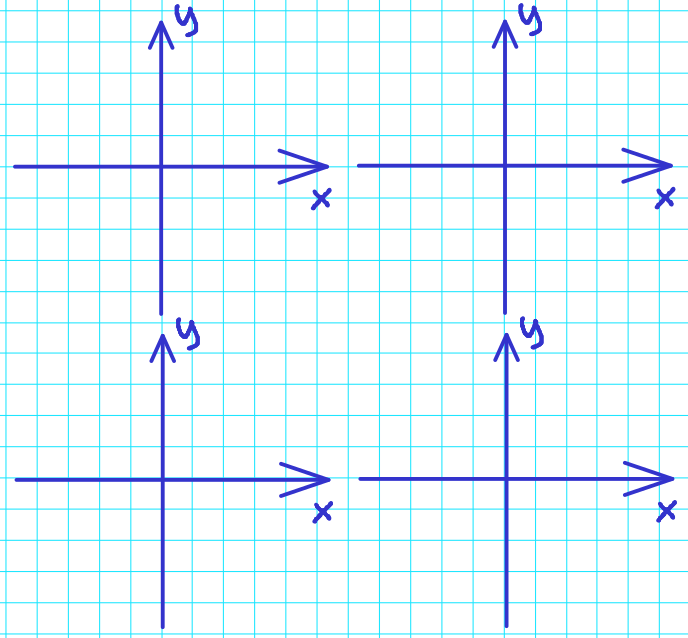
\includegraphics[width=8.5cm]{allg/funktionen/img/potenzfct/potenzFunktionenLeer.png}\hfill{}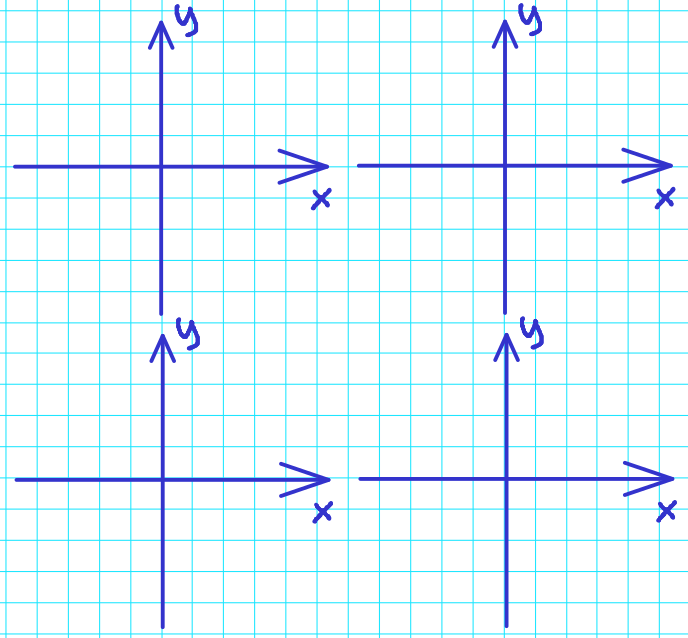
\includegraphics[width=8.5cm]{allg/funktionen/img/potenzfct/potenzFunktionenLeer.png}
}%% END Trainer


\subsection*{Aufgaben}
\AadBMTA{307}{25. b) c), 26. a)\TALS{ b)}, 27. b) c)\TALS{, 33*}}

\newpage


\newpage
\newpage
%%
%% 2019 07 04 Ph. G. Freimann
%%

\section{Exponentialfunktionen}\index{Funktion!Exponentialfunktion}\index{Exponentialfunktionen}
\sectuntertitel{Go viral!}
%%%%%%%%%%%%%%%%%%%%%%%%%%%%%%%%%%%%%%%%%%%%%%%%%%%%%%%%%%%%%%%%%%%%%%%%%%%%%%%%%
\subsection*{Lernziele}

\begin{itemize}
\item Definition Exponentialfunktion
\item Koeffizienten interpretieren
\item Graph: Symmetrien, Polstellen, Asymptoten, Schnittpunkte mit
  Achsen
  \item Basiswechsel
\end{itemize}

\TadBMTA{322}{19}
%%\TALS{(\cite{frommenwiler17alg} S.215 (Kap. 3.10))}
%%\GESO{(\cite{marthaler21alg}       S.322 (Kap. 19))}
\newpage

\subsection{Aussehen von Exponetialfunktionen}


Zeichnen Sie $f: y=2^x$ und $g: y=1.4^x$ ins selbe Koordinatensystem:


\bbwGraph{-5}{5}{-1}{5}{
\TRAINER{  \bbwFuncC{pow(2.0,\x)}{-3.5:2.1}{blue}
  \bbwFuncC{pow(1.4,\x)}{-3.5:3}{green}
  \bbwLetter{1,3}{$f$}{blue}
  \bbwLetter{2.5,2}{$g$}{green}
}%% end TRAINER
}%% end graph

\begin{definition}{Exponentialfunktion}{}\index{Exponentialfunktionen!Definition}
  Eine Funktion der Form $$f(x): x \mapsto a^x$$
  bzw. $$y = a^x$$
  mit $a\in \mathbb{R}^{+}\backslash\{1\}$ heißt \textbf{Exponentialfunktion}.
\end{definition}


\begin{bemerkung}{Zunahmefaktor}{}\index{Zunahmefaktor|textbf}
Der Parameter $a$ gibt den Wachstumsfaktor pro Zeiteinheit $e_x$ an.
\end{bemerkung}


\subsubsection*{Aufgaben}
\GESO{\olatLinkArbeitsblatt{Exponentialfunktionen}{https://olat.bms-w.ch/auth/RepositoryEntry/6029794/CourseNode/106029175831971}{Kap. 1.2:
    Einfache Wachstumsprozesse: Aufgaben 4. bis 6.}}
\TALS{\olatLinkArbeitsblatt{Exponentialfunktionen}{https://olat.bms-w.ch/auth/RepositoryEntry/6029786/CourseNode/106029175777725}{Kap. 1.2:
    Einfache Wachstumsprozesse: Aufgaben 4. bis 6.}}

\newpage

\subsection{Formen der Darstellung}
Zeichnen Sie die Funktionen $f: y=2^x$, $g: y=2^{-x}$ und $h: y=\left(\frac12\right)^x$ in dasselbe Koordinatensystem:

\bbwGraph{-6}{6}{-1}{5}{
  \TRAINER{\bbwFuncC{exp(0.69314718*\x)}{-6:2}{blue}}
  \TRAINER{\bbwFuncC{exp(-0.69314718*\x)}{-2:6}{red} }
  \TRAINER{\bbwLetter{1.5,4}{2^x}{blue}}
  \TRAINER{\bbwLetter{-5,4}{g(x)=2^{-x}=\left(\frac{1}{2}\right)^x=h(x)}{red}}
}

Bemerkung: \TRAINER{$$2^{-x} = \frac1{2^x} = \frac{1^x}{2^x}= \left(\frac12\right)^x$$}
\newpage



\subsubsection{Umkehrung (Optional)}
Um aus einem Wachstum einen Zerfall zu modellieren können wir entweder
die Zeitachse umdrehen oder den Kehrwert der Basis verwenden.
umgedreht werden:

Mit $d := \frac1a $ gilt:

\begin{center}
  \fbox{$a^{+t} = \left(\frac1a\right)^{-t} = d^{-t} $}
\end{center}

\newpage

\newpage

\subsection{Verschiebung und Streckung \GESO{(optional)}}

Eine Verschiebung der Exponentialfunktion $y=b\cdot{}a^x$ in der Zeit ($x$-Richtung) kann auch in Form einer Veränderung der Startfaktors $b$ umgeschrieben werden.

Verschieben wir \zB $$y=2^x$$ um fünf Einheiten nach rechts, so liest sich die neue Funktionsgleichung wie folgt:
$$y=2^{x-5}.$$

(Zeichnen Sie in \texttt{geogebra.org} a) $y=2^x$ und b) $y=2^{x-5}$.)

Dies kann jedoch auch umgeschrieben werden:

$$2^{x-5} = 2^x \cdot{} 2^{-5} = 2^{-5} \cdot{} 2^x = \frac{1}{2^5} \cdot{} 2^x =
\frac{1}{32}\cdot{}2^x$$

\bbwCenterGraphic{8cm}{allg/funktionen/img/exp/verschiebung_gleich_streckung.png}
Bildlegende: Eine Verschiebung ($x$-Richtung) der Exponentialfunktion entspricht einer Stauchung ($y$-Richtung) der selben Exponentialfunktion.

\TALS{Es gilt hier $$a^{x-b}=\frac{a^x}{k}$$ mit
$k=a^b$ und mit $b=\log_a(k)$.}

\newpage


\subsection{Punkte einsetzen\GESO{ (optional)}}
Wie bei den linearen Funktionen oder bei den Potenzfunktionen können auch Exponentialfunktionen gefunden werden, wenn bereits Punkte auf dem Graphen bekannt sind:

\textbf{Referenzaufgabe}

Finden Sie die Parameter $a$ und $b$ der Exponentialfunktion
$$f: y=b\cdot{}a^x$$
wenn Sie wissen, dass die Funktion durch die Punkte $P=(2|4)$ und $Q=(-1|2)$ verläuft:

\TNTeop{
  In Gleichung einsetzen:

  \gleichungZZ{4}{b\cdot{}a^2}{2}{b\cdot{}a^{-1}}

  Einsetzverfahren: Zum Beispiel aus der zweiten Gleichung das $b$ ermitteln...
  $$b = 2 a (III)$$
  ... und in die erste Gleichung einsetzen:

$$4 = 2a\cdot{} a^2$$
  $$2 = a^3$$
  $$a=\sqrt[3]{2}$$
  In (III) einsetzen:

  $$b = 2 \sqrt[3]{2}$$

  Ergo: $$f(x) = b\cdot{}a^x = 2\cdot{}\sqrt[3]{2} \cdot{} \left(\sqrt[3]2\right)^x \approx 2.5198 \cdot{} 1.2599^x$$
}

\subsection*{Aufgaben}
%%\AadBMTA{334}{10. a) b)\TALS{ e)}\GESO{ f)}}
\GESO{\olatLinkArbeitsblatt{Exponentialfunktionen}{https://olat.bms-w.ch/auth/RepositoryEntry/6029794/CourseNode/106029175831971}{Kap. 2.1: E-Funktion / Punkte-Aufgaben Aufg 26. a) b) ($e^{qt}$ optional) und Aufg. 27.}}
\TALS{\olatLinkArbeitsblatt{Exponentialfunktionen}{https://olat.bms-w.ch/auth/RepositoryEntry/6029786/CourseNode/106029175777725}{Kap. 2.1: E-Funktion / Punkte-Aufgaben Aufg 26. a) b) ($e^{qt}$ optional) und Aufg. 27.}}

\AadBMTA{336}{23. d}

\newpage

\newpage
%% 2019 07 04 Ph. G. Freimann
%%

\section{Wachstum und Zerfall}\index{Wachstum}\index{Zerfall}
\sectuntertitel{Sagt ein großer Stift zum kleinen Stift: ``Wachsmalstift!''}

%%%%%%%%%%%%%%%%%%%%%%%%%%%%%%%%%%%%%%%%%%%%%%%%%%%%%%%%%%%%%%%%%%%%%%%%%%%%%%%%%

\TRAINER{
  Video \href{https://www.youtube.com/watch?v=TMaLuks8dxw}{MatheMann}
Wo schneiden sich $x^3$ und $e^x$?}%%
\subsection*{Lernziele}

\begin{itemize}
\item Zinseszins
\item Wachstums-, Zerfallsprozesse
\item Verdoppelungs- und Halbwertszeiten
%%\item Basiswechsel
\end{itemize}

\TadBMTA{342}{20}
%%\TALS{(\cite{frommenwiler17alg} S.221 (Kap. Exponentielles Wachstum))}
%%\TALS{(\cite{frommenwiler17alg} S.223 (Kap. Exponentielle Abnahme))}
%%\TALS{(\cite{frommenwiler17alg} S.225 (Kap. Zinseszins))}
%%\GESO{(\cite{marthaler21alg}       S.342 (Kap. 20))}

\newpage


\subsection{Beispiele}
Bei Wachstumsprozessen sprechen wir dann von einer exponentiellen
Zunahme, wenn die Zunahme pro Zeiteinheit immer proportional zum aktuellen Bestand ist.

\begin{itemize}
\item \Lueckentext{Zinseszins}
\item \Lueckentext{Frequenzen in der temperierten Stimmung
  (Musik). Zunahme der Frequenz pro Halbtonschritt.}
\item \Lueckentext{Keime in der Kuhmilch; Ansteckungsbedingte Krankheitsfälle (\zB viral)}
\item \Lueckentext{Algenbefall in Teichen}
\item \Lueckentext{Generell Populationen: Flechten, Pilze}
\item \Lueckentext{(ungebremstes) Bevölkerungswachstum / bzw. Tierpopulation}
\item \Lueckentext{\dotfill}
\end{itemize}


\GESO{\olatLinkArbeitsblatt{Exponentialfunktionen}{https://olat.bms-w.ch/auth/RepositoryEntry/6029794/CourseNode/106029175831971}{Kap. 1.1:
    Voraussetzungen: Aufgaben 1. bis 3.}}
\TALS{\olatLinkArbeitsblatt{Exponentialfunktionen}{https://olat.bms-w.ch/auth/RepositoryEntry/6029786/CourseNode/106029175777725}{Kap. 1.1:
    Voraussetzungen: Aufgaben 1. bis 3.}}


\newpage

\subsection{Einstiegsbeispiel Taschengeld}

Bei Familie Cash kann man aussuchen, wie sich sein Taschengeld über
die Jahre «vermehrt». Mani wählt Variante A. Bei Varante A erhält man
CHF 1.- im ersten Jahr, CHF 2.- im 2. Jahr, CHF 3.- im 3. Jahr und so
weiter bis zur abgeschlossenen Grundbildung im 13. Jahr CHF 13.-.

Carla wählt Variante B. Bei der Variante B erhält Carla auch CHF 1.-
im ersten Jahr, dann aber jedes Jahr 30\% mehr, als im Vorjahr.

a) Wird Carla vor Ende der Grundbildung jemals mehr als Mani erhalten?

\LoesungsRaumLang{Ja, im 10. Schuljahr}

b) Wer hat über alle Jahre mehr Taschengeld?

\LoesungsRaumLang{Carla wird mehr haben}

c) Skizzieren Sie beide Varianten:

\TRAINER{\bbwCenterGraphic{13cm}{allg/funktionen/img/taschengeldAusgefuellt.png}}
\noTRAINER{\bbwCenterGraphic{16cm}{allg/funktionen/img/taschengeld.png}}

\TRAINER{Optional: Zeige mit Geogebra (\texttt{geogebra.org}) $x^2$ vs. $1.2^x$. Fazit:
  Exponentielles Wachstum überholt jegliche Potenzfunktion.}



\newpage

Zeichnen Sie $f: y=2^x$ und $g: y=1.4^x$ ins selbe Koordinatensystem:


\bbwGraph{-5}{5}{-1}{5}{
\TRAINER{  \bbwFuncC{pow(2.0,\x)}{-3.5:2.1}{blue}
  \bbwFuncC{pow(1.4,\x)}{-3.5:3}{green}
  \bbwLetter{1,3}{$f$}{blue}
  \bbwLetter{2.5,2}{$g$}{green}
}%% end TRAINER
}%% end graph

\begin{definition}{Exponentialfunktion}{}\index{Exponentialfunktionen!Definition}
  Eine Funktion der Form $$f(x): x \mapsto a^x$$
  bzw. $$y = a^x$$
  mit $a\in \mathbb{R}^{+}\backslash\{1\}$ heißt \textbf{Exponentialfunktion}.
\end{definition}


\begin{bemerkung}{Wachstumsfaktor}{}\index{Wachstumsfaktor}
Der Parameter $a$ gibt den Wachstumsfaktor pro Zeiteinheit $e_x$ an.
\end{bemerkung}


\subsubsection*{Aufgaben}
\GESO{\olatLinkArbeitsblatt{Exponentialfunktionen}{https://olat.bms-w.ch/auth/RepositoryEntry/6029794/CourseNode/106029175831971}{Kap. 1.2:
    Einfache Wachstumsprozesse: Aufgaben 4. bis 6.}}
\TALS{\olatLinkArbeitsblatt{Exponentialfunktionen}{https://olat.bms-w.ch/auth/RepositoryEntry/6029786/CourseNode/106029175777725}{Kap. 1.2:
    Einfache Wachstumsprozesse: Aufgaben 4. bis 6.}}


\newpage

\subsection{Exponentieller Zerfall}\label{zerfallsfunktion}
Die Funktion $f(x): x \mapsto y = d^{-x}$ ist eine
Exponentialfunktion, die gegen Null geht.

\bbwFunction{-4}{4}{-1}{8}{exp(-\x)}{-2:4}

\begin{bemerkung}{}{}
Oft wird bei Wachstumsprozessen die Zeitachse auch mit $t$ statt $x$ bezeichnet: $t$ steht für \textit{time}.
\end{bemerkung}

\newpage

\subsubsection{Beispiele}
\begin{itemize}
	\item \Lueckentext{Zinsliche Abschreibungen (\zB Wert eines Autos)}
	\item \Lueckentext{Radioaktiver Zerfall}
	\item \Lueckentext{Lichtintensität in Medium (Gas / Flüssigkeit / Glasfaser), dies gilt vertikal, wie auch horizontal}
	\item \Lueckentext{Atmosphärischer Luftdruck in Metern über Meer}
  \item \Lueckentext{Entladen einer Batterie bzw. eines Kondensators}
  \item \Lueckentext{Sauerstoffkonzentration in Seen (\zB Herbst bei kontinuierlicher Abnahme)}
  \item \Lueckentext{Abnahme des Bierschaums im Glas}
  \item \Lueckentext{Mischen, wie im Sirup-Beispiel\totalref{sirup_beispiel}}
  \item \Lueckentext{«Halbwertszeit des Wissens» ;-)}
  \item \Lueckentext{\dotfill}
\end{itemize}

\newpage



Zeichnen Sie die Funktionen $f: y=2^x$, $g: y=2^{-x}$ und $h: y=\left(\frac12\right)^x$ in dasselbe Koordinatensystem:

\bbwGraph{-6}{6}{-1}{5}{
  \TRAINER{\bbwFuncC{exp(0.69314718*\x)}{-6:2}{blue}}
  \TRAINER{\bbwFuncC{exp(-0.69314718*\x)}{-2:6}{red} }
  \TRAINER{\bbwLetter{1.5,4}{2^x}{blue}}
  \TRAINER{\bbwLetter{-5,4}{g(x)=2^{-x}=\left(\frac{1}{2}\right)^x=h(x)}{red}}
}

Bemerkung: \TRAINER{$$2^{-x} = \frac1{2^x} = \frac{1^x}{2^x}= \left(\frac12\right)^x$$}
\newpage

\subsubsection{Grundform} \index{Exponentieller Prozess! Grundform}
Die Grundform für Zerfallsprozesse lautet:

\begin{definition}{Zerfall}{}\index{Zerfall}
  Die Grundform des exponentiellen Zerfalls wird beschrieben durch die Funktion
$$f(x): x \mapsto a^x$$
  bzw.
  $$y = a^x$$
\end{definition}


\begin{gesetz}{Wachstum vs. Zerfall}{}

  Der einzige Unterschied bei Wachstums- bzw Zerfallsprozessen ist der
  Faktor $a$:

  \begin{itemize}
    \item \LoesungsRaumLen{40mm}{$a>1$: Wachstum}\vspace{3mm}
    \item \LoesungsRaumLen{40mm}{$0<a<1$: Zerfall}
  \end{itemize}
  
\end{gesetz}

\begin{bemerkung}{$x$-Richtung}{}
  Exponentielle Prozesse laufen meist in der Zeit ab. Somit wird
  die $x$-Achse zur Zeitachse und meist mit $t$ (Time) bezeichnet:
  $$f(t) = a^t$$
  \end{bemerkung}


\subsubsection{Umkehrung (Optional)}
Um aus einem Wachstum einen Zerfall zu modellieren können wir entweder
die Zeitachse umdrehen oder den Kehrwert der Basis verwenden.
umgedreht werden:

Mit $d := \frac1a $ gilt:

\begin{center}
  \fbox{$a^{+t} = \left(\frac1a\right)^{-t} = d^{-t} $}
\end{center}

\newpage

\subsection*{Aufgaben}
%%\TALSAadBMTA{223ff}{840., 841., 843., 844. und 846.}

\GESO{\olatLinkArbeitsblatt{Exponentialfunktionen}{https://olat.bms-w.ch/auth/RepositoryEntry/6029794/CourseNode/106029175831971}{Kap. 1.3: Zerfall: Aufg. 7., 8. und 9.}}
\TALS{\olatLinkArbeitsblatt{Exponentialfunktionen}{https://olat.bms-w.ch/auth/RepositoryEntry/6029786/CourseNode/106029175777725}{Kap. 1.3: Zerfall: Aufg. 7. 8. und 9.}}

\AadBMTA{354}{9. (Bauchspeicheldrüse)}
\olatLinkGESOKompendium{3.4.1}{27ff}{33., 35., 36., 39. und 41.}

\newpage
%% Sirup-Beispiel
\subsection{Mischtank}\index{Mischtank}\index{Sirup}\label{sirup_beispiel}
Wird ein Glas Wasser in ein Glas Sirup geschüttet, so

\TRAINER{\bbwCenterGraphic{5cm}{allg/alg/potenzen_wurzeln/img/Schwapp.png}}%%
\noTRAINER{\bbwCenterGraphic{5cm}{allg/alg/potenzen_wurzeln/img/SchwappOhneFormel.png}}

geschieht erst mal etwas eher klebriges:
\begin{itemize}
  \item Das Wasser verdrängt den Sirup und
  \item das Sirupglas schwappt über.
\end{itemize}

Wenn man nun gleichzeitig im Sirupglas
umrührt, so mischt sich das Wasser mit dem Sirup und je länger man
Wasser einschüttet, umso verdünnter wird der Sirup.


Wie viel Sirup bleibt im Glas?

\TNT{2.4}{
Am Ende bleibt ein
Verhältnis von Wasser : Sirup = $\left(1-\frac{1}{e}\right) : \left(\frac{1}{e}\right)$
\vspace{1.5cm}
}

Diese Konstante wird oft in großen chemischen Mischtanks verwendet,
gibt aber auch ein Maß an, wenn \zB in einer Minergie-Wohnung die Luft
ausgetauscht wird. Wenn nämlich das Volumen der Wohnung einmal neu hineingepumpt (bzw. weggeblasen) wurde während sich alte die Luft im Haus permanent mit der neuen vermischt, so ist noch ein Anteil von \TRAINER{$\frac{1}{e}$}\noTRAINER{ ..... } der alten Luft im Haus.
\newpage


\textbf{Begründung:}\\
1. Gedanke: Jedes eingefüllte Glas, vermindert die vorhandene
Sirupkonzentration um den selben Faktor. Ergo handelt es sich um
einen exponentiellen Zerfall.

\leserluft

2. Gedanke: Wir tauschen drei Mal $\frac13$ aus. Nehmen also im
\begin{itemize}
\item \textbf{ersten Schritt} $\frac13$ des Sirups weg (und ersetzen diesen mit Wasser).
  Es bleiben $\frac23$ Sirup. Den Rest füllen wir mit Wasser auf.
\item Im \textbf{zweiten Schritt} nehmen wir $\frac13$ des Gemisches
weg; es verbleiben also $\frac23$ von $\frac23$ an
Sirup-Konzentrat. Der Rest wird immer wieder mit Wasser aufgefüllt. Mit
anderen Worten: Es bleiben $\frac23 \cdot \frac23
= \left(\frac23\right)^2$ an Sirup\footnote{Man könnte hier auch argumentieren mit: «Wir nehmen von den $\frac23$ einen Drittel weg»: $\frac23 - (\frac13$ von $\frac23)$ = $\frac23 - (\frac13 \cdot\frac23) = \frac23 \cdot(1-\frac13)=\frac23\cdot\frac23$}.
\item Im \textbf{dritten Schritt} entnehmen wir wieder $\frac13$ des
Gemisches; es verbleiben wieder $\frac23$ vom bisherigen Sirup, also
$\frac23$ von $(\frac23)^2$ also $\left(\frac23\right)^3$.

Beim dreistufigen Gedankenexperiment verbleiben
$\left(\frac23\right)^3 = \left(1-\frac13\right)^3$ der ursprünglichen Konzentration.
\end{itemize}
\leserluft

3. Gedanke: Das Experiment vom vorherigen Gedanken können wir natürlich auch mit immer kleineren\TALS{, sogenannten infinitesimalen,} Schritten durchführen.
Mit Centilitern \zB im dl-Glas ersetzen wir 10 Mal je $\frac1{10}$. 
So verbleibt am Schluss $\left(1-\frac{1}{10}\right)^{10}\approx 0.35$ Sirup.

\GESO{Wenn wir (\zB mit dem Taschenrechner) die Schrittanzahl immer weiter vergrößern (und somit die pro Schritt ausgetauschte Menge immer verkleinern), so ergibt sich für 1000 Schritte ein Verhältnis von $\left(1-\frac{1}{1000}\right)^{1000}\approx 0.3677 \approx \frac1{\e}$. }
\TALS{Wenn wir die Schritte permanent erhöhen (und gegen Unendlich gehen lassen), so erhalten wir den Grenzwert (lat. Limes) von

$$\lim_{n\rightarrow\infty} \left(1-\frac{1}{n}\right)^n = \frac1{\e}$$
}
\newpage

\textbf{Aufgabe 1: Sirup}\\
Wie viel Wasser muss eingeschüttet werden, damit das auf der Flasche
angegebene Verhältnis von 1:6 (1 Teil Sirup, 6 Teile Wasser) zustande
kommt?

\TNT{8}{
Bei 1x Schütten, erhalten wir $\left(\frac{1}{\e}\right)^1$ Anteil Sirup.

Bei 2x Schütten, erhalten wir $\left(\frac{1}{\e}\right)^2$ Anteil Sirup.

Somit erhalten wir den Siebtel (1:6 = $\frac17$-Anteil) indem wir die
folgende Exponentialgleichung lösen:

$$\frac17 = \left(\frac{1}{\e}\right)^n$$
Diese Gleichung lösen wir, indem wir beidseitig logarithmieren und so
erhalten wir den einzuschüttenden Teil $$n=\ln(7)\approx{1.946}.$$
}%% END TNT

\textbf{Aufgabe 2: Minerige-Haus}\\
Wenn wir also wissen wollen, wie viel Luft in ein Minergiehaus
eingepumpt werden muss, damit nur noch 1 Promille der alten Luft
vorhanden ist, so erhalten wir
\TNTeop{
  $$\text{Volumen Neuluft} = \text{Wohnungsvolumen}\cdot{}\ln(1000)$$
  $$\ln(10000) \approx 6.9$$
} %% end TNT


\newpage

\newpage


\subsection{Startwert}\index{Startwerte!bei Wachstums- und Zerfallsprozessen}

Die bisher betrachteten Exponentialfunktionen haben für den Wert $x=0$ (bzw. $t=0$) immer den
$y$-Wert = 1 bzw. 100\%.
Da in der Praxis meist konkrete Werte vorgegeben sind verwenden wir
eine \textbf{allgemeinere Form der Exponentialfunktion}.

\subsubsection{Einstiegsbeispiel}

\begin{beispiel}{Pilz}{}
  Ein Pilzbefall an einer Wand nehme täglich um 23\% der Fläche
  zu\footnote{Je nach Organismus ist auch ein quadratisches Wachstum
  vorhanden, doch für unser Experiment verwenden wir exponentielles Wachstum.}.
  Anfänglich wird eine Fläche von $35$ $\text{cm}^2$ gemessen.
  Welche Fläche ist nach einem, nach zwei, nach fünf, nach zehn
  bzw. nach $n$ 
  Tagen zu erwarten?

  \TNT{6}{Ein  Tag:   $35\cdot{} 1.23^1    =          43.05 \text{cm}^2$\\
          Zwei Tage:  $35\cdot{} 1.23^2   \approx{}  52.95 \text{cm}^2$\\
          Fünf Tage:  $35\cdot{} 1.23^5   \approx{}  98.54 \text{cm}^2$\\
          Zehn Tage:  $35\cdot{} 1.23^{10} \approx{} 277.4 \text{cm}^2$\\
          $n$  Tage:  $35\cdot{} 1.23^n = 35\cdot{}1.23^n$}%% END TNT

  Wann wird die ganze Wand ($6 \text{ m}^2$) mit dem Pilz befallen
  sein?
  
\TNT{6}{$6 \text{ m}^2 = 60\,000 \text{ cm}^2$
     
     ergo: $60\,000 = 35 \cdot{} 1.23^n$

     (durch 35 teilen, dann logarithmieren)

     $$\frac{60\,000}{35} = 1.23^n$$

     $$n = \log_{1.23}\left(\frac{60\,000}{35}\right) \approx 35.97 \text{Tage}$$

   }%% END TNT

\end{beispiel}

\newpage


\begin{gesetz}{Exponentialfunktion mit frei wählbarem Startwert}{}
$$f: y = \LoesungsRaumLen{40mm}{b\cdot{}a^x}$$

Auch hier gibt der Parameter $a$ den Wachstumsfaktor pro Zeiteinheit $e_x$ an.

Dabei ist $b$ der Startwert zum Zeitpunkt $x$ = 0.
\end{gesetz}


\noTRAINER{\bbwCenterGraphic{8cm}{allg/funktionen/img/exp/b_faktor.png}}
\TRAINER{\bbwCenterGraphic{8cm}{allg/funktionen/img/exp/b_faktor_trainer.png}}

\begin{bemerkung}{Wachstumsfaktor}{}{}
Werden zwei $x$ Positionen mit Differenz 1 (=$e_x$) betrachtet, so sind
die zugehörige $y$-Werte um \textbf{Faktor} $a$ auseinander.
\end{bemerkung}

Begründung:
\TNTeop{
  Gegeben $x_1$ und $x_2 = x_1 + 1$. So ist

  $y_1 = b\cdot{}a^{x_1}$ und $y_2 = b\cdot{}a^{x_2}$.

  Setzen wir nun $x_1 + 1$ für $x_2$ ein, so erhalten wir:

  $$y_2 = f(x_2) = b\cdot{}a^{x_2} = b\cdot{} a^{x_1+1} =  b\cdot{}a^{x_1} \cdot{} a^1 = y_1\cdotp{} a$$
}
\newpage


\subsection*{Aufgaben}

\GESO{\olatLinkArbeitsblatt{Exponentialfunktionen}{https://olat.bms-w.ch/auth/RepositoryEntry/6029794/CourseNode/106029175831971}{Kap. 1.4:
    Frei wählbarer Startwert: Aufg. 10. Gummiball; 11. Neophytenplage;
    12: Tierpopulation; 13. Licht im Wasser;  weitere Aufgaben 14. bis 17.}}
\TALS{\olatLinkArbeitsblatt{Exponentialfunktionen}{https://olat.bms-w.ch/auth/RepositoryEntry/6029786/CourseNode/106029175777725}{Kap. 1.4:
    Frei wählbarer Startwert: Aufg. 10. Gummiball; 13. Licht im Wasser. 14. Federpendel; 15. Luftdruck; weitere Aufgaben aus
    Kap. 1.4.}}
 
  \AadBMTA{338}{29. (Bierschaum)}
  \AadBMTA{353}{6. (C-14 Methode)}

  Als Vorbereitung zur allgemeinen Wachstumsfunktion:
  \AadBMTA{207}{10. (Algen)}

\newpage


\subsection{Beobachtungszeitspanne}
\subsubsection{Einstgiesbeispiel}
\bbwCenterGraphic{17cm}{allg/funktionen/img/tuerlersee2.jpg}
\begin{center}{\small Legende: Türlersee April 2022}\end{center}

Der Türlersee ist ein kleiner See im Reppischtal. Seine Oberfläche
begann sich vor einigen Jahrzehnten stark mit Algen\footnote{Genau
  genommen handelte es sich um Zooplanktonbiomasse zwischen 1982 und 1994, doch als
  Idee zur Exponentialfunktion sollte ein ungefähres Flächenmodell reichen.} zu bedecken.

Anfänglich (zum Zeitpunkt $t=0$) waren gerade mal 20$m^2$ bedeckt. Doch nach fünf Tagen hatte sich diese Fläche verdoppelt und nach weiteren fünf Tagen nochmals verdoppelt (also insgesamt vervierfacht).

Füllen Sie die (prognostizierte) Wertetabelle für 30 Tage ein:

\def\spaceX{\,\,\,\,\,\,\,\,\,\,}
\newcommand\tuerlerB[1]{\noTRAINER{\spaceX}\TRAINER{#1}}
\begin{tabular}{l|c|c|c|c|c|c|c}
  $t$:  & 0 & 5 & 10 & 15 & 20 & 25 & 30 \\
  \hline
  $m^2$ & \tuerlerB{20}  & \tuerlerB{40}  &   \tuerlerB{80}  &  \tuerlerB{160}  &  \tuerlerB{320}  &  \tuerlerB{640}  &  \tuerlerB{1280} \\
\end{tabular}

\newpage
Zeichnen Sie die Algenpopulation als Graph in eine Koordinatensystem
(beginnen Sie mit dem Ursprung ganz links unten. $x$-Achse in Tagen ($t$). $y$-Achse in $\text{m}^2$.

\noTRAINER{\bbwCenterGraphic{170mm}{allg/funktionen/img/exp/WachstumTuerlerseeLeer.png}}
\TRAINER{\bbwCenterGraphic{10cm}{allg/funktionen/img/exp/tuerlerAlgen.png}}
\newpage

\textbf{Funktionsgleichung}

Wir betrachten die selbe Algenpopulation mit einer
Ver\textbf{\color{blue}dopplung} der Fläche alle \textbf{\color{red}fünf} Tage bei einer
Startfläche von \textbf{\color{green}zwanzig} $\text{m}^2$.

Geben Sie eine Funktionsgleichung an, welche das Wachstum der
Algenpopulation beschreibt...



\begin{bbwFillInTabular}{c|c|c||c|c|c|c|c|c|c|c}\hline
  Tage      & $t$ & \cellcolor{gray!75}\noTRAINER{\hspace{2cm}} & 0            & \tiny{1-4} & 5            & \tiny{6-9} & 10           & \tiny{11-14} & 15           &\\\hline
  Fläche     & $A$ & \TRAINER{$20\cdot v$}    &
  \TRAINER{20}\noTRAINER{\hspace{15mm}} &  \cellcolor{gray!75}    &
  \TRAINER{40}\noTRAINER{\hspace{15mm}} &    \cellcolor{gray!75}  &
  \TRAINER{80}\noTRAINER{\hspace{15mm}} &         \cellcolor{gray!75}       &
  \TRAINER{160}\noTRAINER{\hspace{15mm}} &\\\hline
  Faktor    & $v$ & \TRAINER{$v=2^z$}    & \TRAINER{1}  &  \cellcolor{gray!75}    & \TRAINER{2}  &   \cellcolor{gray!75}   & \TRAINER{4}  &    \cellcolor{gray!75}            & \TRAINER{8} &\\\hline
  Intervalle & $z$ & \TRAINER{$z=\frac{t}{5}$}    & \TRAINER{0}  &  \cellcolor{gray!75}    & \TRAINER{1.}  & \cellcolor{gray!75}     & \TRAINER{2.}  &   \cellcolor{gray!75}             & \TRAINER{3.} &\\\hline
  Potenz     &\TRAINER{$2^z$} & \TRAINER{$2^\frac{t}{5}$}     & \TRAINER{$2^0$}  &   \cellcolor{gray!75}   & \TRAINER{$2^1$}  &   \cellcolor{gray!75}   & \TRAINER{$2^2$}  &  \cellcolor{gray!75}              & \TRAINER{$2^3$} &\\\hline
\end{bbwFillInTabular}

\TRAINER{Falls nicht mit Tabelle: 1. Tipp $f(0)=20; f(5)=40;
  f(10)=80;...$, dann 2. Tipp $f_B(0) = 20; f_B(1)=40; ...$ $B$=Anzahl
  Beobachtungsintervalle}

\leserluft
\begin{center}
  $f(t):\,\,\, y=\LoesungsRaumLang{{\color{green}20}\cdot{} {\color{blue}2} ^{\frac{t}{\color{red}5}}}$
  \end{center}
\TNT{4}{
Dabei bezeichnet\\20 den Startwert,\\2 den Zunahmefaktor und \\5 die Beobachtungszeitspanne.}%%

Merke:
\TNTeop{Ich muss für $t$ fünf Tage einsetzen, um auf eine Verdopplung
  zu kommen.

  Setze ich $t=0$ ein, so erhalte ich den Startwert zwanzig m$^2$.
}
%%%%%%%%%%%%%%%%%%%%%%%%%%%%%%%%%%%%%%%%%%%%%%%%%%%%%%%%%%%%%%%%%%%%%%%%%%%%%%%%%%%%%%%%%%%%%%%%%%%%

\subsubsection{Exponentieller Prozess (allgemein)}\index{Exponentieller Prozess! allgemeine Form}

\begin{gesetz}{Wachstumsprozess}{}
  Die Funktion

  $$y = f(t) = \LoesungsRaumLen{40mm}{b\cdot{}a^{\frac{t}{\tau}}}$$
  
  beschreibt einen allgemeinen exponentiellen Wachstumsprozess mit
  $$   a=\LoesungsRaumLen{50mm}{\text{Wachstumsfaktor während } \tau \text{ Tagen} }$$
  $$   b=\LoesungsRaumLen{50mm}{\text{Startwert}}$$
  $$\tau=\LoesungsRaumLen{50mm}{\text{Beobachtungszeitspanne}}$$
\end{gesetz}

Alternativ «die harte Tour» (ohne das $\tau$ mit anderer Basis):

\TNTeop{


  $$f(t) = b\cdot{}A^t$$

  $A$ = Faktor pro Tag, $t$ = Anzahl Tage, Startwert $b=f(0)$
  
  Bsp.: Die Algenzahl verdoppelt sich alle fünf Tage:

  $$f(5)        = 2 \cdot{} f(0)$$
  $$b\cdot{}A^5 = 2 \cdot{} b $$

  $$A^5 = 2$$

  $$A = \sqrt[5]{2} = 2^{\frac15} \approx 1.1487$$

  Einsetzen in $f(t) = b\cdot{} A^t$

  $$f(t) = b\cdot{} \left(\sqrt[5]{2}\right)^t  = b\cdot{}
  \left(2^{\frac15}\right)^t=b\cdot{} 2^{\frac{t}5} \approx b\cdot{} 1.1487^t$$

}%% end TNTeop


\newpage

\subsubsection{Graphische Erläuterung (optional)}


\begin{tabular}{cc}%%
  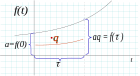
\includegraphics[width=9cm]{allg/funktionen/img/exp/exponentielles_wachstum.png} &
  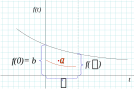
\includegraphics[width=7cm]{allg/funktionen/img/exp/exponentieller_zerfall.png}\\
\end{tabular}

%%\bbwCenterGraphic{10cm}{allg/funktionen/img/exp/exponentieller_zerfall.png}
%%\bbwCenterGraphic{11cm}{allg/funktionen/img/exp/exponentielles_wachstum.png}

Dabei sind
\begin{itemize}
\item $b=f(0)$ der Anfangsbestand zum Zeitpunkt $t$ = 0.
\item $\tau$ ist die typische Zeitspanne zwischen zwei Beobachtungszeitpunkten (zum Beispiel zwischen Wert und dessen Verdopplung). Beispiele:
  \begin{itemize}
  \item Verdoppeln in 3 Stunden: $a=2$ und $\tau = 3\, \text{h}$
    ($\text{h}$ = Stunden)
  \item Verfünf"|fachen einer Viertelstunde (= 15 Minuten): $a=5$ und
    $\tau=\frac{1}{4}\, \text{h}$
  \end{itemize}
  Meist ist die Beobachtungszeit gleichzeitig die Maßeinheit (\zB
  Veränderung pro Stunde). Dann ist unser $\tau=1$ und die Formel
  vereinfacht sich zu $f(t) = b\cdot{}a^t$.
\item $a$ ist der Zunahmefaktor zwischen zwei Beobachtungszeitpunkten (Beispiel $a=2$ bei Verdoppelungsprozessen).
  $a$ berechnet sich durch den Quotienten zwischen zwei
  Beobachtungswerten $a = \frac{f(\tau)}{f(0)} =\frac{m}{b}$.
\item
  Dabei ist $m$ der Messwert zum Zeitpunkt $\tau$.
\item $f(t)=b\cdot{}a^{\frac{t}{\tau}}$ ist der Wert (Anzahl, Fläche,
  Bestand, ...) zum Zeitpunkt
  $t$. 
\end{itemize}

Bemerkung: 
\TNTeop{
$\frac{m}b = \frac{f(\tau)}{f(0)}=\frac{b\cdot{}a^{\frac{\tau}{\tau}}}{b\cdot{}a^{\frac0{\tau}}}
  = \frac{a^1}{a^0} = \frac{a}{1} 
  = a$}%% END TNT
\newpage

\subsection{Referenzaufgabe}\index{Irland!Bevölkerungswachstum}
Irland hatte 1990 3.51 Mio. Einwohner. Im Jahr 2019 waren es bereits 4.93 Mio.

\textbf{Frage 1}: Was prognostizieren Sie für das Jahr 2025, wenn Sie von einem exponentiellen Wachstum ausgehen?

\noTRAINER{\bbwCenterGraphic{12cm}{allg/funktionen/img/exp/IrlandLeer.png}}%%

\TNTeop{
  Skizze:
  \bbwCenterGraphic{12cm}{allg/funktionen/img/exp/IrlandVoll.png}

  $\tau$ = 29 Jahre, Einheit = Jahre ($t$ in Jahren gemessen).
  
  $b=f(0) = 3.51$ [Mio EW] = Startwert (Taschenrechner STO).

  $m=f(\tau) = 4.93$ [Mio EW] = Messwert nach $\tau$ Jahren.

  $a=\frac{m}{b}=\frac{4.93}{3.51} \approx 1.4046$ pro 29 Jahre (Taschenrechner! STO). 

  $$f(t) = b\cdot{}a^\frac{t}{\tau}=b\cdot{}a^\frac{t}{29}$$


  TR Probe $b\cdot{}a^\frac{0}{29} = ? = 3.51$ 

  TR Probe $b\cdot{}a^\frac{29}{29} = ? = 4.93$ 

  Jahr 2025: $t=35$:

    $$f(35) = b\cdot{}a^\frac{35}{29}\approx 5.28899$$

}%% END TNT
\newpage

\subsection*{Aufgaben}

\GESO{\olatLinkArbeitsblatt{Exponentialfunktionen}{https://olat.bms-w.ch/auth/RepositoryEntry/6029794/CourseNode/106029175831971}{Kap. 1.5: Aufg. 18. a) b)}}
\TALS{\olatLinkArbeitsblatt{Exponentialfunktionen}{https://olat.bms-w.ch/auth/RepositoryEntry/6029786/CourseNode/106029175777725}{Kap. 1.5:     Aufg. 18. a) b) }}

\newpage

\textbf{Frage 2}: In wie vielen Jahren hat sich die Bevölkerung verdreifacht?

\TNTeop{
  Gesucht $T_3$ = Verdreifachungszeitpunkt.

  $$f(T_3) = 3\cdot{}f(0)$$

  Funktionsgleichung einsetzen:

  $$b\cdot{}a^\frac{T_3}{\tau} = 3\cdot{} b\cdot{} a^\frac0\tau$$

  Weil $a^{\frac{0}{\tau}} = 1$ folgt:

  $$b\cdot{}a^\frac{T_3}{\tau} = 3\cdot{} b$$

  $$a^\frac{T_3}{\tau} = 3$$

  Def. Logarithmus:

  $$\frac{T_3}{\tau} = \log_a(3)$$

$$T_3 = \tau\cdot{}\log_a(3) = 29\cdot{}\log_a(3) \approx 93.8$$
Die Bevölkerung wird sich voraussichtlich alle 94 Jahren
verdreifachen.

}%% END Trainer
\newpage

\subsection*{Aufgaben}
%%\TALSAadBMTA{221ff}{831 - 839}


\GESO{\olatLinkArbeitsblatt{Exponentialfunktionen}{https://olat.bms-w.ch/auth/RepositoryEntry/6029794/CourseNode/106029175831971}{Kap. 1.5:
    Aufg. 18. c), 19. - 21.}}
\TALS{\olatLinkArbeitsblatt{Exponentialfunktionen}{https://olat.bms-w.ch/auth/RepositoryEntry/6029786/CourseNode/106029175777725}{Kap. 1.5:
    Aufg. 18. c), 19. - 21. }}

\AadBMTA{338}{28. Bakterien}
\AadBMTA{352ff}{2. (Hasenpopulation), 7., 1. (optional)}
\olatLinkGESOKompendium{3.4}{27ff}{32., 34., 38., 40., 44., 45. und 46.}
\GESO{\aufgabenFarbe{Nullserie 2: Aufgabe 8.}}
\GESO{\aufgabenFarbe{Maturaprüfung 2017, Aufg. 12 (Raupen)\\
Maturaprüfung 2018 (Serie 3), Aufg. 11 (Müll)
}}



%% TODO Arbeitsblatt verlinken
%%\GESO{\olatLinkArbeitsblatt{Exponentialfunktionen}{https://olat.bms-w.ch/auth/RepositoryEntry/6029794/CourseNode/106029175831971}{Kap. 1.1: Voraussetzungen}}
%%\TALS{\olatLinkArbeitsblatt{Exponentialfunktionen}{https://olat.bms-w.ch/auth/RepositoryEntry/6029786/CourseNode/106029175777725}{Kap. 1.1: Voraussetzungen}}



\newpage

\subsection{Rate vs. Faktor
  II}\index{Rate}\index{Fatkor}\index{Zunahmefaktor}\index{Zunahmerate}
\totalref{RateZins1}

Den Unterschied von Zinsfuß (= Rate) und Zinsfaktor kennen wir bereits aus der Zinsrechnung.

So entspricht eine Zunahme von 12\% einem\\
Aufzinsungsfaktor von \LoesungsRaumLang{1.12}.

Wenn jedoch eine Beobachtung einer Zunahme von, sagen wir, 70\% innerhalb einer Viertelstunde beobachtet wird, so können wir uns fragen, um wie viel die Zunahme (als Rate oder Faktor) pro Zeiteinheit (hier Stunden) ist.


Füllen Sie dazu folgende Tabelle aus. Dabei bedeuten

\begin{tabular}{lp{14cm}}\hline
  Einheit & Stunden, Minuten, Meter, ... \\\hline
  $\tau$  & In dieser Zeitspanne (Stunden, Meter, ...) wird beobachtet \\\hline
  $p$     & Zunahme\textbf{rate}\index{Zunahmerate}\index{Rate} während $\tau$ Einheiten in \%. Ist $p$ negativ, handelt es sich um eine Abnahme\\\hline
  $a_\tau$ & Zunahme\textbf{faktor}\index{Zunahmefaktor} während $\tau$ Einheiten. Ist $a<1$, handelt es sich um einen Abnahmefaktor\\\hline
  $a_E$ (Formel)   & Zunahme pro Einheit (als Faktor). Aufgeschrieben als Formel\\\hline
  $\approx a_E$ (Zahl)  & Zunahme pro Einheit (als Näherungswert).\\\hline
  $p_E$   & Prozentuale Zunahme pro Zeiteinheit\\\hline
  \end{tabular} 

\leserluft{}
\leserluft{}
%% temporäres Platzhalterchen 
\newcommand{\ph}[1]{\noTRAINER{...........}\TRAINER{#1}}

%%\renewcommand{\arraystretch}{1.7}
$$f(t) = a_\tau^{\frac{t}\tau} = a_E^t$$
%% probably turn off auto-fill-mode in emacs when editing long lines
\begin{bbwFillInTabular}{|l|l|l|l|l|l|l|}\hline
  Einheit & $\tau$            &  $p$         & $a_\tau$         & $a_E$ (Formel)           &  $\approx a_E$    &$p_E$            \\\hline\hline
  h       &  $3$              &  56\%        & $1.56$           & $1.56^\frac13$            &  1.1598           & 11.598\%        \\\hline 
  h       &  $\frac14 = 0.25$ &  70\%        & \ph{1.7}         & \ph{ $1.7^\frac1{0.25}$}  &  \ph{8.3521}      & \ph{735.21\%}   \\\hline 
  h       &  $\frac12$        &  \ph{50\%}   & 1.5              &  $1.5^\frac1{0.5}$        &  2.25             & \ph{125\%}      \\\hline 
  Tage    &  $5$              & 100\%        & \ph{2}           & \ph{$2^\frac1{5}$}        &  \ph{1.1487}      & \ph{14.87}\%    \\\hline 
  Min.    &  $2$              & \ph{-60}\%   & 0.4              & \ph{$0.4^\frac1{2}$}      &  \ph{0.6325}      & \ph{-36.75}\%   \\\hline 
  m       &  $12$             & \ph{4.5}\%   & \ph{1.045}       & $1.045^\frac1{12}$        &  \ph{1.00367}     & \ph{0.3675}\%   \\\hline
  Wochen  & \ph{$2$}          & \ph{$200$}\% & \ph{3}           & $3^\frac12$               & \ph{1.73205}      & \ph{73.205}\%   \\\hline
  Jahr    & \ph{$\frac1{12}$} & \ph{$1$}\%   & \ph{$1.01$}      & $1.01^{\frac1{1/12}}$      &  \ph{$1.127$}     & \ph{$12.7$}\%   \\\hline
\end{bbwFillInTabular} 


\newpage

\subsection{Halbwertszeit, Verdopplungszeit}\index{Halbwertszeit}\index{Verdopplungszeit}

\begin{definition}{Halbwertszeit}{}
Die Zeitspanne, in der sich eine Menge halbiert, nennen wir
\textbf{Halbwertszeit} und bezeichnen diese Zeit mit:

$$T_{1/2}$$
\end{definition}

Die Halbwertszeit wird insbesondere
  beim radioaktiven Zerfall verwendet: nach wie viel tausend Jahren strahlt
  ein Stoff nur noch die Hälfte.


Beispiel: Ein Stoff nimmt innerhalb von sieben Tagen auf 80\% ab. Wie
groß ist seine Halbwertszeit $T_{1/2}$?

\TNTeop{
  Ansatz: $f(t) = b\cdot{}a^{\frac{t}{\tau}}$.

  $80\%$ und $7$ Tage einsetzen:

  $$f(t) = b\cdot{} 0.8^{\frac{t}{7}}$$

  Halber Wert:
  
  $$\frac{b}2= b\cdot{} 0.8^\frac{T_{1/2}}{7}$$
  $$\frac12  = 0.8^\frac{T_{1/2}}{7}$$

  Solver (num-solv): 21.74 (Tage) ...

 ... oder mit der Definition des Logarithmus:
  
  $$\frac{T_{1/2}}7 = \log_{0.8}\left(\frac12\right)$$
  $$T_{1/2} = 7\cdot{} \log_{0.8}\left(\frac12\right) \approx 21.74$$


  Bemerkung: $$f(t) =b\cdot{}0.8^\frac{t}7 \approx b\cdot{}\left(\frac12\right)^\frac{t}{21.74}$$
}%% END TNT
\newpage

\begin{gesetz}{Stoffmenge}{}
  Ist die Halbwertszeit $T_{1/2}$ und die anfängliche Stoffmenge $b$
  bekannt, so kann die Soffmenge zu jedem Zeitpunkt $t$ mit der
  folgenden Funktion $f$ angegeben werden:
  $$f(t) = \LoesungsRaumLen{50mm}{b\cdot{}\left(\frac12\right)^\frac{t}{T_{1/2}}}$$
\end{gesetz}
  
\begin{gesetz}{Halbwertzszeit}{}
  Die Halbwertszeit $T_{1/2}$ berechnet sich wie folgt:
  $$T_{1/2} = \LoesungsRaumLen{70mm}{\log_A\left(\frac12\right) = \tau
  \cdot{} \log_a\left(\frac12\right)}$$
  Dabei ist $A$ der Abnahmefaktor pro Zeiteinheit; $a$ während $\tau$ Zeiteinheiten.
\end{gesetz}


Herleitung:

\TNTeop{
  $$\frac12 \cdot{} f(0) = f(T_{1/2})$$
  $$\frac12 \cdot{} b    = b\cdot{}A^{T_{1/2}}$$
  $$\frac12 = A^{T_{1/2}}$$
  $$\log_A \left(\frac12\right) = T_{1/2}$$
}

\newpage
\GESO{Optional:}

\subsection{Verdopplungszeit}\index{Verdopplungszeit}

Analog gilt das Gesetz zur Verdopplung (s. obiges Beispiel Bevölkerung Irlands):
\begin{gesetz}{Verdopplungszeit}{}
  $$T_2 = \LoesungsRaumLen{40mm}{\log_A(2) = \tau \cdot{} \log_a(2)}$$

  $A$: der Abnahmefaktor pro Zeiteinheit; $a$ während $\tau$ Zeiteinheiten.
  
\end{gesetz}


\subsection*{Aufgaben}

\GESO{\olatLinkArbeitsblatt{Exponentialfunktionen}{https://olat.bms-w.ch/auth/RepositoryEntry/6029794/CourseNode/106029175831971}{Kap. 1.6:
    Halbwertszeit/Verdopplungszeit: Aufg. 22. - 25.}}
\TALS{\olatLinkArbeitsblatt{Exponentialfunktionen}{https://olat.bms-w.ch/auth/RepositoryEntry/6029786/CourseNode/106029175777725}{Kap. 1.6:
    Halbwertszeit/Verdopplungszeit: Aufg. 22. - 25.}}

\AadBMTA{352ff}{3. (Taucherin), 4. [Glasfaser ohne Teilaufgabe
    Eindringtiefe 4. b)] und 5. b) (radioaktiver Zerfall)}

\olatLinkGESOKompendium{3.4}{28ff}{42., 43. und 47.}

\GESO{\aufgabenFarbe{
    Maturaprüfung 2020, Aufg 11 (Käfer)\\
    Maturaprüfung 2018 (Serie 4), Aufg 10 (Cäsium 137)\\
    Maturaprüfung 2018 (Serie 2), Aufg 11 (Plutonium)\\
    Maturaprüfung 2018 (Serie 1), Aufg 11 (radioaktive Substanz)\\
    Maturaprüfung 2016, Aufg. 9 (Jod-131)
}}

\olatLinkGESOKompendium{3.4}{27ff}{32. bis 47.}

\newpage
\newpage
\section{Sättigungsprozesse, beschränktes Wachstum}
\sectuntertitel{Ich kann nicht mehr...}

\subsection*{Lernziele}
\begin{itemize}
	\item Grundformel eines Sättigungsfunktion
  \item Funktionsterm bei gegebenen Randbedingungen 
\end{itemize}

Bei beschränktem Wachstum ist die Änderungsrate typischerweise
proportional zur
sog. \textbf{Sättigungsdifferenz}\index{Sättigungsdifferenz}\index{Differenz!zur
  Sättigung}
(auch Sättigungs\textbf{manko}\index{Sättigungsmanko}\index{Manko!der
  Sättigung} oder Sättigungsdefizit\index{Sättigungsdefizit}).
  So bezeichnet man die \textbf{Differenz} zwischen dem
  aktuellen Wert und der Sättigungsgreze.

Mit anderen Worten: Je weiter weg der aktuelle Wert vom Grenzwert ist, umso rascher ist die Zunahme (bzw. die Abnahme bei beschränktem Zerfall).

\newpage


\subsection{Beispiele von Sättigungsprozessen}
Überlegen Sie sich Beispiele von Prozessen, bei welchen eine bestimmte Schwelle nicht überschreiten bzw. unterschritten werden kann:
\begin{itemize}
	\item \Lueckentext{Laden einer Batterie (je weniger geladen, um so schneller lädt sie)}
	\item \Lueckentext{Druck ablassen aus einem Pneu (je mehr Druck, umso schneller entweicht er)}
	\item \Lueckentext{Abkühlen eines Getränks bis zur Zimmertemperatur}
	\item \Lueckentext{Aufwärmen eines Getränks auf 40 Grad Celsius}
	\item \Lueckentext{Wirkstoffniveau bei Einnahme von Medikamenten.}
	\item \Lueckentext{Populationszunahme bei beschränkten Ressourcen (Futter, Platz, ...)}
        \item \Lueckentext{Lernkurve}
        \item \Lueckentext{\dotfill}
\end{itemize}
\newpage


\subsection{Begrenzter Zerfall}\index{Begrenzter Zerfall}\index{Zerfall!begrenzter}

\subsubsection{Einstiegsbeispiel Tee}\index{Tee!Abkühlungsprozess}\index{Abkühlungsprozess}

Tee wird von 75 Grad Celsius auf Zimmertemperatur (20 Grad)
abgekühlt. Nach drei Minuten messen wir 61 Grad.


a) Skizzieren Sie die «Zerfallskurve», welche die Temperatur des Tees
angibt.

b) Geben Sie die Funktionsgleichung $f(t)$ an, welche den Prozess
beschreibt.

c) Wann ist die Temperatur auf angenehme 37 Grad gesunken?


\TNTeop{1. Idee mit gleicher Formel klappt nicht, denn der
  Standard-Exponentielle Zerfall geht nach Null!

  Skizze mit 75 Grad, 20 Grad (Sättigung) und 51 Grad.

2. Idee: verschiebe die Skala um 20 Einheiten nach unten. Nun
funktioniert es: $g(t) = 55\cdot{}\left(\frac{41}{55}\right)^{\frac{t}{3}}$

3. Verschiebe wieder zurück: ACHTUNG: Das $b$ ist nun jedoch die
Sättigungs\textbf{differenz} zum Zeitpunkt $t_0=0$ und \textbf{nicht} mehr der Startwert! 

$$f(t) = 20 + g(t) = 20 + 55\cdot{}\left(\frac{41}{55}\right)^{\frac{t}{3}}$$

4. Berechnung: Wann sind 37 Grad erreicht? Einsetzen
in die Funktionsgleichung:

$$37\degre = y=f(t) = 20 + 55\cdot{}\left(\frac{41}{55}\right)^{\frac{t}{3}}$$

$$17=55\cdot\left(\frac{41}{55}\right)^\frac{t}{3}$$

$$\frac{17}{55}=\left(\frac{41}{55}\right)^\frac{t}{3}$$

$$\frac{t}3 = \log_{\left(\frac{41}{55}\right)}\left(\frac{17}{55}\right)$$


$$t=3\cdot{}\log_{\left(\frac{41}{55}\right)}\left(\frac{17}{55}\right)\approx
11.99 \textrm{ min.}$$

}%% END TNT

\newpage

\subsubsection{Allgemeine Form des beschränkten Zerfalls}
\begin{center}
\raisebox{-1cm}{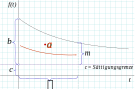
\includegraphics[width=13cm]{allg/funktionen/img/saettigung/saettigungskurveDown.png}}
\end{center}

Die Grundform eines begrenzten Zerfalls ist ein normaler
exponentieller Zerfall ($y=a^{t}$, $0<a<1$), der in $y$-Richtung um eine Sättigungsgrenze $c$ verschoben ist:

\begin{definition}{beschränkter Zerfall}{}
$$f(t) = c + b\cdot{}a^{\frac{t}{\tau}}$$
\end{definition}

Dabei ist:
\begin{itemize}
  \item $c+b = f(0) = y$-Achsenabschnitt = Startwert
	\item $c$: Die Sättigungsgrenze\index{Sättigungsgrenze} (Sättigungswert). Dies ist die Annäherungskonstante oder der \textbf{Asymtote}nwert\index{Asymptote}: Tiefer kann die Funktion nicht fallen.

	\item $m$:
    Sättigungs\textbf{differenz}\index{Sättigungsdifferenz}\index{Differenz!zur
      Sättigung}. Wie viel fehlt, bis zur
    Sättigungsgrenze: $m = f(t) - c$. Die Sättigungs\textbf{differenz} nimmt exponentiell ab.
	\item $b$: Die \textbf{Abweichung} zu $c$ zum Zeitpunkt $t=0$. Der
    Anfangswert ist somit $f(0) = c + b$; mit anderen Worten: $b$ ist das
    \textbf{Sättigungsdifferenz} zum Zeitpunkt $t_0 = 0$.

    \item $a=\frac{m}{b}=\frac{f(\tau)-c}{f(0)-c}$: Der Faktor der Veränderung der
      Sättigung\textbf{differenz}.
\end{itemize}

\subsection*{Aufgaben}
\GESOAadBMTA{359}{35. (Kuchen) und 36. (Ovomaltine)}
\olatLinkGESOKompendium{3.4.2}{33}{48. (Achtung: Das
  Kompendium verwendet andere Buchstaben: Das dortige $a$ ist unser $b$.)}

\GESO{\olatLinkArbeitsblatt{Exponentialfunktionen}{https://olat.bbw.ch/auth/RepositoryEntry/572162163/CourseNode/106029175831971}{Kap. 3.1:
    Sättigung: Begrenzter Zerfall}}
\TALS{\olatLinkArbeitsblatt{Exponentialfunktionen}{https://olat.bbw.ch/auth/RepositoryEntry/572162090/CourseNode/106029175777725}{Kap. 3.:
    Sättigung: Begrenzter Zerfall}}
\newpage


\subsection{Sättigung (begrenztes Wachstum)}\index{Sättigung}\index{begrenztes Wachstum}\index{Wachstum!begrenztes}
\subsubsection{Einstiegsbeispiel 1: Eistee wärmen}
Das Aufwärmen von Eistee von $5\degre$ Kühlschranktemperatur auf $20\degre$ Zimmertemperatur ist ein klassisches «Begrenztes Wachstum» (mit gespiegelter Exponentialfunktion).

\TNT{5.2}{Skizze}

\subsubsection{Einstiegsbeispiel 2: Batterie laden}
\begin{center}
\raisebox{-1cm}{
\includegraphics[width=8cm]{allg/funktionen/img/saettigung/batterien.png}}
\end{center}

Eine 9V-Batterie ist etwas mehr als zur Hälfte entladen und enthält nun eine
Restspannung von 4V.

Wenn wir 9V an die Batterie anlegen, so wird die Batterie geladen.

Die Batterie lädt sich umso rascher, je \textit{leerer} sie ist.

Die Batterie lädt sich umso langsamer, je \textit{voller} sie ist.


\newpage

\subsubsection{Allgemeine Form von Sättigungsprozessen}

\begin{center}
\raisebox{-1cm}{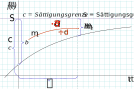
\includegraphics[width=13cm]{allg/funktionen/img/saettigung/saettigungskurve.png}}
\end{center}

Die Grundform des begrenzten Wachstums ist ein exponentieller Zerfall\totalref{zerfallsfunktion},
der an der $x$-Achse gespiegelt und in $y$-Richtung
verschoben ist:

\begin{definition}{Sättigung}{}
$$f(t) =c - b\cdot{} a^{\frac{t}{\tau}}$$
\end{definition}

Die Variable haben die folgenden Bedeutungen:

\begin{itemize}
	\item $c$: Sättigungsgrenze. Dies ist die Annäherungskonstante oder der Asymtotenwert. Höher kann die Funktion nicht steigen.

	\item $m$ ist die
    Sättigungsdifferenz\index{Sättigungsdifferenz}\index{Differenz!zur
    Sättigung}. Wie viel fehlt, bis zur
    Sättigungsgrenze: $m = c - f(t)$. Auch hier nimmt die Sättigungs\textbf{differenz} exponentiell ab.
	\item $b$: Die Abweichung des Funktionsgraphen zu $S$ zum Zeitpunkt $t=0$. Der
    Anfangswert ist somit $f(0) = c - b$.
\item $a=\frac{m}{b}=\frac{c-f(\tau)}{c-f(0)}$ Faktor der Veränderung
  der Sättigungs\textbf{differenz}.
\end{itemize}


\subsubsection{Bemerkungen}
\begin{bemerkung}{}{}
  Für die Sättigungsdifferenz gilt:

\TNT{4}{$$m = m(t) = c - f(t) = c - \left(c-b\cdot{}a^{\frac{t}{\tau}}\right) = + b\cdot{}a^{\frac{t}{\tau}}$$

und somit:

$$m_0 = m(0) = b\cdot{}a^0 = b$$}%% END TNT
\end{bemerkung}

\TRAINER{ Bemerkung (Trainer/mündlich):
  
Das $a$ kann aus zwei \textbf{beliebigen} Sättigungsdifferenz-Werten berechnet werden (die um die
Zeitdifferenz $\tau$ auseinander liegen):
$$\frac{m_2}{m_1} = \frac{b\cdot{}a^{\frac{t_2}{\tau}}}{b\cdot{}
  a^{\frac{t_1}{\tau}}} = a^{\frac{t_2}{\tau}} : a^{\frac{t_1}{\tau}} =
a^{\frac{t_2-t_1}{\tau}} = a^{\frac{\tau}{\tau}} = a$$%% 
}%% END Trainer


\begin{bemerkung}{}{}
Meistens ist $m_0$ zum Zeitpunkt $t=0$ bekannt und somit ist $b=m_0$. Es reicht, die Messung zum Zeitpunkt $t_0$ und zu einem weiteren Zeitpunkt durchzuführen. Wenn zusätzlich die Sättigungsgrenze $c$ bekannt ist, kann die Funktion $f$ komplett bestimmt werden.
\end{bemerkung} 

\newpage

\subsection{Referenzaufgaben}

\subsubsection{Berechnung am Batterie-Beispiel}\index{Batterie}
Eine Batterie weist zum Zeitpunkt $t_0$ vier Volt auf. Nach sechs Stunden am Ladegerät zeigt die Messung sieben Volt. Wir wissen, dass die Sättigungsgrenze (Ladespannung) bei neun Volt liegt.

Zeichnen Sie die gegebenen Größen in ein Koordinatensystem ein und markieren Sie bei neun Volt eine horizontale Beschränkungslinie (\zB 1V = 1 Häus'chen in $y$-Richtung; 1h = 1 Häus'chen in $x$-Richtung).

\noTRAINER{\mmPapier{8.8}}
\TRAINER{\bbwCenterGraphic{15cm}{allg/funktionen/img/saettigung/batterieFct.png}}

\textbf{Frage 1}: Wie lautet die Formel $f(t) = ...$ der Sättigungskurve?

\noTRAINER{$c = ..........................$}
\TRAINER{$c = \textrm{ Sättigungsgrenze } = 9 [\textrm{V}]$}

\noTRAINER{$b = ..........................$}
\TRAINER{$b = m_0 = c-f(0) = 9 - 4 = 5$}

\noTRAINER{$m =  ..........................$}
\TRAINER{$m = m_1 = c-f(\tau) = 9 - 7 = 2$}

\noTRAINER{$a = .........................$}
\TRAINER{$a=\frac{m}{b} = \frac{m_1}{m_0} = \frac{2}{5} = 0.4$}

\noTRAINER{$\tau = .........................$}
\TRAINER{$\tau = 6$ ($e_x$ = eine Stunde)}


\noTRAINER{$f(t) = c - b\cdot{}a^{\frac{t}{\tau}} = ..... - .....\cdot{}(.....)^{\frac{-t}{.....}}$}
\TRAINER{$f(t) = c - b\cdot{}a^{\frac{t}{\tau}} = 9 - 5\cdot{}(\frac{2}{5})^{\frac{t}{6}}$}

\TRAINER{Die Kontrollen für $t=0$ und $t=6$ sind mit dem Stehenlassen von $a$ als Bruch nun sehr einfach.}
\newpage

\textbf{Frage 2}: Wann wird die Batterie zu 99\% geladen sein?

\TNTeop{99\% von 9V = 8.91 V

  Somit ist $t$ gesucht mit $f(t) = 9 - 5\cdot{}\left(\frac25\right)^{\frac{t}{6}} = 8.91$

  (beidseitig -9 und Vorzeichen drehen und dann durch 5 teilen, so folgt...)

  $$(0.4)^{\frac{t}{6}} = (9-8.91) : 5 = 0.09 : 5 = 0.018$$

  Definition Logarithmus:

  $$\frac{t}6 = \log_{0.4}(0.018) \approx 26.3 $$

  Nach ca. 26 - 27 Stunden ist die Batterie zu 99\% geladen.
}
\newpage

\subsubsection{Referenzaufgabe Sättigung: Pneu}\index{Reifen}\index{Pneu}

Ein Reifen (Pneu) ist anfänglich ganz leer und enthält «nur» 1 atm, nämlich den
Druck der Umgebung. (1 atm = atmosphärischer Druck = technische Atmosphäre) 

Der Reifen wird aufgepumpt mit einer Druckpumpe, die maximal 2 atm
leisten
kann. Mit 2 atm ist hier gemeint: 2 at mehr als der
Umgebungsdruck. Somit könnte der Pneu bis auf maximal 3 atm aufgepumpt
werden (= Sättigungsgrenze).

Um den Reifen optimal zu füllen, wird er auf 2 atm aufgepumpt (1 atm
über dem Umgebungsluftdruck).

Die Pumpe schafft in den ersten 10 Sekunden den Druck von 1 atm auf 1.2
atm (= 0.2 atm über Normaldruck) aufzupumpen.

Nach wie vielen Sekunden muss gestoppt werden, damit der Reifen
optimal gepumpt ist?

\TNTeop{Die Sättigungsdifferenz schwindet von $m_1=3-1=2$ bis $m_2=3-1.2=1.8$
innerhalb der ersten $10s = \tau$. Die Sättigungsgrenze liegt bei
$S=3$. Unsere (Exponential)basis $a$ ist somit $1.8 / 2$, was uns
liefert:
$$f(t) = 3 - 2\cdot{}\left(\frac{1.8}{2}\right)^\frac{t}{10}$$
Somit ist das Optimum bei $2 = 3-
2\cdot{}\left(\frac{1.8}{2}\right)^\frac{t}{10}$ erreicht, also bei
etwa 65.8 Sekunden.
}
\newpage

\GESO{\subsection*{Aufgaben}}
\GESOAadBMTA{358}{34. (Eistee)}
\olatLinkGESOKompendium{3.4.2}{32ff}{49. - 51. (Bem.: Das
  Kompendium gibt die Funktionsterme bereits an und verwendet als
  Basis i.\,d.\,R. die Eulersche Konstante $e\approx{} 2.71828$)}

\GESO{\olatLinkArbeitsblatt{Exponentialfunktionen}{https://olat.bbw.ch/auth/RepositoryEntry/572162163/CourseNode/106029175831971}{Kap. 3.1:
    Begrenztes Wachstum}}%% END GESO
\TALS{\olatLinkArbeitsblatt{Exponentialfunktionen}{https://olat.bbw.ch/auth/RepositoryEntry/572162090/CourseNode/106029175777725}{Kap. 3.1:
    Begrenztes Wachstum}}%% END TALS

\newpage

\subsection{Zusammenfassung der Prozesse}
\vspace{8mm}
\begin{center}\textbf{Wachstum und Zerfall}\end{center}

\TNT{8.8}{\bbwCenterGraphic{18cm}{allg/funktionen/img/zusammenfassung_exp/wachstum_zerfall.png}

  bzw.
  $$f(t) = G_0 \cdot{} \e^{qt}; q=  \frac{\ln(a)}\tau  \,\,\,\,\,\,\,\,\, f(t) = G_0 \cdot{} \e^{-qt}; q  = \frac{-\ln(a)}\tau$$
}%% END TNT

\vspace{8mm}
\begin{center}\textbf{Sättigung}\end{center}

\TNTeop{\bbwCenterGraphic{18cm}{allg/funktionen/img/zusammenfassung_exp/saettigung.png}

    bzw.
     $$f(t) = S + (G_0-S) \cdot{} \e^{q\cdot{}t}; q=    \frac{\ln(a)}\tau     \,\,\,\,\,\,\,\,\, f(t) = S + (S - G_0) \cdot{} \e^{-q\cdot{}t}; q  = \frac{-\ln(a)}\tau$$

Hier ist Platz für das Video/die Videos zur den getanzten
Funktionen (S. OLAT/Wiki).
}%% END TNTeop

\newpage

\TALS{
  \subsection*{Aufgaben}
  \olatLinkTALSStrukturaufgabenSPF{Basiskenntnisse Funktionen Teil
    1}{5}{4., 5., 8. und 9.}
  \olatLinkTALSStrukturaufgabenSPF{Basiskenntnisse Funktionen Teil
    2}{14}{45., 47. und 49.}
}%% END TALS
\newpage


%% Gleichungen I
%%%%%%%%%%%%%%%55
%% Funktionen II GESO Metapackage
\part{Funktionen II}\index{Funktionen!II|textbf}
\renewcommand{\bbwPartID}{FCT2}
\section{Potenzfunktionen}\index{Funktion!Potenzfunktionen}\index{Potenzfunktionen}
\sectuntertitel{Funktionen hoch drei!}

\subsection*{Lernziele}

\begin{itemize}
\item Definition Ganzzahlige Potenzfunktion
\item Graphische Darstellung
\end{itemize}
\newpage


\subsection{Einstieg}

%%%%%%%%%%%%%%%%%%%%%%%%%%%%%%%%%%%%%%%%%%%%%%%%%%%%%%%%%%%%%%%%%
\subsubsection{Beispiel: Rationale Funktion\GESO{ (optional)}}

Betrachten wir einmal die Funktion $f: y = 0.1x^3 + x^2 + 2x + 3 - x^{-1}$ \zB mit Geogebra (\texttt{www.geogebra.org}).

\bbwGraph{-10}{4}{-7}{8}{%
  \bbwFunc{0.1*\x*\x*\x + \x*\x + 2*\x + 3 -1/\x}{-8.5:-0.2}
  \bbwFunc{0.1*\x*\x*\x + \x*\x + 2*\x + 3 -1/\x}{0.1:1.5}
}%%


Polynomfunktionen und rationale Funktionen sind «\textit{weiche}» Funktionen, die jedoch \textbf{Asymptoten}\index{Asymptote} (hier bei $x=0$) aufweisen können.
Ebenso sind die Extremwerte (lokale Maxima und Minima)\TALS{ wie auch die Wendepunkte} charakteristische Stellen und oft Gegenstand der Untersuchung.
Wir beschränken uns \TALS{vorerst }auf Funktionen der Art $f: y=a\cdot{}x^z$
mit $z \in \mathbb{Z}\backslash\{0\}$\TRAINER{ $z=0$ ist eine
  Proportionalität und somit hier unspannend}.

\newpage



\subsubsection{\GESO{Beispiel}\TALS{Repetition}: Reinquadratische Funktion}\index{quadratische Funktion}\index{Funktion!quadratische}

Zeichnen Sie den Graphen der Funktion $f: y= \frac16 x^2$:

\bbwGraph{-7}{7}{-1}{6.5}{%%
  \TRAINER{
    \bbwFunc{\x*\x/6}{-6:6}
  }
}%%

\begin{definition}{Reinquadratische Funktion}{}
Die Funktion

$f: y = a\cdot{}x^2$

heißt \textbf{Parabel zweiter Ordnung} oder rein-quadratische Funktion.
\end{definition}


\TALS{
\begin{bemerkung}{}{}
Eine allgemeine quadratische Funktion besitzt auch noch einen linearen ($bx$) und einen konstanten ($c$) Anteil. Die allgemeine quadratische Funktion hat die Form

$$f: y= ax^2 + bx + c$$
\end{bemerkung}
}%% END TALS

\TALS{Beispiele zu allgemeinen quadratischen Funktionen finden sie im
  Buch \cite{marthaler21alg} ab Seite 260 insb. im Bild zu Aufg. 4 auf
  Seite 273.}%% END TALS

\newpage

\subsection{Parabel}\index{Parabel}

Zeichnen Sie $y = \frac{1}{16}x^4$ im Bereich $[-3; 3]$ indem Sie für jeden 0.5-er $x$-Wert das zugehörige $y$ berechnen:

\bbwGraph{-4}{4}{-1}{6.5}{%%
  \TRAINER{\bbwFunc{\x*\x*\x*\x/16}{-3:3}}
}%%


\begin{definition}{Parabel}{definition_parabel}
  Ist $n\in \mathbb{N}_{\ge 2}$, so wird der Graph der Potenzfunktion
  $$x\mapsto a\cdot{}x^n$$
  \textbf{Parabel} $n$-ter Ordnung genannt.
\end{definition}

\TALS{%%
\begin{bemerkung}{Potenzfunktion}{definition_potenzfunktion}
  Eine Funktion der Art
$$f: y=a\cdot{}x^r$$
  mit $r \in \mathbb{R}\backslash\{0\}$ heißt \textbf{Potenzfunktion}.
\end{bemerkung}

\begin{bemerkung}{Polynomfunktionen}{}
  Funktionen, deren Funktionsterm ein Polynom bilden werden
  \textbf{Polynomfunktionen} genannt:
  $$f: y=a_n\cdot{}x^n + a_{n-1}\cdot{}x^{n-1} + a_{n-2}\cdot{}x^{n-2} + ... + a_2\cdot{}x^2 + a_1 \cdot{} x + a_0 $$
\end{bemerkung}
%
}%% END TALS


\newpage
\subsection*{Aufgaben}
\aufgabenFarbe{Zeichnen Sie die Parabeln $$y=f(x) = x^n$$ für $n = 2$,
  $n=3$, $n=4$, $n=5$ und $n=6$ mit \texttt{geogebra.org}.
\\
Was fällt auf?}
%%\GESOAadBMTA{303ff}{1. (nur $n=3$ und $n=5$), 2. (nur $n=4$ und $n=6$)}

\TNTeop{}

\newpage

\subsubsection{Anwendung (optional)}
Boltzmannsches T-hoch-vier-Gesetz\index{Boltzmann!$T^4$-Gesetz}

\leserluft{}

Die Funktion $P(T) = \sigma\cdot\varepsilon\cdot
  A\cdot{}T^4$ beschreibt, welche Strahlungsleistung $P$ ein Körper der
  Oberfläche $A$ (in $ \text{m}^2$) bei Temperatur $T$ (in Kelvin) aussendet.

  $\sigma$ = Bolzmann Konstante = $5.6\cdot{}10^{-8}$
  
  $\varepsilon$ = Emissionswert

  \small{\texttt{(eg. https://ennologic.com/wp-content/uploads/2018/07/Ultimate-Emissivity-Table.pdf)}}

  \leserluft{}
  
  Rechenbeispiel:

\TNTeop{$T$ = 20 Grad Zimmertemperatur in Kelvin: 293.15;
  Brick (Haus) hat Emissionswert ca. 0.75; Haus Oberfläche $500 \text{m}^2$

  $$P(293.15) \approx 5.6\cdot{}10^{-8} \cdot{} 0.75 \cdot{} 500
  \cdot{} 293.15^4 \approx 155 \text{kW} $$
  Natürlich strahlt eine 20-grädige Umgebungstemperatur gleich viel
  wieder zurück, sodass keine 'Heizkosten' entstehen.

  Heizen wir das Haus nun zwei Grad wärmer, so erhalten wir:
  $$P(295.15) \approx 5.6\cdot{}10^{-8} \cdot{} 0.75 \cdot{} 500
  \cdot{} 295.15^4 \approx 159.4 \text{kW} $$

  Dies entspricht einer Differenz von 4.28 kW für nur zwei Grad wärmer
  im Haus!
  

}%% END TNT
\newpage

Zeichnen Sie des weiteren die Funktion $y = \frac{1}{9}x^3$:

\bbwGraph{-4}{4}{-5}{5}{%%
  \TRAINER{\bbwFunc{\x*\x*\x/9}{-3.5:3.5}}
}%%

\subsubsection{Symmetrien}\index{Symmetrien!von Parabeln}\index{Parabel!Symmetrie}
Was fällt für gerade und ungerade Exponenten auf? Gibt es Spiegelachsen
oder Spiegelpunkte?

\renewcommand{\mmPapier}[1]{\mmPapierZwei{#1}{16.4}}
\begin{tabular}{c|p{8cm}}
  $x^2$ & \vspace{0.1mm}\TNT{0.8}{An der $y$-Achse}\\\hline
  $x^3$ & \vspace{0.1mm}\TNT{0.8}{Am Ursprung $O(0|0)$}\\\hline
  $x^4$ & \vspace{0.1mm}\TNT{0.8}{wie $x^2$}\\\hline
  $x^5$ & \vspace{0.1mm}\TNT{0.8}{wie $x^3$}\\\hline
\end{tabular}
\renewcommand{\mmPapier}[1]{\mmPapierZwei{#1}{17.6}}


\GESO{Eine Zusammenfassung der wichtigsten Eigenschaften von
  Potenzfunktionen finden Sie im Buch \cite{marthaler21alg} Seite 296 oben.}
\newpage

\subsubsection{Referenzaufgabe}

Bestimmen Sie $a$ und $k$ so, dass der Graph von $y = a \cdot{} x^k$
durch die Punkte $P=\left(3 \middle| 1458\right)$ und
$Q=\left(-4\middle|8192\right)$ verläuft.

\TNT{15.2}{ Punkte einsetzen in die Funktionsgleichung:
  \gleichungZZ{1458}{a\cdot{}3^k}{8192}{a\cdot{}(-4)^k}
  Aus der oberen Gleichung das $a$ ermitteln ($a=\frac{1458}{3^k}$)
  (I) und in die zweite
  Gleichung einsetzen: $$8192 = \frac{1458}{3^k} \cdot{} (-4) ^k$$
  Exponent $k$ separieren:
  $$\frac{8192}{1458} = \left(\frac{-4}3\right)^k$$
  Problem: Logarithmen mit negativen Basen (hier $\frac{-4}3$)
  funktionieren nicht!
  
  Weil nun $k$ gerade sein muss, folgt dass $\left(\frac{-4}3\right)^k
  = \left(\frac43\right)^k$. Daraus ergibt sich
  $$\frac{8192}{1458} = \left(\frac{4}3\right)^k \Longrightarrow k =
  \log_{\frac43}\left(\frac{8192}{1458}\right) = 6$$
  Dieses $k$ nun in die Gleichung (I) einsetzen; dies
  liefert
  $$a=\frac{1458}{3^k} = 2.$$
}%% end TRAINER


\subsection*{Aufgaben}
\AadBMTA{305ff}{11. a) b) c), 13. a) c), (optional 17.,)  18.}
%%\TALSAadBMTA{197}{735. (6) (7) und (9) jeweils mit geogebra, 736. a) d),
%%  737. a) c), 739.}
\newpage


\subsection{Translationen}\index{Manipulation!Funktionen}\index{Funktions-Manipulation}\index{Translation!Funktion}
\sectuntertitel{Manipulation an Funktionsgraphen}
(Verschiebung\index{Verschiebung}, Spiegelung\index{Spiegelung},
Streckung\index{Streckung})

\TadBMTA{217}{13.3}
%%\TALSTadBFWA{163}{3}
Betrachten Sie die Funktionen

$$f(x) = a\cdot{}\left(\frac{x\TALS{-d}}b\right)^5\TALS{+c}$$
und
$$g(x) = a\cdot{}\left(\frac{x\TALS{-d}}b\right)^4\TALS{+c}$$

mit Geogebra (\texttt{geogebra.org})
und beschreiben Sie die Effekte der Parameter

$a$: \TRAINER{Streckung in $y$-Richtung. $a$ negativ: Spiegelung an der
$x$-Achse.}

\noTRAINER{\mmPapier{2.4}}

$b$: \TRAINER{Streckung entlang der $x$-Achse. $b$ negativ: Spiegelung
  an der $y$-Achse.}

\noTRAINER{\mmPapier{2.4}}

\TALS{%% nur TALS haben Verschiebungen
  $c$: \TRAINER{Verschiebung entlang der $y$-Achse}

\mmPapier{2.4}
}%% end TALS

\TALS{
$d$: \TRAINER{Verschiebung entlang der $x$-Achse (Verschiebung nach
  rechts verlangt ein negatives $d$.)}

\noTRAINER{  \mmPapier{2.4}}
}%% END TALS

\newpage

\subsubsection{Zusammenfassung der Translationen}


Wir betrachten die verschiedenen geometrischen
Funktions-«Manipulationen» (Abbildungen) am Beispiel {\color{red}$y =f(x) = \frac18 x^3$}.


\newcommand{\graphTranslationMultiColumn}[5]{%
  \multicolumn{3}{|l|}{#1}\\%%
\hline%%
\graphTranslationMultiColumnZ{#2}{#3}{#4}{#5}
}%% end new command \graphTranslationMultiColumn

\newcommand{\graphTranslationMultiColumnZ}[4]{%
\multirow{5}{6cm}{#1} &  & \multirow{2}{*}{\begin{minipage}{.3\textwidth}\raisebox{-8cm}{\includegraphics[width=\linewidth,height=60mm]{allg/funktionen/img/translation/#4}}\end{minipage}}\\[55mm]%%
&\fbox{#2}&\\%%
&&\\%%
&{\color{red}\fbox{#3}}&\\%%
&&\\%%
\hline%%
}%% end new command \graphTranslationMultiColumnZ

\TALS{%% Nur TALS haben Verschiebungen
\begin{tabular}{|p{7cm}|c|c|}%%
\hline%%
\graphTranslationMultiColumn{Verschiebung in $y$-Richtung...}{... um \textbf{zwei} Einheiten nach \textbf{oben}:}{$g(x)=f(x)\textbf{+2}$}{$g(x)=\frac18x^3\textbf{+2}$}{typ1.png}
\graphTranslationMultiColumnZ{... um \textbf{eine} Einheiten nach \textbf{unten}:}{$g(x)=f(x)\textbf{-1}$}{$g(x)=\frac18x^3\textbf{-1}$}{typ2.png}
\end{tabular}%%
}%% end TALS

\begin{tabular}{|p{7cm}|c|c|}%%
\hline%%
\graphTranslationMultiColumn{Spiegelung...}{... an der $x$-Achse:}{$g(x)=-f(x)$}{$g(x)=-\frac18x^3$}{typ3.png}
\graphTranslationMultiColumnZ{... an der $y$-Achse:}{$g(x)=f(-x)$}{$g(x)=\frac18(-x)^3$}{typ4.png}
\end{tabular}%%

\begin{tabular}{|p{7cm}|c|c|}%%
\hline%%
\graphTranslationMultiColumn{Streckung...}{... in $y$-Richtung (von der $x$-Achse aus) um Faktor \textbf{zwei}:}{$g(x)=\textbf{2}\cdot{}f(x)$}{$g(x)=\textbf{2}\cdot{}\frac18x^3$}{typ5.png}
\graphTranslationMultiColumnZ{... in $x$-Richtung (von der $y$-Achse aus) um Faktor \textbf{zwei}:}{$g(x)=f(\frac{1}{\textbf{2}}\cdot{}x)$}{$g(x)=\frac18(\frac{1}{\textbf{2}}\cdot{}x)^3$}{typ6.png}
\end{tabular}%%

\TALS{%% Nur TALS verschieben in x-Richtung
\begin{tabular}{|p{7cm}|c|c|}%%
\hline%%
\graphTranslationMultiColumn{Verschiebung in $x$-Richtung\footnote{Kein prüfungsrelevantes Thema.}...}{... um \textbf{zwei} Einheiten nach \textbf{links}:}{$g(x)=f(x\textbf{+2})$}{$g(x)=\frac18(x\textbf{+2})^3$}{typ7.png}
\graphTranslationMultiColumnZ{... um \textbf{zwei} Einheiten nach \textbf{rechts}:}{$g(x)=f(x\textbf{-2})$}{$g(x)=\frac18(x\textbf{-2})^3$}{typ8.png}
\end{tabular}%%
}%% END TALS
\newpage

\subsection*{Aufgaben}
\GESO{
Skizzieren Sie $-\frac{1}{2}x^3 - 1$ im Bereich $x$ = -2 bis $x$ = +2.

\bbwGraph{-4}{4}{-5}{3}{%%
  \TRAINER{%
    \bbwFunc{-0.5*\x*\x*\x-1}{-2:2}%
  }%%
}%

Vergleichen Sie die neue Funktion mit der Parabel $y=x^3$.

\TNT{5.2}{Die neue Funktion ist an der $y$-Achse gespiegelt, ist um
  50\% gestaucht ($y$-Richtung) und ist um eine Einheit nach unten
  ($x$-Richtung) verschoben worden.}
}%% END GESO

\AadBMTA{304ff}{5. a) c) d) e), 9. a) d) e)}

 
\TALS{
  \aufgabenFarbe{Zeichnen Sie mit \texttt{geogebra.org} die Funktion
    $f(x) = \frac1{10}(x^3 - 3x^2 + 3)$
    \\
    Definieren Sie anschließend die Funktion $$g(x) = a\cdot{}f((x+s)\cdot{}b)+r.$$
\\
    Entscheiden Sie, welche Veränderungen die Parameter $a$, $b$, $r$
    und $s$ bewirken.\\
    Starten Sie mit $a=1$, $b=1$, $r=0$ und $s=0$.
  }%% END Aufgabenfarbe
  \TNT{4}{
    $r$: Verschiebung nach oben\\
    $s$: Verschiebung nach links\\
    $a$: Streckung in $y$-Richtung\\
    $b$: Stauchung in $x$-Richtung
  }%% END TNT
}%% END TALS



%%  OLAT Arbeitsblatt
\GESO{\olatLinkArbeitsblatt{Positive Potenzfunktionen zuordnen}{https://olat.bbw.ch/auth/RepositoryEntry/572162163/CourseNode/104752086007823}{(alle Beispiele)}}%% END olatLinkArbeitsblatt
\TALS{\olatLinkArbeitsblatt{Positive Potenzfunktionen zuordnen}{https://olat.bbw.ch/auth/RepositoryEntry/572162090/CourseNode/105597875231723}{(alle Beispiele)}}%% END olatLinkArbeitsblatt


\olatLinkTALSStrukturaufgabenSPF{Teil 2}{15ff}{48. und 51.}
%%\TALS{\aufgabenFarbe{Strukturaufgaben SPF Teil 2: Taschenrechner: S. 15ff:  Aufg. 48. und 51.}%% END Aufgabenfarbe
%%}%% END TALS

%%\TALSAadBMTA{197 ff.}{739., 743. c), 745. c), 738.*}

\olatLinkGESOKompendium{3.3.1.}{26}{28., 29.}
\newpage



%%%%%%%%%%%%%%%%%%%%%%%%%%%%%%%%%%%%%%%%%%%%%%%%%%%%%%%%%%%%%%%%%%%%%%%%%%%%%%%%%%%
\subsection{Hyperbel}\index{Hyperbel (negative Exponenten)}

(«Hyperbel» Griechisch = «über das Ziel hinaus werfen»)


Zur Erinnerung:
\begin{multicols}{2}
\begin{itemize}
	\item $x^{-1} = \frac{1}{x}$
	\item $x^{-2} = \frac{1}{x^2}$
	\item $x^{-3} = \frac{1}{x^3}$
	\item $x^{-4} = \frac{1}{x^4}$
	\item $x^{-5} = \frac{1}{x^5}$
  \item ...
\end{itemize}
\end{multicols}

Zeichnen Sie die Funktion $f: y = x^{-1}$ im Definitinosbereich
$\DefinitionsMenge{} = [-5;5]\TRAINER{\backslash \{0\}}\noTRAINER{......}$

\bbwGraph{-6}{6}{-3}{3}{%%
  \TRAINER{\bbwFunc{1/\x}{-5:-0.3}}
  \TRAINER{\bbwFunc{1/\x}{0.3:5}}

}%%

\newpage


Zeichnen Sie zusätzlich Funktion $f: y = x^{-2}$ im Definitionsbereich $[-5;5]$:

\bbwGraph{-6}{6}{-5}{5}{%%
  % x^-2
  \TRAINER{\bbwFuncC{1/(\x * \x)}{-5:-0.447}{green}}%% 0.447 = 1/sqrt (5)
  \TRAINER{\bbwFuncC{1/(\x * \x)}{0.447:5}{green}}
  \TRAINER{\bbwLetter{2.5,0.5}{x^{-2}}{green}}
  \TRAINER{\bbwLetter{-1.5,1}{x^{-2}}{green}}

  %x^-3
%  \TRAINER{\bbwFuncC{1/(\x * \x * \x)}{-5:-0.584}{blue}}
%  \TRAINER{\bbwFuncC{1/(\x * \x * \x)}{0.584:5}{blue}}
%  \TRAINER{\bbwLetter{0.8,0.3}{x^{-3}}{blue}}
%  \TRAINER{\bbwLetter{-1.2,-3.8}{x^{-3}}{blue}}
%  \TRAINER{\bbwLetter{1.2,4.5}{x^{-3}}{blue}}

}%%

\begin{definition}{Hyperbel}{definition_hyperbel}
  Der Graph einer Potenzfunktion $$f: y=ax^z$$
  mit $z \in \{-1, -2, -3, -4, ...\}$ heißt
\textbf{Hyperbel}\index{Hyperbel} der Ordnung $z$.
\end{definition}

Der Definitionsbereich von Hyperbeln entspricht dem Definitionsbereich
des Funktionsterms. Merke: Es darf nicht durch Null geteilt werden:

$$x^{-5} = \frac{1}{x^5} \Longrightarrow \DefinitionsMenge{} = \mathbb{R} \backslash \{0\}$$


\subsection*{Aufgaben}
\AadBMTA{306ff}{19. Zeichnung mit geogebra.org, 20.
  Zeichnung mit geogebra.org}
%%\TALSAadBMTA{205}{771. a) c) d) e) g) h) j)}


\newpage

\subsubsection{Charakteristiken}
\textbf{Spiegelungen:}\\

Welche Funktionen $x$, $x^{-1}$, $x^{-2}$, $x^{-3}$ sind an welchen Achsen bzw. Punkten gespiegelt?

\renewcommand{\mmPapier}[1]{\mmPapierZwei{#1}{16.0}}
\begin{tabular}{c|p{10cm}}
  $x^{-1}$ &  \TNT{0.8}{Am Ursprung $O(0|0)$ : Punktspiegelung}\\
  \hline
  $x^{-2}$ &  \TNT{0.8}{An der $y$-Achse: Achsensymmetrie}\\
  \hline
  $x^{-3}$ &  \TNT{0.8}{Am Ursprung $O(0|0)$: Punktspiegelung}\\
  \hline
  $x^{-4}$ &  \TNT{0.8}{An der $y$-Achse: Achsensymmetrie}\\
  \hline  
\end{tabular}
\renewcommand{\mmPapier}[1]{\mmPapierZwei{#1}{17.6}}


\paragraph{Definitions- und Wertebereiche:}

Geben Sie für die obigen Funktionen an, was ihr Definitions- bzw. Wertebereich ist\footnote{Grundmenge ist $\mathbb{R}$.}:

\begin{tabular}{c|c|c}
Funktionsterm & Definitionsbereich $\DefinitionsMenge{}$& Wertebereich $\Wertebereich{}$\\ \hline
  $x^{-1}$ & \TRAINER{$\mathbb{R}\backslash\{0\}$} &  \TRAINER{$\mathbb{R}\backslash\{0\}$}\\ \hline
  $x^{-2}$ & \TRAINER{$\mathbb{R}\backslash\{0\}$} &  \TRAINER{$\mathbb{R}^{+}\backslash\{0\}$}\\ \hline
  $x^{-3}$ & \TRAINER{$\mathbb{R}\backslash\{0\}$} &  \TRAINER{$\mathbb{R}\backslash\{0\}$}\\ \hline
  $x^{-4}$ & \TRAINER{$\mathbb{R}\backslash\{0\}$} &  \TRAINER{$\mathbb{R}^{+}\backslash\{0\}$}\\ \hline
\end{tabular}


\GESO{\subsection*{Aufgaben}}
\olatLinkGESOKompendium{3.3}{26}{28. bis 31.}
\GESO{\aufgabenFarbe{Aufgabe der Nullserie 2 (zweite Nullserie): Aufg. 7 auf Seite 3}}
\GESO{\aufgabenFarbe{Maturaprüfung 2016, Aufg. 8 (Graphen zuordnen)}}

\newpage

\newpage

%%%%%%%%%%%%%%%%%%%%%%%%%%%%%%%%%%%%%%%%%%%%%%%%%%%%%%%%%%%%%%%%%%%%%%%%%%%%%%%%%%%

\subsection{Zusammenfassungen und Überblick}\index{Potenzfunktionen!Überblick}

$$y = a\cdot{}x^z$$

$z$ gerade: Gespiegelt an der $y$-Achse

$z$ ungerade: Gespiegelt am Ursprung $O=(0|0)$

Ist ${\color{ForestGreen}a>0}$\TRAINER{ (grün in der Graphik)}, so sind Graphen mit
geraden Exponenten nach oben geöffnet bzw. mit ungeraden Exponenten im
Quadranten I und III.

Ist ${\color{red}a<0}$\TRAINER{ (rot/orange in der Graphik)}, so sind Graphen mit
geraden Exponenten nach unten geöffnet bzw. mit ungeraden Exponenten
im Quadranten II und IV.


\TRAINER{%
  \includegraphics[width=8.5cm]{allg/funktionen/img/potenzfct/potenzFunktionenGerade.png}\hfill{}\includegraphics[width=8.5cm]{allg/funktionen/img/potenzfct/potenzFunktionenUngerade.png}
}%% END Trainer
\noTRAINER{%
  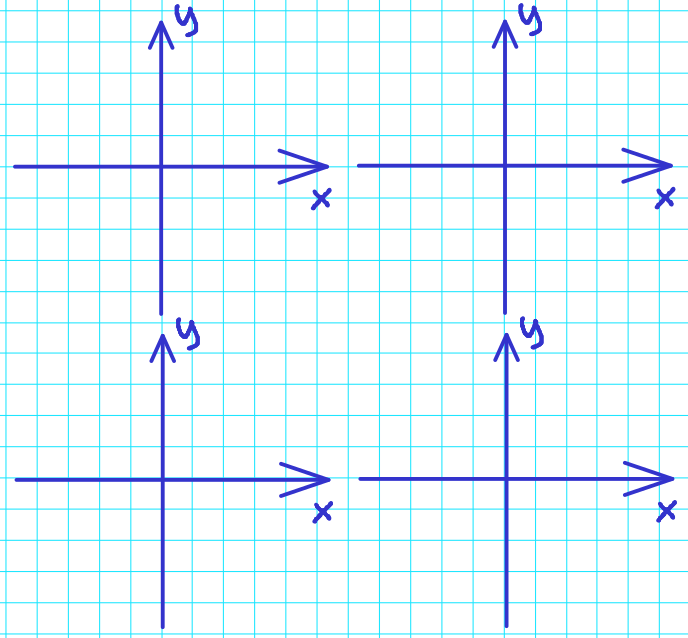
\includegraphics[width=8.5cm]{allg/funktionen/img/potenzfct/potenzFunktionenLeer.png}\hfill{}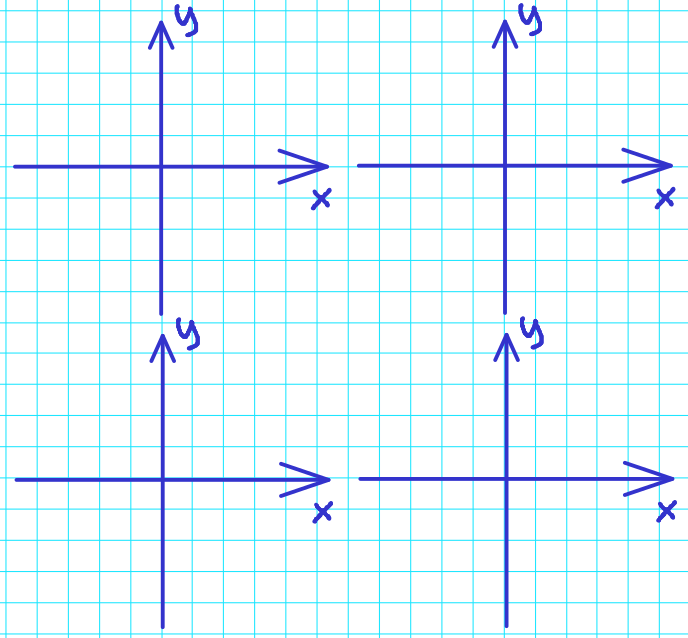
\includegraphics[width=8.5cm]{allg/funktionen/img/potenzfct/potenzFunktionenLeer.png}
}%% END Trainer


\subsection*{Aufgaben}
\AadBMTA{307}{25. b) c), 26. a)\TALS{ b)}, 27. b) c)\TALS{, 33*}}

\newpage


\newpage
\newpage
%%
%% 2019 07 04 Ph. G. Freimann
%%

\section{Exponentialfunktionen}\index{Funktion!Exponentialfunktion}\index{Exponentialfunktionen}
\sectuntertitel{Go viral!}
%%%%%%%%%%%%%%%%%%%%%%%%%%%%%%%%%%%%%%%%%%%%%%%%%%%%%%%%%%%%%%%%%%%%%%%%%%%%%%%%%
\subsection*{Lernziele}

\begin{itemize}
\item Definition Exponentialfunktion
\item Koeffizienten interpretieren
\item Graph: Symmetrien, Polstellen, Asymptoten, Schnittpunkte mit
  Achsen
  \item Basiswechsel
\end{itemize}

\TadBMTA{322}{19}
%%\TALS{(\cite{frommenwiler17alg} S.215 (Kap. 3.10))}
%%\GESO{(\cite{marthaler21alg}       S.322 (Kap. 19))}
\newpage

\subsection{Aussehen von Exponetialfunktionen}


Zeichnen Sie $f: y=2^x$ und $g: y=1.4^x$ ins selbe Koordinatensystem:


\bbwGraph{-5}{5}{-1}{5}{
\TRAINER{  \bbwFuncC{pow(2.0,\x)}{-3.5:2.1}{blue}
  \bbwFuncC{pow(1.4,\x)}{-3.5:3}{green}
  \bbwLetter{1,3}{$f$}{blue}
  \bbwLetter{2.5,2}{$g$}{green}
}%% end TRAINER
}%% end graph

\begin{definition}{Exponentialfunktion}{}\index{Exponentialfunktionen!Definition}
  Eine Funktion der Form $$f(x): x \mapsto a^x$$
  bzw. $$y = a^x$$
  mit $a\in \mathbb{R}^{+}\backslash\{1\}$ heißt \textbf{Exponentialfunktion}.
\end{definition}


\begin{bemerkung}{Zunahmefaktor}{}\index{Zunahmefaktor|textbf}
Der Parameter $a$ gibt den Wachstumsfaktor pro Zeiteinheit $e_x$ an.
\end{bemerkung}


\subsubsection*{Aufgaben}
\GESO{\olatLinkArbeitsblatt{Exponentialfunktionen}{https://olat.bms-w.ch/auth/RepositoryEntry/6029794/CourseNode/106029175831971}{Kap. 1.2:
    Einfache Wachstumsprozesse: Aufgaben 4. bis 6.}}
\TALS{\olatLinkArbeitsblatt{Exponentialfunktionen}{https://olat.bms-w.ch/auth/RepositoryEntry/6029786/CourseNode/106029175777725}{Kap. 1.2:
    Einfache Wachstumsprozesse: Aufgaben 4. bis 6.}}

\newpage

\subsection{Formen der Darstellung}
Zeichnen Sie die Funktionen $f: y=2^x$, $g: y=2^{-x}$ und $h: y=\left(\frac12\right)^x$ in dasselbe Koordinatensystem:

\bbwGraph{-6}{6}{-1}{5}{
  \TRAINER{\bbwFuncC{exp(0.69314718*\x)}{-6:2}{blue}}
  \TRAINER{\bbwFuncC{exp(-0.69314718*\x)}{-2:6}{red} }
  \TRAINER{\bbwLetter{1.5,4}{2^x}{blue}}
  \TRAINER{\bbwLetter{-5,4}{g(x)=2^{-x}=\left(\frac{1}{2}\right)^x=h(x)}{red}}
}

Bemerkung: \TRAINER{$$2^{-x} = \frac1{2^x} = \frac{1^x}{2^x}= \left(\frac12\right)^x$$}
\newpage



\subsubsection{Umkehrung (Optional)}
Um aus einem Wachstum einen Zerfall zu modellieren können wir entweder
die Zeitachse umdrehen oder den Kehrwert der Basis verwenden.
umgedreht werden:

Mit $d := \frac1a $ gilt:

\begin{center}
  \fbox{$a^{+t} = \left(\frac1a\right)^{-t} = d^{-t} $}
\end{center}

\newpage

\newpage

\subsection{Verschiebung und Streckung \GESO{(optional)}}

Eine Verschiebung der Exponentialfunktion $y=b\cdot{}a^x$ in der Zeit ($x$-Richtung) kann auch in Form einer Veränderung der Startfaktors $b$ umgeschrieben werden.

Verschieben wir \zB $$y=2^x$$ um fünf Einheiten nach rechts, so liest sich die neue Funktionsgleichung wie folgt:
$$y=2^{x-5}.$$

(Zeichnen Sie in \texttt{geogebra.org} a) $y=2^x$ und b) $y=2^{x-5}$.)

Dies kann jedoch auch umgeschrieben werden:

$$2^{x-5} = 2^x \cdot{} 2^{-5} = 2^{-5} \cdot{} 2^x = \frac{1}{2^5} \cdot{} 2^x =
\frac{1}{32}\cdot{}2^x$$

\bbwCenterGraphic{8cm}{allg/funktionen/img/exp/verschiebung_gleich_streckung.png}
Bildlegende: Eine Verschiebung ($x$-Richtung) der Exponentialfunktion entspricht einer Stauchung ($y$-Richtung) der selben Exponentialfunktion.

\TALS{Es gilt hier $$a^{x-b}=\frac{a^x}{k}$$ mit
$k=a^b$ und mit $b=\log_a(k)$.}

\newpage


\subsection{Punkte einsetzen\GESO{ (optional)}}
Wie bei den linearen Funktionen oder bei den Potenzfunktionen können auch Exponentialfunktionen gefunden werden, wenn bereits Punkte auf dem Graphen bekannt sind:

\textbf{Referenzaufgabe}

Finden Sie die Parameter $a$ und $b$ der Exponentialfunktion
$$f: y=b\cdot{}a^x$$
wenn Sie wissen, dass die Funktion durch die Punkte $P=(2|4)$ und $Q=(-1|2)$ verläuft:

\TNTeop{
  In Gleichung einsetzen:

  \gleichungZZ{4}{b\cdot{}a^2}{2}{b\cdot{}a^{-1}}

  Einsetzverfahren: Zum Beispiel aus der zweiten Gleichung das $b$ ermitteln...
  $$b = 2 a (III)$$
  ... und in die erste Gleichung einsetzen:

$$4 = 2a\cdot{} a^2$$
  $$2 = a^3$$
  $$a=\sqrt[3]{2}$$
  In (III) einsetzen:

  $$b = 2 \sqrt[3]{2}$$

  Ergo: $$f(x) = b\cdot{}a^x = 2\cdot{}\sqrt[3]{2} \cdot{} \left(\sqrt[3]2\right)^x \approx 2.5198 \cdot{} 1.2599^x$$
}

\subsection*{Aufgaben}
%%\AadBMTA{334}{10. a) b)\TALS{ e)}\GESO{ f)}}
\GESO{\olatLinkArbeitsblatt{Exponentialfunktionen}{https://olat.bms-w.ch/auth/RepositoryEntry/6029794/CourseNode/106029175831971}{Kap. 2.1: E-Funktion / Punkte-Aufgaben Aufg 26. a) b) ($e^{qt}$ optional) und Aufg. 27.}}
\TALS{\olatLinkArbeitsblatt{Exponentialfunktionen}{https://olat.bms-w.ch/auth/RepositoryEntry/6029786/CourseNode/106029175777725}{Kap. 2.1: E-Funktion / Punkte-Aufgaben Aufg 26. a) b) ($e^{qt}$ optional) und Aufg. 27.}}

\AadBMTA{336}{23. d}

\newpage

\newpage
%% 2019 07 04 Ph. G. Freimann
%%

\section{Wachstum und Zerfall}\index{Wachstum}\index{Zerfall}
\sectuntertitel{Sagt ein großer Stift zum kleinen Stift: ``Wachsmalstift!''}

%%%%%%%%%%%%%%%%%%%%%%%%%%%%%%%%%%%%%%%%%%%%%%%%%%%%%%%%%%%%%%%%%%%%%%%%%%%%%%%%%

\TRAINER{
  Video \href{https://www.youtube.com/watch?v=TMaLuks8dxw}{MatheMann}
Wo schneiden sich $x^3$ und $e^x$?}%%
\subsection*{Lernziele}

\begin{itemize}
\item Zinseszins
\item Wachstums-, Zerfallsprozesse
\item Verdoppelungs- und Halbwertszeiten
%%\item Basiswechsel
\end{itemize}

\TadBMTA{342}{20}
%%\TALS{(\cite{frommenwiler17alg} S.221 (Kap. Exponentielles Wachstum))}
%%\TALS{(\cite{frommenwiler17alg} S.223 (Kap. Exponentielle Abnahme))}
%%\TALS{(\cite{frommenwiler17alg} S.225 (Kap. Zinseszins))}
%%\GESO{(\cite{marthaler21alg}       S.342 (Kap. 20))}

\newpage


\subsection{Beispiele}
Bei Wachstumsprozessen sprechen wir dann von einer exponentiellen
Zunahme, wenn die Zunahme pro Zeiteinheit immer proportional zum aktuellen Bestand ist.

\begin{itemize}
\item \Lueckentext{Zinseszins}
\item \Lueckentext{Frequenzen in der temperierten Stimmung
  (Musik). Zunahme der Frequenz pro Halbtonschritt.}
\item \Lueckentext{Keime in der Kuhmilch; Ansteckungsbedingte Krankheitsfälle (\zB viral)}
\item \Lueckentext{Algenbefall in Teichen}
\item \Lueckentext{Generell Populationen: Flechten, Pilze}
\item \Lueckentext{(ungebremstes) Bevölkerungswachstum / bzw. Tierpopulation}
\item \Lueckentext{\dotfill}
\end{itemize}


\GESO{\olatLinkArbeitsblatt{Exponentialfunktionen}{https://olat.bms-w.ch/auth/RepositoryEntry/6029794/CourseNode/106029175831971}{Kap. 1.1:
    Voraussetzungen: Aufgaben 1. bis 3.}}
\TALS{\olatLinkArbeitsblatt{Exponentialfunktionen}{https://olat.bms-w.ch/auth/RepositoryEntry/6029786/CourseNode/106029175777725}{Kap. 1.1:
    Voraussetzungen: Aufgaben 1. bis 3.}}


\newpage

\subsection{Einstiegsbeispiel Taschengeld}

Bei Familie Cash kann man aussuchen, wie sich sein Taschengeld über
die Jahre «vermehrt». Mani wählt Variante A. Bei Varante A erhält man
CHF 1.- im ersten Jahr, CHF 2.- im 2. Jahr, CHF 3.- im 3. Jahr und so
weiter bis zur abgeschlossenen Grundbildung im 13. Jahr CHF 13.-.

Carla wählt Variante B. Bei der Variante B erhält Carla auch CHF 1.-
im ersten Jahr, dann aber jedes Jahr 30\% mehr, als im Vorjahr.

a) Wird Carla vor Ende der Grundbildung jemals mehr als Mani erhalten?

\LoesungsRaumLang{Ja, im 10. Schuljahr}

b) Wer hat über alle Jahre mehr Taschengeld?

\LoesungsRaumLang{Carla wird mehr haben}

c) Skizzieren Sie beide Varianten:

\TRAINER{\bbwCenterGraphic{13cm}{allg/funktionen/img/taschengeldAusgefuellt.png}}
\noTRAINER{\bbwCenterGraphic{16cm}{allg/funktionen/img/taschengeld.png}}

\TRAINER{Optional: Zeige mit Geogebra (\texttt{geogebra.org}) $x^2$ vs. $1.2^x$. Fazit:
  Exponentielles Wachstum überholt jegliche Potenzfunktion.}



\newpage

Zeichnen Sie $f: y=2^x$ und $g: y=1.4^x$ ins selbe Koordinatensystem:


\bbwGraph{-5}{5}{-1}{5}{
\TRAINER{  \bbwFuncC{pow(2.0,\x)}{-3.5:2.1}{blue}
  \bbwFuncC{pow(1.4,\x)}{-3.5:3}{green}
  \bbwLetter{1,3}{$f$}{blue}
  \bbwLetter{2.5,2}{$g$}{green}
}%% end TRAINER
}%% end graph

\begin{definition}{Exponentialfunktion}{}\index{Exponentialfunktionen!Definition}
  Eine Funktion der Form $$f(x): x \mapsto a^x$$
  bzw. $$y = a^x$$
  mit $a\in \mathbb{R}^{+}\backslash\{1\}$ heißt \textbf{Exponentialfunktion}.
\end{definition}


\begin{bemerkung}{Wachstumsfaktor}{}\index{Wachstumsfaktor}
Der Parameter $a$ gibt den Wachstumsfaktor pro Zeiteinheit $e_x$ an.
\end{bemerkung}


\subsubsection*{Aufgaben}
\GESO{\olatLinkArbeitsblatt{Exponentialfunktionen}{https://olat.bms-w.ch/auth/RepositoryEntry/6029794/CourseNode/106029175831971}{Kap. 1.2:
    Einfache Wachstumsprozesse: Aufgaben 4. bis 6.}}
\TALS{\olatLinkArbeitsblatt{Exponentialfunktionen}{https://olat.bms-w.ch/auth/RepositoryEntry/6029786/CourseNode/106029175777725}{Kap. 1.2:
    Einfache Wachstumsprozesse: Aufgaben 4. bis 6.}}


\newpage

\subsection{Exponentieller Zerfall}\label{zerfallsfunktion}
Die Funktion $f(x): x \mapsto y = d^{-x}$ ist eine
Exponentialfunktion, die gegen Null geht.

\bbwFunction{-4}{4}{-1}{8}{exp(-\x)}{-2:4}

\begin{bemerkung}{}{}
Oft wird bei Wachstumsprozessen die Zeitachse auch mit $t$ statt $x$ bezeichnet: $t$ steht für \textit{time}.
\end{bemerkung}

\newpage

\subsubsection{Beispiele}
\begin{itemize}
	\item \Lueckentext{Zinsliche Abschreibungen (\zB Wert eines Autos)}
	\item \Lueckentext{Radioaktiver Zerfall}
	\item \Lueckentext{Lichtintensität in Medium (Gas / Flüssigkeit / Glasfaser), dies gilt vertikal, wie auch horizontal}
	\item \Lueckentext{Atmosphärischer Luftdruck in Metern über Meer}
  \item \Lueckentext{Entladen einer Batterie bzw. eines Kondensators}
  \item \Lueckentext{Sauerstoffkonzentration in Seen (\zB Herbst bei kontinuierlicher Abnahme)}
  \item \Lueckentext{Abnahme des Bierschaums im Glas}
  \item \Lueckentext{Mischen, wie im Sirup-Beispiel\totalref{sirup_beispiel}}
  \item \Lueckentext{«Halbwertszeit des Wissens» ;-)}
  \item \Lueckentext{\dotfill}
\end{itemize}

\newpage



Zeichnen Sie die Funktionen $f: y=2^x$, $g: y=2^{-x}$ und $h: y=\left(\frac12\right)^x$ in dasselbe Koordinatensystem:

\bbwGraph{-6}{6}{-1}{5}{
  \TRAINER{\bbwFuncC{exp(0.69314718*\x)}{-6:2}{blue}}
  \TRAINER{\bbwFuncC{exp(-0.69314718*\x)}{-2:6}{red} }
  \TRAINER{\bbwLetter{1.5,4}{2^x}{blue}}
  \TRAINER{\bbwLetter{-5,4}{g(x)=2^{-x}=\left(\frac{1}{2}\right)^x=h(x)}{red}}
}

Bemerkung: \TRAINER{$$2^{-x} = \frac1{2^x} = \frac{1^x}{2^x}= \left(\frac12\right)^x$$}
\newpage

\subsubsection{Grundform} \index{Exponentieller Prozess! Grundform}
Die Grundform für Zerfallsprozesse lautet:

\begin{definition}{Zerfall}{}\index{Zerfall}
  Die Grundform des exponentiellen Zerfalls wird beschrieben durch die Funktion
$$f(x): x \mapsto a^x$$
  bzw.
  $$y = a^x$$
\end{definition}


\begin{gesetz}{Wachstum vs. Zerfall}{}

  Der einzige Unterschied bei Wachstums- bzw Zerfallsprozessen ist der
  Faktor $a$:

  \begin{itemize}
    \item \LoesungsRaumLen{40mm}{$a>1$: Wachstum}\vspace{3mm}
    \item \LoesungsRaumLen{40mm}{$0<a<1$: Zerfall}
  \end{itemize}
  
\end{gesetz}

\begin{bemerkung}{$x$-Richtung}{}
  Exponentielle Prozesse laufen meist in der Zeit ab. Somit wird
  die $x$-Achse zur Zeitachse und meist mit $t$ (Time) bezeichnet:
  $$f(t) = a^t$$
  \end{bemerkung}


\subsubsection{Umkehrung (Optional)}
Um aus einem Wachstum einen Zerfall zu modellieren können wir entweder
die Zeitachse umdrehen oder den Kehrwert der Basis verwenden.
umgedreht werden:

Mit $d := \frac1a $ gilt:

\begin{center}
  \fbox{$a^{+t} = \left(\frac1a\right)^{-t} = d^{-t} $}
\end{center}

\newpage

\subsection*{Aufgaben}
%%\TALSAadBMTA{223ff}{840., 841., 843., 844. und 846.}

\GESO{\olatLinkArbeitsblatt{Exponentialfunktionen}{https://olat.bms-w.ch/auth/RepositoryEntry/6029794/CourseNode/106029175831971}{Kap. 1.3: Zerfall: Aufg. 7., 8. und 9.}}
\TALS{\olatLinkArbeitsblatt{Exponentialfunktionen}{https://olat.bms-w.ch/auth/RepositoryEntry/6029786/CourseNode/106029175777725}{Kap. 1.3: Zerfall: Aufg. 7. 8. und 9.}}

\AadBMTA{354}{9. (Bauchspeicheldrüse)}
\olatLinkGESOKompendium{3.4.1}{27ff}{33., 35., 36., 39. und 41.}

\newpage
%% Sirup-Beispiel
\subsection{Mischtank}\index{Mischtank}\index{Sirup}\label{sirup_beispiel}
Wird ein Glas Wasser in ein Glas Sirup geschüttet, so

\TRAINER{\bbwCenterGraphic{5cm}{allg/alg/potenzen_wurzeln/img/Schwapp.png}}%%
\noTRAINER{\bbwCenterGraphic{5cm}{allg/alg/potenzen_wurzeln/img/SchwappOhneFormel.png}}

geschieht erst mal etwas eher klebriges:
\begin{itemize}
  \item Das Wasser verdrängt den Sirup und
  \item das Sirupglas schwappt über.
\end{itemize}

Wenn man nun gleichzeitig im Sirupglas
umrührt, so mischt sich das Wasser mit dem Sirup und je länger man
Wasser einschüttet, umso verdünnter wird der Sirup.


Wie viel Sirup bleibt im Glas?

\TNT{2.4}{
Am Ende bleibt ein
Verhältnis von Wasser : Sirup = $\left(1-\frac{1}{e}\right) : \left(\frac{1}{e}\right)$
\vspace{1.5cm}
}

Diese Konstante wird oft in großen chemischen Mischtanks verwendet,
gibt aber auch ein Maß an, wenn \zB in einer Minergie-Wohnung die Luft
ausgetauscht wird. Wenn nämlich das Volumen der Wohnung einmal neu hineingepumpt (bzw. weggeblasen) wurde während sich alte die Luft im Haus permanent mit der neuen vermischt, so ist noch ein Anteil von \TRAINER{$\frac{1}{e}$}\noTRAINER{ ..... } der alten Luft im Haus.
\newpage


\textbf{Begründung:}\\
1. Gedanke: Jedes eingefüllte Glas, vermindert die vorhandene
Sirupkonzentration um den selben Faktor. Ergo handelt es sich um
einen exponentiellen Zerfall.

\leserluft

2. Gedanke: Wir tauschen drei Mal $\frac13$ aus. Nehmen also im
\begin{itemize}
\item \textbf{ersten Schritt} $\frac13$ des Sirups weg (und ersetzen diesen mit Wasser).
  Es bleiben $\frac23$ Sirup. Den Rest füllen wir mit Wasser auf.
\item Im \textbf{zweiten Schritt} nehmen wir $\frac13$ des Gemisches
weg; es verbleiben also $\frac23$ von $\frac23$ an
Sirup-Konzentrat. Der Rest wird immer wieder mit Wasser aufgefüllt. Mit
anderen Worten: Es bleiben $\frac23 \cdot \frac23
= \left(\frac23\right)^2$ an Sirup\footnote{Man könnte hier auch argumentieren mit: «Wir nehmen von den $\frac23$ einen Drittel weg»: $\frac23 - (\frac13$ von $\frac23)$ = $\frac23 - (\frac13 \cdot\frac23) = \frac23 \cdot(1-\frac13)=\frac23\cdot\frac23$}.
\item Im \textbf{dritten Schritt} entnehmen wir wieder $\frac13$ des
Gemisches; es verbleiben wieder $\frac23$ vom bisherigen Sirup, also
$\frac23$ von $(\frac23)^2$ also $\left(\frac23\right)^3$.

Beim dreistufigen Gedankenexperiment verbleiben
$\left(\frac23\right)^3 = \left(1-\frac13\right)^3$ der ursprünglichen Konzentration.
\end{itemize}
\leserluft

3. Gedanke: Das Experiment vom vorherigen Gedanken können wir natürlich auch mit immer kleineren\TALS{, sogenannten infinitesimalen,} Schritten durchführen.
Mit Centilitern \zB im dl-Glas ersetzen wir 10 Mal je $\frac1{10}$. 
So verbleibt am Schluss $\left(1-\frac{1}{10}\right)^{10}\approx 0.35$ Sirup.

\GESO{Wenn wir (\zB mit dem Taschenrechner) die Schrittanzahl immer weiter vergrößern (und somit die pro Schritt ausgetauschte Menge immer verkleinern), so ergibt sich für 1000 Schritte ein Verhältnis von $\left(1-\frac{1}{1000}\right)^{1000}\approx 0.3677 \approx \frac1{\e}$. }
\TALS{Wenn wir die Schritte permanent erhöhen (und gegen Unendlich gehen lassen), so erhalten wir den Grenzwert (lat. Limes) von

$$\lim_{n\rightarrow\infty} \left(1-\frac{1}{n}\right)^n = \frac1{\e}$$
}
\newpage

\textbf{Aufgabe 1: Sirup}\\
Wie viel Wasser muss eingeschüttet werden, damit das auf der Flasche
angegebene Verhältnis von 1:6 (1 Teil Sirup, 6 Teile Wasser) zustande
kommt?

\TNT{8}{
Bei 1x Schütten, erhalten wir $\left(\frac{1}{\e}\right)^1$ Anteil Sirup.

Bei 2x Schütten, erhalten wir $\left(\frac{1}{\e}\right)^2$ Anteil Sirup.

Somit erhalten wir den Siebtel (1:6 = $\frac17$-Anteil) indem wir die
folgende Exponentialgleichung lösen:

$$\frac17 = \left(\frac{1}{\e}\right)^n$$
Diese Gleichung lösen wir, indem wir beidseitig logarithmieren und so
erhalten wir den einzuschüttenden Teil $$n=\ln(7)\approx{1.946}.$$
}%% END TNT

\textbf{Aufgabe 2: Minerige-Haus}\\
Wenn wir also wissen wollen, wie viel Luft in ein Minergiehaus
eingepumpt werden muss, damit nur noch 1 Promille der alten Luft
vorhanden ist, so erhalten wir
\TNTeop{
  $$\text{Volumen Neuluft} = \text{Wohnungsvolumen}\cdot{}\ln(1000)$$
  $$\ln(10000) \approx 6.9$$
} %% end TNT


\newpage

\newpage


\subsection{Startwert}\index{Startwerte!bei Wachstums- und Zerfallsprozessen}

Die bisher betrachteten Exponentialfunktionen haben für den Wert $x=0$ (bzw. $t=0$) immer den
$y$-Wert = 1 bzw. 100\%.
Da in der Praxis meist konkrete Werte vorgegeben sind verwenden wir
eine \textbf{allgemeinere Form der Exponentialfunktion}.

\subsubsection{Einstiegsbeispiel}

\begin{beispiel}{Pilz}{}
  Ein Pilzbefall an einer Wand nehme täglich um 23\% der Fläche
  zu\footnote{Je nach Organismus ist auch ein quadratisches Wachstum
  vorhanden, doch für unser Experiment verwenden wir exponentielles Wachstum.}.
  Anfänglich wird eine Fläche von $35$ $\text{cm}^2$ gemessen.
  Welche Fläche ist nach einem, nach zwei, nach fünf, nach zehn
  bzw. nach $n$ 
  Tagen zu erwarten?

  \TNT{6}{Ein  Tag:   $35\cdot{} 1.23^1    =          43.05 \text{cm}^2$\\
          Zwei Tage:  $35\cdot{} 1.23^2   \approx{}  52.95 \text{cm}^2$\\
          Fünf Tage:  $35\cdot{} 1.23^5   \approx{}  98.54 \text{cm}^2$\\
          Zehn Tage:  $35\cdot{} 1.23^{10} \approx{} 277.4 \text{cm}^2$\\
          $n$  Tage:  $35\cdot{} 1.23^n = 35\cdot{}1.23^n$}%% END TNT

  Wann wird die ganze Wand ($6 \text{ m}^2$) mit dem Pilz befallen
  sein?
  
\TNT{6}{$6 \text{ m}^2 = 60\,000 \text{ cm}^2$
     
     ergo: $60\,000 = 35 \cdot{} 1.23^n$

     (durch 35 teilen, dann logarithmieren)

     $$\frac{60\,000}{35} = 1.23^n$$

     $$n = \log_{1.23}\left(\frac{60\,000}{35}\right) \approx 35.97 \text{Tage}$$

   }%% END TNT

\end{beispiel}

\newpage


\begin{gesetz}{Exponentialfunktion mit frei wählbarem Startwert}{}
$$f: y = \LoesungsRaumLen{40mm}{b\cdot{}a^x}$$

Auch hier gibt der Parameter $a$ den Wachstumsfaktor pro Zeiteinheit $e_x$ an.

Dabei ist $b$ der Startwert zum Zeitpunkt $x$ = 0.
\end{gesetz}


\noTRAINER{\bbwCenterGraphic{8cm}{allg/funktionen/img/exp/b_faktor.png}}
\TRAINER{\bbwCenterGraphic{8cm}{allg/funktionen/img/exp/b_faktor_trainer.png}}

\begin{bemerkung}{Wachstumsfaktor}{}{}
Werden zwei $x$ Positionen mit Differenz 1 (=$e_x$) betrachtet, so sind
die zugehörige $y$-Werte um \textbf{Faktor} $a$ auseinander.
\end{bemerkung}

Begründung:
\TNTeop{
  Gegeben $x_1$ und $x_2 = x_1 + 1$. So ist

  $y_1 = b\cdot{}a^{x_1}$ und $y_2 = b\cdot{}a^{x_2}$.

  Setzen wir nun $x_1 + 1$ für $x_2$ ein, so erhalten wir:

  $$y_2 = f(x_2) = b\cdot{}a^{x_2} = b\cdot{} a^{x_1+1} =  b\cdot{}a^{x_1} \cdot{} a^1 = y_1\cdotp{} a$$
}
\newpage


\subsection*{Aufgaben}

\GESO{\olatLinkArbeitsblatt{Exponentialfunktionen}{https://olat.bms-w.ch/auth/RepositoryEntry/6029794/CourseNode/106029175831971}{Kap. 1.4:
    Frei wählbarer Startwert: Aufg. 10. Gummiball; 11. Neophytenplage;
    12: Tierpopulation; 13. Licht im Wasser;  weitere Aufgaben 14. bis 17.}}
\TALS{\olatLinkArbeitsblatt{Exponentialfunktionen}{https://olat.bms-w.ch/auth/RepositoryEntry/6029786/CourseNode/106029175777725}{Kap. 1.4:
    Frei wählbarer Startwert: Aufg. 10. Gummiball; 13. Licht im Wasser. 14. Federpendel; 15. Luftdruck; weitere Aufgaben aus
    Kap. 1.4.}}
 
  \AadBMTA{338}{29. (Bierschaum)}
  \AadBMTA{353}{6. (C-14 Methode)}

  Als Vorbereitung zur allgemeinen Wachstumsfunktion:
  \AadBMTA{207}{10. (Algen)}

\newpage


\subsection{Beobachtungszeitspanne}
\subsubsection{Einstgiesbeispiel}
\bbwCenterGraphic{17cm}{allg/funktionen/img/tuerlersee2.jpg}
\begin{center}{\small Legende: Türlersee April 2022}\end{center}

Der Türlersee ist ein kleiner See im Reppischtal. Seine Oberfläche
begann sich vor einigen Jahrzehnten stark mit Algen\footnote{Genau
  genommen handelte es sich um Zooplanktonbiomasse zwischen 1982 und 1994, doch als
  Idee zur Exponentialfunktion sollte ein ungefähres Flächenmodell reichen.} zu bedecken.

Anfänglich (zum Zeitpunkt $t=0$) waren gerade mal 20$m^2$ bedeckt. Doch nach fünf Tagen hatte sich diese Fläche verdoppelt und nach weiteren fünf Tagen nochmals verdoppelt (also insgesamt vervierfacht).

Füllen Sie die (prognostizierte) Wertetabelle für 30 Tage ein:

\def\spaceX{\,\,\,\,\,\,\,\,\,\,}
\newcommand\tuerlerB[1]{\noTRAINER{\spaceX}\TRAINER{#1}}
\begin{tabular}{l|c|c|c|c|c|c|c}
  $t$:  & 0 & 5 & 10 & 15 & 20 & 25 & 30 \\
  \hline
  $m^2$ & \tuerlerB{20}  & \tuerlerB{40}  &   \tuerlerB{80}  &  \tuerlerB{160}  &  \tuerlerB{320}  &  \tuerlerB{640}  &  \tuerlerB{1280} \\
\end{tabular}

\newpage
Zeichnen Sie die Algenpopulation als Graph in eine Koordinatensystem
(beginnen Sie mit dem Ursprung ganz links unten. $x$-Achse in Tagen ($t$). $y$-Achse in $\text{m}^2$.

\noTRAINER{\bbwCenterGraphic{170mm}{allg/funktionen/img/exp/WachstumTuerlerseeLeer.png}}
\TRAINER{\bbwCenterGraphic{10cm}{allg/funktionen/img/exp/tuerlerAlgen.png}}
\newpage

\textbf{Funktionsgleichung}

Wir betrachten die selbe Algenpopulation mit einer
Ver\textbf{\color{blue}dopplung} der Fläche alle \textbf{\color{red}fünf} Tage bei einer
Startfläche von \textbf{\color{green}zwanzig} $\text{m}^2$.

Geben Sie eine Funktionsgleichung an, welche das Wachstum der
Algenpopulation beschreibt...



\begin{bbwFillInTabular}{c|c|c||c|c|c|c|c|c|c|c}\hline
  Tage      & $t$ & \cellcolor{gray!75}\noTRAINER{\hspace{2cm}} & 0            & \tiny{1-4} & 5            & \tiny{6-9} & 10           & \tiny{11-14} & 15           &\\\hline
  Fläche     & $A$ & \TRAINER{$20\cdot v$}    &
  \TRAINER{20}\noTRAINER{\hspace{15mm}} &  \cellcolor{gray!75}    &
  \TRAINER{40}\noTRAINER{\hspace{15mm}} &    \cellcolor{gray!75}  &
  \TRAINER{80}\noTRAINER{\hspace{15mm}} &         \cellcolor{gray!75}       &
  \TRAINER{160}\noTRAINER{\hspace{15mm}} &\\\hline
  Faktor    & $v$ & \TRAINER{$v=2^z$}    & \TRAINER{1}  &  \cellcolor{gray!75}    & \TRAINER{2}  &   \cellcolor{gray!75}   & \TRAINER{4}  &    \cellcolor{gray!75}            & \TRAINER{8} &\\\hline
  Intervalle & $z$ & \TRAINER{$z=\frac{t}{5}$}    & \TRAINER{0}  &  \cellcolor{gray!75}    & \TRAINER{1.}  & \cellcolor{gray!75}     & \TRAINER{2.}  &   \cellcolor{gray!75}             & \TRAINER{3.} &\\\hline
  Potenz     &\TRAINER{$2^z$} & \TRAINER{$2^\frac{t}{5}$}     & \TRAINER{$2^0$}  &   \cellcolor{gray!75}   & \TRAINER{$2^1$}  &   \cellcolor{gray!75}   & \TRAINER{$2^2$}  &  \cellcolor{gray!75}              & \TRAINER{$2^3$} &\\\hline
\end{bbwFillInTabular}

\TRAINER{Falls nicht mit Tabelle: 1. Tipp $f(0)=20; f(5)=40;
  f(10)=80;...$, dann 2. Tipp $f_B(0) = 20; f_B(1)=40; ...$ $B$=Anzahl
  Beobachtungsintervalle}

\leserluft
\begin{center}
  $f(t):\,\,\, y=\LoesungsRaumLang{{\color{green}20}\cdot{} {\color{blue}2} ^{\frac{t}{\color{red}5}}}$
  \end{center}
\TNT{4}{
Dabei bezeichnet\\20 den Startwert,\\2 den Zunahmefaktor und \\5 die Beobachtungszeitspanne.}%%

Merke:
\TNTeop{Ich muss für $t$ fünf Tage einsetzen, um auf eine Verdopplung
  zu kommen.

  Setze ich $t=0$ ein, so erhalte ich den Startwert zwanzig m$^2$.
}
%%%%%%%%%%%%%%%%%%%%%%%%%%%%%%%%%%%%%%%%%%%%%%%%%%%%%%%%%%%%%%%%%%%%%%%%%%%%%%%%%%%%%%%%%%%%%%%%%%%%

\subsubsection{Exponentieller Prozess (allgemein)}\index{Exponentieller Prozess! allgemeine Form}

\begin{gesetz}{Wachstumsprozess}{}
  Die Funktion

  $$y = f(t) = \LoesungsRaumLen{40mm}{b\cdot{}a^{\frac{t}{\tau}}}$$
  
  beschreibt einen allgemeinen exponentiellen Wachstumsprozess mit
  $$   a=\LoesungsRaumLen{50mm}{\text{Wachstumsfaktor während } \tau \text{ Tagen} }$$
  $$   b=\LoesungsRaumLen{50mm}{\text{Startwert}}$$
  $$\tau=\LoesungsRaumLen{50mm}{\text{Beobachtungszeitspanne}}$$
\end{gesetz}

Alternativ «die harte Tour» (ohne das $\tau$ mit anderer Basis):

\TNTeop{


  $$f(t) = b\cdot{}A^t$$

  $A$ = Faktor pro Tag, $t$ = Anzahl Tage, Startwert $b=f(0)$
  
  Bsp.: Die Algenzahl verdoppelt sich alle fünf Tage:

  $$f(5)        = 2 \cdot{} f(0)$$
  $$b\cdot{}A^5 = 2 \cdot{} b $$

  $$A^5 = 2$$

  $$A = \sqrt[5]{2} = 2^{\frac15} \approx 1.1487$$

  Einsetzen in $f(t) = b\cdot{} A^t$

  $$f(t) = b\cdot{} \left(\sqrt[5]{2}\right)^t  = b\cdot{}
  \left(2^{\frac15}\right)^t=b\cdot{} 2^{\frac{t}5} \approx b\cdot{} 1.1487^t$$

}%% end TNTeop


\newpage

\subsubsection{Graphische Erläuterung (optional)}


\begin{tabular}{cc}%%
  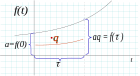
\includegraphics[width=9cm]{allg/funktionen/img/exp/exponentielles_wachstum.png} &
  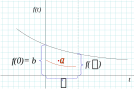
\includegraphics[width=7cm]{allg/funktionen/img/exp/exponentieller_zerfall.png}\\
\end{tabular}

%%\bbwCenterGraphic{10cm}{allg/funktionen/img/exp/exponentieller_zerfall.png}
%%\bbwCenterGraphic{11cm}{allg/funktionen/img/exp/exponentielles_wachstum.png}

Dabei sind
\begin{itemize}
\item $b=f(0)$ der Anfangsbestand zum Zeitpunkt $t$ = 0.
\item $\tau$ ist die typische Zeitspanne zwischen zwei Beobachtungszeitpunkten (zum Beispiel zwischen Wert und dessen Verdopplung). Beispiele:
  \begin{itemize}
  \item Verdoppeln in 3 Stunden: $a=2$ und $\tau = 3\, \text{h}$
    ($\text{h}$ = Stunden)
  \item Verfünf"|fachen einer Viertelstunde (= 15 Minuten): $a=5$ und
    $\tau=\frac{1}{4}\, \text{h}$
  \end{itemize}
  Meist ist die Beobachtungszeit gleichzeitig die Maßeinheit (\zB
  Veränderung pro Stunde). Dann ist unser $\tau=1$ und die Formel
  vereinfacht sich zu $f(t) = b\cdot{}a^t$.
\item $a$ ist der Zunahmefaktor zwischen zwei Beobachtungszeitpunkten (Beispiel $a=2$ bei Verdoppelungsprozessen).
  $a$ berechnet sich durch den Quotienten zwischen zwei
  Beobachtungswerten $a = \frac{f(\tau)}{f(0)} =\frac{m}{b}$.
\item
  Dabei ist $m$ der Messwert zum Zeitpunkt $\tau$.
\item $f(t)=b\cdot{}a^{\frac{t}{\tau}}$ ist der Wert (Anzahl, Fläche,
  Bestand, ...) zum Zeitpunkt
  $t$. 
\end{itemize}

Bemerkung: 
\TNTeop{
$\frac{m}b = \frac{f(\tau)}{f(0)}=\frac{b\cdot{}a^{\frac{\tau}{\tau}}}{b\cdot{}a^{\frac0{\tau}}}
  = \frac{a^1}{a^0} = \frac{a}{1} 
  = a$}%% END TNT
\newpage

\subsection{Referenzaufgabe}\index{Irland!Bevölkerungswachstum}
Irland hatte 1990 3.51 Mio. Einwohner. Im Jahr 2019 waren es bereits 4.93 Mio.

\textbf{Frage 1}: Was prognostizieren Sie für das Jahr 2025, wenn Sie von einem exponentiellen Wachstum ausgehen?

\noTRAINER{\bbwCenterGraphic{12cm}{allg/funktionen/img/exp/IrlandLeer.png}}%%

\TNTeop{
  Skizze:
  \bbwCenterGraphic{12cm}{allg/funktionen/img/exp/IrlandVoll.png}

  $\tau$ = 29 Jahre, Einheit = Jahre ($t$ in Jahren gemessen).
  
  $b=f(0) = 3.51$ [Mio EW] = Startwert (Taschenrechner STO).

  $m=f(\tau) = 4.93$ [Mio EW] = Messwert nach $\tau$ Jahren.

  $a=\frac{m}{b}=\frac{4.93}{3.51} \approx 1.4046$ pro 29 Jahre (Taschenrechner! STO). 

  $$f(t) = b\cdot{}a^\frac{t}{\tau}=b\cdot{}a^\frac{t}{29}$$


  TR Probe $b\cdot{}a^\frac{0}{29} = ? = 3.51$ 

  TR Probe $b\cdot{}a^\frac{29}{29} = ? = 4.93$ 

  Jahr 2025: $t=35$:

    $$f(35) = b\cdot{}a^\frac{35}{29}\approx 5.28899$$

}%% END TNT
\newpage

\subsection*{Aufgaben}

\GESO{\olatLinkArbeitsblatt{Exponentialfunktionen}{https://olat.bms-w.ch/auth/RepositoryEntry/6029794/CourseNode/106029175831971}{Kap. 1.5: Aufg. 18. a) b)}}
\TALS{\olatLinkArbeitsblatt{Exponentialfunktionen}{https://olat.bms-w.ch/auth/RepositoryEntry/6029786/CourseNode/106029175777725}{Kap. 1.5:     Aufg. 18. a) b) }}

\newpage

\textbf{Frage 2}: In wie vielen Jahren hat sich die Bevölkerung verdreifacht?

\TNTeop{
  Gesucht $T_3$ = Verdreifachungszeitpunkt.

  $$f(T_3) = 3\cdot{}f(0)$$

  Funktionsgleichung einsetzen:

  $$b\cdot{}a^\frac{T_3}{\tau} = 3\cdot{} b\cdot{} a^\frac0\tau$$

  Weil $a^{\frac{0}{\tau}} = 1$ folgt:

  $$b\cdot{}a^\frac{T_3}{\tau} = 3\cdot{} b$$

  $$a^\frac{T_3}{\tau} = 3$$

  Def. Logarithmus:

  $$\frac{T_3}{\tau} = \log_a(3)$$

$$T_3 = \tau\cdot{}\log_a(3) = 29\cdot{}\log_a(3) \approx 93.8$$
Die Bevölkerung wird sich voraussichtlich alle 94 Jahren
verdreifachen.

}%% END Trainer
\newpage

\subsection*{Aufgaben}
%%\TALSAadBMTA{221ff}{831 - 839}


\GESO{\olatLinkArbeitsblatt{Exponentialfunktionen}{https://olat.bms-w.ch/auth/RepositoryEntry/6029794/CourseNode/106029175831971}{Kap. 1.5:
    Aufg. 18. c), 19. - 21.}}
\TALS{\olatLinkArbeitsblatt{Exponentialfunktionen}{https://olat.bms-w.ch/auth/RepositoryEntry/6029786/CourseNode/106029175777725}{Kap. 1.5:
    Aufg. 18. c), 19. - 21. }}

\AadBMTA{338}{28. Bakterien}
\AadBMTA{352ff}{2. (Hasenpopulation), 7., 1. (optional)}
\olatLinkGESOKompendium{3.4}{27ff}{32., 34., 38., 40., 44., 45. und 46.}
\GESO{\aufgabenFarbe{Nullserie 2: Aufgabe 8.}}
\GESO{\aufgabenFarbe{Maturaprüfung 2017, Aufg. 12 (Raupen)\\
Maturaprüfung 2018 (Serie 3), Aufg. 11 (Müll)
}}



%% TODO Arbeitsblatt verlinken
%%\GESO{\olatLinkArbeitsblatt{Exponentialfunktionen}{https://olat.bms-w.ch/auth/RepositoryEntry/6029794/CourseNode/106029175831971}{Kap. 1.1: Voraussetzungen}}
%%\TALS{\olatLinkArbeitsblatt{Exponentialfunktionen}{https://olat.bms-w.ch/auth/RepositoryEntry/6029786/CourseNode/106029175777725}{Kap. 1.1: Voraussetzungen}}



\newpage

\subsection{Rate vs. Faktor
  II}\index{Rate}\index{Fatkor}\index{Zunahmefaktor}\index{Zunahmerate}
\totalref{RateZins1}

Den Unterschied von Zinsfuß (= Rate) und Zinsfaktor kennen wir bereits aus der Zinsrechnung.

So entspricht eine Zunahme von 12\% einem\\
Aufzinsungsfaktor von \LoesungsRaumLang{1.12}.

Wenn jedoch eine Beobachtung einer Zunahme von, sagen wir, 70\% innerhalb einer Viertelstunde beobachtet wird, so können wir uns fragen, um wie viel die Zunahme (als Rate oder Faktor) pro Zeiteinheit (hier Stunden) ist.


Füllen Sie dazu folgende Tabelle aus. Dabei bedeuten

\begin{tabular}{lp{14cm}}\hline
  Einheit & Stunden, Minuten, Meter, ... \\\hline
  $\tau$  & In dieser Zeitspanne (Stunden, Meter, ...) wird beobachtet \\\hline
  $p$     & Zunahme\textbf{rate}\index{Zunahmerate}\index{Rate} während $\tau$ Einheiten in \%. Ist $p$ negativ, handelt es sich um eine Abnahme\\\hline
  $a_\tau$ & Zunahme\textbf{faktor}\index{Zunahmefaktor} während $\tau$ Einheiten. Ist $a<1$, handelt es sich um einen Abnahmefaktor\\\hline
  $a_E$ (Formel)   & Zunahme pro Einheit (als Faktor). Aufgeschrieben als Formel\\\hline
  $\approx a_E$ (Zahl)  & Zunahme pro Einheit (als Näherungswert).\\\hline
  $p_E$   & Prozentuale Zunahme pro Zeiteinheit\\\hline
  \end{tabular} 

\leserluft{}
\leserluft{}
%% temporäres Platzhalterchen 
\newcommand{\ph}[1]{\noTRAINER{...........}\TRAINER{#1}}

%%\renewcommand{\arraystretch}{1.7}
$$f(t) = a_\tau^{\frac{t}\tau} = a_E^t$$
%% probably turn off auto-fill-mode in emacs when editing long lines
\begin{bbwFillInTabular}{|l|l|l|l|l|l|l|}\hline
  Einheit & $\tau$            &  $p$         & $a_\tau$         & $a_E$ (Formel)           &  $\approx a_E$    &$p_E$            \\\hline\hline
  h       &  $3$              &  56\%        & $1.56$           & $1.56^\frac13$            &  1.1598           & 11.598\%        \\\hline 
  h       &  $\frac14 = 0.25$ &  70\%        & \ph{1.7}         & \ph{ $1.7^\frac1{0.25}$}  &  \ph{8.3521}      & \ph{735.21\%}   \\\hline 
  h       &  $\frac12$        &  \ph{50\%}   & 1.5              &  $1.5^\frac1{0.5}$        &  2.25             & \ph{125\%}      \\\hline 
  Tage    &  $5$              & 100\%        & \ph{2}           & \ph{$2^\frac1{5}$}        &  \ph{1.1487}      & \ph{14.87}\%    \\\hline 
  Min.    &  $2$              & \ph{-60}\%   & 0.4              & \ph{$0.4^\frac1{2}$}      &  \ph{0.6325}      & \ph{-36.75}\%   \\\hline 
  m       &  $12$             & \ph{4.5}\%   & \ph{1.045}       & $1.045^\frac1{12}$        &  \ph{1.00367}     & \ph{0.3675}\%   \\\hline
  Wochen  & \ph{$2$}          & \ph{$200$}\% & \ph{3}           & $3^\frac12$               & \ph{1.73205}      & \ph{73.205}\%   \\\hline
  Jahr    & \ph{$\frac1{12}$} & \ph{$1$}\%   & \ph{$1.01$}      & $1.01^{\frac1{1/12}}$      &  \ph{$1.127$}     & \ph{$12.7$}\%   \\\hline
\end{bbwFillInTabular} 


\newpage

\subsection{Halbwertszeit, Verdopplungszeit}\index{Halbwertszeit}\index{Verdopplungszeit}

\begin{definition}{Halbwertszeit}{}
Die Zeitspanne, in der sich eine Menge halbiert, nennen wir
\textbf{Halbwertszeit} und bezeichnen diese Zeit mit:

$$T_{1/2}$$
\end{definition}

Die Halbwertszeit wird insbesondere
  beim radioaktiven Zerfall verwendet: nach wie viel tausend Jahren strahlt
  ein Stoff nur noch die Hälfte.


Beispiel: Ein Stoff nimmt innerhalb von sieben Tagen auf 80\% ab. Wie
groß ist seine Halbwertszeit $T_{1/2}$?

\TNTeop{
  Ansatz: $f(t) = b\cdot{}a^{\frac{t}{\tau}}$.

  $80\%$ und $7$ Tage einsetzen:

  $$f(t) = b\cdot{} 0.8^{\frac{t}{7}}$$

  Halber Wert:
  
  $$\frac{b}2= b\cdot{} 0.8^\frac{T_{1/2}}{7}$$
  $$\frac12  = 0.8^\frac{T_{1/2}}{7}$$

  Solver (num-solv): 21.74 (Tage) ...

 ... oder mit der Definition des Logarithmus:
  
  $$\frac{T_{1/2}}7 = \log_{0.8}\left(\frac12\right)$$
  $$T_{1/2} = 7\cdot{} \log_{0.8}\left(\frac12\right) \approx 21.74$$


  Bemerkung: $$f(t) =b\cdot{}0.8^\frac{t}7 \approx b\cdot{}\left(\frac12\right)^\frac{t}{21.74}$$
}%% END TNT
\newpage

\begin{gesetz}{Stoffmenge}{}
  Ist die Halbwertszeit $T_{1/2}$ und die anfängliche Stoffmenge $b$
  bekannt, so kann die Soffmenge zu jedem Zeitpunkt $t$ mit der
  folgenden Funktion $f$ angegeben werden:
  $$f(t) = \LoesungsRaumLen{50mm}{b\cdot{}\left(\frac12\right)^\frac{t}{T_{1/2}}}$$
\end{gesetz}
  
\begin{gesetz}{Halbwertzszeit}{}
  Die Halbwertszeit $T_{1/2}$ berechnet sich wie folgt:
  $$T_{1/2} = \LoesungsRaumLen{70mm}{\log_A\left(\frac12\right) = \tau
  \cdot{} \log_a\left(\frac12\right)}$$
  Dabei ist $A$ der Abnahmefaktor pro Zeiteinheit; $a$ während $\tau$ Zeiteinheiten.
\end{gesetz}


Herleitung:

\TNTeop{
  $$\frac12 \cdot{} f(0) = f(T_{1/2})$$
  $$\frac12 \cdot{} b    = b\cdot{}A^{T_{1/2}}$$
  $$\frac12 = A^{T_{1/2}}$$
  $$\log_A \left(\frac12\right) = T_{1/2}$$
}

\newpage
\GESO{Optional:}

\subsection{Verdopplungszeit}\index{Verdopplungszeit}

Analog gilt das Gesetz zur Verdopplung (s. obiges Beispiel Bevölkerung Irlands):
\begin{gesetz}{Verdopplungszeit}{}
  $$T_2 = \LoesungsRaumLen{40mm}{\log_A(2) = \tau \cdot{} \log_a(2)}$$

  $A$: der Abnahmefaktor pro Zeiteinheit; $a$ während $\tau$ Zeiteinheiten.
  
\end{gesetz}


\subsection*{Aufgaben}

\GESO{\olatLinkArbeitsblatt{Exponentialfunktionen}{https://olat.bms-w.ch/auth/RepositoryEntry/6029794/CourseNode/106029175831971}{Kap. 1.6:
    Halbwertszeit/Verdopplungszeit: Aufg. 22. - 25.}}
\TALS{\olatLinkArbeitsblatt{Exponentialfunktionen}{https://olat.bms-w.ch/auth/RepositoryEntry/6029786/CourseNode/106029175777725}{Kap. 1.6:
    Halbwertszeit/Verdopplungszeit: Aufg. 22. - 25.}}

\AadBMTA{352ff}{3. (Taucherin), 4. [Glasfaser ohne Teilaufgabe
    Eindringtiefe 4. b)] und 5. b) (radioaktiver Zerfall)}

\olatLinkGESOKompendium{3.4}{28ff}{42., 43. und 47.}

\GESO{\aufgabenFarbe{
    Maturaprüfung 2020, Aufg 11 (Käfer)\\
    Maturaprüfung 2018 (Serie 4), Aufg 10 (Cäsium 137)\\
    Maturaprüfung 2018 (Serie 2), Aufg 11 (Plutonium)\\
    Maturaprüfung 2018 (Serie 1), Aufg 11 (radioaktive Substanz)\\
    Maturaprüfung 2016, Aufg. 9 (Jod-131)
}}

\olatLinkGESOKompendium{3.4}{27ff}{32. bis 47.}

\newpage
\newpage
\section{Sättigungsprozesse, beschränktes Wachstum}
\sectuntertitel{Ich kann nicht mehr...}

\subsection*{Lernziele}
\begin{itemize}
	\item Grundformel eines Sättigungsfunktion
  \item Funktionsterm bei gegebenen Randbedingungen 
\end{itemize}

Bei beschränktem Wachstum ist die Änderungsrate typischerweise
proportional zur
sog. \textbf{Sättigungsdifferenz}\index{Sättigungsdifferenz}\index{Differenz!zur
  Sättigung}
(auch Sättigungs\textbf{manko}\index{Sättigungsmanko}\index{Manko!der
  Sättigung} oder Sättigungsdefizit\index{Sättigungsdefizit}).
  So bezeichnet man die \textbf{Differenz} zwischen dem
  aktuellen Wert und der Sättigungsgreze.

Mit anderen Worten: Je weiter weg der aktuelle Wert vom Grenzwert ist, umso rascher ist die Zunahme (bzw. die Abnahme bei beschränktem Zerfall).

\newpage


\subsection{Beispiele von Sättigungsprozessen}
Überlegen Sie sich Beispiele von Prozessen, bei welchen eine bestimmte Schwelle nicht überschreiten bzw. unterschritten werden kann:
\begin{itemize}
	\item \Lueckentext{Laden einer Batterie (je weniger geladen, um so schneller lädt sie)}
	\item \Lueckentext{Druck ablassen aus einem Pneu (je mehr Druck, umso schneller entweicht er)}
	\item \Lueckentext{Abkühlen eines Getränks bis zur Zimmertemperatur}
	\item \Lueckentext{Aufwärmen eines Getränks auf 40 Grad Celsius}
	\item \Lueckentext{Wirkstoffniveau bei Einnahme von Medikamenten.}
	\item \Lueckentext{Populationszunahme bei beschränkten Ressourcen (Futter, Platz, ...)}
        \item \Lueckentext{Lernkurve}
        \item \Lueckentext{\dotfill}
\end{itemize}
\newpage


\subsection{Begrenzter Zerfall}\index{Begrenzter Zerfall}\index{Zerfall!begrenzter}

\subsubsection{Einstiegsbeispiel Tee}\index{Tee!Abkühlungsprozess}\index{Abkühlungsprozess}

Tee wird von 75 Grad Celsius auf Zimmertemperatur (20 Grad)
abgekühlt. Nach drei Minuten messen wir 61 Grad.


a) Skizzieren Sie die «Zerfallskurve», welche die Temperatur des Tees
angibt.

b) Geben Sie die Funktionsgleichung $f(t)$ an, welche den Prozess
beschreibt.

c) Wann ist die Temperatur auf angenehme 37 Grad gesunken?


\TNTeop{1. Idee mit gleicher Formel klappt nicht, denn der
  Standard-Exponentielle Zerfall geht nach Null!

  Skizze mit 75 Grad, 20 Grad (Sättigung) und 51 Grad.

2. Idee: verschiebe die Skala um 20 Einheiten nach unten. Nun
funktioniert es: $g(t) = 55\cdot{}\left(\frac{41}{55}\right)^{\frac{t}{3}}$

3. Verschiebe wieder zurück: ACHTUNG: Das $b$ ist nun jedoch die
Sättigungs\textbf{differenz} zum Zeitpunkt $t_0=0$ und \textbf{nicht} mehr der Startwert! 

$$f(t) = 20 + g(t) = 20 + 55\cdot{}\left(\frac{41}{55}\right)^{\frac{t}{3}}$$

4. Berechnung: Wann sind 37 Grad erreicht? Einsetzen
in die Funktionsgleichung:

$$37\degre = y=f(t) = 20 + 55\cdot{}\left(\frac{41}{55}\right)^{\frac{t}{3}}$$

$$17=55\cdot\left(\frac{41}{55}\right)^\frac{t}{3}$$

$$\frac{17}{55}=\left(\frac{41}{55}\right)^\frac{t}{3}$$

$$\frac{t}3 = \log_{\left(\frac{41}{55}\right)}\left(\frac{17}{55}\right)$$


$$t=3\cdot{}\log_{\left(\frac{41}{55}\right)}\left(\frac{17}{55}\right)\approx
11.99 \textrm{ min.}$$

}%% END TNT

\newpage

\subsubsection{Allgemeine Form des beschränkten Zerfalls}
\begin{center}
\raisebox{-1cm}{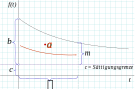
\includegraphics[width=13cm]{allg/funktionen/img/saettigung/saettigungskurveDown.png}}
\end{center}

Die Grundform eines begrenzten Zerfalls ist ein normaler
exponentieller Zerfall ($y=a^{t}$, $0<a<1$), der in $y$-Richtung um eine Sättigungsgrenze $c$ verschoben ist:

\begin{definition}{beschränkter Zerfall}{}
$$f(t) = c + b\cdot{}a^{\frac{t}{\tau}}$$
\end{definition}

Dabei ist:
\begin{itemize}
  \item $c+b = f(0) = y$-Achsenabschnitt = Startwert
	\item $c$: Die Sättigungsgrenze\index{Sättigungsgrenze} (Sättigungswert). Dies ist die Annäherungskonstante oder der \textbf{Asymtote}nwert\index{Asymptote}: Tiefer kann die Funktion nicht fallen.

	\item $m$:
    Sättigungs\textbf{differenz}\index{Sättigungsdifferenz}\index{Differenz!zur
      Sättigung}. Wie viel fehlt, bis zur
    Sättigungsgrenze: $m = f(t) - c$. Die Sättigungs\textbf{differenz} nimmt exponentiell ab.
	\item $b$: Die \textbf{Abweichung} zu $c$ zum Zeitpunkt $t=0$. Der
    Anfangswert ist somit $f(0) = c + b$; mit anderen Worten: $b$ ist das
    \textbf{Sättigungsdifferenz} zum Zeitpunkt $t_0 = 0$.

    \item $a=\frac{m}{b}=\frac{f(\tau)-c}{f(0)-c}$: Der Faktor der Veränderung der
      Sättigung\textbf{differenz}.
\end{itemize}

\subsection*{Aufgaben}
\GESOAadBMTA{359}{35. (Kuchen) und 36. (Ovomaltine)}
\olatLinkGESOKompendium{3.4.2}{33}{48. (Achtung: Das
  Kompendium verwendet andere Buchstaben: Das dortige $a$ ist unser $b$.)}

\GESO{\olatLinkArbeitsblatt{Exponentialfunktionen}{https://olat.bbw.ch/auth/RepositoryEntry/572162163/CourseNode/106029175831971}{Kap. 3.1:
    Sättigung: Begrenzter Zerfall}}
\TALS{\olatLinkArbeitsblatt{Exponentialfunktionen}{https://olat.bbw.ch/auth/RepositoryEntry/572162090/CourseNode/106029175777725}{Kap. 3.:
    Sättigung: Begrenzter Zerfall}}
\newpage


\subsection{Sättigung (begrenztes Wachstum)}\index{Sättigung}\index{begrenztes Wachstum}\index{Wachstum!begrenztes}
\subsubsection{Einstiegsbeispiel 1: Eistee wärmen}
Das Aufwärmen von Eistee von $5\degre$ Kühlschranktemperatur auf $20\degre$ Zimmertemperatur ist ein klassisches «Begrenztes Wachstum» (mit gespiegelter Exponentialfunktion).

\TNT{5.2}{Skizze}

\subsubsection{Einstiegsbeispiel 2: Batterie laden}
\begin{center}
\raisebox{-1cm}{
\includegraphics[width=8cm]{allg/funktionen/img/saettigung/batterien.png}}
\end{center}

Eine 9V-Batterie ist etwas mehr als zur Hälfte entladen und enthält nun eine
Restspannung von 4V.

Wenn wir 9V an die Batterie anlegen, so wird die Batterie geladen.

Die Batterie lädt sich umso rascher, je \textit{leerer} sie ist.

Die Batterie lädt sich umso langsamer, je \textit{voller} sie ist.


\newpage

\subsubsection{Allgemeine Form von Sättigungsprozessen}

\begin{center}
\raisebox{-1cm}{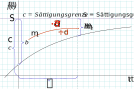
\includegraphics[width=13cm]{allg/funktionen/img/saettigung/saettigungskurve.png}}
\end{center}

Die Grundform des begrenzten Wachstums ist ein exponentieller Zerfall\totalref{zerfallsfunktion},
der an der $x$-Achse gespiegelt und in $y$-Richtung
verschoben ist:

\begin{definition}{Sättigung}{}
$$f(t) =c - b\cdot{} a^{\frac{t}{\tau}}$$
\end{definition}

Die Variable haben die folgenden Bedeutungen:

\begin{itemize}
	\item $c$: Sättigungsgrenze. Dies ist die Annäherungskonstante oder der Asymtotenwert. Höher kann die Funktion nicht steigen.

	\item $m$ ist die
    Sättigungsdifferenz\index{Sättigungsdifferenz}\index{Differenz!zur
    Sättigung}. Wie viel fehlt, bis zur
    Sättigungsgrenze: $m = c - f(t)$. Auch hier nimmt die Sättigungs\textbf{differenz} exponentiell ab.
	\item $b$: Die Abweichung des Funktionsgraphen zu $S$ zum Zeitpunkt $t=0$. Der
    Anfangswert ist somit $f(0) = c - b$.
\item $a=\frac{m}{b}=\frac{c-f(\tau)}{c-f(0)}$ Faktor der Veränderung
  der Sättigungs\textbf{differenz}.
\end{itemize}


\subsubsection{Bemerkungen}
\begin{bemerkung}{}{}
  Für die Sättigungsdifferenz gilt:

\TNT{4}{$$m = m(t) = c - f(t) = c - \left(c-b\cdot{}a^{\frac{t}{\tau}}\right) = + b\cdot{}a^{\frac{t}{\tau}}$$

und somit:

$$m_0 = m(0) = b\cdot{}a^0 = b$$}%% END TNT
\end{bemerkung}

\TRAINER{ Bemerkung (Trainer/mündlich):
  
Das $a$ kann aus zwei \textbf{beliebigen} Sättigungsdifferenz-Werten berechnet werden (die um die
Zeitdifferenz $\tau$ auseinander liegen):
$$\frac{m_2}{m_1} = \frac{b\cdot{}a^{\frac{t_2}{\tau}}}{b\cdot{}
  a^{\frac{t_1}{\tau}}} = a^{\frac{t_2}{\tau}} : a^{\frac{t_1}{\tau}} =
a^{\frac{t_2-t_1}{\tau}} = a^{\frac{\tau}{\tau}} = a$$%% 
}%% END Trainer


\begin{bemerkung}{}{}
Meistens ist $m_0$ zum Zeitpunkt $t=0$ bekannt und somit ist $b=m_0$. Es reicht, die Messung zum Zeitpunkt $t_0$ und zu einem weiteren Zeitpunkt durchzuführen. Wenn zusätzlich die Sättigungsgrenze $c$ bekannt ist, kann die Funktion $f$ komplett bestimmt werden.
\end{bemerkung} 

\newpage

\subsection{Referenzaufgaben}

\subsubsection{Berechnung am Batterie-Beispiel}\index{Batterie}
Eine Batterie weist zum Zeitpunkt $t_0$ vier Volt auf. Nach sechs Stunden am Ladegerät zeigt die Messung sieben Volt. Wir wissen, dass die Sättigungsgrenze (Ladespannung) bei neun Volt liegt.

Zeichnen Sie die gegebenen Größen in ein Koordinatensystem ein und markieren Sie bei neun Volt eine horizontale Beschränkungslinie (\zB 1V = 1 Häus'chen in $y$-Richtung; 1h = 1 Häus'chen in $x$-Richtung).

\noTRAINER{\mmPapier{8.8}}
\TRAINER{\bbwCenterGraphic{15cm}{allg/funktionen/img/saettigung/batterieFct.png}}

\textbf{Frage 1}: Wie lautet die Formel $f(t) = ...$ der Sättigungskurve?

\noTRAINER{$c = ..........................$}
\TRAINER{$c = \textrm{ Sättigungsgrenze } = 9 [\textrm{V}]$}

\noTRAINER{$b = ..........................$}
\TRAINER{$b = m_0 = c-f(0) = 9 - 4 = 5$}

\noTRAINER{$m =  ..........................$}
\TRAINER{$m = m_1 = c-f(\tau) = 9 - 7 = 2$}

\noTRAINER{$a = .........................$}
\TRAINER{$a=\frac{m}{b} = \frac{m_1}{m_0} = \frac{2}{5} = 0.4$}

\noTRAINER{$\tau = .........................$}
\TRAINER{$\tau = 6$ ($e_x$ = eine Stunde)}


\noTRAINER{$f(t) = c - b\cdot{}a^{\frac{t}{\tau}} = ..... - .....\cdot{}(.....)^{\frac{-t}{.....}}$}
\TRAINER{$f(t) = c - b\cdot{}a^{\frac{t}{\tau}} = 9 - 5\cdot{}(\frac{2}{5})^{\frac{t}{6}}$}

\TRAINER{Die Kontrollen für $t=0$ und $t=6$ sind mit dem Stehenlassen von $a$ als Bruch nun sehr einfach.}
\newpage

\textbf{Frage 2}: Wann wird die Batterie zu 99\% geladen sein?

\TNTeop{99\% von 9V = 8.91 V

  Somit ist $t$ gesucht mit $f(t) = 9 - 5\cdot{}\left(\frac25\right)^{\frac{t}{6}} = 8.91$

  (beidseitig -9 und Vorzeichen drehen und dann durch 5 teilen, so folgt...)

  $$(0.4)^{\frac{t}{6}} = (9-8.91) : 5 = 0.09 : 5 = 0.018$$

  Definition Logarithmus:

  $$\frac{t}6 = \log_{0.4}(0.018) \approx 26.3 $$

  Nach ca. 26 - 27 Stunden ist die Batterie zu 99\% geladen.
}
\newpage

\subsubsection{Referenzaufgabe Sättigung: Pneu}\index{Reifen}\index{Pneu}

Ein Reifen (Pneu) ist anfänglich ganz leer und enthält «nur» 1 atm, nämlich den
Druck der Umgebung. (1 atm = atmosphärischer Druck = technische Atmosphäre) 

Der Reifen wird aufgepumpt mit einer Druckpumpe, die maximal 2 atm
leisten
kann. Mit 2 atm ist hier gemeint: 2 at mehr als der
Umgebungsdruck. Somit könnte der Pneu bis auf maximal 3 atm aufgepumpt
werden (= Sättigungsgrenze).

Um den Reifen optimal zu füllen, wird er auf 2 atm aufgepumpt (1 atm
über dem Umgebungsluftdruck).

Die Pumpe schafft in den ersten 10 Sekunden den Druck von 1 atm auf 1.2
atm (= 0.2 atm über Normaldruck) aufzupumpen.

Nach wie vielen Sekunden muss gestoppt werden, damit der Reifen
optimal gepumpt ist?

\TNTeop{Die Sättigungsdifferenz schwindet von $m_1=3-1=2$ bis $m_2=3-1.2=1.8$
innerhalb der ersten $10s = \tau$. Die Sättigungsgrenze liegt bei
$S=3$. Unsere (Exponential)basis $a$ ist somit $1.8 / 2$, was uns
liefert:
$$f(t) = 3 - 2\cdot{}\left(\frac{1.8}{2}\right)^\frac{t}{10}$$
Somit ist das Optimum bei $2 = 3-
2\cdot{}\left(\frac{1.8}{2}\right)^\frac{t}{10}$ erreicht, also bei
etwa 65.8 Sekunden.
}
\newpage

\GESO{\subsection*{Aufgaben}}
\GESOAadBMTA{358}{34. (Eistee)}
\olatLinkGESOKompendium{3.4.2}{32ff}{49. - 51. (Bem.: Das
  Kompendium gibt die Funktionsterme bereits an und verwendet als
  Basis i.\,d.\,R. die Eulersche Konstante $e\approx{} 2.71828$)}

\GESO{\olatLinkArbeitsblatt{Exponentialfunktionen}{https://olat.bbw.ch/auth/RepositoryEntry/572162163/CourseNode/106029175831971}{Kap. 3.1:
    Begrenztes Wachstum}}%% END GESO
\TALS{\olatLinkArbeitsblatt{Exponentialfunktionen}{https://olat.bbw.ch/auth/RepositoryEntry/572162090/CourseNode/106029175777725}{Kap. 3.1:
    Begrenztes Wachstum}}%% END TALS

\newpage

\subsection{Zusammenfassung der Prozesse}
\vspace{8mm}
\begin{center}\textbf{Wachstum und Zerfall}\end{center}

\TNT{8.8}{\bbwCenterGraphic{18cm}{allg/funktionen/img/zusammenfassung_exp/wachstum_zerfall.png}

  bzw.
  $$f(t) = G_0 \cdot{} \e^{qt}; q=  \frac{\ln(a)}\tau  \,\,\,\,\,\,\,\,\, f(t) = G_0 \cdot{} \e^{-qt}; q  = \frac{-\ln(a)}\tau$$
}%% END TNT

\vspace{8mm}
\begin{center}\textbf{Sättigung}\end{center}

\TNTeop{\bbwCenterGraphic{18cm}{allg/funktionen/img/zusammenfassung_exp/saettigung.png}

    bzw.
     $$f(t) = S + (G_0-S) \cdot{} \e^{q\cdot{}t}; q=    \frac{\ln(a)}\tau     \,\,\,\,\,\,\,\,\, f(t) = S + (S - G_0) \cdot{} \e^{-q\cdot{}t}; q  = \frac{-\ln(a)}\tau$$

Hier ist Platz für das Video/die Videos zur den getanzten
Funktionen (S. OLAT/Wiki).
}%% END TNTeop

\newpage

\TALS{
  \subsection*{Aufgaben}
  \olatLinkTALSStrukturaufgabenSPF{Basiskenntnisse Funktionen Teil
    1}{5}{4., 5., 8. und 9.}
  \olatLinkTALSStrukturaufgabenSPF{Basiskenntnisse Funktionen Teil
    2}{14}{45., 47. und 49.}
}%% END TALS
\newpage


%%%%%%%%%%%%%%%%%%%%
% Arithmetik und Algebra II
%%%%%%%%%%%%%%%55
%% Funktionen II GESO Metapackage
\part{Funktionen II}\index{Funktionen!II|textbf}
\renewcommand{\bbwPartID}{FCT2}
\section{Potenzfunktionen}\index{Funktion!Potenzfunktionen}\index{Potenzfunktionen}
\sectuntertitel{Funktionen hoch drei!}

\subsection*{Lernziele}

\begin{itemize}
\item Definition Ganzzahlige Potenzfunktion
\item Graphische Darstellung
\end{itemize}
\newpage


\subsection{Einstieg}

%%%%%%%%%%%%%%%%%%%%%%%%%%%%%%%%%%%%%%%%%%%%%%%%%%%%%%%%%%%%%%%%%
\subsubsection{Beispiel: Rationale Funktion\GESO{ (optional)}}

Betrachten wir einmal die Funktion $f: y = 0.1x^3 + x^2 + 2x + 3 - x^{-1}$ \zB mit Geogebra (\texttt{www.geogebra.org}).

\bbwGraph{-10}{4}{-7}{8}{%
  \bbwFunc{0.1*\x*\x*\x + \x*\x + 2*\x + 3 -1/\x}{-8.5:-0.2}
  \bbwFunc{0.1*\x*\x*\x + \x*\x + 2*\x + 3 -1/\x}{0.1:1.5}
}%%


Polynomfunktionen und rationale Funktionen sind «\textit{weiche}» Funktionen, die jedoch \textbf{Asymptoten}\index{Asymptote} (hier bei $x=0$) aufweisen können.
Ebenso sind die Extremwerte (lokale Maxima und Minima)\TALS{ wie auch die Wendepunkte} charakteristische Stellen und oft Gegenstand der Untersuchung.
Wir beschränken uns \TALS{vorerst }auf Funktionen der Art $f: y=a\cdot{}x^z$
mit $z \in \mathbb{Z}\backslash\{0\}$\TRAINER{ $z=0$ ist eine
  Proportionalität und somit hier unspannend}.

\newpage



\subsubsection{\GESO{Beispiel}\TALS{Repetition}: Reinquadratische Funktion}\index{quadratische Funktion}\index{Funktion!quadratische}

Zeichnen Sie den Graphen der Funktion $f: y= \frac16 x^2$:

\bbwGraph{-7}{7}{-1}{6.5}{%%
  \TRAINER{
    \bbwFunc{\x*\x/6}{-6:6}
  }
}%%

\begin{definition}{Reinquadratische Funktion}{}
Die Funktion

$f: y = a\cdot{}x^2$

heißt \textbf{Parabel zweiter Ordnung} oder rein-quadratische Funktion.
\end{definition}


\TALS{
\begin{bemerkung}{}{}
Eine allgemeine quadratische Funktion besitzt auch noch einen linearen ($bx$) und einen konstanten ($c$) Anteil. Die allgemeine quadratische Funktion hat die Form

$$f: y= ax^2 + bx + c$$
\end{bemerkung}
}%% END TALS

\TALS{Beispiele zu allgemeinen quadratischen Funktionen finden sie im
  Buch \cite{marthaler21alg} ab Seite 260 insb. im Bild zu Aufg. 4 auf
  Seite 273.}%% END TALS

\newpage

\subsection{Parabel}\index{Parabel}

Zeichnen Sie $y = \frac{1}{16}x^4$ im Bereich $[-3; 3]$ indem Sie für jeden 0.5-er $x$-Wert das zugehörige $y$ berechnen:

\bbwGraph{-4}{4}{-1}{6.5}{%%
  \TRAINER{\bbwFunc{\x*\x*\x*\x/16}{-3:3}}
}%%


\begin{definition}{Parabel}{definition_parabel}
  Ist $n\in \mathbb{N}_{\ge 2}$, so wird der Graph der Potenzfunktion
  $$x\mapsto a\cdot{}x^n$$
  \textbf{Parabel} $n$-ter Ordnung genannt.
\end{definition}

\TALS{%%
\begin{bemerkung}{Potenzfunktion}{definition_potenzfunktion}
  Eine Funktion der Art
$$f: y=a\cdot{}x^r$$
  mit $r \in \mathbb{R}\backslash\{0\}$ heißt \textbf{Potenzfunktion}.
\end{bemerkung}

\begin{bemerkung}{Polynomfunktionen}{}
  Funktionen, deren Funktionsterm ein Polynom bilden werden
  \textbf{Polynomfunktionen} genannt:
  $$f: y=a_n\cdot{}x^n + a_{n-1}\cdot{}x^{n-1} + a_{n-2}\cdot{}x^{n-2} + ... + a_2\cdot{}x^2 + a_1 \cdot{} x + a_0 $$
\end{bemerkung}
%
}%% END TALS


\newpage
\subsection*{Aufgaben}
\aufgabenFarbe{Zeichnen Sie die Parabeln $$y=f(x) = x^n$$ für $n = 2$,
  $n=3$, $n=4$, $n=5$ und $n=6$ mit \texttt{geogebra.org}.
\\
Was fällt auf?}
%%\GESOAadBMTA{303ff}{1. (nur $n=3$ und $n=5$), 2. (nur $n=4$ und $n=6$)}

\TNTeop{}

\newpage

\subsubsection{Anwendung (optional)}
Boltzmannsches T-hoch-vier-Gesetz\index{Boltzmann!$T^4$-Gesetz}

\leserluft{}

Die Funktion $P(T) = \sigma\cdot\varepsilon\cdot
  A\cdot{}T^4$ beschreibt, welche Strahlungsleistung $P$ ein Körper der
  Oberfläche $A$ (in $ \text{m}^2$) bei Temperatur $T$ (in Kelvin) aussendet.

  $\sigma$ = Bolzmann Konstante = $5.6\cdot{}10^{-8}$
  
  $\varepsilon$ = Emissionswert

  \small{\texttt{(eg. https://ennologic.com/wp-content/uploads/2018/07/Ultimate-Emissivity-Table.pdf)}}

  \leserluft{}
  
  Rechenbeispiel:

\TNTeop{$T$ = 20 Grad Zimmertemperatur in Kelvin: 293.15;
  Brick (Haus) hat Emissionswert ca. 0.75; Haus Oberfläche $500 \text{m}^2$

  $$P(293.15) \approx 5.6\cdot{}10^{-8} \cdot{} 0.75 \cdot{} 500
  \cdot{} 293.15^4 \approx 155 \text{kW} $$
  Natürlich strahlt eine 20-grädige Umgebungstemperatur gleich viel
  wieder zurück, sodass keine 'Heizkosten' entstehen.

  Heizen wir das Haus nun zwei Grad wärmer, so erhalten wir:
  $$P(295.15) \approx 5.6\cdot{}10^{-8} \cdot{} 0.75 \cdot{} 500
  \cdot{} 295.15^4 \approx 159.4 \text{kW} $$

  Dies entspricht einer Differenz von 4.28 kW für nur zwei Grad wärmer
  im Haus!
  

}%% END TNT
\newpage

Zeichnen Sie des weiteren die Funktion $y = \frac{1}{9}x^3$:

\bbwGraph{-4}{4}{-5}{5}{%%
  \TRAINER{\bbwFunc{\x*\x*\x/9}{-3.5:3.5}}
}%%

\subsubsection{Symmetrien}\index{Symmetrien!von Parabeln}\index{Parabel!Symmetrie}
Was fällt für gerade und ungerade Exponenten auf? Gibt es Spiegelachsen
oder Spiegelpunkte?

\renewcommand{\mmPapier}[1]{\mmPapierZwei{#1}{16.4}}
\begin{tabular}{c|p{8cm}}
  $x^2$ & \vspace{0.1mm}\TNT{0.8}{An der $y$-Achse}\\\hline
  $x^3$ & \vspace{0.1mm}\TNT{0.8}{Am Ursprung $O(0|0)$}\\\hline
  $x^4$ & \vspace{0.1mm}\TNT{0.8}{wie $x^2$}\\\hline
  $x^5$ & \vspace{0.1mm}\TNT{0.8}{wie $x^3$}\\\hline
\end{tabular}
\renewcommand{\mmPapier}[1]{\mmPapierZwei{#1}{17.6}}


\GESO{Eine Zusammenfassung der wichtigsten Eigenschaften von
  Potenzfunktionen finden Sie im Buch \cite{marthaler21alg} Seite 296 oben.}
\newpage

\subsubsection{Referenzaufgabe}

Bestimmen Sie $a$ und $k$ so, dass der Graph von $y = a \cdot{} x^k$
durch die Punkte $P=\left(3 \middle| 1458\right)$ und
$Q=\left(-4\middle|8192\right)$ verläuft.

\TNT{15.2}{ Punkte einsetzen in die Funktionsgleichung:
  \gleichungZZ{1458}{a\cdot{}3^k}{8192}{a\cdot{}(-4)^k}
  Aus der oberen Gleichung das $a$ ermitteln ($a=\frac{1458}{3^k}$)
  (I) und in die zweite
  Gleichung einsetzen: $$8192 = \frac{1458}{3^k} \cdot{} (-4) ^k$$
  Exponent $k$ separieren:
  $$\frac{8192}{1458} = \left(\frac{-4}3\right)^k$$
  Problem: Logarithmen mit negativen Basen (hier $\frac{-4}3$)
  funktionieren nicht!
  
  Weil nun $k$ gerade sein muss, folgt dass $\left(\frac{-4}3\right)^k
  = \left(\frac43\right)^k$. Daraus ergibt sich
  $$\frac{8192}{1458} = \left(\frac{4}3\right)^k \Longrightarrow k =
  \log_{\frac43}\left(\frac{8192}{1458}\right) = 6$$
  Dieses $k$ nun in die Gleichung (I) einsetzen; dies
  liefert
  $$a=\frac{1458}{3^k} = 2.$$
}%% end TRAINER


\subsection*{Aufgaben}
\AadBMTA{305ff}{11. a) b) c), 13. a) c), (optional 17.,)  18.}
%%\TALSAadBMTA{197}{735. (6) (7) und (9) jeweils mit geogebra, 736. a) d),
%%  737. a) c), 739.}
\newpage


\subsection{Translationen}\index{Manipulation!Funktionen}\index{Funktions-Manipulation}\index{Translation!Funktion}
\sectuntertitel{Manipulation an Funktionsgraphen}
(Verschiebung\index{Verschiebung}, Spiegelung\index{Spiegelung},
Streckung\index{Streckung})

\TadBMTA{217}{13.3}
%%\TALSTadBFWA{163}{3}
Betrachten Sie die Funktionen

$$f(x) = a\cdot{}\left(\frac{x\TALS{-d}}b\right)^5\TALS{+c}$$
und
$$g(x) = a\cdot{}\left(\frac{x\TALS{-d}}b\right)^4\TALS{+c}$$

mit Geogebra (\texttt{geogebra.org})
und beschreiben Sie die Effekte der Parameter

$a$: \TRAINER{Streckung in $y$-Richtung. $a$ negativ: Spiegelung an der
$x$-Achse.}

\noTRAINER{\mmPapier{2.4}}

$b$: \TRAINER{Streckung entlang der $x$-Achse. $b$ negativ: Spiegelung
  an der $y$-Achse.}

\noTRAINER{\mmPapier{2.4}}

\TALS{%% nur TALS haben Verschiebungen
  $c$: \TRAINER{Verschiebung entlang der $y$-Achse}

\mmPapier{2.4}
}%% end TALS

\TALS{
$d$: \TRAINER{Verschiebung entlang der $x$-Achse (Verschiebung nach
  rechts verlangt ein negatives $d$.)}

\noTRAINER{  \mmPapier{2.4}}
}%% END TALS

\newpage

\subsubsection{Zusammenfassung der Translationen}


Wir betrachten die verschiedenen geometrischen
Funktions-«Manipulationen» (Abbildungen) am Beispiel {\color{red}$y =f(x) = \frac18 x^3$}.


\newcommand{\graphTranslationMultiColumn}[5]{%
  \multicolumn{3}{|l|}{#1}\\%%
\hline%%
\graphTranslationMultiColumnZ{#2}{#3}{#4}{#5}
}%% end new command \graphTranslationMultiColumn

\newcommand{\graphTranslationMultiColumnZ}[4]{%
\multirow{5}{6cm}{#1} &  & \multirow{2}{*}{\begin{minipage}{.3\textwidth}\raisebox{-8cm}{\includegraphics[width=\linewidth,height=60mm]{allg/funktionen/img/translation/#4}}\end{minipage}}\\[55mm]%%
&\fbox{#2}&\\%%
&&\\%%
&{\color{red}\fbox{#3}}&\\%%
&&\\%%
\hline%%
}%% end new command \graphTranslationMultiColumnZ

\TALS{%% Nur TALS haben Verschiebungen
\begin{tabular}{|p{7cm}|c|c|}%%
\hline%%
\graphTranslationMultiColumn{Verschiebung in $y$-Richtung...}{... um \textbf{zwei} Einheiten nach \textbf{oben}:}{$g(x)=f(x)\textbf{+2}$}{$g(x)=\frac18x^3\textbf{+2}$}{typ1.png}
\graphTranslationMultiColumnZ{... um \textbf{eine} Einheiten nach \textbf{unten}:}{$g(x)=f(x)\textbf{-1}$}{$g(x)=\frac18x^3\textbf{-1}$}{typ2.png}
\end{tabular}%%
}%% end TALS

\begin{tabular}{|p{7cm}|c|c|}%%
\hline%%
\graphTranslationMultiColumn{Spiegelung...}{... an der $x$-Achse:}{$g(x)=-f(x)$}{$g(x)=-\frac18x^3$}{typ3.png}
\graphTranslationMultiColumnZ{... an der $y$-Achse:}{$g(x)=f(-x)$}{$g(x)=\frac18(-x)^3$}{typ4.png}
\end{tabular}%%

\begin{tabular}{|p{7cm}|c|c|}%%
\hline%%
\graphTranslationMultiColumn{Streckung...}{... in $y$-Richtung (von der $x$-Achse aus) um Faktor \textbf{zwei}:}{$g(x)=\textbf{2}\cdot{}f(x)$}{$g(x)=\textbf{2}\cdot{}\frac18x^3$}{typ5.png}
\graphTranslationMultiColumnZ{... in $x$-Richtung (von der $y$-Achse aus) um Faktor \textbf{zwei}:}{$g(x)=f(\frac{1}{\textbf{2}}\cdot{}x)$}{$g(x)=\frac18(\frac{1}{\textbf{2}}\cdot{}x)^3$}{typ6.png}
\end{tabular}%%

\TALS{%% Nur TALS verschieben in x-Richtung
\begin{tabular}{|p{7cm}|c|c|}%%
\hline%%
\graphTranslationMultiColumn{Verschiebung in $x$-Richtung\footnote{Kein prüfungsrelevantes Thema.}...}{... um \textbf{zwei} Einheiten nach \textbf{links}:}{$g(x)=f(x\textbf{+2})$}{$g(x)=\frac18(x\textbf{+2})^3$}{typ7.png}
\graphTranslationMultiColumnZ{... um \textbf{zwei} Einheiten nach \textbf{rechts}:}{$g(x)=f(x\textbf{-2})$}{$g(x)=\frac18(x\textbf{-2})^3$}{typ8.png}
\end{tabular}%%
}%% END TALS
\newpage

\subsection*{Aufgaben}
\GESO{
Skizzieren Sie $-\frac{1}{2}x^3 - 1$ im Bereich $x$ = -2 bis $x$ = +2.

\bbwGraph{-4}{4}{-5}{3}{%%
  \TRAINER{%
    \bbwFunc{-0.5*\x*\x*\x-1}{-2:2}%
  }%%
}%

Vergleichen Sie die neue Funktion mit der Parabel $y=x^3$.

\TNT{5.2}{Die neue Funktion ist an der $y$-Achse gespiegelt, ist um
  50\% gestaucht ($y$-Richtung) und ist um eine Einheit nach unten
  ($x$-Richtung) verschoben worden.}
}%% END GESO

\AadBMTA{304ff}{5. a) c) d) e), 9. a) d) e)}

 
\TALS{
  \aufgabenFarbe{Zeichnen Sie mit \texttt{geogebra.org} die Funktion
    $f(x) = \frac1{10}(x^3 - 3x^2 + 3)$
    \\
    Definieren Sie anschließend die Funktion $$g(x) = a\cdot{}f((x+s)\cdot{}b)+r.$$
\\
    Entscheiden Sie, welche Veränderungen die Parameter $a$, $b$, $r$
    und $s$ bewirken.\\
    Starten Sie mit $a=1$, $b=1$, $r=0$ und $s=0$.
  }%% END Aufgabenfarbe
  \TNT{4}{
    $r$: Verschiebung nach oben\\
    $s$: Verschiebung nach links\\
    $a$: Streckung in $y$-Richtung\\
    $b$: Stauchung in $x$-Richtung
  }%% END TNT
}%% END TALS



%%  OLAT Arbeitsblatt
\GESO{\olatLinkArbeitsblatt{Positive Potenzfunktionen zuordnen}{https://olat.bbw.ch/auth/RepositoryEntry/572162163/CourseNode/104752086007823}{(alle Beispiele)}}%% END olatLinkArbeitsblatt
\TALS{\olatLinkArbeitsblatt{Positive Potenzfunktionen zuordnen}{https://olat.bbw.ch/auth/RepositoryEntry/572162090/CourseNode/105597875231723}{(alle Beispiele)}}%% END olatLinkArbeitsblatt


\olatLinkTALSStrukturaufgabenSPF{Teil 2}{15ff}{48. und 51.}
%%\TALS{\aufgabenFarbe{Strukturaufgaben SPF Teil 2: Taschenrechner: S. 15ff:  Aufg. 48. und 51.}%% END Aufgabenfarbe
%%}%% END TALS

%%\TALSAadBMTA{197 ff.}{739., 743. c), 745. c), 738.*}

\olatLinkGESOKompendium{3.3.1.}{26}{28., 29.}
\newpage



%%%%%%%%%%%%%%%%%%%%%%%%%%%%%%%%%%%%%%%%%%%%%%%%%%%%%%%%%%%%%%%%%%%%%%%%%%%%%%%%%%%
\subsection{Hyperbel}\index{Hyperbel (negative Exponenten)}

(«Hyperbel» Griechisch = «über das Ziel hinaus werfen»)


Zur Erinnerung:
\begin{multicols}{2}
\begin{itemize}
	\item $x^{-1} = \frac{1}{x}$
	\item $x^{-2} = \frac{1}{x^2}$
	\item $x^{-3} = \frac{1}{x^3}$
	\item $x^{-4} = \frac{1}{x^4}$
	\item $x^{-5} = \frac{1}{x^5}$
  \item ...
\end{itemize}
\end{multicols}

Zeichnen Sie die Funktion $f: y = x^{-1}$ im Definitinosbereich
$\DefinitionsMenge{} = [-5;5]\TRAINER{\backslash \{0\}}\noTRAINER{......}$

\bbwGraph{-6}{6}{-3}{3}{%%
  \TRAINER{\bbwFunc{1/\x}{-5:-0.3}}
  \TRAINER{\bbwFunc{1/\x}{0.3:5}}

}%%

\newpage


Zeichnen Sie zusätzlich Funktion $f: y = x^{-2}$ im Definitionsbereich $[-5;5]$:

\bbwGraph{-6}{6}{-5}{5}{%%
  % x^-2
  \TRAINER{\bbwFuncC{1/(\x * \x)}{-5:-0.447}{green}}%% 0.447 = 1/sqrt (5)
  \TRAINER{\bbwFuncC{1/(\x * \x)}{0.447:5}{green}}
  \TRAINER{\bbwLetter{2.5,0.5}{x^{-2}}{green}}
  \TRAINER{\bbwLetter{-1.5,1}{x^{-2}}{green}}

  %x^-3
%  \TRAINER{\bbwFuncC{1/(\x * \x * \x)}{-5:-0.584}{blue}}
%  \TRAINER{\bbwFuncC{1/(\x * \x * \x)}{0.584:5}{blue}}
%  \TRAINER{\bbwLetter{0.8,0.3}{x^{-3}}{blue}}
%  \TRAINER{\bbwLetter{-1.2,-3.8}{x^{-3}}{blue}}
%  \TRAINER{\bbwLetter{1.2,4.5}{x^{-3}}{blue}}

}%%

\begin{definition}{Hyperbel}{definition_hyperbel}
  Der Graph einer Potenzfunktion $$f: y=ax^z$$
  mit $z \in \{-1, -2, -3, -4, ...\}$ heißt
\textbf{Hyperbel}\index{Hyperbel} der Ordnung $z$.
\end{definition}

Der Definitionsbereich von Hyperbeln entspricht dem Definitionsbereich
des Funktionsterms. Merke: Es darf nicht durch Null geteilt werden:

$$x^{-5} = \frac{1}{x^5} \Longrightarrow \DefinitionsMenge{} = \mathbb{R} \backslash \{0\}$$


\subsection*{Aufgaben}
\AadBMTA{306ff}{19. Zeichnung mit geogebra.org, 20.
  Zeichnung mit geogebra.org}
%%\TALSAadBMTA{205}{771. a) c) d) e) g) h) j)}


\newpage

\subsubsection{Charakteristiken}
\textbf{Spiegelungen:}\\

Welche Funktionen $x$, $x^{-1}$, $x^{-2}$, $x^{-3}$ sind an welchen Achsen bzw. Punkten gespiegelt?

\renewcommand{\mmPapier}[1]{\mmPapierZwei{#1}{16.0}}
\begin{tabular}{c|p{10cm}}
  $x^{-1}$ &  \TNT{0.8}{Am Ursprung $O(0|0)$ : Punktspiegelung}\\
  \hline
  $x^{-2}$ &  \TNT{0.8}{An der $y$-Achse: Achsensymmetrie}\\
  \hline
  $x^{-3}$ &  \TNT{0.8}{Am Ursprung $O(0|0)$: Punktspiegelung}\\
  \hline
  $x^{-4}$ &  \TNT{0.8}{An der $y$-Achse: Achsensymmetrie}\\
  \hline  
\end{tabular}
\renewcommand{\mmPapier}[1]{\mmPapierZwei{#1}{17.6}}


\paragraph{Definitions- und Wertebereiche:}

Geben Sie für die obigen Funktionen an, was ihr Definitions- bzw. Wertebereich ist\footnote{Grundmenge ist $\mathbb{R}$.}:

\begin{tabular}{c|c|c}
Funktionsterm & Definitionsbereich $\DefinitionsMenge{}$& Wertebereich $\Wertebereich{}$\\ \hline
  $x^{-1}$ & \TRAINER{$\mathbb{R}\backslash\{0\}$} &  \TRAINER{$\mathbb{R}\backslash\{0\}$}\\ \hline
  $x^{-2}$ & \TRAINER{$\mathbb{R}\backslash\{0\}$} &  \TRAINER{$\mathbb{R}^{+}\backslash\{0\}$}\\ \hline
  $x^{-3}$ & \TRAINER{$\mathbb{R}\backslash\{0\}$} &  \TRAINER{$\mathbb{R}\backslash\{0\}$}\\ \hline
  $x^{-4}$ & \TRAINER{$\mathbb{R}\backslash\{0\}$} &  \TRAINER{$\mathbb{R}^{+}\backslash\{0\}$}\\ \hline
\end{tabular}


\GESO{\subsection*{Aufgaben}}
\olatLinkGESOKompendium{3.3}{26}{28. bis 31.}
\GESO{\aufgabenFarbe{Aufgabe der Nullserie 2 (zweite Nullserie): Aufg. 7 auf Seite 3}}
\GESO{\aufgabenFarbe{Maturaprüfung 2016, Aufg. 8 (Graphen zuordnen)}}

\newpage

\newpage

%%%%%%%%%%%%%%%%%%%%%%%%%%%%%%%%%%%%%%%%%%%%%%%%%%%%%%%%%%%%%%%%%%%%%%%%%%%%%%%%%%%

\subsection{Zusammenfassungen und Überblick}\index{Potenzfunktionen!Überblick}

$$y = a\cdot{}x^z$$

$z$ gerade: Gespiegelt an der $y$-Achse

$z$ ungerade: Gespiegelt am Ursprung $O=(0|0)$

Ist ${\color{ForestGreen}a>0}$\TRAINER{ (grün in der Graphik)}, so sind Graphen mit
geraden Exponenten nach oben geöffnet bzw. mit ungeraden Exponenten im
Quadranten I und III.

Ist ${\color{red}a<0}$\TRAINER{ (rot/orange in der Graphik)}, so sind Graphen mit
geraden Exponenten nach unten geöffnet bzw. mit ungeraden Exponenten
im Quadranten II und IV.


\TRAINER{%
  \includegraphics[width=8.5cm]{allg/funktionen/img/potenzfct/potenzFunktionenGerade.png}\hfill{}\includegraphics[width=8.5cm]{allg/funktionen/img/potenzfct/potenzFunktionenUngerade.png}
}%% END Trainer
\noTRAINER{%
  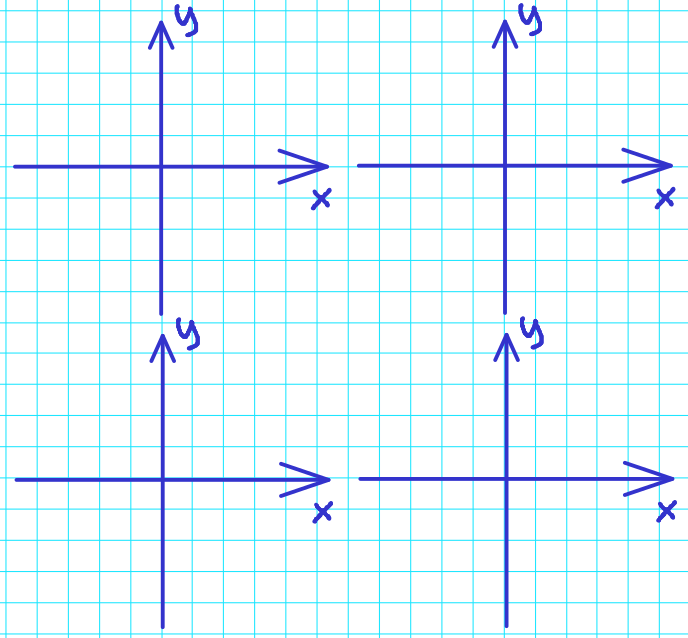
\includegraphics[width=8.5cm]{allg/funktionen/img/potenzfct/potenzFunktionenLeer.png}\hfill{}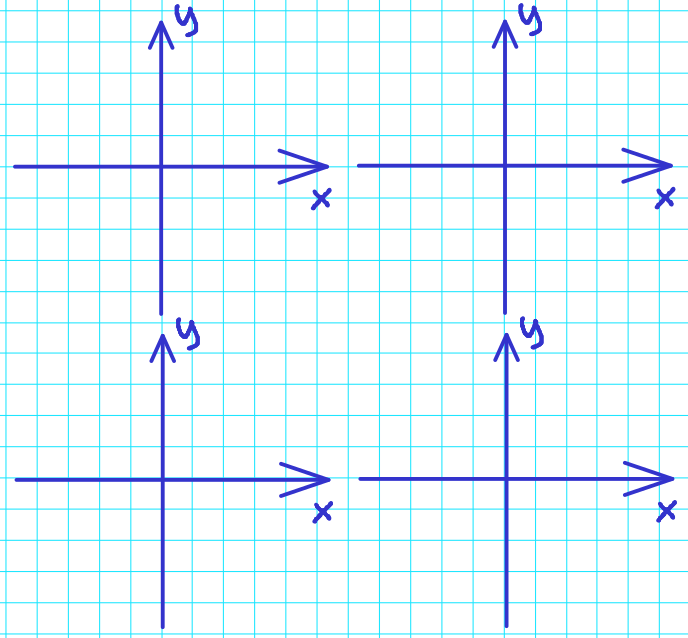
\includegraphics[width=8.5cm]{allg/funktionen/img/potenzfct/potenzFunktionenLeer.png}
}%% END Trainer


\subsection*{Aufgaben}
\AadBMTA{307}{25. b) c), 26. a)\TALS{ b)}, 27. b) c)\TALS{, 33*}}

\newpage


\newpage
\newpage
%%
%% 2019 07 04 Ph. G. Freimann
%%

\section{Exponentialfunktionen}\index{Funktion!Exponentialfunktion}\index{Exponentialfunktionen}
\sectuntertitel{Go viral!}
%%%%%%%%%%%%%%%%%%%%%%%%%%%%%%%%%%%%%%%%%%%%%%%%%%%%%%%%%%%%%%%%%%%%%%%%%%%%%%%%%
\subsection*{Lernziele}

\begin{itemize}
\item Definition Exponentialfunktion
\item Koeffizienten interpretieren
\item Graph: Symmetrien, Polstellen, Asymptoten, Schnittpunkte mit
  Achsen
  \item Basiswechsel
\end{itemize}

\TadBMTA{322}{19}
%%\TALS{(\cite{frommenwiler17alg} S.215 (Kap. 3.10))}
%%\GESO{(\cite{marthaler21alg}       S.322 (Kap. 19))}
\newpage

\subsection{Aussehen von Exponetialfunktionen}


Zeichnen Sie $f: y=2^x$ und $g: y=1.4^x$ ins selbe Koordinatensystem:


\bbwGraph{-5}{5}{-1}{5}{
\TRAINER{  \bbwFuncC{pow(2.0,\x)}{-3.5:2.1}{blue}
  \bbwFuncC{pow(1.4,\x)}{-3.5:3}{green}
  \bbwLetter{1,3}{$f$}{blue}
  \bbwLetter{2.5,2}{$g$}{green}
}%% end TRAINER
}%% end graph

\begin{definition}{Exponentialfunktion}{}\index{Exponentialfunktionen!Definition}
  Eine Funktion der Form $$f(x): x \mapsto a^x$$
  bzw. $$y = a^x$$
  mit $a\in \mathbb{R}^{+}\backslash\{1\}$ heißt \textbf{Exponentialfunktion}.
\end{definition}


\begin{bemerkung}{Zunahmefaktor}{}\index{Zunahmefaktor|textbf}
Der Parameter $a$ gibt den Wachstumsfaktor pro Zeiteinheit $e_x$ an.
\end{bemerkung}


\subsubsection*{Aufgaben}
\GESO{\olatLinkArbeitsblatt{Exponentialfunktionen}{https://olat.bms-w.ch/auth/RepositoryEntry/6029794/CourseNode/106029175831971}{Kap. 1.2:
    Einfache Wachstumsprozesse: Aufgaben 4. bis 6.}}
\TALS{\olatLinkArbeitsblatt{Exponentialfunktionen}{https://olat.bms-w.ch/auth/RepositoryEntry/6029786/CourseNode/106029175777725}{Kap. 1.2:
    Einfache Wachstumsprozesse: Aufgaben 4. bis 6.}}

\newpage

\subsection{Formen der Darstellung}
Zeichnen Sie die Funktionen $f: y=2^x$, $g: y=2^{-x}$ und $h: y=\left(\frac12\right)^x$ in dasselbe Koordinatensystem:

\bbwGraph{-6}{6}{-1}{5}{
  \TRAINER{\bbwFuncC{exp(0.69314718*\x)}{-6:2}{blue}}
  \TRAINER{\bbwFuncC{exp(-0.69314718*\x)}{-2:6}{red} }
  \TRAINER{\bbwLetter{1.5,4}{2^x}{blue}}
  \TRAINER{\bbwLetter{-5,4}{g(x)=2^{-x}=\left(\frac{1}{2}\right)^x=h(x)}{red}}
}

Bemerkung: \TRAINER{$$2^{-x} = \frac1{2^x} = \frac{1^x}{2^x}= \left(\frac12\right)^x$$}
\newpage



\subsubsection{Umkehrung (Optional)}
Um aus einem Wachstum einen Zerfall zu modellieren können wir entweder
die Zeitachse umdrehen oder den Kehrwert der Basis verwenden.
umgedreht werden:

Mit $d := \frac1a $ gilt:

\begin{center}
  \fbox{$a^{+t} = \left(\frac1a\right)^{-t} = d^{-t} $}
\end{center}

\newpage

\newpage

\subsection{Verschiebung und Streckung \GESO{(optional)}}

Eine Verschiebung der Exponentialfunktion $y=b\cdot{}a^x$ in der Zeit ($x$-Richtung) kann auch in Form einer Veränderung der Startfaktors $b$ umgeschrieben werden.

Verschieben wir \zB $$y=2^x$$ um fünf Einheiten nach rechts, so liest sich die neue Funktionsgleichung wie folgt:
$$y=2^{x-5}.$$

(Zeichnen Sie in \texttt{geogebra.org} a) $y=2^x$ und b) $y=2^{x-5}$.)

Dies kann jedoch auch umgeschrieben werden:

$$2^{x-5} = 2^x \cdot{} 2^{-5} = 2^{-5} \cdot{} 2^x = \frac{1}{2^5} \cdot{} 2^x =
\frac{1}{32}\cdot{}2^x$$

\bbwCenterGraphic{8cm}{allg/funktionen/img/exp/verschiebung_gleich_streckung.png}
Bildlegende: Eine Verschiebung ($x$-Richtung) der Exponentialfunktion entspricht einer Stauchung ($y$-Richtung) der selben Exponentialfunktion.

\TALS{Es gilt hier $$a^{x-b}=\frac{a^x}{k}$$ mit
$k=a^b$ und mit $b=\log_a(k)$.}

\newpage


\subsection{Punkte einsetzen\GESO{ (optional)}}
Wie bei den linearen Funktionen oder bei den Potenzfunktionen können auch Exponentialfunktionen gefunden werden, wenn bereits Punkte auf dem Graphen bekannt sind:

\textbf{Referenzaufgabe}

Finden Sie die Parameter $a$ und $b$ der Exponentialfunktion
$$f: y=b\cdot{}a^x$$
wenn Sie wissen, dass die Funktion durch die Punkte $P=(2|4)$ und $Q=(-1|2)$ verläuft:

\TNTeop{
  In Gleichung einsetzen:

  \gleichungZZ{4}{b\cdot{}a^2}{2}{b\cdot{}a^{-1}}

  Einsetzverfahren: Zum Beispiel aus der zweiten Gleichung das $b$ ermitteln...
  $$b = 2 a (III)$$
  ... und in die erste Gleichung einsetzen:

$$4 = 2a\cdot{} a^2$$
  $$2 = a^3$$
  $$a=\sqrt[3]{2}$$
  In (III) einsetzen:

  $$b = 2 \sqrt[3]{2}$$

  Ergo: $$f(x) = b\cdot{}a^x = 2\cdot{}\sqrt[3]{2} \cdot{} \left(\sqrt[3]2\right)^x \approx 2.5198 \cdot{} 1.2599^x$$
}

\subsection*{Aufgaben}
%%\AadBMTA{334}{10. a) b)\TALS{ e)}\GESO{ f)}}
\GESO{\olatLinkArbeitsblatt{Exponentialfunktionen}{https://olat.bms-w.ch/auth/RepositoryEntry/6029794/CourseNode/106029175831971}{Kap. 2.1: E-Funktion / Punkte-Aufgaben Aufg 26. a) b) ($e^{qt}$ optional) und Aufg. 27.}}
\TALS{\olatLinkArbeitsblatt{Exponentialfunktionen}{https://olat.bms-w.ch/auth/RepositoryEntry/6029786/CourseNode/106029175777725}{Kap. 2.1: E-Funktion / Punkte-Aufgaben Aufg 26. a) b) ($e^{qt}$ optional) und Aufg. 27.}}

\AadBMTA{336}{23. d}

\newpage

\newpage
%% 2019 07 04 Ph. G. Freimann
%%

\section{Wachstum und Zerfall}\index{Wachstum}\index{Zerfall}
\sectuntertitel{Sagt ein großer Stift zum kleinen Stift: ``Wachsmalstift!''}

%%%%%%%%%%%%%%%%%%%%%%%%%%%%%%%%%%%%%%%%%%%%%%%%%%%%%%%%%%%%%%%%%%%%%%%%%%%%%%%%%

\TRAINER{
  Video \href{https://www.youtube.com/watch?v=TMaLuks8dxw}{MatheMann}
Wo schneiden sich $x^3$ und $e^x$?}%%
\subsection*{Lernziele}

\begin{itemize}
\item Zinseszins
\item Wachstums-, Zerfallsprozesse
\item Verdoppelungs- und Halbwertszeiten
%%\item Basiswechsel
\end{itemize}

\TadBMTA{342}{20}
%%\TALS{(\cite{frommenwiler17alg} S.221 (Kap. Exponentielles Wachstum))}
%%\TALS{(\cite{frommenwiler17alg} S.223 (Kap. Exponentielle Abnahme))}
%%\TALS{(\cite{frommenwiler17alg} S.225 (Kap. Zinseszins))}
%%\GESO{(\cite{marthaler21alg}       S.342 (Kap. 20))}

\newpage


\subsection{Beispiele}
Bei Wachstumsprozessen sprechen wir dann von einer exponentiellen
Zunahme, wenn die Zunahme pro Zeiteinheit immer proportional zum aktuellen Bestand ist.

\begin{itemize}
\item \Lueckentext{Zinseszins}
\item \Lueckentext{Frequenzen in der temperierten Stimmung
  (Musik). Zunahme der Frequenz pro Halbtonschritt.}
\item \Lueckentext{Keime in der Kuhmilch; Ansteckungsbedingte Krankheitsfälle (\zB viral)}
\item \Lueckentext{Algenbefall in Teichen}
\item \Lueckentext{Generell Populationen: Flechten, Pilze}
\item \Lueckentext{(ungebremstes) Bevölkerungswachstum / bzw. Tierpopulation}
\item \Lueckentext{\dotfill}
\end{itemize}


\GESO{\olatLinkArbeitsblatt{Exponentialfunktionen}{https://olat.bms-w.ch/auth/RepositoryEntry/6029794/CourseNode/106029175831971}{Kap. 1.1:
    Voraussetzungen: Aufgaben 1. bis 3.}}
\TALS{\olatLinkArbeitsblatt{Exponentialfunktionen}{https://olat.bms-w.ch/auth/RepositoryEntry/6029786/CourseNode/106029175777725}{Kap. 1.1:
    Voraussetzungen: Aufgaben 1. bis 3.}}


\newpage

\subsection{Einstiegsbeispiel Taschengeld}

Bei Familie Cash kann man aussuchen, wie sich sein Taschengeld über
die Jahre «vermehrt». Mani wählt Variante A. Bei Varante A erhält man
CHF 1.- im ersten Jahr, CHF 2.- im 2. Jahr, CHF 3.- im 3. Jahr und so
weiter bis zur abgeschlossenen Grundbildung im 13. Jahr CHF 13.-.

Carla wählt Variante B. Bei der Variante B erhält Carla auch CHF 1.-
im ersten Jahr, dann aber jedes Jahr 30\% mehr, als im Vorjahr.

a) Wird Carla vor Ende der Grundbildung jemals mehr als Mani erhalten?

\LoesungsRaumLang{Ja, im 10. Schuljahr}

b) Wer hat über alle Jahre mehr Taschengeld?

\LoesungsRaumLang{Carla wird mehr haben}

c) Skizzieren Sie beide Varianten:

\TRAINER{\bbwCenterGraphic{13cm}{allg/funktionen/img/taschengeldAusgefuellt.png}}
\noTRAINER{\bbwCenterGraphic{16cm}{allg/funktionen/img/taschengeld.png}}

\TRAINER{Optional: Zeige mit Geogebra (\texttt{geogebra.org}) $x^2$ vs. $1.2^x$. Fazit:
  Exponentielles Wachstum überholt jegliche Potenzfunktion.}



\newpage

Zeichnen Sie $f: y=2^x$ und $g: y=1.4^x$ ins selbe Koordinatensystem:


\bbwGraph{-5}{5}{-1}{5}{
\TRAINER{  \bbwFuncC{pow(2.0,\x)}{-3.5:2.1}{blue}
  \bbwFuncC{pow(1.4,\x)}{-3.5:3}{green}
  \bbwLetter{1,3}{$f$}{blue}
  \bbwLetter{2.5,2}{$g$}{green}
}%% end TRAINER
}%% end graph

\begin{definition}{Exponentialfunktion}{}\index{Exponentialfunktionen!Definition}
  Eine Funktion der Form $$f(x): x \mapsto a^x$$
  bzw. $$y = a^x$$
  mit $a\in \mathbb{R}^{+}\backslash\{1\}$ heißt \textbf{Exponentialfunktion}.
\end{definition}


\begin{bemerkung}{Wachstumsfaktor}{}\index{Wachstumsfaktor}
Der Parameter $a$ gibt den Wachstumsfaktor pro Zeiteinheit $e_x$ an.
\end{bemerkung}


\subsubsection*{Aufgaben}
\GESO{\olatLinkArbeitsblatt{Exponentialfunktionen}{https://olat.bms-w.ch/auth/RepositoryEntry/6029794/CourseNode/106029175831971}{Kap. 1.2:
    Einfache Wachstumsprozesse: Aufgaben 4. bis 6.}}
\TALS{\olatLinkArbeitsblatt{Exponentialfunktionen}{https://olat.bms-w.ch/auth/RepositoryEntry/6029786/CourseNode/106029175777725}{Kap. 1.2:
    Einfache Wachstumsprozesse: Aufgaben 4. bis 6.}}


\newpage

\subsection{Exponentieller Zerfall}\label{zerfallsfunktion}
Die Funktion $f(x): x \mapsto y = d^{-x}$ ist eine
Exponentialfunktion, die gegen Null geht.

\bbwFunction{-4}{4}{-1}{8}{exp(-\x)}{-2:4}

\begin{bemerkung}{}{}
Oft wird bei Wachstumsprozessen die Zeitachse auch mit $t$ statt $x$ bezeichnet: $t$ steht für \textit{time}.
\end{bemerkung}

\newpage

\subsubsection{Beispiele}
\begin{itemize}
	\item \Lueckentext{Zinsliche Abschreibungen (\zB Wert eines Autos)}
	\item \Lueckentext{Radioaktiver Zerfall}
	\item \Lueckentext{Lichtintensität in Medium (Gas / Flüssigkeit / Glasfaser), dies gilt vertikal, wie auch horizontal}
	\item \Lueckentext{Atmosphärischer Luftdruck in Metern über Meer}
  \item \Lueckentext{Entladen einer Batterie bzw. eines Kondensators}
  \item \Lueckentext{Sauerstoffkonzentration in Seen (\zB Herbst bei kontinuierlicher Abnahme)}
  \item \Lueckentext{Abnahme des Bierschaums im Glas}
  \item \Lueckentext{Mischen, wie im Sirup-Beispiel\totalref{sirup_beispiel}}
  \item \Lueckentext{«Halbwertszeit des Wissens» ;-)}
  \item \Lueckentext{\dotfill}
\end{itemize}

\newpage



Zeichnen Sie die Funktionen $f: y=2^x$, $g: y=2^{-x}$ und $h: y=\left(\frac12\right)^x$ in dasselbe Koordinatensystem:

\bbwGraph{-6}{6}{-1}{5}{
  \TRAINER{\bbwFuncC{exp(0.69314718*\x)}{-6:2}{blue}}
  \TRAINER{\bbwFuncC{exp(-0.69314718*\x)}{-2:6}{red} }
  \TRAINER{\bbwLetter{1.5,4}{2^x}{blue}}
  \TRAINER{\bbwLetter{-5,4}{g(x)=2^{-x}=\left(\frac{1}{2}\right)^x=h(x)}{red}}
}

Bemerkung: \TRAINER{$$2^{-x} = \frac1{2^x} = \frac{1^x}{2^x}= \left(\frac12\right)^x$$}
\newpage

\subsubsection{Grundform} \index{Exponentieller Prozess! Grundform}
Die Grundform für Zerfallsprozesse lautet:

\begin{definition}{Zerfall}{}\index{Zerfall}
  Die Grundform des exponentiellen Zerfalls wird beschrieben durch die Funktion
$$f(x): x \mapsto a^x$$
  bzw.
  $$y = a^x$$
\end{definition}


\begin{gesetz}{Wachstum vs. Zerfall}{}

  Der einzige Unterschied bei Wachstums- bzw Zerfallsprozessen ist der
  Faktor $a$:

  \begin{itemize}
    \item \LoesungsRaumLen{40mm}{$a>1$: Wachstum}\vspace{3mm}
    \item \LoesungsRaumLen{40mm}{$0<a<1$: Zerfall}
  \end{itemize}
  
\end{gesetz}

\begin{bemerkung}{$x$-Richtung}{}
  Exponentielle Prozesse laufen meist in der Zeit ab. Somit wird
  die $x$-Achse zur Zeitachse und meist mit $t$ (Time) bezeichnet:
  $$f(t) = a^t$$
  \end{bemerkung}


\subsubsection{Umkehrung (Optional)}
Um aus einem Wachstum einen Zerfall zu modellieren können wir entweder
die Zeitachse umdrehen oder den Kehrwert der Basis verwenden.
umgedreht werden:

Mit $d := \frac1a $ gilt:

\begin{center}
  \fbox{$a^{+t} = \left(\frac1a\right)^{-t} = d^{-t} $}
\end{center}

\newpage

\subsection*{Aufgaben}
%%\TALSAadBMTA{223ff}{840., 841., 843., 844. und 846.}

\GESO{\olatLinkArbeitsblatt{Exponentialfunktionen}{https://olat.bms-w.ch/auth/RepositoryEntry/6029794/CourseNode/106029175831971}{Kap. 1.3: Zerfall: Aufg. 7., 8. und 9.}}
\TALS{\olatLinkArbeitsblatt{Exponentialfunktionen}{https://olat.bms-w.ch/auth/RepositoryEntry/6029786/CourseNode/106029175777725}{Kap. 1.3: Zerfall: Aufg. 7. 8. und 9.}}

\AadBMTA{354}{9. (Bauchspeicheldrüse)}
\olatLinkGESOKompendium{3.4.1}{27ff}{33., 35., 36., 39. und 41.}

\newpage
%% Sirup-Beispiel
\subsection{Mischtank}\index{Mischtank}\index{Sirup}\label{sirup_beispiel}
Wird ein Glas Wasser in ein Glas Sirup geschüttet, so

\TRAINER{\bbwCenterGraphic{5cm}{allg/alg/potenzen_wurzeln/img/Schwapp.png}}%%
\noTRAINER{\bbwCenterGraphic{5cm}{allg/alg/potenzen_wurzeln/img/SchwappOhneFormel.png}}

geschieht erst mal etwas eher klebriges:
\begin{itemize}
  \item Das Wasser verdrängt den Sirup und
  \item das Sirupglas schwappt über.
\end{itemize}

Wenn man nun gleichzeitig im Sirupglas
umrührt, so mischt sich das Wasser mit dem Sirup und je länger man
Wasser einschüttet, umso verdünnter wird der Sirup.


Wie viel Sirup bleibt im Glas?

\TNT{2.4}{
Am Ende bleibt ein
Verhältnis von Wasser : Sirup = $\left(1-\frac{1}{e}\right) : \left(\frac{1}{e}\right)$
\vspace{1.5cm}
}

Diese Konstante wird oft in großen chemischen Mischtanks verwendet,
gibt aber auch ein Maß an, wenn \zB in einer Minergie-Wohnung die Luft
ausgetauscht wird. Wenn nämlich das Volumen der Wohnung einmal neu hineingepumpt (bzw. weggeblasen) wurde während sich alte die Luft im Haus permanent mit der neuen vermischt, so ist noch ein Anteil von \TRAINER{$\frac{1}{e}$}\noTRAINER{ ..... } der alten Luft im Haus.
\newpage


\textbf{Begründung:}\\
1. Gedanke: Jedes eingefüllte Glas, vermindert die vorhandene
Sirupkonzentration um den selben Faktor. Ergo handelt es sich um
einen exponentiellen Zerfall.

\leserluft

2. Gedanke: Wir tauschen drei Mal $\frac13$ aus. Nehmen also im
\begin{itemize}
\item \textbf{ersten Schritt} $\frac13$ des Sirups weg (und ersetzen diesen mit Wasser).
  Es bleiben $\frac23$ Sirup. Den Rest füllen wir mit Wasser auf.
\item Im \textbf{zweiten Schritt} nehmen wir $\frac13$ des Gemisches
weg; es verbleiben also $\frac23$ von $\frac23$ an
Sirup-Konzentrat. Der Rest wird immer wieder mit Wasser aufgefüllt. Mit
anderen Worten: Es bleiben $\frac23 \cdot \frac23
= \left(\frac23\right)^2$ an Sirup\footnote{Man könnte hier auch argumentieren mit: «Wir nehmen von den $\frac23$ einen Drittel weg»: $\frac23 - (\frac13$ von $\frac23)$ = $\frac23 - (\frac13 \cdot\frac23) = \frac23 \cdot(1-\frac13)=\frac23\cdot\frac23$}.
\item Im \textbf{dritten Schritt} entnehmen wir wieder $\frac13$ des
Gemisches; es verbleiben wieder $\frac23$ vom bisherigen Sirup, also
$\frac23$ von $(\frac23)^2$ also $\left(\frac23\right)^3$.

Beim dreistufigen Gedankenexperiment verbleiben
$\left(\frac23\right)^3 = \left(1-\frac13\right)^3$ der ursprünglichen Konzentration.
\end{itemize}
\leserluft

3. Gedanke: Das Experiment vom vorherigen Gedanken können wir natürlich auch mit immer kleineren\TALS{, sogenannten infinitesimalen,} Schritten durchführen.
Mit Centilitern \zB im dl-Glas ersetzen wir 10 Mal je $\frac1{10}$. 
So verbleibt am Schluss $\left(1-\frac{1}{10}\right)^{10}\approx 0.35$ Sirup.

\GESO{Wenn wir (\zB mit dem Taschenrechner) die Schrittanzahl immer weiter vergrößern (und somit die pro Schritt ausgetauschte Menge immer verkleinern), so ergibt sich für 1000 Schritte ein Verhältnis von $\left(1-\frac{1}{1000}\right)^{1000}\approx 0.3677 \approx \frac1{\e}$. }
\TALS{Wenn wir die Schritte permanent erhöhen (und gegen Unendlich gehen lassen), so erhalten wir den Grenzwert (lat. Limes) von

$$\lim_{n\rightarrow\infty} \left(1-\frac{1}{n}\right)^n = \frac1{\e}$$
}
\newpage

\textbf{Aufgabe 1: Sirup}\\
Wie viel Wasser muss eingeschüttet werden, damit das auf der Flasche
angegebene Verhältnis von 1:6 (1 Teil Sirup, 6 Teile Wasser) zustande
kommt?

\TNT{8}{
Bei 1x Schütten, erhalten wir $\left(\frac{1}{\e}\right)^1$ Anteil Sirup.

Bei 2x Schütten, erhalten wir $\left(\frac{1}{\e}\right)^2$ Anteil Sirup.

Somit erhalten wir den Siebtel (1:6 = $\frac17$-Anteil) indem wir die
folgende Exponentialgleichung lösen:

$$\frac17 = \left(\frac{1}{\e}\right)^n$$
Diese Gleichung lösen wir, indem wir beidseitig logarithmieren und so
erhalten wir den einzuschüttenden Teil $$n=\ln(7)\approx{1.946}.$$
}%% END TNT

\textbf{Aufgabe 2: Minerige-Haus}\\
Wenn wir also wissen wollen, wie viel Luft in ein Minergiehaus
eingepumpt werden muss, damit nur noch 1 Promille der alten Luft
vorhanden ist, so erhalten wir
\TNTeop{
  $$\text{Volumen Neuluft} = \text{Wohnungsvolumen}\cdot{}\ln(1000)$$
  $$\ln(10000) \approx 6.9$$
} %% end TNT


\newpage

\newpage


\subsection{Startwert}\index{Startwerte!bei Wachstums- und Zerfallsprozessen}

Die bisher betrachteten Exponentialfunktionen haben für den Wert $x=0$ (bzw. $t=0$) immer den
$y$-Wert = 1 bzw. 100\%.
Da in der Praxis meist konkrete Werte vorgegeben sind verwenden wir
eine \textbf{allgemeinere Form der Exponentialfunktion}.

\subsubsection{Einstiegsbeispiel}

\begin{beispiel}{Pilz}{}
  Ein Pilzbefall an einer Wand nehme täglich um 23\% der Fläche
  zu\footnote{Je nach Organismus ist auch ein quadratisches Wachstum
  vorhanden, doch für unser Experiment verwenden wir exponentielles Wachstum.}.
  Anfänglich wird eine Fläche von $35$ $\text{cm}^2$ gemessen.
  Welche Fläche ist nach einem, nach zwei, nach fünf, nach zehn
  bzw. nach $n$ 
  Tagen zu erwarten?

  \TNT{6}{Ein  Tag:   $35\cdot{} 1.23^1    =          43.05 \text{cm}^2$\\
          Zwei Tage:  $35\cdot{} 1.23^2   \approx{}  52.95 \text{cm}^2$\\
          Fünf Tage:  $35\cdot{} 1.23^5   \approx{}  98.54 \text{cm}^2$\\
          Zehn Tage:  $35\cdot{} 1.23^{10} \approx{} 277.4 \text{cm}^2$\\
          $n$  Tage:  $35\cdot{} 1.23^n = 35\cdot{}1.23^n$}%% END TNT

  Wann wird die ganze Wand ($6 \text{ m}^2$) mit dem Pilz befallen
  sein?
  
\TNT{6}{$6 \text{ m}^2 = 60\,000 \text{ cm}^2$
     
     ergo: $60\,000 = 35 \cdot{} 1.23^n$

     (durch 35 teilen, dann logarithmieren)

     $$\frac{60\,000}{35} = 1.23^n$$

     $$n = \log_{1.23}\left(\frac{60\,000}{35}\right) \approx 35.97 \text{Tage}$$

   }%% END TNT

\end{beispiel}

\newpage


\begin{gesetz}{Exponentialfunktion mit frei wählbarem Startwert}{}
$$f: y = \LoesungsRaumLen{40mm}{b\cdot{}a^x}$$

Auch hier gibt der Parameter $a$ den Wachstumsfaktor pro Zeiteinheit $e_x$ an.

Dabei ist $b$ der Startwert zum Zeitpunkt $x$ = 0.
\end{gesetz}


\noTRAINER{\bbwCenterGraphic{8cm}{allg/funktionen/img/exp/b_faktor.png}}
\TRAINER{\bbwCenterGraphic{8cm}{allg/funktionen/img/exp/b_faktor_trainer.png}}

\begin{bemerkung}{Wachstumsfaktor}{}{}
Werden zwei $x$ Positionen mit Differenz 1 (=$e_x$) betrachtet, so sind
die zugehörige $y$-Werte um \textbf{Faktor} $a$ auseinander.
\end{bemerkung}

Begründung:
\TNTeop{
  Gegeben $x_1$ und $x_2 = x_1 + 1$. So ist

  $y_1 = b\cdot{}a^{x_1}$ und $y_2 = b\cdot{}a^{x_2}$.

  Setzen wir nun $x_1 + 1$ für $x_2$ ein, so erhalten wir:

  $$y_2 = f(x_2) = b\cdot{}a^{x_2} = b\cdot{} a^{x_1+1} =  b\cdot{}a^{x_1} \cdot{} a^1 = y_1\cdotp{} a$$
}
\newpage


\subsection*{Aufgaben}

\GESO{\olatLinkArbeitsblatt{Exponentialfunktionen}{https://olat.bms-w.ch/auth/RepositoryEntry/6029794/CourseNode/106029175831971}{Kap. 1.4:
    Frei wählbarer Startwert: Aufg. 10. Gummiball; 11. Neophytenplage;
    12: Tierpopulation; 13. Licht im Wasser;  weitere Aufgaben 14. bis 17.}}
\TALS{\olatLinkArbeitsblatt{Exponentialfunktionen}{https://olat.bms-w.ch/auth/RepositoryEntry/6029786/CourseNode/106029175777725}{Kap. 1.4:
    Frei wählbarer Startwert: Aufg. 10. Gummiball; 13. Licht im Wasser. 14. Federpendel; 15. Luftdruck; weitere Aufgaben aus
    Kap. 1.4.}}
 
  \AadBMTA{338}{29. (Bierschaum)}
  \AadBMTA{353}{6. (C-14 Methode)}

  Als Vorbereitung zur allgemeinen Wachstumsfunktion:
  \AadBMTA{207}{10. (Algen)}

\newpage


\subsection{Beobachtungszeitspanne}
\subsubsection{Einstgiesbeispiel}
\bbwCenterGraphic{17cm}{allg/funktionen/img/tuerlersee2.jpg}
\begin{center}{\small Legende: Türlersee April 2022}\end{center}

Der Türlersee ist ein kleiner See im Reppischtal. Seine Oberfläche
begann sich vor einigen Jahrzehnten stark mit Algen\footnote{Genau
  genommen handelte es sich um Zooplanktonbiomasse zwischen 1982 und 1994, doch als
  Idee zur Exponentialfunktion sollte ein ungefähres Flächenmodell reichen.} zu bedecken.

Anfänglich (zum Zeitpunkt $t=0$) waren gerade mal 20$m^2$ bedeckt. Doch nach fünf Tagen hatte sich diese Fläche verdoppelt und nach weiteren fünf Tagen nochmals verdoppelt (also insgesamt vervierfacht).

Füllen Sie die (prognostizierte) Wertetabelle für 30 Tage ein:

\def\spaceX{\,\,\,\,\,\,\,\,\,\,}
\newcommand\tuerlerB[1]{\noTRAINER{\spaceX}\TRAINER{#1}}
\begin{tabular}{l|c|c|c|c|c|c|c}
  $t$:  & 0 & 5 & 10 & 15 & 20 & 25 & 30 \\
  \hline
  $m^2$ & \tuerlerB{20}  & \tuerlerB{40}  &   \tuerlerB{80}  &  \tuerlerB{160}  &  \tuerlerB{320}  &  \tuerlerB{640}  &  \tuerlerB{1280} \\
\end{tabular}

\newpage
Zeichnen Sie die Algenpopulation als Graph in eine Koordinatensystem
(beginnen Sie mit dem Ursprung ganz links unten. $x$-Achse in Tagen ($t$). $y$-Achse in $\text{m}^2$.

\noTRAINER{\bbwCenterGraphic{170mm}{allg/funktionen/img/exp/WachstumTuerlerseeLeer.png}}
\TRAINER{\bbwCenterGraphic{10cm}{allg/funktionen/img/exp/tuerlerAlgen.png}}
\newpage

\textbf{Funktionsgleichung}

Wir betrachten die selbe Algenpopulation mit einer
Ver\textbf{\color{blue}dopplung} der Fläche alle \textbf{\color{red}fünf} Tage bei einer
Startfläche von \textbf{\color{green}zwanzig} $\text{m}^2$.

Geben Sie eine Funktionsgleichung an, welche das Wachstum der
Algenpopulation beschreibt...



\begin{bbwFillInTabular}{c|c|c||c|c|c|c|c|c|c|c}\hline
  Tage      & $t$ & \cellcolor{gray!75}\noTRAINER{\hspace{2cm}} & 0            & \tiny{1-4} & 5            & \tiny{6-9} & 10           & \tiny{11-14} & 15           &\\\hline
  Fläche     & $A$ & \TRAINER{$20\cdot v$}    &
  \TRAINER{20}\noTRAINER{\hspace{15mm}} &  \cellcolor{gray!75}    &
  \TRAINER{40}\noTRAINER{\hspace{15mm}} &    \cellcolor{gray!75}  &
  \TRAINER{80}\noTRAINER{\hspace{15mm}} &         \cellcolor{gray!75}       &
  \TRAINER{160}\noTRAINER{\hspace{15mm}} &\\\hline
  Faktor    & $v$ & \TRAINER{$v=2^z$}    & \TRAINER{1}  &  \cellcolor{gray!75}    & \TRAINER{2}  &   \cellcolor{gray!75}   & \TRAINER{4}  &    \cellcolor{gray!75}            & \TRAINER{8} &\\\hline
  Intervalle & $z$ & \TRAINER{$z=\frac{t}{5}$}    & \TRAINER{0}  &  \cellcolor{gray!75}    & \TRAINER{1.}  & \cellcolor{gray!75}     & \TRAINER{2.}  &   \cellcolor{gray!75}             & \TRAINER{3.} &\\\hline
  Potenz     &\TRAINER{$2^z$} & \TRAINER{$2^\frac{t}{5}$}     & \TRAINER{$2^0$}  &   \cellcolor{gray!75}   & \TRAINER{$2^1$}  &   \cellcolor{gray!75}   & \TRAINER{$2^2$}  &  \cellcolor{gray!75}              & \TRAINER{$2^3$} &\\\hline
\end{bbwFillInTabular}

\TRAINER{Falls nicht mit Tabelle: 1. Tipp $f(0)=20; f(5)=40;
  f(10)=80;...$, dann 2. Tipp $f_B(0) = 20; f_B(1)=40; ...$ $B$=Anzahl
  Beobachtungsintervalle}

\leserluft
\begin{center}
  $f(t):\,\,\, y=\LoesungsRaumLang{{\color{green}20}\cdot{} {\color{blue}2} ^{\frac{t}{\color{red}5}}}$
  \end{center}
\TNT{4}{
Dabei bezeichnet\\20 den Startwert,\\2 den Zunahmefaktor und \\5 die Beobachtungszeitspanne.}%%

Merke:
\TNTeop{Ich muss für $t$ fünf Tage einsetzen, um auf eine Verdopplung
  zu kommen.

  Setze ich $t=0$ ein, so erhalte ich den Startwert zwanzig m$^2$.
}
%%%%%%%%%%%%%%%%%%%%%%%%%%%%%%%%%%%%%%%%%%%%%%%%%%%%%%%%%%%%%%%%%%%%%%%%%%%%%%%%%%%%%%%%%%%%%%%%%%%%

\subsubsection{Exponentieller Prozess (allgemein)}\index{Exponentieller Prozess! allgemeine Form}

\begin{gesetz}{Wachstumsprozess}{}
  Die Funktion

  $$y = f(t) = \LoesungsRaumLen{40mm}{b\cdot{}a^{\frac{t}{\tau}}}$$
  
  beschreibt einen allgemeinen exponentiellen Wachstumsprozess mit
  $$   a=\LoesungsRaumLen{50mm}{\text{Wachstumsfaktor während } \tau \text{ Tagen} }$$
  $$   b=\LoesungsRaumLen{50mm}{\text{Startwert}}$$
  $$\tau=\LoesungsRaumLen{50mm}{\text{Beobachtungszeitspanne}}$$
\end{gesetz}

Alternativ «die harte Tour» (ohne das $\tau$ mit anderer Basis):

\TNTeop{


  $$f(t) = b\cdot{}A^t$$

  $A$ = Faktor pro Tag, $t$ = Anzahl Tage, Startwert $b=f(0)$
  
  Bsp.: Die Algenzahl verdoppelt sich alle fünf Tage:

  $$f(5)        = 2 \cdot{} f(0)$$
  $$b\cdot{}A^5 = 2 \cdot{} b $$

  $$A^5 = 2$$

  $$A = \sqrt[5]{2} = 2^{\frac15} \approx 1.1487$$

  Einsetzen in $f(t) = b\cdot{} A^t$

  $$f(t) = b\cdot{} \left(\sqrt[5]{2}\right)^t  = b\cdot{}
  \left(2^{\frac15}\right)^t=b\cdot{} 2^{\frac{t}5} \approx b\cdot{} 1.1487^t$$

}%% end TNTeop


\newpage

\subsubsection{Graphische Erläuterung (optional)}


\begin{tabular}{cc}%%
  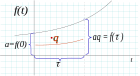
\includegraphics[width=9cm]{allg/funktionen/img/exp/exponentielles_wachstum.png} &
  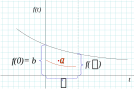
\includegraphics[width=7cm]{allg/funktionen/img/exp/exponentieller_zerfall.png}\\
\end{tabular}

%%\bbwCenterGraphic{10cm}{allg/funktionen/img/exp/exponentieller_zerfall.png}
%%\bbwCenterGraphic{11cm}{allg/funktionen/img/exp/exponentielles_wachstum.png}

Dabei sind
\begin{itemize}
\item $b=f(0)$ der Anfangsbestand zum Zeitpunkt $t$ = 0.
\item $\tau$ ist die typische Zeitspanne zwischen zwei Beobachtungszeitpunkten (zum Beispiel zwischen Wert und dessen Verdopplung). Beispiele:
  \begin{itemize}
  \item Verdoppeln in 3 Stunden: $a=2$ und $\tau = 3\, \text{h}$
    ($\text{h}$ = Stunden)
  \item Verfünf"|fachen einer Viertelstunde (= 15 Minuten): $a=5$ und
    $\tau=\frac{1}{4}\, \text{h}$
  \end{itemize}
  Meist ist die Beobachtungszeit gleichzeitig die Maßeinheit (\zB
  Veränderung pro Stunde). Dann ist unser $\tau=1$ und die Formel
  vereinfacht sich zu $f(t) = b\cdot{}a^t$.
\item $a$ ist der Zunahmefaktor zwischen zwei Beobachtungszeitpunkten (Beispiel $a=2$ bei Verdoppelungsprozessen).
  $a$ berechnet sich durch den Quotienten zwischen zwei
  Beobachtungswerten $a = \frac{f(\tau)}{f(0)} =\frac{m}{b}$.
\item
  Dabei ist $m$ der Messwert zum Zeitpunkt $\tau$.
\item $f(t)=b\cdot{}a^{\frac{t}{\tau}}$ ist der Wert (Anzahl, Fläche,
  Bestand, ...) zum Zeitpunkt
  $t$. 
\end{itemize}

Bemerkung: 
\TNTeop{
$\frac{m}b = \frac{f(\tau)}{f(0)}=\frac{b\cdot{}a^{\frac{\tau}{\tau}}}{b\cdot{}a^{\frac0{\tau}}}
  = \frac{a^1}{a^0} = \frac{a}{1} 
  = a$}%% END TNT
\newpage

\subsection{Referenzaufgabe}\index{Irland!Bevölkerungswachstum}
Irland hatte 1990 3.51 Mio. Einwohner. Im Jahr 2019 waren es bereits 4.93 Mio.

\textbf{Frage 1}: Was prognostizieren Sie für das Jahr 2025, wenn Sie von einem exponentiellen Wachstum ausgehen?

\noTRAINER{\bbwCenterGraphic{12cm}{allg/funktionen/img/exp/IrlandLeer.png}}%%

\TNTeop{
  Skizze:
  \bbwCenterGraphic{12cm}{allg/funktionen/img/exp/IrlandVoll.png}

  $\tau$ = 29 Jahre, Einheit = Jahre ($t$ in Jahren gemessen).
  
  $b=f(0) = 3.51$ [Mio EW] = Startwert (Taschenrechner STO).

  $m=f(\tau) = 4.93$ [Mio EW] = Messwert nach $\tau$ Jahren.

  $a=\frac{m}{b}=\frac{4.93}{3.51} \approx 1.4046$ pro 29 Jahre (Taschenrechner! STO). 

  $$f(t) = b\cdot{}a^\frac{t}{\tau}=b\cdot{}a^\frac{t}{29}$$


  TR Probe $b\cdot{}a^\frac{0}{29} = ? = 3.51$ 

  TR Probe $b\cdot{}a^\frac{29}{29} = ? = 4.93$ 

  Jahr 2025: $t=35$:

    $$f(35) = b\cdot{}a^\frac{35}{29}\approx 5.28899$$

}%% END TNT
\newpage

\subsection*{Aufgaben}

\GESO{\olatLinkArbeitsblatt{Exponentialfunktionen}{https://olat.bms-w.ch/auth/RepositoryEntry/6029794/CourseNode/106029175831971}{Kap. 1.5: Aufg. 18. a) b)}}
\TALS{\olatLinkArbeitsblatt{Exponentialfunktionen}{https://olat.bms-w.ch/auth/RepositoryEntry/6029786/CourseNode/106029175777725}{Kap. 1.5:     Aufg. 18. a) b) }}

\newpage

\textbf{Frage 2}: In wie vielen Jahren hat sich die Bevölkerung verdreifacht?

\TNTeop{
  Gesucht $T_3$ = Verdreifachungszeitpunkt.

  $$f(T_3) = 3\cdot{}f(0)$$

  Funktionsgleichung einsetzen:

  $$b\cdot{}a^\frac{T_3}{\tau} = 3\cdot{} b\cdot{} a^\frac0\tau$$

  Weil $a^{\frac{0}{\tau}} = 1$ folgt:

  $$b\cdot{}a^\frac{T_3}{\tau} = 3\cdot{} b$$

  $$a^\frac{T_3}{\tau} = 3$$

  Def. Logarithmus:

  $$\frac{T_3}{\tau} = \log_a(3)$$

$$T_3 = \tau\cdot{}\log_a(3) = 29\cdot{}\log_a(3) \approx 93.8$$
Die Bevölkerung wird sich voraussichtlich alle 94 Jahren
verdreifachen.

}%% END Trainer
\newpage

\subsection*{Aufgaben}
%%\TALSAadBMTA{221ff}{831 - 839}


\GESO{\olatLinkArbeitsblatt{Exponentialfunktionen}{https://olat.bms-w.ch/auth/RepositoryEntry/6029794/CourseNode/106029175831971}{Kap. 1.5:
    Aufg. 18. c), 19. - 21.}}
\TALS{\olatLinkArbeitsblatt{Exponentialfunktionen}{https://olat.bms-w.ch/auth/RepositoryEntry/6029786/CourseNode/106029175777725}{Kap. 1.5:
    Aufg. 18. c), 19. - 21. }}

\AadBMTA{338}{28. Bakterien}
\AadBMTA{352ff}{2. (Hasenpopulation), 7., 1. (optional)}
\olatLinkGESOKompendium{3.4}{27ff}{32., 34., 38., 40., 44., 45. und 46.}
\GESO{\aufgabenFarbe{Nullserie 2: Aufgabe 8.}}
\GESO{\aufgabenFarbe{Maturaprüfung 2017, Aufg. 12 (Raupen)\\
Maturaprüfung 2018 (Serie 3), Aufg. 11 (Müll)
}}



%% TODO Arbeitsblatt verlinken
%%\GESO{\olatLinkArbeitsblatt{Exponentialfunktionen}{https://olat.bms-w.ch/auth/RepositoryEntry/6029794/CourseNode/106029175831971}{Kap. 1.1: Voraussetzungen}}
%%\TALS{\olatLinkArbeitsblatt{Exponentialfunktionen}{https://olat.bms-w.ch/auth/RepositoryEntry/6029786/CourseNode/106029175777725}{Kap. 1.1: Voraussetzungen}}



\newpage

\subsection{Rate vs. Faktor
  II}\index{Rate}\index{Fatkor}\index{Zunahmefaktor}\index{Zunahmerate}
\totalref{RateZins1}

Den Unterschied von Zinsfuß (= Rate) und Zinsfaktor kennen wir bereits aus der Zinsrechnung.

So entspricht eine Zunahme von 12\% einem\\
Aufzinsungsfaktor von \LoesungsRaumLang{1.12}.

Wenn jedoch eine Beobachtung einer Zunahme von, sagen wir, 70\% innerhalb einer Viertelstunde beobachtet wird, so können wir uns fragen, um wie viel die Zunahme (als Rate oder Faktor) pro Zeiteinheit (hier Stunden) ist.


Füllen Sie dazu folgende Tabelle aus. Dabei bedeuten

\begin{tabular}{lp{14cm}}\hline
  Einheit & Stunden, Minuten, Meter, ... \\\hline
  $\tau$  & In dieser Zeitspanne (Stunden, Meter, ...) wird beobachtet \\\hline
  $p$     & Zunahme\textbf{rate}\index{Zunahmerate}\index{Rate} während $\tau$ Einheiten in \%. Ist $p$ negativ, handelt es sich um eine Abnahme\\\hline
  $a_\tau$ & Zunahme\textbf{faktor}\index{Zunahmefaktor} während $\tau$ Einheiten. Ist $a<1$, handelt es sich um einen Abnahmefaktor\\\hline
  $a_E$ (Formel)   & Zunahme pro Einheit (als Faktor). Aufgeschrieben als Formel\\\hline
  $\approx a_E$ (Zahl)  & Zunahme pro Einheit (als Näherungswert).\\\hline
  $p_E$   & Prozentuale Zunahme pro Zeiteinheit\\\hline
  \end{tabular} 

\leserluft{}
\leserluft{}
%% temporäres Platzhalterchen 
\newcommand{\ph}[1]{\noTRAINER{...........}\TRAINER{#1}}

%%\renewcommand{\arraystretch}{1.7}
$$f(t) = a_\tau^{\frac{t}\tau} = a_E^t$$
%% probably turn off auto-fill-mode in emacs when editing long lines
\begin{bbwFillInTabular}{|l|l|l|l|l|l|l|}\hline
  Einheit & $\tau$            &  $p$         & $a_\tau$         & $a_E$ (Formel)           &  $\approx a_E$    &$p_E$            \\\hline\hline
  h       &  $3$              &  56\%        & $1.56$           & $1.56^\frac13$            &  1.1598           & 11.598\%        \\\hline 
  h       &  $\frac14 = 0.25$ &  70\%        & \ph{1.7}         & \ph{ $1.7^\frac1{0.25}$}  &  \ph{8.3521}      & \ph{735.21\%}   \\\hline 
  h       &  $\frac12$        &  \ph{50\%}   & 1.5              &  $1.5^\frac1{0.5}$        &  2.25             & \ph{125\%}      \\\hline 
  Tage    &  $5$              & 100\%        & \ph{2}           & \ph{$2^\frac1{5}$}        &  \ph{1.1487}      & \ph{14.87}\%    \\\hline 
  Min.    &  $2$              & \ph{-60}\%   & 0.4              & \ph{$0.4^\frac1{2}$}      &  \ph{0.6325}      & \ph{-36.75}\%   \\\hline 
  m       &  $12$             & \ph{4.5}\%   & \ph{1.045}       & $1.045^\frac1{12}$        &  \ph{1.00367}     & \ph{0.3675}\%   \\\hline
  Wochen  & \ph{$2$}          & \ph{$200$}\% & \ph{3}           & $3^\frac12$               & \ph{1.73205}      & \ph{73.205}\%   \\\hline
  Jahr    & \ph{$\frac1{12}$} & \ph{$1$}\%   & \ph{$1.01$}      & $1.01^{\frac1{1/12}}$      &  \ph{$1.127$}     & \ph{$12.7$}\%   \\\hline
\end{bbwFillInTabular} 


\newpage

\subsection{Halbwertszeit, Verdopplungszeit}\index{Halbwertszeit}\index{Verdopplungszeit}

\begin{definition}{Halbwertszeit}{}
Die Zeitspanne, in der sich eine Menge halbiert, nennen wir
\textbf{Halbwertszeit} und bezeichnen diese Zeit mit:

$$T_{1/2}$$
\end{definition}

Die Halbwertszeit wird insbesondere
  beim radioaktiven Zerfall verwendet: nach wie viel tausend Jahren strahlt
  ein Stoff nur noch die Hälfte.


Beispiel: Ein Stoff nimmt innerhalb von sieben Tagen auf 80\% ab. Wie
groß ist seine Halbwertszeit $T_{1/2}$?

\TNTeop{
  Ansatz: $f(t) = b\cdot{}a^{\frac{t}{\tau}}$.

  $80\%$ und $7$ Tage einsetzen:

  $$f(t) = b\cdot{} 0.8^{\frac{t}{7}}$$

  Halber Wert:
  
  $$\frac{b}2= b\cdot{} 0.8^\frac{T_{1/2}}{7}$$
  $$\frac12  = 0.8^\frac{T_{1/2}}{7}$$

  Solver (num-solv): 21.74 (Tage) ...

 ... oder mit der Definition des Logarithmus:
  
  $$\frac{T_{1/2}}7 = \log_{0.8}\left(\frac12\right)$$
  $$T_{1/2} = 7\cdot{} \log_{0.8}\left(\frac12\right) \approx 21.74$$


  Bemerkung: $$f(t) =b\cdot{}0.8^\frac{t}7 \approx b\cdot{}\left(\frac12\right)^\frac{t}{21.74}$$
}%% END TNT
\newpage

\begin{gesetz}{Stoffmenge}{}
  Ist die Halbwertszeit $T_{1/2}$ und die anfängliche Stoffmenge $b$
  bekannt, so kann die Soffmenge zu jedem Zeitpunkt $t$ mit der
  folgenden Funktion $f$ angegeben werden:
  $$f(t) = \LoesungsRaumLen{50mm}{b\cdot{}\left(\frac12\right)^\frac{t}{T_{1/2}}}$$
\end{gesetz}
  
\begin{gesetz}{Halbwertzszeit}{}
  Die Halbwertszeit $T_{1/2}$ berechnet sich wie folgt:
  $$T_{1/2} = \LoesungsRaumLen{70mm}{\log_A\left(\frac12\right) = \tau
  \cdot{} \log_a\left(\frac12\right)}$$
  Dabei ist $A$ der Abnahmefaktor pro Zeiteinheit; $a$ während $\tau$ Zeiteinheiten.
\end{gesetz}


Herleitung:

\TNTeop{
  $$\frac12 \cdot{} f(0) = f(T_{1/2})$$
  $$\frac12 \cdot{} b    = b\cdot{}A^{T_{1/2}}$$
  $$\frac12 = A^{T_{1/2}}$$
  $$\log_A \left(\frac12\right) = T_{1/2}$$
}

\newpage
\GESO{Optional:}

\subsection{Verdopplungszeit}\index{Verdopplungszeit}

Analog gilt das Gesetz zur Verdopplung (s. obiges Beispiel Bevölkerung Irlands):
\begin{gesetz}{Verdopplungszeit}{}
  $$T_2 = \LoesungsRaumLen{40mm}{\log_A(2) = \tau \cdot{} \log_a(2)}$$

  $A$: der Abnahmefaktor pro Zeiteinheit; $a$ während $\tau$ Zeiteinheiten.
  
\end{gesetz}


\subsection*{Aufgaben}

\GESO{\olatLinkArbeitsblatt{Exponentialfunktionen}{https://olat.bms-w.ch/auth/RepositoryEntry/6029794/CourseNode/106029175831971}{Kap. 1.6:
    Halbwertszeit/Verdopplungszeit: Aufg. 22. - 25.}}
\TALS{\olatLinkArbeitsblatt{Exponentialfunktionen}{https://olat.bms-w.ch/auth/RepositoryEntry/6029786/CourseNode/106029175777725}{Kap. 1.6:
    Halbwertszeit/Verdopplungszeit: Aufg. 22. - 25.}}

\AadBMTA{352ff}{3. (Taucherin), 4. [Glasfaser ohne Teilaufgabe
    Eindringtiefe 4. b)] und 5. b) (radioaktiver Zerfall)}

\olatLinkGESOKompendium{3.4}{28ff}{42., 43. und 47.}

\GESO{\aufgabenFarbe{
    Maturaprüfung 2020, Aufg 11 (Käfer)\\
    Maturaprüfung 2018 (Serie 4), Aufg 10 (Cäsium 137)\\
    Maturaprüfung 2018 (Serie 2), Aufg 11 (Plutonium)\\
    Maturaprüfung 2018 (Serie 1), Aufg 11 (radioaktive Substanz)\\
    Maturaprüfung 2016, Aufg. 9 (Jod-131)
}}

\olatLinkGESOKompendium{3.4}{27ff}{32. bis 47.}

\newpage
\newpage
\section{Sättigungsprozesse, beschränktes Wachstum}
\sectuntertitel{Ich kann nicht mehr...}

\subsection*{Lernziele}
\begin{itemize}
	\item Grundformel eines Sättigungsfunktion
  \item Funktionsterm bei gegebenen Randbedingungen 
\end{itemize}

Bei beschränktem Wachstum ist die Änderungsrate typischerweise
proportional zur
sog. \textbf{Sättigungsdifferenz}\index{Sättigungsdifferenz}\index{Differenz!zur
  Sättigung}
(auch Sättigungs\textbf{manko}\index{Sättigungsmanko}\index{Manko!der
  Sättigung} oder Sättigungsdefizit\index{Sättigungsdefizit}).
  So bezeichnet man die \textbf{Differenz} zwischen dem
  aktuellen Wert und der Sättigungsgreze.

Mit anderen Worten: Je weiter weg der aktuelle Wert vom Grenzwert ist, umso rascher ist die Zunahme (bzw. die Abnahme bei beschränktem Zerfall).

\newpage


\subsection{Beispiele von Sättigungsprozessen}
Überlegen Sie sich Beispiele von Prozessen, bei welchen eine bestimmte Schwelle nicht überschreiten bzw. unterschritten werden kann:
\begin{itemize}
	\item \Lueckentext{Laden einer Batterie (je weniger geladen, um so schneller lädt sie)}
	\item \Lueckentext{Druck ablassen aus einem Pneu (je mehr Druck, umso schneller entweicht er)}
	\item \Lueckentext{Abkühlen eines Getränks bis zur Zimmertemperatur}
	\item \Lueckentext{Aufwärmen eines Getränks auf 40 Grad Celsius}
	\item \Lueckentext{Wirkstoffniveau bei Einnahme von Medikamenten.}
	\item \Lueckentext{Populationszunahme bei beschränkten Ressourcen (Futter, Platz, ...)}
        \item \Lueckentext{Lernkurve}
        \item \Lueckentext{\dotfill}
\end{itemize}
\newpage


\subsection{Begrenzter Zerfall}\index{Begrenzter Zerfall}\index{Zerfall!begrenzter}

\subsubsection{Einstiegsbeispiel Tee}\index{Tee!Abkühlungsprozess}\index{Abkühlungsprozess}

Tee wird von 75 Grad Celsius auf Zimmertemperatur (20 Grad)
abgekühlt. Nach drei Minuten messen wir 61 Grad.


a) Skizzieren Sie die «Zerfallskurve», welche die Temperatur des Tees
angibt.

b) Geben Sie die Funktionsgleichung $f(t)$ an, welche den Prozess
beschreibt.

c) Wann ist die Temperatur auf angenehme 37 Grad gesunken?


\TNTeop{1. Idee mit gleicher Formel klappt nicht, denn der
  Standard-Exponentielle Zerfall geht nach Null!

  Skizze mit 75 Grad, 20 Grad (Sättigung) und 51 Grad.

2. Idee: verschiebe die Skala um 20 Einheiten nach unten. Nun
funktioniert es: $g(t) = 55\cdot{}\left(\frac{41}{55}\right)^{\frac{t}{3}}$

3. Verschiebe wieder zurück: ACHTUNG: Das $b$ ist nun jedoch die
Sättigungs\textbf{differenz} zum Zeitpunkt $t_0=0$ und \textbf{nicht} mehr der Startwert! 

$$f(t) = 20 + g(t) = 20 + 55\cdot{}\left(\frac{41}{55}\right)^{\frac{t}{3}}$$

4. Berechnung: Wann sind 37 Grad erreicht? Einsetzen
in die Funktionsgleichung:

$$37\degre = y=f(t) = 20 + 55\cdot{}\left(\frac{41}{55}\right)^{\frac{t}{3}}$$

$$17=55\cdot\left(\frac{41}{55}\right)^\frac{t}{3}$$

$$\frac{17}{55}=\left(\frac{41}{55}\right)^\frac{t}{3}$$

$$\frac{t}3 = \log_{\left(\frac{41}{55}\right)}\left(\frac{17}{55}\right)$$


$$t=3\cdot{}\log_{\left(\frac{41}{55}\right)}\left(\frac{17}{55}\right)\approx
11.99 \textrm{ min.}$$

}%% END TNT

\newpage

\subsubsection{Allgemeine Form des beschränkten Zerfalls}
\begin{center}
\raisebox{-1cm}{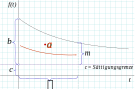
\includegraphics[width=13cm]{allg/funktionen/img/saettigung/saettigungskurveDown.png}}
\end{center}

Die Grundform eines begrenzten Zerfalls ist ein normaler
exponentieller Zerfall ($y=a^{t}$, $0<a<1$), der in $y$-Richtung um eine Sättigungsgrenze $c$ verschoben ist:

\begin{definition}{beschränkter Zerfall}{}
$$f(t) = c + b\cdot{}a^{\frac{t}{\tau}}$$
\end{definition}

Dabei ist:
\begin{itemize}
  \item $c+b = f(0) = y$-Achsenabschnitt = Startwert
	\item $c$: Die Sättigungsgrenze\index{Sättigungsgrenze} (Sättigungswert). Dies ist die Annäherungskonstante oder der \textbf{Asymtote}nwert\index{Asymptote}: Tiefer kann die Funktion nicht fallen.

	\item $m$:
    Sättigungs\textbf{differenz}\index{Sättigungsdifferenz}\index{Differenz!zur
      Sättigung}. Wie viel fehlt, bis zur
    Sättigungsgrenze: $m = f(t) - c$. Die Sättigungs\textbf{differenz} nimmt exponentiell ab.
	\item $b$: Die \textbf{Abweichung} zu $c$ zum Zeitpunkt $t=0$. Der
    Anfangswert ist somit $f(0) = c + b$; mit anderen Worten: $b$ ist das
    \textbf{Sättigungsdifferenz} zum Zeitpunkt $t_0 = 0$.

    \item $a=\frac{m}{b}=\frac{f(\tau)-c}{f(0)-c}$: Der Faktor der Veränderung der
      Sättigung\textbf{differenz}.
\end{itemize}

\subsection*{Aufgaben}
\GESOAadBMTA{359}{35. (Kuchen) und 36. (Ovomaltine)}
\olatLinkGESOKompendium{3.4.2}{33}{48. (Achtung: Das
  Kompendium verwendet andere Buchstaben: Das dortige $a$ ist unser $b$.)}

\GESO{\olatLinkArbeitsblatt{Exponentialfunktionen}{https://olat.bbw.ch/auth/RepositoryEntry/572162163/CourseNode/106029175831971}{Kap. 3.1:
    Sättigung: Begrenzter Zerfall}}
\TALS{\olatLinkArbeitsblatt{Exponentialfunktionen}{https://olat.bbw.ch/auth/RepositoryEntry/572162090/CourseNode/106029175777725}{Kap. 3.:
    Sättigung: Begrenzter Zerfall}}
\newpage


\subsection{Sättigung (begrenztes Wachstum)}\index{Sättigung}\index{begrenztes Wachstum}\index{Wachstum!begrenztes}
\subsubsection{Einstiegsbeispiel 1: Eistee wärmen}
Das Aufwärmen von Eistee von $5\degre$ Kühlschranktemperatur auf $20\degre$ Zimmertemperatur ist ein klassisches «Begrenztes Wachstum» (mit gespiegelter Exponentialfunktion).

\TNT{5.2}{Skizze}

\subsubsection{Einstiegsbeispiel 2: Batterie laden}
\begin{center}
\raisebox{-1cm}{
\includegraphics[width=8cm]{allg/funktionen/img/saettigung/batterien.png}}
\end{center}

Eine 9V-Batterie ist etwas mehr als zur Hälfte entladen und enthält nun eine
Restspannung von 4V.

Wenn wir 9V an die Batterie anlegen, so wird die Batterie geladen.

Die Batterie lädt sich umso rascher, je \textit{leerer} sie ist.

Die Batterie lädt sich umso langsamer, je \textit{voller} sie ist.


\newpage

\subsubsection{Allgemeine Form von Sättigungsprozessen}

\begin{center}
\raisebox{-1cm}{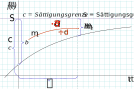
\includegraphics[width=13cm]{allg/funktionen/img/saettigung/saettigungskurve.png}}
\end{center}

Die Grundform des begrenzten Wachstums ist ein exponentieller Zerfall\totalref{zerfallsfunktion},
der an der $x$-Achse gespiegelt und in $y$-Richtung
verschoben ist:

\begin{definition}{Sättigung}{}
$$f(t) =c - b\cdot{} a^{\frac{t}{\tau}}$$
\end{definition}

Die Variable haben die folgenden Bedeutungen:

\begin{itemize}
	\item $c$: Sättigungsgrenze. Dies ist die Annäherungskonstante oder der Asymtotenwert. Höher kann die Funktion nicht steigen.

	\item $m$ ist die
    Sättigungsdifferenz\index{Sättigungsdifferenz}\index{Differenz!zur
    Sättigung}. Wie viel fehlt, bis zur
    Sättigungsgrenze: $m = c - f(t)$. Auch hier nimmt die Sättigungs\textbf{differenz} exponentiell ab.
	\item $b$: Die Abweichung des Funktionsgraphen zu $S$ zum Zeitpunkt $t=0$. Der
    Anfangswert ist somit $f(0) = c - b$.
\item $a=\frac{m}{b}=\frac{c-f(\tau)}{c-f(0)}$ Faktor der Veränderung
  der Sättigungs\textbf{differenz}.
\end{itemize}


\subsubsection{Bemerkungen}
\begin{bemerkung}{}{}
  Für die Sättigungsdifferenz gilt:

\TNT{4}{$$m = m(t) = c - f(t) = c - \left(c-b\cdot{}a^{\frac{t}{\tau}}\right) = + b\cdot{}a^{\frac{t}{\tau}}$$

und somit:

$$m_0 = m(0) = b\cdot{}a^0 = b$$}%% END TNT
\end{bemerkung}

\TRAINER{ Bemerkung (Trainer/mündlich):
  
Das $a$ kann aus zwei \textbf{beliebigen} Sättigungsdifferenz-Werten berechnet werden (die um die
Zeitdifferenz $\tau$ auseinander liegen):
$$\frac{m_2}{m_1} = \frac{b\cdot{}a^{\frac{t_2}{\tau}}}{b\cdot{}
  a^{\frac{t_1}{\tau}}} = a^{\frac{t_2}{\tau}} : a^{\frac{t_1}{\tau}} =
a^{\frac{t_2-t_1}{\tau}} = a^{\frac{\tau}{\tau}} = a$$%% 
}%% END Trainer


\begin{bemerkung}{}{}
Meistens ist $m_0$ zum Zeitpunkt $t=0$ bekannt und somit ist $b=m_0$. Es reicht, die Messung zum Zeitpunkt $t_0$ und zu einem weiteren Zeitpunkt durchzuführen. Wenn zusätzlich die Sättigungsgrenze $c$ bekannt ist, kann die Funktion $f$ komplett bestimmt werden.
\end{bemerkung} 

\newpage

\subsection{Referenzaufgaben}

\subsubsection{Berechnung am Batterie-Beispiel}\index{Batterie}
Eine Batterie weist zum Zeitpunkt $t_0$ vier Volt auf. Nach sechs Stunden am Ladegerät zeigt die Messung sieben Volt. Wir wissen, dass die Sättigungsgrenze (Ladespannung) bei neun Volt liegt.

Zeichnen Sie die gegebenen Größen in ein Koordinatensystem ein und markieren Sie bei neun Volt eine horizontale Beschränkungslinie (\zB 1V = 1 Häus'chen in $y$-Richtung; 1h = 1 Häus'chen in $x$-Richtung).

\noTRAINER{\mmPapier{8.8}}
\TRAINER{\bbwCenterGraphic{15cm}{allg/funktionen/img/saettigung/batterieFct.png}}

\textbf{Frage 1}: Wie lautet die Formel $f(t) = ...$ der Sättigungskurve?

\noTRAINER{$c = ..........................$}
\TRAINER{$c = \textrm{ Sättigungsgrenze } = 9 [\textrm{V}]$}

\noTRAINER{$b = ..........................$}
\TRAINER{$b = m_0 = c-f(0) = 9 - 4 = 5$}

\noTRAINER{$m =  ..........................$}
\TRAINER{$m = m_1 = c-f(\tau) = 9 - 7 = 2$}

\noTRAINER{$a = .........................$}
\TRAINER{$a=\frac{m}{b} = \frac{m_1}{m_0} = \frac{2}{5} = 0.4$}

\noTRAINER{$\tau = .........................$}
\TRAINER{$\tau = 6$ ($e_x$ = eine Stunde)}


\noTRAINER{$f(t) = c - b\cdot{}a^{\frac{t}{\tau}} = ..... - .....\cdot{}(.....)^{\frac{-t}{.....}}$}
\TRAINER{$f(t) = c - b\cdot{}a^{\frac{t}{\tau}} = 9 - 5\cdot{}(\frac{2}{5})^{\frac{t}{6}}$}

\TRAINER{Die Kontrollen für $t=0$ und $t=6$ sind mit dem Stehenlassen von $a$ als Bruch nun sehr einfach.}
\newpage

\textbf{Frage 2}: Wann wird die Batterie zu 99\% geladen sein?

\TNTeop{99\% von 9V = 8.91 V

  Somit ist $t$ gesucht mit $f(t) = 9 - 5\cdot{}\left(\frac25\right)^{\frac{t}{6}} = 8.91$

  (beidseitig -9 und Vorzeichen drehen und dann durch 5 teilen, so folgt...)

  $$(0.4)^{\frac{t}{6}} = (9-8.91) : 5 = 0.09 : 5 = 0.018$$

  Definition Logarithmus:

  $$\frac{t}6 = \log_{0.4}(0.018) \approx 26.3 $$

  Nach ca. 26 - 27 Stunden ist die Batterie zu 99\% geladen.
}
\newpage

\subsubsection{Referenzaufgabe Sättigung: Pneu}\index{Reifen}\index{Pneu}

Ein Reifen (Pneu) ist anfänglich ganz leer und enthält «nur» 1 atm, nämlich den
Druck der Umgebung. (1 atm = atmosphärischer Druck = technische Atmosphäre) 

Der Reifen wird aufgepumpt mit einer Druckpumpe, die maximal 2 atm
leisten
kann. Mit 2 atm ist hier gemeint: 2 at mehr als der
Umgebungsdruck. Somit könnte der Pneu bis auf maximal 3 atm aufgepumpt
werden (= Sättigungsgrenze).

Um den Reifen optimal zu füllen, wird er auf 2 atm aufgepumpt (1 atm
über dem Umgebungsluftdruck).

Die Pumpe schafft in den ersten 10 Sekunden den Druck von 1 atm auf 1.2
atm (= 0.2 atm über Normaldruck) aufzupumpen.

Nach wie vielen Sekunden muss gestoppt werden, damit der Reifen
optimal gepumpt ist?

\TNTeop{Die Sättigungsdifferenz schwindet von $m_1=3-1=2$ bis $m_2=3-1.2=1.8$
innerhalb der ersten $10s = \tau$. Die Sättigungsgrenze liegt bei
$S=3$. Unsere (Exponential)basis $a$ ist somit $1.8 / 2$, was uns
liefert:
$$f(t) = 3 - 2\cdot{}\left(\frac{1.8}{2}\right)^\frac{t}{10}$$
Somit ist das Optimum bei $2 = 3-
2\cdot{}\left(\frac{1.8}{2}\right)^\frac{t}{10}$ erreicht, also bei
etwa 65.8 Sekunden.
}
\newpage

\GESO{\subsection*{Aufgaben}}
\GESOAadBMTA{358}{34. (Eistee)}
\olatLinkGESOKompendium{3.4.2}{32ff}{49. - 51. (Bem.: Das
  Kompendium gibt die Funktionsterme bereits an und verwendet als
  Basis i.\,d.\,R. die Eulersche Konstante $e\approx{} 2.71828$)}

\GESO{\olatLinkArbeitsblatt{Exponentialfunktionen}{https://olat.bbw.ch/auth/RepositoryEntry/572162163/CourseNode/106029175831971}{Kap. 3.1:
    Begrenztes Wachstum}}%% END GESO
\TALS{\olatLinkArbeitsblatt{Exponentialfunktionen}{https://olat.bbw.ch/auth/RepositoryEntry/572162090/CourseNode/106029175777725}{Kap. 3.1:
    Begrenztes Wachstum}}%% END TALS

\newpage

\subsection{Zusammenfassung der Prozesse}
\vspace{8mm}
\begin{center}\textbf{Wachstum und Zerfall}\end{center}

\TNT{8.8}{\bbwCenterGraphic{18cm}{allg/funktionen/img/zusammenfassung_exp/wachstum_zerfall.png}

  bzw.
  $$f(t) = G_0 \cdot{} \e^{qt}; q=  \frac{\ln(a)}\tau  \,\,\,\,\,\,\,\,\, f(t) = G_0 \cdot{} \e^{-qt}; q  = \frac{-\ln(a)}\tau$$
}%% END TNT

\vspace{8mm}
\begin{center}\textbf{Sättigung}\end{center}

\TNTeop{\bbwCenterGraphic{18cm}{allg/funktionen/img/zusammenfassung_exp/saettigung.png}

    bzw.
     $$f(t) = S + (G_0-S) \cdot{} \e^{q\cdot{}t}; q=    \frac{\ln(a)}\tau     \,\,\,\,\,\,\,\,\, f(t) = S + (S - G_0) \cdot{} \e^{-q\cdot{}t}; q  = \frac{-\ln(a)}\tau$$

Hier ist Platz für das Video/die Videos zur den getanzten
Funktionen (S. OLAT/Wiki).
}%% END TNTeop

\newpage

\TALS{
  \subsection*{Aufgaben}
  \olatLinkTALSStrukturaufgabenSPF{Basiskenntnisse Funktionen Teil
    1}{5}{4., 5., 8. und 9.}
  \olatLinkTALSStrukturaufgabenSPF{Basiskenntnisse Funktionen Teil
    2}{14}{45., 47. und 49.}
}%% END TALS
\newpage


%%%%%%%%%%%%%%%%%%%
%% Logarithmen (Arithmetik und Algebra III)
%%%%%%%%%%%%%%%55
%% Funktionen II GESO Metapackage
\part{Funktionen II}\index{Funktionen!II|textbf}
\renewcommand{\bbwPartID}{FCT2}
\section{Potenzfunktionen}\index{Funktion!Potenzfunktionen}\index{Potenzfunktionen}
\sectuntertitel{Funktionen hoch drei!}

\subsection*{Lernziele}

\begin{itemize}
\item Definition Ganzzahlige Potenzfunktion
\item Graphische Darstellung
\end{itemize}
\newpage


\subsection{Einstieg}

%%%%%%%%%%%%%%%%%%%%%%%%%%%%%%%%%%%%%%%%%%%%%%%%%%%%%%%%%%%%%%%%%
\subsubsection{Beispiel: Rationale Funktion\GESO{ (optional)}}

Betrachten wir einmal die Funktion $f: y = 0.1x^3 + x^2 + 2x + 3 - x^{-1}$ \zB mit Geogebra (\texttt{www.geogebra.org}).

\bbwGraph{-10}{4}{-7}{8}{%
  \bbwFunc{0.1*\x*\x*\x + \x*\x + 2*\x + 3 -1/\x}{-8.5:-0.2}
  \bbwFunc{0.1*\x*\x*\x + \x*\x + 2*\x + 3 -1/\x}{0.1:1.5}
}%%


Polynomfunktionen und rationale Funktionen sind «\textit{weiche}» Funktionen, die jedoch \textbf{Asymptoten}\index{Asymptote} (hier bei $x=0$) aufweisen können.
Ebenso sind die Extremwerte (lokale Maxima und Minima)\TALS{ wie auch die Wendepunkte} charakteristische Stellen und oft Gegenstand der Untersuchung.
Wir beschränken uns \TALS{vorerst }auf Funktionen der Art $f: y=a\cdot{}x^z$
mit $z \in \mathbb{Z}\backslash\{0\}$\TRAINER{ $z=0$ ist eine
  Proportionalität und somit hier unspannend}.

\newpage



\subsubsection{\GESO{Beispiel}\TALS{Repetition}: Reinquadratische Funktion}\index{quadratische Funktion}\index{Funktion!quadratische}

Zeichnen Sie den Graphen der Funktion $f: y= \frac16 x^2$:

\bbwGraph{-7}{7}{-1}{6.5}{%%
  \TRAINER{
    \bbwFunc{\x*\x/6}{-6:6}
  }
}%%

\begin{definition}{Reinquadratische Funktion}{}
Die Funktion

$f: y = a\cdot{}x^2$

heißt \textbf{Parabel zweiter Ordnung} oder rein-quadratische Funktion.
\end{definition}


\TALS{
\begin{bemerkung}{}{}
Eine allgemeine quadratische Funktion besitzt auch noch einen linearen ($bx$) und einen konstanten ($c$) Anteil. Die allgemeine quadratische Funktion hat die Form

$$f: y= ax^2 + bx + c$$
\end{bemerkung}
}%% END TALS

\TALS{Beispiele zu allgemeinen quadratischen Funktionen finden sie im
  Buch \cite{marthaler21alg} ab Seite 260 insb. im Bild zu Aufg. 4 auf
  Seite 273.}%% END TALS

\newpage

\subsection{Parabel}\index{Parabel}

Zeichnen Sie $y = \frac{1}{16}x^4$ im Bereich $[-3; 3]$ indem Sie für jeden 0.5-er $x$-Wert das zugehörige $y$ berechnen:

\bbwGraph{-4}{4}{-1}{6.5}{%%
  \TRAINER{\bbwFunc{\x*\x*\x*\x/16}{-3:3}}
}%%


\begin{definition}{Parabel}{definition_parabel}
  Ist $n\in \mathbb{N}_{\ge 2}$, so wird der Graph der Potenzfunktion
  $$x\mapsto a\cdot{}x^n$$
  \textbf{Parabel} $n$-ter Ordnung genannt.
\end{definition}

\TALS{%%
\begin{bemerkung}{Potenzfunktion}{definition_potenzfunktion}
  Eine Funktion der Art
$$f: y=a\cdot{}x^r$$
  mit $r \in \mathbb{R}\backslash\{0\}$ heißt \textbf{Potenzfunktion}.
\end{bemerkung}

\begin{bemerkung}{Polynomfunktionen}{}
  Funktionen, deren Funktionsterm ein Polynom bilden werden
  \textbf{Polynomfunktionen} genannt:
  $$f: y=a_n\cdot{}x^n + a_{n-1}\cdot{}x^{n-1} + a_{n-2}\cdot{}x^{n-2} + ... + a_2\cdot{}x^2 + a_1 \cdot{} x + a_0 $$
\end{bemerkung}
%
}%% END TALS


\newpage
\subsection*{Aufgaben}
\aufgabenFarbe{Zeichnen Sie die Parabeln $$y=f(x) = x^n$$ für $n = 2$,
  $n=3$, $n=4$, $n=5$ und $n=6$ mit \texttt{geogebra.org}.
\\
Was fällt auf?}
%%\GESOAadBMTA{303ff}{1. (nur $n=3$ und $n=5$), 2. (nur $n=4$ und $n=6$)}

\TNTeop{}

\newpage

\subsubsection{Anwendung (optional)}
Boltzmannsches T-hoch-vier-Gesetz\index{Boltzmann!$T^4$-Gesetz}

\leserluft{}

Die Funktion $P(T) = \sigma\cdot\varepsilon\cdot
  A\cdot{}T^4$ beschreibt, welche Strahlungsleistung $P$ ein Körper der
  Oberfläche $A$ (in $ \text{m}^2$) bei Temperatur $T$ (in Kelvin) aussendet.

  $\sigma$ = Bolzmann Konstante = $5.6\cdot{}10^{-8}$
  
  $\varepsilon$ = Emissionswert

  \small{\texttt{(eg. https://ennologic.com/wp-content/uploads/2018/07/Ultimate-Emissivity-Table.pdf)}}

  \leserluft{}
  
  Rechenbeispiel:

\TNTeop{$T$ = 20 Grad Zimmertemperatur in Kelvin: 293.15;
  Brick (Haus) hat Emissionswert ca. 0.75; Haus Oberfläche $500 \text{m}^2$

  $$P(293.15) \approx 5.6\cdot{}10^{-8} \cdot{} 0.75 \cdot{} 500
  \cdot{} 293.15^4 \approx 155 \text{kW} $$
  Natürlich strahlt eine 20-grädige Umgebungstemperatur gleich viel
  wieder zurück, sodass keine 'Heizkosten' entstehen.

  Heizen wir das Haus nun zwei Grad wärmer, so erhalten wir:
  $$P(295.15) \approx 5.6\cdot{}10^{-8} \cdot{} 0.75 \cdot{} 500
  \cdot{} 295.15^4 \approx 159.4 \text{kW} $$

  Dies entspricht einer Differenz von 4.28 kW für nur zwei Grad wärmer
  im Haus!
  

}%% END TNT
\newpage

Zeichnen Sie des weiteren die Funktion $y = \frac{1}{9}x^3$:

\bbwGraph{-4}{4}{-5}{5}{%%
  \TRAINER{\bbwFunc{\x*\x*\x/9}{-3.5:3.5}}
}%%

\subsubsection{Symmetrien}\index{Symmetrien!von Parabeln}\index{Parabel!Symmetrie}
Was fällt für gerade und ungerade Exponenten auf? Gibt es Spiegelachsen
oder Spiegelpunkte?

\renewcommand{\mmPapier}[1]{\mmPapierZwei{#1}{16.4}}
\begin{tabular}{c|p{8cm}}
  $x^2$ & \vspace{0.1mm}\TNT{0.8}{An der $y$-Achse}\\\hline
  $x^3$ & \vspace{0.1mm}\TNT{0.8}{Am Ursprung $O(0|0)$}\\\hline
  $x^4$ & \vspace{0.1mm}\TNT{0.8}{wie $x^2$}\\\hline
  $x^5$ & \vspace{0.1mm}\TNT{0.8}{wie $x^3$}\\\hline
\end{tabular}
\renewcommand{\mmPapier}[1]{\mmPapierZwei{#1}{17.6}}


\GESO{Eine Zusammenfassung der wichtigsten Eigenschaften von
  Potenzfunktionen finden Sie im Buch \cite{marthaler21alg} Seite 296 oben.}
\newpage

\subsubsection{Referenzaufgabe}

Bestimmen Sie $a$ und $k$ so, dass der Graph von $y = a \cdot{} x^k$
durch die Punkte $P=\left(3 \middle| 1458\right)$ und
$Q=\left(-4\middle|8192\right)$ verläuft.

\TNT{15.2}{ Punkte einsetzen in die Funktionsgleichung:
  \gleichungZZ{1458}{a\cdot{}3^k}{8192}{a\cdot{}(-4)^k}
  Aus der oberen Gleichung das $a$ ermitteln ($a=\frac{1458}{3^k}$)
  (I) und in die zweite
  Gleichung einsetzen: $$8192 = \frac{1458}{3^k} \cdot{} (-4) ^k$$
  Exponent $k$ separieren:
  $$\frac{8192}{1458} = \left(\frac{-4}3\right)^k$$
  Problem: Logarithmen mit negativen Basen (hier $\frac{-4}3$)
  funktionieren nicht!
  
  Weil nun $k$ gerade sein muss, folgt dass $\left(\frac{-4}3\right)^k
  = \left(\frac43\right)^k$. Daraus ergibt sich
  $$\frac{8192}{1458} = \left(\frac{4}3\right)^k \Longrightarrow k =
  \log_{\frac43}\left(\frac{8192}{1458}\right) = 6$$
  Dieses $k$ nun in die Gleichung (I) einsetzen; dies
  liefert
  $$a=\frac{1458}{3^k} = 2.$$
}%% end TRAINER


\subsection*{Aufgaben}
\AadBMTA{305ff}{11. a) b) c), 13. a) c), (optional 17.,)  18.}
%%\TALSAadBMTA{197}{735. (6) (7) und (9) jeweils mit geogebra, 736. a) d),
%%  737. a) c), 739.}
\newpage


\subsection{Translationen}\index{Manipulation!Funktionen}\index{Funktions-Manipulation}\index{Translation!Funktion}
\sectuntertitel{Manipulation an Funktionsgraphen}
(Verschiebung\index{Verschiebung}, Spiegelung\index{Spiegelung},
Streckung\index{Streckung})

\TadBMTA{217}{13.3}
%%\TALSTadBFWA{163}{3}
Betrachten Sie die Funktionen

$$f(x) = a\cdot{}\left(\frac{x\TALS{-d}}b\right)^5\TALS{+c}$$
und
$$g(x) = a\cdot{}\left(\frac{x\TALS{-d}}b\right)^4\TALS{+c}$$

mit Geogebra (\texttt{geogebra.org})
und beschreiben Sie die Effekte der Parameter

$a$: \TRAINER{Streckung in $y$-Richtung. $a$ negativ: Spiegelung an der
$x$-Achse.}

\noTRAINER{\mmPapier{2.4}}

$b$: \TRAINER{Streckung entlang der $x$-Achse. $b$ negativ: Spiegelung
  an der $y$-Achse.}

\noTRAINER{\mmPapier{2.4}}

\TALS{%% nur TALS haben Verschiebungen
  $c$: \TRAINER{Verschiebung entlang der $y$-Achse}

\mmPapier{2.4}
}%% end TALS

\TALS{
$d$: \TRAINER{Verschiebung entlang der $x$-Achse (Verschiebung nach
  rechts verlangt ein negatives $d$.)}

\noTRAINER{  \mmPapier{2.4}}
}%% END TALS

\newpage

\subsubsection{Zusammenfassung der Translationen}


Wir betrachten die verschiedenen geometrischen
Funktions-«Manipulationen» (Abbildungen) am Beispiel {\color{red}$y =f(x) = \frac18 x^3$}.


\newcommand{\graphTranslationMultiColumn}[5]{%
  \multicolumn{3}{|l|}{#1}\\%%
\hline%%
\graphTranslationMultiColumnZ{#2}{#3}{#4}{#5}
}%% end new command \graphTranslationMultiColumn

\newcommand{\graphTranslationMultiColumnZ}[4]{%
\multirow{5}{6cm}{#1} &  & \multirow{2}{*}{\begin{minipage}{.3\textwidth}\raisebox{-8cm}{\includegraphics[width=\linewidth,height=60mm]{allg/funktionen/img/translation/#4}}\end{minipage}}\\[55mm]%%
&\fbox{#2}&\\%%
&&\\%%
&{\color{red}\fbox{#3}}&\\%%
&&\\%%
\hline%%
}%% end new command \graphTranslationMultiColumnZ

\TALS{%% Nur TALS haben Verschiebungen
\begin{tabular}{|p{7cm}|c|c|}%%
\hline%%
\graphTranslationMultiColumn{Verschiebung in $y$-Richtung...}{... um \textbf{zwei} Einheiten nach \textbf{oben}:}{$g(x)=f(x)\textbf{+2}$}{$g(x)=\frac18x^3\textbf{+2}$}{typ1.png}
\graphTranslationMultiColumnZ{... um \textbf{eine} Einheiten nach \textbf{unten}:}{$g(x)=f(x)\textbf{-1}$}{$g(x)=\frac18x^3\textbf{-1}$}{typ2.png}
\end{tabular}%%
}%% end TALS

\begin{tabular}{|p{7cm}|c|c|}%%
\hline%%
\graphTranslationMultiColumn{Spiegelung...}{... an der $x$-Achse:}{$g(x)=-f(x)$}{$g(x)=-\frac18x^3$}{typ3.png}
\graphTranslationMultiColumnZ{... an der $y$-Achse:}{$g(x)=f(-x)$}{$g(x)=\frac18(-x)^3$}{typ4.png}
\end{tabular}%%

\begin{tabular}{|p{7cm}|c|c|}%%
\hline%%
\graphTranslationMultiColumn{Streckung...}{... in $y$-Richtung (von der $x$-Achse aus) um Faktor \textbf{zwei}:}{$g(x)=\textbf{2}\cdot{}f(x)$}{$g(x)=\textbf{2}\cdot{}\frac18x^3$}{typ5.png}
\graphTranslationMultiColumnZ{... in $x$-Richtung (von der $y$-Achse aus) um Faktor \textbf{zwei}:}{$g(x)=f(\frac{1}{\textbf{2}}\cdot{}x)$}{$g(x)=\frac18(\frac{1}{\textbf{2}}\cdot{}x)^3$}{typ6.png}
\end{tabular}%%

\TALS{%% Nur TALS verschieben in x-Richtung
\begin{tabular}{|p{7cm}|c|c|}%%
\hline%%
\graphTranslationMultiColumn{Verschiebung in $x$-Richtung\footnote{Kein prüfungsrelevantes Thema.}...}{... um \textbf{zwei} Einheiten nach \textbf{links}:}{$g(x)=f(x\textbf{+2})$}{$g(x)=\frac18(x\textbf{+2})^3$}{typ7.png}
\graphTranslationMultiColumnZ{... um \textbf{zwei} Einheiten nach \textbf{rechts}:}{$g(x)=f(x\textbf{-2})$}{$g(x)=\frac18(x\textbf{-2})^3$}{typ8.png}
\end{tabular}%%
}%% END TALS
\newpage

\subsection*{Aufgaben}
\GESO{
Skizzieren Sie $-\frac{1}{2}x^3 - 1$ im Bereich $x$ = -2 bis $x$ = +2.

\bbwGraph{-4}{4}{-5}{3}{%%
  \TRAINER{%
    \bbwFunc{-0.5*\x*\x*\x-1}{-2:2}%
  }%%
}%

Vergleichen Sie die neue Funktion mit der Parabel $y=x^3$.

\TNT{5.2}{Die neue Funktion ist an der $y$-Achse gespiegelt, ist um
  50\% gestaucht ($y$-Richtung) und ist um eine Einheit nach unten
  ($x$-Richtung) verschoben worden.}
}%% END GESO

\AadBMTA{304ff}{5. a) c) d) e), 9. a) d) e)}

 
\TALS{
  \aufgabenFarbe{Zeichnen Sie mit \texttt{geogebra.org} die Funktion
    $f(x) = \frac1{10}(x^3 - 3x^2 + 3)$
    \\
    Definieren Sie anschließend die Funktion $$g(x) = a\cdot{}f((x+s)\cdot{}b)+r.$$
\\
    Entscheiden Sie, welche Veränderungen die Parameter $a$, $b$, $r$
    und $s$ bewirken.\\
    Starten Sie mit $a=1$, $b=1$, $r=0$ und $s=0$.
  }%% END Aufgabenfarbe
  \TNT{4}{
    $r$: Verschiebung nach oben\\
    $s$: Verschiebung nach links\\
    $a$: Streckung in $y$-Richtung\\
    $b$: Stauchung in $x$-Richtung
  }%% END TNT
}%% END TALS



%%  OLAT Arbeitsblatt
\GESO{\olatLinkArbeitsblatt{Positive Potenzfunktionen zuordnen}{https://olat.bbw.ch/auth/RepositoryEntry/572162163/CourseNode/104752086007823}{(alle Beispiele)}}%% END olatLinkArbeitsblatt
\TALS{\olatLinkArbeitsblatt{Positive Potenzfunktionen zuordnen}{https://olat.bbw.ch/auth/RepositoryEntry/572162090/CourseNode/105597875231723}{(alle Beispiele)}}%% END olatLinkArbeitsblatt


\olatLinkTALSStrukturaufgabenSPF{Teil 2}{15ff}{48. und 51.}
%%\TALS{\aufgabenFarbe{Strukturaufgaben SPF Teil 2: Taschenrechner: S. 15ff:  Aufg. 48. und 51.}%% END Aufgabenfarbe
%%}%% END TALS

%%\TALSAadBMTA{197 ff.}{739., 743. c), 745. c), 738.*}

\olatLinkGESOKompendium{3.3.1.}{26}{28., 29.}
\newpage



%%%%%%%%%%%%%%%%%%%%%%%%%%%%%%%%%%%%%%%%%%%%%%%%%%%%%%%%%%%%%%%%%%%%%%%%%%%%%%%%%%%
\subsection{Hyperbel}\index{Hyperbel (negative Exponenten)}

(«Hyperbel» Griechisch = «über das Ziel hinaus werfen»)


Zur Erinnerung:
\begin{multicols}{2}
\begin{itemize}
	\item $x^{-1} = \frac{1}{x}$
	\item $x^{-2} = \frac{1}{x^2}$
	\item $x^{-3} = \frac{1}{x^3}$
	\item $x^{-4} = \frac{1}{x^4}$
	\item $x^{-5} = \frac{1}{x^5}$
  \item ...
\end{itemize}
\end{multicols}

Zeichnen Sie die Funktion $f: y = x^{-1}$ im Definitinosbereich
$\DefinitionsMenge{} = [-5;5]\TRAINER{\backslash \{0\}}\noTRAINER{......}$

\bbwGraph{-6}{6}{-3}{3}{%%
  \TRAINER{\bbwFunc{1/\x}{-5:-0.3}}
  \TRAINER{\bbwFunc{1/\x}{0.3:5}}

}%%

\newpage


Zeichnen Sie zusätzlich Funktion $f: y = x^{-2}$ im Definitionsbereich $[-5;5]$:

\bbwGraph{-6}{6}{-5}{5}{%%
  % x^-2
  \TRAINER{\bbwFuncC{1/(\x * \x)}{-5:-0.447}{green}}%% 0.447 = 1/sqrt (5)
  \TRAINER{\bbwFuncC{1/(\x * \x)}{0.447:5}{green}}
  \TRAINER{\bbwLetter{2.5,0.5}{x^{-2}}{green}}
  \TRAINER{\bbwLetter{-1.5,1}{x^{-2}}{green}}

  %x^-3
%  \TRAINER{\bbwFuncC{1/(\x * \x * \x)}{-5:-0.584}{blue}}
%  \TRAINER{\bbwFuncC{1/(\x * \x * \x)}{0.584:5}{blue}}
%  \TRAINER{\bbwLetter{0.8,0.3}{x^{-3}}{blue}}
%  \TRAINER{\bbwLetter{-1.2,-3.8}{x^{-3}}{blue}}
%  \TRAINER{\bbwLetter{1.2,4.5}{x^{-3}}{blue}}

}%%

\begin{definition}{Hyperbel}{definition_hyperbel}
  Der Graph einer Potenzfunktion $$f: y=ax^z$$
  mit $z \in \{-1, -2, -3, -4, ...\}$ heißt
\textbf{Hyperbel}\index{Hyperbel} der Ordnung $z$.
\end{definition}

Der Definitionsbereich von Hyperbeln entspricht dem Definitionsbereich
des Funktionsterms. Merke: Es darf nicht durch Null geteilt werden:

$$x^{-5} = \frac{1}{x^5} \Longrightarrow \DefinitionsMenge{} = \mathbb{R} \backslash \{0\}$$


\subsection*{Aufgaben}
\AadBMTA{306ff}{19. Zeichnung mit geogebra.org, 20.
  Zeichnung mit geogebra.org}
%%\TALSAadBMTA{205}{771. a) c) d) e) g) h) j)}


\newpage

\subsubsection{Charakteristiken}
\textbf{Spiegelungen:}\\

Welche Funktionen $x$, $x^{-1}$, $x^{-2}$, $x^{-3}$ sind an welchen Achsen bzw. Punkten gespiegelt?

\renewcommand{\mmPapier}[1]{\mmPapierZwei{#1}{16.0}}
\begin{tabular}{c|p{10cm}}
  $x^{-1}$ &  \TNT{0.8}{Am Ursprung $O(0|0)$ : Punktspiegelung}\\
  \hline
  $x^{-2}$ &  \TNT{0.8}{An der $y$-Achse: Achsensymmetrie}\\
  \hline
  $x^{-3}$ &  \TNT{0.8}{Am Ursprung $O(0|0)$: Punktspiegelung}\\
  \hline
  $x^{-4}$ &  \TNT{0.8}{An der $y$-Achse: Achsensymmetrie}\\
  \hline  
\end{tabular}
\renewcommand{\mmPapier}[1]{\mmPapierZwei{#1}{17.6}}


\paragraph{Definitions- und Wertebereiche:}

Geben Sie für die obigen Funktionen an, was ihr Definitions- bzw. Wertebereich ist\footnote{Grundmenge ist $\mathbb{R}$.}:

\begin{tabular}{c|c|c}
Funktionsterm & Definitionsbereich $\DefinitionsMenge{}$& Wertebereich $\Wertebereich{}$\\ \hline
  $x^{-1}$ & \TRAINER{$\mathbb{R}\backslash\{0\}$} &  \TRAINER{$\mathbb{R}\backslash\{0\}$}\\ \hline
  $x^{-2}$ & \TRAINER{$\mathbb{R}\backslash\{0\}$} &  \TRAINER{$\mathbb{R}^{+}\backslash\{0\}$}\\ \hline
  $x^{-3}$ & \TRAINER{$\mathbb{R}\backslash\{0\}$} &  \TRAINER{$\mathbb{R}\backslash\{0\}$}\\ \hline
  $x^{-4}$ & \TRAINER{$\mathbb{R}\backslash\{0\}$} &  \TRAINER{$\mathbb{R}^{+}\backslash\{0\}$}\\ \hline
\end{tabular}


\GESO{\subsection*{Aufgaben}}
\olatLinkGESOKompendium{3.3}{26}{28. bis 31.}
\GESO{\aufgabenFarbe{Aufgabe der Nullserie 2 (zweite Nullserie): Aufg. 7 auf Seite 3}}
\GESO{\aufgabenFarbe{Maturaprüfung 2016, Aufg. 8 (Graphen zuordnen)}}

\newpage

\newpage

%%%%%%%%%%%%%%%%%%%%%%%%%%%%%%%%%%%%%%%%%%%%%%%%%%%%%%%%%%%%%%%%%%%%%%%%%%%%%%%%%%%

\subsection{Zusammenfassungen und Überblick}\index{Potenzfunktionen!Überblick}

$$y = a\cdot{}x^z$$

$z$ gerade: Gespiegelt an der $y$-Achse

$z$ ungerade: Gespiegelt am Ursprung $O=(0|0)$

Ist ${\color{ForestGreen}a>0}$\TRAINER{ (grün in der Graphik)}, so sind Graphen mit
geraden Exponenten nach oben geöffnet bzw. mit ungeraden Exponenten im
Quadranten I und III.

Ist ${\color{red}a<0}$\TRAINER{ (rot/orange in der Graphik)}, so sind Graphen mit
geraden Exponenten nach unten geöffnet bzw. mit ungeraden Exponenten
im Quadranten II und IV.


\TRAINER{%
  \includegraphics[width=8.5cm]{allg/funktionen/img/potenzfct/potenzFunktionenGerade.png}\hfill{}\includegraphics[width=8.5cm]{allg/funktionen/img/potenzfct/potenzFunktionenUngerade.png}
}%% END Trainer
\noTRAINER{%
  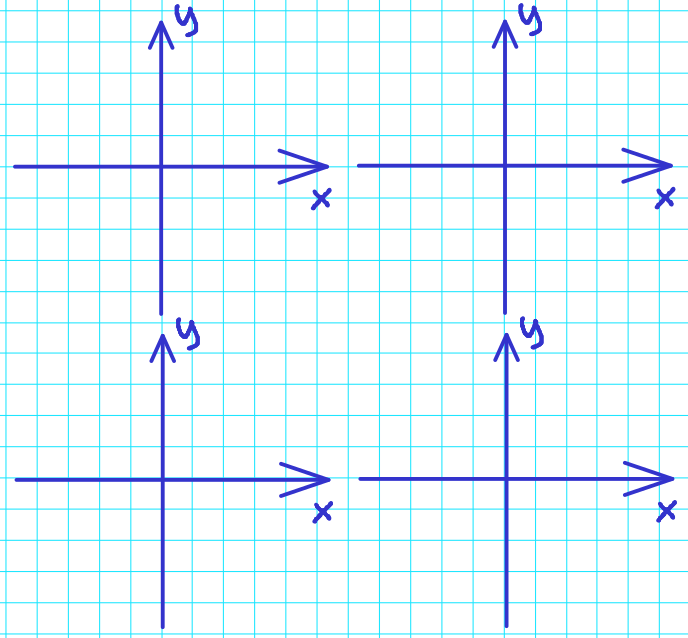
\includegraphics[width=8.5cm]{allg/funktionen/img/potenzfct/potenzFunktionenLeer.png}\hfill{}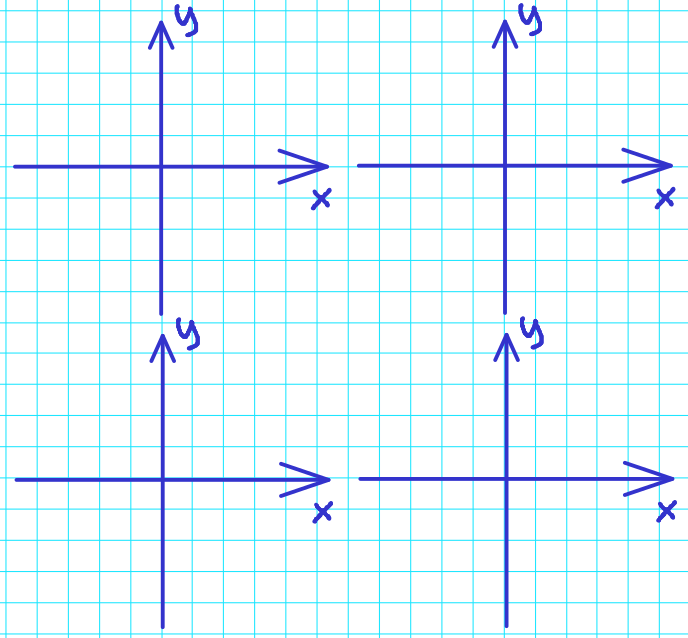
\includegraphics[width=8.5cm]{allg/funktionen/img/potenzfct/potenzFunktionenLeer.png}
}%% END Trainer


\subsection*{Aufgaben}
\AadBMTA{307}{25. b) c), 26. a)\TALS{ b)}, 27. b) c)\TALS{, 33*}}

\newpage


\newpage
\newpage
%%
%% 2019 07 04 Ph. G. Freimann
%%

\section{Exponentialfunktionen}\index{Funktion!Exponentialfunktion}\index{Exponentialfunktionen}
\sectuntertitel{Go viral!}
%%%%%%%%%%%%%%%%%%%%%%%%%%%%%%%%%%%%%%%%%%%%%%%%%%%%%%%%%%%%%%%%%%%%%%%%%%%%%%%%%
\subsection*{Lernziele}

\begin{itemize}
\item Definition Exponentialfunktion
\item Koeffizienten interpretieren
\item Graph: Symmetrien, Polstellen, Asymptoten, Schnittpunkte mit
  Achsen
  \item Basiswechsel
\end{itemize}

\TadBMTA{322}{19}
%%\TALS{(\cite{frommenwiler17alg} S.215 (Kap. 3.10))}
%%\GESO{(\cite{marthaler21alg}       S.322 (Kap. 19))}
\newpage

\subsection{Aussehen von Exponetialfunktionen}


Zeichnen Sie $f: y=2^x$ und $g: y=1.4^x$ ins selbe Koordinatensystem:


\bbwGraph{-5}{5}{-1}{5}{
\TRAINER{  \bbwFuncC{pow(2.0,\x)}{-3.5:2.1}{blue}
  \bbwFuncC{pow(1.4,\x)}{-3.5:3}{green}
  \bbwLetter{1,3}{$f$}{blue}
  \bbwLetter{2.5,2}{$g$}{green}
}%% end TRAINER
}%% end graph

\begin{definition}{Exponentialfunktion}{}\index{Exponentialfunktionen!Definition}
  Eine Funktion der Form $$f(x): x \mapsto a^x$$
  bzw. $$y = a^x$$
  mit $a\in \mathbb{R}^{+}\backslash\{1\}$ heißt \textbf{Exponentialfunktion}.
\end{definition}


\begin{bemerkung}{Zunahmefaktor}{}\index{Zunahmefaktor|textbf}
Der Parameter $a$ gibt den Wachstumsfaktor pro Zeiteinheit $e_x$ an.
\end{bemerkung}


\subsubsection*{Aufgaben}
\GESO{\olatLinkArbeitsblatt{Exponentialfunktionen}{https://olat.bms-w.ch/auth/RepositoryEntry/6029794/CourseNode/106029175831971}{Kap. 1.2:
    Einfache Wachstumsprozesse: Aufgaben 4. bis 6.}}
\TALS{\olatLinkArbeitsblatt{Exponentialfunktionen}{https://olat.bms-w.ch/auth/RepositoryEntry/6029786/CourseNode/106029175777725}{Kap. 1.2:
    Einfache Wachstumsprozesse: Aufgaben 4. bis 6.}}

\newpage

\subsection{Formen der Darstellung}
Zeichnen Sie die Funktionen $f: y=2^x$, $g: y=2^{-x}$ und $h: y=\left(\frac12\right)^x$ in dasselbe Koordinatensystem:

\bbwGraph{-6}{6}{-1}{5}{
  \TRAINER{\bbwFuncC{exp(0.69314718*\x)}{-6:2}{blue}}
  \TRAINER{\bbwFuncC{exp(-0.69314718*\x)}{-2:6}{red} }
  \TRAINER{\bbwLetter{1.5,4}{2^x}{blue}}
  \TRAINER{\bbwLetter{-5,4}{g(x)=2^{-x}=\left(\frac{1}{2}\right)^x=h(x)}{red}}
}

Bemerkung: \TRAINER{$$2^{-x} = \frac1{2^x} = \frac{1^x}{2^x}= \left(\frac12\right)^x$$}
\newpage



\subsubsection{Umkehrung (Optional)}
Um aus einem Wachstum einen Zerfall zu modellieren können wir entweder
die Zeitachse umdrehen oder den Kehrwert der Basis verwenden.
umgedreht werden:

Mit $d := \frac1a $ gilt:

\begin{center}
  \fbox{$a^{+t} = \left(\frac1a\right)^{-t} = d^{-t} $}
\end{center}

\newpage

\newpage

\subsection{Verschiebung und Streckung \GESO{(optional)}}

Eine Verschiebung der Exponentialfunktion $y=b\cdot{}a^x$ in der Zeit ($x$-Richtung) kann auch in Form einer Veränderung der Startfaktors $b$ umgeschrieben werden.

Verschieben wir \zB $$y=2^x$$ um fünf Einheiten nach rechts, so liest sich die neue Funktionsgleichung wie folgt:
$$y=2^{x-5}.$$

(Zeichnen Sie in \texttt{geogebra.org} a) $y=2^x$ und b) $y=2^{x-5}$.)

Dies kann jedoch auch umgeschrieben werden:

$$2^{x-5} = 2^x \cdot{} 2^{-5} = 2^{-5} \cdot{} 2^x = \frac{1}{2^5} \cdot{} 2^x =
\frac{1}{32}\cdot{}2^x$$

\bbwCenterGraphic{8cm}{allg/funktionen/img/exp/verschiebung_gleich_streckung.png}
Bildlegende: Eine Verschiebung ($x$-Richtung) der Exponentialfunktion entspricht einer Stauchung ($y$-Richtung) der selben Exponentialfunktion.

\TALS{Es gilt hier $$a^{x-b}=\frac{a^x}{k}$$ mit
$k=a^b$ und mit $b=\log_a(k)$.}

\newpage


\subsection{Punkte einsetzen\GESO{ (optional)}}
Wie bei den linearen Funktionen oder bei den Potenzfunktionen können auch Exponentialfunktionen gefunden werden, wenn bereits Punkte auf dem Graphen bekannt sind:

\textbf{Referenzaufgabe}

Finden Sie die Parameter $a$ und $b$ der Exponentialfunktion
$$f: y=b\cdot{}a^x$$
wenn Sie wissen, dass die Funktion durch die Punkte $P=(2|4)$ und $Q=(-1|2)$ verläuft:

\TNTeop{
  In Gleichung einsetzen:

  \gleichungZZ{4}{b\cdot{}a^2}{2}{b\cdot{}a^{-1}}

  Einsetzverfahren: Zum Beispiel aus der zweiten Gleichung das $b$ ermitteln...
  $$b = 2 a (III)$$
  ... und in die erste Gleichung einsetzen:

$$4 = 2a\cdot{} a^2$$
  $$2 = a^3$$
  $$a=\sqrt[3]{2}$$
  In (III) einsetzen:

  $$b = 2 \sqrt[3]{2}$$

  Ergo: $$f(x) = b\cdot{}a^x = 2\cdot{}\sqrt[3]{2} \cdot{} \left(\sqrt[3]2\right)^x \approx 2.5198 \cdot{} 1.2599^x$$
}

\subsection*{Aufgaben}
%%\AadBMTA{334}{10. a) b)\TALS{ e)}\GESO{ f)}}
\GESO{\olatLinkArbeitsblatt{Exponentialfunktionen}{https://olat.bms-w.ch/auth/RepositoryEntry/6029794/CourseNode/106029175831971}{Kap. 2.1: E-Funktion / Punkte-Aufgaben Aufg 26. a) b) ($e^{qt}$ optional) und Aufg. 27.}}
\TALS{\olatLinkArbeitsblatt{Exponentialfunktionen}{https://olat.bms-w.ch/auth/RepositoryEntry/6029786/CourseNode/106029175777725}{Kap. 2.1: E-Funktion / Punkte-Aufgaben Aufg 26. a) b) ($e^{qt}$ optional) und Aufg. 27.}}

\AadBMTA{336}{23. d}

\newpage

\newpage
%% 2019 07 04 Ph. G. Freimann
%%

\section{Wachstum und Zerfall}\index{Wachstum}\index{Zerfall}
\sectuntertitel{Sagt ein großer Stift zum kleinen Stift: ``Wachsmalstift!''}

%%%%%%%%%%%%%%%%%%%%%%%%%%%%%%%%%%%%%%%%%%%%%%%%%%%%%%%%%%%%%%%%%%%%%%%%%%%%%%%%%

\TRAINER{
  Video \href{https://www.youtube.com/watch?v=TMaLuks8dxw}{MatheMann}
Wo schneiden sich $x^3$ und $e^x$?}%%
\subsection*{Lernziele}

\begin{itemize}
\item Zinseszins
\item Wachstums-, Zerfallsprozesse
\item Verdoppelungs- und Halbwertszeiten
%%\item Basiswechsel
\end{itemize}

\TadBMTA{342}{20}
%%\TALS{(\cite{frommenwiler17alg} S.221 (Kap. Exponentielles Wachstum))}
%%\TALS{(\cite{frommenwiler17alg} S.223 (Kap. Exponentielle Abnahme))}
%%\TALS{(\cite{frommenwiler17alg} S.225 (Kap. Zinseszins))}
%%\GESO{(\cite{marthaler21alg}       S.342 (Kap. 20))}

\newpage


\subsection{Beispiele}
Bei Wachstumsprozessen sprechen wir dann von einer exponentiellen
Zunahme, wenn die Zunahme pro Zeiteinheit immer proportional zum aktuellen Bestand ist.

\begin{itemize}
\item \Lueckentext{Zinseszins}
\item \Lueckentext{Frequenzen in der temperierten Stimmung
  (Musik). Zunahme der Frequenz pro Halbtonschritt.}
\item \Lueckentext{Keime in der Kuhmilch; Ansteckungsbedingte Krankheitsfälle (\zB viral)}
\item \Lueckentext{Algenbefall in Teichen}
\item \Lueckentext{Generell Populationen: Flechten, Pilze}
\item \Lueckentext{(ungebremstes) Bevölkerungswachstum / bzw. Tierpopulation}
\item \Lueckentext{\dotfill}
\end{itemize}


\GESO{\olatLinkArbeitsblatt{Exponentialfunktionen}{https://olat.bms-w.ch/auth/RepositoryEntry/6029794/CourseNode/106029175831971}{Kap. 1.1:
    Voraussetzungen: Aufgaben 1. bis 3.}}
\TALS{\olatLinkArbeitsblatt{Exponentialfunktionen}{https://olat.bms-w.ch/auth/RepositoryEntry/6029786/CourseNode/106029175777725}{Kap. 1.1:
    Voraussetzungen: Aufgaben 1. bis 3.}}


\newpage

\subsection{Einstiegsbeispiel Taschengeld}

Bei Familie Cash kann man aussuchen, wie sich sein Taschengeld über
die Jahre «vermehrt». Mani wählt Variante A. Bei Varante A erhält man
CHF 1.- im ersten Jahr, CHF 2.- im 2. Jahr, CHF 3.- im 3. Jahr und so
weiter bis zur abgeschlossenen Grundbildung im 13. Jahr CHF 13.-.

Carla wählt Variante B. Bei der Variante B erhält Carla auch CHF 1.-
im ersten Jahr, dann aber jedes Jahr 30\% mehr, als im Vorjahr.

a) Wird Carla vor Ende der Grundbildung jemals mehr als Mani erhalten?

\LoesungsRaumLang{Ja, im 10. Schuljahr}

b) Wer hat über alle Jahre mehr Taschengeld?

\LoesungsRaumLang{Carla wird mehr haben}

c) Skizzieren Sie beide Varianten:

\TRAINER{\bbwCenterGraphic{13cm}{allg/funktionen/img/taschengeldAusgefuellt.png}}
\noTRAINER{\bbwCenterGraphic{16cm}{allg/funktionen/img/taschengeld.png}}

\TRAINER{Optional: Zeige mit Geogebra (\texttt{geogebra.org}) $x^2$ vs. $1.2^x$. Fazit:
  Exponentielles Wachstum überholt jegliche Potenzfunktion.}



\newpage

Zeichnen Sie $f: y=2^x$ und $g: y=1.4^x$ ins selbe Koordinatensystem:


\bbwGraph{-5}{5}{-1}{5}{
\TRAINER{  \bbwFuncC{pow(2.0,\x)}{-3.5:2.1}{blue}
  \bbwFuncC{pow(1.4,\x)}{-3.5:3}{green}
  \bbwLetter{1,3}{$f$}{blue}
  \bbwLetter{2.5,2}{$g$}{green}
}%% end TRAINER
}%% end graph

\begin{definition}{Exponentialfunktion}{}\index{Exponentialfunktionen!Definition}
  Eine Funktion der Form $$f(x): x \mapsto a^x$$
  bzw. $$y = a^x$$
  mit $a\in \mathbb{R}^{+}\backslash\{1\}$ heißt \textbf{Exponentialfunktion}.
\end{definition}


\begin{bemerkung}{Wachstumsfaktor}{}\index{Wachstumsfaktor}
Der Parameter $a$ gibt den Wachstumsfaktor pro Zeiteinheit $e_x$ an.
\end{bemerkung}


\subsubsection*{Aufgaben}
\GESO{\olatLinkArbeitsblatt{Exponentialfunktionen}{https://olat.bms-w.ch/auth/RepositoryEntry/6029794/CourseNode/106029175831971}{Kap. 1.2:
    Einfache Wachstumsprozesse: Aufgaben 4. bis 6.}}
\TALS{\olatLinkArbeitsblatt{Exponentialfunktionen}{https://olat.bms-w.ch/auth/RepositoryEntry/6029786/CourseNode/106029175777725}{Kap. 1.2:
    Einfache Wachstumsprozesse: Aufgaben 4. bis 6.}}


\newpage

\subsection{Exponentieller Zerfall}\label{zerfallsfunktion}
Die Funktion $f(x): x \mapsto y = d^{-x}$ ist eine
Exponentialfunktion, die gegen Null geht.

\bbwFunction{-4}{4}{-1}{8}{exp(-\x)}{-2:4}

\begin{bemerkung}{}{}
Oft wird bei Wachstumsprozessen die Zeitachse auch mit $t$ statt $x$ bezeichnet: $t$ steht für \textit{time}.
\end{bemerkung}

\newpage

\subsubsection{Beispiele}
\begin{itemize}
	\item \Lueckentext{Zinsliche Abschreibungen (\zB Wert eines Autos)}
	\item \Lueckentext{Radioaktiver Zerfall}
	\item \Lueckentext{Lichtintensität in Medium (Gas / Flüssigkeit / Glasfaser), dies gilt vertikal, wie auch horizontal}
	\item \Lueckentext{Atmosphärischer Luftdruck in Metern über Meer}
  \item \Lueckentext{Entladen einer Batterie bzw. eines Kondensators}
  \item \Lueckentext{Sauerstoffkonzentration in Seen (\zB Herbst bei kontinuierlicher Abnahme)}
  \item \Lueckentext{Abnahme des Bierschaums im Glas}
  \item \Lueckentext{Mischen, wie im Sirup-Beispiel\totalref{sirup_beispiel}}
  \item \Lueckentext{«Halbwertszeit des Wissens» ;-)}
  \item \Lueckentext{\dotfill}
\end{itemize}

\newpage



Zeichnen Sie die Funktionen $f: y=2^x$, $g: y=2^{-x}$ und $h: y=\left(\frac12\right)^x$ in dasselbe Koordinatensystem:

\bbwGraph{-6}{6}{-1}{5}{
  \TRAINER{\bbwFuncC{exp(0.69314718*\x)}{-6:2}{blue}}
  \TRAINER{\bbwFuncC{exp(-0.69314718*\x)}{-2:6}{red} }
  \TRAINER{\bbwLetter{1.5,4}{2^x}{blue}}
  \TRAINER{\bbwLetter{-5,4}{g(x)=2^{-x}=\left(\frac{1}{2}\right)^x=h(x)}{red}}
}

Bemerkung: \TRAINER{$$2^{-x} = \frac1{2^x} = \frac{1^x}{2^x}= \left(\frac12\right)^x$$}
\newpage

\subsubsection{Grundform} \index{Exponentieller Prozess! Grundform}
Die Grundform für Zerfallsprozesse lautet:

\begin{definition}{Zerfall}{}\index{Zerfall}
  Die Grundform des exponentiellen Zerfalls wird beschrieben durch die Funktion
$$f(x): x \mapsto a^x$$
  bzw.
  $$y = a^x$$
\end{definition}


\begin{gesetz}{Wachstum vs. Zerfall}{}

  Der einzige Unterschied bei Wachstums- bzw Zerfallsprozessen ist der
  Faktor $a$:

  \begin{itemize}
    \item \LoesungsRaumLen{40mm}{$a>1$: Wachstum}\vspace{3mm}
    \item \LoesungsRaumLen{40mm}{$0<a<1$: Zerfall}
  \end{itemize}
  
\end{gesetz}

\begin{bemerkung}{$x$-Richtung}{}
  Exponentielle Prozesse laufen meist in der Zeit ab. Somit wird
  die $x$-Achse zur Zeitachse und meist mit $t$ (Time) bezeichnet:
  $$f(t) = a^t$$
  \end{bemerkung}


\subsubsection{Umkehrung (Optional)}
Um aus einem Wachstum einen Zerfall zu modellieren können wir entweder
die Zeitachse umdrehen oder den Kehrwert der Basis verwenden.
umgedreht werden:

Mit $d := \frac1a $ gilt:

\begin{center}
  \fbox{$a^{+t} = \left(\frac1a\right)^{-t} = d^{-t} $}
\end{center}

\newpage

\subsection*{Aufgaben}
%%\TALSAadBMTA{223ff}{840., 841., 843., 844. und 846.}

\GESO{\olatLinkArbeitsblatt{Exponentialfunktionen}{https://olat.bms-w.ch/auth/RepositoryEntry/6029794/CourseNode/106029175831971}{Kap. 1.3: Zerfall: Aufg. 7., 8. und 9.}}
\TALS{\olatLinkArbeitsblatt{Exponentialfunktionen}{https://olat.bms-w.ch/auth/RepositoryEntry/6029786/CourseNode/106029175777725}{Kap. 1.3: Zerfall: Aufg. 7. 8. und 9.}}

\AadBMTA{354}{9. (Bauchspeicheldrüse)}
\olatLinkGESOKompendium{3.4.1}{27ff}{33., 35., 36., 39. und 41.}

\newpage
%% Sirup-Beispiel
\subsection{Mischtank}\index{Mischtank}\index{Sirup}\label{sirup_beispiel}
Wird ein Glas Wasser in ein Glas Sirup geschüttet, so

\TRAINER{\bbwCenterGraphic{5cm}{allg/alg/potenzen_wurzeln/img/Schwapp.png}}%%
\noTRAINER{\bbwCenterGraphic{5cm}{allg/alg/potenzen_wurzeln/img/SchwappOhneFormel.png}}

geschieht erst mal etwas eher klebriges:
\begin{itemize}
  \item Das Wasser verdrängt den Sirup und
  \item das Sirupglas schwappt über.
\end{itemize}

Wenn man nun gleichzeitig im Sirupglas
umrührt, so mischt sich das Wasser mit dem Sirup und je länger man
Wasser einschüttet, umso verdünnter wird der Sirup.


Wie viel Sirup bleibt im Glas?

\TNT{2.4}{
Am Ende bleibt ein
Verhältnis von Wasser : Sirup = $\left(1-\frac{1}{e}\right) : \left(\frac{1}{e}\right)$
\vspace{1.5cm}
}

Diese Konstante wird oft in großen chemischen Mischtanks verwendet,
gibt aber auch ein Maß an, wenn \zB in einer Minergie-Wohnung die Luft
ausgetauscht wird. Wenn nämlich das Volumen der Wohnung einmal neu hineingepumpt (bzw. weggeblasen) wurde während sich alte die Luft im Haus permanent mit der neuen vermischt, so ist noch ein Anteil von \TRAINER{$\frac{1}{e}$}\noTRAINER{ ..... } der alten Luft im Haus.
\newpage


\textbf{Begründung:}\\
1. Gedanke: Jedes eingefüllte Glas, vermindert die vorhandene
Sirupkonzentration um den selben Faktor. Ergo handelt es sich um
einen exponentiellen Zerfall.

\leserluft

2. Gedanke: Wir tauschen drei Mal $\frac13$ aus. Nehmen also im
\begin{itemize}
\item \textbf{ersten Schritt} $\frac13$ des Sirups weg (und ersetzen diesen mit Wasser).
  Es bleiben $\frac23$ Sirup. Den Rest füllen wir mit Wasser auf.
\item Im \textbf{zweiten Schritt} nehmen wir $\frac13$ des Gemisches
weg; es verbleiben also $\frac23$ von $\frac23$ an
Sirup-Konzentrat. Der Rest wird immer wieder mit Wasser aufgefüllt. Mit
anderen Worten: Es bleiben $\frac23 \cdot \frac23
= \left(\frac23\right)^2$ an Sirup\footnote{Man könnte hier auch argumentieren mit: «Wir nehmen von den $\frac23$ einen Drittel weg»: $\frac23 - (\frac13$ von $\frac23)$ = $\frac23 - (\frac13 \cdot\frac23) = \frac23 \cdot(1-\frac13)=\frac23\cdot\frac23$}.
\item Im \textbf{dritten Schritt} entnehmen wir wieder $\frac13$ des
Gemisches; es verbleiben wieder $\frac23$ vom bisherigen Sirup, also
$\frac23$ von $(\frac23)^2$ also $\left(\frac23\right)^3$.

Beim dreistufigen Gedankenexperiment verbleiben
$\left(\frac23\right)^3 = \left(1-\frac13\right)^3$ der ursprünglichen Konzentration.
\end{itemize}
\leserluft

3. Gedanke: Das Experiment vom vorherigen Gedanken können wir natürlich auch mit immer kleineren\TALS{, sogenannten infinitesimalen,} Schritten durchführen.
Mit Centilitern \zB im dl-Glas ersetzen wir 10 Mal je $\frac1{10}$. 
So verbleibt am Schluss $\left(1-\frac{1}{10}\right)^{10}\approx 0.35$ Sirup.

\GESO{Wenn wir (\zB mit dem Taschenrechner) die Schrittanzahl immer weiter vergrößern (und somit die pro Schritt ausgetauschte Menge immer verkleinern), so ergibt sich für 1000 Schritte ein Verhältnis von $\left(1-\frac{1}{1000}\right)^{1000}\approx 0.3677 \approx \frac1{\e}$. }
\TALS{Wenn wir die Schritte permanent erhöhen (und gegen Unendlich gehen lassen), so erhalten wir den Grenzwert (lat. Limes) von

$$\lim_{n\rightarrow\infty} \left(1-\frac{1}{n}\right)^n = \frac1{\e}$$
}
\newpage

\textbf{Aufgabe 1: Sirup}\\
Wie viel Wasser muss eingeschüttet werden, damit das auf der Flasche
angegebene Verhältnis von 1:6 (1 Teil Sirup, 6 Teile Wasser) zustande
kommt?

\TNT{8}{
Bei 1x Schütten, erhalten wir $\left(\frac{1}{\e}\right)^1$ Anteil Sirup.

Bei 2x Schütten, erhalten wir $\left(\frac{1}{\e}\right)^2$ Anteil Sirup.

Somit erhalten wir den Siebtel (1:6 = $\frac17$-Anteil) indem wir die
folgende Exponentialgleichung lösen:

$$\frac17 = \left(\frac{1}{\e}\right)^n$$
Diese Gleichung lösen wir, indem wir beidseitig logarithmieren und so
erhalten wir den einzuschüttenden Teil $$n=\ln(7)\approx{1.946}.$$
}%% END TNT

\textbf{Aufgabe 2: Minerige-Haus}\\
Wenn wir also wissen wollen, wie viel Luft in ein Minergiehaus
eingepumpt werden muss, damit nur noch 1 Promille der alten Luft
vorhanden ist, so erhalten wir
\TNTeop{
  $$\text{Volumen Neuluft} = \text{Wohnungsvolumen}\cdot{}\ln(1000)$$
  $$\ln(10000) \approx 6.9$$
} %% end TNT


\newpage

\newpage


\subsection{Startwert}\index{Startwerte!bei Wachstums- und Zerfallsprozessen}

Die bisher betrachteten Exponentialfunktionen haben für den Wert $x=0$ (bzw. $t=0$) immer den
$y$-Wert = 1 bzw. 100\%.
Da in der Praxis meist konkrete Werte vorgegeben sind verwenden wir
eine \textbf{allgemeinere Form der Exponentialfunktion}.

\subsubsection{Einstiegsbeispiel}

\begin{beispiel}{Pilz}{}
  Ein Pilzbefall an einer Wand nehme täglich um 23\% der Fläche
  zu\footnote{Je nach Organismus ist auch ein quadratisches Wachstum
  vorhanden, doch für unser Experiment verwenden wir exponentielles Wachstum.}.
  Anfänglich wird eine Fläche von $35$ $\text{cm}^2$ gemessen.
  Welche Fläche ist nach einem, nach zwei, nach fünf, nach zehn
  bzw. nach $n$ 
  Tagen zu erwarten?

  \TNT{6}{Ein  Tag:   $35\cdot{} 1.23^1    =          43.05 \text{cm}^2$\\
          Zwei Tage:  $35\cdot{} 1.23^2   \approx{}  52.95 \text{cm}^2$\\
          Fünf Tage:  $35\cdot{} 1.23^5   \approx{}  98.54 \text{cm}^2$\\
          Zehn Tage:  $35\cdot{} 1.23^{10} \approx{} 277.4 \text{cm}^2$\\
          $n$  Tage:  $35\cdot{} 1.23^n = 35\cdot{}1.23^n$}%% END TNT

  Wann wird die ganze Wand ($6 \text{ m}^2$) mit dem Pilz befallen
  sein?
  
\TNT{6}{$6 \text{ m}^2 = 60\,000 \text{ cm}^2$
     
     ergo: $60\,000 = 35 \cdot{} 1.23^n$

     (durch 35 teilen, dann logarithmieren)

     $$\frac{60\,000}{35} = 1.23^n$$

     $$n = \log_{1.23}\left(\frac{60\,000}{35}\right) \approx 35.97 \text{Tage}$$

   }%% END TNT

\end{beispiel}

\newpage


\begin{gesetz}{Exponentialfunktion mit frei wählbarem Startwert}{}
$$f: y = \LoesungsRaumLen{40mm}{b\cdot{}a^x}$$

Auch hier gibt der Parameter $a$ den Wachstumsfaktor pro Zeiteinheit $e_x$ an.

Dabei ist $b$ der Startwert zum Zeitpunkt $x$ = 0.
\end{gesetz}


\noTRAINER{\bbwCenterGraphic{8cm}{allg/funktionen/img/exp/b_faktor.png}}
\TRAINER{\bbwCenterGraphic{8cm}{allg/funktionen/img/exp/b_faktor_trainer.png}}

\begin{bemerkung}{Wachstumsfaktor}{}{}
Werden zwei $x$ Positionen mit Differenz 1 (=$e_x$) betrachtet, so sind
die zugehörige $y$-Werte um \textbf{Faktor} $a$ auseinander.
\end{bemerkung}

Begründung:
\TNTeop{
  Gegeben $x_1$ und $x_2 = x_1 + 1$. So ist

  $y_1 = b\cdot{}a^{x_1}$ und $y_2 = b\cdot{}a^{x_2}$.

  Setzen wir nun $x_1 + 1$ für $x_2$ ein, so erhalten wir:

  $$y_2 = f(x_2) = b\cdot{}a^{x_2} = b\cdot{} a^{x_1+1} =  b\cdot{}a^{x_1} \cdot{} a^1 = y_1\cdotp{} a$$
}
\newpage


\subsection*{Aufgaben}

\GESO{\olatLinkArbeitsblatt{Exponentialfunktionen}{https://olat.bms-w.ch/auth/RepositoryEntry/6029794/CourseNode/106029175831971}{Kap. 1.4:
    Frei wählbarer Startwert: Aufg. 10. Gummiball; 11. Neophytenplage;
    12: Tierpopulation; 13. Licht im Wasser;  weitere Aufgaben 14. bis 17.}}
\TALS{\olatLinkArbeitsblatt{Exponentialfunktionen}{https://olat.bms-w.ch/auth/RepositoryEntry/6029786/CourseNode/106029175777725}{Kap. 1.4:
    Frei wählbarer Startwert: Aufg. 10. Gummiball; 13. Licht im Wasser. 14. Federpendel; 15. Luftdruck; weitere Aufgaben aus
    Kap. 1.4.}}
 
  \AadBMTA{338}{29. (Bierschaum)}
  \AadBMTA{353}{6. (C-14 Methode)}

  Als Vorbereitung zur allgemeinen Wachstumsfunktion:
  \AadBMTA{207}{10. (Algen)}

\newpage


\subsection{Beobachtungszeitspanne}
\subsubsection{Einstgiesbeispiel}
\bbwCenterGraphic{17cm}{allg/funktionen/img/tuerlersee2.jpg}
\begin{center}{\small Legende: Türlersee April 2022}\end{center}

Der Türlersee ist ein kleiner See im Reppischtal. Seine Oberfläche
begann sich vor einigen Jahrzehnten stark mit Algen\footnote{Genau
  genommen handelte es sich um Zooplanktonbiomasse zwischen 1982 und 1994, doch als
  Idee zur Exponentialfunktion sollte ein ungefähres Flächenmodell reichen.} zu bedecken.

Anfänglich (zum Zeitpunkt $t=0$) waren gerade mal 20$m^2$ bedeckt. Doch nach fünf Tagen hatte sich diese Fläche verdoppelt und nach weiteren fünf Tagen nochmals verdoppelt (also insgesamt vervierfacht).

Füllen Sie die (prognostizierte) Wertetabelle für 30 Tage ein:

\def\spaceX{\,\,\,\,\,\,\,\,\,\,}
\newcommand\tuerlerB[1]{\noTRAINER{\spaceX}\TRAINER{#1}}
\begin{tabular}{l|c|c|c|c|c|c|c}
  $t$:  & 0 & 5 & 10 & 15 & 20 & 25 & 30 \\
  \hline
  $m^2$ & \tuerlerB{20}  & \tuerlerB{40}  &   \tuerlerB{80}  &  \tuerlerB{160}  &  \tuerlerB{320}  &  \tuerlerB{640}  &  \tuerlerB{1280} \\
\end{tabular}

\newpage
Zeichnen Sie die Algenpopulation als Graph in eine Koordinatensystem
(beginnen Sie mit dem Ursprung ganz links unten. $x$-Achse in Tagen ($t$). $y$-Achse in $\text{m}^2$.

\noTRAINER{\bbwCenterGraphic{170mm}{allg/funktionen/img/exp/WachstumTuerlerseeLeer.png}}
\TRAINER{\bbwCenterGraphic{10cm}{allg/funktionen/img/exp/tuerlerAlgen.png}}
\newpage

\textbf{Funktionsgleichung}

Wir betrachten die selbe Algenpopulation mit einer
Ver\textbf{\color{blue}dopplung} der Fläche alle \textbf{\color{red}fünf} Tage bei einer
Startfläche von \textbf{\color{green}zwanzig} $\text{m}^2$.

Geben Sie eine Funktionsgleichung an, welche das Wachstum der
Algenpopulation beschreibt...



\begin{bbwFillInTabular}{c|c|c||c|c|c|c|c|c|c|c}\hline
  Tage      & $t$ & \cellcolor{gray!75}\noTRAINER{\hspace{2cm}} & 0            & \tiny{1-4} & 5            & \tiny{6-9} & 10           & \tiny{11-14} & 15           &\\\hline
  Fläche     & $A$ & \TRAINER{$20\cdot v$}    &
  \TRAINER{20}\noTRAINER{\hspace{15mm}} &  \cellcolor{gray!75}    &
  \TRAINER{40}\noTRAINER{\hspace{15mm}} &    \cellcolor{gray!75}  &
  \TRAINER{80}\noTRAINER{\hspace{15mm}} &         \cellcolor{gray!75}       &
  \TRAINER{160}\noTRAINER{\hspace{15mm}} &\\\hline
  Faktor    & $v$ & \TRAINER{$v=2^z$}    & \TRAINER{1}  &  \cellcolor{gray!75}    & \TRAINER{2}  &   \cellcolor{gray!75}   & \TRAINER{4}  &    \cellcolor{gray!75}            & \TRAINER{8} &\\\hline
  Intervalle & $z$ & \TRAINER{$z=\frac{t}{5}$}    & \TRAINER{0}  &  \cellcolor{gray!75}    & \TRAINER{1.}  & \cellcolor{gray!75}     & \TRAINER{2.}  &   \cellcolor{gray!75}             & \TRAINER{3.} &\\\hline
  Potenz     &\TRAINER{$2^z$} & \TRAINER{$2^\frac{t}{5}$}     & \TRAINER{$2^0$}  &   \cellcolor{gray!75}   & \TRAINER{$2^1$}  &   \cellcolor{gray!75}   & \TRAINER{$2^2$}  &  \cellcolor{gray!75}              & \TRAINER{$2^3$} &\\\hline
\end{bbwFillInTabular}

\TRAINER{Falls nicht mit Tabelle: 1. Tipp $f(0)=20; f(5)=40;
  f(10)=80;...$, dann 2. Tipp $f_B(0) = 20; f_B(1)=40; ...$ $B$=Anzahl
  Beobachtungsintervalle}

\leserluft
\begin{center}
  $f(t):\,\,\, y=\LoesungsRaumLang{{\color{green}20}\cdot{} {\color{blue}2} ^{\frac{t}{\color{red}5}}}$
  \end{center}
\TNT{4}{
Dabei bezeichnet\\20 den Startwert,\\2 den Zunahmefaktor und \\5 die Beobachtungszeitspanne.}%%

Merke:
\TNTeop{Ich muss für $t$ fünf Tage einsetzen, um auf eine Verdopplung
  zu kommen.

  Setze ich $t=0$ ein, so erhalte ich den Startwert zwanzig m$^2$.
}
%%%%%%%%%%%%%%%%%%%%%%%%%%%%%%%%%%%%%%%%%%%%%%%%%%%%%%%%%%%%%%%%%%%%%%%%%%%%%%%%%%%%%%%%%%%%%%%%%%%%

\subsubsection{Exponentieller Prozess (allgemein)}\index{Exponentieller Prozess! allgemeine Form}

\begin{gesetz}{Wachstumsprozess}{}
  Die Funktion

  $$y = f(t) = \LoesungsRaumLen{40mm}{b\cdot{}a^{\frac{t}{\tau}}}$$
  
  beschreibt einen allgemeinen exponentiellen Wachstumsprozess mit
  $$   a=\LoesungsRaumLen{50mm}{\text{Wachstumsfaktor während } \tau \text{ Tagen} }$$
  $$   b=\LoesungsRaumLen{50mm}{\text{Startwert}}$$
  $$\tau=\LoesungsRaumLen{50mm}{\text{Beobachtungszeitspanne}}$$
\end{gesetz}

Alternativ «die harte Tour» (ohne das $\tau$ mit anderer Basis):

\TNTeop{


  $$f(t) = b\cdot{}A^t$$

  $A$ = Faktor pro Tag, $t$ = Anzahl Tage, Startwert $b=f(0)$
  
  Bsp.: Die Algenzahl verdoppelt sich alle fünf Tage:

  $$f(5)        = 2 \cdot{} f(0)$$
  $$b\cdot{}A^5 = 2 \cdot{} b $$

  $$A^5 = 2$$

  $$A = \sqrt[5]{2} = 2^{\frac15} \approx 1.1487$$

  Einsetzen in $f(t) = b\cdot{} A^t$

  $$f(t) = b\cdot{} \left(\sqrt[5]{2}\right)^t  = b\cdot{}
  \left(2^{\frac15}\right)^t=b\cdot{} 2^{\frac{t}5} \approx b\cdot{} 1.1487^t$$

}%% end TNTeop


\newpage

\subsubsection{Graphische Erläuterung (optional)}


\begin{tabular}{cc}%%
  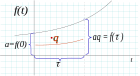
\includegraphics[width=9cm]{allg/funktionen/img/exp/exponentielles_wachstum.png} &
  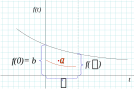
\includegraphics[width=7cm]{allg/funktionen/img/exp/exponentieller_zerfall.png}\\
\end{tabular}

%%\bbwCenterGraphic{10cm}{allg/funktionen/img/exp/exponentieller_zerfall.png}
%%\bbwCenterGraphic{11cm}{allg/funktionen/img/exp/exponentielles_wachstum.png}

Dabei sind
\begin{itemize}
\item $b=f(0)$ der Anfangsbestand zum Zeitpunkt $t$ = 0.
\item $\tau$ ist die typische Zeitspanne zwischen zwei Beobachtungszeitpunkten (zum Beispiel zwischen Wert und dessen Verdopplung). Beispiele:
  \begin{itemize}
  \item Verdoppeln in 3 Stunden: $a=2$ und $\tau = 3\, \text{h}$
    ($\text{h}$ = Stunden)
  \item Verfünf"|fachen einer Viertelstunde (= 15 Minuten): $a=5$ und
    $\tau=\frac{1}{4}\, \text{h}$
  \end{itemize}
  Meist ist die Beobachtungszeit gleichzeitig die Maßeinheit (\zB
  Veränderung pro Stunde). Dann ist unser $\tau=1$ und die Formel
  vereinfacht sich zu $f(t) = b\cdot{}a^t$.
\item $a$ ist der Zunahmefaktor zwischen zwei Beobachtungszeitpunkten (Beispiel $a=2$ bei Verdoppelungsprozessen).
  $a$ berechnet sich durch den Quotienten zwischen zwei
  Beobachtungswerten $a = \frac{f(\tau)}{f(0)} =\frac{m}{b}$.
\item
  Dabei ist $m$ der Messwert zum Zeitpunkt $\tau$.
\item $f(t)=b\cdot{}a^{\frac{t}{\tau}}$ ist der Wert (Anzahl, Fläche,
  Bestand, ...) zum Zeitpunkt
  $t$. 
\end{itemize}

Bemerkung: 
\TNTeop{
$\frac{m}b = \frac{f(\tau)}{f(0)}=\frac{b\cdot{}a^{\frac{\tau}{\tau}}}{b\cdot{}a^{\frac0{\tau}}}
  = \frac{a^1}{a^0} = \frac{a}{1} 
  = a$}%% END TNT
\newpage

\subsection{Referenzaufgabe}\index{Irland!Bevölkerungswachstum}
Irland hatte 1990 3.51 Mio. Einwohner. Im Jahr 2019 waren es bereits 4.93 Mio.

\textbf{Frage 1}: Was prognostizieren Sie für das Jahr 2025, wenn Sie von einem exponentiellen Wachstum ausgehen?

\noTRAINER{\bbwCenterGraphic{12cm}{allg/funktionen/img/exp/IrlandLeer.png}}%%

\TNTeop{
  Skizze:
  \bbwCenterGraphic{12cm}{allg/funktionen/img/exp/IrlandVoll.png}

  $\tau$ = 29 Jahre, Einheit = Jahre ($t$ in Jahren gemessen).
  
  $b=f(0) = 3.51$ [Mio EW] = Startwert (Taschenrechner STO).

  $m=f(\tau) = 4.93$ [Mio EW] = Messwert nach $\tau$ Jahren.

  $a=\frac{m}{b}=\frac{4.93}{3.51} \approx 1.4046$ pro 29 Jahre (Taschenrechner! STO). 

  $$f(t) = b\cdot{}a^\frac{t}{\tau}=b\cdot{}a^\frac{t}{29}$$


  TR Probe $b\cdot{}a^\frac{0}{29} = ? = 3.51$ 

  TR Probe $b\cdot{}a^\frac{29}{29} = ? = 4.93$ 

  Jahr 2025: $t=35$:

    $$f(35) = b\cdot{}a^\frac{35}{29}\approx 5.28899$$

}%% END TNT
\newpage

\subsection*{Aufgaben}

\GESO{\olatLinkArbeitsblatt{Exponentialfunktionen}{https://olat.bms-w.ch/auth/RepositoryEntry/6029794/CourseNode/106029175831971}{Kap. 1.5: Aufg. 18. a) b)}}
\TALS{\olatLinkArbeitsblatt{Exponentialfunktionen}{https://olat.bms-w.ch/auth/RepositoryEntry/6029786/CourseNode/106029175777725}{Kap. 1.5:     Aufg. 18. a) b) }}

\newpage

\textbf{Frage 2}: In wie vielen Jahren hat sich die Bevölkerung verdreifacht?

\TNTeop{
  Gesucht $T_3$ = Verdreifachungszeitpunkt.

  $$f(T_3) = 3\cdot{}f(0)$$

  Funktionsgleichung einsetzen:

  $$b\cdot{}a^\frac{T_3}{\tau} = 3\cdot{} b\cdot{} a^\frac0\tau$$

  Weil $a^{\frac{0}{\tau}} = 1$ folgt:

  $$b\cdot{}a^\frac{T_3}{\tau} = 3\cdot{} b$$

  $$a^\frac{T_3}{\tau} = 3$$

  Def. Logarithmus:

  $$\frac{T_3}{\tau} = \log_a(3)$$

$$T_3 = \tau\cdot{}\log_a(3) = 29\cdot{}\log_a(3) \approx 93.8$$
Die Bevölkerung wird sich voraussichtlich alle 94 Jahren
verdreifachen.

}%% END Trainer
\newpage

\subsection*{Aufgaben}
%%\TALSAadBMTA{221ff}{831 - 839}


\GESO{\olatLinkArbeitsblatt{Exponentialfunktionen}{https://olat.bms-w.ch/auth/RepositoryEntry/6029794/CourseNode/106029175831971}{Kap. 1.5:
    Aufg. 18. c), 19. - 21.}}
\TALS{\olatLinkArbeitsblatt{Exponentialfunktionen}{https://olat.bms-w.ch/auth/RepositoryEntry/6029786/CourseNode/106029175777725}{Kap. 1.5:
    Aufg. 18. c), 19. - 21. }}

\AadBMTA{338}{28. Bakterien}
\AadBMTA{352ff}{2. (Hasenpopulation), 7., 1. (optional)}
\olatLinkGESOKompendium{3.4}{27ff}{32., 34., 38., 40., 44., 45. und 46.}
\GESO{\aufgabenFarbe{Nullserie 2: Aufgabe 8.}}
\GESO{\aufgabenFarbe{Maturaprüfung 2017, Aufg. 12 (Raupen)\\
Maturaprüfung 2018 (Serie 3), Aufg. 11 (Müll)
}}



%% TODO Arbeitsblatt verlinken
%%\GESO{\olatLinkArbeitsblatt{Exponentialfunktionen}{https://olat.bms-w.ch/auth/RepositoryEntry/6029794/CourseNode/106029175831971}{Kap. 1.1: Voraussetzungen}}
%%\TALS{\olatLinkArbeitsblatt{Exponentialfunktionen}{https://olat.bms-w.ch/auth/RepositoryEntry/6029786/CourseNode/106029175777725}{Kap. 1.1: Voraussetzungen}}



\newpage

\subsection{Rate vs. Faktor
  II}\index{Rate}\index{Fatkor}\index{Zunahmefaktor}\index{Zunahmerate}
\totalref{RateZins1}

Den Unterschied von Zinsfuß (= Rate) und Zinsfaktor kennen wir bereits aus der Zinsrechnung.

So entspricht eine Zunahme von 12\% einem\\
Aufzinsungsfaktor von \LoesungsRaumLang{1.12}.

Wenn jedoch eine Beobachtung einer Zunahme von, sagen wir, 70\% innerhalb einer Viertelstunde beobachtet wird, so können wir uns fragen, um wie viel die Zunahme (als Rate oder Faktor) pro Zeiteinheit (hier Stunden) ist.


Füllen Sie dazu folgende Tabelle aus. Dabei bedeuten

\begin{tabular}{lp{14cm}}\hline
  Einheit & Stunden, Minuten, Meter, ... \\\hline
  $\tau$  & In dieser Zeitspanne (Stunden, Meter, ...) wird beobachtet \\\hline
  $p$     & Zunahme\textbf{rate}\index{Zunahmerate}\index{Rate} während $\tau$ Einheiten in \%. Ist $p$ negativ, handelt es sich um eine Abnahme\\\hline
  $a_\tau$ & Zunahme\textbf{faktor}\index{Zunahmefaktor} während $\tau$ Einheiten. Ist $a<1$, handelt es sich um einen Abnahmefaktor\\\hline
  $a_E$ (Formel)   & Zunahme pro Einheit (als Faktor). Aufgeschrieben als Formel\\\hline
  $\approx a_E$ (Zahl)  & Zunahme pro Einheit (als Näherungswert).\\\hline
  $p_E$   & Prozentuale Zunahme pro Zeiteinheit\\\hline
  \end{tabular} 

\leserluft{}
\leserluft{}
%% temporäres Platzhalterchen 
\newcommand{\ph}[1]{\noTRAINER{...........}\TRAINER{#1}}

%%\renewcommand{\arraystretch}{1.7}
$$f(t) = a_\tau^{\frac{t}\tau} = a_E^t$$
%% probably turn off auto-fill-mode in emacs when editing long lines
\begin{bbwFillInTabular}{|l|l|l|l|l|l|l|}\hline
  Einheit & $\tau$            &  $p$         & $a_\tau$         & $a_E$ (Formel)           &  $\approx a_E$    &$p_E$            \\\hline\hline
  h       &  $3$              &  56\%        & $1.56$           & $1.56^\frac13$            &  1.1598           & 11.598\%        \\\hline 
  h       &  $\frac14 = 0.25$ &  70\%        & \ph{1.7}         & \ph{ $1.7^\frac1{0.25}$}  &  \ph{8.3521}      & \ph{735.21\%}   \\\hline 
  h       &  $\frac12$        &  \ph{50\%}   & 1.5              &  $1.5^\frac1{0.5}$        &  2.25             & \ph{125\%}      \\\hline 
  Tage    &  $5$              & 100\%        & \ph{2}           & \ph{$2^\frac1{5}$}        &  \ph{1.1487}      & \ph{14.87}\%    \\\hline 
  Min.    &  $2$              & \ph{-60}\%   & 0.4              & \ph{$0.4^\frac1{2}$}      &  \ph{0.6325}      & \ph{-36.75}\%   \\\hline 
  m       &  $12$             & \ph{4.5}\%   & \ph{1.045}       & $1.045^\frac1{12}$        &  \ph{1.00367}     & \ph{0.3675}\%   \\\hline
  Wochen  & \ph{$2$}          & \ph{$200$}\% & \ph{3}           & $3^\frac12$               & \ph{1.73205}      & \ph{73.205}\%   \\\hline
  Jahr    & \ph{$\frac1{12}$} & \ph{$1$}\%   & \ph{$1.01$}      & $1.01^{\frac1{1/12}}$      &  \ph{$1.127$}     & \ph{$12.7$}\%   \\\hline
\end{bbwFillInTabular} 


\newpage

\subsection{Halbwertszeit, Verdopplungszeit}\index{Halbwertszeit}\index{Verdopplungszeit}

\begin{definition}{Halbwertszeit}{}
Die Zeitspanne, in der sich eine Menge halbiert, nennen wir
\textbf{Halbwertszeit} und bezeichnen diese Zeit mit:

$$T_{1/2}$$
\end{definition}

Die Halbwertszeit wird insbesondere
  beim radioaktiven Zerfall verwendet: nach wie viel tausend Jahren strahlt
  ein Stoff nur noch die Hälfte.


Beispiel: Ein Stoff nimmt innerhalb von sieben Tagen auf 80\% ab. Wie
groß ist seine Halbwertszeit $T_{1/2}$?

\TNTeop{
  Ansatz: $f(t) = b\cdot{}a^{\frac{t}{\tau}}$.

  $80\%$ und $7$ Tage einsetzen:

  $$f(t) = b\cdot{} 0.8^{\frac{t}{7}}$$

  Halber Wert:
  
  $$\frac{b}2= b\cdot{} 0.8^\frac{T_{1/2}}{7}$$
  $$\frac12  = 0.8^\frac{T_{1/2}}{7}$$

  Solver (num-solv): 21.74 (Tage) ...

 ... oder mit der Definition des Logarithmus:
  
  $$\frac{T_{1/2}}7 = \log_{0.8}\left(\frac12\right)$$
  $$T_{1/2} = 7\cdot{} \log_{0.8}\left(\frac12\right) \approx 21.74$$


  Bemerkung: $$f(t) =b\cdot{}0.8^\frac{t}7 \approx b\cdot{}\left(\frac12\right)^\frac{t}{21.74}$$
}%% END TNT
\newpage

\begin{gesetz}{Stoffmenge}{}
  Ist die Halbwertszeit $T_{1/2}$ und die anfängliche Stoffmenge $b$
  bekannt, so kann die Soffmenge zu jedem Zeitpunkt $t$ mit der
  folgenden Funktion $f$ angegeben werden:
  $$f(t) = \LoesungsRaumLen{50mm}{b\cdot{}\left(\frac12\right)^\frac{t}{T_{1/2}}}$$
\end{gesetz}
  
\begin{gesetz}{Halbwertzszeit}{}
  Die Halbwertszeit $T_{1/2}$ berechnet sich wie folgt:
  $$T_{1/2} = \LoesungsRaumLen{70mm}{\log_A\left(\frac12\right) = \tau
  \cdot{} \log_a\left(\frac12\right)}$$
  Dabei ist $A$ der Abnahmefaktor pro Zeiteinheit; $a$ während $\tau$ Zeiteinheiten.
\end{gesetz}


Herleitung:

\TNTeop{
  $$\frac12 \cdot{} f(0) = f(T_{1/2})$$
  $$\frac12 \cdot{} b    = b\cdot{}A^{T_{1/2}}$$
  $$\frac12 = A^{T_{1/2}}$$
  $$\log_A \left(\frac12\right) = T_{1/2}$$
}

\newpage
\GESO{Optional:}

\subsection{Verdopplungszeit}\index{Verdopplungszeit}

Analog gilt das Gesetz zur Verdopplung (s. obiges Beispiel Bevölkerung Irlands):
\begin{gesetz}{Verdopplungszeit}{}
  $$T_2 = \LoesungsRaumLen{40mm}{\log_A(2) = \tau \cdot{} \log_a(2)}$$

  $A$: der Abnahmefaktor pro Zeiteinheit; $a$ während $\tau$ Zeiteinheiten.
  
\end{gesetz}


\subsection*{Aufgaben}

\GESO{\olatLinkArbeitsblatt{Exponentialfunktionen}{https://olat.bms-w.ch/auth/RepositoryEntry/6029794/CourseNode/106029175831971}{Kap. 1.6:
    Halbwertszeit/Verdopplungszeit: Aufg. 22. - 25.}}
\TALS{\olatLinkArbeitsblatt{Exponentialfunktionen}{https://olat.bms-w.ch/auth/RepositoryEntry/6029786/CourseNode/106029175777725}{Kap. 1.6:
    Halbwertszeit/Verdopplungszeit: Aufg. 22. - 25.}}

\AadBMTA{352ff}{3. (Taucherin), 4. [Glasfaser ohne Teilaufgabe
    Eindringtiefe 4. b)] und 5. b) (radioaktiver Zerfall)}

\olatLinkGESOKompendium{3.4}{28ff}{42., 43. und 47.}

\GESO{\aufgabenFarbe{
    Maturaprüfung 2020, Aufg 11 (Käfer)\\
    Maturaprüfung 2018 (Serie 4), Aufg 10 (Cäsium 137)\\
    Maturaprüfung 2018 (Serie 2), Aufg 11 (Plutonium)\\
    Maturaprüfung 2018 (Serie 1), Aufg 11 (radioaktive Substanz)\\
    Maturaprüfung 2016, Aufg. 9 (Jod-131)
}}

\olatLinkGESOKompendium{3.4}{27ff}{32. bis 47.}

\newpage
\newpage
\section{Sättigungsprozesse, beschränktes Wachstum}
\sectuntertitel{Ich kann nicht mehr...}

\subsection*{Lernziele}
\begin{itemize}
	\item Grundformel eines Sättigungsfunktion
  \item Funktionsterm bei gegebenen Randbedingungen 
\end{itemize}

Bei beschränktem Wachstum ist die Änderungsrate typischerweise
proportional zur
sog. \textbf{Sättigungsdifferenz}\index{Sättigungsdifferenz}\index{Differenz!zur
  Sättigung}
(auch Sättigungs\textbf{manko}\index{Sättigungsmanko}\index{Manko!der
  Sättigung} oder Sättigungsdefizit\index{Sättigungsdefizit}).
  So bezeichnet man die \textbf{Differenz} zwischen dem
  aktuellen Wert und der Sättigungsgreze.

Mit anderen Worten: Je weiter weg der aktuelle Wert vom Grenzwert ist, umso rascher ist die Zunahme (bzw. die Abnahme bei beschränktem Zerfall).

\newpage


\subsection{Beispiele von Sättigungsprozessen}
Überlegen Sie sich Beispiele von Prozessen, bei welchen eine bestimmte Schwelle nicht überschreiten bzw. unterschritten werden kann:
\begin{itemize}
	\item \Lueckentext{Laden einer Batterie (je weniger geladen, um so schneller lädt sie)}
	\item \Lueckentext{Druck ablassen aus einem Pneu (je mehr Druck, umso schneller entweicht er)}
	\item \Lueckentext{Abkühlen eines Getränks bis zur Zimmertemperatur}
	\item \Lueckentext{Aufwärmen eines Getränks auf 40 Grad Celsius}
	\item \Lueckentext{Wirkstoffniveau bei Einnahme von Medikamenten.}
	\item \Lueckentext{Populationszunahme bei beschränkten Ressourcen (Futter, Platz, ...)}
        \item \Lueckentext{Lernkurve}
        \item \Lueckentext{\dotfill}
\end{itemize}
\newpage


\subsection{Begrenzter Zerfall}\index{Begrenzter Zerfall}\index{Zerfall!begrenzter}

\subsubsection{Einstiegsbeispiel Tee}\index{Tee!Abkühlungsprozess}\index{Abkühlungsprozess}

Tee wird von 75 Grad Celsius auf Zimmertemperatur (20 Grad)
abgekühlt. Nach drei Minuten messen wir 61 Grad.


a) Skizzieren Sie die «Zerfallskurve», welche die Temperatur des Tees
angibt.

b) Geben Sie die Funktionsgleichung $f(t)$ an, welche den Prozess
beschreibt.

c) Wann ist die Temperatur auf angenehme 37 Grad gesunken?


\TNTeop{1. Idee mit gleicher Formel klappt nicht, denn der
  Standard-Exponentielle Zerfall geht nach Null!

  Skizze mit 75 Grad, 20 Grad (Sättigung) und 51 Grad.

2. Idee: verschiebe die Skala um 20 Einheiten nach unten. Nun
funktioniert es: $g(t) = 55\cdot{}\left(\frac{41}{55}\right)^{\frac{t}{3}}$

3. Verschiebe wieder zurück: ACHTUNG: Das $b$ ist nun jedoch die
Sättigungs\textbf{differenz} zum Zeitpunkt $t_0=0$ und \textbf{nicht} mehr der Startwert! 

$$f(t) = 20 + g(t) = 20 + 55\cdot{}\left(\frac{41}{55}\right)^{\frac{t}{3}}$$

4. Berechnung: Wann sind 37 Grad erreicht? Einsetzen
in die Funktionsgleichung:

$$37\degre = y=f(t) = 20 + 55\cdot{}\left(\frac{41}{55}\right)^{\frac{t}{3}}$$

$$17=55\cdot\left(\frac{41}{55}\right)^\frac{t}{3}$$

$$\frac{17}{55}=\left(\frac{41}{55}\right)^\frac{t}{3}$$

$$\frac{t}3 = \log_{\left(\frac{41}{55}\right)}\left(\frac{17}{55}\right)$$


$$t=3\cdot{}\log_{\left(\frac{41}{55}\right)}\left(\frac{17}{55}\right)\approx
11.99 \textrm{ min.}$$

}%% END TNT

\newpage

\subsubsection{Allgemeine Form des beschränkten Zerfalls}
\begin{center}
\raisebox{-1cm}{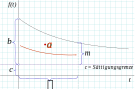
\includegraphics[width=13cm]{allg/funktionen/img/saettigung/saettigungskurveDown.png}}
\end{center}

Die Grundform eines begrenzten Zerfalls ist ein normaler
exponentieller Zerfall ($y=a^{t}$, $0<a<1$), der in $y$-Richtung um eine Sättigungsgrenze $c$ verschoben ist:

\begin{definition}{beschränkter Zerfall}{}
$$f(t) = c + b\cdot{}a^{\frac{t}{\tau}}$$
\end{definition}

Dabei ist:
\begin{itemize}
  \item $c+b = f(0) = y$-Achsenabschnitt = Startwert
	\item $c$: Die Sättigungsgrenze\index{Sättigungsgrenze} (Sättigungswert). Dies ist die Annäherungskonstante oder der \textbf{Asymtote}nwert\index{Asymptote}: Tiefer kann die Funktion nicht fallen.

	\item $m$:
    Sättigungs\textbf{differenz}\index{Sättigungsdifferenz}\index{Differenz!zur
      Sättigung}. Wie viel fehlt, bis zur
    Sättigungsgrenze: $m = f(t) - c$. Die Sättigungs\textbf{differenz} nimmt exponentiell ab.
	\item $b$: Die \textbf{Abweichung} zu $c$ zum Zeitpunkt $t=0$. Der
    Anfangswert ist somit $f(0) = c + b$; mit anderen Worten: $b$ ist das
    \textbf{Sättigungsdifferenz} zum Zeitpunkt $t_0 = 0$.

    \item $a=\frac{m}{b}=\frac{f(\tau)-c}{f(0)-c}$: Der Faktor der Veränderung der
      Sättigung\textbf{differenz}.
\end{itemize}

\subsection*{Aufgaben}
\GESOAadBMTA{359}{35. (Kuchen) und 36. (Ovomaltine)}
\olatLinkGESOKompendium{3.4.2}{33}{48. (Achtung: Das
  Kompendium verwendet andere Buchstaben: Das dortige $a$ ist unser $b$.)}

\GESO{\olatLinkArbeitsblatt{Exponentialfunktionen}{https://olat.bbw.ch/auth/RepositoryEntry/572162163/CourseNode/106029175831971}{Kap. 3.1:
    Sättigung: Begrenzter Zerfall}}
\TALS{\olatLinkArbeitsblatt{Exponentialfunktionen}{https://olat.bbw.ch/auth/RepositoryEntry/572162090/CourseNode/106029175777725}{Kap. 3.:
    Sättigung: Begrenzter Zerfall}}
\newpage


\subsection{Sättigung (begrenztes Wachstum)}\index{Sättigung}\index{begrenztes Wachstum}\index{Wachstum!begrenztes}
\subsubsection{Einstiegsbeispiel 1: Eistee wärmen}
Das Aufwärmen von Eistee von $5\degre$ Kühlschranktemperatur auf $20\degre$ Zimmertemperatur ist ein klassisches «Begrenztes Wachstum» (mit gespiegelter Exponentialfunktion).

\TNT{5.2}{Skizze}

\subsubsection{Einstiegsbeispiel 2: Batterie laden}
\begin{center}
\raisebox{-1cm}{
\includegraphics[width=8cm]{allg/funktionen/img/saettigung/batterien.png}}
\end{center}

Eine 9V-Batterie ist etwas mehr als zur Hälfte entladen und enthält nun eine
Restspannung von 4V.

Wenn wir 9V an die Batterie anlegen, so wird die Batterie geladen.

Die Batterie lädt sich umso rascher, je \textit{leerer} sie ist.

Die Batterie lädt sich umso langsamer, je \textit{voller} sie ist.


\newpage

\subsubsection{Allgemeine Form von Sättigungsprozessen}

\begin{center}
\raisebox{-1cm}{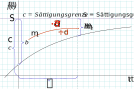
\includegraphics[width=13cm]{allg/funktionen/img/saettigung/saettigungskurve.png}}
\end{center}

Die Grundform des begrenzten Wachstums ist ein exponentieller Zerfall\totalref{zerfallsfunktion},
der an der $x$-Achse gespiegelt und in $y$-Richtung
verschoben ist:

\begin{definition}{Sättigung}{}
$$f(t) =c - b\cdot{} a^{\frac{t}{\tau}}$$
\end{definition}

Die Variable haben die folgenden Bedeutungen:

\begin{itemize}
	\item $c$: Sättigungsgrenze. Dies ist die Annäherungskonstante oder der Asymtotenwert. Höher kann die Funktion nicht steigen.

	\item $m$ ist die
    Sättigungsdifferenz\index{Sättigungsdifferenz}\index{Differenz!zur
    Sättigung}. Wie viel fehlt, bis zur
    Sättigungsgrenze: $m = c - f(t)$. Auch hier nimmt die Sättigungs\textbf{differenz} exponentiell ab.
	\item $b$: Die Abweichung des Funktionsgraphen zu $S$ zum Zeitpunkt $t=0$. Der
    Anfangswert ist somit $f(0) = c - b$.
\item $a=\frac{m}{b}=\frac{c-f(\tau)}{c-f(0)}$ Faktor der Veränderung
  der Sättigungs\textbf{differenz}.
\end{itemize}


\subsubsection{Bemerkungen}
\begin{bemerkung}{}{}
  Für die Sättigungsdifferenz gilt:

\TNT{4}{$$m = m(t) = c - f(t) = c - \left(c-b\cdot{}a^{\frac{t}{\tau}}\right) = + b\cdot{}a^{\frac{t}{\tau}}$$

und somit:

$$m_0 = m(0) = b\cdot{}a^0 = b$$}%% END TNT
\end{bemerkung}

\TRAINER{ Bemerkung (Trainer/mündlich):
  
Das $a$ kann aus zwei \textbf{beliebigen} Sättigungsdifferenz-Werten berechnet werden (die um die
Zeitdifferenz $\tau$ auseinander liegen):
$$\frac{m_2}{m_1} = \frac{b\cdot{}a^{\frac{t_2}{\tau}}}{b\cdot{}
  a^{\frac{t_1}{\tau}}} = a^{\frac{t_2}{\tau}} : a^{\frac{t_1}{\tau}} =
a^{\frac{t_2-t_1}{\tau}} = a^{\frac{\tau}{\tau}} = a$$%% 
}%% END Trainer


\begin{bemerkung}{}{}
Meistens ist $m_0$ zum Zeitpunkt $t=0$ bekannt und somit ist $b=m_0$. Es reicht, die Messung zum Zeitpunkt $t_0$ und zu einem weiteren Zeitpunkt durchzuführen. Wenn zusätzlich die Sättigungsgrenze $c$ bekannt ist, kann die Funktion $f$ komplett bestimmt werden.
\end{bemerkung} 

\newpage

\subsection{Referenzaufgaben}

\subsubsection{Berechnung am Batterie-Beispiel}\index{Batterie}
Eine Batterie weist zum Zeitpunkt $t_0$ vier Volt auf. Nach sechs Stunden am Ladegerät zeigt die Messung sieben Volt. Wir wissen, dass die Sättigungsgrenze (Ladespannung) bei neun Volt liegt.

Zeichnen Sie die gegebenen Größen in ein Koordinatensystem ein und markieren Sie bei neun Volt eine horizontale Beschränkungslinie (\zB 1V = 1 Häus'chen in $y$-Richtung; 1h = 1 Häus'chen in $x$-Richtung).

\noTRAINER{\mmPapier{8.8}}
\TRAINER{\bbwCenterGraphic{15cm}{allg/funktionen/img/saettigung/batterieFct.png}}

\textbf{Frage 1}: Wie lautet die Formel $f(t) = ...$ der Sättigungskurve?

\noTRAINER{$c = ..........................$}
\TRAINER{$c = \textrm{ Sättigungsgrenze } = 9 [\textrm{V}]$}

\noTRAINER{$b = ..........................$}
\TRAINER{$b = m_0 = c-f(0) = 9 - 4 = 5$}

\noTRAINER{$m =  ..........................$}
\TRAINER{$m = m_1 = c-f(\tau) = 9 - 7 = 2$}

\noTRAINER{$a = .........................$}
\TRAINER{$a=\frac{m}{b} = \frac{m_1}{m_0} = \frac{2}{5} = 0.4$}

\noTRAINER{$\tau = .........................$}
\TRAINER{$\tau = 6$ ($e_x$ = eine Stunde)}


\noTRAINER{$f(t) = c - b\cdot{}a^{\frac{t}{\tau}} = ..... - .....\cdot{}(.....)^{\frac{-t}{.....}}$}
\TRAINER{$f(t) = c - b\cdot{}a^{\frac{t}{\tau}} = 9 - 5\cdot{}(\frac{2}{5})^{\frac{t}{6}}$}

\TRAINER{Die Kontrollen für $t=0$ und $t=6$ sind mit dem Stehenlassen von $a$ als Bruch nun sehr einfach.}
\newpage

\textbf{Frage 2}: Wann wird die Batterie zu 99\% geladen sein?

\TNTeop{99\% von 9V = 8.91 V

  Somit ist $t$ gesucht mit $f(t) = 9 - 5\cdot{}\left(\frac25\right)^{\frac{t}{6}} = 8.91$

  (beidseitig -9 und Vorzeichen drehen und dann durch 5 teilen, so folgt...)

  $$(0.4)^{\frac{t}{6}} = (9-8.91) : 5 = 0.09 : 5 = 0.018$$

  Definition Logarithmus:

  $$\frac{t}6 = \log_{0.4}(0.018) \approx 26.3 $$

  Nach ca. 26 - 27 Stunden ist die Batterie zu 99\% geladen.
}
\newpage

\subsubsection{Referenzaufgabe Sättigung: Pneu}\index{Reifen}\index{Pneu}

Ein Reifen (Pneu) ist anfänglich ganz leer und enthält «nur» 1 atm, nämlich den
Druck der Umgebung. (1 atm = atmosphärischer Druck = technische Atmosphäre) 

Der Reifen wird aufgepumpt mit einer Druckpumpe, die maximal 2 atm
leisten
kann. Mit 2 atm ist hier gemeint: 2 at mehr als der
Umgebungsdruck. Somit könnte der Pneu bis auf maximal 3 atm aufgepumpt
werden (= Sättigungsgrenze).

Um den Reifen optimal zu füllen, wird er auf 2 atm aufgepumpt (1 atm
über dem Umgebungsluftdruck).

Die Pumpe schafft in den ersten 10 Sekunden den Druck von 1 atm auf 1.2
atm (= 0.2 atm über Normaldruck) aufzupumpen.

Nach wie vielen Sekunden muss gestoppt werden, damit der Reifen
optimal gepumpt ist?

\TNTeop{Die Sättigungsdifferenz schwindet von $m_1=3-1=2$ bis $m_2=3-1.2=1.8$
innerhalb der ersten $10s = \tau$. Die Sättigungsgrenze liegt bei
$S=3$. Unsere (Exponential)basis $a$ ist somit $1.8 / 2$, was uns
liefert:
$$f(t) = 3 - 2\cdot{}\left(\frac{1.8}{2}\right)^\frac{t}{10}$$
Somit ist das Optimum bei $2 = 3-
2\cdot{}\left(\frac{1.8}{2}\right)^\frac{t}{10}$ erreicht, also bei
etwa 65.8 Sekunden.
}
\newpage

\GESO{\subsection*{Aufgaben}}
\GESOAadBMTA{358}{34. (Eistee)}
\olatLinkGESOKompendium{3.4.2}{32ff}{49. - 51. (Bem.: Das
  Kompendium gibt die Funktionsterme bereits an und verwendet als
  Basis i.\,d.\,R. die Eulersche Konstante $e\approx{} 2.71828$)}

\GESO{\olatLinkArbeitsblatt{Exponentialfunktionen}{https://olat.bbw.ch/auth/RepositoryEntry/572162163/CourseNode/106029175831971}{Kap. 3.1:
    Begrenztes Wachstum}}%% END GESO
\TALS{\olatLinkArbeitsblatt{Exponentialfunktionen}{https://olat.bbw.ch/auth/RepositoryEntry/572162090/CourseNode/106029175777725}{Kap. 3.1:
    Begrenztes Wachstum}}%% END TALS

\newpage

\subsection{Zusammenfassung der Prozesse}
\vspace{8mm}
\begin{center}\textbf{Wachstum und Zerfall}\end{center}

\TNT{8.8}{\bbwCenterGraphic{18cm}{allg/funktionen/img/zusammenfassung_exp/wachstum_zerfall.png}

  bzw.
  $$f(t) = G_0 \cdot{} \e^{qt}; q=  \frac{\ln(a)}\tau  \,\,\,\,\,\,\,\,\, f(t) = G_0 \cdot{} \e^{-qt}; q  = \frac{-\ln(a)}\tau$$
}%% END TNT

\vspace{8mm}
\begin{center}\textbf{Sättigung}\end{center}

\TNTeop{\bbwCenterGraphic{18cm}{allg/funktionen/img/zusammenfassung_exp/saettigung.png}

    bzw.
     $$f(t) = S + (G_0-S) \cdot{} \e^{q\cdot{}t}; q=    \frac{\ln(a)}\tau     \,\,\,\,\,\,\,\,\, f(t) = S + (S - G_0) \cdot{} \e^{-q\cdot{}t}; q  = \frac{-\ln(a)}\tau$$

Hier ist Platz für das Video/die Videos zur den getanzten
Funktionen (S. OLAT/Wiki).
}%% END TNTeop

\newpage

\TALS{
  \subsection*{Aufgaben}
  \olatLinkTALSStrukturaufgabenSPF{Basiskenntnisse Funktionen Teil
    1}{5}{4., 5., 8. und 9.}
  \olatLinkTALSStrukturaufgabenSPF{Basiskenntnisse Funktionen Teil
    2}{14}{45., 47. und 49.}
}%% END TALS
\newpage


%%%%%%%%%
%% Gleichungen II
%%%%%%%%%%%%%%%55
%% Funktionen II GESO Metapackage
\part{Funktionen II}\index{Funktionen!II|textbf}
\renewcommand{\bbwPartID}{FCT2}
\section{Potenzfunktionen}\index{Funktion!Potenzfunktionen}\index{Potenzfunktionen}
\sectuntertitel{Funktionen hoch drei!}

\subsection*{Lernziele}

\begin{itemize}
\item Definition Ganzzahlige Potenzfunktion
\item Graphische Darstellung
\end{itemize}
\newpage


\subsection{Einstieg}

%%%%%%%%%%%%%%%%%%%%%%%%%%%%%%%%%%%%%%%%%%%%%%%%%%%%%%%%%%%%%%%%%
\subsubsection{Beispiel: Rationale Funktion\GESO{ (optional)}}

Betrachten wir einmal die Funktion $f: y = 0.1x^3 + x^2 + 2x + 3 - x^{-1}$ \zB mit Geogebra (\texttt{www.geogebra.org}).

\bbwGraph{-10}{4}{-7}{8}{%
  \bbwFunc{0.1*\x*\x*\x + \x*\x + 2*\x + 3 -1/\x}{-8.5:-0.2}
  \bbwFunc{0.1*\x*\x*\x + \x*\x + 2*\x + 3 -1/\x}{0.1:1.5}
}%%


Polynomfunktionen und rationale Funktionen sind «\textit{weiche}» Funktionen, die jedoch \textbf{Asymptoten}\index{Asymptote} (hier bei $x=0$) aufweisen können.
Ebenso sind die Extremwerte (lokale Maxima und Minima)\TALS{ wie auch die Wendepunkte} charakteristische Stellen und oft Gegenstand der Untersuchung.
Wir beschränken uns \TALS{vorerst }auf Funktionen der Art $f: y=a\cdot{}x^z$
mit $z \in \mathbb{Z}\backslash\{0\}$\TRAINER{ $z=0$ ist eine
  Proportionalität und somit hier unspannend}.

\newpage



\subsubsection{\GESO{Beispiel}\TALS{Repetition}: Reinquadratische Funktion}\index{quadratische Funktion}\index{Funktion!quadratische}

Zeichnen Sie den Graphen der Funktion $f: y= \frac16 x^2$:

\bbwGraph{-7}{7}{-1}{6.5}{%%
  \TRAINER{
    \bbwFunc{\x*\x/6}{-6:6}
  }
}%%

\begin{definition}{Reinquadratische Funktion}{}
Die Funktion

$f: y = a\cdot{}x^2$

heißt \textbf{Parabel zweiter Ordnung} oder rein-quadratische Funktion.
\end{definition}


\TALS{
\begin{bemerkung}{}{}
Eine allgemeine quadratische Funktion besitzt auch noch einen linearen ($bx$) und einen konstanten ($c$) Anteil. Die allgemeine quadratische Funktion hat die Form

$$f: y= ax^2 + bx + c$$
\end{bemerkung}
}%% END TALS

\TALS{Beispiele zu allgemeinen quadratischen Funktionen finden sie im
  Buch \cite{marthaler21alg} ab Seite 260 insb. im Bild zu Aufg. 4 auf
  Seite 273.}%% END TALS

\newpage

\subsection{Parabel}\index{Parabel}

Zeichnen Sie $y = \frac{1}{16}x^4$ im Bereich $[-3; 3]$ indem Sie für jeden 0.5-er $x$-Wert das zugehörige $y$ berechnen:

\bbwGraph{-4}{4}{-1}{6.5}{%%
  \TRAINER{\bbwFunc{\x*\x*\x*\x/16}{-3:3}}
}%%


\begin{definition}{Parabel}{definition_parabel}
  Ist $n\in \mathbb{N}_{\ge 2}$, so wird der Graph der Potenzfunktion
  $$x\mapsto a\cdot{}x^n$$
  \textbf{Parabel} $n$-ter Ordnung genannt.
\end{definition}

\TALS{%%
\begin{bemerkung}{Potenzfunktion}{definition_potenzfunktion}
  Eine Funktion der Art
$$f: y=a\cdot{}x^r$$
  mit $r \in \mathbb{R}\backslash\{0\}$ heißt \textbf{Potenzfunktion}.
\end{bemerkung}

\begin{bemerkung}{Polynomfunktionen}{}
  Funktionen, deren Funktionsterm ein Polynom bilden werden
  \textbf{Polynomfunktionen} genannt:
  $$f: y=a_n\cdot{}x^n + a_{n-1}\cdot{}x^{n-1} + a_{n-2}\cdot{}x^{n-2} + ... + a_2\cdot{}x^2 + a_1 \cdot{} x + a_0 $$
\end{bemerkung}
%
}%% END TALS


\newpage
\subsection*{Aufgaben}
\aufgabenFarbe{Zeichnen Sie die Parabeln $$y=f(x) = x^n$$ für $n = 2$,
  $n=3$, $n=4$, $n=5$ und $n=6$ mit \texttt{geogebra.org}.
\\
Was fällt auf?}
%%\GESOAadBMTA{303ff}{1. (nur $n=3$ und $n=5$), 2. (nur $n=4$ und $n=6$)}

\TNTeop{}

\newpage

\subsubsection{Anwendung (optional)}
Boltzmannsches T-hoch-vier-Gesetz\index{Boltzmann!$T^4$-Gesetz}

\leserluft{}

Die Funktion $P(T) = \sigma\cdot\varepsilon\cdot
  A\cdot{}T^4$ beschreibt, welche Strahlungsleistung $P$ ein Körper der
  Oberfläche $A$ (in $ \text{m}^2$) bei Temperatur $T$ (in Kelvin) aussendet.

  $\sigma$ = Bolzmann Konstante = $5.6\cdot{}10^{-8}$
  
  $\varepsilon$ = Emissionswert

  \small{\texttt{(eg. https://ennologic.com/wp-content/uploads/2018/07/Ultimate-Emissivity-Table.pdf)}}

  \leserluft{}
  
  Rechenbeispiel:

\TNTeop{$T$ = 20 Grad Zimmertemperatur in Kelvin: 293.15;
  Brick (Haus) hat Emissionswert ca. 0.75; Haus Oberfläche $500 \text{m}^2$

  $$P(293.15) \approx 5.6\cdot{}10^{-8} \cdot{} 0.75 \cdot{} 500
  \cdot{} 293.15^4 \approx 155 \text{kW} $$
  Natürlich strahlt eine 20-grädige Umgebungstemperatur gleich viel
  wieder zurück, sodass keine 'Heizkosten' entstehen.

  Heizen wir das Haus nun zwei Grad wärmer, so erhalten wir:
  $$P(295.15) \approx 5.6\cdot{}10^{-8} \cdot{} 0.75 \cdot{} 500
  \cdot{} 295.15^4 \approx 159.4 \text{kW} $$

  Dies entspricht einer Differenz von 4.28 kW für nur zwei Grad wärmer
  im Haus!
  

}%% END TNT
\newpage

Zeichnen Sie des weiteren die Funktion $y = \frac{1}{9}x^3$:

\bbwGraph{-4}{4}{-5}{5}{%%
  \TRAINER{\bbwFunc{\x*\x*\x/9}{-3.5:3.5}}
}%%

\subsubsection{Symmetrien}\index{Symmetrien!von Parabeln}\index{Parabel!Symmetrie}
Was fällt für gerade und ungerade Exponenten auf? Gibt es Spiegelachsen
oder Spiegelpunkte?

\renewcommand{\mmPapier}[1]{\mmPapierZwei{#1}{16.4}}
\begin{tabular}{c|p{8cm}}
  $x^2$ & \vspace{0.1mm}\TNT{0.8}{An der $y$-Achse}\\\hline
  $x^3$ & \vspace{0.1mm}\TNT{0.8}{Am Ursprung $O(0|0)$}\\\hline
  $x^4$ & \vspace{0.1mm}\TNT{0.8}{wie $x^2$}\\\hline
  $x^5$ & \vspace{0.1mm}\TNT{0.8}{wie $x^3$}\\\hline
\end{tabular}
\renewcommand{\mmPapier}[1]{\mmPapierZwei{#1}{17.6}}


\GESO{Eine Zusammenfassung der wichtigsten Eigenschaften von
  Potenzfunktionen finden Sie im Buch \cite{marthaler21alg} Seite 296 oben.}
\newpage

\subsubsection{Referenzaufgabe}

Bestimmen Sie $a$ und $k$ so, dass der Graph von $y = a \cdot{} x^k$
durch die Punkte $P=\left(3 \middle| 1458\right)$ und
$Q=\left(-4\middle|8192\right)$ verläuft.

\TNT{15.2}{ Punkte einsetzen in die Funktionsgleichung:
  \gleichungZZ{1458}{a\cdot{}3^k}{8192}{a\cdot{}(-4)^k}
  Aus der oberen Gleichung das $a$ ermitteln ($a=\frac{1458}{3^k}$)
  (I) und in die zweite
  Gleichung einsetzen: $$8192 = \frac{1458}{3^k} \cdot{} (-4) ^k$$
  Exponent $k$ separieren:
  $$\frac{8192}{1458} = \left(\frac{-4}3\right)^k$$
  Problem: Logarithmen mit negativen Basen (hier $\frac{-4}3$)
  funktionieren nicht!
  
  Weil nun $k$ gerade sein muss, folgt dass $\left(\frac{-4}3\right)^k
  = \left(\frac43\right)^k$. Daraus ergibt sich
  $$\frac{8192}{1458} = \left(\frac{4}3\right)^k \Longrightarrow k =
  \log_{\frac43}\left(\frac{8192}{1458}\right) = 6$$
  Dieses $k$ nun in die Gleichung (I) einsetzen; dies
  liefert
  $$a=\frac{1458}{3^k} = 2.$$
}%% end TRAINER


\subsection*{Aufgaben}
\AadBMTA{305ff}{11. a) b) c), 13. a) c), (optional 17.,)  18.}
%%\TALSAadBMTA{197}{735. (6) (7) und (9) jeweils mit geogebra, 736. a) d),
%%  737. a) c), 739.}
\newpage


\subsection{Translationen}\index{Manipulation!Funktionen}\index{Funktions-Manipulation}\index{Translation!Funktion}
\sectuntertitel{Manipulation an Funktionsgraphen}
(Verschiebung\index{Verschiebung}, Spiegelung\index{Spiegelung},
Streckung\index{Streckung})

\TadBMTA{217}{13.3}
%%\TALSTadBFWA{163}{3}
Betrachten Sie die Funktionen

$$f(x) = a\cdot{}\left(\frac{x\TALS{-d}}b\right)^5\TALS{+c}$$
und
$$g(x) = a\cdot{}\left(\frac{x\TALS{-d}}b\right)^4\TALS{+c}$$

mit Geogebra (\texttt{geogebra.org})
und beschreiben Sie die Effekte der Parameter

$a$: \TRAINER{Streckung in $y$-Richtung. $a$ negativ: Spiegelung an der
$x$-Achse.}

\noTRAINER{\mmPapier{2.4}}

$b$: \TRAINER{Streckung entlang der $x$-Achse. $b$ negativ: Spiegelung
  an der $y$-Achse.}

\noTRAINER{\mmPapier{2.4}}

\TALS{%% nur TALS haben Verschiebungen
  $c$: \TRAINER{Verschiebung entlang der $y$-Achse}

\mmPapier{2.4}
}%% end TALS

\TALS{
$d$: \TRAINER{Verschiebung entlang der $x$-Achse (Verschiebung nach
  rechts verlangt ein negatives $d$.)}

\noTRAINER{  \mmPapier{2.4}}
}%% END TALS

\newpage

\subsubsection{Zusammenfassung der Translationen}


Wir betrachten die verschiedenen geometrischen
Funktions-«Manipulationen» (Abbildungen) am Beispiel {\color{red}$y =f(x) = \frac18 x^3$}.


\newcommand{\graphTranslationMultiColumn}[5]{%
  \multicolumn{3}{|l|}{#1}\\%%
\hline%%
\graphTranslationMultiColumnZ{#2}{#3}{#4}{#5}
}%% end new command \graphTranslationMultiColumn

\newcommand{\graphTranslationMultiColumnZ}[4]{%
\multirow{5}{6cm}{#1} &  & \multirow{2}{*}{\begin{minipage}{.3\textwidth}\raisebox{-8cm}{\includegraphics[width=\linewidth,height=60mm]{allg/funktionen/img/translation/#4}}\end{minipage}}\\[55mm]%%
&\fbox{#2}&\\%%
&&\\%%
&{\color{red}\fbox{#3}}&\\%%
&&\\%%
\hline%%
}%% end new command \graphTranslationMultiColumnZ

\TALS{%% Nur TALS haben Verschiebungen
\begin{tabular}{|p{7cm}|c|c|}%%
\hline%%
\graphTranslationMultiColumn{Verschiebung in $y$-Richtung...}{... um \textbf{zwei} Einheiten nach \textbf{oben}:}{$g(x)=f(x)\textbf{+2}$}{$g(x)=\frac18x^3\textbf{+2}$}{typ1.png}
\graphTranslationMultiColumnZ{... um \textbf{eine} Einheiten nach \textbf{unten}:}{$g(x)=f(x)\textbf{-1}$}{$g(x)=\frac18x^3\textbf{-1}$}{typ2.png}
\end{tabular}%%
}%% end TALS

\begin{tabular}{|p{7cm}|c|c|}%%
\hline%%
\graphTranslationMultiColumn{Spiegelung...}{... an der $x$-Achse:}{$g(x)=-f(x)$}{$g(x)=-\frac18x^3$}{typ3.png}
\graphTranslationMultiColumnZ{... an der $y$-Achse:}{$g(x)=f(-x)$}{$g(x)=\frac18(-x)^3$}{typ4.png}
\end{tabular}%%

\begin{tabular}{|p{7cm}|c|c|}%%
\hline%%
\graphTranslationMultiColumn{Streckung...}{... in $y$-Richtung (von der $x$-Achse aus) um Faktor \textbf{zwei}:}{$g(x)=\textbf{2}\cdot{}f(x)$}{$g(x)=\textbf{2}\cdot{}\frac18x^3$}{typ5.png}
\graphTranslationMultiColumnZ{... in $x$-Richtung (von der $y$-Achse aus) um Faktor \textbf{zwei}:}{$g(x)=f(\frac{1}{\textbf{2}}\cdot{}x)$}{$g(x)=\frac18(\frac{1}{\textbf{2}}\cdot{}x)^3$}{typ6.png}
\end{tabular}%%

\TALS{%% Nur TALS verschieben in x-Richtung
\begin{tabular}{|p{7cm}|c|c|}%%
\hline%%
\graphTranslationMultiColumn{Verschiebung in $x$-Richtung\footnote{Kein prüfungsrelevantes Thema.}...}{... um \textbf{zwei} Einheiten nach \textbf{links}:}{$g(x)=f(x\textbf{+2})$}{$g(x)=\frac18(x\textbf{+2})^3$}{typ7.png}
\graphTranslationMultiColumnZ{... um \textbf{zwei} Einheiten nach \textbf{rechts}:}{$g(x)=f(x\textbf{-2})$}{$g(x)=\frac18(x\textbf{-2})^3$}{typ8.png}
\end{tabular}%%
}%% END TALS
\newpage

\subsection*{Aufgaben}
\GESO{
Skizzieren Sie $-\frac{1}{2}x^3 - 1$ im Bereich $x$ = -2 bis $x$ = +2.

\bbwGraph{-4}{4}{-5}{3}{%%
  \TRAINER{%
    \bbwFunc{-0.5*\x*\x*\x-1}{-2:2}%
  }%%
}%

Vergleichen Sie die neue Funktion mit der Parabel $y=x^3$.

\TNT{5.2}{Die neue Funktion ist an der $y$-Achse gespiegelt, ist um
  50\% gestaucht ($y$-Richtung) und ist um eine Einheit nach unten
  ($x$-Richtung) verschoben worden.}
}%% END GESO

\AadBMTA{304ff}{5. a) c) d) e), 9. a) d) e)}

 
\TALS{
  \aufgabenFarbe{Zeichnen Sie mit \texttt{geogebra.org} die Funktion
    $f(x) = \frac1{10}(x^3 - 3x^2 + 3)$
    \\
    Definieren Sie anschließend die Funktion $$g(x) = a\cdot{}f((x+s)\cdot{}b)+r.$$
\\
    Entscheiden Sie, welche Veränderungen die Parameter $a$, $b$, $r$
    und $s$ bewirken.\\
    Starten Sie mit $a=1$, $b=1$, $r=0$ und $s=0$.
  }%% END Aufgabenfarbe
  \TNT{4}{
    $r$: Verschiebung nach oben\\
    $s$: Verschiebung nach links\\
    $a$: Streckung in $y$-Richtung\\
    $b$: Stauchung in $x$-Richtung
  }%% END TNT
}%% END TALS



%%  OLAT Arbeitsblatt
\GESO{\olatLinkArbeitsblatt{Positive Potenzfunktionen zuordnen}{https://olat.bbw.ch/auth/RepositoryEntry/572162163/CourseNode/104752086007823}{(alle Beispiele)}}%% END olatLinkArbeitsblatt
\TALS{\olatLinkArbeitsblatt{Positive Potenzfunktionen zuordnen}{https://olat.bbw.ch/auth/RepositoryEntry/572162090/CourseNode/105597875231723}{(alle Beispiele)}}%% END olatLinkArbeitsblatt


\olatLinkTALSStrukturaufgabenSPF{Teil 2}{15ff}{48. und 51.}
%%\TALS{\aufgabenFarbe{Strukturaufgaben SPF Teil 2: Taschenrechner: S. 15ff:  Aufg. 48. und 51.}%% END Aufgabenfarbe
%%}%% END TALS

%%\TALSAadBMTA{197 ff.}{739., 743. c), 745. c), 738.*}

\olatLinkGESOKompendium{3.3.1.}{26}{28., 29.}
\newpage



%%%%%%%%%%%%%%%%%%%%%%%%%%%%%%%%%%%%%%%%%%%%%%%%%%%%%%%%%%%%%%%%%%%%%%%%%%%%%%%%%%%
\subsection{Hyperbel}\index{Hyperbel (negative Exponenten)}

(«Hyperbel» Griechisch = «über das Ziel hinaus werfen»)


Zur Erinnerung:
\begin{multicols}{2}
\begin{itemize}
	\item $x^{-1} = \frac{1}{x}$
	\item $x^{-2} = \frac{1}{x^2}$
	\item $x^{-3} = \frac{1}{x^3}$
	\item $x^{-4} = \frac{1}{x^4}$
	\item $x^{-5} = \frac{1}{x^5}$
  \item ...
\end{itemize}
\end{multicols}

Zeichnen Sie die Funktion $f: y = x^{-1}$ im Definitinosbereich
$\DefinitionsMenge{} = [-5;5]\TRAINER{\backslash \{0\}}\noTRAINER{......}$

\bbwGraph{-6}{6}{-3}{3}{%%
  \TRAINER{\bbwFunc{1/\x}{-5:-0.3}}
  \TRAINER{\bbwFunc{1/\x}{0.3:5}}

}%%

\newpage


Zeichnen Sie zusätzlich Funktion $f: y = x^{-2}$ im Definitionsbereich $[-5;5]$:

\bbwGraph{-6}{6}{-5}{5}{%%
  % x^-2
  \TRAINER{\bbwFuncC{1/(\x * \x)}{-5:-0.447}{green}}%% 0.447 = 1/sqrt (5)
  \TRAINER{\bbwFuncC{1/(\x * \x)}{0.447:5}{green}}
  \TRAINER{\bbwLetter{2.5,0.5}{x^{-2}}{green}}
  \TRAINER{\bbwLetter{-1.5,1}{x^{-2}}{green}}

  %x^-3
%  \TRAINER{\bbwFuncC{1/(\x * \x * \x)}{-5:-0.584}{blue}}
%  \TRAINER{\bbwFuncC{1/(\x * \x * \x)}{0.584:5}{blue}}
%  \TRAINER{\bbwLetter{0.8,0.3}{x^{-3}}{blue}}
%  \TRAINER{\bbwLetter{-1.2,-3.8}{x^{-3}}{blue}}
%  \TRAINER{\bbwLetter{1.2,4.5}{x^{-3}}{blue}}

}%%

\begin{definition}{Hyperbel}{definition_hyperbel}
  Der Graph einer Potenzfunktion $$f: y=ax^z$$
  mit $z \in \{-1, -2, -3, -4, ...\}$ heißt
\textbf{Hyperbel}\index{Hyperbel} der Ordnung $z$.
\end{definition}

Der Definitionsbereich von Hyperbeln entspricht dem Definitionsbereich
des Funktionsterms. Merke: Es darf nicht durch Null geteilt werden:

$$x^{-5} = \frac{1}{x^5} \Longrightarrow \DefinitionsMenge{} = \mathbb{R} \backslash \{0\}$$


\subsection*{Aufgaben}
\AadBMTA{306ff}{19. Zeichnung mit geogebra.org, 20.
  Zeichnung mit geogebra.org}
%%\TALSAadBMTA{205}{771. a) c) d) e) g) h) j)}


\newpage

\subsubsection{Charakteristiken}
\textbf{Spiegelungen:}\\

Welche Funktionen $x$, $x^{-1}$, $x^{-2}$, $x^{-3}$ sind an welchen Achsen bzw. Punkten gespiegelt?

\renewcommand{\mmPapier}[1]{\mmPapierZwei{#1}{16.0}}
\begin{tabular}{c|p{10cm}}
  $x^{-1}$ &  \TNT{0.8}{Am Ursprung $O(0|0)$ : Punktspiegelung}\\
  \hline
  $x^{-2}$ &  \TNT{0.8}{An der $y$-Achse: Achsensymmetrie}\\
  \hline
  $x^{-3}$ &  \TNT{0.8}{Am Ursprung $O(0|0)$: Punktspiegelung}\\
  \hline
  $x^{-4}$ &  \TNT{0.8}{An der $y$-Achse: Achsensymmetrie}\\
  \hline  
\end{tabular}
\renewcommand{\mmPapier}[1]{\mmPapierZwei{#1}{17.6}}


\paragraph{Definitions- und Wertebereiche:}

Geben Sie für die obigen Funktionen an, was ihr Definitions- bzw. Wertebereich ist\footnote{Grundmenge ist $\mathbb{R}$.}:

\begin{tabular}{c|c|c}
Funktionsterm & Definitionsbereich $\DefinitionsMenge{}$& Wertebereich $\Wertebereich{}$\\ \hline
  $x^{-1}$ & \TRAINER{$\mathbb{R}\backslash\{0\}$} &  \TRAINER{$\mathbb{R}\backslash\{0\}$}\\ \hline
  $x^{-2}$ & \TRAINER{$\mathbb{R}\backslash\{0\}$} &  \TRAINER{$\mathbb{R}^{+}\backslash\{0\}$}\\ \hline
  $x^{-3}$ & \TRAINER{$\mathbb{R}\backslash\{0\}$} &  \TRAINER{$\mathbb{R}\backslash\{0\}$}\\ \hline
  $x^{-4}$ & \TRAINER{$\mathbb{R}\backslash\{0\}$} &  \TRAINER{$\mathbb{R}^{+}\backslash\{0\}$}\\ \hline
\end{tabular}


\GESO{\subsection*{Aufgaben}}
\olatLinkGESOKompendium{3.3}{26}{28. bis 31.}
\GESO{\aufgabenFarbe{Aufgabe der Nullserie 2 (zweite Nullserie): Aufg. 7 auf Seite 3}}
\GESO{\aufgabenFarbe{Maturaprüfung 2016, Aufg. 8 (Graphen zuordnen)}}

\newpage

\newpage

%%%%%%%%%%%%%%%%%%%%%%%%%%%%%%%%%%%%%%%%%%%%%%%%%%%%%%%%%%%%%%%%%%%%%%%%%%%%%%%%%%%

\subsection{Zusammenfassungen und Überblick}\index{Potenzfunktionen!Überblick}

$$y = a\cdot{}x^z$$

$z$ gerade: Gespiegelt an der $y$-Achse

$z$ ungerade: Gespiegelt am Ursprung $O=(0|0)$

Ist ${\color{ForestGreen}a>0}$\TRAINER{ (grün in der Graphik)}, so sind Graphen mit
geraden Exponenten nach oben geöffnet bzw. mit ungeraden Exponenten im
Quadranten I und III.

Ist ${\color{red}a<0}$\TRAINER{ (rot/orange in der Graphik)}, so sind Graphen mit
geraden Exponenten nach unten geöffnet bzw. mit ungeraden Exponenten
im Quadranten II und IV.


\TRAINER{%
  \includegraphics[width=8.5cm]{allg/funktionen/img/potenzfct/potenzFunktionenGerade.png}\hfill{}\includegraphics[width=8.5cm]{allg/funktionen/img/potenzfct/potenzFunktionenUngerade.png}
}%% END Trainer
\noTRAINER{%
  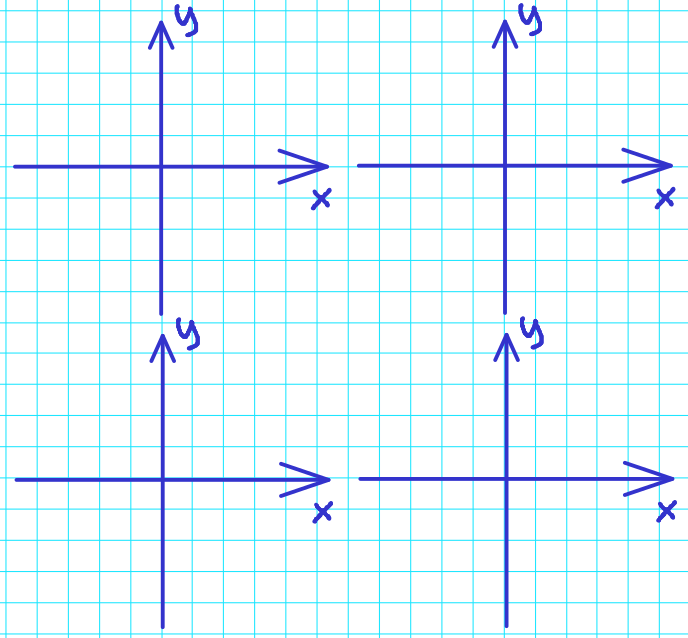
\includegraphics[width=8.5cm]{allg/funktionen/img/potenzfct/potenzFunktionenLeer.png}\hfill{}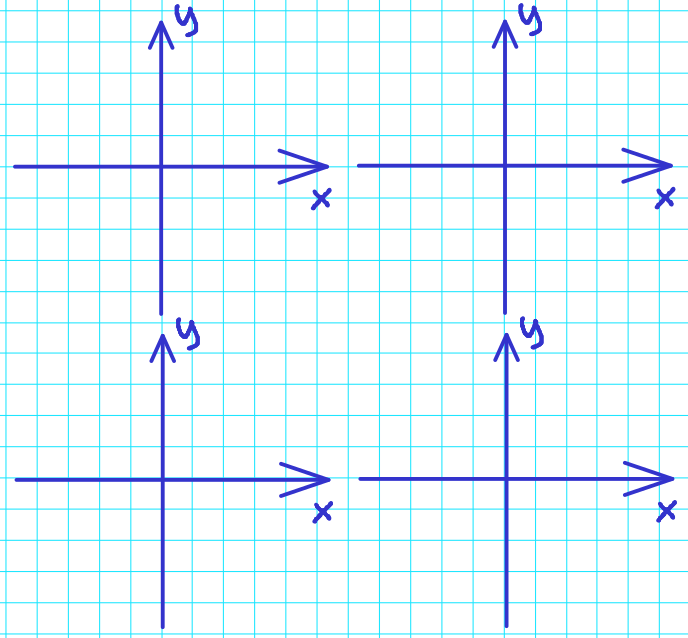
\includegraphics[width=8.5cm]{allg/funktionen/img/potenzfct/potenzFunktionenLeer.png}
}%% END Trainer


\subsection*{Aufgaben}
\AadBMTA{307}{25. b) c), 26. a)\TALS{ b)}, 27. b) c)\TALS{, 33*}}

\newpage


\newpage
\newpage
%%
%% 2019 07 04 Ph. G. Freimann
%%

\section{Exponentialfunktionen}\index{Funktion!Exponentialfunktion}\index{Exponentialfunktionen}
\sectuntertitel{Go viral!}
%%%%%%%%%%%%%%%%%%%%%%%%%%%%%%%%%%%%%%%%%%%%%%%%%%%%%%%%%%%%%%%%%%%%%%%%%%%%%%%%%
\subsection*{Lernziele}

\begin{itemize}
\item Definition Exponentialfunktion
\item Koeffizienten interpretieren
\item Graph: Symmetrien, Polstellen, Asymptoten, Schnittpunkte mit
  Achsen
  \item Basiswechsel
\end{itemize}

\TadBMTA{322}{19}
%%\TALS{(\cite{frommenwiler17alg} S.215 (Kap. 3.10))}
%%\GESO{(\cite{marthaler21alg}       S.322 (Kap. 19))}
\newpage

\subsection{Aussehen von Exponetialfunktionen}


Zeichnen Sie $f: y=2^x$ und $g: y=1.4^x$ ins selbe Koordinatensystem:


\bbwGraph{-5}{5}{-1}{5}{
\TRAINER{  \bbwFuncC{pow(2.0,\x)}{-3.5:2.1}{blue}
  \bbwFuncC{pow(1.4,\x)}{-3.5:3}{green}
  \bbwLetter{1,3}{$f$}{blue}
  \bbwLetter{2.5,2}{$g$}{green}
}%% end TRAINER
}%% end graph

\begin{definition}{Exponentialfunktion}{}\index{Exponentialfunktionen!Definition}
  Eine Funktion der Form $$f(x): x \mapsto a^x$$
  bzw. $$y = a^x$$
  mit $a\in \mathbb{R}^{+}\backslash\{1\}$ heißt \textbf{Exponentialfunktion}.
\end{definition}


\begin{bemerkung}{Zunahmefaktor}{}\index{Zunahmefaktor|textbf}
Der Parameter $a$ gibt den Wachstumsfaktor pro Zeiteinheit $e_x$ an.
\end{bemerkung}


\subsubsection*{Aufgaben}
\GESO{\olatLinkArbeitsblatt{Exponentialfunktionen}{https://olat.bms-w.ch/auth/RepositoryEntry/6029794/CourseNode/106029175831971}{Kap. 1.2:
    Einfache Wachstumsprozesse: Aufgaben 4. bis 6.}}
\TALS{\olatLinkArbeitsblatt{Exponentialfunktionen}{https://olat.bms-w.ch/auth/RepositoryEntry/6029786/CourseNode/106029175777725}{Kap. 1.2:
    Einfache Wachstumsprozesse: Aufgaben 4. bis 6.}}

\newpage

\subsection{Formen der Darstellung}
Zeichnen Sie die Funktionen $f: y=2^x$, $g: y=2^{-x}$ und $h: y=\left(\frac12\right)^x$ in dasselbe Koordinatensystem:

\bbwGraph{-6}{6}{-1}{5}{
  \TRAINER{\bbwFuncC{exp(0.69314718*\x)}{-6:2}{blue}}
  \TRAINER{\bbwFuncC{exp(-0.69314718*\x)}{-2:6}{red} }
  \TRAINER{\bbwLetter{1.5,4}{2^x}{blue}}
  \TRAINER{\bbwLetter{-5,4}{g(x)=2^{-x}=\left(\frac{1}{2}\right)^x=h(x)}{red}}
}

Bemerkung: \TRAINER{$$2^{-x} = \frac1{2^x} = \frac{1^x}{2^x}= \left(\frac12\right)^x$$}
\newpage



\subsubsection{Umkehrung (Optional)}
Um aus einem Wachstum einen Zerfall zu modellieren können wir entweder
die Zeitachse umdrehen oder den Kehrwert der Basis verwenden.
umgedreht werden:

Mit $d := \frac1a $ gilt:

\begin{center}
  \fbox{$a^{+t} = \left(\frac1a\right)^{-t} = d^{-t} $}
\end{center}

\newpage

\newpage

\subsection{Verschiebung und Streckung \GESO{(optional)}}

Eine Verschiebung der Exponentialfunktion $y=b\cdot{}a^x$ in der Zeit ($x$-Richtung) kann auch in Form einer Veränderung der Startfaktors $b$ umgeschrieben werden.

Verschieben wir \zB $$y=2^x$$ um fünf Einheiten nach rechts, so liest sich die neue Funktionsgleichung wie folgt:
$$y=2^{x-5}.$$

(Zeichnen Sie in \texttt{geogebra.org} a) $y=2^x$ und b) $y=2^{x-5}$.)

Dies kann jedoch auch umgeschrieben werden:

$$2^{x-5} = 2^x \cdot{} 2^{-5} = 2^{-5} \cdot{} 2^x = \frac{1}{2^5} \cdot{} 2^x =
\frac{1}{32}\cdot{}2^x$$

\bbwCenterGraphic{8cm}{allg/funktionen/img/exp/verschiebung_gleich_streckung.png}
Bildlegende: Eine Verschiebung ($x$-Richtung) der Exponentialfunktion entspricht einer Stauchung ($y$-Richtung) der selben Exponentialfunktion.

\TALS{Es gilt hier $$a^{x-b}=\frac{a^x}{k}$$ mit
$k=a^b$ und mit $b=\log_a(k)$.}

\newpage


\subsection{Punkte einsetzen\GESO{ (optional)}}
Wie bei den linearen Funktionen oder bei den Potenzfunktionen können auch Exponentialfunktionen gefunden werden, wenn bereits Punkte auf dem Graphen bekannt sind:

\textbf{Referenzaufgabe}

Finden Sie die Parameter $a$ und $b$ der Exponentialfunktion
$$f: y=b\cdot{}a^x$$
wenn Sie wissen, dass die Funktion durch die Punkte $P=(2|4)$ und $Q=(-1|2)$ verläuft:

\TNTeop{
  In Gleichung einsetzen:

  \gleichungZZ{4}{b\cdot{}a^2}{2}{b\cdot{}a^{-1}}

  Einsetzverfahren: Zum Beispiel aus der zweiten Gleichung das $b$ ermitteln...
  $$b = 2 a (III)$$
  ... und in die erste Gleichung einsetzen:

$$4 = 2a\cdot{} a^2$$
  $$2 = a^3$$
  $$a=\sqrt[3]{2}$$
  In (III) einsetzen:

  $$b = 2 \sqrt[3]{2}$$

  Ergo: $$f(x) = b\cdot{}a^x = 2\cdot{}\sqrt[3]{2} \cdot{} \left(\sqrt[3]2\right)^x \approx 2.5198 \cdot{} 1.2599^x$$
}

\subsection*{Aufgaben}
%%\AadBMTA{334}{10. a) b)\TALS{ e)}\GESO{ f)}}
\GESO{\olatLinkArbeitsblatt{Exponentialfunktionen}{https://olat.bms-w.ch/auth/RepositoryEntry/6029794/CourseNode/106029175831971}{Kap. 2.1: E-Funktion / Punkte-Aufgaben Aufg 26. a) b) ($e^{qt}$ optional) und Aufg. 27.}}
\TALS{\olatLinkArbeitsblatt{Exponentialfunktionen}{https://olat.bms-w.ch/auth/RepositoryEntry/6029786/CourseNode/106029175777725}{Kap. 2.1: E-Funktion / Punkte-Aufgaben Aufg 26. a) b) ($e^{qt}$ optional) und Aufg. 27.}}

\AadBMTA{336}{23. d}

\newpage

\newpage
%% 2019 07 04 Ph. G. Freimann
%%

\section{Wachstum und Zerfall}\index{Wachstum}\index{Zerfall}
\sectuntertitel{Sagt ein großer Stift zum kleinen Stift: ``Wachsmalstift!''}

%%%%%%%%%%%%%%%%%%%%%%%%%%%%%%%%%%%%%%%%%%%%%%%%%%%%%%%%%%%%%%%%%%%%%%%%%%%%%%%%%

\TRAINER{
  Video \href{https://www.youtube.com/watch?v=TMaLuks8dxw}{MatheMann}
Wo schneiden sich $x^3$ und $e^x$?}%%
\subsection*{Lernziele}

\begin{itemize}
\item Zinseszins
\item Wachstums-, Zerfallsprozesse
\item Verdoppelungs- und Halbwertszeiten
%%\item Basiswechsel
\end{itemize}

\TadBMTA{342}{20}
%%\TALS{(\cite{frommenwiler17alg} S.221 (Kap. Exponentielles Wachstum))}
%%\TALS{(\cite{frommenwiler17alg} S.223 (Kap. Exponentielle Abnahme))}
%%\TALS{(\cite{frommenwiler17alg} S.225 (Kap. Zinseszins))}
%%\GESO{(\cite{marthaler21alg}       S.342 (Kap. 20))}

\newpage


\subsection{Beispiele}
Bei Wachstumsprozessen sprechen wir dann von einer exponentiellen
Zunahme, wenn die Zunahme pro Zeiteinheit immer proportional zum aktuellen Bestand ist.

\begin{itemize}
\item \Lueckentext{Zinseszins}
\item \Lueckentext{Frequenzen in der temperierten Stimmung
  (Musik). Zunahme der Frequenz pro Halbtonschritt.}
\item \Lueckentext{Keime in der Kuhmilch; Ansteckungsbedingte Krankheitsfälle (\zB viral)}
\item \Lueckentext{Algenbefall in Teichen}
\item \Lueckentext{Generell Populationen: Flechten, Pilze}
\item \Lueckentext{(ungebremstes) Bevölkerungswachstum / bzw. Tierpopulation}
\item \Lueckentext{\dotfill}
\end{itemize}


\GESO{\olatLinkArbeitsblatt{Exponentialfunktionen}{https://olat.bms-w.ch/auth/RepositoryEntry/6029794/CourseNode/106029175831971}{Kap. 1.1:
    Voraussetzungen: Aufgaben 1. bis 3.}}
\TALS{\olatLinkArbeitsblatt{Exponentialfunktionen}{https://olat.bms-w.ch/auth/RepositoryEntry/6029786/CourseNode/106029175777725}{Kap. 1.1:
    Voraussetzungen: Aufgaben 1. bis 3.}}


\newpage

\subsection{Einstiegsbeispiel Taschengeld}

Bei Familie Cash kann man aussuchen, wie sich sein Taschengeld über
die Jahre «vermehrt». Mani wählt Variante A. Bei Varante A erhält man
CHF 1.- im ersten Jahr, CHF 2.- im 2. Jahr, CHF 3.- im 3. Jahr und so
weiter bis zur abgeschlossenen Grundbildung im 13. Jahr CHF 13.-.

Carla wählt Variante B. Bei der Variante B erhält Carla auch CHF 1.-
im ersten Jahr, dann aber jedes Jahr 30\% mehr, als im Vorjahr.

a) Wird Carla vor Ende der Grundbildung jemals mehr als Mani erhalten?

\LoesungsRaumLang{Ja, im 10. Schuljahr}

b) Wer hat über alle Jahre mehr Taschengeld?

\LoesungsRaumLang{Carla wird mehr haben}

c) Skizzieren Sie beide Varianten:

\TRAINER{\bbwCenterGraphic{13cm}{allg/funktionen/img/taschengeldAusgefuellt.png}}
\noTRAINER{\bbwCenterGraphic{16cm}{allg/funktionen/img/taschengeld.png}}

\TRAINER{Optional: Zeige mit Geogebra (\texttt{geogebra.org}) $x^2$ vs. $1.2^x$. Fazit:
  Exponentielles Wachstum überholt jegliche Potenzfunktion.}



\newpage

Zeichnen Sie $f: y=2^x$ und $g: y=1.4^x$ ins selbe Koordinatensystem:


\bbwGraph{-5}{5}{-1}{5}{
\TRAINER{  \bbwFuncC{pow(2.0,\x)}{-3.5:2.1}{blue}
  \bbwFuncC{pow(1.4,\x)}{-3.5:3}{green}
  \bbwLetter{1,3}{$f$}{blue}
  \bbwLetter{2.5,2}{$g$}{green}
}%% end TRAINER
}%% end graph

\begin{definition}{Exponentialfunktion}{}\index{Exponentialfunktionen!Definition}
  Eine Funktion der Form $$f(x): x \mapsto a^x$$
  bzw. $$y = a^x$$
  mit $a\in \mathbb{R}^{+}\backslash\{1\}$ heißt \textbf{Exponentialfunktion}.
\end{definition}


\begin{bemerkung}{Wachstumsfaktor}{}\index{Wachstumsfaktor}
Der Parameter $a$ gibt den Wachstumsfaktor pro Zeiteinheit $e_x$ an.
\end{bemerkung}


\subsubsection*{Aufgaben}
\GESO{\olatLinkArbeitsblatt{Exponentialfunktionen}{https://olat.bms-w.ch/auth/RepositoryEntry/6029794/CourseNode/106029175831971}{Kap. 1.2:
    Einfache Wachstumsprozesse: Aufgaben 4. bis 6.}}
\TALS{\olatLinkArbeitsblatt{Exponentialfunktionen}{https://olat.bms-w.ch/auth/RepositoryEntry/6029786/CourseNode/106029175777725}{Kap. 1.2:
    Einfache Wachstumsprozesse: Aufgaben 4. bis 6.}}


\newpage

\subsection{Exponentieller Zerfall}\label{zerfallsfunktion}
Die Funktion $f(x): x \mapsto y = d^{-x}$ ist eine
Exponentialfunktion, die gegen Null geht.

\bbwFunction{-4}{4}{-1}{8}{exp(-\x)}{-2:4}

\begin{bemerkung}{}{}
Oft wird bei Wachstumsprozessen die Zeitachse auch mit $t$ statt $x$ bezeichnet: $t$ steht für \textit{time}.
\end{bemerkung}

\newpage

\subsubsection{Beispiele}
\begin{itemize}
	\item \Lueckentext{Zinsliche Abschreibungen (\zB Wert eines Autos)}
	\item \Lueckentext{Radioaktiver Zerfall}
	\item \Lueckentext{Lichtintensität in Medium (Gas / Flüssigkeit / Glasfaser), dies gilt vertikal, wie auch horizontal}
	\item \Lueckentext{Atmosphärischer Luftdruck in Metern über Meer}
  \item \Lueckentext{Entladen einer Batterie bzw. eines Kondensators}
  \item \Lueckentext{Sauerstoffkonzentration in Seen (\zB Herbst bei kontinuierlicher Abnahme)}
  \item \Lueckentext{Abnahme des Bierschaums im Glas}
  \item \Lueckentext{Mischen, wie im Sirup-Beispiel\totalref{sirup_beispiel}}
  \item \Lueckentext{«Halbwertszeit des Wissens» ;-)}
  \item \Lueckentext{\dotfill}
\end{itemize}

\newpage



Zeichnen Sie die Funktionen $f: y=2^x$, $g: y=2^{-x}$ und $h: y=\left(\frac12\right)^x$ in dasselbe Koordinatensystem:

\bbwGraph{-6}{6}{-1}{5}{
  \TRAINER{\bbwFuncC{exp(0.69314718*\x)}{-6:2}{blue}}
  \TRAINER{\bbwFuncC{exp(-0.69314718*\x)}{-2:6}{red} }
  \TRAINER{\bbwLetter{1.5,4}{2^x}{blue}}
  \TRAINER{\bbwLetter{-5,4}{g(x)=2^{-x}=\left(\frac{1}{2}\right)^x=h(x)}{red}}
}

Bemerkung: \TRAINER{$$2^{-x} = \frac1{2^x} = \frac{1^x}{2^x}= \left(\frac12\right)^x$$}
\newpage

\subsubsection{Grundform} \index{Exponentieller Prozess! Grundform}
Die Grundform für Zerfallsprozesse lautet:

\begin{definition}{Zerfall}{}\index{Zerfall}
  Die Grundform des exponentiellen Zerfalls wird beschrieben durch die Funktion
$$f(x): x \mapsto a^x$$
  bzw.
  $$y = a^x$$
\end{definition}


\begin{gesetz}{Wachstum vs. Zerfall}{}

  Der einzige Unterschied bei Wachstums- bzw Zerfallsprozessen ist der
  Faktor $a$:

  \begin{itemize}
    \item \LoesungsRaumLen{40mm}{$a>1$: Wachstum}\vspace{3mm}
    \item \LoesungsRaumLen{40mm}{$0<a<1$: Zerfall}
  \end{itemize}
  
\end{gesetz}

\begin{bemerkung}{$x$-Richtung}{}
  Exponentielle Prozesse laufen meist in der Zeit ab. Somit wird
  die $x$-Achse zur Zeitachse und meist mit $t$ (Time) bezeichnet:
  $$f(t) = a^t$$
  \end{bemerkung}


\subsubsection{Umkehrung (Optional)}
Um aus einem Wachstum einen Zerfall zu modellieren können wir entweder
die Zeitachse umdrehen oder den Kehrwert der Basis verwenden.
umgedreht werden:

Mit $d := \frac1a $ gilt:

\begin{center}
  \fbox{$a^{+t} = \left(\frac1a\right)^{-t} = d^{-t} $}
\end{center}

\newpage

\subsection*{Aufgaben}
%%\TALSAadBMTA{223ff}{840., 841., 843., 844. und 846.}

\GESO{\olatLinkArbeitsblatt{Exponentialfunktionen}{https://olat.bms-w.ch/auth/RepositoryEntry/6029794/CourseNode/106029175831971}{Kap. 1.3: Zerfall: Aufg. 7., 8. und 9.}}
\TALS{\olatLinkArbeitsblatt{Exponentialfunktionen}{https://olat.bms-w.ch/auth/RepositoryEntry/6029786/CourseNode/106029175777725}{Kap. 1.3: Zerfall: Aufg. 7. 8. und 9.}}

\AadBMTA{354}{9. (Bauchspeicheldrüse)}
\olatLinkGESOKompendium{3.4.1}{27ff}{33., 35., 36., 39. und 41.}

\newpage
%% Sirup-Beispiel
\subsection{Mischtank}\index{Mischtank}\index{Sirup}\label{sirup_beispiel}
Wird ein Glas Wasser in ein Glas Sirup geschüttet, so

\TRAINER{\bbwCenterGraphic{5cm}{allg/alg/potenzen_wurzeln/img/Schwapp.png}}%%
\noTRAINER{\bbwCenterGraphic{5cm}{allg/alg/potenzen_wurzeln/img/SchwappOhneFormel.png}}

geschieht erst mal etwas eher klebriges:
\begin{itemize}
  \item Das Wasser verdrängt den Sirup und
  \item das Sirupglas schwappt über.
\end{itemize}

Wenn man nun gleichzeitig im Sirupglas
umrührt, so mischt sich das Wasser mit dem Sirup und je länger man
Wasser einschüttet, umso verdünnter wird der Sirup.


Wie viel Sirup bleibt im Glas?

\TNT{2.4}{
Am Ende bleibt ein
Verhältnis von Wasser : Sirup = $\left(1-\frac{1}{e}\right) : \left(\frac{1}{e}\right)$
\vspace{1.5cm}
}

Diese Konstante wird oft in großen chemischen Mischtanks verwendet,
gibt aber auch ein Maß an, wenn \zB in einer Minergie-Wohnung die Luft
ausgetauscht wird. Wenn nämlich das Volumen der Wohnung einmal neu hineingepumpt (bzw. weggeblasen) wurde während sich alte die Luft im Haus permanent mit der neuen vermischt, so ist noch ein Anteil von \TRAINER{$\frac{1}{e}$}\noTRAINER{ ..... } der alten Luft im Haus.
\newpage


\textbf{Begründung:}\\
1. Gedanke: Jedes eingefüllte Glas, vermindert die vorhandene
Sirupkonzentration um den selben Faktor. Ergo handelt es sich um
einen exponentiellen Zerfall.

\leserluft

2. Gedanke: Wir tauschen drei Mal $\frac13$ aus. Nehmen also im
\begin{itemize}
\item \textbf{ersten Schritt} $\frac13$ des Sirups weg (und ersetzen diesen mit Wasser).
  Es bleiben $\frac23$ Sirup. Den Rest füllen wir mit Wasser auf.
\item Im \textbf{zweiten Schritt} nehmen wir $\frac13$ des Gemisches
weg; es verbleiben also $\frac23$ von $\frac23$ an
Sirup-Konzentrat. Der Rest wird immer wieder mit Wasser aufgefüllt. Mit
anderen Worten: Es bleiben $\frac23 \cdot \frac23
= \left(\frac23\right)^2$ an Sirup\footnote{Man könnte hier auch argumentieren mit: «Wir nehmen von den $\frac23$ einen Drittel weg»: $\frac23 - (\frac13$ von $\frac23)$ = $\frac23 - (\frac13 \cdot\frac23) = \frac23 \cdot(1-\frac13)=\frac23\cdot\frac23$}.
\item Im \textbf{dritten Schritt} entnehmen wir wieder $\frac13$ des
Gemisches; es verbleiben wieder $\frac23$ vom bisherigen Sirup, also
$\frac23$ von $(\frac23)^2$ also $\left(\frac23\right)^3$.

Beim dreistufigen Gedankenexperiment verbleiben
$\left(\frac23\right)^3 = \left(1-\frac13\right)^3$ der ursprünglichen Konzentration.
\end{itemize}
\leserluft

3. Gedanke: Das Experiment vom vorherigen Gedanken können wir natürlich auch mit immer kleineren\TALS{, sogenannten infinitesimalen,} Schritten durchführen.
Mit Centilitern \zB im dl-Glas ersetzen wir 10 Mal je $\frac1{10}$. 
So verbleibt am Schluss $\left(1-\frac{1}{10}\right)^{10}\approx 0.35$ Sirup.

\GESO{Wenn wir (\zB mit dem Taschenrechner) die Schrittanzahl immer weiter vergrößern (und somit die pro Schritt ausgetauschte Menge immer verkleinern), so ergibt sich für 1000 Schritte ein Verhältnis von $\left(1-\frac{1}{1000}\right)^{1000}\approx 0.3677 \approx \frac1{\e}$. }
\TALS{Wenn wir die Schritte permanent erhöhen (und gegen Unendlich gehen lassen), so erhalten wir den Grenzwert (lat. Limes) von

$$\lim_{n\rightarrow\infty} \left(1-\frac{1}{n}\right)^n = \frac1{\e}$$
}
\newpage

\textbf{Aufgabe 1: Sirup}\\
Wie viel Wasser muss eingeschüttet werden, damit das auf der Flasche
angegebene Verhältnis von 1:6 (1 Teil Sirup, 6 Teile Wasser) zustande
kommt?

\TNT{8}{
Bei 1x Schütten, erhalten wir $\left(\frac{1}{\e}\right)^1$ Anteil Sirup.

Bei 2x Schütten, erhalten wir $\left(\frac{1}{\e}\right)^2$ Anteil Sirup.

Somit erhalten wir den Siebtel (1:6 = $\frac17$-Anteil) indem wir die
folgende Exponentialgleichung lösen:

$$\frac17 = \left(\frac{1}{\e}\right)^n$$
Diese Gleichung lösen wir, indem wir beidseitig logarithmieren und so
erhalten wir den einzuschüttenden Teil $$n=\ln(7)\approx{1.946}.$$
}%% END TNT

\textbf{Aufgabe 2: Minerige-Haus}\\
Wenn wir also wissen wollen, wie viel Luft in ein Minergiehaus
eingepumpt werden muss, damit nur noch 1 Promille der alten Luft
vorhanden ist, so erhalten wir
\TNTeop{
  $$\text{Volumen Neuluft} = \text{Wohnungsvolumen}\cdot{}\ln(1000)$$
  $$\ln(10000) \approx 6.9$$
} %% end TNT


\newpage

\newpage


\subsection{Startwert}\index{Startwerte!bei Wachstums- und Zerfallsprozessen}

Die bisher betrachteten Exponentialfunktionen haben für den Wert $x=0$ (bzw. $t=0$) immer den
$y$-Wert = 1 bzw. 100\%.
Da in der Praxis meist konkrete Werte vorgegeben sind verwenden wir
eine \textbf{allgemeinere Form der Exponentialfunktion}.

\subsubsection{Einstiegsbeispiel}

\begin{beispiel}{Pilz}{}
  Ein Pilzbefall an einer Wand nehme täglich um 23\% der Fläche
  zu\footnote{Je nach Organismus ist auch ein quadratisches Wachstum
  vorhanden, doch für unser Experiment verwenden wir exponentielles Wachstum.}.
  Anfänglich wird eine Fläche von $35$ $\text{cm}^2$ gemessen.
  Welche Fläche ist nach einem, nach zwei, nach fünf, nach zehn
  bzw. nach $n$ 
  Tagen zu erwarten?

  \TNT{6}{Ein  Tag:   $35\cdot{} 1.23^1    =          43.05 \text{cm}^2$\\
          Zwei Tage:  $35\cdot{} 1.23^2   \approx{}  52.95 \text{cm}^2$\\
          Fünf Tage:  $35\cdot{} 1.23^5   \approx{}  98.54 \text{cm}^2$\\
          Zehn Tage:  $35\cdot{} 1.23^{10} \approx{} 277.4 \text{cm}^2$\\
          $n$  Tage:  $35\cdot{} 1.23^n = 35\cdot{}1.23^n$}%% END TNT

  Wann wird die ganze Wand ($6 \text{ m}^2$) mit dem Pilz befallen
  sein?
  
\TNT{6}{$6 \text{ m}^2 = 60\,000 \text{ cm}^2$
     
     ergo: $60\,000 = 35 \cdot{} 1.23^n$

     (durch 35 teilen, dann logarithmieren)

     $$\frac{60\,000}{35} = 1.23^n$$

     $$n = \log_{1.23}\left(\frac{60\,000}{35}\right) \approx 35.97 \text{Tage}$$

   }%% END TNT

\end{beispiel}

\newpage


\begin{gesetz}{Exponentialfunktion mit frei wählbarem Startwert}{}
$$f: y = \LoesungsRaumLen{40mm}{b\cdot{}a^x}$$

Auch hier gibt der Parameter $a$ den Wachstumsfaktor pro Zeiteinheit $e_x$ an.

Dabei ist $b$ der Startwert zum Zeitpunkt $x$ = 0.
\end{gesetz}


\noTRAINER{\bbwCenterGraphic{8cm}{allg/funktionen/img/exp/b_faktor.png}}
\TRAINER{\bbwCenterGraphic{8cm}{allg/funktionen/img/exp/b_faktor_trainer.png}}

\begin{bemerkung}{Wachstumsfaktor}{}{}
Werden zwei $x$ Positionen mit Differenz 1 (=$e_x$) betrachtet, so sind
die zugehörige $y$-Werte um \textbf{Faktor} $a$ auseinander.
\end{bemerkung}

Begründung:
\TNTeop{
  Gegeben $x_1$ und $x_2 = x_1 + 1$. So ist

  $y_1 = b\cdot{}a^{x_1}$ und $y_2 = b\cdot{}a^{x_2}$.

  Setzen wir nun $x_1 + 1$ für $x_2$ ein, so erhalten wir:

  $$y_2 = f(x_2) = b\cdot{}a^{x_2} = b\cdot{} a^{x_1+1} =  b\cdot{}a^{x_1} \cdot{} a^1 = y_1\cdotp{} a$$
}
\newpage


\subsection*{Aufgaben}

\GESO{\olatLinkArbeitsblatt{Exponentialfunktionen}{https://olat.bms-w.ch/auth/RepositoryEntry/6029794/CourseNode/106029175831971}{Kap. 1.4:
    Frei wählbarer Startwert: Aufg. 10. Gummiball; 11. Neophytenplage;
    12: Tierpopulation; 13. Licht im Wasser;  weitere Aufgaben 14. bis 17.}}
\TALS{\olatLinkArbeitsblatt{Exponentialfunktionen}{https://olat.bms-w.ch/auth/RepositoryEntry/6029786/CourseNode/106029175777725}{Kap. 1.4:
    Frei wählbarer Startwert: Aufg. 10. Gummiball; 13. Licht im Wasser. 14. Federpendel; 15. Luftdruck; weitere Aufgaben aus
    Kap. 1.4.}}
 
  \AadBMTA{338}{29. (Bierschaum)}
  \AadBMTA{353}{6. (C-14 Methode)}

  Als Vorbereitung zur allgemeinen Wachstumsfunktion:
  \AadBMTA{207}{10. (Algen)}

\newpage


\subsection{Beobachtungszeitspanne}
\subsubsection{Einstgiesbeispiel}
\bbwCenterGraphic{17cm}{allg/funktionen/img/tuerlersee2.jpg}
\begin{center}{\small Legende: Türlersee April 2022}\end{center}

Der Türlersee ist ein kleiner See im Reppischtal. Seine Oberfläche
begann sich vor einigen Jahrzehnten stark mit Algen\footnote{Genau
  genommen handelte es sich um Zooplanktonbiomasse zwischen 1982 und 1994, doch als
  Idee zur Exponentialfunktion sollte ein ungefähres Flächenmodell reichen.} zu bedecken.

Anfänglich (zum Zeitpunkt $t=0$) waren gerade mal 20$m^2$ bedeckt. Doch nach fünf Tagen hatte sich diese Fläche verdoppelt und nach weiteren fünf Tagen nochmals verdoppelt (also insgesamt vervierfacht).

Füllen Sie die (prognostizierte) Wertetabelle für 30 Tage ein:

\def\spaceX{\,\,\,\,\,\,\,\,\,\,}
\newcommand\tuerlerB[1]{\noTRAINER{\spaceX}\TRAINER{#1}}
\begin{tabular}{l|c|c|c|c|c|c|c}
  $t$:  & 0 & 5 & 10 & 15 & 20 & 25 & 30 \\
  \hline
  $m^2$ & \tuerlerB{20}  & \tuerlerB{40}  &   \tuerlerB{80}  &  \tuerlerB{160}  &  \tuerlerB{320}  &  \tuerlerB{640}  &  \tuerlerB{1280} \\
\end{tabular}

\newpage
Zeichnen Sie die Algenpopulation als Graph in eine Koordinatensystem
(beginnen Sie mit dem Ursprung ganz links unten. $x$-Achse in Tagen ($t$). $y$-Achse in $\text{m}^2$.

\noTRAINER{\bbwCenterGraphic{170mm}{allg/funktionen/img/exp/WachstumTuerlerseeLeer.png}}
\TRAINER{\bbwCenterGraphic{10cm}{allg/funktionen/img/exp/tuerlerAlgen.png}}
\newpage

\textbf{Funktionsgleichung}

Wir betrachten die selbe Algenpopulation mit einer
Ver\textbf{\color{blue}dopplung} der Fläche alle \textbf{\color{red}fünf} Tage bei einer
Startfläche von \textbf{\color{green}zwanzig} $\text{m}^2$.

Geben Sie eine Funktionsgleichung an, welche das Wachstum der
Algenpopulation beschreibt...



\begin{bbwFillInTabular}{c|c|c||c|c|c|c|c|c|c|c}\hline
  Tage      & $t$ & \cellcolor{gray!75}\noTRAINER{\hspace{2cm}} & 0            & \tiny{1-4} & 5            & \tiny{6-9} & 10           & \tiny{11-14} & 15           &\\\hline
  Fläche     & $A$ & \TRAINER{$20\cdot v$}    &
  \TRAINER{20}\noTRAINER{\hspace{15mm}} &  \cellcolor{gray!75}    &
  \TRAINER{40}\noTRAINER{\hspace{15mm}} &    \cellcolor{gray!75}  &
  \TRAINER{80}\noTRAINER{\hspace{15mm}} &         \cellcolor{gray!75}       &
  \TRAINER{160}\noTRAINER{\hspace{15mm}} &\\\hline
  Faktor    & $v$ & \TRAINER{$v=2^z$}    & \TRAINER{1}  &  \cellcolor{gray!75}    & \TRAINER{2}  &   \cellcolor{gray!75}   & \TRAINER{4}  &    \cellcolor{gray!75}            & \TRAINER{8} &\\\hline
  Intervalle & $z$ & \TRAINER{$z=\frac{t}{5}$}    & \TRAINER{0}  &  \cellcolor{gray!75}    & \TRAINER{1.}  & \cellcolor{gray!75}     & \TRAINER{2.}  &   \cellcolor{gray!75}             & \TRAINER{3.} &\\\hline
  Potenz     &\TRAINER{$2^z$} & \TRAINER{$2^\frac{t}{5}$}     & \TRAINER{$2^0$}  &   \cellcolor{gray!75}   & \TRAINER{$2^1$}  &   \cellcolor{gray!75}   & \TRAINER{$2^2$}  &  \cellcolor{gray!75}              & \TRAINER{$2^3$} &\\\hline
\end{bbwFillInTabular}

\TRAINER{Falls nicht mit Tabelle: 1. Tipp $f(0)=20; f(5)=40;
  f(10)=80;...$, dann 2. Tipp $f_B(0) = 20; f_B(1)=40; ...$ $B$=Anzahl
  Beobachtungsintervalle}

\leserluft
\begin{center}
  $f(t):\,\,\, y=\LoesungsRaumLang{{\color{green}20}\cdot{} {\color{blue}2} ^{\frac{t}{\color{red}5}}}$
  \end{center}
\TNT{4}{
Dabei bezeichnet\\20 den Startwert,\\2 den Zunahmefaktor und \\5 die Beobachtungszeitspanne.}%%

Merke:
\TNTeop{Ich muss für $t$ fünf Tage einsetzen, um auf eine Verdopplung
  zu kommen.

  Setze ich $t=0$ ein, so erhalte ich den Startwert zwanzig m$^2$.
}
%%%%%%%%%%%%%%%%%%%%%%%%%%%%%%%%%%%%%%%%%%%%%%%%%%%%%%%%%%%%%%%%%%%%%%%%%%%%%%%%%%%%%%%%%%%%%%%%%%%%

\subsubsection{Exponentieller Prozess (allgemein)}\index{Exponentieller Prozess! allgemeine Form}

\begin{gesetz}{Wachstumsprozess}{}
  Die Funktion

  $$y = f(t) = \LoesungsRaumLen{40mm}{b\cdot{}a^{\frac{t}{\tau}}}$$
  
  beschreibt einen allgemeinen exponentiellen Wachstumsprozess mit
  $$   a=\LoesungsRaumLen{50mm}{\text{Wachstumsfaktor während } \tau \text{ Tagen} }$$
  $$   b=\LoesungsRaumLen{50mm}{\text{Startwert}}$$
  $$\tau=\LoesungsRaumLen{50mm}{\text{Beobachtungszeitspanne}}$$
\end{gesetz}

Alternativ «die harte Tour» (ohne das $\tau$ mit anderer Basis):

\TNTeop{


  $$f(t) = b\cdot{}A^t$$

  $A$ = Faktor pro Tag, $t$ = Anzahl Tage, Startwert $b=f(0)$
  
  Bsp.: Die Algenzahl verdoppelt sich alle fünf Tage:

  $$f(5)        = 2 \cdot{} f(0)$$
  $$b\cdot{}A^5 = 2 \cdot{} b $$

  $$A^5 = 2$$

  $$A = \sqrt[5]{2} = 2^{\frac15} \approx 1.1487$$

  Einsetzen in $f(t) = b\cdot{} A^t$

  $$f(t) = b\cdot{} \left(\sqrt[5]{2}\right)^t  = b\cdot{}
  \left(2^{\frac15}\right)^t=b\cdot{} 2^{\frac{t}5} \approx b\cdot{} 1.1487^t$$

}%% end TNTeop


\newpage

\subsubsection{Graphische Erläuterung (optional)}


\begin{tabular}{cc}%%
  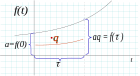
\includegraphics[width=9cm]{allg/funktionen/img/exp/exponentielles_wachstum.png} &
  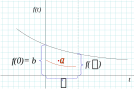
\includegraphics[width=7cm]{allg/funktionen/img/exp/exponentieller_zerfall.png}\\
\end{tabular}

%%\bbwCenterGraphic{10cm}{allg/funktionen/img/exp/exponentieller_zerfall.png}
%%\bbwCenterGraphic{11cm}{allg/funktionen/img/exp/exponentielles_wachstum.png}

Dabei sind
\begin{itemize}
\item $b=f(0)$ der Anfangsbestand zum Zeitpunkt $t$ = 0.
\item $\tau$ ist die typische Zeitspanne zwischen zwei Beobachtungszeitpunkten (zum Beispiel zwischen Wert und dessen Verdopplung). Beispiele:
  \begin{itemize}
  \item Verdoppeln in 3 Stunden: $a=2$ und $\tau = 3\, \text{h}$
    ($\text{h}$ = Stunden)
  \item Verfünf"|fachen einer Viertelstunde (= 15 Minuten): $a=5$ und
    $\tau=\frac{1}{4}\, \text{h}$
  \end{itemize}
  Meist ist die Beobachtungszeit gleichzeitig die Maßeinheit (\zB
  Veränderung pro Stunde). Dann ist unser $\tau=1$ und die Formel
  vereinfacht sich zu $f(t) = b\cdot{}a^t$.
\item $a$ ist der Zunahmefaktor zwischen zwei Beobachtungszeitpunkten (Beispiel $a=2$ bei Verdoppelungsprozessen).
  $a$ berechnet sich durch den Quotienten zwischen zwei
  Beobachtungswerten $a = \frac{f(\tau)}{f(0)} =\frac{m}{b}$.
\item
  Dabei ist $m$ der Messwert zum Zeitpunkt $\tau$.
\item $f(t)=b\cdot{}a^{\frac{t}{\tau}}$ ist der Wert (Anzahl, Fläche,
  Bestand, ...) zum Zeitpunkt
  $t$. 
\end{itemize}

Bemerkung: 
\TNTeop{
$\frac{m}b = \frac{f(\tau)}{f(0)}=\frac{b\cdot{}a^{\frac{\tau}{\tau}}}{b\cdot{}a^{\frac0{\tau}}}
  = \frac{a^1}{a^0} = \frac{a}{1} 
  = a$}%% END TNT
\newpage

\subsection{Referenzaufgabe}\index{Irland!Bevölkerungswachstum}
Irland hatte 1990 3.51 Mio. Einwohner. Im Jahr 2019 waren es bereits 4.93 Mio.

\textbf{Frage 1}: Was prognostizieren Sie für das Jahr 2025, wenn Sie von einem exponentiellen Wachstum ausgehen?

\noTRAINER{\bbwCenterGraphic{12cm}{allg/funktionen/img/exp/IrlandLeer.png}}%%

\TNTeop{
  Skizze:
  \bbwCenterGraphic{12cm}{allg/funktionen/img/exp/IrlandVoll.png}

  $\tau$ = 29 Jahre, Einheit = Jahre ($t$ in Jahren gemessen).
  
  $b=f(0) = 3.51$ [Mio EW] = Startwert (Taschenrechner STO).

  $m=f(\tau) = 4.93$ [Mio EW] = Messwert nach $\tau$ Jahren.

  $a=\frac{m}{b}=\frac{4.93}{3.51} \approx 1.4046$ pro 29 Jahre (Taschenrechner! STO). 

  $$f(t) = b\cdot{}a^\frac{t}{\tau}=b\cdot{}a^\frac{t}{29}$$


  TR Probe $b\cdot{}a^\frac{0}{29} = ? = 3.51$ 

  TR Probe $b\cdot{}a^\frac{29}{29} = ? = 4.93$ 

  Jahr 2025: $t=35$:

    $$f(35) = b\cdot{}a^\frac{35}{29}\approx 5.28899$$

}%% END TNT
\newpage

\subsection*{Aufgaben}

\GESO{\olatLinkArbeitsblatt{Exponentialfunktionen}{https://olat.bms-w.ch/auth/RepositoryEntry/6029794/CourseNode/106029175831971}{Kap. 1.5: Aufg. 18. a) b)}}
\TALS{\olatLinkArbeitsblatt{Exponentialfunktionen}{https://olat.bms-w.ch/auth/RepositoryEntry/6029786/CourseNode/106029175777725}{Kap. 1.5:     Aufg. 18. a) b) }}

\newpage

\textbf{Frage 2}: In wie vielen Jahren hat sich die Bevölkerung verdreifacht?

\TNTeop{
  Gesucht $T_3$ = Verdreifachungszeitpunkt.

  $$f(T_3) = 3\cdot{}f(0)$$

  Funktionsgleichung einsetzen:

  $$b\cdot{}a^\frac{T_3}{\tau} = 3\cdot{} b\cdot{} a^\frac0\tau$$

  Weil $a^{\frac{0}{\tau}} = 1$ folgt:

  $$b\cdot{}a^\frac{T_3}{\tau} = 3\cdot{} b$$

  $$a^\frac{T_3}{\tau} = 3$$

  Def. Logarithmus:

  $$\frac{T_3}{\tau} = \log_a(3)$$

$$T_3 = \tau\cdot{}\log_a(3) = 29\cdot{}\log_a(3) \approx 93.8$$
Die Bevölkerung wird sich voraussichtlich alle 94 Jahren
verdreifachen.

}%% END Trainer
\newpage

\subsection*{Aufgaben}
%%\TALSAadBMTA{221ff}{831 - 839}


\GESO{\olatLinkArbeitsblatt{Exponentialfunktionen}{https://olat.bms-w.ch/auth/RepositoryEntry/6029794/CourseNode/106029175831971}{Kap. 1.5:
    Aufg. 18. c), 19. - 21.}}
\TALS{\olatLinkArbeitsblatt{Exponentialfunktionen}{https://olat.bms-w.ch/auth/RepositoryEntry/6029786/CourseNode/106029175777725}{Kap. 1.5:
    Aufg. 18. c), 19. - 21. }}

\AadBMTA{338}{28. Bakterien}
\AadBMTA{352ff}{2. (Hasenpopulation), 7., 1. (optional)}
\olatLinkGESOKompendium{3.4}{27ff}{32., 34., 38., 40., 44., 45. und 46.}
\GESO{\aufgabenFarbe{Nullserie 2: Aufgabe 8.}}
\GESO{\aufgabenFarbe{Maturaprüfung 2017, Aufg. 12 (Raupen)\\
Maturaprüfung 2018 (Serie 3), Aufg. 11 (Müll)
}}



%% TODO Arbeitsblatt verlinken
%%\GESO{\olatLinkArbeitsblatt{Exponentialfunktionen}{https://olat.bms-w.ch/auth/RepositoryEntry/6029794/CourseNode/106029175831971}{Kap. 1.1: Voraussetzungen}}
%%\TALS{\olatLinkArbeitsblatt{Exponentialfunktionen}{https://olat.bms-w.ch/auth/RepositoryEntry/6029786/CourseNode/106029175777725}{Kap. 1.1: Voraussetzungen}}



\newpage

\subsection{Rate vs. Faktor
  II}\index{Rate}\index{Fatkor}\index{Zunahmefaktor}\index{Zunahmerate}
\totalref{RateZins1}

Den Unterschied von Zinsfuß (= Rate) und Zinsfaktor kennen wir bereits aus der Zinsrechnung.

So entspricht eine Zunahme von 12\% einem\\
Aufzinsungsfaktor von \LoesungsRaumLang{1.12}.

Wenn jedoch eine Beobachtung einer Zunahme von, sagen wir, 70\% innerhalb einer Viertelstunde beobachtet wird, so können wir uns fragen, um wie viel die Zunahme (als Rate oder Faktor) pro Zeiteinheit (hier Stunden) ist.


Füllen Sie dazu folgende Tabelle aus. Dabei bedeuten

\begin{tabular}{lp{14cm}}\hline
  Einheit & Stunden, Minuten, Meter, ... \\\hline
  $\tau$  & In dieser Zeitspanne (Stunden, Meter, ...) wird beobachtet \\\hline
  $p$     & Zunahme\textbf{rate}\index{Zunahmerate}\index{Rate} während $\tau$ Einheiten in \%. Ist $p$ negativ, handelt es sich um eine Abnahme\\\hline
  $a_\tau$ & Zunahme\textbf{faktor}\index{Zunahmefaktor} während $\tau$ Einheiten. Ist $a<1$, handelt es sich um einen Abnahmefaktor\\\hline
  $a_E$ (Formel)   & Zunahme pro Einheit (als Faktor). Aufgeschrieben als Formel\\\hline
  $\approx a_E$ (Zahl)  & Zunahme pro Einheit (als Näherungswert).\\\hline
  $p_E$   & Prozentuale Zunahme pro Zeiteinheit\\\hline
  \end{tabular} 

\leserluft{}
\leserluft{}
%% temporäres Platzhalterchen 
\newcommand{\ph}[1]{\noTRAINER{...........}\TRAINER{#1}}

%%\renewcommand{\arraystretch}{1.7}
$$f(t) = a_\tau^{\frac{t}\tau} = a_E^t$$
%% probably turn off auto-fill-mode in emacs when editing long lines
\begin{bbwFillInTabular}{|l|l|l|l|l|l|l|}\hline
  Einheit & $\tau$            &  $p$         & $a_\tau$         & $a_E$ (Formel)           &  $\approx a_E$    &$p_E$            \\\hline\hline
  h       &  $3$              &  56\%        & $1.56$           & $1.56^\frac13$            &  1.1598           & 11.598\%        \\\hline 
  h       &  $\frac14 = 0.25$ &  70\%        & \ph{1.7}         & \ph{ $1.7^\frac1{0.25}$}  &  \ph{8.3521}      & \ph{735.21\%}   \\\hline 
  h       &  $\frac12$        &  \ph{50\%}   & 1.5              &  $1.5^\frac1{0.5}$        &  2.25             & \ph{125\%}      \\\hline 
  Tage    &  $5$              & 100\%        & \ph{2}           & \ph{$2^\frac1{5}$}        &  \ph{1.1487}      & \ph{14.87}\%    \\\hline 
  Min.    &  $2$              & \ph{-60}\%   & 0.4              & \ph{$0.4^\frac1{2}$}      &  \ph{0.6325}      & \ph{-36.75}\%   \\\hline 
  m       &  $12$             & \ph{4.5}\%   & \ph{1.045}       & $1.045^\frac1{12}$        &  \ph{1.00367}     & \ph{0.3675}\%   \\\hline
  Wochen  & \ph{$2$}          & \ph{$200$}\% & \ph{3}           & $3^\frac12$               & \ph{1.73205}      & \ph{73.205}\%   \\\hline
  Jahr    & \ph{$\frac1{12}$} & \ph{$1$}\%   & \ph{$1.01$}      & $1.01^{\frac1{1/12}}$      &  \ph{$1.127$}     & \ph{$12.7$}\%   \\\hline
\end{bbwFillInTabular} 


\newpage

\subsection{Halbwertszeit, Verdopplungszeit}\index{Halbwertszeit}\index{Verdopplungszeit}

\begin{definition}{Halbwertszeit}{}
Die Zeitspanne, in der sich eine Menge halbiert, nennen wir
\textbf{Halbwertszeit} und bezeichnen diese Zeit mit:

$$T_{1/2}$$
\end{definition}

Die Halbwertszeit wird insbesondere
  beim radioaktiven Zerfall verwendet: nach wie viel tausend Jahren strahlt
  ein Stoff nur noch die Hälfte.


Beispiel: Ein Stoff nimmt innerhalb von sieben Tagen auf 80\% ab. Wie
groß ist seine Halbwertszeit $T_{1/2}$?

\TNTeop{
  Ansatz: $f(t) = b\cdot{}a^{\frac{t}{\tau}}$.

  $80\%$ und $7$ Tage einsetzen:

  $$f(t) = b\cdot{} 0.8^{\frac{t}{7}}$$

  Halber Wert:
  
  $$\frac{b}2= b\cdot{} 0.8^\frac{T_{1/2}}{7}$$
  $$\frac12  = 0.8^\frac{T_{1/2}}{7}$$

  Solver (num-solv): 21.74 (Tage) ...

 ... oder mit der Definition des Logarithmus:
  
  $$\frac{T_{1/2}}7 = \log_{0.8}\left(\frac12\right)$$
  $$T_{1/2} = 7\cdot{} \log_{0.8}\left(\frac12\right) \approx 21.74$$


  Bemerkung: $$f(t) =b\cdot{}0.8^\frac{t}7 \approx b\cdot{}\left(\frac12\right)^\frac{t}{21.74}$$
}%% END TNT
\newpage

\begin{gesetz}{Stoffmenge}{}
  Ist die Halbwertszeit $T_{1/2}$ und die anfängliche Stoffmenge $b$
  bekannt, so kann die Soffmenge zu jedem Zeitpunkt $t$ mit der
  folgenden Funktion $f$ angegeben werden:
  $$f(t) = \LoesungsRaumLen{50mm}{b\cdot{}\left(\frac12\right)^\frac{t}{T_{1/2}}}$$
\end{gesetz}
  
\begin{gesetz}{Halbwertzszeit}{}
  Die Halbwertszeit $T_{1/2}$ berechnet sich wie folgt:
  $$T_{1/2} = \LoesungsRaumLen{70mm}{\log_A\left(\frac12\right) = \tau
  \cdot{} \log_a\left(\frac12\right)}$$
  Dabei ist $A$ der Abnahmefaktor pro Zeiteinheit; $a$ während $\tau$ Zeiteinheiten.
\end{gesetz}


Herleitung:

\TNTeop{
  $$\frac12 \cdot{} f(0) = f(T_{1/2})$$
  $$\frac12 \cdot{} b    = b\cdot{}A^{T_{1/2}}$$
  $$\frac12 = A^{T_{1/2}}$$
  $$\log_A \left(\frac12\right) = T_{1/2}$$
}

\newpage
\GESO{Optional:}

\subsection{Verdopplungszeit}\index{Verdopplungszeit}

Analog gilt das Gesetz zur Verdopplung (s. obiges Beispiel Bevölkerung Irlands):
\begin{gesetz}{Verdopplungszeit}{}
  $$T_2 = \LoesungsRaumLen{40mm}{\log_A(2) = \tau \cdot{} \log_a(2)}$$

  $A$: der Abnahmefaktor pro Zeiteinheit; $a$ während $\tau$ Zeiteinheiten.
  
\end{gesetz}


\subsection*{Aufgaben}

\GESO{\olatLinkArbeitsblatt{Exponentialfunktionen}{https://olat.bms-w.ch/auth/RepositoryEntry/6029794/CourseNode/106029175831971}{Kap. 1.6:
    Halbwertszeit/Verdopplungszeit: Aufg. 22. - 25.}}
\TALS{\olatLinkArbeitsblatt{Exponentialfunktionen}{https://olat.bms-w.ch/auth/RepositoryEntry/6029786/CourseNode/106029175777725}{Kap. 1.6:
    Halbwertszeit/Verdopplungszeit: Aufg. 22. - 25.}}

\AadBMTA{352ff}{3. (Taucherin), 4. [Glasfaser ohne Teilaufgabe
    Eindringtiefe 4. b)] und 5. b) (radioaktiver Zerfall)}

\olatLinkGESOKompendium{3.4}{28ff}{42., 43. und 47.}

\GESO{\aufgabenFarbe{
    Maturaprüfung 2020, Aufg 11 (Käfer)\\
    Maturaprüfung 2018 (Serie 4), Aufg 10 (Cäsium 137)\\
    Maturaprüfung 2018 (Serie 2), Aufg 11 (Plutonium)\\
    Maturaprüfung 2018 (Serie 1), Aufg 11 (radioaktive Substanz)\\
    Maturaprüfung 2016, Aufg. 9 (Jod-131)
}}

\olatLinkGESOKompendium{3.4}{27ff}{32. bis 47.}

\newpage
\newpage
\section{Sättigungsprozesse, beschränktes Wachstum}
\sectuntertitel{Ich kann nicht mehr...}

\subsection*{Lernziele}
\begin{itemize}
	\item Grundformel eines Sättigungsfunktion
  \item Funktionsterm bei gegebenen Randbedingungen 
\end{itemize}

Bei beschränktem Wachstum ist die Änderungsrate typischerweise
proportional zur
sog. \textbf{Sättigungsdifferenz}\index{Sättigungsdifferenz}\index{Differenz!zur
  Sättigung}
(auch Sättigungs\textbf{manko}\index{Sättigungsmanko}\index{Manko!der
  Sättigung} oder Sättigungsdefizit\index{Sättigungsdefizit}).
  So bezeichnet man die \textbf{Differenz} zwischen dem
  aktuellen Wert und der Sättigungsgreze.

Mit anderen Worten: Je weiter weg der aktuelle Wert vom Grenzwert ist, umso rascher ist die Zunahme (bzw. die Abnahme bei beschränktem Zerfall).

\newpage


\subsection{Beispiele von Sättigungsprozessen}
Überlegen Sie sich Beispiele von Prozessen, bei welchen eine bestimmte Schwelle nicht überschreiten bzw. unterschritten werden kann:
\begin{itemize}
	\item \Lueckentext{Laden einer Batterie (je weniger geladen, um so schneller lädt sie)}
	\item \Lueckentext{Druck ablassen aus einem Pneu (je mehr Druck, umso schneller entweicht er)}
	\item \Lueckentext{Abkühlen eines Getränks bis zur Zimmertemperatur}
	\item \Lueckentext{Aufwärmen eines Getränks auf 40 Grad Celsius}
	\item \Lueckentext{Wirkstoffniveau bei Einnahme von Medikamenten.}
	\item \Lueckentext{Populationszunahme bei beschränkten Ressourcen (Futter, Platz, ...)}
        \item \Lueckentext{Lernkurve}
        \item \Lueckentext{\dotfill}
\end{itemize}
\newpage


\subsection{Begrenzter Zerfall}\index{Begrenzter Zerfall}\index{Zerfall!begrenzter}

\subsubsection{Einstiegsbeispiel Tee}\index{Tee!Abkühlungsprozess}\index{Abkühlungsprozess}

Tee wird von 75 Grad Celsius auf Zimmertemperatur (20 Grad)
abgekühlt. Nach drei Minuten messen wir 61 Grad.


a) Skizzieren Sie die «Zerfallskurve», welche die Temperatur des Tees
angibt.

b) Geben Sie die Funktionsgleichung $f(t)$ an, welche den Prozess
beschreibt.

c) Wann ist die Temperatur auf angenehme 37 Grad gesunken?


\TNTeop{1. Idee mit gleicher Formel klappt nicht, denn der
  Standard-Exponentielle Zerfall geht nach Null!

  Skizze mit 75 Grad, 20 Grad (Sättigung) und 51 Grad.

2. Idee: verschiebe die Skala um 20 Einheiten nach unten. Nun
funktioniert es: $g(t) = 55\cdot{}\left(\frac{41}{55}\right)^{\frac{t}{3}}$

3. Verschiebe wieder zurück: ACHTUNG: Das $b$ ist nun jedoch die
Sättigungs\textbf{differenz} zum Zeitpunkt $t_0=0$ und \textbf{nicht} mehr der Startwert! 

$$f(t) = 20 + g(t) = 20 + 55\cdot{}\left(\frac{41}{55}\right)^{\frac{t}{3}}$$

4. Berechnung: Wann sind 37 Grad erreicht? Einsetzen
in die Funktionsgleichung:

$$37\degre = y=f(t) = 20 + 55\cdot{}\left(\frac{41}{55}\right)^{\frac{t}{3}}$$

$$17=55\cdot\left(\frac{41}{55}\right)^\frac{t}{3}$$

$$\frac{17}{55}=\left(\frac{41}{55}\right)^\frac{t}{3}$$

$$\frac{t}3 = \log_{\left(\frac{41}{55}\right)}\left(\frac{17}{55}\right)$$


$$t=3\cdot{}\log_{\left(\frac{41}{55}\right)}\left(\frac{17}{55}\right)\approx
11.99 \textrm{ min.}$$

}%% END TNT

\newpage

\subsubsection{Allgemeine Form des beschränkten Zerfalls}
\begin{center}
\raisebox{-1cm}{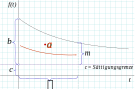
\includegraphics[width=13cm]{allg/funktionen/img/saettigung/saettigungskurveDown.png}}
\end{center}

Die Grundform eines begrenzten Zerfalls ist ein normaler
exponentieller Zerfall ($y=a^{t}$, $0<a<1$), der in $y$-Richtung um eine Sättigungsgrenze $c$ verschoben ist:

\begin{definition}{beschränkter Zerfall}{}
$$f(t) = c + b\cdot{}a^{\frac{t}{\tau}}$$
\end{definition}

Dabei ist:
\begin{itemize}
  \item $c+b = f(0) = y$-Achsenabschnitt = Startwert
	\item $c$: Die Sättigungsgrenze\index{Sättigungsgrenze} (Sättigungswert). Dies ist die Annäherungskonstante oder der \textbf{Asymtote}nwert\index{Asymptote}: Tiefer kann die Funktion nicht fallen.

	\item $m$:
    Sättigungs\textbf{differenz}\index{Sättigungsdifferenz}\index{Differenz!zur
      Sättigung}. Wie viel fehlt, bis zur
    Sättigungsgrenze: $m = f(t) - c$. Die Sättigungs\textbf{differenz} nimmt exponentiell ab.
	\item $b$: Die \textbf{Abweichung} zu $c$ zum Zeitpunkt $t=0$. Der
    Anfangswert ist somit $f(0) = c + b$; mit anderen Worten: $b$ ist das
    \textbf{Sättigungsdifferenz} zum Zeitpunkt $t_0 = 0$.

    \item $a=\frac{m}{b}=\frac{f(\tau)-c}{f(0)-c}$: Der Faktor der Veränderung der
      Sättigung\textbf{differenz}.
\end{itemize}

\subsection*{Aufgaben}
\GESOAadBMTA{359}{35. (Kuchen) und 36. (Ovomaltine)}
\olatLinkGESOKompendium{3.4.2}{33}{48. (Achtung: Das
  Kompendium verwendet andere Buchstaben: Das dortige $a$ ist unser $b$.)}

\GESO{\olatLinkArbeitsblatt{Exponentialfunktionen}{https://olat.bbw.ch/auth/RepositoryEntry/572162163/CourseNode/106029175831971}{Kap. 3.1:
    Sättigung: Begrenzter Zerfall}}
\TALS{\olatLinkArbeitsblatt{Exponentialfunktionen}{https://olat.bbw.ch/auth/RepositoryEntry/572162090/CourseNode/106029175777725}{Kap. 3.:
    Sättigung: Begrenzter Zerfall}}
\newpage


\subsection{Sättigung (begrenztes Wachstum)}\index{Sättigung}\index{begrenztes Wachstum}\index{Wachstum!begrenztes}
\subsubsection{Einstiegsbeispiel 1: Eistee wärmen}
Das Aufwärmen von Eistee von $5\degre$ Kühlschranktemperatur auf $20\degre$ Zimmertemperatur ist ein klassisches «Begrenztes Wachstum» (mit gespiegelter Exponentialfunktion).

\TNT{5.2}{Skizze}

\subsubsection{Einstiegsbeispiel 2: Batterie laden}
\begin{center}
\raisebox{-1cm}{
\includegraphics[width=8cm]{allg/funktionen/img/saettigung/batterien.png}}
\end{center}

Eine 9V-Batterie ist etwas mehr als zur Hälfte entladen und enthält nun eine
Restspannung von 4V.

Wenn wir 9V an die Batterie anlegen, so wird die Batterie geladen.

Die Batterie lädt sich umso rascher, je \textit{leerer} sie ist.

Die Batterie lädt sich umso langsamer, je \textit{voller} sie ist.


\newpage

\subsubsection{Allgemeine Form von Sättigungsprozessen}

\begin{center}
\raisebox{-1cm}{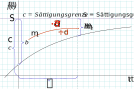
\includegraphics[width=13cm]{allg/funktionen/img/saettigung/saettigungskurve.png}}
\end{center}

Die Grundform des begrenzten Wachstums ist ein exponentieller Zerfall\totalref{zerfallsfunktion},
der an der $x$-Achse gespiegelt und in $y$-Richtung
verschoben ist:

\begin{definition}{Sättigung}{}
$$f(t) =c - b\cdot{} a^{\frac{t}{\tau}}$$
\end{definition}

Die Variable haben die folgenden Bedeutungen:

\begin{itemize}
	\item $c$: Sättigungsgrenze. Dies ist die Annäherungskonstante oder der Asymtotenwert. Höher kann die Funktion nicht steigen.

	\item $m$ ist die
    Sättigungsdifferenz\index{Sättigungsdifferenz}\index{Differenz!zur
    Sättigung}. Wie viel fehlt, bis zur
    Sättigungsgrenze: $m = c - f(t)$. Auch hier nimmt die Sättigungs\textbf{differenz} exponentiell ab.
	\item $b$: Die Abweichung des Funktionsgraphen zu $S$ zum Zeitpunkt $t=0$. Der
    Anfangswert ist somit $f(0) = c - b$.
\item $a=\frac{m}{b}=\frac{c-f(\tau)}{c-f(0)}$ Faktor der Veränderung
  der Sättigungs\textbf{differenz}.
\end{itemize}


\subsubsection{Bemerkungen}
\begin{bemerkung}{}{}
  Für die Sättigungsdifferenz gilt:

\TNT{4}{$$m = m(t) = c - f(t) = c - \left(c-b\cdot{}a^{\frac{t}{\tau}}\right) = + b\cdot{}a^{\frac{t}{\tau}}$$

und somit:

$$m_0 = m(0) = b\cdot{}a^0 = b$$}%% END TNT
\end{bemerkung}

\TRAINER{ Bemerkung (Trainer/mündlich):
  
Das $a$ kann aus zwei \textbf{beliebigen} Sättigungsdifferenz-Werten berechnet werden (die um die
Zeitdifferenz $\tau$ auseinander liegen):
$$\frac{m_2}{m_1} = \frac{b\cdot{}a^{\frac{t_2}{\tau}}}{b\cdot{}
  a^{\frac{t_1}{\tau}}} = a^{\frac{t_2}{\tau}} : a^{\frac{t_1}{\tau}} =
a^{\frac{t_2-t_1}{\tau}} = a^{\frac{\tau}{\tau}} = a$$%% 
}%% END Trainer


\begin{bemerkung}{}{}
Meistens ist $m_0$ zum Zeitpunkt $t=0$ bekannt und somit ist $b=m_0$. Es reicht, die Messung zum Zeitpunkt $t_0$ und zu einem weiteren Zeitpunkt durchzuführen. Wenn zusätzlich die Sättigungsgrenze $c$ bekannt ist, kann die Funktion $f$ komplett bestimmt werden.
\end{bemerkung} 

\newpage

\subsection{Referenzaufgaben}

\subsubsection{Berechnung am Batterie-Beispiel}\index{Batterie}
Eine Batterie weist zum Zeitpunkt $t_0$ vier Volt auf. Nach sechs Stunden am Ladegerät zeigt die Messung sieben Volt. Wir wissen, dass die Sättigungsgrenze (Ladespannung) bei neun Volt liegt.

Zeichnen Sie die gegebenen Größen in ein Koordinatensystem ein und markieren Sie bei neun Volt eine horizontale Beschränkungslinie (\zB 1V = 1 Häus'chen in $y$-Richtung; 1h = 1 Häus'chen in $x$-Richtung).

\noTRAINER{\mmPapier{8.8}}
\TRAINER{\bbwCenterGraphic{15cm}{allg/funktionen/img/saettigung/batterieFct.png}}

\textbf{Frage 1}: Wie lautet die Formel $f(t) = ...$ der Sättigungskurve?

\noTRAINER{$c = ..........................$}
\TRAINER{$c = \textrm{ Sättigungsgrenze } = 9 [\textrm{V}]$}

\noTRAINER{$b = ..........................$}
\TRAINER{$b = m_0 = c-f(0) = 9 - 4 = 5$}

\noTRAINER{$m =  ..........................$}
\TRAINER{$m = m_1 = c-f(\tau) = 9 - 7 = 2$}

\noTRAINER{$a = .........................$}
\TRAINER{$a=\frac{m}{b} = \frac{m_1}{m_0} = \frac{2}{5} = 0.4$}

\noTRAINER{$\tau = .........................$}
\TRAINER{$\tau = 6$ ($e_x$ = eine Stunde)}


\noTRAINER{$f(t) = c - b\cdot{}a^{\frac{t}{\tau}} = ..... - .....\cdot{}(.....)^{\frac{-t}{.....}}$}
\TRAINER{$f(t) = c - b\cdot{}a^{\frac{t}{\tau}} = 9 - 5\cdot{}(\frac{2}{5})^{\frac{t}{6}}$}

\TRAINER{Die Kontrollen für $t=0$ und $t=6$ sind mit dem Stehenlassen von $a$ als Bruch nun sehr einfach.}
\newpage

\textbf{Frage 2}: Wann wird die Batterie zu 99\% geladen sein?

\TNTeop{99\% von 9V = 8.91 V

  Somit ist $t$ gesucht mit $f(t) = 9 - 5\cdot{}\left(\frac25\right)^{\frac{t}{6}} = 8.91$

  (beidseitig -9 und Vorzeichen drehen und dann durch 5 teilen, so folgt...)

  $$(0.4)^{\frac{t}{6}} = (9-8.91) : 5 = 0.09 : 5 = 0.018$$

  Definition Logarithmus:

  $$\frac{t}6 = \log_{0.4}(0.018) \approx 26.3 $$

  Nach ca. 26 - 27 Stunden ist die Batterie zu 99\% geladen.
}
\newpage

\subsubsection{Referenzaufgabe Sättigung: Pneu}\index{Reifen}\index{Pneu}

Ein Reifen (Pneu) ist anfänglich ganz leer und enthält «nur» 1 atm, nämlich den
Druck der Umgebung. (1 atm = atmosphärischer Druck = technische Atmosphäre) 

Der Reifen wird aufgepumpt mit einer Druckpumpe, die maximal 2 atm
leisten
kann. Mit 2 atm ist hier gemeint: 2 at mehr als der
Umgebungsdruck. Somit könnte der Pneu bis auf maximal 3 atm aufgepumpt
werden (= Sättigungsgrenze).

Um den Reifen optimal zu füllen, wird er auf 2 atm aufgepumpt (1 atm
über dem Umgebungsluftdruck).

Die Pumpe schafft in den ersten 10 Sekunden den Druck von 1 atm auf 1.2
atm (= 0.2 atm über Normaldruck) aufzupumpen.

Nach wie vielen Sekunden muss gestoppt werden, damit der Reifen
optimal gepumpt ist?

\TNTeop{Die Sättigungsdifferenz schwindet von $m_1=3-1=2$ bis $m_2=3-1.2=1.8$
innerhalb der ersten $10s = \tau$. Die Sättigungsgrenze liegt bei
$S=3$. Unsere (Exponential)basis $a$ ist somit $1.8 / 2$, was uns
liefert:
$$f(t) = 3 - 2\cdot{}\left(\frac{1.8}{2}\right)^\frac{t}{10}$$
Somit ist das Optimum bei $2 = 3-
2\cdot{}\left(\frac{1.8}{2}\right)^\frac{t}{10}$ erreicht, also bei
etwa 65.8 Sekunden.
}
\newpage

\GESO{\subsection*{Aufgaben}}
\GESOAadBMTA{358}{34. (Eistee)}
\olatLinkGESOKompendium{3.4.2}{32ff}{49. - 51. (Bem.: Das
  Kompendium gibt die Funktionsterme bereits an und verwendet als
  Basis i.\,d.\,R. die Eulersche Konstante $e\approx{} 2.71828$)}

\GESO{\olatLinkArbeitsblatt{Exponentialfunktionen}{https://olat.bbw.ch/auth/RepositoryEntry/572162163/CourseNode/106029175831971}{Kap. 3.1:
    Begrenztes Wachstum}}%% END GESO
\TALS{\olatLinkArbeitsblatt{Exponentialfunktionen}{https://olat.bbw.ch/auth/RepositoryEntry/572162090/CourseNode/106029175777725}{Kap. 3.1:
    Begrenztes Wachstum}}%% END TALS

\newpage

\subsection{Zusammenfassung der Prozesse}
\vspace{8mm}
\begin{center}\textbf{Wachstum und Zerfall}\end{center}

\TNT{8.8}{\bbwCenterGraphic{18cm}{allg/funktionen/img/zusammenfassung_exp/wachstum_zerfall.png}

  bzw.
  $$f(t) = G_0 \cdot{} \e^{qt}; q=  \frac{\ln(a)}\tau  \,\,\,\,\,\,\,\,\, f(t) = G_0 \cdot{} \e^{-qt}; q  = \frac{-\ln(a)}\tau$$
}%% END TNT

\vspace{8mm}
\begin{center}\textbf{Sättigung}\end{center}

\TNTeop{\bbwCenterGraphic{18cm}{allg/funktionen/img/zusammenfassung_exp/saettigung.png}

    bzw.
     $$f(t) = S + (G_0-S) \cdot{} \e^{q\cdot{}t}; q=    \frac{\ln(a)}\tau     \,\,\,\,\,\,\,\,\, f(t) = S + (S - G_0) \cdot{} \e^{-q\cdot{}t}; q  = \frac{-\ln(a)}\tau$$

Hier ist Platz für das Video/die Videos zur den getanzten
Funktionen (S. OLAT/Wiki).
}%% END TNTeop

\newpage

\TALS{
  \subsection*{Aufgaben}
  \olatLinkTALSStrukturaufgabenSPF{Basiskenntnisse Funktionen Teil
    1}{5}{4., 5., 8. und 9.}
  \olatLinkTALSStrukturaufgabenSPF{Basiskenntnisse Funktionen Teil
    2}{14}{45., 47. und 49.}
}%% END TALS
\newpage


%%%%%%%%%%%%%%%%
% Funktionen I
%%%%%%%%%%%%%%%55
%% Funktionen II GESO Metapackage
\part{Funktionen II}\index{Funktionen!II|textbf}
\renewcommand{\bbwPartID}{FCT2}
\section{Potenzfunktionen}\index{Funktion!Potenzfunktionen}\index{Potenzfunktionen}
\sectuntertitel{Funktionen hoch drei!}

\subsection*{Lernziele}

\begin{itemize}
\item Definition Ganzzahlige Potenzfunktion
\item Graphische Darstellung
\end{itemize}
\newpage


\subsection{Einstieg}

%%%%%%%%%%%%%%%%%%%%%%%%%%%%%%%%%%%%%%%%%%%%%%%%%%%%%%%%%%%%%%%%%
\subsubsection{Beispiel: Rationale Funktion\GESO{ (optional)}}

Betrachten wir einmal die Funktion $f: y = 0.1x^3 + x^2 + 2x + 3 - x^{-1}$ \zB mit Geogebra (\texttt{www.geogebra.org}).

\bbwGraph{-10}{4}{-7}{8}{%
  \bbwFunc{0.1*\x*\x*\x + \x*\x + 2*\x + 3 -1/\x}{-8.5:-0.2}
  \bbwFunc{0.1*\x*\x*\x + \x*\x + 2*\x + 3 -1/\x}{0.1:1.5}
}%%


Polynomfunktionen und rationale Funktionen sind «\textit{weiche}» Funktionen, die jedoch \textbf{Asymptoten}\index{Asymptote} (hier bei $x=0$) aufweisen können.
Ebenso sind die Extremwerte (lokale Maxima und Minima)\TALS{ wie auch die Wendepunkte} charakteristische Stellen und oft Gegenstand der Untersuchung.
Wir beschränken uns \TALS{vorerst }auf Funktionen der Art $f: y=a\cdot{}x^z$
mit $z \in \mathbb{Z}\backslash\{0\}$\TRAINER{ $z=0$ ist eine
  Proportionalität und somit hier unspannend}.

\newpage



\subsubsection{\GESO{Beispiel}\TALS{Repetition}: Reinquadratische Funktion}\index{quadratische Funktion}\index{Funktion!quadratische}

Zeichnen Sie den Graphen der Funktion $f: y= \frac16 x^2$:

\bbwGraph{-7}{7}{-1}{6.5}{%%
  \TRAINER{
    \bbwFunc{\x*\x/6}{-6:6}
  }
}%%

\begin{definition}{Reinquadratische Funktion}{}
Die Funktion

$f: y = a\cdot{}x^2$

heißt \textbf{Parabel zweiter Ordnung} oder rein-quadratische Funktion.
\end{definition}


\TALS{
\begin{bemerkung}{}{}
Eine allgemeine quadratische Funktion besitzt auch noch einen linearen ($bx$) und einen konstanten ($c$) Anteil. Die allgemeine quadratische Funktion hat die Form

$$f: y= ax^2 + bx + c$$
\end{bemerkung}
}%% END TALS

\TALS{Beispiele zu allgemeinen quadratischen Funktionen finden sie im
  Buch \cite{marthaler21alg} ab Seite 260 insb. im Bild zu Aufg. 4 auf
  Seite 273.}%% END TALS

\newpage

\subsection{Parabel}\index{Parabel}

Zeichnen Sie $y = \frac{1}{16}x^4$ im Bereich $[-3; 3]$ indem Sie für jeden 0.5-er $x$-Wert das zugehörige $y$ berechnen:

\bbwGraph{-4}{4}{-1}{6.5}{%%
  \TRAINER{\bbwFunc{\x*\x*\x*\x/16}{-3:3}}
}%%


\begin{definition}{Parabel}{definition_parabel}
  Ist $n\in \mathbb{N}_{\ge 2}$, so wird der Graph der Potenzfunktion
  $$x\mapsto a\cdot{}x^n$$
  \textbf{Parabel} $n$-ter Ordnung genannt.
\end{definition}

\TALS{%%
\begin{bemerkung}{Potenzfunktion}{definition_potenzfunktion}
  Eine Funktion der Art
$$f: y=a\cdot{}x^r$$
  mit $r \in \mathbb{R}\backslash\{0\}$ heißt \textbf{Potenzfunktion}.
\end{bemerkung}

\begin{bemerkung}{Polynomfunktionen}{}
  Funktionen, deren Funktionsterm ein Polynom bilden werden
  \textbf{Polynomfunktionen} genannt:
  $$f: y=a_n\cdot{}x^n + a_{n-1}\cdot{}x^{n-1} + a_{n-2}\cdot{}x^{n-2} + ... + a_2\cdot{}x^2 + a_1 \cdot{} x + a_0 $$
\end{bemerkung}
%
}%% END TALS


\newpage
\subsection*{Aufgaben}
\aufgabenFarbe{Zeichnen Sie die Parabeln $$y=f(x) = x^n$$ für $n = 2$,
  $n=3$, $n=4$, $n=5$ und $n=6$ mit \texttt{geogebra.org}.
\\
Was fällt auf?}
%%\GESOAadBMTA{303ff}{1. (nur $n=3$ und $n=5$), 2. (nur $n=4$ und $n=6$)}

\TNTeop{}

\newpage

\subsubsection{Anwendung (optional)}
Boltzmannsches T-hoch-vier-Gesetz\index{Boltzmann!$T^4$-Gesetz}

\leserluft{}

Die Funktion $P(T) = \sigma\cdot\varepsilon\cdot
  A\cdot{}T^4$ beschreibt, welche Strahlungsleistung $P$ ein Körper der
  Oberfläche $A$ (in $ \text{m}^2$) bei Temperatur $T$ (in Kelvin) aussendet.

  $\sigma$ = Bolzmann Konstante = $5.6\cdot{}10^{-8}$
  
  $\varepsilon$ = Emissionswert

  \small{\texttt{(eg. https://ennologic.com/wp-content/uploads/2018/07/Ultimate-Emissivity-Table.pdf)}}

  \leserluft{}
  
  Rechenbeispiel:

\TNTeop{$T$ = 20 Grad Zimmertemperatur in Kelvin: 293.15;
  Brick (Haus) hat Emissionswert ca. 0.75; Haus Oberfläche $500 \text{m}^2$

  $$P(293.15) \approx 5.6\cdot{}10^{-8} \cdot{} 0.75 \cdot{} 500
  \cdot{} 293.15^4 \approx 155 \text{kW} $$
  Natürlich strahlt eine 20-grädige Umgebungstemperatur gleich viel
  wieder zurück, sodass keine 'Heizkosten' entstehen.

  Heizen wir das Haus nun zwei Grad wärmer, so erhalten wir:
  $$P(295.15) \approx 5.6\cdot{}10^{-8} \cdot{} 0.75 \cdot{} 500
  \cdot{} 295.15^4 \approx 159.4 \text{kW} $$

  Dies entspricht einer Differenz von 4.28 kW für nur zwei Grad wärmer
  im Haus!
  

}%% END TNT
\newpage

Zeichnen Sie des weiteren die Funktion $y = \frac{1}{9}x^3$:

\bbwGraph{-4}{4}{-5}{5}{%%
  \TRAINER{\bbwFunc{\x*\x*\x/9}{-3.5:3.5}}
}%%

\subsubsection{Symmetrien}\index{Symmetrien!von Parabeln}\index{Parabel!Symmetrie}
Was fällt für gerade und ungerade Exponenten auf? Gibt es Spiegelachsen
oder Spiegelpunkte?

\renewcommand{\mmPapier}[1]{\mmPapierZwei{#1}{16.4}}
\begin{tabular}{c|p{8cm}}
  $x^2$ & \vspace{0.1mm}\TNT{0.8}{An der $y$-Achse}\\\hline
  $x^3$ & \vspace{0.1mm}\TNT{0.8}{Am Ursprung $O(0|0)$}\\\hline
  $x^4$ & \vspace{0.1mm}\TNT{0.8}{wie $x^2$}\\\hline
  $x^5$ & \vspace{0.1mm}\TNT{0.8}{wie $x^3$}\\\hline
\end{tabular}
\renewcommand{\mmPapier}[1]{\mmPapierZwei{#1}{17.6}}


\GESO{Eine Zusammenfassung der wichtigsten Eigenschaften von
  Potenzfunktionen finden Sie im Buch \cite{marthaler21alg} Seite 296 oben.}
\newpage

\subsubsection{Referenzaufgabe}

Bestimmen Sie $a$ und $k$ so, dass der Graph von $y = a \cdot{} x^k$
durch die Punkte $P=\left(3 \middle| 1458\right)$ und
$Q=\left(-4\middle|8192\right)$ verläuft.

\TNT{15.2}{ Punkte einsetzen in die Funktionsgleichung:
  \gleichungZZ{1458}{a\cdot{}3^k}{8192}{a\cdot{}(-4)^k}
  Aus der oberen Gleichung das $a$ ermitteln ($a=\frac{1458}{3^k}$)
  (I) und in die zweite
  Gleichung einsetzen: $$8192 = \frac{1458}{3^k} \cdot{} (-4) ^k$$
  Exponent $k$ separieren:
  $$\frac{8192}{1458} = \left(\frac{-4}3\right)^k$$
  Problem: Logarithmen mit negativen Basen (hier $\frac{-4}3$)
  funktionieren nicht!
  
  Weil nun $k$ gerade sein muss, folgt dass $\left(\frac{-4}3\right)^k
  = \left(\frac43\right)^k$. Daraus ergibt sich
  $$\frac{8192}{1458} = \left(\frac{4}3\right)^k \Longrightarrow k =
  \log_{\frac43}\left(\frac{8192}{1458}\right) = 6$$
  Dieses $k$ nun in die Gleichung (I) einsetzen; dies
  liefert
  $$a=\frac{1458}{3^k} = 2.$$
}%% end TRAINER


\subsection*{Aufgaben}
\AadBMTA{305ff}{11. a) b) c), 13. a) c), (optional 17.,)  18.}
%%\TALSAadBMTA{197}{735. (6) (7) und (9) jeweils mit geogebra, 736. a) d),
%%  737. a) c), 739.}
\newpage


\subsection{Translationen}\index{Manipulation!Funktionen}\index{Funktions-Manipulation}\index{Translation!Funktion}
\sectuntertitel{Manipulation an Funktionsgraphen}
(Verschiebung\index{Verschiebung}, Spiegelung\index{Spiegelung},
Streckung\index{Streckung})

\TadBMTA{217}{13.3}
%%\TALSTadBFWA{163}{3}
Betrachten Sie die Funktionen

$$f(x) = a\cdot{}\left(\frac{x\TALS{-d}}b\right)^5\TALS{+c}$$
und
$$g(x) = a\cdot{}\left(\frac{x\TALS{-d}}b\right)^4\TALS{+c}$$

mit Geogebra (\texttt{geogebra.org})
und beschreiben Sie die Effekte der Parameter

$a$: \TRAINER{Streckung in $y$-Richtung. $a$ negativ: Spiegelung an der
$x$-Achse.}

\noTRAINER{\mmPapier{2.4}}

$b$: \TRAINER{Streckung entlang der $x$-Achse. $b$ negativ: Spiegelung
  an der $y$-Achse.}

\noTRAINER{\mmPapier{2.4}}

\TALS{%% nur TALS haben Verschiebungen
  $c$: \TRAINER{Verschiebung entlang der $y$-Achse}

\mmPapier{2.4}
}%% end TALS

\TALS{
$d$: \TRAINER{Verschiebung entlang der $x$-Achse (Verschiebung nach
  rechts verlangt ein negatives $d$.)}

\noTRAINER{  \mmPapier{2.4}}
}%% END TALS

\newpage

\subsubsection{Zusammenfassung der Translationen}


Wir betrachten die verschiedenen geometrischen
Funktions-«Manipulationen» (Abbildungen) am Beispiel {\color{red}$y =f(x) = \frac18 x^3$}.


\newcommand{\graphTranslationMultiColumn}[5]{%
  \multicolumn{3}{|l|}{#1}\\%%
\hline%%
\graphTranslationMultiColumnZ{#2}{#3}{#4}{#5}
}%% end new command \graphTranslationMultiColumn

\newcommand{\graphTranslationMultiColumnZ}[4]{%
\multirow{5}{6cm}{#1} &  & \multirow{2}{*}{\begin{minipage}{.3\textwidth}\raisebox{-8cm}{\includegraphics[width=\linewidth,height=60mm]{allg/funktionen/img/translation/#4}}\end{minipage}}\\[55mm]%%
&\fbox{#2}&\\%%
&&\\%%
&{\color{red}\fbox{#3}}&\\%%
&&\\%%
\hline%%
}%% end new command \graphTranslationMultiColumnZ

\TALS{%% Nur TALS haben Verschiebungen
\begin{tabular}{|p{7cm}|c|c|}%%
\hline%%
\graphTranslationMultiColumn{Verschiebung in $y$-Richtung...}{... um \textbf{zwei} Einheiten nach \textbf{oben}:}{$g(x)=f(x)\textbf{+2}$}{$g(x)=\frac18x^3\textbf{+2}$}{typ1.png}
\graphTranslationMultiColumnZ{... um \textbf{eine} Einheiten nach \textbf{unten}:}{$g(x)=f(x)\textbf{-1}$}{$g(x)=\frac18x^3\textbf{-1}$}{typ2.png}
\end{tabular}%%
}%% end TALS

\begin{tabular}{|p{7cm}|c|c|}%%
\hline%%
\graphTranslationMultiColumn{Spiegelung...}{... an der $x$-Achse:}{$g(x)=-f(x)$}{$g(x)=-\frac18x^3$}{typ3.png}
\graphTranslationMultiColumnZ{... an der $y$-Achse:}{$g(x)=f(-x)$}{$g(x)=\frac18(-x)^3$}{typ4.png}
\end{tabular}%%

\begin{tabular}{|p{7cm}|c|c|}%%
\hline%%
\graphTranslationMultiColumn{Streckung...}{... in $y$-Richtung (von der $x$-Achse aus) um Faktor \textbf{zwei}:}{$g(x)=\textbf{2}\cdot{}f(x)$}{$g(x)=\textbf{2}\cdot{}\frac18x^3$}{typ5.png}
\graphTranslationMultiColumnZ{... in $x$-Richtung (von der $y$-Achse aus) um Faktor \textbf{zwei}:}{$g(x)=f(\frac{1}{\textbf{2}}\cdot{}x)$}{$g(x)=\frac18(\frac{1}{\textbf{2}}\cdot{}x)^3$}{typ6.png}
\end{tabular}%%

\TALS{%% Nur TALS verschieben in x-Richtung
\begin{tabular}{|p{7cm}|c|c|}%%
\hline%%
\graphTranslationMultiColumn{Verschiebung in $x$-Richtung\footnote{Kein prüfungsrelevantes Thema.}...}{... um \textbf{zwei} Einheiten nach \textbf{links}:}{$g(x)=f(x\textbf{+2})$}{$g(x)=\frac18(x\textbf{+2})^3$}{typ7.png}
\graphTranslationMultiColumnZ{... um \textbf{zwei} Einheiten nach \textbf{rechts}:}{$g(x)=f(x\textbf{-2})$}{$g(x)=\frac18(x\textbf{-2})^3$}{typ8.png}
\end{tabular}%%
}%% END TALS
\newpage

\subsection*{Aufgaben}
\GESO{
Skizzieren Sie $-\frac{1}{2}x^3 - 1$ im Bereich $x$ = -2 bis $x$ = +2.

\bbwGraph{-4}{4}{-5}{3}{%%
  \TRAINER{%
    \bbwFunc{-0.5*\x*\x*\x-1}{-2:2}%
  }%%
}%

Vergleichen Sie die neue Funktion mit der Parabel $y=x^3$.

\TNT{5.2}{Die neue Funktion ist an der $y$-Achse gespiegelt, ist um
  50\% gestaucht ($y$-Richtung) und ist um eine Einheit nach unten
  ($x$-Richtung) verschoben worden.}
}%% END GESO

\AadBMTA{304ff}{5. a) c) d) e), 9. a) d) e)}

 
\TALS{
  \aufgabenFarbe{Zeichnen Sie mit \texttt{geogebra.org} die Funktion
    $f(x) = \frac1{10}(x^3 - 3x^2 + 3)$
    \\
    Definieren Sie anschließend die Funktion $$g(x) = a\cdot{}f((x+s)\cdot{}b)+r.$$
\\
    Entscheiden Sie, welche Veränderungen die Parameter $a$, $b$, $r$
    und $s$ bewirken.\\
    Starten Sie mit $a=1$, $b=1$, $r=0$ und $s=0$.
  }%% END Aufgabenfarbe
  \TNT{4}{
    $r$: Verschiebung nach oben\\
    $s$: Verschiebung nach links\\
    $a$: Streckung in $y$-Richtung\\
    $b$: Stauchung in $x$-Richtung
  }%% END TNT
}%% END TALS



%%  OLAT Arbeitsblatt
\GESO{\olatLinkArbeitsblatt{Positive Potenzfunktionen zuordnen}{https://olat.bbw.ch/auth/RepositoryEntry/572162163/CourseNode/104752086007823}{(alle Beispiele)}}%% END olatLinkArbeitsblatt
\TALS{\olatLinkArbeitsblatt{Positive Potenzfunktionen zuordnen}{https://olat.bbw.ch/auth/RepositoryEntry/572162090/CourseNode/105597875231723}{(alle Beispiele)}}%% END olatLinkArbeitsblatt


\olatLinkTALSStrukturaufgabenSPF{Teil 2}{15ff}{48. und 51.}
%%\TALS{\aufgabenFarbe{Strukturaufgaben SPF Teil 2: Taschenrechner: S. 15ff:  Aufg. 48. und 51.}%% END Aufgabenfarbe
%%}%% END TALS

%%\TALSAadBMTA{197 ff.}{739., 743. c), 745. c), 738.*}

\olatLinkGESOKompendium{3.3.1.}{26}{28., 29.}
\newpage



%%%%%%%%%%%%%%%%%%%%%%%%%%%%%%%%%%%%%%%%%%%%%%%%%%%%%%%%%%%%%%%%%%%%%%%%%%%%%%%%%%%
\subsection{Hyperbel}\index{Hyperbel (negative Exponenten)}

(«Hyperbel» Griechisch = «über das Ziel hinaus werfen»)


Zur Erinnerung:
\begin{multicols}{2}
\begin{itemize}
	\item $x^{-1} = \frac{1}{x}$
	\item $x^{-2} = \frac{1}{x^2}$
	\item $x^{-3} = \frac{1}{x^3}$
	\item $x^{-4} = \frac{1}{x^4}$
	\item $x^{-5} = \frac{1}{x^5}$
  \item ...
\end{itemize}
\end{multicols}

Zeichnen Sie die Funktion $f: y = x^{-1}$ im Definitinosbereich
$\DefinitionsMenge{} = [-5;5]\TRAINER{\backslash \{0\}}\noTRAINER{......}$

\bbwGraph{-6}{6}{-3}{3}{%%
  \TRAINER{\bbwFunc{1/\x}{-5:-0.3}}
  \TRAINER{\bbwFunc{1/\x}{0.3:5}}

}%%

\newpage


Zeichnen Sie zusätzlich Funktion $f: y = x^{-2}$ im Definitionsbereich $[-5;5]$:

\bbwGraph{-6}{6}{-5}{5}{%%
  % x^-2
  \TRAINER{\bbwFuncC{1/(\x * \x)}{-5:-0.447}{green}}%% 0.447 = 1/sqrt (5)
  \TRAINER{\bbwFuncC{1/(\x * \x)}{0.447:5}{green}}
  \TRAINER{\bbwLetter{2.5,0.5}{x^{-2}}{green}}
  \TRAINER{\bbwLetter{-1.5,1}{x^{-2}}{green}}

  %x^-3
%  \TRAINER{\bbwFuncC{1/(\x * \x * \x)}{-5:-0.584}{blue}}
%  \TRAINER{\bbwFuncC{1/(\x * \x * \x)}{0.584:5}{blue}}
%  \TRAINER{\bbwLetter{0.8,0.3}{x^{-3}}{blue}}
%  \TRAINER{\bbwLetter{-1.2,-3.8}{x^{-3}}{blue}}
%  \TRAINER{\bbwLetter{1.2,4.5}{x^{-3}}{blue}}

}%%

\begin{definition}{Hyperbel}{definition_hyperbel}
  Der Graph einer Potenzfunktion $$f: y=ax^z$$
  mit $z \in \{-1, -2, -3, -4, ...\}$ heißt
\textbf{Hyperbel}\index{Hyperbel} der Ordnung $z$.
\end{definition}

Der Definitionsbereich von Hyperbeln entspricht dem Definitionsbereich
des Funktionsterms. Merke: Es darf nicht durch Null geteilt werden:

$$x^{-5} = \frac{1}{x^5} \Longrightarrow \DefinitionsMenge{} = \mathbb{R} \backslash \{0\}$$


\subsection*{Aufgaben}
\AadBMTA{306ff}{19. Zeichnung mit geogebra.org, 20.
  Zeichnung mit geogebra.org}
%%\TALSAadBMTA{205}{771. a) c) d) e) g) h) j)}


\newpage

\subsubsection{Charakteristiken}
\textbf{Spiegelungen:}\\

Welche Funktionen $x$, $x^{-1}$, $x^{-2}$, $x^{-3}$ sind an welchen Achsen bzw. Punkten gespiegelt?

\renewcommand{\mmPapier}[1]{\mmPapierZwei{#1}{16.0}}
\begin{tabular}{c|p{10cm}}
  $x^{-1}$ &  \TNT{0.8}{Am Ursprung $O(0|0)$ : Punktspiegelung}\\
  \hline
  $x^{-2}$ &  \TNT{0.8}{An der $y$-Achse: Achsensymmetrie}\\
  \hline
  $x^{-3}$ &  \TNT{0.8}{Am Ursprung $O(0|0)$: Punktspiegelung}\\
  \hline
  $x^{-4}$ &  \TNT{0.8}{An der $y$-Achse: Achsensymmetrie}\\
  \hline  
\end{tabular}
\renewcommand{\mmPapier}[1]{\mmPapierZwei{#1}{17.6}}


\paragraph{Definitions- und Wertebereiche:}

Geben Sie für die obigen Funktionen an, was ihr Definitions- bzw. Wertebereich ist\footnote{Grundmenge ist $\mathbb{R}$.}:

\begin{tabular}{c|c|c}
Funktionsterm & Definitionsbereich $\DefinitionsMenge{}$& Wertebereich $\Wertebereich{}$\\ \hline
  $x^{-1}$ & \TRAINER{$\mathbb{R}\backslash\{0\}$} &  \TRAINER{$\mathbb{R}\backslash\{0\}$}\\ \hline
  $x^{-2}$ & \TRAINER{$\mathbb{R}\backslash\{0\}$} &  \TRAINER{$\mathbb{R}^{+}\backslash\{0\}$}\\ \hline
  $x^{-3}$ & \TRAINER{$\mathbb{R}\backslash\{0\}$} &  \TRAINER{$\mathbb{R}\backslash\{0\}$}\\ \hline
  $x^{-4}$ & \TRAINER{$\mathbb{R}\backslash\{0\}$} &  \TRAINER{$\mathbb{R}^{+}\backslash\{0\}$}\\ \hline
\end{tabular}


\GESO{\subsection*{Aufgaben}}
\olatLinkGESOKompendium{3.3}{26}{28. bis 31.}
\GESO{\aufgabenFarbe{Aufgabe der Nullserie 2 (zweite Nullserie): Aufg. 7 auf Seite 3}}
\GESO{\aufgabenFarbe{Maturaprüfung 2016, Aufg. 8 (Graphen zuordnen)}}

\newpage

\newpage

%%%%%%%%%%%%%%%%%%%%%%%%%%%%%%%%%%%%%%%%%%%%%%%%%%%%%%%%%%%%%%%%%%%%%%%%%%%%%%%%%%%

\subsection{Zusammenfassungen und Überblick}\index{Potenzfunktionen!Überblick}

$$y = a\cdot{}x^z$$

$z$ gerade: Gespiegelt an der $y$-Achse

$z$ ungerade: Gespiegelt am Ursprung $O=(0|0)$

Ist ${\color{ForestGreen}a>0}$\TRAINER{ (grün in der Graphik)}, so sind Graphen mit
geraden Exponenten nach oben geöffnet bzw. mit ungeraden Exponenten im
Quadranten I und III.

Ist ${\color{red}a<0}$\TRAINER{ (rot/orange in der Graphik)}, so sind Graphen mit
geraden Exponenten nach unten geöffnet bzw. mit ungeraden Exponenten
im Quadranten II und IV.


\TRAINER{%
  \includegraphics[width=8.5cm]{allg/funktionen/img/potenzfct/potenzFunktionenGerade.png}\hfill{}\includegraphics[width=8.5cm]{allg/funktionen/img/potenzfct/potenzFunktionenUngerade.png}
}%% END Trainer
\noTRAINER{%
  \includegraphics[width=8.5cm]{allg/funktionen/img/potenzfct/potenzFunktionenLeer.png}\hfill{}\includegraphics[width=8.5cm]{allg/funktionen/img/potenzfct/potenzFunktionenLeer.png}
}%% END Trainer


\subsection*{Aufgaben}
\AadBMTA{307}{25. b) c), 26. a)\TALS{ b)}, 27. b) c)\TALS{, 33*}}

\newpage


\newpage
\newpage
%%
%% 2019 07 04 Ph. G. Freimann
%%

\section{Exponentialfunktionen}\index{Funktion!Exponentialfunktion}\index{Exponentialfunktionen}
\sectuntertitel{Go viral!}
%%%%%%%%%%%%%%%%%%%%%%%%%%%%%%%%%%%%%%%%%%%%%%%%%%%%%%%%%%%%%%%%%%%%%%%%%%%%%%%%%
\subsection*{Lernziele}

\begin{itemize}
\item Definition Exponentialfunktion
\item Koeffizienten interpretieren
\item Graph: Symmetrien, Polstellen, Asymptoten, Schnittpunkte mit
  Achsen
  \item Basiswechsel
\end{itemize}

\TadBMTA{322}{19}
%%\TALS{(\cite{frommenwiler17alg} S.215 (Kap. 3.10))}
%%\GESO{(\cite{marthaler21alg}       S.322 (Kap. 19))}
\newpage

\subsection{Aussehen von Exponetialfunktionen}


Zeichnen Sie $f: y=2^x$ und $g: y=1.4^x$ ins selbe Koordinatensystem:


\bbwGraph{-5}{5}{-1}{5}{
\TRAINER{  \bbwFuncC{pow(2.0,\x)}{-3.5:2.1}{blue}
  \bbwFuncC{pow(1.4,\x)}{-3.5:3}{green}
  \bbwLetter{1,3}{$f$}{blue}
  \bbwLetter{2.5,2}{$g$}{green}
}%% end TRAINER
}%% end graph

\begin{definition}{Exponentialfunktion}{}\index{Exponentialfunktionen!Definition}
  Eine Funktion der Form $$f(x): x \mapsto a^x$$
  bzw. $$y = a^x$$
  mit $a\in \mathbb{R}^{+}\backslash\{1\}$ heißt \textbf{Exponentialfunktion}.
\end{definition}


\begin{bemerkung}{Zunahmefaktor}{}\index{Zunahmefaktor|textbf}
Der Parameter $a$ gibt den Wachstumsfaktor pro Zeiteinheit $e_x$ an.
\end{bemerkung}


\subsubsection*{Aufgaben}
\GESO{\olatLinkArbeitsblatt{Exponentialfunktionen}{https://olat.bms-w.ch/auth/RepositoryEntry/6029794/CourseNode/106029175831971}{Kap. 1.2:
    Einfache Wachstumsprozesse: Aufgaben 4. bis 6.}}
\TALS{\olatLinkArbeitsblatt{Exponentialfunktionen}{https://olat.bms-w.ch/auth/RepositoryEntry/6029786/CourseNode/106029175777725}{Kap. 1.2:
    Einfache Wachstumsprozesse: Aufgaben 4. bis 6.}}

\newpage

\subsection{Formen der Darstellung}
Zeichnen Sie die Funktionen $f: y=2^x$, $g: y=2^{-x}$ und $h: y=\left(\frac12\right)^x$ in dasselbe Koordinatensystem:

\bbwGraph{-6}{6}{-1}{5}{
  \TRAINER{\bbwFuncC{exp(0.69314718*\x)}{-6:2}{blue}}
  \TRAINER{\bbwFuncC{exp(-0.69314718*\x)}{-2:6}{red} }
  \TRAINER{\bbwLetter{1.5,4}{2^x}{blue}}
  \TRAINER{\bbwLetter{-5,4}{g(x)=2^{-x}=\left(\frac{1}{2}\right)^x=h(x)}{red}}
}

Bemerkung: \TRAINER{$$2^{-x} = \frac1{2^x} = \frac{1^x}{2^x}= \left(\frac12\right)^x$$}
\newpage



\subsubsection{Umkehrung (Optional)}
Um aus einem Wachstum einen Zerfall zu modellieren können wir entweder
die Zeitachse umdrehen oder den Kehrwert der Basis verwenden.
umgedreht werden:

Mit $d := \frac1a $ gilt:

\begin{center}
  \fbox{$a^{+t} = \left(\frac1a\right)^{-t} = d^{-t} $}
\end{center}

\newpage

\newpage

\subsection{Verschiebung und Streckung \GESO{(optional)}}

Eine Verschiebung der Exponentialfunktion $y=b\cdot{}a^x$ in der Zeit ($x$-Richtung) kann auch in Form einer Veränderung der Startfaktors $b$ umgeschrieben werden.

Verschieben wir \zB $$y=2^x$$ um fünf Einheiten nach rechts, so liest sich die neue Funktionsgleichung wie folgt:
$$y=2^{x-5}.$$

(Zeichnen Sie in \texttt{geogebra.org} a) $y=2^x$ und b) $y=2^{x-5}$.)

Dies kann jedoch auch umgeschrieben werden:

$$2^{x-5} = 2^x \cdot{} 2^{-5} = 2^{-5} \cdot{} 2^x = \frac{1}{2^5} \cdot{} 2^x =
\frac{1}{32}\cdot{}2^x$$

\bbwCenterGraphic{8cm}{allg/funktionen/img/exp/verschiebung_gleich_streckung.png}
Bildlegende: Eine Verschiebung ($x$-Richtung) der Exponentialfunktion entspricht einer Stauchung ($y$-Richtung) der selben Exponentialfunktion.

\TALS{Es gilt hier $$a^{x-b}=\frac{a^x}{k}$$ mit
$k=a^b$ und mit $b=\log_a(k)$.}

\newpage


\subsection{Punkte einsetzen\GESO{ (optional)}}
Wie bei den linearen Funktionen oder bei den Potenzfunktionen können auch Exponentialfunktionen gefunden werden, wenn bereits Punkte auf dem Graphen bekannt sind:

\textbf{Referenzaufgabe}

Finden Sie die Parameter $a$ und $b$ der Exponentialfunktion
$$f: y=b\cdot{}a^x$$
wenn Sie wissen, dass die Funktion durch die Punkte $P=(2|4)$ und $Q=(-1|2)$ verläuft:

\TNTeop{
  In Gleichung einsetzen:

  \gleichungZZ{4}{b\cdot{}a^2}{2}{b\cdot{}a^{-1}}

  Einsetzverfahren: Zum Beispiel aus der zweiten Gleichung das $b$ ermitteln...
  $$b = 2 a (III)$$
  ... und in die erste Gleichung einsetzen:

$$4 = 2a\cdot{} a^2$$
  $$2 = a^3$$
  $$a=\sqrt[3]{2}$$
  In (III) einsetzen:

  $$b = 2 \sqrt[3]{2}$$

  Ergo: $$f(x) = b\cdot{}a^x = 2\cdot{}\sqrt[3]{2} \cdot{} \left(\sqrt[3]2\right)^x \approx 2.5198 \cdot{} 1.2599^x$$
}

\subsection*{Aufgaben}
%%\AadBMTA{334}{10. a) b)\TALS{ e)}\GESO{ f)}}
\GESO{\olatLinkArbeitsblatt{Exponentialfunktionen}{https://olat.bms-w.ch/auth/RepositoryEntry/6029794/CourseNode/106029175831971}{Kap. 2.1: E-Funktion / Punkte-Aufgaben Aufg 26. a) b) ($e^{qt}$ optional) und Aufg. 27.}}
\TALS{\olatLinkArbeitsblatt{Exponentialfunktionen}{https://olat.bms-w.ch/auth/RepositoryEntry/6029786/CourseNode/106029175777725}{Kap. 2.1: E-Funktion / Punkte-Aufgaben Aufg 26. a) b) ($e^{qt}$ optional) und Aufg. 27.}}

\AadBMTA{336}{23. d}

\newpage

\newpage
%% 2019 07 04 Ph. G. Freimann
%%

\section{Wachstum und Zerfall}\index{Wachstum}\index{Zerfall}
\sectuntertitel{Sagt ein großer Stift zum kleinen Stift: ``Wachsmalstift!''}

%%%%%%%%%%%%%%%%%%%%%%%%%%%%%%%%%%%%%%%%%%%%%%%%%%%%%%%%%%%%%%%%%%%%%%%%%%%%%%%%%

\TRAINER{
  Video \href{https://www.youtube.com/watch?v=TMaLuks8dxw}{MatheMann}
Wo schneiden sich $x^3$ und $e^x$?}%%
\subsection*{Lernziele}

\begin{itemize}
\item Zinseszins
\item Wachstums-, Zerfallsprozesse
\item Verdoppelungs- und Halbwertszeiten
%%\item Basiswechsel
\end{itemize}

\TadBMTA{342}{20}
%%\TALS{(\cite{frommenwiler17alg} S.221 (Kap. Exponentielles Wachstum))}
%%\TALS{(\cite{frommenwiler17alg} S.223 (Kap. Exponentielle Abnahme))}
%%\TALS{(\cite{frommenwiler17alg} S.225 (Kap. Zinseszins))}
%%\GESO{(\cite{marthaler21alg}       S.342 (Kap. 20))}

\newpage


\subsection{Beispiele}
Bei Wachstumsprozessen sprechen wir dann von einer exponentiellen
Zunahme, wenn die Zunahme pro Zeiteinheit immer proportional zum aktuellen Bestand ist.

\begin{itemize}
\item \Lueckentext{Zinseszins}
\item \Lueckentext{Frequenzen in der temperierten Stimmung
  (Musik). Zunahme der Frequenz pro Halbtonschritt.}
\item \Lueckentext{Keime in der Kuhmilch; Ansteckungsbedingte Krankheitsfälle (\zB viral)}
\item \Lueckentext{Algenbefall in Teichen}
\item \Lueckentext{Generell Populationen: Flechten, Pilze}
\item \Lueckentext{(ungebremstes) Bevölkerungswachstum / bzw. Tierpopulation}
\item \Lueckentext{\dotfill}
\end{itemize}


\GESO{\olatLinkArbeitsblatt{Exponentialfunktionen}{https://olat.bms-w.ch/auth/RepositoryEntry/6029794/CourseNode/106029175831971}{Kap. 1.1:
    Voraussetzungen: Aufgaben 1. bis 3.}}
\TALS{\olatLinkArbeitsblatt{Exponentialfunktionen}{https://olat.bms-w.ch/auth/RepositoryEntry/6029786/CourseNode/106029175777725}{Kap. 1.1:
    Voraussetzungen: Aufgaben 1. bis 3.}}


\newpage

\subsection{Einstiegsbeispiel Taschengeld}

Bei Familie Cash kann man aussuchen, wie sich sein Taschengeld über
die Jahre «vermehrt». Mani wählt Variante A. Bei Varante A erhält man
CHF 1.- im ersten Jahr, CHF 2.- im 2. Jahr, CHF 3.- im 3. Jahr und so
weiter bis zur abgeschlossenen Grundbildung im 13. Jahr CHF 13.-.

Carla wählt Variante B. Bei der Variante B erhält Carla auch CHF 1.-
im ersten Jahr, dann aber jedes Jahr 30\% mehr, als im Vorjahr.

a) Wird Carla vor Ende der Grundbildung jemals mehr als Mani erhalten?

\LoesungsRaumLang{Ja, im 10. Schuljahr}

b) Wer hat über alle Jahre mehr Taschengeld?

\LoesungsRaumLang{Carla wird mehr haben}

c) Skizzieren Sie beide Varianten:

\TRAINER{\bbwCenterGraphic{13cm}{allg/funktionen/img/taschengeldAusgefuellt.png}}
\noTRAINER{\bbwCenterGraphic{16cm}{allg/funktionen/img/taschengeld.png}}

\TRAINER{Optional: Zeige mit Geogebra (\texttt{geogebra.org}) $x^2$ vs. $1.2^x$. Fazit:
  Exponentielles Wachstum überholt jegliche Potenzfunktion.}



\newpage

Zeichnen Sie $f: y=2^x$ und $g: y=1.4^x$ ins selbe Koordinatensystem:


\bbwGraph{-5}{5}{-1}{5}{
\TRAINER{  \bbwFuncC{pow(2.0,\x)}{-3.5:2.1}{blue}
  \bbwFuncC{pow(1.4,\x)}{-3.5:3}{green}
  \bbwLetter{1,3}{$f$}{blue}
  \bbwLetter{2.5,2}{$g$}{green}
}%% end TRAINER
}%% end graph

\begin{definition}{Exponentialfunktion}{}\index{Exponentialfunktionen!Definition}
  Eine Funktion der Form $$f(x): x \mapsto a^x$$
  bzw. $$y = a^x$$
  mit $a\in \mathbb{R}^{+}\backslash\{1\}$ heißt \textbf{Exponentialfunktion}.
\end{definition}


\begin{bemerkung}{Wachstumsfaktor}{}\index{Wachstumsfaktor}
Der Parameter $a$ gibt den Wachstumsfaktor pro Zeiteinheit $e_x$ an.
\end{bemerkung}


\subsubsection*{Aufgaben}
\GESO{\olatLinkArbeitsblatt{Exponentialfunktionen}{https://olat.bms-w.ch/auth/RepositoryEntry/6029794/CourseNode/106029175831971}{Kap. 1.2:
    Einfache Wachstumsprozesse: Aufgaben 4. bis 6.}}
\TALS{\olatLinkArbeitsblatt{Exponentialfunktionen}{https://olat.bms-w.ch/auth/RepositoryEntry/6029786/CourseNode/106029175777725}{Kap. 1.2:
    Einfache Wachstumsprozesse: Aufgaben 4. bis 6.}}


\newpage

\subsection{Exponentieller Zerfall}\label{zerfallsfunktion}
Die Funktion $f(x): x \mapsto y = d^{-x}$ ist eine
Exponentialfunktion, die gegen Null geht.

\bbwFunction{-4}{4}{-1}{8}{exp(-\x)}{-2:4}

\begin{bemerkung}{}{}
Oft wird bei Wachstumsprozessen die Zeitachse auch mit $t$ statt $x$ bezeichnet: $t$ steht für \textit{time}.
\end{bemerkung}

\newpage

\subsubsection{Beispiele}
\begin{itemize}
	\item \Lueckentext{Zinsliche Abschreibungen (\zB Wert eines Autos)}
	\item \Lueckentext{Radioaktiver Zerfall}
	\item \Lueckentext{Lichtintensität in Medium (Gas / Flüssigkeit / Glasfaser), dies gilt vertikal, wie auch horizontal}
	\item \Lueckentext{Atmosphärischer Luftdruck in Metern über Meer}
  \item \Lueckentext{Entladen einer Batterie bzw. eines Kondensators}
  \item \Lueckentext{Sauerstoffkonzentration in Seen (\zB Herbst bei kontinuierlicher Abnahme)}
  \item \Lueckentext{Abnahme des Bierschaums im Glas}
  \item \Lueckentext{Mischen, wie im Sirup-Beispiel\totalref{sirup_beispiel}}
  \item \Lueckentext{«Halbwertszeit des Wissens» ;-)}
  \item \Lueckentext{\dotfill}
\end{itemize}

\newpage



Zeichnen Sie die Funktionen $f: y=2^x$, $g: y=2^{-x}$ und $h: y=\left(\frac12\right)^x$ in dasselbe Koordinatensystem:

\bbwGraph{-6}{6}{-1}{5}{
  \TRAINER{\bbwFuncC{exp(0.69314718*\x)}{-6:2}{blue}}
  \TRAINER{\bbwFuncC{exp(-0.69314718*\x)}{-2:6}{red} }
  \TRAINER{\bbwLetter{1.5,4}{2^x}{blue}}
  \TRAINER{\bbwLetter{-5,4}{g(x)=2^{-x}=\left(\frac{1}{2}\right)^x=h(x)}{red}}
}

Bemerkung: \TRAINER{$$2^{-x} = \frac1{2^x} = \frac{1^x}{2^x}= \left(\frac12\right)^x$$}
\newpage

\subsubsection{Grundform} \index{Exponentieller Prozess! Grundform}
Die Grundform für Zerfallsprozesse lautet:

\begin{definition}{Zerfall}{}\index{Zerfall}
  Die Grundform des exponentiellen Zerfalls wird beschrieben durch die Funktion
$$f(x): x \mapsto a^x$$
  bzw.
  $$y = a^x$$
\end{definition}


\begin{gesetz}{Wachstum vs. Zerfall}{}

  Der einzige Unterschied bei Wachstums- bzw Zerfallsprozessen ist der
  Faktor $a$:

  \begin{itemize}
    \item \LoesungsRaumLen{40mm}{$a>1$: Wachstum}\vspace{3mm}
    \item \LoesungsRaumLen{40mm}{$0<a<1$: Zerfall}
  \end{itemize}
  
\end{gesetz}

\begin{bemerkung}{$x$-Richtung}{}
  Exponentielle Prozesse laufen meist in der Zeit ab. Somit wird
  die $x$-Achse zur Zeitachse und meist mit $t$ (Time) bezeichnet:
  $$f(t) = a^t$$
  \end{bemerkung}


\subsubsection{Umkehrung (Optional)}
Um aus einem Wachstum einen Zerfall zu modellieren können wir entweder
die Zeitachse umdrehen oder den Kehrwert der Basis verwenden.
umgedreht werden:

Mit $d := \frac1a $ gilt:

\begin{center}
  \fbox{$a^{+t} = \left(\frac1a\right)^{-t} = d^{-t} $}
\end{center}

\newpage

\subsection*{Aufgaben}
%%\TALSAadBMTA{223ff}{840., 841., 843., 844. und 846.}

\GESO{\olatLinkArbeitsblatt{Exponentialfunktionen}{https://olat.bms-w.ch/auth/RepositoryEntry/6029794/CourseNode/106029175831971}{Kap. 1.3: Zerfall: Aufg. 7., 8. und 9.}}
\TALS{\olatLinkArbeitsblatt{Exponentialfunktionen}{https://olat.bms-w.ch/auth/RepositoryEntry/6029786/CourseNode/106029175777725}{Kap. 1.3: Zerfall: Aufg. 7. 8. und 9.}}

\AadBMTA{354}{9. (Bauchspeicheldrüse)}
\olatLinkGESOKompendium{3.4.1}{27ff}{33., 35., 36., 39. und 41.}

\newpage
%% Sirup-Beispiel
\subsection{Mischtank}\index{Mischtank}\index{Sirup}\label{sirup_beispiel}
Wird ein Glas Wasser in ein Glas Sirup geschüttet, so

\TRAINER{\bbwCenterGraphic{5cm}{allg/alg/potenzen_wurzeln/img/Schwapp.png}}%%
\noTRAINER{\bbwCenterGraphic{5cm}{allg/alg/potenzen_wurzeln/img/SchwappOhneFormel.png}}

geschieht erst mal etwas eher klebriges:
\begin{itemize}
  \item Das Wasser verdrängt den Sirup und
  \item das Sirupglas schwappt über.
\end{itemize}

Wenn man nun gleichzeitig im Sirupglas
umrührt, so mischt sich das Wasser mit dem Sirup und je länger man
Wasser einschüttet, umso verdünnter wird der Sirup.


Wie viel Sirup bleibt im Glas?

\TNT{2.4}{
Am Ende bleibt ein
Verhältnis von Wasser : Sirup = $\left(1-\frac{1}{e}\right) : \left(\frac{1}{e}\right)$
\vspace{1.5cm}
}

Diese Konstante wird oft in großen chemischen Mischtanks verwendet,
gibt aber auch ein Maß an, wenn \zB in einer Minergie-Wohnung die Luft
ausgetauscht wird. Wenn nämlich das Volumen der Wohnung einmal neu hineingepumpt (bzw. weggeblasen) wurde während sich alte die Luft im Haus permanent mit der neuen vermischt, so ist noch ein Anteil von \TRAINER{$\frac{1}{e}$}\noTRAINER{ ..... } der alten Luft im Haus.
\newpage


\textbf{Begründung:}\\
1. Gedanke: Jedes eingefüllte Glas, vermindert die vorhandene
Sirupkonzentration um den selben Faktor. Ergo handelt es sich um
einen exponentiellen Zerfall.

\leserluft

2. Gedanke: Wir tauschen drei Mal $\frac13$ aus. Nehmen also im
\begin{itemize}
\item \textbf{ersten Schritt} $\frac13$ des Sirups weg (und ersetzen diesen mit Wasser).
  Es bleiben $\frac23$ Sirup. Den Rest füllen wir mit Wasser auf.
\item Im \textbf{zweiten Schritt} nehmen wir $\frac13$ des Gemisches
weg; es verbleiben also $\frac23$ von $\frac23$ an
Sirup-Konzentrat. Der Rest wird immer wieder mit Wasser aufgefüllt. Mit
anderen Worten: Es bleiben $\frac23 \cdot \frac23
= \left(\frac23\right)^2$ an Sirup\footnote{Man könnte hier auch argumentieren mit: «Wir nehmen von den $\frac23$ einen Drittel weg»: $\frac23 - (\frac13$ von $\frac23)$ = $\frac23 - (\frac13 \cdot\frac23) = \frac23 \cdot(1-\frac13)=\frac23\cdot\frac23$}.
\item Im \textbf{dritten Schritt} entnehmen wir wieder $\frac13$ des
Gemisches; es verbleiben wieder $\frac23$ vom bisherigen Sirup, also
$\frac23$ von $(\frac23)^2$ also $\left(\frac23\right)^3$.

Beim dreistufigen Gedankenexperiment verbleiben
$\left(\frac23\right)^3 = \left(1-\frac13\right)^3$ der ursprünglichen Konzentration.
\end{itemize}
\leserluft

3. Gedanke: Das Experiment vom vorherigen Gedanken können wir natürlich auch mit immer kleineren\TALS{, sogenannten infinitesimalen,} Schritten durchführen.
Mit Centilitern \zB im dl-Glas ersetzen wir 10 Mal je $\frac1{10}$. 
So verbleibt am Schluss $\left(1-\frac{1}{10}\right)^{10}\approx 0.35$ Sirup.

\GESO{Wenn wir (\zB mit dem Taschenrechner) die Schrittanzahl immer weiter vergrößern (und somit die pro Schritt ausgetauschte Menge immer verkleinern), so ergibt sich für 1000 Schritte ein Verhältnis von $\left(1-\frac{1}{1000}\right)^{1000}\approx 0.3677 \approx \frac1{\e}$. }
\TALS{Wenn wir die Schritte permanent erhöhen (und gegen Unendlich gehen lassen), so erhalten wir den Grenzwert (lat. Limes) von

$$\lim_{n\rightarrow\infty} \left(1-\frac{1}{n}\right)^n = \frac1{\e}$$
}
\newpage

\textbf{Aufgabe 1: Sirup}\\
Wie viel Wasser muss eingeschüttet werden, damit das auf der Flasche
angegebene Verhältnis von 1:6 (1 Teil Sirup, 6 Teile Wasser) zustande
kommt?

\TNT{8}{
Bei 1x Schütten, erhalten wir $\left(\frac{1}{\e}\right)^1$ Anteil Sirup.

Bei 2x Schütten, erhalten wir $\left(\frac{1}{\e}\right)^2$ Anteil Sirup.

Somit erhalten wir den Siebtel (1:6 = $\frac17$-Anteil) indem wir die
folgende Exponentialgleichung lösen:

$$\frac17 = \left(\frac{1}{\e}\right)^n$$
Diese Gleichung lösen wir, indem wir beidseitig logarithmieren und so
erhalten wir den einzuschüttenden Teil $$n=\ln(7)\approx{1.946}.$$
}%% END TNT

\textbf{Aufgabe 2: Minerige-Haus}\\
Wenn wir also wissen wollen, wie viel Luft in ein Minergiehaus
eingepumpt werden muss, damit nur noch 1 Promille der alten Luft
vorhanden ist, so erhalten wir
\TNTeop{
  $$\text{Volumen Neuluft} = \text{Wohnungsvolumen}\cdot{}\ln(1000)$$
  $$\ln(10000) \approx 6.9$$
} %% end TNT


\newpage

\newpage


\subsection{Startwert}\index{Startwerte!bei Wachstums- und Zerfallsprozessen}

Die bisher betrachteten Exponentialfunktionen haben für den Wert $x=0$ (bzw. $t=0$) immer den
$y$-Wert = 1 bzw. 100\%.
Da in der Praxis meist konkrete Werte vorgegeben sind verwenden wir
eine \textbf{allgemeinere Form der Exponentialfunktion}.

\subsubsection{Einstiegsbeispiel}

\begin{beispiel}{Pilz}{}
  Ein Pilzbefall an einer Wand nehme täglich um 23\% der Fläche
  zu\footnote{Je nach Organismus ist auch ein quadratisches Wachstum
  vorhanden, doch für unser Experiment verwenden wir exponentielles Wachstum.}.
  Anfänglich wird eine Fläche von $35$ $\text{cm}^2$ gemessen.
  Welche Fläche ist nach einem, nach zwei, nach fünf, nach zehn
  bzw. nach $n$ 
  Tagen zu erwarten?

  \TNT{6}{Ein  Tag:   $35\cdot{} 1.23^1    =          43.05 \text{cm}^2$\\
          Zwei Tage:  $35\cdot{} 1.23^2   \approx{}  52.95 \text{cm}^2$\\
          Fünf Tage:  $35\cdot{} 1.23^5   \approx{}  98.54 \text{cm}^2$\\
          Zehn Tage:  $35\cdot{} 1.23^{10} \approx{} 277.4 \text{cm}^2$\\
          $n$  Tage:  $35\cdot{} 1.23^n = 35\cdot{}1.23^n$}%% END TNT

  Wann wird die ganze Wand ($6 \text{ m}^2$) mit dem Pilz befallen
  sein?
  
\TNT{6}{$6 \text{ m}^2 = 60\,000 \text{ cm}^2$
     
     ergo: $60\,000 = 35 \cdot{} 1.23^n$

     (durch 35 teilen, dann logarithmieren)

     $$\frac{60\,000}{35} = 1.23^n$$

     $$n = \log_{1.23}\left(\frac{60\,000}{35}\right) \approx 35.97 \text{Tage}$$

   }%% END TNT

\end{beispiel}

\newpage


\begin{gesetz}{Exponentialfunktion mit frei wählbarem Startwert}{}
$$f: y = \LoesungsRaumLen{40mm}{b\cdot{}a^x}$$

Auch hier gibt der Parameter $a$ den Wachstumsfaktor pro Zeiteinheit $e_x$ an.

Dabei ist $b$ der Startwert zum Zeitpunkt $x$ = 0.
\end{gesetz}


\noTRAINER{\bbwCenterGraphic{8cm}{allg/funktionen/img/exp/b_faktor.png}}
\TRAINER{\bbwCenterGraphic{8cm}{allg/funktionen/img/exp/b_faktor_trainer.png}}

\begin{bemerkung}{Wachstumsfaktor}{}{}
Werden zwei $x$ Positionen mit Differenz 1 (=$e_x$) betrachtet, so sind
die zugehörige $y$-Werte um \textbf{Faktor} $a$ auseinander.
\end{bemerkung}

Begründung:
\TNTeop{
  Gegeben $x_1$ und $x_2 = x_1 + 1$. So ist

  $y_1 = b\cdot{}a^{x_1}$ und $y_2 = b\cdot{}a^{x_2}$.

  Setzen wir nun $x_1 + 1$ für $x_2$ ein, so erhalten wir:

  $$y_2 = f(x_2) = b\cdot{}a^{x_2} = b\cdot{} a^{x_1+1} =  b\cdot{}a^{x_1} \cdot{} a^1 = y_1\cdotp{} a$$
}
\newpage


\subsection*{Aufgaben}

\GESO{\olatLinkArbeitsblatt{Exponentialfunktionen}{https://olat.bms-w.ch/auth/RepositoryEntry/6029794/CourseNode/106029175831971}{Kap. 1.4:
    Frei wählbarer Startwert: Aufg. 10. Gummiball; 11. Neophytenplage;
    12: Tierpopulation; 13. Licht im Wasser;  weitere Aufgaben 14. bis 17.}}
\TALS{\olatLinkArbeitsblatt{Exponentialfunktionen}{https://olat.bms-w.ch/auth/RepositoryEntry/6029786/CourseNode/106029175777725}{Kap. 1.4:
    Frei wählbarer Startwert: Aufg. 10. Gummiball; 13. Licht im Wasser. 14. Federpendel; 15. Luftdruck; weitere Aufgaben aus
    Kap. 1.4.}}
 
  \AadBMTA{338}{29. (Bierschaum)}
  \AadBMTA{353}{6. (C-14 Methode)}

  Als Vorbereitung zur allgemeinen Wachstumsfunktion:
  \AadBMTA{207}{10. (Algen)}

\newpage


\subsection{Beobachtungszeitspanne}
\subsubsection{Einstgiesbeispiel}
\bbwCenterGraphic{17cm}{allg/funktionen/img/tuerlersee2.jpg}
\begin{center}{\small Legende: Türlersee April 2022}\end{center}

Der Türlersee ist ein kleiner See im Reppischtal. Seine Oberfläche
begann sich vor einigen Jahrzehnten stark mit Algen\footnote{Genau
  genommen handelte es sich um Zooplanktonbiomasse zwischen 1982 und 1994, doch als
  Idee zur Exponentialfunktion sollte ein ungefähres Flächenmodell reichen.} zu bedecken.

Anfänglich (zum Zeitpunkt $t=0$) waren gerade mal 20$m^2$ bedeckt. Doch nach fünf Tagen hatte sich diese Fläche verdoppelt und nach weiteren fünf Tagen nochmals verdoppelt (also insgesamt vervierfacht).

Füllen Sie die (prognostizierte) Wertetabelle für 30 Tage ein:

\def\spaceX{\,\,\,\,\,\,\,\,\,\,}
\newcommand\tuerlerB[1]{\noTRAINER{\spaceX}\TRAINER{#1}}
\begin{tabular}{l|c|c|c|c|c|c|c}
  $t$:  & 0 & 5 & 10 & 15 & 20 & 25 & 30 \\
  \hline
  $m^2$ & \tuerlerB{20}  & \tuerlerB{40}  &   \tuerlerB{80}  &  \tuerlerB{160}  &  \tuerlerB{320}  &  \tuerlerB{640}  &  \tuerlerB{1280} \\
\end{tabular}

\newpage
Zeichnen Sie die Algenpopulation als Graph in eine Koordinatensystem
(beginnen Sie mit dem Ursprung ganz links unten. $x$-Achse in Tagen ($t$). $y$-Achse in $\text{m}^2$.

\noTRAINER{\bbwCenterGraphic{170mm}{allg/funktionen/img/exp/WachstumTuerlerseeLeer.png}}
\TRAINER{\bbwCenterGraphic{10cm}{allg/funktionen/img/exp/tuerlerAlgen.png}}
\newpage

\textbf{Funktionsgleichung}

Wir betrachten die selbe Algenpopulation mit einer
Ver\textbf{\color{blue}dopplung} der Fläche alle \textbf{\color{red}fünf} Tage bei einer
Startfläche von \textbf{\color{green}zwanzig} $\text{m}^2$.

Geben Sie eine Funktionsgleichung an, welche das Wachstum der
Algenpopulation beschreibt...



\begin{bbwFillInTabular}{c|c|c||c|c|c|c|c|c|c|c}\hline
  Tage      & $t$ & \cellcolor{gray!75}\noTRAINER{\hspace{2cm}} & 0            & \tiny{1-4} & 5            & \tiny{6-9} & 10           & \tiny{11-14} & 15           &\\\hline
  Fläche     & $A$ & \TRAINER{$20\cdot v$}    &
  \TRAINER{20}\noTRAINER{\hspace{15mm}} &  \cellcolor{gray!75}    &
  \TRAINER{40}\noTRAINER{\hspace{15mm}} &    \cellcolor{gray!75}  &
  \TRAINER{80}\noTRAINER{\hspace{15mm}} &         \cellcolor{gray!75}       &
  \TRAINER{160}\noTRAINER{\hspace{15mm}} &\\\hline
  Faktor    & $v$ & \TRAINER{$v=2^z$}    & \TRAINER{1}  &  \cellcolor{gray!75}    & \TRAINER{2}  &   \cellcolor{gray!75}   & \TRAINER{4}  &    \cellcolor{gray!75}            & \TRAINER{8} &\\\hline
  Intervalle & $z$ & \TRAINER{$z=\frac{t}{5}$}    & \TRAINER{0}  &  \cellcolor{gray!75}    & \TRAINER{1.}  & \cellcolor{gray!75}     & \TRAINER{2.}  &   \cellcolor{gray!75}             & \TRAINER{3.} &\\\hline
  Potenz     &\TRAINER{$2^z$} & \TRAINER{$2^\frac{t}{5}$}     & \TRAINER{$2^0$}  &   \cellcolor{gray!75}   & \TRAINER{$2^1$}  &   \cellcolor{gray!75}   & \TRAINER{$2^2$}  &  \cellcolor{gray!75}              & \TRAINER{$2^3$} &\\\hline
\end{bbwFillInTabular}

\TRAINER{Falls nicht mit Tabelle: 1. Tipp $f(0)=20; f(5)=40;
  f(10)=80;...$, dann 2. Tipp $f_B(0) = 20; f_B(1)=40; ...$ $B$=Anzahl
  Beobachtungsintervalle}

\leserluft
\begin{center}
  $f(t):\,\,\, y=\LoesungsRaumLang{{\color{green}20}\cdot{} {\color{blue}2} ^{\frac{t}{\color{red}5}}}$
  \end{center}
\TNT{4}{
Dabei bezeichnet\\20 den Startwert,\\2 den Zunahmefaktor und \\5 die Beobachtungszeitspanne.}%%

Merke:
\TNTeop{Ich muss für $t$ fünf Tage einsetzen, um auf eine Verdopplung
  zu kommen.

  Setze ich $t=0$ ein, so erhalte ich den Startwert zwanzig m$^2$.
}
%%%%%%%%%%%%%%%%%%%%%%%%%%%%%%%%%%%%%%%%%%%%%%%%%%%%%%%%%%%%%%%%%%%%%%%%%%%%%%%%%%%%%%%%%%%%%%%%%%%%

\subsubsection{Exponentieller Prozess (allgemein)}\index{Exponentieller Prozess! allgemeine Form}

\begin{gesetz}{Wachstumsprozess}{}
  Die Funktion

  $$y = f(t) = \LoesungsRaumLen{40mm}{b\cdot{}a^{\frac{t}{\tau}}}$$
  
  beschreibt einen allgemeinen exponentiellen Wachstumsprozess mit
  $$   a=\LoesungsRaumLen{50mm}{\text{Wachstumsfaktor während } \tau \text{ Tagen} }$$
  $$   b=\LoesungsRaumLen{50mm}{\text{Startwert}}$$
  $$\tau=\LoesungsRaumLen{50mm}{\text{Beobachtungszeitspanne}}$$
\end{gesetz}

Alternativ «die harte Tour» (ohne das $\tau$ mit anderer Basis):

\TNTeop{


  $$f(t) = b\cdot{}A^t$$

  $A$ = Faktor pro Tag, $t$ = Anzahl Tage, Startwert $b=f(0)$
  
  Bsp.: Die Algenzahl verdoppelt sich alle fünf Tage:

  $$f(5)        = 2 \cdot{} f(0)$$
  $$b\cdot{}A^5 = 2 \cdot{} b $$

  $$A^5 = 2$$

  $$A = \sqrt[5]{2} = 2^{\frac15} \approx 1.1487$$

  Einsetzen in $f(t) = b\cdot{} A^t$

  $$f(t) = b\cdot{} \left(\sqrt[5]{2}\right)^t  = b\cdot{}
  \left(2^{\frac15}\right)^t=b\cdot{} 2^{\frac{t}5} \approx b\cdot{} 1.1487^t$$

}%% end TNTeop


\newpage

\subsubsection{Graphische Erläuterung (optional)}


\begin{tabular}{cc}%%
  \includegraphics[width=9cm]{allg/funktionen/img/exp/exponentielles_wachstum.png} &
  \includegraphics[width=7cm]{allg/funktionen/img/exp/exponentieller_zerfall.png}\\
\end{tabular}

%%\bbwCenterGraphic{10cm}{allg/funktionen/img/exp/exponentieller_zerfall.png}
%%\bbwCenterGraphic{11cm}{allg/funktionen/img/exp/exponentielles_wachstum.png}

Dabei sind
\begin{itemize}
\item $b=f(0)$ der Anfangsbestand zum Zeitpunkt $t$ = 0.
\item $\tau$ ist die typische Zeitspanne zwischen zwei Beobachtungszeitpunkten (zum Beispiel zwischen Wert und dessen Verdopplung). Beispiele:
  \begin{itemize}
  \item Verdoppeln in 3 Stunden: $a=2$ und $\tau = 3\, \text{h}$
    ($\text{h}$ = Stunden)
  \item Verfünf"|fachen einer Viertelstunde (= 15 Minuten): $a=5$ und
    $\tau=\frac{1}{4}\, \text{h}$
  \end{itemize}
  Meist ist die Beobachtungszeit gleichzeitig die Maßeinheit (\zB
  Veränderung pro Stunde). Dann ist unser $\tau=1$ und die Formel
  vereinfacht sich zu $f(t) = b\cdot{}a^t$.
\item $a$ ist der Zunahmefaktor zwischen zwei Beobachtungszeitpunkten (Beispiel $a=2$ bei Verdoppelungsprozessen).
  $a$ berechnet sich durch den Quotienten zwischen zwei
  Beobachtungswerten $a = \frac{f(\tau)}{f(0)} =\frac{m}{b}$.
\item
  Dabei ist $m$ der Messwert zum Zeitpunkt $\tau$.
\item $f(t)=b\cdot{}a^{\frac{t}{\tau}}$ ist der Wert (Anzahl, Fläche,
  Bestand, ...) zum Zeitpunkt
  $t$. 
\end{itemize}

Bemerkung: 
\TNTeop{
$\frac{m}b = \frac{f(\tau)}{f(0)}=\frac{b\cdot{}a^{\frac{\tau}{\tau}}}{b\cdot{}a^{\frac0{\tau}}}
  = \frac{a^1}{a^0} = \frac{a}{1} 
  = a$}%% END TNT
\newpage

\subsection{Referenzaufgabe}\index{Irland!Bevölkerungswachstum}
Irland hatte 1990 3.51 Mio. Einwohner. Im Jahr 2019 waren es bereits 4.93 Mio.

\textbf{Frage 1}: Was prognostizieren Sie für das Jahr 2025, wenn Sie von einem exponentiellen Wachstum ausgehen?

\noTRAINER{\bbwCenterGraphic{12cm}{allg/funktionen/img/exp/IrlandLeer.png}}%%

\TNTeop{
  Skizze:
  \bbwCenterGraphic{12cm}{allg/funktionen/img/exp/IrlandVoll.png}

  $\tau$ = 29 Jahre, Einheit = Jahre ($t$ in Jahren gemessen).
  
  $b=f(0) = 3.51$ [Mio EW] = Startwert (Taschenrechner STO).

  $m=f(\tau) = 4.93$ [Mio EW] = Messwert nach $\tau$ Jahren.

  $a=\frac{m}{b}=\frac{4.93}{3.51} \approx 1.4046$ pro 29 Jahre (Taschenrechner! STO). 

  $$f(t) = b\cdot{}a^\frac{t}{\tau}=b\cdot{}a^\frac{t}{29}$$


  TR Probe $b\cdot{}a^\frac{0}{29} = ? = 3.51$ 

  TR Probe $b\cdot{}a^\frac{29}{29} = ? = 4.93$ 

  Jahr 2025: $t=35$:

    $$f(35) = b\cdot{}a^\frac{35}{29}\approx 5.28899$$

}%% END TNT
\newpage

\subsection*{Aufgaben}

\GESO{\olatLinkArbeitsblatt{Exponentialfunktionen}{https://olat.bms-w.ch/auth/RepositoryEntry/6029794/CourseNode/106029175831971}{Kap. 1.5: Aufg. 18. a) b)}}
\TALS{\olatLinkArbeitsblatt{Exponentialfunktionen}{https://olat.bms-w.ch/auth/RepositoryEntry/6029786/CourseNode/106029175777725}{Kap. 1.5:     Aufg. 18. a) b) }}

\newpage

\textbf{Frage 2}: In wie vielen Jahren hat sich die Bevölkerung verdreifacht?

\TNTeop{
  Gesucht $T_3$ = Verdreifachungszeitpunkt.

  $$f(T_3) = 3\cdot{}f(0)$$

  Funktionsgleichung einsetzen:

  $$b\cdot{}a^\frac{T_3}{\tau} = 3\cdot{} b\cdot{} a^\frac0\tau$$

  Weil $a^{\frac{0}{\tau}} = 1$ folgt:

  $$b\cdot{}a^\frac{T_3}{\tau} = 3\cdot{} b$$

  $$a^\frac{T_3}{\tau} = 3$$

  Def. Logarithmus:

  $$\frac{T_3}{\tau} = \log_a(3)$$

$$T_3 = \tau\cdot{}\log_a(3) = 29\cdot{}\log_a(3) \approx 93.8$$
Die Bevölkerung wird sich voraussichtlich alle 94 Jahren
verdreifachen.

}%% END Trainer
\newpage

\subsection*{Aufgaben}
%%\TALSAadBMTA{221ff}{831 - 839}


\GESO{\olatLinkArbeitsblatt{Exponentialfunktionen}{https://olat.bms-w.ch/auth/RepositoryEntry/6029794/CourseNode/106029175831971}{Kap. 1.5:
    Aufg. 18. c), 19. - 21.}}
\TALS{\olatLinkArbeitsblatt{Exponentialfunktionen}{https://olat.bms-w.ch/auth/RepositoryEntry/6029786/CourseNode/106029175777725}{Kap. 1.5:
    Aufg. 18. c), 19. - 21. }}

\AadBMTA{338}{28. Bakterien}
\AadBMTA{352ff}{2. (Hasenpopulation), 7., 1. (optional)}
\olatLinkGESOKompendium{3.4}{27ff}{32., 34., 38., 40., 44., 45. und 46.}
\GESO{\aufgabenFarbe{Nullserie 2: Aufgabe 8.}}
\GESO{\aufgabenFarbe{Maturaprüfung 2017, Aufg. 12 (Raupen)\\
Maturaprüfung 2018 (Serie 3), Aufg. 11 (Müll)
}}



%% TODO Arbeitsblatt verlinken
%%\GESO{\olatLinkArbeitsblatt{Exponentialfunktionen}{https://olat.bms-w.ch/auth/RepositoryEntry/6029794/CourseNode/106029175831971}{Kap. 1.1: Voraussetzungen}}
%%\TALS{\olatLinkArbeitsblatt{Exponentialfunktionen}{https://olat.bms-w.ch/auth/RepositoryEntry/6029786/CourseNode/106029175777725}{Kap. 1.1: Voraussetzungen}}



\newpage

\subsection{Rate vs. Faktor
  II}\index{Rate}\index{Fatkor}\index{Zunahmefaktor}\index{Zunahmerate}
\totalref{RateZins1}

Den Unterschied von Zinsfuß (= Rate) und Zinsfaktor kennen wir bereits aus der Zinsrechnung.

So entspricht eine Zunahme von 12\% einem\\
Aufzinsungsfaktor von \LoesungsRaumLang{1.12}.

Wenn jedoch eine Beobachtung einer Zunahme von, sagen wir, 70\% innerhalb einer Viertelstunde beobachtet wird, so können wir uns fragen, um wie viel die Zunahme (als Rate oder Faktor) pro Zeiteinheit (hier Stunden) ist.


Füllen Sie dazu folgende Tabelle aus. Dabei bedeuten

\begin{tabular}{lp{14cm}}\hline
  Einheit & Stunden, Minuten, Meter, ... \\\hline
  $\tau$  & In dieser Zeitspanne (Stunden, Meter, ...) wird beobachtet \\\hline
  $p$     & Zunahme\textbf{rate}\index{Zunahmerate}\index{Rate} während $\tau$ Einheiten in \%. Ist $p$ negativ, handelt es sich um eine Abnahme\\\hline
  $a_\tau$ & Zunahme\textbf{faktor}\index{Zunahmefaktor} während $\tau$ Einheiten. Ist $a<1$, handelt es sich um einen Abnahmefaktor\\\hline
  $a_E$ (Formel)   & Zunahme pro Einheit (als Faktor). Aufgeschrieben als Formel\\\hline
  $\approx a_E$ (Zahl)  & Zunahme pro Einheit (als Näherungswert).\\\hline
  $p_E$   & Prozentuale Zunahme pro Zeiteinheit\\\hline
  \end{tabular} 

\leserluft{}
\leserluft{}
%% temporäres Platzhalterchen 
\newcommand{\ph}[1]{\noTRAINER{...........}\TRAINER{#1}}

%%\renewcommand{\arraystretch}{1.7}
$$f(t) = a_\tau^{\frac{t}\tau} = a_E^t$$
%% probably turn off auto-fill-mode in emacs when editing long lines
\begin{bbwFillInTabular}{|l|l|l|l|l|l|l|}\hline
  Einheit & $\tau$            &  $p$         & $a_\tau$         & $a_E$ (Formel)           &  $\approx a_E$    &$p_E$            \\\hline\hline
  h       &  $3$              &  56\%        & $1.56$           & $1.56^\frac13$            &  1.1598           & 11.598\%        \\\hline 
  h       &  $\frac14 = 0.25$ &  70\%        & \ph{1.7}         & \ph{ $1.7^\frac1{0.25}$}  &  \ph{8.3521}      & \ph{735.21\%}   \\\hline 
  h       &  $\frac12$        &  \ph{50\%}   & 1.5              &  $1.5^\frac1{0.5}$        &  2.25             & \ph{125\%}      \\\hline 
  Tage    &  $5$              & 100\%        & \ph{2}           & \ph{$2^\frac1{5}$}        &  \ph{1.1487}      & \ph{14.87}\%    \\\hline 
  Min.    &  $2$              & \ph{-60}\%   & 0.4              & \ph{$0.4^\frac1{2}$}      &  \ph{0.6325}      & \ph{-36.75}\%   \\\hline 
  m       &  $12$             & \ph{4.5}\%   & \ph{1.045}       & $1.045^\frac1{12}$        &  \ph{1.00367}     & \ph{0.3675}\%   \\\hline
  Wochen  & \ph{$2$}          & \ph{$200$}\% & \ph{3}           & $3^\frac12$               & \ph{1.73205}      & \ph{73.205}\%   \\\hline
  Jahr    & \ph{$\frac1{12}$} & \ph{$1$}\%   & \ph{$1.01$}      & $1.01^{\frac1{1/12}}$      &  \ph{$1.127$}     & \ph{$12.7$}\%   \\\hline
\end{bbwFillInTabular} 


\newpage

\subsection{Halbwertszeit, Verdopplungszeit}\index{Halbwertszeit}\index{Verdopplungszeit}

\begin{definition}{Halbwertszeit}{}
Die Zeitspanne, in der sich eine Menge halbiert, nennen wir
\textbf{Halbwertszeit} und bezeichnen diese Zeit mit:

$$T_{1/2}$$
\end{definition}

Die Halbwertszeit wird insbesondere
  beim radioaktiven Zerfall verwendet: nach wie viel tausend Jahren strahlt
  ein Stoff nur noch die Hälfte.


Beispiel: Ein Stoff nimmt innerhalb von sieben Tagen auf 80\% ab. Wie
groß ist seine Halbwertszeit $T_{1/2}$?

\TNTeop{
  Ansatz: $f(t) = b\cdot{}a^{\frac{t}{\tau}}$.

  $80\%$ und $7$ Tage einsetzen:

  $$f(t) = b\cdot{} 0.8^{\frac{t}{7}}$$

  Halber Wert:
  
  $$\frac{b}2= b\cdot{} 0.8^\frac{T_{1/2}}{7}$$
  $$\frac12  = 0.8^\frac{T_{1/2}}{7}$$

  Solver (num-solv): 21.74 (Tage) ...

 ... oder mit der Definition des Logarithmus:
  
  $$\frac{T_{1/2}}7 = \log_{0.8}\left(\frac12\right)$$
  $$T_{1/2} = 7\cdot{} \log_{0.8}\left(\frac12\right) \approx 21.74$$


  Bemerkung: $$f(t) =b\cdot{}0.8^\frac{t}7 \approx b\cdot{}\left(\frac12\right)^\frac{t}{21.74}$$
}%% END TNT
\newpage

\begin{gesetz}{Stoffmenge}{}
  Ist die Halbwertszeit $T_{1/2}$ und die anfängliche Stoffmenge $b$
  bekannt, so kann die Soffmenge zu jedem Zeitpunkt $t$ mit der
  folgenden Funktion $f$ angegeben werden:
  $$f(t) = \LoesungsRaumLen{50mm}{b\cdot{}\left(\frac12\right)^\frac{t}{T_{1/2}}}$$
\end{gesetz}
  
\begin{gesetz}{Halbwertzszeit}{}
  Die Halbwertszeit $T_{1/2}$ berechnet sich wie folgt:
  $$T_{1/2} = \LoesungsRaumLen{70mm}{\log_A\left(\frac12\right) = \tau
  \cdot{} \log_a\left(\frac12\right)}$$
  Dabei ist $A$ der Abnahmefaktor pro Zeiteinheit; $a$ während $\tau$ Zeiteinheiten.
\end{gesetz}


Herleitung:

\TNTeop{
  $$\frac12 \cdot{} f(0) = f(T_{1/2})$$
  $$\frac12 \cdot{} b    = b\cdot{}A^{T_{1/2}}$$
  $$\frac12 = A^{T_{1/2}}$$
  $$\log_A \left(\frac12\right) = T_{1/2}$$
}

\newpage
\GESO{Optional:}

\subsection{Verdopplungszeit}\index{Verdopplungszeit}

Analog gilt das Gesetz zur Verdopplung (s. obiges Beispiel Bevölkerung Irlands):
\begin{gesetz}{Verdopplungszeit}{}
  $$T_2 = \LoesungsRaumLen{40mm}{\log_A(2) = \tau \cdot{} \log_a(2)}$$

  $A$: der Abnahmefaktor pro Zeiteinheit; $a$ während $\tau$ Zeiteinheiten.
  
\end{gesetz}


\subsection*{Aufgaben}

\GESO{\olatLinkArbeitsblatt{Exponentialfunktionen}{https://olat.bms-w.ch/auth/RepositoryEntry/6029794/CourseNode/106029175831971}{Kap. 1.6:
    Halbwertszeit/Verdopplungszeit: Aufg. 22. - 25.}}
\TALS{\olatLinkArbeitsblatt{Exponentialfunktionen}{https://olat.bms-w.ch/auth/RepositoryEntry/6029786/CourseNode/106029175777725}{Kap. 1.6:
    Halbwertszeit/Verdopplungszeit: Aufg. 22. - 25.}}

\AadBMTA{352ff}{3. (Taucherin), 4. [Glasfaser ohne Teilaufgabe
    Eindringtiefe 4. b)] und 5. b) (radioaktiver Zerfall)}

\olatLinkGESOKompendium{3.4}{28ff}{42., 43. und 47.}

\GESO{\aufgabenFarbe{
    Maturaprüfung 2020, Aufg 11 (Käfer)\\
    Maturaprüfung 2018 (Serie 4), Aufg 10 (Cäsium 137)\\
    Maturaprüfung 2018 (Serie 2), Aufg 11 (Plutonium)\\
    Maturaprüfung 2018 (Serie 1), Aufg 11 (radioaktive Substanz)\\
    Maturaprüfung 2016, Aufg. 9 (Jod-131)
}}

\olatLinkGESOKompendium{3.4}{27ff}{32. bis 47.}

\newpage
\newpage
\section{Sättigungsprozesse, beschränktes Wachstum}
\sectuntertitel{Ich kann nicht mehr...}

\subsection*{Lernziele}
\begin{itemize}
	\item Grundformel eines Sättigungsfunktion
  \item Funktionsterm bei gegebenen Randbedingungen 
\end{itemize}

Bei beschränktem Wachstum ist die Änderungsrate typischerweise
proportional zur
sog. \textbf{Sättigungsdifferenz}\index{Sättigungsdifferenz}\index{Differenz!zur
  Sättigung}
(auch Sättigungs\textbf{manko}\index{Sättigungsmanko}\index{Manko!der
  Sättigung} oder Sättigungsdefizit\index{Sättigungsdefizit}).
  So bezeichnet man die \textbf{Differenz} zwischen dem
  aktuellen Wert und der Sättigungsgreze.

Mit anderen Worten: Je weiter weg der aktuelle Wert vom Grenzwert ist, umso rascher ist die Zunahme (bzw. die Abnahme bei beschränktem Zerfall).

\newpage


\subsection{Beispiele von Sättigungsprozessen}
Überlegen Sie sich Beispiele von Prozessen, bei welchen eine bestimmte Schwelle nicht überschreiten bzw. unterschritten werden kann:
\begin{itemize}
	\item \Lueckentext{Laden einer Batterie (je weniger geladen, um so schneller lädt sie)}
	\item \Lueckentext{Druck ablassen aus einem Pneu (je mehr Druck, umso schneller entweicht er)}
	\item \Lueckentext{Abkühlen eines Getränks bis zur Zimmertemperatur}
	\item \Lueckentext{Aufwärmen eines Getränks auf 40 Grad Celsius}
	\item \Lueckentext{Wirkstoffniveau bei Einnahme von Medikamenten.}
	\item \Lueckentext{Populationszunahme bei beschränkten Ressourcen (Futter, Platz, ...)}
        \item \Lueckentext{Lernkurve}
        \item \Lueckentext{\dotfill}
\end{itemize}
\newpage


\subsection{Begrenzter Zerfall}\index{Begrenzter Zerfall}\index{Zerfall!begrenzter}

\subsubsection{Einstiegsbeispiel Tee}\index{Tee!Abkühlungsprozess}\index{Abkühlungsprozess}

Tee wird von 75 Grad Celsius auf Zimmertemperatur (20 Grad)
abgekühlt. Nach drei Minuten messen wir 61 Grad.


a) Skizzieren Sie die «Zerfallskurve», welche die Temperatur des Tees
angibt.

b) Geben Sie die Funktionsgleichung $f(t)$ an, welche den Prozess
beschreibt.

c) Wann ist die Temperatur auf angenehme 37 Grad gesunken?


\TNTeop{1. Idee mit gleicher Formel klappt nicht, denn der
  Standard-Exponentielle Zerfall geht nach Null!

  Skizze mit 75 Grad, 20 Grad (Sättigung) und 51 Grad.

2. Idee: verschiebe die Skala um 20 Einheiten nach unten. Nun
funktioniert es: $g(t) = 55\cdot{}\left(\frac{41}{55}\right)^{\frac{t}{3}}$

3. Verschiebe wieder zurück: ACHTUNG: Das $b$ ist nun jedoch die
Sättigungs\textbf{differenz} zum Zeitpunkt $t_0=0$ und \textbf{nicht} mehr der Startwert! 

$$f(t) = 20 + g(t) = 20 + 55\cdot{}\left(\frac{41}{55}\right)^{\frac{t}{3}}$$

4. Berechnung: Wann sind 37 Grad erreicht? Einsetzen
in die Funktionsgleichung:

$$37\degre = y=f(t) = 20 + 55\cdot{}\left(\frac{41}{55}\right)^{\frac{t}{3}}$$

$$17=55\cdot\left(\frac{41}{55}\right)^\frac{t}{3}$$

$$\frac{17}{55}=\left(\frac{41}{55}\right)^\frac{t}{3}$$

$$\frac{t}3 = \log_{\left(\frac{41}{55}\right)}\left(\frac{17}{55}\right)$$


$$t=3\cdot{}\log_{\left(\frac{41}{55}\right)}\left(\frac{17}{55}\right)\approx
11.99 \textrm{ min.}$$

}%% END TNT

\newpage

\subsubsection{Allgemeine Form des beschränkten Zerfalls}
\begin{center}
\raisebox{-1cm}{\includegraphics[width=13cm]{allg/funktionen/img/saettigung/saettigungskurveDown.png}}
\end{center}

Die Grundform eines begrenzten Zerfalls ist ein normaler
exponentieller Zerfall ($y=a^{t}$, $0<a<1$), der in $y$-Richtung um eine Sättigungsgrenze $c$ verschoben ist:

\begin{definition}{beschränkter Zerfall}{}
$$f(t) = c + b\cdot{}a^{\frac{t}{\tau}}$$
\end{definition}

Dabei ist:
\begin{itemize}
  \item $c+b = f(0) = y$-Achsenabschnitt = Startwert
	\item $c$: Die Sättigungsgrenze\index{Sättigungsgrenze} (Sättigungswert). Dies ist die Annäherungskonstante oder der \textbf{Asymtote}nwert\index{Asymptote}: Tiefer kann die Funktion nicht fallen.

	\item $m$:
    Sättigungs\textbf{differenz}\index{Sättigungsdifferenz}\index{Differenz!zur
      Sättigung}. Wie viel fehlt, bis zur
    Sättigungsgrenze: $m = f(t) - c$. Die Sättigungs\textbf{differenz} nimmt exponentiell ab.
	\item $b$: Die \textbf{Abweichung} zu $c$ zum Zeitpunkt $t=0$. Der
    Anfangswert ist somit $f(0) = c + b$; mit anderen Worten: $b$ ist das
    \textbf{Sättigungsdifferenz} zum Zeitpunkt $t_0 = 0$.

    \item $a=\frac{m}{b}=\frac{f(\tau)-c}{f(0)-c}$: Der Faktor der Veränderung der
      Sättigung\textbf{differenz}.
\end{itemize}

\subsection*{Aufgaben}
\GESOAadBMTA{359}{35. (Kuchen) und 36. (Ovomaltine)}
\olatLinkGESOKompendium{3.4.2}{33}{48. (Achtung: Das
  Kompendium verwendet andere Buchstaben: Das dortige $a$ ist unser $b$.)}

\GESO{\olatLinkArbeitsblatt{Exponentialfunktionen}{https://olat.bbw.ch/auth/RepositoryEntry/572162163/CourseNode/106029175831971}{Kap. 3.1:
    Sättigung: Begrenzter Zerfall}}
\TALS{\olatLinkArbeitsblatt{Exponentialfunktionen}{https://olat.bbw.ch/auth/RepositoryEntry/572162090/CourseNode/106029175777725}{Kap. 3.:
    Sättigung: Begrenzter Zerfall}}
\newpage


\subsection{Sättigung (begrenztes Wachstum)}\index{Sättigung}\index{begrenztes Wachstum}\index{Wachstum!begrenztes}
\subsubsection{Einstiegsbeispiel 1: Eistee wärmen}
Das Aufwärmen von Eistee von $5\degre$ Kühlschranktemperatur auf $20\degre$ Zimmertemperatur ist ein klassisches «Begrenztes Wachstum» (mit gespiegelter Exponentialfunktion).

\TNT{5.2}{Skizze}

\subsubsection{Einstiegsbeispiel 2: Batterie laden}
\begin{center}
\raisebox{-1cm}{\includegraphics[width=8cm]{allg/funktionen/img/saettigung/batterien.png}}
\end{center}

Eine 9V-Batterie ist etwas mehr als zur Hälfte entladen und enthält nun eine
Restspannung von 4V.

Wenn wir 9V an die Batterie anlegen, so wird die Batterie geladen.

Die Batterie lädt sich umso rascher, je \textit{leerer} sie ist.

Die Batterie lädt sich umso langsamer, je \textit{voller} sie ist.


\newpage

\subsubsection{Allgemeine Form von Sättigungsprozessen}

\begin{center}
\raisebox{-1cm}{\includegraphics[width=13cm]{allg/funktionen/img/saettigung/saettigungskurve.png}}
\end{center}

Die Grundform des begrenzten Wachstums ist ein exponentieller Zerfall\totalref{zerfallsfunktion},
der an der $x$-Achse gespiegelt und in $y$-Richtung
verschoben ist:

\begin{definition}{Sättigung}{}
$$f(t) =c - b\cdot{} a^{\frac{t}{\tau}}$$
\end{definition}

Die Variable haben die folgenden Bedeutungen:

\begin{itemize}
	\item $c$: Sättigungsgrenze. Dies ist die Annäherungskonstante oder der Asymtotenwert. Höher kann die Funktion nicht steigen.

	\item $m$ ist die
    Sättigungsdifferenz\index{Sättigungsdifferenz}\index{Differenz!zur
    Sättigung}. Wie viel fehlt, bis zur
    Sättigungsgrenze: $m = c - f(t)$. Auch hier nimmt die Sättigungs\textbf{differenz} exponentiell ab.
	\item $b$: Die Abweichung des Funktionsgraphen zu $S$ zum Zeitpunkt $t=0$. Der
    Anfangswert ist somit $f(0) = c - b$.
\item $a=\frac{m}{b}=\frac{c-f(\tau)}{c-f(0)}$ Faktor der Veränderung
  der Sättigungs\textbf{differenz}.
\end{itemize}


\subsubsection{Bemerkungen}
\begin{bemerkung}{}{}
  Für die Sättigungsdifferenz gilt:

\TNT{4}{$$m = m(t) = c - f(t) = c - \left(c-b\cdot{}a^{\frac{t}{\tau}}\right) = + b\cdot{}a^{\frac{t}{\tau}}$$

und somit:

$$m_0 = m(0) = b\cdot{}a^0 = b$$}%% END TNT
\end{bemerkung}

\TRAINER{ Bemerkung (Trainer/mündlich):
  
Das $a$ kann aus zwei \textbf{beliebigen} Sättigungsdifferenz-Werten berechnet werden (die um die
Zeitdifferenz $\tau$ auseinander liegen):
$$\frac{m_2}{m_1} = \frac{b\cdot{}a^{\frac{t_2}{\tau}}}{b\cdot{}
  a^{\frac{t_1}{\tau}}} = a^{\frac{t_2}{\tau}} : a^{\frac{t_1}{\tau}} =
a^{\frac{t_2-t_1}{\tau}} = a^{\frac{\tau}{\tau}} = a$$%% 
}%% END Trainer


\begin{bemerkung}{}{}
Meistens ist $m_0$ zum Zeitpunkt $t=0$ bekannt und somit ist $b=m_0$. Es reicht, die Messung zum Zeitpunkt $t_0$ und zu einem weiteren Zeitpunkt durchzuführen. Wenn zusätzlich die Sättigungsgrenze $c$ bekannt ist, kann die Funktion $f$ komplett bestimmt werden.
\end{bemerkung} 

\newpage

\subsection{Referenzaufgaben}

\subsubsection{Berechnung am Batterie-Beispiel}\index{Batterie}
Eine Batterie weist zum Zeitpunkt $t_0$ vier Volt auf. Nach sechs Stunden am Ladegerät zeigt die Messung sieben Volt. Wir wissen, dass die Sättigungsgrenze (Ladespannung) bei neun Volt liegt.

Zeichnen Sie die gegebenen Größen in ein Koordinatensystem ein und markieren Sie bei neun Volt eine horizontale Beschränkungslinie (\zB 1V = 1 Häus'chen in $y$-Richtung; 1h = 1 Häus'chen in $x$-Richtung).

\noTRAINER{\mmPapier{8.8}}
\TRAINER{\bbwCenterGraphic{15cm}{allg/funktionen/img/saettigung/batterieFct.png}}

\textbf{Frage 1}: Wie lautet die Formel $f(t) = ...$ der Sättigungskurve?

\noTRAINER{$c = ..........................$}
\TRAINER{$c = \textrm{ Sättigungsgrenze } = 9 [\textrm{V}]$}

\noTRAINER{$b = ..........................$}
\TRAINER{$b = m_0 = c-f(0) = 9 - 4 = 5$}

\noTRAINER{$m =  ..........................$}
\TRAINER{$m = m_1 = c-f(\tau) = 9 - 7 = 2$}

\noTRAINER{$a = .........................$}
\TRAINER{$a=\frac{m}{b} = \frac{m_1}{m_0} = \frac{2}{5} = 0.4$}

\noTRAINER{$\tau = .........................$}
\TRAINER{$\tau = 6$ ($e_x$ = eine Stunde)}


\noTRAINER{$f(t) = c - b\cdot{}a^{\frac{t}{\tau}} = ..... - .....\cdot{}(.....)^{\frac{-t}{.....}}$}
\TRAINER{$f(t) = c - b\cdot{}a^{\frac{t}{\tau}} = 9 - 5\cdot{}(\frac{2}{5})^{\frac{t}{6}}$}

\TRAINER{Die Kontrollen für $t=0$ und $t=6$ sind mit dem Stehenlassen von $a$ als Bruch nun sehr einfach.}
\newpage

\textbf{Frage 2}: Wann wird die Batterie zu 99\% geladen sein?

\TNTeop{99\% von 9V = 8.91 V

  Somit ist $t$ gesucht mit $f(t) = 9 - 5\cdot{}\left(\frac25\right)^{\frac{t}{6}} = 8.91$

  (beidseitig -9 und Vorzeichen drehen und dann durch 5 teilen, so folgt...)

  $$(0.4)^{\frac{t}{6}} = (9-8.91) : 5 = 0.09 : 5 = 0.018$$

  Definition Logarithmus:

  $$\frac{t}6 = \log_{0.4}(0.018) \approx 26.3 $$

  Nach ca. 26 - 27 Stunden ist die Batterie zu 99\% geladen.
}
\newpage

\subsubsection{Referenzaufgabe Sättigung: Pneu}\index{Reifen}\index{Pneu}

Ein Reifen (Pneu) ist anfänglich ganz leer und enthält «nur» 1 atm, nämlich den
Druck der Umgebung. (1 atm = atmosphärischer Druck = technische Atmosphäre) 

Der Reifen wird aufgepumpt mit einer Druckpumpe, die maximal 2 atm
leisten
kann. Mit 2 atm ist hier gemeint: 2 at mehr als der
Umgebungsdruck. Somit könnte der Pneu bis auf maximal 3 atm aufgepumpt
werden (= Sättigungsgrenze).

Um den Reifen optimal zu füllen, wird er auf 2 atm aufgepumpt (1 atm
über dem Umgebungsluftdruck).

Die Pumpe schafft in den ersten 10 Sekunden den Druck von 1 atm auf 1.2
atm (= 0.2 atm über Normaldruck) aufzupumpen.

Nach wie vielen Sekunden muss gestoppt werden, damit der Reifen
optimal gepumpt ist?

\TNTeop{Die Sättigungsdifferenz schwindet von $m_1=3-1=2$ bis $m_2=3-1.2=1.8$
innerhalb der ersten $10s = \tau$. Die Sättigungsgrenze liegt bei
$S=3$. Unsere (Exponential)basis $a$ ist somit $1.8 / 2$, was uns
liefert:
$$f(t) = 3 - 2\cdot{}\left(\frac{1.8}{2}\right)^\frac{t}{10}$$
Somit ist das Optimum bei $2 = 3-
2\cdot{}\left(\frac{1.8}{2}\right)^\frac{t}{10}$ erreicht, also bei
etwa 65.8 Sekunden.
}
\newpage

\GESO{\subsection*{Aufgaben}}
\GESOAadBMTA{358}{34. (Eistee)}
\olatLinkGESOKompendium{3.4.2}{32ff}{49. - 51. (Bem.: Das
  Kompendium gibt die Funktionsterme bereits an und verwendet als
  Basis i.\,d.\,R. die Eulersche Konstante $e\approx{} 2.71828$)}

\GESO{\olatLinkArbeitsblatt{Exponentialfunktionen}{https://olat.bbw.ch/auth/RepositoryEntry/572162163/CourseNode/106029175831971}{Kap. 3.1:
    Begrenztes Wachstum}}%% END GESO
\TALS{\olatLinkArbeitsblatt{Exponentialfunktionen}{https://olat.bbw.ch/auth/RepositoryEntry/572162090/CourseNode/106029175777725}{Kap. 3.1:
    Begrenztes Wachstum}}%% END TALS

\newpage

\subsection{Zusammenfassung der Prozesse}
\vspace{8mm}
\begin{center}\textbf{Wachstum und Zerfall}\end{center}

\TNT{8.8}{\bbwCenterGraphic{18cm}{allg/funktionen/img/zusammenfassung_exp/wachstum_zerfall.png}

  bzw.
  $$f(t) = G_0 \cdot{} \e^{qt}; q=  \frac{\ln(a)}\tau  \,\,\,\,\,\,\,\,\, f(t) = G_0 \cdot{} \e^{-qt}; q  = \frac{-\ln(a)}\tau$$
}%% END TNT

\vspace{8mm}
\begin{center}\textbf{Sättigung}\end{center}

\TNTeop{\bbwCenterGraphic{18cm}{allg/funktionen/img/zusammenfassung_exp/saettigung.png}

    bzw.
     $$f(t) = S + (G_0-S) \cdot{} \e^{q\cdot{}t}; q=    \frac{\ln(a)}\tau     \,\,\,\,\,\,\,\,\, f(t) = S + (S - G_0) \cdot{} \e^{-q\cdot{}t}; q  = \frac{-\ln(a)}\tau$$

Hier ist Platz für das Video/die Videos zur den getanzten
Funktionen (S. OLAT/Wiki).
}%% END TNTeop

\newpage

\TALS{
  \subsection*{Aufgaben}
  \olatLinkTALSStrukturaufgabenSPF{Basiskenntnisse Funktionen Teil
    1}{5}{4., 5., 8. und 9.}
  \olatLinkTALSStrukturaufgabenSPF{Basiskenntnisse Funktionen Teil
    2}{14}{45., 47. und 49.}
}%% END TALS
\newpage


%%%%%%%%%%%%%%%%
% Lineare Gleichungssysteme
%%%%%%%%%%%%%%%55
%% Funktionen II GESO Metapackage
\part{Funktionen II}\index{Funktionen!II|textbf}
\renewcommand{\bbwPartID}{FCT2}
\section{Potenzfunktionen}\index{Funktion!Potenzfunktionen}\index{Potenzfunktionen}
\sectuntertitel{Funktionen hoch drei!}

\subsection*{Lernziele}

\begin{itemize}
\item Definition Ganzzahlige Potenzfunktion
\item Graphische Darstellung
\end{itemize}
\newpage


\subsection{Einstieg}

%%%%%%%%%%%%%%%%%%%%%%%%%%%%%%%%%%%%%%%%%%%%%%%%%%%%%%%%%%%%%%%%%
\subsubsection{Beispiel: Rationale Funktion\GESO{ (optional)}}

Betrachten wir einmal die Funktion $f: y = 0.1x^3 + x^2 + 2x + 3 - x^{-1}$ \zB mit Geogebra (\texttt{www.geogebra.org}).

\bbwGraph{-10}{4}{-7}{8}{%
  \bbwFunc{0.1*\x*\x*\x + \x*\x + 2*\x + 3 -1/\x}{-8.5:-0.2}
  \bbwFunc{0.1*\x*\x*\x + \x*\x + 2*\x + 3 -1/\x}{0.1:1.5}
}%%


Polynomfunktionen und rationale Funktionen sind «\textit{weiche}» Funktionen, die jedoch \textbf{Asymptoten}\index{Asymptote} (hier bei $x=0$) aufweisen können.
Ebenso sind die Extremwerte (lokale Maxima und Minima)\TALS{ wie auch die Wendepunkte} charakteristische Stellen und oft Gegenstand der Untersuchung.
Wir beschränken uns \TALS{vorerst }auf Funktionen der Art $f: y=a\cdot{}x^z$
mit $z \in \mathbb{Z}\backslash\{0\}$\TRAINER{ $z=0$ ist eine
  Proportionalität und somit hier unspannend}.

\newpage



\subsubsection{\GESO{Beispiel}\TALS{Repetition}: Reinquadratische Funktion}\index{quadratische Funktion}\index{Funktion!quadratische}

Zeichnen Sie den Graphen der Funktion $f: y= \frac16 x^2$:

\bbwGraph{-7}{7}{-1}{6.5}{%%
  \TRAINER{
    \bbwFunc{\x*\x/6}{-6:6}
  }
}%%

\begin{definition}{Reinquadratische Funktion}{}
Die Funktion

$f: y = a\cdot{}x^2$

heißt \textbf{Parabel zweiter Ordnung} oder rein-quadratische Funktion.
\end{definition}


\TALS{
\begin{bemerkung}{}{}
Eine allgemeine quadratische Funktion besitzt auch noch einen linearen ($bx$) und einen konstanten ($c$) Anteil. Die allgemeine quadratische Funktion hat die Form

$$f: y= ax^2 + bx + c$$
\end{bemerkung}
}%% END TALS

\TALS{Beispiele zu allgemeinen quadratischen Funktionen finden sie im
  Buch \cite{marthaler21alg} ab Seite 260 insb. im Bild zu Aufg. 4 auf
  Seite 273.}%% END TALS

\newpage

\subsection{Parabel}\index{Parabel}

Zeichnen Sie $y = \frac{1}{16}x^4$ im Bereich $[-3; 3]$ indem Sie für jeden 0.5-er $x$-Wert das zugehörige $y$ berechnen:

\bbwGraph{-4}{4}{-1}{6.5}{%%
  \TRAINER{\bbwFunc{\x*\x*\x*\x/16}{-3:3}}
}%%


\begin{definition}{Parabel}{definition_parabel}
  Ist $n\in \mathbb{N}_{\ge 2}$, so wird der Graph der Potenzfunktion
  $$x\mapsto a\cdot{}x^n$$
  \textbf{Parabel} $n$-ter Ordnung genannt.
\end{definition}

\TALS{%%
\begin{bemerkung}{Potenzfunktion}{definition_potenzfunktion}
  Eine Funktion der Art
$$f: y=a\cdot{}x^r$$
  mit $r \in \mathbb{R}\backslash\{0\}$ heißt \textbf{Potenzfunktion}.
\end{bemerkung}

\begin{bemerkung}{Polynomfunktionen}{}
  Funktionen, deren Funktionsterm ein Polynom bilden werden
  \textbf{Polynomfunktionen} genannt:
  $$f: y=a_n\cdot{}x^n + a_{n-1}\cdot{}x^{n-1} + a_{n-2}\cdot{}x^{n-2} + ... + a_2\cdot{}x^2 + a_1 \cdot{} x + a_0 $$
\end{bemerkung}
%
}%% END TALS


\newpage
\subsection*{Aufgaben}
\aufgabenFarbe{Zeichnen Sie die Parabeln $$y=f(x) = x^n$$ für $n = 2$,
  $n=3$, $n=4$, $n=5$ und $n=6$ mit \texttt{geogebra.org}.
\\
Was fällt auf?}
%%\GESOAadBMTA{303ff}{1. (nur $n=3$ und $n=5$), 2. (nur $n=4$ und $n=6$)}

\TNTeop{}

\newpage

\subsubsection{Anwendung (optional)}
Boltzmannsches T-hoch-vier-Gesetz\index{Boltzmann!$T^4$-Gesetz}

\leserluft{}

Die Funktion $P(T) = \sigma\cdot\varepsilon\cdot
  A\cdot{}T^4$ beschreibt, welche Strahlungsleistung $P$ ein Körper der
  Oberfläche $A$ (in $ \text{m}^2$) bei Temperatur $T$ (in Kelvin) aussendet.

  $\sigma$ = Bolzmann Konstante = $5.6\cdot{}10^{-8}$
  
  $\varepsilon$ = Emissionswert

  \small{\texttt{(eg. https://ennologic.com/wp-content/uploads/2018/07/Ultimate-Emissivity-Table.pdf)}}

  \leserluft{}
  
  Rechenbeispiel:

\TNTeop{$T$ = 20 Grad Zimmertemperatur in Kelvin: 293.15;
  Brick (Haus) hat Emissionswert ca. 0.75; Haus Oberfläche $500 \text{m}^2$

  $$P(293.15) \approx 5.6\cdot{}10^{-8} \cdot{} 0.75 \cdot{} 500
  \cdot{} 293.15^4 \approx 155 \text{kW} $$
  Natürlich strahlt eine 20-grädige Umgebungstemperatur gleich viel
  wieder zurück, sodass keine 'Heizkosten' entstehen.

  Heizen wir das Haus nun zwei Grad wärmer, so erhalten wir:
  $$P(295.15) \approx 5.6\cdot{}10^{-8} \cdot{} 0.75 \cdot{} 500
  \cdot{} 295.15^4 \approx 159.4 \text{kW} $$

  Dies entspricht einer Differenz von 4.28 kW für nur zwei Grad wärmer
  im Haus!
  

}%% END TNT
\newpage

Zeichnen Sie des weiteren die Funktion $y = \frac{1}{9}x^3$:

\bbwGraph{-4}{4}{-5}{5}{%%
  \TRAINER{\bbwFunc{\x*\x*\x/9}{-3.5:3.5}}
}%%

\subsubsection{Symmetrien}\index{Symmetrien!von Parabeln}\index{Parabel!Symmetrie}
Was fällt für gerade und ungerade Exponenten auf? Gibt es Spiegelachsen
oder Spiegelpunkte?

\renewcommand{\mmPapier}[1]{\mmPapierZwei{#1}{16.4}}
\begin{tabular}{c|p{8cm}}
  $x^2$ & \vspace{0.1mm}\TNT{0.8}{An der $y$-Achse}\\\hline
  $x^3$ & \vspace{0.1mm}\TNT{0.8}{Am Ursprung $O(0|0)$}\\\hline
  $x^4$ & \vspace{0.1mm}\TNT{0.8}{wie $x^2$}\\\hline
  $x^5$ & \vspace{0.1mm}\TNT{0.8}{wie $x^3$}\\\hline
\end{tabular}
\renewcommand{\mmPapier}[1]{\mmPapierZwei{#1}{17.6}}


\GESO{Eine Zusammenfassung der wichtigsten Eigenschaften von
  Potenzfunktionen finden Sie im Buch \cite{marthaler21alg} Seite 296 oben.}
\newpage

\subsubsection{Referenzaufgabe}

Bestimmen Sie $a$ und $k$ so, dass der Graph von $y = a \cdot{} x^k$
durch die Punkte $P=\left(3 \middle| 1458\right)$ und
$Q=\left(-4\middle|8192\right)$ verläuft.

\TNT{15.2}{ Punkte einsetzen in die Funktionsgleichung:
  \gleichungZZ{1458}{a\cdot{}3^k}{8192}{a\cdot{}(-4)^k}
  Aus der oberen Gleichung das $a$ ermitteln ($a=\frac{1458}{3^k}$)
  (I) und in die zweite
  Gleichung einsetzen: $$8192 = \frac{1458}{3^k} \cdot{} (-4) ^k$$
  Exponent $k$ separieren:
  $$\frac{8192}{1458} = \left(\frac{-4}3\right)^k$$
  Problem: Logarithmen mit negativen Basen (hier $\frac{-4}3$)
  funktionieren nicht!
  
  Weil nun $k$ gerade sein muss, folgt dass $\left(\frac{-4}3\right)^k
  = \left(\frac43\right)^k$. Daraus ergibt sich
  $$\frac{8192}{1458} = \left(\frac{4}3\right)^k \Longrightarrow k =
  \log_{\frac43}\left(\frac{8192}{1458}\right) = 6$$
  Dieses $k$ nun in die Gleichung (I) einsetzen; dies
  liefert
  $$a=\frac{1458}{3^k} = 2.$$
}%% end TRAINER


\subsection*{Aufgaben}
\AadBMTA{305ff}{11. a) b) c), 13. a) c), (optional 17.,)  18.}
%%\TALSAadBMTA{197}{735. (6) (7) und (9) jeweils mit geogebra, 736. a) d),
%%  737. a) c), 739.}
\newpage


\subsection{Translationen}\index{Manipulation!Funktionen}\index{Funktions-Manipulation}\index{Translation!Funktion}
\sectuntertitel{Manipulation an Funktionsgraphen}
(Verschiebung\index{Verschiebung}, Spiegelung\index{Spiegelung},
Streckung\index{Streckung})

\TadBMTA{217}{13.3}
%%\TALSTadBFWA{163}{3}
Betrachten Sie die Funktionen

$$f(x) = a\cdot{}\left(\frac{x\TALS{-d}}b\right)^5\TALS{+c}$$
und
$$g(x) = a\cdot{}\left(\frac{x\TALS{-d}}b\right)^4\TALS{+c}$$

mit Geogebra (\texttt{geogebra.org})
und beschreiben Sie die Effekte der Parameter

$a$: \TRAINER{Streckung in $y$-Richtung. $a$ negativ: Spiegelung an der
$x$-Achse.}

\noTRAINER{\mmPapier{2.4}}

$b$: \TRAINER{Streckung entlang der $x$-Achse. $b$ negativ: Spiegelung
  an der $y$-Achse.}

\noTRAINER{\mmPapier{2.4}}

\TALS{%% nur TALS haben Verschiebungen
  $c$: \TRAINER{Verschiebung entlang der $y$-Achse}

\mmPapier{2.4}
}%% end TALS

\TALS{
$d$: \TRAINER{Verschiebung entlang der $x$-Achse (Verschiebung nach
  rechts verlangt ein negatives $d$.)}

\noTRAINER{  \mmPapier{2.4}}
}%% END TALS

\newpage

\subsubsection{Zusammenfassung der Translationen}


Wir betrachten die verschiedenen geometrischen
Funktions-«Manipulationen» (Abbildungen) am Beispiel {\color{red}$y =f(x) = \frac18 x^3$}.


\newcommand{\graphTranslationMultiColumn}[5]{%
  \multicolumn{3}{|l|}{#1}\\%%
\hline%%
\graphTranslationMultiColumnZ{#2}{#3}{#4}{#5}
}%% end new command \graphTranslationMultiColumn

\newcommand{\graphTranslationMultiColumnZ}[4]{%
\multirow{5}{6cm}{#1} &  & \multirow{2}{*}{\begin{minipage}{.3\textwidth}\raisebox{-8cm}{\includegraphics[width=\linewidth,height=60mm]{allg/funktionen/img/translation/#4}}\end{minipage}}\\[55mm]%%
&\fbox{#2}&\\%%
&&\\%%
&{\color{red}\fbox{#3}}&\\%%
&&\\%%
\hline%%
}%% end new command \graphTranslationMultiColumnZ

\TALS{%% Nur TALS haben Verschiebungen
\begin{tabular}{|p{7cm}|c|c|}%%
\hline%%
\graphTranslationMultiColumn{Verschiebung in $y$-Richtung...}{... um \textbf{zwei} Einheiten nach \textbf{oben}:}{$g(x)=f(x)\textbf{+2}$}{$g(x)=\frac18x^3\textbf{+2}$}{typ1.png}
\graphTranslationMultiColumnZ{... um \textbf{eine} Einheiten nach \textbf{unten}:}{$g(x)=f(x)\textbf{-1}$}{$g(x)=\frac18x^3\textbf{-1}$}{typ2.png}
\end{tabular}%%
}%% end TALS

\begin{tabular}{|p{7cm}|c|c|}%%
\hline%%
\graphTranslationMultiColumn{Spiegelung...}{... an der $x$-Achse:}{$g(x)=-f(x)$}{$g(x)=-\frac18x^3$}{typ3.png}
\graphTranslationMultiColumnZ{... an der $y$-Achse:}{$g(x)=f(-x)$}{$g(x)=\frac18(-x)^3$}{typ4.png}
\end{tabular}%%

\begin{tabular}{|p{7cm}|c|c|}%%
\hline%%
\graphTranslationMultiColumn{Streckung...}{... in $y$-Richtung (von der $x$-Achse aus) um Faktor \textbf{zwei}:}{$g(x)=\textbf{2}\cdot{}f(x)$}{$g(x)=\textbf{2}\cdot{}\frac18x^3$}{typ5.png}
\graphTranslationMultiColumnZ{... in $x$-Richtung (von der $y$-Achse aus) um Faktor \textbf{zwei}:}{$g(x)=f(\frac{1}{\textbf{2}}\cdot{}x)$}{$g(x)=\frac18(\frac{1}{\textbf{2}}\cdot{}x)^3$}{typ6.png}
\end{tabular}%%

\TALS{%% Nur TALS verschieben in x-Richtung
\begin{tabular}{|p{7cm}|c|c|}%%
\hline%%
\graphTranslationMultiColumn{Verschiebung in $x$-Richtung\footnote{Kein prüfungsrelevantes Thema.}...}{... um \textbf{zwei} Einheiten nach \textbf{links}:}{$g(x)=f(x\textbf{+2})$}{$g(x)=\frac18(x\textbf{+2})^3$}{typ7.png}
\graphTranslationMultiColumnZ{... um \textbf{zwei} Einheiten nach \textbf{rechts}:}{$g(x)=f(x\textbf{-2})$}{$g(x)=\frac18(x\textbf{-2})^3$}{typ8.png}
\end{tabular}%%
}%% END TALS
\newpage

\subsection*{Aufgaben}
\GESO{
Skizzieren Sie $-\frac{1}{2}x^3 - 1$ im Bereich $x$ = -2 bis $x$ = +2.

\bbwGraph{-4}{4}{-5}{3}{%%
  \TRAINER{%
    \bbwFunc{-0.5*\x*\x*\x-1}{-2:2}%
  }%%
}%

Vergleichen Sie die neue Funktion mit der Parabel $y=x^3$.

\TNT{5.2}{Die neue Funktion ist an der $y$-Achse gespiegelt, ist um
  50\% gestaucht ($y$-Richtung) und ist um eine Einheit nach unten
  ($x$-Richtung) verschoben worden.}
}%% END GESO

\AadBMTA{304ff}{5. a) c) d) e), 9. a) d) e)}

 
\TALS{
  \aufgabenFarbe{Zeichnen Sie mit \texttt{geogebra.org} die Funktion
    $f(x) = \frac1{10}(x^3 - 3x^2 + 3)$
    \\
    Definieren Sie anschließend die Funktion $$g(x) = a\cdot{}f((x+s)\cdot{}b)+r.$$
\\
    Entscheiden Sie, welche Veränderungen die Parameter $a$, $b$, $r$
    und $s$ bewirken.\\
    Starten Sie mit $a=1$, $b=1$, $r=0$ und $s=0$.
  }%% END Aufgabenfarbe
  \TNT{4}{
    $r$: Verschiebung nach oben\\
    $s$: Verschiebung nach links\\
    $a$: Streckung in $y$-Richtung\\
    $b$: Stauchung in $x$-Richtung
  }%% END TNT
}%% END TALS



%%  OLAT Arbeitsblatt
\GESO{\olatLinkArbeitsblatt{Positive Potenzfunktionen zuordnen}{https://olat.bbw.ch/auth/RepositoryEntry/572162163/CourseNode/104752086007823}{(alle Beispiele)}}%% END olatLinkArbeitsblatt
\TALS{\olatLinkArbeitsblatt{Positive Potenzfunktionen zuordnen}{https://olat.bbw.ch/auth/RepositoryEntry/572162090/CourseNode/105597875231723}{(alle Beispiele)}}%% END olatLinkArbeitsblatt


\olatLinkTALSStrukturaufgabenSPF{Teil 2}{15ff}{48. und 51.}
%%\TALS{\aufgabenFarbe{Strukturaufgaben SPF Teil 2: Taschenrechner: S. 15ff:  Aufg. 48. und 51.}%% END Aufgabenfarbe
%%}%% END TALS

%%\TALSAadBMTA{197 ff.}{739., 743. c), 745. c), 738.*}

\olatLinkGESOKompendium{3.3.1.}{26}{28., 29.}
\newpage



%%%%%%%%%%%%%%%%%%%%%%%%%%%%%%%%%%%%%%%%%%%%%%%%%%%%%%%%%%%%%%%%%%%%%%%%%%%%%%%%%%%
\subsection{Hyperbel}\index{Hyperbel (negative Exponenten)}

(«Hyperbel» Griechisch = «über das Ziel hinaus werfen»)


Zur Erinnerung:
\begin{multicols}{2}
\begin{itemize}
	\item $x^{-1} = \frac{1}{x}$
	\item $x^{-2} = \frac{1}{x^2}$
	\item $x^{-3} = \frac{1}{x^3}$
	\item $x^{-4} = \frac{1}{x^4}$
	\item $x^{-5} = \frac{1}{x^5}$
  \item ...
\end{itemize}
\end{multicols}

Zeichnen Sie die Funktion $f: y = x^{-1}$ im Definitinosbereich
$\DefinitionsMenge{} = [-5;5]\TRAINER{\backslash \{0\}}\noTRAINER{......}$

\bbwGraph{-6}{6}{-3}{3}{%%
  \TRAINER{\bbwFunc{1/\x}{-5:-0.3}}
  \TRAINER{\bbwFunc{1/\x}{0.3:5}}

}%%

\newpage


Zeichnen Sie zusätzlich Funktion $f: y = x^{-2}$ im Definitionsbereich $[-5;5]$:

\bbwGraph{-6}{6}{-5}{5}{%%
  % x^-2
  \TRAINER{\bbwFuncC{1/(\x * \x)}{-5:-0.447}{green}}%% 0.447 = 1/sqrt (5)
  \TRAINER{\bbwFuncC{1/(\x * \x)}{0.447:5}{green}}
  \TRAINER{\bbwLetter{2.5,0.5}{x^{-2}}{green}}
  \TRAINER{\bbwLetter{-1.5,1}{x^{-2}}{green}}

  %x^-3
%  \TRAINER{\bbwFuncC{1/(\x * \x * \x)}{-5:-0.584}{blue}}
%  \TRAINER{\bbwFuncC{1/(\x * \x * \x)}{0.584:5}{blue}}
%  \TRAINER{\bbwLetter{0.8,0.3}{x^{-3}}{blue}}
%  \TRAINER{\bbwLetter{-1.2,-3.8}{x^{-3}}{blue}}
%  \TRAINER{\bbwLetter{1.2,4.5}{x^{-3}}{blue}}

}%%

\begin{definition}{Hyperbel}{definition_hyperbel}
  Der Graph einer Potenzfunktion $$f: y=ax^z$$
  mit $z \in \{-1, -2, -3, -4, ...\}$ heißt
\textbf{Hyperbel}\index{Hyperbel} der Ordnung $z$.
\end{definition}

Der Definitionsbereich von Hyperbeln entspricht dem Definitionsbereich
des Funktionsterms. Merke: Es darf nicht durch Null geteilt werden:

$$x^{-5} = \frac{1}{x^5} \Longrightarrow \DefinitionsMenge{} = \mathbb{R} \backslash \{0\}$$


\subsection*{Aufgaben}
\AadBMTA{306ff}{19. Zeichnung mit geogebra.org, 20.
  Zeichnung mit geogebra.org}
%%\TALSAadBMTA{205}{771. a) c) d) e) g) h) j)}


\newpage

\subsubsection{Charakteristiken}
\textbf{Spiegelungen:}\\

Welche Funktionen $x$, $x^{-1}$, $x^{-2}$, $x^{-3}$ sind an welchen Achsen bzw. Punkten gespiegelt?

\renewcommand{\mmPapier}[1]{\mmPapierZwei{#1}{16.0}}
\begin{tabular}{c|p{10cm}}
  $x^{-1}$ &  \TNT{0.8}{Am Ursprung $O(0|0)$ : Punktspiegelung}\\
  \hline
  $x^{-2}$ &  \TNT{0.8}{An der $y$-Achse: Achsensymmetrie}\\
  \hline
  $x^{-3}$ &  \TNT{0.8}{Am Ursprung $O(0|0)$: Punktspiegelung}\\
  \hline
  $x^{-4}$ &  \TNT{0.8}{An der $y$-Achse: Achsensymmetrie}\\
  \hline  
\end{tabular}
\renewcommand{\mmPapier}[1]{\mmPapierZwei{#1}{17.6}}


\paragraph{Definitions- und Wertebereiche:}

Geben Sie für die obigen Funktionen an, was ihr Definitions- bzw. Wertebereich ist\footnote{Grundmenge ist $\mathbb{R}$.}:

\begin{tabular}{c|c|c}
Funktionsterm & Definitionsbereich $\DefinitionsMenge{}$& Wertebereich $\Wertebereich{}$\\ \hline
  $x^{-1}$ & \TRAINER{$\mathbb{R}\backslash\{0\}$} &  \TRAINER{$\mathbb{R}\backslash\{0\}$}\\ \hline
  $x^{-2}$ & \TRAINER{$\mathbb{R}\backslash\{0\}$} &  \TRAINER{$\mathbb{R}^{+}\backslash\{0\}$}\\ \hline
  $x^{-3}$ & \TRAINER{$\mathbb{R}\backslash\{0\}$} &  \TRAINER{$\mathbb{R}\backslash\{0\}$}\\ \hline
  $x^{-4}$ & \TRAINER{$\mathbb{R}\backslash\{0\}$} &  \TRAINER{$\mathbb{R}^{+}\backslash\{0\}$}\\ \hline
\end{tabular}


\GESO{\subsection*{Aufgaben}}
\olatLinkGESOKompendium{3.3}{26}{28. bis 31.}
\GESO{\aufgabenFarbe{Aufgabe der Nullserie 2 (zweite Nullserie): Aufg. 7 auf Seite 3}}
\GESO{\aufgabenFarbe{Maturaprüfung 2016, Aufg. 8 (Graphen zuordnen)}}

\newpage

\newpage

%%%%%%%%%%%%%%%%%%%%%%%%%%%%%%%%%%%%%%%%%%%%%%%%%%%%%%%%%%%%%%%%%%%%%%%%%%%%%%%%%%%

\subsection{Zusammenfassungen und Überblick}\index{Potenzfunktionen!Überblick}

$$y = a\cdot{}x^z$$

$z$ gerade: Gespiegelt an der $y$-Achse

$z$ ungerade: Gespiegelt am Ursprung $O=(0|0)$

Ist ${\color{ForestGreen}a>0}$\TRAINER{ (grün in der Graphik)}, so sind Graphen mit
geraden Exponenten nach oben geöffnet bzw. mit ungeraden Exponenten im
Quadranten I und III.

Ist ${\color{red}a<0}$\TRAINER{ (rot/orange in der Graphik)}, so sind Graphen mit
geraden Exponenten nach unten geöffnet bzw. mit ungeraden Exponenten
im Quadranten II und IV.


\TRAINER{%
  \includegraphics[width=8.5cm]{allg/funktionen/img/potenzfct/potenzFunktionenGerade.png}\hfill{}\includegraphics[width=8.5cm]{allg/funktionen/img/potenzfct/potenzFunktionenUngerade.png}
}%% END Trainer
\noTRAINER{%
  \includegraphics[width=8.5cm]{allg/funktionen/img/potenzfct/potenzFunktionenLeer.png}\hfill{}\includegraphics[width=8.5cm]{allg/funktionen/img/potenzfct/potenzFunktionenLeer.png}
}%% END Trainer


\subsection*{Aufgaben}
\AadBMTA{307}{25. b) c), 26. a)\TALS{ b)}, 27. b) c)\TALS{, 33*}}

\newpage


\newpage
\newpage
%%
%% 2019 07 04 Ph. G. Freimann
%%

\section{Exponentialfunktionen}\index{Funktion!Exponentialfunktion}\index{Exponentialfunktionen}
\sectuntertitel{Go viral!}
%%%%%%%%%%%%%%%%%%%%%%%%%%%%%%%%%%%%%%%%%%%%%%%%%%%%%%%%%%%%%%%%%%%%%%%%%%%%%%%%%
\subsection*{Lernziele}

\begin{itemize}
\item Definition Exponentialfunktion
\item Koeffizienten interpretieren
\item Graph: Symmetrien, Polstellen, Asymptoten, Schnittpunkte mit
  Achsen
  \item Basiswechsel
\end{itemize}

\TadBMTA{322}{19}
%%\TALS{(\cite{frommenwiler17alg} S.215 (Kap. 3.10))}
%%\GESO{(\cite{marthaler21alg}       S.322 (Kap. 19))}
\newpage

\subsection{Aussehen von Exponetialfunktionen}


Zeichnen Sie $f: y=2^x$ und $g: y=1.4^x$ ins selbe Koordinatensystem:


\bbwGraph{-5}{5}{-1}{5}{
\TRAINER{  \bbwFuncC{pow(2.0,\x)}{-3.5:2.1}{blue}
  \bbwFuncC{pow(1.4,\x)}{-3.5:3}{green}
  \bbwLetter{1,3}{$f$}{blue}
  \bbwLetter{2.5,2}{$g$}{green}
}%% end TRAINER
}%% end graph

\begin{definition}{Exponentialfunktion}{}\index{Exponentialfunktionen!Definition}
  Eine Funktion der Form $$f(x): x \mapsto a^x$$
  bzw. $$y = a^x$$
  mit $a\in \mathbb{R}^{+}\backslash\{1\}$ heißt \textbf{Exponentialfunktion}.
\end{definition}


\begin{bemerkung}{Zunahmefaktor}{}\index{Zunahmefaktor|textbf}
Der Parameter $a$ gibt den Wachstumsfaktor pro Zeiteinheit $e_x$ an.
\end{bemerkung}


\subsubsection*{Aufgaben}
\GESO{\olatLinkArbeitsblatt{Exponentialfunktionen}{https://olat.bms-w.ch/auth/RepositoryEntry/6029794/CourseNode/106029175831971}{Kap. 1.2:
    Einfache Wachstumsprozesse: Aufgaben 4. bis 6.}}
\TALS{\olatLinkArbeitsblatt{Exponentialfunktionen}{https://olat.bms-w.ch/auth/RepositoryEntry/6029786/CourseNode/106029175777725}{Kap. 1.2:
    Einfache Wachstumsprozesse: Aufgaben 4. bis 6.}}

\newpage

\subsection{Formen der Darstellung}
Zeichnen Sie die Funktionen $f: y=2^x$, $g: y=2^{-x}$ und $h: y=\left(\frac12\right)^x$ in dasselbe Koordinatensystem:

\bbwGraph{-6}{6}{-1}{5}{
  \TRAINER{\bbwFuncC{exp(0.69314718*\x)}{-6:2}{blue}}
  \TRAINER{\bbwFuncC{exp(-0.69314718*\x)}{-2:6}{red} }
  \TRAINER{\bbwLetter{1.5,4}{2^x}{blue}}
  \TRAINER{\bbwLetter{-5,4}{g(x)=2^{-x}=\left(\frac{1}{2}\right)^x=h(x)}{red}}
}

Bemerkung: \TRAINER{$$2^{-x} = \frac1{2^x} = \frac{1^x}{2^x}= \left(\frac12\right)^x$$}
\newpage



\subsubsection{Umkehrung (Optional)}
Um aus einem Wachstum einen Zerfall zu modellieren können wir entweder
die Zeitachse umdrehen oder den Kehrwert der Basis verwenden.
umgedreht werden:

Mit $d := \frac1a $ gilt:

\begin{center}
  \fbox{$a^{+t} = \left(\frac1a\right)^{-t} = d^{-t} $}
\end{center}

\newpage

\newpage

\subsection{Verschiebung und Streckung \GESO{(optional)}}

Eine Verschiebung der Exponentialfunktion $y=b\cdot{}a^x$ in der Zeit ($x$-Richtung) kann auch in Form einer Veränderung der Startfaktors $b$ umgeschrieben werden.

Verschieben wir \zB $$y=2^x$$ um fünf Einheiten nach rechts, so liest sich die neue Funktionsgleichung wie folgt:
$$y=2^{x-5}.$$

(Zeichnen Sie in \texttt{geogebra.org} a) $y=2^x$ und b) $y=2^{x-5}$.)

Dies kann jedoch auch umgeschrieben werden:

$$2^{x-5} = 2^x \cdot{} 2^{-5} = 2^{-5} \cdot{} 2^x = \frac{1}{2^5} \cdot{} 2^x =
\frac{1}{32}\cdot{}2^x$$

\bbwCenterGraphic{8cm}{allg/funktionen/img/exp/verschiebung_gleich_streckung.png}
Bildlegende: Eine Verschiebung ($x$-Richtung) der Exponentialfunktion entspricht einer Stauchung ($y$-Richtung) der selben Exponentialfunktion.

\TALS{Es gilt hier $$a^{x-b}=\frac{a^x}{k}$$ mit
$k=a^b$ und mit $b=\log_a(k)$.}

\newpage


\subsection{Punkte einsetzen\GESO{ (optional)}}
Wie bei den linearen Funktionen oder bei den Potenzfunktionen können auch Exponentialfunktionen gefunden werden, wenn bereits Punkte auf dem Graphen bekannt sind:

\textbf{Referenzaufgabe}

Finden Sie die Parameter $a$ und $b$ der Exponentialfunktion
$$f: y=b\cdot{}a^x$$
wenn Sie wissen, dass die Funktion durch die Punkte $P=(2|4)$ und $Q=(-1|2)$ verläuft:

\TNTeop{
  In Gleichung einsetzen:

  \gleichungZZ{4}{b\cdot{}a^2}{2}{b\cdot{}a^{-1}}

  Einsetzverfahren: Zum Beispiel aus der zweiten Gleichung das $b$ ermitteln...
  $$b = 2 a (III)$$
  ... und in die erste Gleichung einsetzen:

$$4 = 2a\cdot{} a^2$$
  $$2 = a^3$$
  $$a=\sqrt[3]{2}$$
  In (III) einsetzen:

  $$b = 2 \sqrt[3]{2}$$

  Ergo: $$f(x) = b\cdot{}a^x = 2\cdot{}\sqrt[3]{2} \cdot{} \left(\sqrt[3]2\right)^x \approx 2.5198 \cdot{} 1.2599^x$$
}

\subsection*{Aufgaben}
%%\AadBMTA{334}{10. a) b)\TALS{ e)}\GESO{ f)}}
\GESO{\olatLinkArbeitsblatt{Exponentialfunktionen}{https://olat.bms-w.ch/auth/RepositoryEntry/6029794/CourseNode/106029175831971}{Kap. 2.1: E-Funktion / Punkte-Aufgaben Aufg 26. a) b) ($e^{qt}$ optional) und Aufg. 27.}}
\TALS{\olatLinkArbeitsblatt{Exponentialfunktionen}{https://olat.bms-w.ch/auth/RepositoryEntry/6029786/CourseNode/106029175777725}{Kap. 2.1: E-Funktion / Punkte-Aufgaben Aufg 26. a) b) ($e^{qt}$ optional) und Aufg. 27.}}

\AadBMTA{336}{23. d}

\newpage

\newpage
%% 2019 07 04 Ph. G. Freimann
%%

\section{Wachstum und Zerfall}\index{Wachstum}\index{Zerfall}
\sectuntertitel{Sagt ein großer Stift zum kleinen Stift: ``Wachsmalstift!''}

%%%%%%%%%%%%%%%%%%%%%%%%%%%%%%%%%%%%%%%%%%%%%%%%%%%%%%%%%%%%%%%%%%%%%%%%%%%%%%%%%

\TRAINER{
  Video \href{https://www.youtube.com/watch?v=TMaLuks8dxw}{MatheMann}
Wo schneiden sich $x^3$ und $e^x$?}%%
\subsection*{Lernziele}

\begin{itemize}
\item Zinseszins
\item Wachstums-, Zerfallsprozesse
\item Verdoppelungs- und Halbwertszeiten
%%\item Basiswechsel
\end{itemize}

\TadBMTA{342}{20}
%%\TALS{(\cite{frommenwiler17alg} S.221 (Kap. Exponentielles Wachstum))}
%%\TALS{(\cite{frommenwiler17alg} S.223 (Kap. Exponentielle Abnahme))}
%%\TALS{(\cite{frommenwiler17alg} S.225 (Kap. Zinseszins))}
%%\GESO{(\cite{marthaler21alg}       S.342 (Kap. 20))}

\newpage


\subsection{Beispiele}
Bei Wachstumsprozessen sprechen wir dann von einer exponentiellen
Zunahme, wenn die Zunahme pro Zeiteinheit immer proportional zum aktuellen Bestand ist.

\begin{itemize}
\item \Lueckentext{Zinseszins}
\item \Lueckentext{Frequenzen in der temperierten Stimmung
  (Musik). Zunahme der Frequenz pro Halbtonschritt.}
\item \Lueckentext{Keime in der Kuhmilch; Ansteckungsbedingte Krankheitsfälle (\zB viral)}
\item \Lueckentext{Algenbefall in Teichen}
\item \Lueckentext{Generell Populationen: Flechten, Pilze}
\item \Lueckentext{(ungebremstes) Bevölkerungswachstum / bzw. Tierpopulation}
\item \Lueckentext{\dotfill}
\end{itemize}


\GESO{\olatLinkArbeitsblatt{Exponentialfunktionen}{https://olat.bms-w.ch/auth/RepositoryEntry/6029794/CourseNode/106029175831971}{Kap. 1.1:
    Voraussetzungen: Aufgaben 1. bis 3.}}
\TALS{\olatLinkArbeitsblatt{Exponentialfunktionen}{https://olat.bms-w.ch/auth/RepositoryEntry/6029786/CourseNode/106029175777725}{Kap. 1.1:
    Voraussetzungen: Aufgaben 1. bis 3.}}


\newpage

\subsection{Einstiegsbeispiel Taschengeld}

Bei Familie Cash kann man aussuchen, wie sich sein Taschengeld über
die Jahre «vermehrt». Mani wählt Variante A. Bei Varante A erhält man
CHF 1.- im ersten Jahr, CHF 2.- im 2. Jahr, CHF 3.- im 3. Jahr und so
weiter bis zur abgeschlossenen Grundbildung im 13. Jahr CHF 13.-.

Carla wählt Variante B. Bei der Variante B erhält Carla auch CHF 1.-
im ersten Jahr, dann aber jedes Jahr 30\% mehr, als im Vorjahr.

a) Wird Carla vor Ende der Grundbildung jemals mehr als Mani erhalten?

\LoesungsRaumLang{Ja, im 10. Schuljahr}

b) Wer hat über alle Jahre mehr Taschengeld?

\LoesungsRaumLang{Carla wird mehr haben}

c) Skizzieren Sie beide Varianten:

\TRAINER{\bbwCenterGraphic{13cm}{allg/funktionen/img/taschengeldAusgefuellt.png}}
\noTRAINER{\bbwCenterGraphic{16cm}{allg/funktionen/img/taschengeld.png}}

\TRAINER{Optional: Zeige mit Geogebra (\texttt{geogebra.org}) $x^2$ vs. $1.2^x$. Fazit:
  Exponentielles Wachstum überholt jegliche Potenzfunktion.}



\newpage

Zeichnen Sie $f: y=2^x$ und $g: y=1.4^x$ ins selbe Koordinatensystem:


\bbwGraph{-5}{5}{-1}{5}{
\TRAINER{  \bbwFuncC{pow(2.0,\x)}{-3.5:2.1}{blue}
  \bbwFuncC{pow(1.4,\x)}{-3.5:3}{green}
  \bbwLetter{1,3}{$f$}{blue}
  \bbwLetter{2.5,2}{$g$}{green}
}%% end TRAINER
}%% end graph

\begin{definition}{Exponentialfunktion}{}\index{Exponentialfunktionen!Definition}
  Eine Funktion der Form $$f(x): x \mapsto a^x$$
  bzw. $$y = a^x$$
  mit $a\in \mathbb{R}^{+}\backslash\{1\}$ heißt \textbf{Exponentialfunktion}.
\end{definition}


\begin{bemerkung}{Wachstumsfaktor}{}\index{Wachstumsfaktor}
Der Parameter $a$ gibt den Wachstumsfaktor pro Zeiteinheit $e_x$ an.
\end{bemerkung}


\subsubsection*{Aufgaben}
\GESO{\olatLinkArbeitsblatt{Exponentialfunktionen}{https://olat.bms-w.ch/auth/RepositoryEntry/6029794/CourseNode/106029175831971}{Kap. 1.2:
    Einfache Wachstumsprozesse: Aufgaben 4. bis 6.}}
\TALS{\olatLinkArbeitsblatt{Exponentialfunktionen}{https://olat.bms-w.ch/auth/RepositoryEntry/6029786/CourseNode/106029175777725}{Kap. 1.2:
    Einfache Wachstumsprozesse: Aufgaben 4. bis 6.}}


\newpage

\subsection{Exponentieller Zerfall}\label{zerfallsfunktion}
Die Funktion $f(x): x \mapsto y = d^{-x}$ ist eine
Exponentialfunktion, die gegen Null geht.

\bbwFunction{-4}{4}{-1}{8}{exp(-\x)}{-2:4}

\begin{bemerkung}{}{}
Oft wird bei Wachstumsprozessen die Zeitachse auch mit $t$ statt $x$ bezeichnet: $t$ steht für \textit{time}.
\end{bemerkung}

\newpage

\subsubsection{Beispiele}
\begin{itemize}
	\item \Lueckentext{Zinsliche Abschreibungen (\zB Wert eines Autos)}
	\item \Lueckentext{Radioaktiver Zerfall}
	\item \Lueckentext{Lichtintensität in Medium (Gas / Flüssigkeit / Glasfaser), dies gilt vertikal, wie auch horizontal}
	\item \Lueckentext{Atmosphärischer Luftdruck in Metern über Meer}
  \item \Lueckentext{Entladen einer Batterie bzw. eines Kondensators}
  \item \Lueckentext{Sauerstoffkonzentration in Seen (\zB Herbst bei kontinuierlicher Abnahme)}
  \item \Lueckentext{Abnahme des Bierschaums im Glas}
  \item \Lueckentext{Mischen, wie im Sirup-Beispiel\totalref{sirup_beispiel}}
  \item \Lueckentext{«Halbwertszeit des Wissens» ;-)}
  \item \Lueckentext{\dotfill}
\end{itemize}

\newpage



Zeichnen Sie die Funktionen $f: y=2^x$, $g: y=2^{-x}$ und $h: y=\left(\frac12\right)^x$ in dasselbe Koordinatensystem:

\bbwGraph{-6}{6}{-1}{5}{
  \TRAINER{\bbwFuncC{exp(0.69314718*\x)}{-6:2}{blue}}
  \TRAINER{\bbwFuncC{exp(-0.69314718*\x)}{-2:6}{red} }
  \TRAINER{\bbwLetter{1.5,4}{2^x}{blue}}
  \TRAINER{\bbwLetter{-5,4}{g(x)=2^{-x}=\left(\frac{1}{2}\right)^x=h(x)}{red}}
}

Bemerkung: \TRAINER{$$2^{-x} = \frac1{2^x} = \frac{1^x}{2^x}= \left(\frac12\right)^x$$}
\newpage

\subsubsection{Grundform} \index{Exponentieller Prozess! Grundform}
Die Grundform für Zerfallsprozesse lautet:

\begin{definition}{Zerfall}{}\index{Zerfall}
  Die Grundform des exponentiellen Zerfalls wird beschrieben durch die Funktion
$$f(x): x \mapsto a^x$$
  bzw.
  $$y = a^x$$
\end{definition}


\begin{gesetz}{Wachstum vs. Zerfall}{}

  Der einzige Unterschied bei Wachstums- bzw Zerfallsprozessen ist der
  Faktor $a$:

  \begin{itemize}
    \item \LoesungsRaumLen{40mm}{$a>1$: Wachstum}\vspace{3mm}
    \item \LoesungsRaumLen{40mm}{$0<a<1$: Zerfall}
  \end{itemize}
  
\end{gesetz}

\begin{bemerkung}{$x$-Richtung}{}
  Exponentielle Prozesse laufen meist in der Zeit ab. Somit wird
  die $x$-Achse zur Zeitachse und meist mit $t$ (Time) bezeichnet:
  $$f(t) = a^t$$
  \end{bemerkung}


\subsubsection{Umkehrung (Optional)}
Um aus einem Wachstum einen Zerfall zu modellieren können wir entweder
die Zeitachse umdrehen oder den Kehrwert der Basis verwenden.
umgedreht werden:

Mit $d := \frac1a $ gilt:

\begin{center}
  \fbox{$a^{+t} = \left(\frac1a\right)^{-t} = d^{-t} $}
\end{center}

\newpage

\subsection*{Aufgaben}
%%\TALSAadBMTA{223ff}{840., 841., 843., 844. und 846.}

\GESO{\olatLinkArbeitsblatt{Exponentialfunktionen}{https://olat.bms-w.ch/auth/RepositoryEntry/6029794/CourseNode/106029175831971}{Kap. 1.3: Zerfall: Aufg. 7., 8. und 9.}}
\TALS{\olatLinkArbeitsblatt{Exponentialfunktionen}{https://olat.bms-w.ch/auth/RepositoryEntry/6029786/CourseNode/106029175777725}{Kap. 1.3: Zerfall: Aufg. 7. 8. und 9.}}

\AadBMTA{354}{9. (Bauchspeicheldrüse)}
\olatLinkGESOKompendium{3.4.1}{27ff}{33., 35., 36., 39. und 41.}

\newpage
%% Sirup-Beispiel
\subsection{Mischtank}\index{Mischtank}\index{Sirup}\label{sirup_beispiel}
Wird ein Glas Wasser in ein Glas Sirup geschüttet, so

\TRAINER{\bbwCenterGraphic{5cm}{allg/alg/potenzen_wurzeln/img/Schwapp.png}}%%
\noTRAINER{\bbwCenterGraphic{5cm}{allg/alg/potenzen_wurzeln/img/SchwappOhneFormel.png}}

geschieht erst mal etwas eher klebriges:
\begin{itemize}
  \item Das Wasser verdrängt den Sirup und
  \item das Sirupglas schwappt über.
\end{itemize}

Wenn man nun gleichzeitig im Sirupglas
umrührt, so mischt sich das Wasser mit dem Sirup und je länger man
Wasser einschüttet, umso verdünnter wird der Sirup.


Wie viel Sirup bleibt im Glas?

\TNT{2.4}{
Am Ende bleibt ein
Verhältnis von Wasser : Sirup = $\left(1-\frac{1}{e}\right) : \left(\frac{1}{e}\right)$
\vspace{1.5cm}
}

Diese Konstante wird oft in großen chemischen Mischtanks verwendet,
gibt aber auch ein Maß an, wenn \zB in einer Minergie-Wohnung die Luft
ausgetauscht wird. Wenn nämlich das Volumen der Wohnung einmal neu hineingepumpt (bzw. weggeblasen) wurde während sich alte die Luft im Haus permanent mit der neuen vermischt, so ist noch ein Anteil von \TRAINER{$\frac{1}{e}$}\noTRAINER{ ..... } der alten Luft im Haus.
\newpage


\textbf{Begründung:}\\
1. Gedanke: Jedes eingefüllte Glas, vermindert die vorhandene
Sirupkonzentration um den selben Faktor. Ergo handelt es sich um
einen exponentiellen Zerfall.

\leserluft

2. Gedanke: Wir tauschen drei Mal $\frac13$ aus. Nehmen also im
\begin{itemize}
\item \textbf{ersten Schritt} $\frac13$ des Sirups weg (und ersetzen diesen mit Wasser).
  Es bleiben $\frac23$ Sirup. Den Rest füllen wir mit Wasser auf.
\item Im \textbf{zweiten Schritt} nehmen wir $\frac13$ des Gemisches
weg; es verbleiben also $\frac23$ von $\frac23$ an
Sirup-Konzentrat. Der Rest wird immer wieder mit Wasser aufgefüllt. Mit
anderen Worten: Es bleiben $\frac23 \cdot \frac23
= \left(\frac23\right)^2$ an Sirup\footnote{Man könnte hier auch argumentieren mit: «Wir nehmen von den $\frac23$ einen Drittel weg»: $\frac23 - (\frac13$ von $\frac23)$ = $\frac23 - (\frac13 \cdot\frac23) = \frac23 \cdot(1-\frac13)=\frac23\cdot\frac23$}.
\item Im \textbf{dritten Schritt} entnehmen wir wieder $\frac13$ des
Gemisches; es verbleiben wieder $\frac23$ vom bisherigen Sirup, also
$\frac23$ von $(\frac23)^2$ also $\left(\frac23\right)^3$.

Beim dreistufigen Gedankenexperiment verbleiben
$\left(\frac23\right)^3 = \left(1-\frac13\right)^3$ der ursprünglichen Konzentration.
\end{itemize}
\leserluft

3. Gedanke: Das Experiment vom vorherigen Gedanken können wir natürlich auch mit immer kleineren\TALS{, sogenannten infinitesimalen,} Schritten durchführen.
Mit Centilitern \zB im dl-Glas ersetzen wir 10 Mal je $\frac1{10}$. 
So verbleibt am Schluss $\left(1-\frac{1}{10}\right)^{10}\approx 0.35$ Sirup.

\GESO{Wenn wir (\zB mit dem Taschenrechner) die Schrittanzahl immer weiter vergrößern (und somit die pro Schritt ausgetauschte Menge immer verkleinern), so ergibt sich für 1000 Schritte ein Verhältnis von $\left(1-\frac{1}{1000}\right)^{1000}\approx 0.3677 \approx \frac1{\e}$. }
\TALS{Wenn wir die Schritte permanent erhöhen (und gegen Unendlich gehen lassen), so erhalten wir den Grenzwert (lat. Limes) von

$$\lim_{n\rightarrow\infty} \left(1-\frac{1}{n}\right)^n = \frac1{\e}$$
}
\newpage

\textbf{Aufgabe 1: Sirup}\\
Wie viel Wasser muss eingeschüttet werden, damit das auf der Flasche
angegebene Verhältnis von 1:6 (1 Teil Sirup, 6 Teile Wasser) zustande
kommt?

\TNT{8}{
Bei 1x Schütten, erhalten wir $\left(\frac{1}{\e}\right)^1$ Anteil Sirup.

Bei 2x Schütten, erhalten wir $\left(\frac{1}{\e}\right)^2$ Anteil Sirup.

Somit erhalten wir den Siebtel (1:6 = $\frac17$-Anteil) indem wir die
folgende Exponentialgleichung lösen:

$$\frac17 = \left(\frac{1}{\e}\right)^n$$
Diese Gleichung lösen wir, indem wir beidseitig logarithmieren und so
erhalten wir den einzuschüttenden Teil $$n=\ln(7)\approx{1.946}.$$
}%% END TNT

\textbf{Aufgabe 2: Minerige-Haus}\\
Wenn wir also wissen wollen, wie viel Luft in ein Minergiehaus
eingepumpt werden muss, damit nur noch 1 Promille der alten Luft
vorhanden ist, so erhalten wir
\TNTeop{
  $$\text{Volumen Neuluft} = \text{Wohnungsvolumen}\cdot{}\ln(1000)$$
  $$\ln(10000) \approx 6.9$$
} %% end TNT


\newpage

\newpage


\subsection{Startwert}\index{Startwerte!bei Wachstums- und Zerfallsprozessen}

Die bisher betrachteten Exponentialfunktionen haben für den Wert $x=0$ (bzw. $t=0$) immer den
$y$-Wert = 1 bzw. 100\%.
Da in der Praxis meist konkrete Werte vorgegeben sind verwenden wir
eine \textbf{allgemeinere Form der Exponentialfunktion}.

\subsubsection{Einstiegsbeispiel}

\begin{beispiel}{Pilz}{}
  Ein Pilzbefall an einer Wand nehme täglich um 23\% der Fläche
  zu\footnote{Je nach Organismus ist auch ein quadratisches Wachstum
  vorhanden, doch für unser Experiment verwenden wir exponentielles Wachstum.}.
  Anfänglich wird eine Fläche von $35$ $\text{cm}^2$ gemessen.
  Welche Fläche ist nach einem, nach zwei, nach fünf, nach zehn
  bzw. nach $n$ 
  Tagen zu erwarten?

  \TNT{6}{Ein  Tag:   $35\cdot{} 1.23^1    =          43.05 \text{cm}^2$\\
          Zwei Tage:  $35\cdot{} 1.23^2   \approx{}  52.95 \text{cm}^2$\\
          Fünf Tage:  $35\cdot{} 1.23^5   \approx{}  98.54 \text{cm}^2$\\
          Zehn Tage:  $35\cdot{} 1.23^{10} \approx{} 277.4 \text{cm}^2$\\
          $n$  Tage:  $35\cdot{} 1.23^n = 35\cdot{}1.23^n$}%% END TNT

  Wann wird die ganze Wand ($6 \text{ m}^2$) mit dem Pilz befallen
  sein?
  
\TNT{6}{$6 \text{ m}^2 = 60\,000 \text{ cm}^2$
     
     ergo: $60\,000 = 35 \cdot{} 1.23^n$

     (durch 35 teilen, dann logarithmieren)

     $$\frac{60\,000}{35} = 1.23^n$$

     $$n = \log_{1.23}\left(\frac{60\,000}{35}\right) \approx 35.97 \text{Tage}$$

   }%% END TNT

\end{beispiel}

\newpage


\begin{gesetz}{Exponentialfunktion mit frei wählbarem Startwert}{}
$$f: y = \LoesungsRaumLen{40mm}{b\cdot{}a^x}$$

Auch hier gibt der Parameter $a$ den Wachstumsfaktor pro Zeiteinheit $e_x$ an.

Dabei ist $b$ der Startwert zum Zeitpunkt $x$ = 0.
\end{gesetz}


\noTRAINER{\bbwCenterGraphic{8cm}{allg/funktionen/img/exp/b_faktor.png}}
\TRAINER{\bbwCenterGraphic{8cm}{allg/funktionen/img/exp/b_faktor_trainer.png}}

\begin{bemerkung}{Wachstumsfaktor}{}{}
Werden zwei $x$ Positionen mit Differenz 1 (=$e_x$) betrachtet, so sind
die zugehörige $y$-Werte um \textbf{Faktor} $a$ auseinander.
\end{bemerkung}

Begründung:
\TNTeop{
  Gegeben $x_1$ und $x_2 = x_1 + 1$. So ist

  $y_1 = b\cdot{}a^{x_1}$ und $y_2 = b\cdot{}a^{x_2}$.

  Setzen wir nun $x_1 + 1$ für $x_2$ ein, so erhalten wir:

  $$y_2 = f(x_2) = b\cdot{}a^{x_2} = b\cdot{} a^{x_1+1} =  b\cdot{}a^{x_1} \cdot{} a^1 = y_1\cdotp{} a$$
}
\newpage


\subsection*{Aufgaben}

\GESO{\olatLinkArbeitsblatt{Exponentialfunktionen}{https://olat.bms-w.ch/auth/RepositoryEntry/6029794/CourseNode/106029175831971}{Kap. 1.4:
    Frei wählbarer Startwert: Aufg. 10. Gummiball; 11. Neophytenplage;
    12: Tierpopulation; 13. Licht im Wasser;  weitere Aufgaben 14. bis 17.}}
\TALS{\olatLinkArbeitsblatt{Exponentialfunktionen}{https://olat.bms-w.ch/auth/RepositoryEntry/6029786/CourseNode/106029175777725}{Kap. 1.4:
    Frei wählbarer Startwert: Aufg. 10. Gummiball; 13. Licht im Wasser. 14. Federpendel; 15. Luftdruck; weitere Aufgaben aus
    Kap. 1.4.}}
 
  \AadBMTA{338}{29. (Bierschaum)}
  \AadBMTA{353}{6. (C-14 Methode)}

  Als Vorbereitung zur allgemeinen Wachstumsfunktion:
  \AadBMTA{207}{10. (Algen)}

\newpage


\subsection{Beobachtungszeitspanne}
\subsubsection{Einstgiesbeispiel}
\bbwCenterGraphic{17cm}{allg/funktionen/img/tuerlersee2.jpg}
\begin{center}{\small Legende: Türlersee April 2022}\end{center}

Der Türlersee ist ein kleiner See im Reppischtal. Seine Oberfläche
begann sich vor einigen Jahrzehnten stark mit Algen\footnote{Genau
  genommen handelte es sich um Zooplanktonbiomasse zwischen 1982 und 1994, doch als
  Idee zur Exponentialfunktion sollte ein ungefähres Flächenmodell reichen.} zu bedecken.

Anfänglich (zum Zeitpunkt $t=0$) waren gerade mal 20$m^2$ bedeckt. Doch nach fünf Tagen hatte sich diese Fläche verdoppelt und nach weiteren fünf Tagen nochmals verdoppelt (also insgesamt vervierfacht).

Füllen Sie die (prognostizierte) Wertetabelle für 30 Tage ein:

\def\spaceX{\,\,\,\,\,\,\,\,\,\,}
\newcommand\tuerlerB[1]{\noTRAINER{\spaceX}\TRAINER{#1}}
\begin{tabular}{l|c|c|c|c|c|c|c}
  $t$:  & 0 & 5 & 10 & 15 & 20 & 25 & 30 \\
  \hline
  $m^2$ & \tuerlerB{20}  & \tuerlerB{40}  &   \tuerlerB{80}  &  \tuerlerB{160}  &  \tuerlerB{320}  &  \tuerlerB{640}  &  \tuerlerB{1280} \\
\end{tabular}

\newpage
Zeichnen Sie die Algenpopulation als Graph in eine Koordinatensystem
(beginnen Sie mit dem Ursprung ganz links unten. $x$-Achse in Tagen ($t$). $y$-Achse in $\text{m}^2$.

\noTRAINER{\bbwCenterGraphic{170mm}{allg/funktionen/img/exp/WachstumTuerlerseeLeer.png}}
\TRAINER{\bbwCenterGraphic{10cm}{allg/funktionen/img/exp/tuerlerAlgen.png}}
\newpage

\textbf{Funktionsgleichung}

Wir betrachten die selbe Algenpopulation mit einer
Ver\textbf{\color{blue}dopplung} der Fläche alle \textbf{\color{red}fünf} Tage bei einer
Startfläche von \textbf{\color{green}zwanzig} $\text{m}^2$.

Geben Sie eine Funktionsgleichung an, welche das Wachstum der
Algenpopulation beschreibt...



\begin{bbwFillInTabular}{c|c|c||c|c|c|c|c|c|c|c}\hline
  Tage      & $t$ & \cellcolor{gray!75}\noTRAINER{\hspace{2cm}} & 0            & \tiny{1-4} & 5            & \tiny{6-9} & 10           & \tiny{11-14} & 15           &\\\hline
  Fläche     & $A$ & \TRAINER{$20\cdot v$}    &
  \TRAINER{20}\noTRAINER{\hspace{15mm}} &  \cellcolor{gray!75}    &
  \TRAINER{40}\noTRAINER{\hspace{15mm}} &    \cellcolor{gray!75}  &
  \TRAINER{80}\noTRAINER{\hspace{15mm}} &         \cellcolor{gray!75}       &
  \TRAINER{160}\noTRAINER{\hspace{15mm}} &\\\hline
  Faktor    & $v$ & \TRAINER{$v=2^z$}    & \TRAINER{1}  &  \cellcolor{gray!75}    & \TRAINER{2}  &   \cellcolor{gray!75}   & \TRAINER{4}  &    \cellcolor{gray!75}            & \TRAINER{8} &\\\hline
  Intervalle & $z$ & \TRAINER{$z=\frac{t}{5}$}    & \TRAINER{0}  &  \cellcolor{gray!75}    & \TRAINER{1.}  & \cellcolor{gray!75}     & \TRAINER{2.}  &   \cellcolor{gray!75}             & \TRAINER{3.} &\\\hline
  Potenz     &\TRAINER{$2^z$} & \TRAINER{$2^\frac{t}{5}$}     & \TRAINER{$2^0$}  &   \cellcolor{gray!75}   & \TRAINER{$2^1$}  &   \cellcolor{gray!75}   & \TRAINER{$2^2$}  &  \cellcolor{gray!75}              & \TRAINER{$2^3$} &\\\hline
\end{bbwFillInTabular}

\TRAINER{Falls nicht mit Tabelle: 1. Tipp $f(0)=20; f(5)=40;
  f(10)=80;...$, dann 2. Tipp $f_B(0) = 20; f_B(1)=40; ...$ $B$=Anzahl
  Beobachtungsintervalle}

\leserluft
\begin{center}
  $f(t):\,\,\, y=\LoesungsRaumLang{{\color{green}20}\cdot{} {\color{blue}2} ^{\frac{t}{\color{red}5}}}$
  \end{center}
\TNT{4}{
Dabei bezeichnet\\20 den Startwert,\\2 den Zunahmefaktor und \\5 die Beobachtungszeitspanne.}%%

Merke:
\TNTeop{Ich muss für $t$ fünf Tage einsetzen, um auf eine Verdopplung
  zu kommen.

  Setze ich $t=0$ ein, so erhalte ich den Startwert zwanzig m$^2$.
}
%%%%%%%%%%%%%%%%%%%%%%%%%%%%%%%%%%%%%%%%%%%%%%%%%%%%%%%%%%%%%%%%%%%%%%%%%%%%%%%%%%%%%%%%%%%%%%%%%%%%

\subsubsection{Exponentieller Prozess (allgemein)}\index{Exponentieller Prozess! allgemeine Form}

\begin{gesetz}{Wachstumsprozess}{}
  Die Funktion

  $$y = f(t) = \LoesungsRaumLen{40mm}{b\cdot{}a^{\frac{t}{\tau}}}$$
  
  beschreibt einen allgemeinen exponentiellen Wachstumsprozess mit
  $$   a=\LoesungsRaumLen{50mm}{\text{Wachstumsfaktor während } \tau \text{ Tagen} }$$
  $$   b=\LoesungsRaumLen{50mm}{\text{Startwert}}$$
  $$\tau=\LoesungsRaumLen{50mm}{\text{Beobachtungszeitspanne}}$$
\end{gesetz}

Alternativ «die harte Tour» (ohne das $\tau$ mit anderer Basis):

\TNTeop{


  $$f(t) = b\cdot{}A^t$$

  $A$ = Faktor pro Tag, $t$ = Anzahl Tage, Startwert $b=f(0)$
  
  Bsp.: Die Algenzahl verdoppelt sich alle fünf Tage:

  $$f(5)        = 2 \cdot{} f(0)$$
  $$b\cdot{}A^5 = 2 \cdot{} b $$

  $$A^5 = 2$$

  $$A = \sqrt[5]{2} = 2^{\frac15} \approx 1.1487$$

  Einsetzen in $f(t) = b\cdot{} A^t$

  $$f(t) = b\cdot{} \left(\sqrt[5]{2}\right)^t  = b\cdot{}
  \left(2^{\frac15}\right)^t=b\cdot{} 2^{\frac{t}5} \approx b\cdot{} 1.1487^t$$

}%% end TNTeop


\newpage

\subsubsection{Graphische Erläuterung (optional)}


\begin{tabular}{cc}%%
  \includegraphics[width=9cm]{allg/funktionen/img/exp/exponentielles_wachstum.png} &
  \includegraphics[width=7cm]{allg/funktionen/img/exp/exponentieller_zerfall.png}\\
\end{tabular}

%%\bbwCenterGraphic{10cm}{allg/funktionen/img/exp/exponentieller_zerfall.png}
%%\bbwCenterGraphic{11cm}{allg/funktionen/img/exp/exponentielles_wachstum.png}

Dabei sind
\begin{itemize}
\item $b=f(0)$ der Anfangsbestand zum Zeitpunkt $t$ = 0.
\item $\tau$ ist die typische Zeitspanne zwischen zwei Beobachtungszeitpunkten (zum Beispiel zwischen Wert und dessen Verdopplung). Beispiele:
  \begin{itemize}
  \item Verdoppeln in 3 Stunden: $a=2$ und $\tau = 3\, \text{h}$
    ($\text{h}$ = Stunden)
  \item Verfünf"|fachen einer Viertelstunde (= 15 Minuten): $a=5$ und
    $\tau=\frac{1}{4}\, \text{h}$
  \end{itemize}
  Meist ist die Beobachtungszeit gleichzeitig die Maßeinheit (\zB
  Veränderung pro Stunde). Dann ist unser $\tau=1$ und die Formel
  vereinfacht sich zu $f(t) = b\cdot{}a^t$.
\item $a$ ist der Zunahmefaktor zwischen zwei Beobachtungszeitpunkten (Beispiel $a=2$ bei Verdoppelungsprozessen).
  $a$ berechnet sich durch den Quotienten zwischen zwei
  Beobachtungswerten $a = \frac{f(\tau)}{f(0)} =\frac{m}{b}$.
\item
  Dabei ist $m$ der Messwert zum Zeitpunkt $\tau$.
\item $f(t)=b\cdot{}a^{\frac{t}{\tau}}$ ist der Wert (Anzahl, Fläche,
  Bestand, ...) zum Zeitpunkt
  $t$. 
\end{itemize}

Bemerkung: 
\TNTeop{
$\frac{m}b = \frac{f(\tau)}{f(0)}=\frac{b\cdot{}a^{\frac{\tau}{\tau}}}{b\cdot{}a^{\frac0{\tau}}}
  = \frac{a^1}{a^0} = \frac{a}{1} 
  = a$}%% END TNT
\newpage

\subsection{Referenzaufgabe}\index{Irland!Bevölkerungswachstum}
Irland hatte 1990 3.51 Mio. Einwohner. Im Jahr 2019 waren es bereits 4.93 Mio.

\textbf{Frage 1}: Was prognostizieren Sie für das Jahr 2025, wenn Sie von einem exponentiellen Wachstum ausgehen?

\noTRAINER{\bbwCenterGraphic{12cm}{allg/funktionen/img/exp/IrlandLeer.png}}%%

\TNTeop{
  Skizze:
  \bbwCenterGraphic{12cm}{allg/funktionen/img/exp/IrlandVoll.png}

  $\tau$ = 29 Jahre, Einheit = Jahre ($t$ in Jahren gemessen).
  
  $b=f(0) = 3.51$ [Mio EW] = Startwert (Taschenrechner STO).

  $m=f(\tau) = 4.93$ [Mio EW] = Messwert nach $\tau$ Jahren.

  $a=\frac{m}{b}=\frac{4.93}{3.51} \approx 1.4046$ pro 29 Jahre (Taschenrechner! STO). 

  $$f(t) = b\cdot{}a^\frac{t}{\tau}=b\cdot{}a^\frac{t}{29}$$


  TR Probe $b\cdot{}a^\frac{0}{29} = ? = 3.51$ 

  TR Probe $b\cdot{}a^\frac{29}{29} = ? = 4.93$ 

  Jahr 2025: $t=35$:

    $$f(35) = b\cdot{}a^\frac{35}{29}\approx 5.28899$$

}%% END TNT
\newpage

\subsection*{Aufgaben}

\GESO{\olatLinkArbeitsblatt{Exponentialfunktionen}{https://olat.bms-w.ch/auth/RepositoryEntry/6029794/CourseNode/106029175831971}{Kap. 1.5: Aufg. 18. a) b)}}
\TALS{\olatLinkArbeitsblatt{Exponentialfunktionen}{https://olat.bms-w.ch/auth/RepositoryEntry/6029786/CourseNode/106029175777725}{Kap. 1.5:     Aufg. 18. a) b) }}

\newpage

\textbf{Frage 2}: In wie vielen Jahren hat sich die Bevölkerung verdreifacht?

\TNTeop{
  Gesucht $T_3$ = Verdreifachungszeitpunkt.

  $$f(T_3) = 3\cdot{}f(0)$$

  Funktionsgleichung einsetzen:

  $$b\cdot{}a^\frac{T_3}{\tau} = 3\cdot{} b\cdot{} a^\frac0\tau$$

  Weil $a^{\frac{0}{\tau}} = 1$ folgt:

  $$b\cdot{}a^\frac{T_3}{\tau} = 3\cdot{} b$$

  $$a^\frac{T_3}{\tau} = 3$$

  Def. Logarithmus:

  $$\frac{T_3}{\tau} = \log_a(3)$$

$$T_3 = \tau\cdot{}\log_a(3) = 29\cdot{}\log_a(3) \approx 93.8$$
Die Bevölkerung wird sich voraussichtlich alle 94 Jahren
verdreifachen.

}%% END Trainer
\newpage

\subsection*{Aufgaben}
%%\TALSAadBMTA{221ff}{831 - 839}


\GESO{\olatLinkArbeitsblatt{Exponentialfunktionen}{https://olat.bms-w.ch/auth/RepositoryEntry/6029794/CourseNode/106029175831971}{Kap. 1.5:
    Aufg. 18. c), 19. - 21.}}
\TALS{\olatLinkArbeitsblatt{Exponentialfunktionen}{https://olat.bms-w.ch/auth/RepositoryEntry/6029786/CourseNode/106029175777725}{Kap. 1.5:
    Aufg. 18. c), 19. - 21. }}

\AadBMTA{338}{28. Bakterien}
\AadBMTA{352ff}{2. (Hasenpopulation), 7., 1. (optional)}
\olatLinkGESOKompendium{3.4}{27ff}{32., 34., 38., 40., 44., 45. und 46.}
\GESO{\aufgabenFarbe{Nullserie 2: Aufgabe 8.}}
\GESO{\aufgabenFarbe{Maturaprüfung 2017, Aufg. 12 (Raupen)\\
Maturaprüfung 2018 (Serie 3), Aufg. 11 (Müll)
}}



%% TODO Arbeitsblatt verlinken
%%\GESO{\olatLinkArbeitsblatt{Exponentialfunktionen}{https://olat.bms-w.ch/auth/RepositoryEntry/6029794/CourseNode/106029175831971}{Kap. 1.1: Voraussetzungen}}
%%\TALS{\olatLinkArbeitsblatt{Exponentialfunktionen}{https://olat.bms-w.ch/auth/RepositoryEntry/6029786/CourseNode/106029175777725}{Kap. 1.1: Voraussetzungen}}



\newpage

\subsection{Rate vs. Faktor
  II}\index{Rate}\index{Fatkor}\index{Zunahmefaktor}\index{Zunahmerate}
\totalref{RateZins1}

Den Unterschied von Zinsfuß (= Rate) und Zinsfaktor kennen wir bereits aus der Zinsrechnung.

So entspricht eine Zunahme von 12\% einem\\
Aufzinsungsfaktor von \LoesungsRaumLang{1.12}.

Wenn jedoch eine Beobachtung einer Zunahme von, sagen wir, 70\% innerhalb einer Viertelstunde beobachtet wird, so können wir uns fragen, um wie viel die Zunahme (als Rate oder Faktor) pro Zeiteinheit (hier Stunden) ist.


Füllen Sie dazu folgende Tabelle aus. Dabei bedeuten

\begin{tabular}{lp{14cm}}\hline
  Einheit & Stunden, Minuten, Meter, ... \\\hline
  $\tau$  & In dieser Zeitspanne (Stunden, Meter, ...) wird beobachtet \\\hline
  $p$     & Zunahme\textbf{rate}\index{Zunahmerate}\index{Rate} während $\tau$ Einheiten in \%. Ist $p$ negativ, handelt es sich um eine Abnahme\\\hline
  $a_\tau$ & Zunahme\textbf{faktor}\index{Zunahmefaktor} während $\tau$ Einheiten. Ist $a<1$, handelt es sich um einen Abnahmefaktor\\\hline
  $a_E$ (Formel)   & Zunahme pro Einheit (als Faktor). Aufgeschrieben als Formel\\\hline
  $\approx a_E$ (Zahl)  & Zunahme pro Einheit (als Näherungswert).\\\hline
  $p_E$   & Prozentuale Zunahme pro Zeiteinheit\\\hline
  \end{tabular} 

\leserluft{}
\leserluft{}
%% temporäres Platzhalterchen 
\newcommand{\ph}[1]{\noTRAINER{...........}\TRAINER{#1}}

%%\renewcommand{\arraystretch}{1.7}
$$f(t) = a_\tau^{\frac{t}\tau} = a_E^t$$
%% probably turn off auto-fill-mode in emacs when editing long lines
\begin{bbwFillInTabular}{|l|l|l|l|l|l|l|}\hline
  Einheit & $\tau$            &  $p$         & $a_\tau$         & $a_E$ (Formel)           &  $\approx a_E$    &$p_E$            \\\hline\hline
  h       &  $3$              &  56\%        & $1.56$           & $1.56^\frac13$            &  1.1598           & 11.598\%        \\\hline 
  h       &  $\frac14 = 0.25$ &  70\%        & \ph{1.7}         & \ph{ $1.7^\frac1{0.25}$}  &  \ph{8.3521}      & \ph{735.21\%}   \\\hline 
  h       &  $\frac12$        &  \ph{50\%}   & 1.5              &  $1.5^\frac1{0.5}$        &  2.25             & \ph{125\%}      \\\hline 
  Tage    &  $5$              & 100\%        & \ph{2}           & \ph{$2^\frac1{5}$}        &  \ph{1.1487}      & \ph{14.87}\%    \\\hline 
  Min.    &  $2$              & \ph{-60}\%   & 0.4              & \ph{$0.4^\frac1{2}$}      &  \ph{0.6325}      & \ph{-36.75}\%   \\\hline 
  m       &  $12$             & \ph{4.5}\%   & \ph{1.045}       & $1.045^\frac1{12}$        &  \ph{1.00367}     & \ph{0.3675}\%   \\\hline
  Wochen  & \ph{$2$}          & \ph{$200$}\% & \ph{3}           & $3^\frac12$               & \ph{1.73205}      & \ph{73.205}\%   \\\hline
  Jahr    & \ph{$\frac1{12}$} & \ph{$1$}\%   & \ph{$1.01$}      & $1.01^{\frac1{1/12}}$      &  \ph{$1.127$}     & \ph{$12.7$}\%   \\\hline
\end{bbwFillInTabular} 


\newpage

\subsection{Halbwertszeit, Verdopplungszeit}\index{Halbwertszeit}\index{Verdopplungszeit}

\begin{definition}{Halbwertszeit}{}
Die Zeitspanne, in der sich eine Menge halbiert, nennen wir
\textbf{Halbwertszeit} und bezeichnen diese Zeit mit:

$$T_{1/2}$$
\end{definition}

Die Halbwertszeit wird insbesondere
  beim radioaktiven Zerfall verwendet: nach wie viel tausend Jahren strahlt
  ein Stoff nur noch die Hälfte.


Beispiel: Ein Stoff nimmt innerhalb von sieben Tagen auf 80\% ab. Wie
groß ist seine Halbwertszeit $T_{1/2}$?

\TNTeop{
  Ansatz: $f(t) = b\cdot{}a^{\frac{t}{\tau}}$.

  $80\%$ und $7$ Tage einsetzen:

  $$f(t) = b\cdot{} 0.8^{\frac{t}{7}}$$

  Halber Wert:
  
  $$\frac{b}2= b\cdot{} 0.8^\frac{T_{1/2}}{7}$$
  $$\frac12  = 0.8^\frac{T_{1/2}}{7}$$

  Solver (num-solv): 21.74 (Tage) ...

 ... oder mit der Definition des Logarithmus:
  
  $$\frac{T_{1/2}}7 = \log_{0.8}\left(\frac12\right)$$
  $$T_{1/2} = 7\cdot{} \log_{0.8}\left(\frac12\right) \approx 21.74$$


  Bemerkung: $$f(t) =b\cdot{}0.8^\frac{t}7 \approx b\cdot{}\left(\frac12\right)^\frac{t}{21.74}$$
}%% END TNT
\newpage

\begin{gesetz}{Stoffmenge}{}
  Ist die Halbwertszeit $T_{1/2}$ und die anfängliche Stoffmenge $b$
  bekannt, so kann die Soffmenge zu jedem Zeitpunkt $t$ mit der
  folgenden Funktion $f$ angegeben werden:
  $$f(t) = \LoesungsRaumLen{50mm}{b\cdot{}\left(\frac12\right)^\frac{t}{T_{1/2}}}$$
\end{gesetz}
  
\begin{gesetz}{Halbwertzszeit}{}
  Die Halbwertszeit $T_{1/2}$ berechnet sich wie folgt:
  $$T_{1/2} = \LoesungsRaumLen{70mm}{\log_A\left(\frac12\right) = \tau
  \cdot{} \log_a\left(\frac12\right)}$$
  Dabei ist $A$ der Abnahmefaktor pro Zeiteinheit; $a$ während $\tau$ Zeiteinheiten.
\end{gesetz}


Herleitung:

\TNTeop{
  $$\frac12 \cdot{} f(0) = f(T_{1/2})$$
  $$\frac12 \cdot{} b    = b\cdot{}A^{T_{1/2}}$$
  $$\frac12 = A^{T_{1/2}}$$
  $$\log_A \left(\frac12\right) = T_{1/2}$$
}

\newpage
\GESO{Optional:}

\subsection{Verdopplungszeit}\index{Verdopplungszeit}

Analog gilt das Gesetz zur Verdopplung (s. obiges Beispiel Bevölkerung Irlands):
\begin{gesetz}{Verdopplungszeit}{}
  $$T_2 = \LoesungsRaumLen{40mm}{\log_A(2) = \tau \cdot{} \log_a(2)}$$

  $A$: der Abnahmefaktor pro Zeiteinheit; $a$ während $\tau$ Zeiteinheiten.
  
\end{gesetz}


\subsection*{Aufgaben}

\GESO{\olatLinkArbeitsblatt{Exponentialfunktionen}{https://olat.bms-w.ch/auth/RepositoryEntry/6029794/CourseNode/106029175831971}{Kap. 1.6:
    Halbwertszeit/Verdopplungszeit: Aufg. 22. - 25.}}
\TALS{\olatLinkArbeitsblatt{Exponentialfunktionen}{https://olat.bms-w.ch/auth/RepositoryEntry/6029786/CourseNode/106029175777725}{Kap. 1.6:
    Halbwertszeit/Verdopplungszeit: Aufg. 22. - 25.}}

\AadBMTA{352ff}{3. (Taucherin), 4. [Glasfaser ohne Teilaufgabe
    Eindringtiefe 4. b)] und 5. b) (radioaktiver Zerfall)}

\olatLinkGESOKompendium{3.4}{28ff}{42., 43. und 47.}

\GESO{\aufgabenFarbe{
    Maturaprüfung 2020, Aufg 11 (Käfer)\\
    Maturaprüfung 2018 (Serie 4), Aufg 10 (Cäsium 137)\\
    Maturaprüfung 2018 (Serie 2), Aufg 11 (Plutonium)\\
    Maturaprüfung 2018 (Serie 1), Aufg 11 (radioaktive Substanz)\\
    Maturaprüfung 2016, Aufg. 9 (Jod-131)
}}

\olatLinkGESOKompendium{3.4}{27ff}{32. bis 47.}

\newpage
\newpage
\section{Sättigungsprozesse, beschränktes Wachstum}
\sectuntertitel{Ich kann nicht mehr...}

\subsection*{Lernziele}
\begin{itemize}
	\item Grundformel eines Sättigungsfunktion
  \item Funktionsterm bei gegebenen Randbedingungen 
\end{itemize}

Bei beschränktem Wachstum ist die Änderungsrate typischerweise
proportional zur
sog. \textbf{Sättigungsdifferenz}\index{Sättigungsdifferenz}\index{Differenz!zur
  Sättigung}
(auch Sättigungs\textbf{manko}\index{Sättigungsmanko}\index{Manko!der
  Sättigung} oder Sättigungsdefizit\index{Sättigungsdefizit}).
  So bezeichnet man die \textbf{Differenz} zwischen dem
  aktuellen Wert und der Sättigungsgreze.

Mit anderen Worten: Je weiter weg der aktuelle Wert vom Grenzwert ist, umso rascher ist die Zunahme (bzw. die Abnahme bei beschränktem Zerfall).

\newpage


\subsection{Beispiele von Sättigungsprozessen}
Überlegen Sie sich Beispiele von Prozessen, bei welchen eine bestimmte Schwelle nicht überschreiten bzw. unterschritten werden kann:
\begin{itemize}
	\item \Lueckentext{Laden einer Batterie (je weniger geladen, um so schneller lädt sie)}
	\item \Lueckentext{Druck ablassen aus einem Pneu (je mehr Druck, umso schneller entweicht er)}
	\item \Lueckentext{Abkühlen eines Getränks bis zur Zimmertemperatur}
	\item \Lueckentext{Aufwärmen eines Getränks auf 40 Grad Celsius}
	\item \Lueckentext{Wirkstoffniveau bei Einnahme von Medikamenten.}
	\item \Lueckentext{Populationszunahme bei beschränkten Ressourcen (Futter, Platz, ...)}
        \item \Lueckentext{Lernkurve}
        \item \Lueckentext{\dotfill}
\end{itemize}
\newpage


\subsection{Begrenzter Zerfall}\index{Begrenzter Zerfall}\index{Zerfall!begrenzter}

\subsubsection{Einstiegsbeispiel Tee}\index{Tee!Abkühlungsprozess}\index{Abkühlungsprozess}

Tee wird von 75 Grad Celsius auf Zimmertemperatur (20 Grad)
abgekühlt. Nach drei Minuten messen wir 61 Grad.


a) Skizzieren Sie die «Zerfallskurve», welche die Temperatur des Tees
angibt.

b) Geben Sie die Funktionsgleichung $f(t)$ an, welche den Prozess
beschreibt.

c) Wann ist die Temperatur auf angenehme 37 Grad gesunken?


\TNTeop{1. Idee mit gleicher Formel klappt nicht, denn der
  Standard-Exponentielle Zerfall geht nach Null!

  Skizze mit 75 Grad, 20 Grad (Sättigung) und 51 Grad.

2. Idee: verschiebe die Skala um 20 Einheiten nach unten. Nun
funktioniert es: $g(t) = 55\cdot{}\left(\frac{41}{55}\right)^{\frac{t}{3}}$

3. Verschiebe wieder zurück: ACHTUNG: Das $b$ ist nun jedoch die
Sättigungs\textbf{differenz} zum Zeitpunkt $t_0=0$ und \textbf{nicht} mehr der Startwert! 

$$f(t) = 20 + g(t) = 20 + 55\cdot{}\left(\frac{41}{55}\right)^{\frac{t}{3}}$$

4. Berechnung: Wann sind 37 Grad erreicht? Einsetzen
in die Funktionsgleichung:

$$37\degre = y=f(t) = 20 + 55\cdot{}\left(\frac{41}{55}\right)^{\frac{t}{3}}$$

$$17=55\cdot\left(\frac{41}{55}\right)^\frac{t}{3}$$

$$\frac{17}{55}=\left(\frac{41}{55}\right)^\frac{t}{3}$$

$$\frac{t}3 = \log_{\left(\frac{41}{55}\right)}\left(\frac{17}{55}\right)$$


$$t=3\cdot{}\log_{\left(\frac{41}{55}\right)}\left(\frac{17}{55}\right)\approx
11.99 \textrm{ min.}$$

}%% END TNT

\newpage

\subsubsection{Allgemeine Form des beschränkten Zerfalls}
\begin{center}
\raisebox{-1cm}{\includegraphics[width=13cm]{allg/funktionen/img/saettigung/saettigungskurveDown.png}}
\end{center}

Die Grundform eines begrenzten Zerfalls ist ein normaler
exponentieller Zerfall ($y=a^{t}$, $0<a<1$), der in $y$-Richtung um eine Sättigungsgrenze $c$ verschoben ist:

\begin{definition}{beschränkter Zerfall}{}
$$f(t) = c + b\cdot{}a^{\frac{t}{\tau}}$$
\end{definition}

Dabei ist:
\begin{itemize}
  \item $c+b = f(0) = y$-Achsenabschnitt = Startwert
	\item $c$: Die Sättigungsgrenze\index{Sättigungsgrenze} (Sättigungswert). Dies ist die Annäherungskonstante oder der \textbf{Asymtote}nwert\index{Asymptote}: Tiefer kann die Funktion nicht fallen.

	\item $m$:
    Sättigungs\textbf{differenz}\index{Sättigungsdifferenz}\index{Differenz!zur
      Sättigung}. Wie viel fehlt, bis zur
    Sättigungsgrenze: $m = f(t) - c$. Die Sättigungs\textbf{differenz} nimmt exponentiell ab.
	\item $b$: Die \textbf{Abweichung} zu $c$ zum Zeitpunkt $t=0$. Der
    Anfangswert ist somit $f(0) = c + b$; mit anderen Worten: $b$ ist das
    \textbf{Sättigungsdifferenz} zum Zeitpunkt $t_0 = 0$.

    \item $a=\frac{m}{b}=\frac{f(\tau)-c}{f(0)-c}$: Der Faktor der Veränderung der
      Sättigung\textbf{differenz}.
\end{itemize}

\subsection*{Aufgaben}
\GESOAadBMTA{359}{35. (Kuchen) und 36. (Ovomaltine)}
\olatLinkGESOKompendium{3.4.2}{33}{48. (Achtung: Das
  Kompendium verwendet andere Buchstaben: Das dortige $a$ ist unser $b$.)}

\GESO{\olatLinkArbeitsblatt{Exponentialfunktionen}{https://olat.bbw.ch/auth/RepositoryEntry/572162163/CourseNode/106029175831971}{Kap. 3.1:
    Sättigung: Begrenzter Zerfall}}
\TALS{\olatLinkArbeitsblatt{Exponentialfunktionen}{https://olat.bbw.ch/auth/RepositoryEntry/572162090/CourseNode/106029175777725}{Kap. 3.:
    Sättigung: Begrenzter Zerfall}}
\newpage


\subsection{Sättigung (begrenztes Wachstum)}\index{Sättigung}\index{begrenztes Wachstum}\index{Wachstum!begrenztes}
\subsubsection{Einstiegsbeispiel 1: Eistee wärmen}
Das Aufwärmen von Eistee von $5\degre$ Kühlschranktemperatur auf $20\degre$ Zimmertemperatur ist ein klassisches «Begrenztes Wachstum» (mit gespiegelter Exponentialfunktion).

\TNT{5.2}{Skizze}

\subsubsection{Einstiegsbeispiel 2: Batterie laden}
\begin{center}
\raisebox{-1cm}{\includegraphics[width=8cm]{allg/funktionen/img/saettigung/batterien.png}}
\end{center}

Eine 9V-Batterie ist etwas mehr als zur Hälfte entladen und enthält nun eine
Restspannung von 4V.

Wenn wir 9V an die Batterie anlegen, so wird die Batterie geladen.

Die Batterie lädt sich umso rascher, je \textit{leerer} sie ist.

Die Batterie lädt sich umso langsamer, je \textit{voller} sie ist.


\newpage

\subsubsection{Allgemeine Form von Sättigungsprozessen}

\begin{center}
\raisebox{-1cm}{\includegraphics[width=13cm]{allg/funktionen/img/saettigung/saettigungskurve.png}}
\end{center}

Die Grundform des begrenzten Wachstums ist ein exponentieller Zerfall\totalref{zerfallsfunktion},
der an der $x$-Achse gespiegelt und in $y$-Richtung
verschoben ist:

\begin{definition}{Sättigung}{}
$$f(t) =c - b\cdot{} a^{\frac{t}{\tau}}$$
\end{definition}

Die Variable haben die folgenden Bedeutungen:

\begin{itemize}
	\item $c$: Sättigungsgrenze. Dies ist die Annäherungskonstante oder der Asymtotenwert. Höher kann die Funktion nicht steigen.

	\item $m$ ist die
    Sättigungsdifferenz\index{Sättigungsdifferenz}\index{Differenz!zur
    Sättigung}. Wie viel fehlt, bis zur
    Sättigungsgrenze: $m = c - f(t)$. Auch hier nimmt die Sättigungs\textbf{differenz} exponentiell ab.
	\item $b$: Die Abweichung des Funktionsgraphen zu $S$ zum Zeitpunkt $t=0$. Der
    Anfangswert ist somit $f(0) = c - b$.
\item $a=\frac{m}{b}=\frac{c-f(\tau)}{c-f(0)}$ Faktor der Veränderung
  der Sättigungs\textbf{differenz}.
\end{itemize}


\subsubsection{Bemerkungen}
\begin{bemerkung}{}{}
  Für die Sättigungsdifferenz gilt:

\TNT{4}{$$m = m(t) = c - f(t) = c - \left(c-b\cdot{}a^{\frac{t}{\tau}}\right) = + b\cdot{}a^{\frac{t}{\tau}}$$

und somit:

$$m_0 = m(0) = b\cdot{}a^0 = b$$}%% END TNT
\end{bemerkung}

\TRAINER{ Bemerkung (Trainer/mündlich):
  
Das $a$ kann aus zwei \textbf{beliebigen} Sättigungsdifferenz-Werten berechnet werden (die um die
Zeitdifferenz $\tau$ auseinander liegen):
$$\frac{m_2}{m_1} = \frac{b\cdot{}a^{\frac{t_2}{\tau}}}{b\cdot{}
  a^{\frac{t_1}{\tau}}} = a^{\frac{t_2}{\tau}} : a^{\frac{t_1}{\tau}} =
a^{\frac{t_2-t_1}{\tau}} = a^{\frac{\tau}{\tau}} = a$$%% 
}%% END Trainer


\begin{bemerkung}{}{}
Meistens ist $m_0$ zum Zeitpunkt $t=0$ bekannt und somit ist $b=m_0$. Es reicht, die Messung zum Zeitpunkt $t_0$ und zu einem weiteren Zeitpunkt durchzuführen. Wenn zusätzlich die Sättigungsgrenze $c$ bekannt ist, kann die Funktion $f$ komplett bestimmt werden.
\end{bemerkung} 

\newpage

\subsection{Referenzaufgaben}

\subsubsection{Berechnung am Batterie-Beispiel}\index{Batterie}
Eine Batterie weist zum Zeitpunkt $t_0$ vier Volt auf. Nach sechs Stunden am Ladegerät zeigt die Messung sieben Volt. Wir wissen, dass die Sättigungsgrenze (Ladespannung) bei neun Volt liegt.

Zeichnen Sie die gegebenen Größen in ein Koordinatensystem ein und markieren Sie bei neun Volt eine horizontale Beschränkungslinie (\zB 1V = 1 Häus'chen in $y$-Richtung; 1h = 1 Häus'chen in $x$-Richtung).

\noTRAINER{\mmPapier{8.8}}
\TRAINER{\bbwCenterGraphic{15cm}{allg/funktionen/img/saettigung/batterieFct.png}}

\textbf{Frage 1}: Wie lautet die Formel $f(t) = ...$ der Sättigungskurve?

\noTRAINER{$c = ..........................$}
\TRAINER{$c = \textrm{ Sättigungsgrenze } = 9 [\textrm{V}]$}

\noTRAINER{$b = ..........................$}
\TRAINER{$b = m_0 = c-f(0) = 9 - 4 = 5$}

\noTRAINER{$m =  ..........................$}
\TRAINER{$m = m_1 = c-f(\tau) = 9 - 7 = 2$}

\noTRAINER{$a = .........................$}
\TRAINER{$a=\frac{m}{b} = \frac{m_1}{m_0} = \frac{2}{5} = 0.4$}

\noTRAINER{$\tau = .........................$}
\TRAINER{$\tau = 6$ ($e_x$ = eine Stunde)}


\noTRAINER{$f(t) = c - b\cdot{}a^{\frac{t}{\tau}} = ..... - .....\cdot{}(.....)^{\frac{-t}{.....}}$}
\TRAINER{$f(t) = c - b\cdot{}a^{\frac{t}{\tau}} = 9 - 5\cdot{}(\frac{2}{5})^{\frac{t}{6}}$}

\TRAINER{Die Kontrollen für $t=0$ und $t=6$ sind mit dem Stehenlassen von $a$ als Bruch nun sehr einfach.}
\newpage

\textbf{Frage 2}: Wann wird die Batterie zu 99\% geladen sein?

\TNTeop{99\% von 9V = 8.91 V

  Somit ist $t$ gesucht mit $f(t) = 9 - 5\cdot{}\left(\frac25\right)^{\frac{t}{6}} = 8.91$

  (beidseitig -9 und Vorzeichen drehen und dann durch 5 teilen, so folgt...)

  $$(0.4)^{\frac{t}{6}} = (9-8.91) : 5 = 0.09 : 5 = 0.018$$

  Definition Logarithmus:

  $$\frac{t}6 = \log_{0.4}(0.018) \approx 26.3 $$

  Nach ca. 26 - 27 Stunden ist die Batterie zu 99\% geladen.
}
\newpage

\subsubsection{Referenzaufgabe Sättigung: Pneu}\index{Reifen}\index{Pneu}

Ein Reifen (Pneu) ist anfänglich ganz leer und enthält «nur» 1 atm, nämlich den
Druck der Umgebung. (1 atm = atmosphärischer Druck = technische Atmosphäre) 

Der Reifen wird aufgepumpt mit einer Druckpumpe, die maximal 2 atm
leisten
kann. Mit 2 atm ist hier gemeint: 2 at mehr als der
Umgebungsdruck. Somit könnte der Pneu bis auf maximal 3 atm aufgepumpt
werden (= Sättigungsgrenze).

Um den Reifen optimal zu füllen, wird er auf 2 atm aufgepumpt (1 atm
über dem Umgebungsluftdruck).

Die Pumpe schafft in den ersten 10 Sekunden den Druck von 1 atm auf 1.2
atm (= 0.2 atm über Normaldruck) aufzupumpen.

Nach wie vielen Sekunden muss gestoppt werden, damit der Reifen
optimal gepumpt ist?

\TNTeop{Die Sättigungsdifferenz schwindet von $m_1=3-1=2$ bis $m_2=3-1.2=1.8$
innerhalb der ersten $10s = \tau$. Die Sättigungsgrenze liegt bei
$S=3$. Unsere (Exponential)basis $a$ ist somit $1.8 / 2$, was uns
liefert:
$$f(t) = 3 - 2\cdot{}\left(\frac{1.8}{2}\right)^\frac{t}{10}$$
Somit ist das Optimum bei $2 = 3-
2\cdot{}\left(\frac{1.8}{2}\right)^\frac{t}{10}$ erreicht, also bei
etwa 65.8 Sekunden.
}
\newpage

\GESO{\subsection*{Aufgaben}}
\GESOAadBMTA{358}{34. (Eistee)}
\olatLinkGESOKompendium{3.4.2}{32ff}{49. - 51. (Bem.: Das
  Kompendium gibt die Funktionsterme bereits an und verwendet als
  Basis i.\,d.\,R. die Eulersche Konstante $e\approx{} 2.71828$)}

\GESO{\olatLinkArbeitsblatt{Exponentialfunktionen}{https://olat.bbw.ch/auth/RepositoryEntry/572162163/CourseNode/106029175831971}{Kap. 3.1:
    Begrenztes Wachstum}}%% END GESO
\TALS{\olatLinkArbeitsblatt{Exponentialfunktionen}{https://olat.bbw.ch/auth/RepositoryEntry/572162090/CourseNode/106029175777725}{Kap. 3.1:
    Begrenztes Wachstum}}%% END TALS

\newpage

\subsection{Zusammenfassung der Prozesse}
\vspace{8mm}
\begin{center}\textbf{Wachstum und Zerfall}\end{center}

\TNT{8.8}{\bbwCenterGraphic{18cm}{allg/funktionen/img/zusammenfassung_exp/wachstum_zerfall.png}

  bzw.
  $$f(t) = G_0 \cdot{} \e^{qt}; q=  \frac{\ln(a)}\tau  \,\,\,\,\,\,\,\,\, f(t) = G_0 \cdot{} \e^{-qt}; q  = \frac{-\ln(a)}\tau$$
}%% END TNT

\vspace{8mm}
\begin{center}\textbf{Sättigung}\end{center}

\TNTeop{\bbwCenterGraphic{18cm}{allg/funktionen/img/zusammenfassung_exp/saettigung.png}

    bzw.
     $$f(t) = S + (G_0-S) \cdot{} \e^{q\cdot{}t}; q=    \frac{\ln(a)}\tau     \,\,\,\,\,\,\,\,\, f(t) = S + (S - G_0) \cdot{} \e^{-q\cdot{}t}; q  = \frac{-\ln(a)}\tau$$

Hier ist Platz für das Video/die Videos zur den getanzten
Funktionen (S. OLAT/Wiki).
}%% END TNTeop

\newpage

\TALS{
  \subsection*{Aufgaben}
  \olatLinkTALSStrukturaufgabenSPF{Basiskenntnisse Funktionen Teil
    1}{5}{4., 5., 8. und 9.}
  \olatLinkTALSStrukturaufgabenSPF{Basiskenntnisse Funktionen Teil
    2}{14}{45., 47. und 49.}
}%% END TALS
\newpage



%%%%%%%%%%%%%%%%
%% Datenanalyse
%%%%%%%%%%%%%%%55
%% Funktionen II GESO Metapackage
\part{Funktionen II}\index{Funktionen!II|textbf}
\renewcommand{\bbwPartID}{FCT2}
\section{Potenzfunktionen}\index{Funktion!Potenzfunktionen}\index{Potenzfunktionen}
\sectuntertitel{Funktionen hoch drei!}

\subsection*{Lernziele}

\begin{itemize}
\item Definition Ganzzahlige Potenzfunktion
\item Graphische Darstellung
\end{itemize}
\newpage


\subsection{Einstieg}

%%%%%%%%%%%%%%%%%%%%%%%%%%%%%%%%%%%%%%%%%%%%%%%%%%%%%%%%%%%%%%%%%
\subsubsection{Beispiel: Rationale Funktion\GESO{ (optional)}}

Betrachten wir einmal die Funktion $f: y = 0.1x^3 + x^2 + 2x + 3 - x^{-1}$ \zB mit Geogebra (\texttt{www.geogebra.org}).

\bbwGraph{-10}{4}{-7}{8}{%
  \bbwFunc{0.1*\x*\x*\x + \x*\x + 2*\x + 3 -1/\x}{-8.5:-0.2}
  \bbwFunc{0.1*\x*\x*\x + \x*\x + 2*\x + 3 -1/\x}{0.1:1.5}
}%%


Polynomfunktionen und rationale Funktionen sind «\textit{weiche}» Funktionen, die jedoch \textbf{Asymptoten}\index{Asymptote} (hier bei $x=0$) aufweisen können.
Ebenso sind die Extremwerte (lokale Maxima und Minima)\TALS{ wie auch die Wendepunkte} charakteristische Stellen und oft Gegenstand der Untersuchung.
Wir beschränken uns \TALS{vorerst }auf Funktionen der Art $f: y=a\cdot{}x^z$
mit $z \in \mathbb{Z}\backslash\{0\}$\TRAINER{ $z=0$ ist eine
  Proportionalität und somit hier unspannend}.

\newpage



\subsubsection{\GESO{Beispiel}\TALS{Repetition}: Reinquadratische Funktion}\index{quadratische Funktion}\index{Funktion!quadratische}

Zeichnen Sie den Graphen der Funktion $f: y= \frac16 x^2$:

\bbwGraph{-7}{7}{-1}{6.5}{%%
  \TRAINER{
    \bbwFunc{\x*\x/6}{-6:6}
  }
}%%

\begin{definition}{Reinquadratische Funktion}{}
Die Funktion

$f: y = a\cdot{}x^2$

heißt \textbf{Parabel zweiter Ordnung} oder rein-quadratische Funktion.
\end{definition}


\TALS{
\begin{bemerkung}{}{}
Eine allgemeine quadratische Funktion besitzt auch noch einen linearen ($bx$) und einen konstanten ($c$) Anteil. Die allgemeine quadratische Funktion hat die Form

$$f: y= ax^2 + bx + c$$
\end{bemerkung}
}%% END TALS

\TALS{Beispiele zu allgemeinen quadratischen Funktionen finden sie im
  Buch \cite{marthaler21alg} ab Seite 260 insb. im Bild zu Aufg. 4 auf
  Seite 273.}%% END TALS

\newpage

\subsection{Parabel}\index{Parabel}

Zeichnen Sie $y = \frac{1}{16}x^4$ im Bereich $[-3; 3]$ indem Sie für jeden 0.5-er $x$-Wert das zugehörige $y$ berechnen:

\bbwGraph{-4}{4}{-1}{6.5}{%%
  \TRAINER{\bbwFunc{\x*\x*\x*\x/16}{-3:3}}
}%%


\begin{definition}{Parabel}{definition_parabel}
  Ist $n\in \mathbb{N}_{\ge 2}$, so wird der Graph der Potenzfunktion
  $$x\mapsto a\cdot{}x^n$$
  \textbf{Parabel} $n$-ter Ordnung genannt.
\end{definition}

\TALS{%%
\begin{bemerkung}{Potenzfunktion}{definition_potenzfunktion}
  Eine Funktion der Art
$$f: y=a\cdot{}x^r$$
  mit $r \in \mathbb{R}\backslash\{0\}$ heißt \textbf{Potenzfunktion}.
\end{bemerkung}

\begin{bemerkung}{Polynomfunktionen}{}
  Funktionen, deren Funktionsterm ein Polynom bilden werden
  \textbf{Polynomfunktionen} genannt:
  $$f: y=a_n\cdot{}x^n + a_{n-1}\cdot{}x^{n-1} + a_{n-2}\cdot{}x^{n-2} + ... + a_2\cdot{}x^2 + a_1 \cdot{} x + a_0 $$
\end{bemerkung}
%
}%% END TALS


\newpage
\subsection*{Aufgaben}
\aufgabenFarbe{Zeichnen Sie die Parabeln $$y=f(x) = x^n$$ für $n = 2$,
  $n=3$, $n=4$, $n=5$ und $n=6$ mit \texttt{geogebra.org}.
\\
Was fällt auf?}
%%\GESOAadBMTA{303ff}{1. (nur $n=3$ und $n=5$), 2. (nur $n=4$ und $n=6$)}

\TNTeop{}

\newpage

\subsubsection{Anwendung (optional)}
Boltzmannsches T-hoch-vier-Gesetz\index{Boltzmann!$T^4$-Gesetz}

\leserluft{}

Die Funktion $P(T) = \sigma\cdot\varepsilon\cdot
  A\cdot{}T^4$ beschreibt, welche Strahlungsleistung $P$ ein Körper der
  Oberfläche $A$ (in $ \text{m}^2$) bei Temperatur $T$ (in Kelvin) aussendet.

  $\sigma$ = Bolzmann Konstante = $5.6\cdot{}10^{-8}$
  
  $\varepsilon$ = Emissionswert

  \small{\texttt{(eg. https://ennologic.com/wp-content/uploads/2018/07/Ultimate-Emissivity-Table.pdf)}}

  \leserluft{}
  
  Rechenbeispiel:

\TNTeop{$T$ = 20 Grad Zimmertemperatur in Kelvin: 293.15;
  Brick (Haus) hat Emissionswert ca. 0.75; Haus Oberfläche $500 \text{m}^2$

  $$P(293.15) \approx 5.6\cdot{}10^{-8} \cdot{} 0.75 \cdot{} 500
  \cdot{} 293.15^4 \approx 155 \text{kW} $$
  Natürlich strahlt eine 20-grädige Umgebungstemperatur gleich viel
  wieder zurück, sodass keine 'Heizkosten' entstehen.

  Heizen wir das Haus nun zwei Grad wärmer, so erhalten wir:
  $$P(295.15) \approx 5.6\cdot{}10^{-8} \cdot{} 0.75 \cdot{} 500
  \cdot{} 295.15^4 \approx 159.4 \text{kW} $$

  Dies entspricht einer Differenz von 4.28 kW für nur zwei Grad wärmer
  im Haus!
  

}%% END TNT
\newpage

Zeichnen Sie des weiteren die Funktion $y = \frac{1}{9}x^3$:

\bbwGraph{-4}{4}{-5}{5}{%%
  \TRAINER{\bbwFunc{\x*\x*\x/9}{-3.5:3.5}}
}%%

\subsubsection{Symmetrien}\index{Symmetrien!von Parabeln}\index{Parabel!Symmetrie}
Was fällt für gerade und ungerade Exponenten auf? Gibt es Spiegelachsen
oder Spiegelpunkte?

\renewcommand{\mmPapier}[1]{\mmPapierZwei{#1}{16.4}}
\begin{tabular}{c|p{8cm}}
  $x^2$ & \vspace{0.1mm}\TNT{0.8}{An der $y$-Achse}\\\hline
  $x^3$ & \vspace{0.1mm}\TNT{0.8}{Am Ursprung $O(0|0)$}\\\hline
  $x^4$ & \vspace{0.1mm}\TNT{0.8}{wie $x^2$}\\\hline
  $x^5$ & \vspace{0.1mm}\TNT{0.8}{wie $x^3$}\\\hline
\end{tabular}
\renewcommand{\mmPapier}[1]{\mmPapierZwei{#1}{17.6}}


\GESO{Eine Zusammenfassung der wichtigsten Eigenschaften von
  Potenzfunktionen finden Sie im Buch \cite{marthaler21alg} Seite 296 oben.}
\newpage

\subsubsection{Referenzaufgabe}

Bestimmen Sie $a$ und $k$ so, dass der Graph von $y = a \cdot{} x^k$
durch die Punkte $P=\left(3 \middle| 1458\right)$ und
$Q=\left(-4\middle|8192\right)$ verläuft.

\TNT{15.2}{ Punkte einsetzen in die Funktionsgleichung:
  \gleichungZZ{1458}{a\cdot{}3^k}{8192}{a\cdot{}(-4)^k}
  Aus der oberen Gleichung das $a$ ermitteln ($a=\frac{1458}{3^k}$)
  (I) und in die zweite
  Gleichung einsetzen: $$8192 = \frac{1458}{3^k} \cdot{} (-4) ^k$$
  Exponent $k$ separieren:
  $$\frac{8192}{1458} = \left(\frac{-4}3\right)^k$$
  Problem: Logarithmen mit negativen Basen (hier $\frac{-4}3$)
  funktionieren nicht!
  
  Weil nun $k$ gerade sein muss, folgt dass $\left(\frac{-4}3\right)^k
  = \left(\frac43\right)^k$. Daraus ergibt sich
  $$\frac{8192}{1458} = \left(\frac{4}3\right)^k \Longrightarrow k =
  \log_{\frac43}\left(\frac{8192}{1458}\right) = 6$$
  Dieses $k$ nun in die Gleichung (I) einsetzen; dies
  liefert
  $$a=\frac{1458}{3^k} = 2.$$
}%% end TRAINER


\subsection*{Aufgaben}
\AadBMTA{305ff}{11. a) b) c), 13. a) c), (optional 17.,)  18.}
%%\TALSAadBMTA{197}{735. (6) (7) und (9) jeweils mit geogebra, 736. a) d),
%%  737. a) c), 739.}
\newpage


\subsection{Translationen}\index{Manipulation!Funktionen}\index{Funktions-Manipulation}\index{Translation!Funktion}
\sectuntertitel{Manipulation an Funktionsgraphen}
(Verschiebung\index{Verschiebung}, Spiegelung\index{Spiegelung},
Streckung\index{Streckung})

\TadBMTA{217}{13.3}
%%\TALSTadBFWA{163}{3}
Betrachten Sie die Funktionen

$$f(x) = a\cdot{}\left(\frac{x\TALS{-d}}b\right)^5\TALS{+c}$$
und
$$g(x) = a\cdot{}\left(\frac{x\TALS{-d}}b\right)^4\TALS{+c}$$

mit Geogebra (\texttt{geogebra.org})
und beschreiben Sie die Effekte der Parameter

$a$: \TRAINER{Streckung in $y$-Richtung. $a$ negativ: Spiegelung an der
$x$-Achse.}

\noTRAINER{\mmPapier{2.4}}

$b$: \TRAINER{Streckung entlang der $x$-Achse. $b$ negativ: Spiegelung
  an der $y$-Achse.}

\noTRAINER{\mmPapier{2.4}}

\TALS{%% nur TALS haben Verschiebungen
  $c$: \TRAINER{Verschiebung entlang der $y$-Achse}

\mmPapier{2.4}
}%% end TALS

\TALS{
$d$: \TRAINER{Verschiebung entlang der $x$-Achse (Verschiebung nach
  rechts verlangt ein negatives $d$.)}

\noTRAINER{  \mmPapier{2.4}}
}%% END TALS

\newpage

\subsubsection{Zusammenfassung der Translationen}


Wir betrachten die verschiedenen geometrischen
Funktions-«Manipulationen» (Abbildungen) am Beispiel {\color{red}$y =f(x) = \frac18 x^3$}.


\newcommand{\graphTranslationMultiColumn}[5]{%
  \multicolumn{3}{|l|}{#1}\\%%
\hline%%
\graphTranslationMultiColumnZ{#2}{#3}{#4}{#5}
}%% end new command \graphTranslationMultiColumn

\newcommand{\graphTranslationMultiColumnZ}[4]{%
\multirow{5}{6cm}{#1} &  & \multirow{2}{*}{\begin{minipage}{.3\textwidth}\raisebox{-8cm}{\includegraphics[width=\linewidth,height=60mm]{allg/funktionen/img/translation/#4}}\end{minipage}}\\[55mm]%%
&\fbox{#2}&\\%%
&&\\%%
&{\color{red}\fbox{#3}}&\\%%
&&\\%%
\hline%%
}%% end new command \graphTranslationMultiColumnZ

\TALS{%% Nur TALS haben Verschiebungen
\begin{tabular}{|p{7cm}|c|c|}%%
\hline%%
\graphTranslationMultiColumn{Verschiebung in $y$-Richtung...}{... um \textbf{zwei} Einheiten nach \textbf{oben}:}{$g(x)=f(x)\textbf{+2}$}{$g(x)=\frac18x^3\textbf{+2}$}{typ1.png}
\graphTranslationMultiColumnZ{... um \textbf{eine} Einheiten nach \textbf{unten}:}{$g(x)=f(x)\textbf{-1}$}{$g(x)=\frac18x^3\textbf{-1}$}{typ2.png}
\end{tabular}%%
}%% end TALS

\begin{tabular}{|p{7cm}|c|c|}%%
\hline%%
\graphTranslationMultiColumn{Spiegelung...}{... an der $x$-Achse:}{$g(x)=-f(x)$}{$g(x)=-\frac18x^3$}{typ3.png}
\graphTranslationMultiColumnZ{... an der $y$-Achse:}{$g(x)=f(-x)$}{$g(x)=\frac18(-x)^3$}{typ4.png}
\end{tabular}%%

\begin{tabular}{|p{7cm}|c|c|}%%
\hline%%
\graphTranslationMultiColumn{Streckung...}{... in $y$-Richtung (von der $x$-Achse aus) um Faktor \textbf{zwei}:}{$g(x)=\textbf{2}\cdot{}f(x)$}{$g(x)=\textbf{2}\cdot{}\frac18x^3$}{typ5.png}
\graphTranslationMultiColumnZ{... in $x$-Richtung (von der $y$-Achse aus) um Faktor \textbf{zwei}:}{$g(x)=f(\frac{1}{\textbf{2}}\cdot{}x)$}{$g(x)=\frac18(\frac{1}{\textbf{2}}\cdot{}x)^3$}{typ6.png}
\end{tabular}%%

\TALS{%% Nur TALS verschieben in x-Richtung
\begin{tabular}{|p{7cm}|c|c|}%%
\hline%%
\graphTranslationMultiColumn{Verschiebung in $x$-Richtung\footnote{Kein prüfungsrelevantes Thema.}...}{... um \textbf{zwei} Einheiten nach \textbf{links}:}{$g(x)=f(x\textbf{+2})$}{$g(x)=\frac18(x\textbf{+2})^3$}{typ7.png}
\graphTranslationMultiColumnZ{... um \textbf{zwei} Einheiten nach \textbf{rechts}:}{$g(x)=f(x\textbf{-2})$}{$g(x)=\frac18(x\textbf{-2})^3$}{typ8.png}
\end{tabular}%%
}%% END TALS
\newpage

\subsection*{Aufgaben}
\GESO{
Skizzieren Sie $-\frac{1}{2}x^3 - 1$ im Bereich $x$ = -2 bis $x$ = +2.

\bbwGraph{-4}{4}{-5}{3}{%%
  \TRAINER{%
    \bbwFunc{-0.5*\x*\x*\x-1}{-2:2}%
  }%%
}%

Vergleichen Sie die neue Funktion mit der Parabel $y=x^3$.

\TNT{5.2}{Die neue Funktion ist an der $y$-Achse gespiegelt, ist um
  50\% gestaucht ($y$-Richtung) und ist um eine Einheit nach unten
  ($x$-Richtung) verschoben worden.}
}%% END GESO

\AadBMTA{304ff}{5. a) c) d) e), 9. a) d) e)}

 
\TALS{
  \aufgabenFarbe{Zeichnen Sie mit \texttt{geogebra.org} die Funktion
    $f(x) = \frac1{10}(x^3 - 3x^2 + 3)$
    \\
    Definieren Sie anschließend die Funktion $$g(x) = a\cdot{}f((x+s)\cdot{}b)+r.$$
\\
    Entscheiden Sie, welche Veränderungen die Parameter $a$, $b$, $r$
    und $s$ bewirken.\\
    Starten Sie mit $a=1$, $b=1$, $r=0$ und $s=0$.
  }%% END Aufgabenfarbe
  \TNT{4}{
    $r$: Verschiebung nach oben\\
    $s$: Verschiebung nach links\\
    $a$: Streckung in $y$-Richtung\\
    $b$: Stauchung in $x$-Richtung
  }%% END TNT
}%% END TALS



%%  OLAT Arbeitsblatt
\GESO{\olatLinkArbeitsblatt{Positive Potenzfunktionen zuordnen}{https://olat.bbw.ch/auth/RepositoryEntry/572162163/CourseNode/104752086007823}{(alle Beispiele)}}%% END olatLinkArbeitsblatt
\TALS{\olatLinkArbeitsblatt{Positive Potenzfunktionen zuordnen}{https://olat.bbw.ch/auth/RepositoryEntry/572162090/CourseNode/105597875231723}{(alle Beispiele)}}%% END olatLinkArbeitsblatt


\olatLinkTALSStrukturaufgabenSPF{Teil 2}{15ff}{48. und 51.}
%%\TALS{\aufgabenFarbe{Strukturaufgaben SPF Teil 2: Taschenrechner: S. 15ff:  Aufg. 48. und 51.}%% END Aufgabenfarbe
%%}%% END TALS

%%\TALSAadBMTA{197 ff.}{739., 743. c), 745. c), 738.*}

\olatLinkGESOKompendium{3.3.1.}{26}{28., 29.}
\newpage



%%%%%%%%%%%%%%%%%%%%%%%%%%%%%%%%%%%%%%%%%%%%%%%%%%%%%%%%%%%%%%%%%%%%%%%%%%%%%%%%%%%
\subsection{Hyperbel}\index{Hyperbel (negative Exponenten)}

(«Hyperbel» Griechisch = «über das Ziel hinaus werfen»)


Zur Erinnerung:
\begin{multicols}{2}
\begin{itemize}
	\item $x^{-1} = \frac{1}{x}$
	\item $x^{-2} = \frac{1}{x^2}$
	\item $x^{-3} = \frac{1}{x^3}$
	\item $x^{-4} = \frac{1}{x^4}$
	\item $x^{-5} = \frac{1}{x^5}$
  \item ...
\end{itemize}
\end{multicols}

Zeichnen Sie die Funktion $f: y = x^{-1}$ im Definitinosbereich
$\DefinitionsMenge{} = [-5;5]\TRAINER{\backslash \{0\}}\noTRAINER{......}$

\bbwGraph{-6}{6}{-3}{3}{%%
  \TRAINER{\bbwFunc{1/\x}{-5:-0.3}}
  \TRAINER{\bbwFunc{1/\x}{0.3:5}}

}%%

\newpage


Zeichnen Sie zusätzlich Funktion $f: y = x^{-2}$ im Definitionsbereich $[-5;5]$:

\bbwGraph{-6}{6}{-5}{5}{%%
  % x^-2
  \TRAINER{\bbwFuncC{1/(\x * \x)}{-5:-0.447}{green}}%% 0.447 = 1/sqrt (5)
  \TRAINER{\bbwFuncC{1/(\x * \x)}{0.447:5}{green}}
  \TRAINER{\bbwLetter{2.5,0.5}{x^{-2}}{green}}
  \TRAINER{\bbwLetter{-1.5,1}{x^{-2}}{green}}

  %x^-3
%  \TRAINER{\bbwFuncC{1/(\x * \x * \x)}{-5:-0.584}{blue}}
%  \TRAINER{\bbwFuncC{1/(\x * \x * \x)}{0.584:5}{blue}}
%  \TRAINER{\bbwLetter{0.8,0.3}{x^{-3}}{blue}}
%  \TRAINER{\bbwLetter{-1.2,-3.8}{x^{-3}}{blue}}
%  \TRAINER{\bbwLetter{1.2,4.5}{x^{-3}}{blue}}

}%%

\begin{definition}{Hyperbel}{definition_hyperbel}
  Der Graph einer Potenzfunktion $$f: y=ax^z$$
  mit $z \in \{-1, -2, -3, -4, ...\}$ heißt
\textbf{Hyperbel}\index{Hyperbel} der Ordnung $z$.
\end{definition}

Der Definitionsbereich von Hyperbeln entspricht dem Definitionsbereich
des Funktionsterms. Merke: Es darf nicht durch Null geteilt werden:

$$x^{-5} = \frac{1}{x^5} \Longrightarrow \DefinitionsMenge{} = \mathbb{R} \backslash \{0\}$$


\subsection*{Aufgaben}
\AadBMTA{306ff}{19. Zeichnung mit geogebra.org, 20.
  Zeichnung mit geogebra.org}
%%\TALSAadBMTA{205}{771. a) c) d) e) g) h) j)}


\newpage

\subsubsection{Charakteristiken}
\textbf{Spiegelungen:}\\

Welche Funktionen $x$, $x^{-1}$, $x^{-2}$, $x^{-3}$ sind an welchen Achsen bzw. Punkten gespiegelt?

\renewcommand{\mmPapier}[1]{\mmPapierZwei{#1}{16.0}}
\begin{tabular}{c|p{10cm}}
  $x^{-1}$ &  \TNT{0.8}{Am Ursprung $O(0|0)$ : Punktspiegelung}\\
  \hline
  $x^{-2}$ &  \TNT{0.8}{An der $y$-Achse: Achsensymmetrie}\\
  \hline
  $x^{-3}$ &  \TNT{0.8}{Am Ursprung $O(0|0)$: Punktspiegelung}\\
  \hline
  $x^{-4}$ &  \TNT{0.8}{An der $y$-Achse: Achsensymmetrie}\\
  \hline  
\end{tabular}
\renewcommand{\mmPapier}[1]{\mmPapierZwei{#1}{17.6}}


\paragraph{Definitions- und Wertebereiche:}

Geben Sie für die obigen Funktionen an, was ihr Definitions- bzw. Wertebereich ist\footnote{Grundmenge ist $\mathbb{R}$.}:

\begin{tabular}{c|c|c}
Funktionsterm & Definitionsbereich $\DefinitionsMenge{}$& Wertebereich $\Wertebereich{}$\\ \hline
  $x^{-1}$ & \TRAINER{$\mathbb{R}\backslash\{0\}$} &  \TRAINER{$\mathbb{R}\backslash\{0\}$}\\ \hline
  $x^{-2}$ & \TRAINER{$\mathbb{R}\backslash\{0\}$} &  \TRAINER{$\mathbb{R}^{+}\backslash\{0\}$}\\ \hline
  $x^{-3}$ & \TRAINER{$\mathbb{R}\backslash\{0\}$} &  \TRAINER{$\mathbb{R}\backslash\{0\}$}\\ \hline
  $x^{-4}$ & \TRAINER{$\mathbb{R}\backslash\{0\}$} &  \TRAINER{$\mathbb{R}^{+}\backslash\{0\}$}\\ \hline
\end{tabular}


\GESO{\subsection*{Aufgaben}}
\olatLinkGESOKompendium{3.3}{26}{28. bis 31.}
\GESO{\aufgabenFarbe{Aufgabe der Nullserie 2 (zweite Nullserie): Aufg. 7 auf Seite 3}}
\GESO{\aufgabenFarbe{Maturaprüfung 2016, Aufg. 8 (Graphen zuordnen)}}

\newpage

\newpage

%%%%%%%%%%%%%%%%%%%%%%%%%%%%%%%%%%%%%%%%%%%%%%%%%%%%%%%%%%%%%%%%%%%%%%%%%%%%%%%%%%%

\subsection{Zusammenfassungen und Überblick}\index{Potenzfunktionen!Überblick}

$$y = a\cdot{}x^z$$

$z$ gerade: Gespiegelt an der $y$-Achse

$z$ ungerade: Gespiegelt am Ursprung $O=(0|0)$

Ist ${\color{ForestGreen}a>0}$\TRAINER{ (grün in der Graphik)}, so sind Graphen mit
geraden Exponenten nach oben geöffnet bzw. mit ungeraden Exponenten im
Quadranten I und III.

Ist ${\color{red}a<0}$\TRAINER{ (rot/orange in der Graphik)}, so sind Graphen mit
geraden Exponenten nach unten geöffnet bzw. mit ungeraden Exponenten
im Quadranten II und IV.


\TRAINER{%
  \includegraphics[width=8.5cm]{allg/funktionen/img/potenzfct/potenzFunktionenGerade.png}\hfill{}\includegraphics[width=8.5cm]{allg/funktionen/img/potenzfct/potenzFunktionenUngerade.png}
}%% END Trainer
\noTRAINER{%
  \includegraphics[width=8.5cm]{allg/funktionen/img/potenzfct/potenzFunktionenLeer.png}\hfill{}\includegraphics[width=8.5cm]{allg/funktionen/img/potenzfct/potenzFunktionenLeer.png}
}%% END Trainer


\subsection*{Aufgaben}
\AadBMTA{307}{25. b) c), 26. a)\TALS{ b)}, 27. b) c)\TALS{, 33*}}

\newpage


\newpage
\newpage
%%
%% 2019 07 04 Ph. G. Freimann
%%

\section{Exponentialfunktionen}\index{Funktion!Exponentialfunktion}\index{Exponentialfunktionen}
\sectuntertitel{Go viral!}
%%%%%%%%%%%%%%%%%%%%%%%%%%%%%%%%%%%%%%%%%%%%%%%%%%%%%%%%%%%%%%%%%%%%%%%%%%%%%%%%%
\subsection*{Lernziele}

\begin{itemize}
\item Definition Exponentialfunktion
\item Koeffizienten interpretieren
\item Graph: Symmetrien, Polstellen, Asymptoten, Schnittpunkte mit
  Achsen
  \item Basiswechsel
\end{itemize}

\TadBMTA{322}{19}
%%\TALS{(\cite{frommenwiler17alg} S.215 (Kap. 3.10))}
%%\GESO{(\cite{marthaler21alg}       S.322 (Kap. 19))}
\newpage

\subsection{Aussehen von Exponetialfunktionen}


Zeichnen Sie $f: y=2^x$ und $g: y=1.4^x$ ins selbe Koordinatensystem:


\bbwGraph{-5}{5}{-1}{5}{
\TRAINER{  \bbwFuncC{pow(2.0,\x)}{-3.5:2.1}{blue}
  \bbwFuncC{pow(1.4,\x)}{-3.5:3}{green}
  \bbwLetter{1,3}{$f$}{blue}
  \bbwLetter{2.5,2}{$g$}{green}
}%% end TRAINER
}%% end graph

\begin{definition}{Exponentialfunktion}{}\index{Exponentialfunktionen!Definition}
  Eine Funktion der Form $$f(x): x \mapsto a^x$$
  bzw. $$y = a^x$$
  mit $a\in \mathbb{R}^{+}\backslash\{1\}$ heißt \textbf{Exponentialfunktion}.
\end{definition}


\begin{bemerkung}{Zunahmefaktor}{}\index{Zunahmefaktor|textbf}
Der Parameter $a$ gibt den Wachstumsfaktor pro Zeiteinheit $e_x$ an.
\end{bemerkung}


\subsubsection*{Aufgaben}
\GESO{\olatLinkArbeitsblatt{Exponentialfunktionen}{https://olat.bms-w.ch/auth/RepositoryEntry/6029794/CourseNode/106029175831971}{Kap. 1.2:
    Einfache Wachstumsprozesse: Aufgaben 4. bis 6.}}
\TALS{\olatLinkArbeitsblatt{Exponentialfunktionen}{https://olat.bms-w.ch/auth/RepositoryEntry/6029786/CourseNode/106029175777725}{Kap. 1.2:
    Einfache Wachstumsprozesse: Aufgaben 4. bis 6.}}

\newpage

\subsection{Formen der Darstellung}
Zeichnen Sie die Funktionen $f: y=2^x$, $g: y=2^{-x}$ und $h: y=\left(\frac12\right)^x$ in dasselbe Koordinatensystem:

\bbwGraph{-6}{6}{-1}{5}{
  \TRAINER{\bbwFuncC{exp(0.69314718*\x)}{-6:2}{blue}}
  \TRAINER{\bbwFuncC{exp(-0.69314718*\x)}{-2:6}{red} }
  \TRAINER{\bbwLetter{1.5,4}{2^x}{blue}}
  \TRAINER{\bbwLetter{-5,4}{g(x)=2^{-x}=\left(\frac{1}{2}\right)^x=h(x)}{red}}
}

Bemerkung: \TRAINER{$$2^{-x} = \frac1{2^x} = \frac{1^x}{2^x}= \left(\frac12\right)^x$$}
\newpage



\subsubsection{Umkehrung (Optional)}
Um aus einem Wachstum einen Zerfall zu modellieren können wir entweder
die Zeitachse umdrehen oder den Kehrwert der Basis verwenden.
umgedreht werden:

Mit $d := \frac1a $ gilt:

\begin{center}
  \fbox{$a^{+t} = \left(\frac1a\right)^{-t} = d^{-t} $}
\end{center}

\newpage

\newpage

\subsection{Verschiebung und Streckung \GESO{(optional)}}

Eine Verschiebung der Exponentialfunktion $y=b\cdot{}a^x$ in der Zeit ($x$-Richtung) kann auch in Form einer Veränderung der Startfaktors $b$ umgeschrieben werden.

Verschieben wir \zB $$y=2^x$$ um fünf Einheiten nach rechts, so liest sich die neue Funktionsgleichung wie folgt:
$$y=2^{x-5}.$$

(Zeichnen Sie in \texttt{geogebra.org} a) $y=2^x$ und b) $y=2^{x-5}$.)

Dies kann jedoch auch umgeschrieben werden:

$$2^{x-5} = 2^x \cdot{} 2^{-5} = 2^{-5} \cdot{} 2^x = \frac{1}{2^5} \cdot{} 2^x =
\frac{1}{32}\cdot{}2^x$$

\bbwCenterGraphic{8cm}{allg/funktionen/img/exp/verschiebung_gleich_streckung.png}
Bildlegende: Eine Verschiebung ($x$-Richtung) der Exponentialfunktion entspricht einer Stauchung ($y$-Richtung) der selben Exponentialfunktion.

\TALS{Es gilt hier $$a^{x-b}=\frac{a^x}{k}$$ mit
$k=a^b$ und mit $b=\log_a(k)$.}

\newpage


\subsection{Punkte einsetzen\GESO{ (optional)}}
Wie bei den linearen Funktionen oder bei den Potenzfunktionen können auch Exponentialfunktionen gefunden werden, wenn bereits Punkte auf dem Graphen bekannt sind:

\textbf{Referenzaufgabe}

Finden Sie die Parameter $a$ und $b$ der Exponentialfunktion
$$f: y=b\cdot{}a^x$$
wenn Sie wissen, dass die Funktion durch die Punkte $P=(2|4)$ und $Q=(-1|2)$ verläuft:

\TNTeop{
  In Gleichung einsetzen:

  \gleichungZZ{4}{b\cdot{}a^2}{2}{b\cdot{}a^{-1}}

  Einsetzverfahren: Zum Beispiel aus der zweiten Gleichung das $b$ ermitteln...
  $$b = 2 a (III)$$
  ... und in die erste Gleichung einsetzen:

$$4 = 2a\cdot{} a^2$$
  $$2 = a^3$$
  $$a=\sqrt[3]{2}$$
  In (III) einsetzen:

  $$b = 2 \sqrt[3]{2}$$

  Ergo: $$f(x) = b\cdot{}a^x = 2\cdot{}\sqrt[3]{2} \cdot{} \left(\sqrt[3]2\right)^x \approx 2.5198 \cdot{} 1.2599^x$$
}

\subsection*{Aufgaben}
%%\AadBMTA{334}{10. a) b)\TALS{ e)}\GESO{ f)}}
\GESO{\olatLinkArbeitsblatt{Exponentialfunktionen}{https://olat.bms-w.ch/auth/RepositoryEntry/6029794/CourseNode/106029175831971}{Kap. 2.1: E-Funktion / Punkte-Aufgaben Aufg 26. a) b) ($e^{qt}$ optional) und Aufg. 27.}}
\TALS{\olatLinkArbeitsblatt{Exponentialfunktionen}{https://olat.bms-w.ch/auth/RepositoryEntry/6029786/CourseNode/106029175777725}{Kap. 2.1: E-Funktion / Punkte-Aufgaben Aufg 26. a) b) ($e^{qt}$ optional) und Aufg. 27.}}

\AadBMTA{336}{23. d}

\newpage

\newpage
%% 2019 07 04 Ph. G. Freimann
%%

\section{Wachstum und Zerfall}\index{Wachstum}\index{Zerfall}
\sectuntertitel{Sagt ein großer Stift zum kleinen Stift: ``Wachsmalstift!''}

%%%%%%%%%%%%%%%%%%%%%%%%%%%%%%%%%%%%%%%%%%%%%%%%%%%%%%%%%%%%%%%%%%%%%%%%%%%%%%%%%

\TRAINER{
  Video \href{https://www.youtube.com/watch?v=TMaLuks8dxw}{MatheMann}
Wo schneiden sich $x^3$ und $e^x$?}%%
\subsection*{Lernziele}

\begin{itemize}
\item Zinseszins
\item Wachstums-, Zerfallsprozesse
\item Verdoppelungs- und Halbwertszeiten
%%\item Basiswechsel
\end{itemize}

\TadBMTA{342}{20}
%%\TALS{(\cite{frommenwiler17alg} S.221 (Kap. Exponentielles Wachstum))}
%%\TALS{(\cite{frommenwiler17alg} S.223 (Kap. Exponentielle Abnahme))}
%%\TALS{(\cite{frommenwiler17alg} S.225 (Kap. Zinseszins))}
%%\GESO{(\cite{marthaler21alg}       S.342 (Kap. 20))}

\newpage


\subsection{Beispiele}
Bei Wachstumsprozessen sprechen wir dann von einer exponentiellen
Zunahme, wenn die Zunahme pro Zeiteinheit immer proportional zum aktuellen Bestand ist.

\begin{itemize}
\item \Lueckentext{Zinseszins}
\item \Lueckentext{Frequenzen in der temperierten Stimmung
  (Musik). Zunahme der Frequenz pro Halbtonschritt.}
\item \Lueckentext{Keime in der Kuhmilch; Ansteckungsbedingte Krankheitsfälle (\zB viral)}
\item \Lueckentext{Algenbefall in Teichen}
\item \Lueckentext{Generell Populationen: Flechten, Pilze}
\item \Lueckentext{(ungebremstes) Bevölkerungswachstum / bzw. Tierpopulation}
\item \Lueckentext{\dotfill}
\end{itemize}


\GESO{\olatLinkArbeitsblatt{Exponentialfunktionen}{https://olat.bms-w.ch/auth/RepositoryEntry/6029794/CourseNode/106029175831971}{Kap. 1.1:
    Voraussetzungen: Aufgaben 1. bis 3.}}
\TALS{\olatLinkArbeitsblatt{Exponentialfunktionen}{https://olat.bms-w.ch/auth/RepositoryEntry/6029786/CourseNode/106029175777725}{Kap. 1.1:
    Voraussetzungen: Aufgaben 1. bis 3.}}


\newpage

\subsection{Einstiegsbeispiel Taschengeld}

Bei Familie Cash kann man aussuchen, wie sich sein Taschengeld über
die Jahre «vermehrt». Mani wählt Variante A. Bei Varante A erhält man
CHF 1.- im ersten Jahr, CHF 2.- im 2. Jahr, CHF 3.- im 3. Jahr und so
weiter bis zur abgeschlossenen Grundbildung im 13. Jahr CHF 13.-.

Carla wählt Variante B. Bei der Variante B erhält Carla auch CHF 1.-
im ersten Jahr, dann aber jedes Jahr 30\% mehr, als im Vorjahr.

a) Wird Carla vor Ende der Grundbildung jemals mehr als Mani erhalten?

\LoesungsRaumLang{Ja, im 10. Schuljahr}

b) Wer hat über alle Jahre mehr Taschengeld?

\LoesungsRaumLang{Carla wird mehr haben}

c) Skizzieren Sie beide Varianten:

\TRAINER{\bbwCenterGraphic{13cm}{allg/funktionen/img/taschengeldAusgefuellt.png}}
\noTRAINER{\bbwCenterGraphic{16cm}{allg/funktionen/img/taschengeld.png}}

\TRAINER{Optional: Zeige mit Geogebra (\texttt{geogebra.org}) $x^2$ vs. $1.2^x$. Fazit:
  Exponentielles Wachstum überholt jegliche Potenzfunktion.}



\newpage

Zeichnen Sie $f: y=2^x$ und $g: y=1.4^x$ ins selbe Koordinatensystem:


\bbwGraph{-5}{5}{-1}{5}{
\TRAINER{  \bbwFuncC{pow(2.0,\x)}{-3.5:2.1}{blue}
  \bbwFuncC{pow(1.4,\x)}{-3.5:3}{green}
  \bbwLetter{1,3}{$f$}{blue}
  \bbwLetter{2.5,2}{$g$}{green}
}%% end TRAINER
}%% end graph

\begin{definition}{Exponentialfunktion}{}\index{Exponentialfunktionen!Definition}
  Eine Funktion der Form $$f(x): x \mapsto a^x$$
  bzw. $$y = a^x$$
  mit $a\in \mathbb{R}^{+}\backslash\{1\}$ heißt \textbf{Exponentialfunktion}.
\end{definition}


\begin{bemerkung}{Wachstumsfaktor}{}\index{Wachstumsfaktor}
Der Parameter $a$ gibt den Wachstumsfaktor pro Zeiteinheit $e_x$ an.
\end{bemerkung}


\subsubsection*{Aufgaben}
\GESO{\olatLinkArbeitsblatt{Exponentialfunktionen}{https://olat.bms-w.ch/auth/RepositoryEntry/6029794/CourseNode/106029175831971}{Kap. 1.2:
    Einfache Wachstumsprozesse: Aufgaben 4. bis 6.}}
\TALS{\olatLinkArbeitsblatt{Exponentialfunktionen}{https://olat.bms-w.ch/auth/RepositoryEntry/6029786/CourseNode/106029175777725}{Kap. 1.2:
    Einfache Wachstumsprozesse: Aufgaben 4. bis 6.}}


\newpage

\subsection{Exponentieller Zerfall}\label{zerfallsfunktion}
Die Funktion $f(x): x \mapsto y = d^{-x}$ ist eine
Exponentialfunktion, die gegen Null geht.

\bbwFunction{-4}{4}{-1}{8}{exp(-\x)}{-2:4}

\begin{bemerkung}{}{}
Oft wird bei Wachstumsprozessen die Zeitachse auch mit $t$ statt $x$ bezeichnet: $t$ steht für \textit{time}.
\end{bemerkung}

\newpage

\subsubsection{Beispiele}
\begin{itemize}
	\item \Lueckentext{Zinsliche Abschreibungen (\zB Wert eines Autos)}
	\item \Lueckentext{Radioaktiver Zerfall}
	\item \Lueckentext{Lichtintensität in Medium (Gas / Flüssigkeit / Glasfaser), dies gilt vertikal, wie auch horizontal}
	\item \Lueckentext{Atmosphärischer Luftdruck in Metern über Meer}
  \item \Lueckentext{Entladen einer Batterie bzw. eines Kondensators}
  \item \Lueckentext{Sauerstoffkonzentration in Seen (\zB Herbst bei kontinuierlicher Abnahme)}
  \item \Lueckentext{Abnahme des Bierschaums im Glas}
  \item \Lueckentext{Mischen, wie im Sirup-Beispiel\totalref{sirup_beispiel}}
  \item \Lueckentext{«Halbwertszeit des Wissens» ;-)}
  \item \Lueckentext{\dotfill}
\end{itemize}

\newpage



Zeichnen Sie die Funktionen $f: y=2^x$, $g: y=2^{-x}$ und $h: y=\left(\frac12\right)^x$ in dasselbe Koordinatensystem:

\bbwGraph{-6}{6}{-1}{5}{
  \TRAINER{\bbwFuncC{exp(0.69314718*\x)}{-6:2}{blue}}
  \TRAINER{\bbwFuncC{exp(-0.69314718*\x)}{-2:6}{red} }
  \TRAINER{\bbwLetter{1.5,4}{2^x}{blue}}
  \TRAINER{\bbwLetter{-5,4}{g(x)=2^{-x}=\left(\frac{1}{2}\right)^x=h(x)}{red}}
}

Bemerkung: \TRAINER{$$2^{-x} = \frac1{2^x} = \frac{1^x}{2^x}= \left(\frac12\right)^x$$}
\newpage

\subsubsection{Grundform} \index{Exponentieller Prozess! Grundform}
Die Grundform für Zerfallsprozesse lautet:

\begin{definition}{Zerfall}{}\index{Zerfall}
  Die Grundform des exponentiellen Zerfalls wird beschrieben durch die Funktion
$$f(x): x \mapsto a^x$$
  bzw.
  $$y = a^x$$
\end{definition}


\begin{gesetz}{Wachstum vs. Zerfall}{}

  Der einzige Unterschied bei Wachstums- bzw Zerfallsprozessen ist der
  Faktor $a$:

  \begin{itemize}
    \item \LoesungsRaumLen{40mm}{$a>1$: Wachstum}\vspace{3mm}
    \item \LoesungsRaumLen{40mm}{$0<a<1$: Zerfall}
  \end{itemize}
  
\end{gesetz}

\begin{bemerkung}{$x$-Richtung}{}
  Exponentielle Prozesse laufen meist in der Zeit ab. Somit wird
  die $x$-Achse zur Zeitachse und meist mit $t$ (Time) bezeichnet:
  $$f(t) = a^t$$
  \end{bemerkung}


\subsubsection{Umkehrung (Optional)}
Um aus einem Wachstum einen Zerfall zu modellieren können wir entweder
die Zeitachse umdrehen oder den Kehrwert der Basis verwenden.
umgedreht werden:

Mit $d := \frac1a $ gilt:

\begin{center}
  \fbox{$a^{+t} = \left(\frac1a\right)^{-t} = d^{-t} $}
\end{center}

\newpage

\subsection*{Aufgaben}
%%\TALSAadBMTA{223ff}{840., 841., 843., 844. und 846.}

\GESO{\olatLinkArbeitsblatt{Exponentialfunktionen}{https://olat.bms-w.ch/auth/RepositoryEntry/6029794/CourseNode/106029175831971}{Kap. 1.3: Zerfall: Aufg. 7., 8. und 9.}}
\TALS{\olatLinkArbeitsblatt{Exponentialfunktionen}{https://olat.bms-w.ch/auth/RepositoryEntry/6029786/CourseNode/106029175777725}{Kap. 1.3: Zerfall: Aufg. 7. 8. und 9.}}

\AadBMTA{354}{9. (Bauchspeicheldrüse)}
\olatLinkGESOKompendium{3.4.1}{27ff}{33., 35., 36., 39. und 41.}

\newpage
%% Sirup-Beispiel
\subsection{Mischtank}\index{Mischtank}\index{Sirup}\label{sirup_beispiel}
Wird ein Glas Wasser in ein Glas Sirup geschüttet, so

\TRAINER{\bbwCenterGraphic{5cm}{allg/alg/potenzen_wurzeln/img/Schwapp.png}}%%
\noTRAINER{\bbwCenterGraphic{5cm}{allg/alg/potenzen_wurzeln/img/SchwappOhneFormel.png}}

geschieht erst mal etwas eher klebriges:
\begin{itemize}
  \item Das Wasser verdrängt den Sirup und
  \item das Sirupglas schwappt über.
\end{itemize}

Wenn man nun gleichzeitig im Sirupglas
umrührt, so mischt sich das Wasser mit dem Sirup und je länger man
Wasser einschüttet, umso verdünnter wird der Sirup.


Wie viel Sirup bleibt im Glas?

\TNT{2.4}{
Am Ende bleibt ein
Verhältnis von Wasser : Sirup = $\left(1-\frac{1}{e}\right) : \left(\frac{1}{e}\right)$
\vspace{1.5cm}
}

Diese Konstante wird oft in großen chemischen Mischtanks verwendet,
gibt aber auch ein Maß an, wenn \zB in einer Minergie-Wohnung die Luft
ausgetauscht wird. Wenn nämlich das Volumen der Wohnung einmal neu hineingepumpt (bzw. weggeblasen) wurde während sich alte die Luft im Haus permanent mit der neuen vermischt, so ist noch ein Anteil von \TRAINER{$\frac{1}{e}$}\noTRAINER{ ..... } der alten Luft im Haus.
\newpage


\textbf{Begründung:}\\
1. Gedanke: Jedes eingefüllte Glas, vermindert die vorhandene
Sirupkonzentration um den selben Faktor. Ergo handelt es sich um
einen exponentiellen Zerfall.

\leserluft

2. Gedanke: Wir tauschen drei Mal $\frac13$ aus. Nehmen also im
\begin{itemize}
\item \textbf{ersten Schritt} $\frac13$ des Sirups weg (und ersetzen diesen mit Wasser).
  Es bleiben $\frac23$ Sirup. Den Rest füllen wir mit Wasser auf.
\item Im \textbf{zweiten Schritt} nehmen wir $\frac13$ des Gemisches
weg; es verbleiben also $\frac23$ von $\frac23$ an
Sirup-Konzentrat. Der Rest wird immer wieder mit Wasser aufgefüllt. Mit
anderen Worten: Es bleiben $\frac23 \cdot \frac23
= \left(\frac23\right)^2$ an Sirup\footnote{Man könnte hier auch argumentieren mit: «Wir nehmen von den $\frac23$ einen Drittel weg»: $\frac23 - (\frac13$ von $\frac23)$ = $\frac23 - (\frac13 \cdot\frac23) = \frac23 \cdot(1-\frac13)=\frac23\cdot\frac23$}.
\item Im \textbf{dritten Schritt} entnehmen wir wieder $\frac13$ des
Gemisches; es verbleiben wieder $\frac23$ vom bisherigen Sirup, also
$\frac23$ von $(\frac23)^2$ also $\left(\frac23\right)^3$.

Beim dreistufigen Gedankenexperiment verbleiben
$\left(\frac23\right)^3 = \left(1-\frac13\right)^3$ der ursprünglichen Konzentration.
\end{itemize}
\leserluft

3. Gedanke: Das Experiment vom vorherigen Gedanken können wir natürlich auch mit immer kleineren\TALS{, sogenannten infinitesimalen,} Schritten durchführen.
Mit Centilitern \zB im dl-Glas ersetzen wir 10 Mal je $\frac1{10}$. 
So verbleibt am Schluss $\left(1-\frac{1}{10}\right)^{10}\approx 0.35$ Sirup.

\GESO{Wenn wir (\zB mit dem Taschenrechner) die Schrittanzahl immer weiter vergrößern (und somit die pro Schritt ausgetauschte Menge immer verkleinern), so ergibt sich für 1000 Schritte ein Verhältnis von $\left(1-\frac{1}{1000}\right)^{1000}\approx 0.3677 \approx \frac1{\e}$. }
\TALS{Wenn wir die Schritte permanent erhöhen (und gegen Unendlich gehen lassen), so erhalten wir den Grenzwert (lat. Limes) von

$$\lim_{n\rightarrow\infty} \left(1-\frac{1}{n}\right)^n = \frac1{\e}$$
}
\newpage

\textbf{Aufgabe 1: Sirup}\\
Wie viel Wasser muss eingeschüttet werden, damit das auf der Flasche
angegebene Verhältnis von 1:6 (1 Teil Sirup, 6 Teile Wasser) zustande
kommt?

\TNT{8}{
Bei 1x Schütten, erhalten wir $\left(\frac{1}{\e}\right)^1$ Anteil Sirup.

Bei 2x Schütten, erhalten wir $\left(\frac{1}{\e}\right)^2$ Anteil Sirup.

Somit erhalten wir den Siebtel (1:6 = $\frac17$-Anteil) indem wir die
folgende Exponentialgleichung lösen:

$$\frac17 = \left(\frac{1}{\e}\right)^n$$
Diese Gleichung lösen wir, indem wir beidseitig logarithmieren und so
erhalten wir den einzuschüttenden Teil $$n=\ln(7)\approx{1.946}.$$
}%% END TNT

\textbf{Aufgabe 2: Minerige-Haus}\\
Wenn wir also wissen wollen, wie viel Luft in ein Minergiehaus
eingepumpt werden muss, damit nur noch 1 Promille der alten Luft
vorhanden ist, so erhalten wir
\TNTeop{
  $$\text{Volumen Neuluft} = \text{Wohnungsvolumen}\cdot{}\ln(1000)$$
  $$\ln(10000) \approx 6.9$$
} %% end TNT


\newpage

\newpage


\subsection{Startwert}\index{Startwerte!bei Wachstums- und Zerfallsprozessen}

Die bisher betrachteten Exponentialfunktionen haben für den Wert $x=0$ (bzw. $t=0$) immer den
$y$-Wert = 1 bzw. 100\%.
Da in der Praxis meist konkrete Werte vorgegeben sind verwenden wir
eine \textbf{allgemeinere Form der Exponentialfunktion}.

\subsubsection{Einstiegsbeispiel}

\begin{beispiel}{Pilz}{}
  Ein Pilzbefall an einer Wand nehme täglich um 23\% der Fläche
  zu\footnote{Je nach Organismus ist auch ein quadratisches Wachstum
  vorhanden, doch für unser Experiment verwenden wir exponentielles Wachstum.}.
  Anfänglich wird eine Fläche von $35$ $\text{cm}^2$ gemessen.
  Welche Fläche ist nach einem, nach zwei, nach fünf, nach zehn
  bzw. nach $n$ 
  Tagen zu erwarten?

  \TNT{6}{Ein  Tag:   $35\cdot{} 1.23^1    =          43.05 \text{cm}^2$\\
          Zwei Tage:  $35\cdot{} 1.23^2   \approx{}  52.95 \text{cm}^2$\\
          Fünf Tage:  $35\cdot{} 1.23^5   \approx{}  98.54 \text{cm}^2$\\
          Zehn Tage:  $35\cdot{} 1.23^{10} \approx{} 277.4 \text{cm}^2$\\
          $n$  Tage:  $35\cdot{} 1.23^n = 35\cdot{}1.23^n$}%% END TNT

  Wann wird die ganze Wand ($6 \text{ m}^2$) mit dem Pilz befallen
  sein?
  
\TNT{6}{$6 \text{ m}^2 = 60\,000 \text{ cm}^2$
     
     ergo: $60\,000 = 35 \cdot{} 1.23^n$

     (durch 35 teilen, dann logarithmieren)

     $$\frac{60\,000}{35} = 1.23^n$$

     $$n = \log_{1.23}\left(\frac{60\,000}{35}\right) \approx 35.97 \text{Tage}$$

   }%% END TNT

\end{beispiel}

\newpage


\begin{gesetz}{Exponentialfunktion mit frei wählbarem Startwert}{}
$$f: y = \LoesungsRaumLen{40mm}{b\cdot{}a^x}$$

Auch hier gibt der Parameter $a$ den Wachstumsfaktor pro Zeiteinheit $e_x$ an.

Dabei ist $b$ der Startwert zum Zeitpunkt $x$ = 0.
\end{gesetz}


\noTRAINER{\bbwCenterGraphic{8cm}{allg/funktionen/img/exp/b_faktor.png}}
\TRAINER{\bbwCenterGraphic{8cm}{allg/funktionen/img/exp/b_faktor_trainer.png}}

\begin{bemerkung}{Wachstumsfaktor}{}{}
Werden zwei $x$ Positionen mit Differenz 1 (=$e_x$) betrachtet, so sind
die zugehörige $y$-Werte um \textbf{Faktor} $a$ auseinander.
\end{bemerkung}

Begründung:
\TNTeop{
  Gegeben $x_1$ und $x_2 = x_1 + 1$. So ist

  $y_1 = b\cdot{}a^{x_1}$ und $y_2 = b\cdot{}a^{x_2}$.

  Setzen wir nun $x_1 + 1$ für $x_2$ ein, so erhalten wir:

  $$y_2 = f(x_2) = b\cdot{}a^{x_2} = b\cdot{} a^{x_1+1} =  b\cdot{}a^{x_1} \cdot{} a^1 = y_1\cdotp{} a$$
}
\newpage


\subsection*{Aufgaben}

\GESO{\olatLinkArbeitsblatt{Exponentialfunktionen}{https://olat.bms-w.ch/auth/RepositoryEntry/6029794/CourseNode/106029175831971}{Kap. 1.4:
    Frei wählbarer Startwert: Aufg. 10. Gummiball; 11. Neophytenplage;
    12: Tierpopulation; 13. Licht im Wasser;  weitere Aufgaben 14. bis 17.}}
\TALS{\olatLinkArbeitsblatt{Exponentialfunktionen}{https://olat.bms-w.ch/auth/RepositoryEntry/6029786/CourseNode/106029175777725}{Kap. 1.4:
    Frei wählbarer Startwert: Aufg. 10. Gummiball; 13. Licht im Wasser. 14. Federpendel; 15. Luftdruck; weitere Aufgaben aus
    Kap. 1.4.}}
 
  \AadBMTA{338}{29. (Bierschaum)}
  \AadBMTA{353}{6. (C-14 Methode)}

  Als Vorbereitung zur allgemeinen Wachstumsfunktion:
  \AadBMTA{207}{10. (Algen)}

\newpage


\subsection{Beobachtungszeitspanne}
\subsubsection{Einstgiesbeispiel}
\bbwCenterGraphic{17cm}{allg/funktionen/img/tuerlersee2.jpg}
\begin{center}{\small Legende: Türlersee April 2022}\end{center}

Der Türlersee ist ein kleiner See im Reppischtal. Seine Oberfläche
begann sich vor einigen Jahrzehnten stark mit Algen\footnote{Genau
  genommen handelte es sich um Zooplanktonbiomasse zwischen 1982 und 1994, doch als
  Idee zur Exponentialfunktion sollte ein ungefähres Flächenmodell reichen.} zu bedecken.

Anfänglich (zum Zeitpunkt $t=0$) waren gerade mal 20$m^2$ bedeckt. Doch nach fünf Tagen hatte sich diese Fläche verdoppelt und nach weiteren fünf Tagen nochmals verdoppelt (also insgesamt vervierfacht).

Füllen Sie die (prognostizierte) Wertetabelle für 30 Tage ein:

\def\spaceX{\,\,\,\,\,\,\,\,\,\,}
\newcommand\tuerlerB[1]{\noTRAINER{\spaceX}\TRAINER{#1}}
\begin{tabular}{l|c|c|c|c|c|c|c}
  $t$:  & 0 & 5 & 10 & 15 & 20 & 25 & 30 \\
  \hline
  $m^2$ & \tuerlerB{20}  & \tuerlerB{40}  &   \tuerlerB{80}  &  \tuerlerB{160}  &  \tuerlerB{320}  &  \tuerlerB{640}  &  \tuerlerB{1280} \\
\end{tabular}

\newpage
Zeichnen Sie die Algenpopulation als Graph in eine Koordinatensystem
(beginnen Sie mit dem Ursprung ganz links unten. $x$-Achse in Tagen ($t$). $y$-Achse in $\text{m}^2$.

\noTRAINER{\bbwCenterGraphic{170mm}{allg/funktionen/img/exp/WachstumTuerlerseeLeer.png}}
\TRAINER{\bbwCenterGraphic{10cm}{allg/funktionen/img/exp/tuerlerAlgen.png}}
\newpage

\textbf{Funktionsgleichung}

Wir betrachten die selbe Algenpopulation mit einer
Ver\textbf{\color{blue}dopplung} der Fläche alle \textbf{\color{red}fünf} Tage bei einer
Startfläche von \textbf{\color{green}zwanzig} $\text{m}^2$.

Geben Sie eine Funktionsgleichung an, welche das Wachstum der
Algenpopulation beschreibt...



\begin{bbwFillInTabular}{c|c|c||c|c|c|c|c|c|c|c}\hline
  Tage      & $t$ & \cellcolor{gray!75}\noTRAINER{\hspace{2cm}} & 0            & \tiny{1-4} & 5            & \tiny{6-9} & 10           & \tiny{11-14} & 15           &\\\hline
  Fläche     & $A$ & \TRAINER{$20\cdot v$}    &
  \TRAINER{20}\noTRAINER{\hspace{15mm}} &  \cellcolor{gray!75}    &
  \TRAINER{40}\noTRAINER{\hspace{15mm}} &    \cellcolor{gray!75}  &
  \TRAINER{80}\noTRAINER{\hspace{15mm}} &         \cellcolor{gray!75}       &
  \TRAINER{160}\noTRAINER{\hspace{15mm}} &\\\hline
  Faktor    & $v$ & \TRAINER{$v=2^z$}    & \TRAINER{1}  &  \cellcolor{gray!75}    & \TRAINER{2}  &   \cellcolor{gray!75}   & \TRAINER{4}  &    \cellcolor{gray!75}            & \TRAINER{8} &\\\hline
  Intervalle & $z$ & \TRAINER{$z=\frac{t}{5}$}    & \TRAINER{0}  &  \cellcolor{gray!75}    & \TRAINER{1.}  & \cellcolor{gray!75}     & \TRAINER{2.}  &   \cellcolor{gray!75}             & \TRAINER{3.} &\\\hline
  Potenz     &\TRAINER{$2^z$} & \TRAINER{$2^\frac{t}{5}$}     & \TRAINER{$2^0$}  &   \cellcolor{gray!75}   & \TRAINER{$2^1$}  &   \cellcolor{gray!75}   & \TRAINER{$2^2$}  &  \cellcolor{gray!75}              & \TRAINER{$2^3$} &\\\hline
\end{bbwFillInTabular}

\TRAINER{Falls nicht mit Tabelle: 1. Tipp $f(0)=20; f(5)=40;
  f(10)=80;...$, dann 2. Tipp $f_B(0) = 20; f_B(1)=40; ...$ $B$=Anzahl
  Beobachtungsintervalle}

\leserluft
\begin{center}
  $f(t):\,\,\, y=\LoesungsRaumLang{{\color{green}20}\cdot{} {\color{blue}2} ^{\frac{t}{\color{red}5}}}$
  \end{center}
\TNT{4}{
Dabei bezeichnet\\20 den Startwert,\\2 den Zunahmefaktor und \\5 die Beobachtungszeitspanne.}%%

Merke:
\TNTeop{Ich muss für $t$ fünf Tage einsetzen, um auf eine Verdopplung
  zu kommen.

  Setze ich $t=0$ ein, so erhalte ich den Startwert zwanzig m$^2$.
}
%%%%%%%%%%%%%%%%%%%%%%%%%%%%%%%%%%%%%%%%%%%%%%%%%%%%%%%%%%%%%%%%%%%%%%%%%%%%%%%%%%%%%%%%%%%%%%%%%%%%

\subsubsection{Exponentieller Prozess (allgemein)}\index{Exponentieller Prozess! allgemeine Form}

\begin{gesetz}{Wachstumsprozess}{}
  Die Funktion

  $$y = f(t) = \LoesungsRaumLen{40mm}{b\cdot{}a^{\frac{t}{\tau}}}$$
  
  beschreibt einen allgemeinen exponentiellen Wachstumsprozess mit
  $$   a=\LoesungsRaumLen{50mm}{\text{Wachstumsfaktor während } \tau \text{ Tagen} }$$
  $$   b=\LoesungsRaumLen{50mm}{\text{Startwert}}$$
  $$\tau=\LoesungsRaumLen{50mm}{\text{Beobachtungszeitspanne}}$$
\end{gesetz}

Alternativ «die harte Tour» (ohne das $\tau$ mit anderer Basis):

\TNTeop{


  $$f(t) = b\cdot{}A^t$$

  $A$ = Faktor pro Tag, $t$ = Anzahl Tage, Startwert $b=f(0)$
  
  Bsp.: Die Algenzahl verdoppelt sich alle fünf Tage:

  $$f(5)        = 2 \cdot{} f(0)$$
  $$b\cdot{}A^5 = 2 \cdot{} b $$

  $$A^5 = 2$$

  $$A = \sqrt[5]{2} = 2^{\frac15} \approx 1.1487$$

  Einsetzen in $f(t) = b\cdot{} A^t$

  $$f(t) = b\cdot{} \left(\sqrt[5]{2}\right)^t  = b\cdot{}
  \left(2^{\frac15}\right)^t=b\cdot{} 2^{\frac{t}5} \approx b\cdot{} 1.1487^t$$

}%% end TNTeop


\newpage

\subsubsection{Graphische Erläuterung (optional)}


\begin{tabular}{cc}%%
  \includegraphics[width=9cm]{allg/funktionen/img/exp/exponentielles_wachstum.png} &
  \includegraphics[width=7cm]{allg/funktionen/img/exp/exponentieller_zerfall.png}\\
\end{tabular}

%%\bbwCenterGraphic{10cm}{allg/funktionen/img/exp/exponentieller_zerfall.png}
%%\bbwCenterGraphic{11cm}{allg/funktionen/img/exp/exponentielles_wachstum.png}

Dabei sind
\begin{itemize}
\item $b=f(0)$ der Anfangsbestand zum Zeitpunkt $t$ = 0.
\item $\tau$ ist die typische Zeitspanne zwischen zwei Beobachtungszeitpunkten (zum Beispiel zwischen Wert und dessen Verdopplung). Beispiele:
  \begin{itemize}
  \item Verdoppeln in 3 Stunden: $a=2$ und $\tau = 3\, \text{h}$
    ($\text{h}$ = Stunden)
  \item Verfünf"|fachen einer Viertelstunde (= 15 Minuten): $a=5$ und
    $\tau=\frac{1}{4}\, \text{h}$
  \end{itemize}
  Meist ist die Beobachtungszeit gleichzeitig die Maßeinheit (\zB
  Veränderung pro Stunde). Dann ist unser $\tau=1$ und die Formel
  vereinfacht sich zu $f(t) = b\cdot{}a^t$.
\item $a$ ist der Zunahmefaktor zwischen zwei Beobachtungszeitpunkten (Beispiel $a=2$ bei Verdoppelungsprozessen).
  $a$ berechnet sich durch den Quotienten zwischen zwei
  Beobachtungswerten $a = \frac{f(\tau)}{f(0)} =\frac{m}{b}$.
\item
  Dabei ist $m$ der Messwert zum Zeitpunkt $\tau$.
\item $f(t)=b\cdot{}a^{\frac{t}{\tau}}$ ist der Wert (Anzahl, Fläche,
  Bestand, ...) zum Zeitpunkt
  $t$. 
\end{itemize}

Bemerkung: 
\TNTeop{
$\frac{m}b = \frac{f(\tau)}{f(0)}=\frac{b\cdot{}a^{\frac{\tau}{\tau}}}{b\cdot{}a^{\frac0{\tau}}}
  = \frac{a^1}{a^0} = \frac{a}{1} 
  = a$}%% END TNT
\newpage

\subsection{Referenzaufgabe}\index{Irland!Bevölkerungswachstum}
Irland hatte 1990 3.51 Mio. Einwohner. Im Jahr 2019 waren es bereits 4.93 Mio.

\textbf{Frage 1}: Was prognostizieren Sie für das Jahr 2025, wenn Sie von einem exponentiellen Wachstum ausgehen?

\noTRAINER{\bbwCenterGraphic{12cm}{allg/funktionen/img/exp/IrlandLeer.png}}%%

\TNTeop{
  Skizze:
  \bbwCenterGraphic{12cm}{allg/funktionen/img/exp/IrlandVoll.png}

  $\tau$ = 29 Jahre, Einheit = Jahre ($t$ in Jahren gemessen).
  
  $b=f(0) = 3.51$ [Mio EW] = Startwert (Taschenrechner STO).

  $m=f(\tau) = 4.93$ [Mio EW] = Messwert nach $\tau$ Jahren.

  $a=\frac{m}{b}=\frac{4.93}{3.51} \approx 1.4046$ pro 29 Jahre (Taschenrechner! STO). 

  $$f(t) = b\cdot{}a^\frac{t}{\tau}=b\cdot{}a^\frac{t}{29}$$


  TR Probe $b\cdot{}a^\frac{0}{29} = ? = 3.51$ 

  TR Probe $b\cdot{}a^\frac{29}{29} = ? = 4.93$ 

  Jahr 2025: $t=35$:

    $$f(35) = b\cdot{}a^\frac{35}{29}\approx 5.28899$$

}%% END TNT
\newpage

\subsection*{Aufgaben}

\GESO{\olatLinkArbeitsblatt{Exponentialfunktionen}{https://olat.bms-w.ch/auth/RepositoryEntry/6029794/CourseNode/106029175831971}{Kap. 1.5: Aufg. 18. a) b)}}
\TALS{\olatLinkArbeitsblatt{Exponentialfunktionen}{https://olat.bms-w.ch/auth/RepositoryEntry/6029786/CourseNode/106029175777725}{Kap. 1.5:     Aufg. 18. a) b) }}

\newpage

\textbf{Frage 2}: In wie vielen Jahren hat sich die Bevölkerung verdreifacht?

\TNTeop{
  Gesucht $T_3$ = Verdreifachungszeitpunkt.

  $$f(T_3) = 3\cdot{}f(0)$$

  Funktionsgleichung einsetzen:

  $$b\cdot{}a^\frac{T_3}{\tau} = 3\cdot{} b\cdot{} a^\frac0\tau$$

  Weil $a^{\frac{0}{\tau}} = 1$ folgt:

  $$b\cdot{}a^\frac{T_3}{\tau} = 3\cdot{} b$$

  $$a^\frac{T_3}{\tau} = 3$$

  Def. Logarithmus:

  $$\frac{T_3}{\tau} = \log_a(3)$$

$$T_3 = \tau\cdot{}\log_a(3) = 29\cdot{}\log_a(3) \approx 93.8$$
Die Bevölkerung wird sich voraussichtlich alle 94 Jahren
verdreifachen.

}%% END Trainer
\newpage

\subsection*{Aufgaben}
%%\TALSAadBMTA{221ff}{831 - 839}


\GESO{\olatLinkArbeitsblatt{Exponentialfunktionen}{https://olat.bms-w.ch/auth/RepositoryEntry/6029794/CourseNode/106029175831971}{Kap. 1.5:
    Aufg. 18. c), 19. - 21.}}
\TALS{\olatLinkArbeitsblatt{Exponentialfunktionen}{https://olat.bms-w.ch/auth/RepositoryEntry/6029786/CourseNode/106029175777725}{Kap. 1.5:
    Aufg. 18. c), 19. - 21. }}

\AadBMTA{338}{28. Bakterien}
\AadBMTA{352ff}{2. (Hasenpopulation), 7., 1. (optional)}
\olatLinkGESOKompendium{3.4}{27ff}{32., 34., 38., 40., 44., 45. und 46.}
\GESO{\aufgabenFarbe{Nullserie 2: Aufgabe 8.}}
\GESO{\aufgabenFarbe{Maturaprüfung 2017, Aufg. 12 (Raupen)\\
Maturaprüfung 2018 (Serie 3), Aufg. 11 (Müll)
}}



%% TODO Arbeitsblatt verlinken
%%\GESO{\olatLinkArbeitsblatt{Exponentialfunktionen}{https://olat.bms-w.ch/auth/RepositoryEntry/6029794/CourseNode/106029175831971}{Kap. 1.1: Voraussetzungen}}
%%\TALS{\olatLinkArbeitsblatt{Exponentialfunktionen}{https://olat.bms-w.ch/auth/RepositoryEntry/6029786/CourseNode/106029175777725}{Kap. 1.1: Voraussetzungen}}



\newpage

\subsection{Rate vs. Faktor
  II}\index{Rate}\index{Fatkor}\index{Zunahmefaktor}\index{Zunahmerate}
\totalref{RateZins1}

Den Unterschied von Zinsfuß (= Rate) und Zinsfaktor kennen wir bereits aus der Zinsrechnung.

So entspricht eine Zunahme von 12\% einem\\
Aufzinsungsfaktor von \LoesungsRaumLang{1.12}.

Wenn jedoch eine Beobachtung einer Zunahme von, sagen wir, 70\% innerhalb einer Viertelstunde beobachtet wird, so können wir uns fragen, um wie viel die Zunahme (als Rate oder Faktor) pro Zeiteinheit (hier Stunden) ist.


Füllen Sie dazu folgende Tabelle aus. Dabei bedeuten

\begin{tabular}{lp{14cm}}\hline
  Einheit & Stunden, Minuten, Meter, ... \\\hline
  $\tau$  & In dieser Zeitspanne (Stunden, Meter, ...) wird beobachtet \\\hline
  $p$     & Zunahme\textbf{rate}\index{Zunahmerate}\index{Rate} während $\tau$ Einheiten in \%. Ist $p$ negativ, handelt es sich um eine Abnahme\\\hline
  $a_\tau$ & Zunahme\textbf{faktor}\index{Zunahmefaktor} während $\tau$ Einheiten. Ist $a<1$, handelt es sich um einen Abnahmefaktor\\\hline
  $a_E$ (Formel)   & Zunahme pro Einheit (als Faktor). Aufgeschrieben als Formel\\\hline
  $\approx a_E$ (Zahl)  & Zunahme pro Einheit (als Näherungswert).\\\hline
  $p_E$   & Prozentuale Zunahme pro Zeiteinheit\\\hline
  \end{tabular} 

\leserluft{}
\leserluft{}
%% temporäres Platzhalterchen 
\newcommand{\ph}[1]{\noTRAINER{...........}\TRAINER{#1}}

%%\renewcommand{\arraystretch}{1.7}
$$f(t) = a_\tau^{\frac{t}\tau} = a_E^t$$
%% probably turn off auto-fill-mode in emacs when editing long lines
\begin{bbwFillInTabular}{|l|l|l|l|l|l|l|}\hline
  Einheit & $\tau$            &  $p$         & $a_\tau$         & $a_E$ (Formel)           &  $\approx a_E$    &$p_E$            \\\hline\hline
  h       &  $3$              &  56\%        & $1.56$           & $1.56^\frac13$            &  1.1598           & 11.598\%        \\\hline 
  h       &  $\frac14 = 0.25$ &  70\%        & \ph{1.7}         & \ph{ $1.7^\frac1{0.25}$}  &  \ph{8.3521}      & \ph{735.21\%}   \\\hline 
  h       &  $\frac12$        &  \ph{50\%}   & 1.5              &  $1.5^\frac1{0.5}$        &  2.25             & \ph{125\%}      \\\hline 
  Tage    &  $5$              & 100\%        & \ph{2}           & \ph{$2^\frac1{5}$}        &  \ph{1.1487}      & \ph{14.87}\%    \\\hline 
  Min.    &  $2$              & \ph{-60}\%   & 0.4              & \ph{$0.4^\frac1{2}$}      &  \ph{0.6325}      & \ph{-36.75}\%   \\\hline 
  m       &  $12$             & \ph{4.5}\%   & \ph{1.045}       & $1.045^\frac1{12}$        &  \ph{1.00367}     & \ph{0.3675}\%   \\\hline
  Wochen  & \ph{$2$}          & \ph{$200$}\% & \ph{3}           & $3^\frac12$               & \ph{1.73205}      & \ph{73.205}\%   \\\hline
  Jahr    & \ph{$\frac1{12}$} & \ph{$1$}\%   & \ph{$1.01$}      & $1.01^{\frac1{1/12}}$      &  \ph{$1.127$}     & \ph{$12.7$}\%   \\\hline
\end{bbwFillInTabular} 


\newpage

\subsection{Halbwertszeit, Verdopplungszeit}\index{Halbwertszeit}\index{Verdopplungszeit}

\begin{definition}{Halbwertszeit}{}
Die Zeitspanne, in der sich eine Menge halbiert, nennen wir
\textbf{Halbwertszeit} und bezeichnen diese Zeit mit:

$$T_{1/2}$$
\end{definition}

Die Halbwertszeit wird insbesondere
  beim radioaktiven Zerfall verwendet: nach wie viel tausend Jahren strahlt
  ein Stoff nur noch die Hälfte.


Beispiel: Ein Stoff nimmt innerhalb von sieben Tagen auf 80\% ab. Wie
groß ist seine Halbwertszeit $T_{1/2}$?

\TNTeop{
  Ansatz: $f(t) = b\cdot{}a^{\frac{t}{\tau}}$.

  $80\%$ und $7$ Tage einsetzen:

  $$f(t) = b\cdot{} 0.8^{\frac{t}{7}}$$

  Halber Wert:
  
  $$\frac{b}2= b\cdot{} 0.8^\frac{T_{1/2}}{7}$$
  $$\frac12  = 0.8^\frac{T_{1/2}}{7}$$

  Solver (num-solv): 21.74 (Tage) ...

 ... oder mit der Definition des Logarithmus:
  
  $$\frac{T_{1/2}}7 = \log_{0.8}\left(\frac12\right)$$
  $$T_{1/2} = 7\cdot{} \log_{0.8}\left(\frac12\right) \approx 21.74$$


  Bemerkung: $$f(t) =b\cdot{}0.8^\frac{t}7 \approx b\cdot{}\left(\frac12\right)^\frac{t}{21.74}$$
}%% END TNT
\newpage

\begin{gesetz}{Stoffmenge}{}
  Ist die Halbwertszeit $T_{1/2}$ und die anfängliche Stoffmenge $b$
  bekannt, so kann die Soffmenge zu jedem Zeitpunkt $t$ mit der
  folgenden Funktion $f$ angegeben werden:
  $$f(t) = \LoesungsRaumLen{50mm}{b\cdot{}\left(\frac12\right)^\frac{t}{T_{1/2}}}$$
\end{gesetz}
  
\begin{gesetz}{Halbwertzszeit}{}
  Die Halbwertszeit $T_{1/2}$ berechnet sich wie folgt:
  $$T_{1/2} = \LoesungsRaumLen{70mm}{\log_A\left(\frac12\right) = \tau
  \cdot{} \log_a\left(\frac12\right)}$$
  Dabei ist $A$ der Abnahmefaktor pro Zeiteinheit; $a$ während $\tau$ Zeiteinheiten.
\end{gesetz}


Herleitung:

\TNTeop{
  $$\frac12 \cdot{} f(0) = f(T_{1/2})$$
  $$\frac12 \cdot{} b    = b\cdot{}A^{T_{1/2}}$$
  $$\frac12 = A^{T_{1/2}}$$
  $$\log_A \left(\frac12\right) = T_{1/2}$$
}

\newpage
\GESO{Optional:}

\subsection{Verdopplungszeit}\index{Verdopplungszeit}

Analog gilt das Gesetz zur Verdopplung (s. obiges Beispiel Bevölkerung Irlands):
\begin{gesetz}{Verdopplungszeit}{}
  $$T_2 = \LoesungsRaumLen{40mm}{\log_A(2) = \tau \cdot{} \log_a(2)}$$

  $A$: der Abnahmefaktor pro Zeiteinheit; $a$ während $\tau$ Zeiteinheiten.
  
\end{gesetz}


\subsection*{Aufgaben}

\GESO{\olatLinkArbeitsblatt{Exponentialfunktionen}{https://olat.bms-w.ch/auth/RepositoryEntry/6029794/CourseNode/106029175831971}{Kap. 1.6:
    Halbwertszeit/Verdopplungszeit: Aufg. 22. - 25.}}
\TALS{\olatLinkArbeitsblatt{Exponentialfunktionen}{https://olat.bms-w.ch/auth/RepositoryEntry/6029786/CourseNode/106029175777725}{Kap. 1.6:
    Halbwertszeit/Verdopplungszeit: Aufg. 22. - 25.}}

\AadBMTA{352ff}{3. (Taucherin), 4. [Glasfaser ohne Teilaufgabe
    Eindringtiefe 4. b)] und 5. b) (radioaktiver Zerfall)}

\olatLinkGESOKompendium{3.4}{28ff}{42., 43. und 47.}

\GESO{\aufgabenFarbe{
    Maturaprüfung 2020, Aufg 11 (Käfer)\\
    Maturaprüfung 2018 (Serie 4), Aufg 10 (Cäsium 137)\\
    Maturaprüfung 2018 (Serie 2), Aufg 11 (Plutonium)\\
    Maturaprüfung 2018 (Serie 1), Aufg 11 (radioaktive Substanz)\\
    Maturaprüfung 2016, Aufg. 9 (Jod-131)
}}

\olatLinkGESOKompendium{3.4}{27ff}{32. bis 47.}

\newpage
\newpage
\section{Sättigungsprozesse, beschränktes Wachstum}
\sectuntertitel{Ich kann nicht mehr...}

\subsection*{Lernziele}
\begin{itemize}
	\item Grundformel eines Sättigungsfunktion
  \item Funktionsterm bei gegebenen Randbedingungen 
\end{itemize}

Bei beschränktem Wachstum ist die Änderungsrate typischerweise
proportional zur
sog. \textbf{Sättigungsdifferenz}\index{Sättigungsdifferenz}\index{Differenz!zur
  Sättigung}
(auch Sättigungs\textbf{manko}\index{Sättigungsmanko}\index{Manko!der
  Sättigung} oder Sättigungsdefizit\index{Sättigungsdefizit}).
  So bezeichnet man die \textbf{Differenz} zwischen dem
  aktuellen Wert und der Sättigungsgreze.

Mit anderen Worten: Je weiter weg der aktuelle Wert vom Grenzwert ist, umso rascher ist die Zunahme (bzw. die Abnahme bei beschränktem Zerfall).

\newpage


\subsection{Beispiele von Sättigungsprozessen}
Überlegen Sie sich Beispiele von Prozessen, bei welchen eine bestimmte Schwelle nicht überschreiten bzw. unterschritten werden kann:
\begin{itemize}
	\item \Lueckentext{Laden einer Batterie (je weniger geladen, um so schneller lädt sie)}
	\item \Lueckentext{Druck ablassen aus einem Pneu (je mehr Druck, umso schneller entweicht er)}
	\item \Lueckentext{Abkühlen eines Getränks bis zur Zimmertemperatur}
	\item \Lueckentext{Aufwärmen eines Getränks auf 40 Grad Celsius}
	\item \Lueckentext{Wirkstoffniveau bei Einnahme von Medikamenten.}
	\item \Lueckentext{Populationszunahme bei beschränkten Ressourcen (Futter, Platz, ...)}
        \item \Lueckentext{Lernkurve}
        \item \Lueckentext{\dotfill}
\end{itemize}
\newpage


\subsection{Begrenzter Zerfall}\index{Begrenzter Zerfall}\index{Zerfall!begrenzter}

\subsubsection{Einstiegsbeispiel Tee}\index{Tee!Abkühlungsprozess}\index{Abkühlungsprozess}

Tee wird von 75 Grad Celsius auf Zimmertemperatur (20 Grad)
abgekühlt. Nach drei Minuten messen wir 61 Grad.


a) Skizzieren Sie die «Zerfallskurve», welche die Temperatur des Tees
angibt.

b) Geben Sie die Funktionsgleichung $f(t)$ an, welche den Prozess
beschreibt.

c) Wann ist die Temperatur auf angenehme 37 Grad gesunken?


\TNTeop{1. Idee mit gleicher Formel klappt nicht, denn der
  Standard-Exponentielle Zerfall geht nach Null!

  Skizze mit 75 Grad, 20 Grad (Sättigung) und 51 Grad.

2. Idee: verschiebe die Skala um 20 Einheiten nach unten. Nun
funktioniert es: $g(t) = 55\cdot{}\left(\frac{41}{55}\right)^{\frac{t}{3}}$

3. Verschiebe wieder zurück: ACHTUNG: Das $b$ ist nun jedoch die
Sättigungs\textbf{differenz} zum Zeitpunkt $t_0=0$ und \textbf{nicht} mehr der Startwert! 

$$f(t) = 20 + g(t) = 20 + 55\cdot{}\left(\frac{41}{55}\right)^{\frac{t}{3}}$$

4. Berechnung: Wann sind 37 Grad erreicht? Einsetzen
in die Funktionsgleichung:

$$37\degre = y=f(t) = 20 + 55\cdot{}\left(\frac{41}{55}\right)^{\frac{t}{3}}$$

$$17=55\cdot\left(\frac{41}{55}\right)^\frac{t}{3}$$

$$\frac{17}{55}=\left(\frac{41}{55}\right)^\frac{t}{3}$$

$$\frac{t}3 = \log_{\left(\frac{41}{55}\right)}\left(\frac{17}{55}\right)$$


$$t=3\cdot{}\log_{\left(\frac{41}{55}\right)}\left(\frac{17}{55}\right)\approx
11.99 \textrm{ min.}$$

}%% END TNT

\newpage

\subsubsection{Allgemeine Form des beschränkten Zerfalls}
\begin{center}
\raisebox{-1cm}{\includegraphics[width=13cm]{allg/funktionen/img/saettigung/saettigungskurveDown.png}}
\end{center}

Die Grundform eines begrenzten Zerfalls ist ein normaler
exponentieller Zerfall ($y=a^{t}$, $0<a<1$), der in $y$-Richtung um eine Sättigungsgrenze $c$ verschoben ist:

\begin{definition}{beschränkter Zerfall}{}
$$f(t) = c + b\cdot{}a^{\frac{t}{\tau}}$$
\end{definition}

Dabei ist:
\begin{itemize}
  \item $c+b = f(0) = y$-Achsenabschnitt = Startwert
	\item $c$: Die Sättigungsgrenze\index{Sättigungsgrenze} (Sättigungswert). Dies ist die Annäherungskonstante oder der \textbf{Asymtote}nwert\index{Asymptote}: Tiefer kann die Funktion nicht fallen.

	\item $m$:
    Sättigungs\textbf{differenz}\index{Sättigungsdifferenz}\index{Differenz!zur
      Sättigung}. Wie viel fehlt, bis zur
    Sättigungsgrenze: $m = f(t) - c$. Die Sättigungs\textbf{differenz} nimmt exponentiell ab.
	\item $b$: Die \textbf{Abweichung} zu $c$ zum Zeitpunkt $t=0$. Der
    Anfangswert ist somit $f(0) = c + b$; mit anderen Worten: $b$ ist das
    \textbf{Sättigungsdifferenz} zum Zeitpunkt $t_0 = 0$.

    \item $a=\frac{m}{b}=\frac{f(\tau)-c}{f(0)-c}$: Der Faktor der Veränderung der
      Sättigung\textbf{differenz}.
\end{itemize}

\subsection*{Aufgaben}
\GESOAadBMTA{359}{35. (Kuchen) und 36. (Ovomaltine)}
\olatLinkGESOKompendium{3.4.2}{33}{48. (Achtung: Das
  Kompendium verwendet andere Buchstaben: Das dortige $a$ ist unser $b$.)}

\GESO{\olatLinkArbeitsblatt{Exponentialfunktionen}{https://olat.bbw.ch/auth/RepositoryEntry/572162163/CourseNode/106029175831971}{Kap. 3.1:
    Sättigung: Begrenzter Zerfall}}
\TALS{\olatLinkArbeitsblatt{Exponentialfunktionen}{https://olat.bbw.ch/auth/RepositoryEntry/572162090/CourseNode/106029175777725}{Kap. 3.:
    Sättigung: Begrenzter Zerfall}}
\newpage


\subsection{Sättigung (begrenztes Wachstum)}\index{Sättigung}\index{begrenztes Wachstum}\index{Wachstum!begrenztes}
\subsubsection{Einstiegsbeispiel 1: Eistee wärmen}
Das Aufwärmen von Eistee von $5\degre$ Kühlschranktemperatur auf $20\degre$ Zimmertemperatur ist ein klassisches «Begrenztes Wachstum» (mit gespiegelter Exponentialfunktion).

\TNT{5.2}{Skizze}

\subsubsection{Einstiegsbeispiel 2: Batterie laden}
\begin{center}
\raisebox{-1cm}{\includegraphics[width=8cm]{allg/funktionen/img/saettigung/batterien.png}}
\end{center}

Eine 9V-Batterie ist etwas mehr als zur Hälfte entladen und enthält nun eine
Restspannung von 4V.

Wenn wir 9V an die Batterie anlegen, so wird die Batterie geladen.

Die Batterie lädt sich umso rascher, je \textit{leerer} sie ist.

Die Batterie lädt sich umso langsamer, je \textit{voller} sie ist.


\newpage

\subsubsection{Allgemeine Form von Sättigungsprozessen}

\begin{center}
\raisebox{-1cm}{\includegraphics[width=13cm]{allg/funktionen/img/saettigung/saettigungskurve.png}}
\end{center}

Die Grundform des begrenzten Wachstums ist ein exponentieller Zerfall\totalref{zerfallsfunktion},
der an der $x$-Achse gespiegelt und in $y$-Richtung
verschoben ist:

\begin{definition}{Sättigung}{}
$$f(t) =c - b\cdot{} a^{\frac{t}{\tau}}$$
\end{definition}

Die Variable haben die folgenden Bedeutungen:

\begin{itemize}
	\item $c$: Sättigungsgrenze. Dies ist die Annäherungskonstante oder der Asymtotenwert. Höher kann die Funktion nicht steigen.

	\item $m$ ist die
    Sättigungsdifferenz\index{Sättigungsdifferenz}\index{Differenz!zur
    Sättigung}. Wie viel fehlt, bis zur
    Sättigungsgrenze: $m = c - f(t)$. Auch hier nimmt die Sättigungs\textbf{differenz} exponentiell ab.
	\item $b$: Die Abweichung des Funktionsgraphen zu $S$ zum Zeitpunkt $t=0$. Der
    Anfangswert ist somit $f(0) = c - b$.
\item $a=\frac{m}{b}=\frac{c-f(\tau)}{c-f(0)}$ Faktor der Veränderung
  der Sättigungs\textbf{differenz}.
\end{itemize}


\subsubsection{Bemerkungen}
\begin{bemerkung}{}{}
  Für die Sättigungsdifferenz gilt:

\TNT{4}{$$m = m(t) = c - f(t) = c - \left(c-b\cdot{}a^{\frac{t}{\tau}}\right) = + b\cdot{}a^{\frac{t}{\tau}}$$

und somit:

$$m_0 = m(0) = b\cdot{}a^0 = b$$}%% END TNT
\end{bemerkung}

\TRAINER{ Bemerkung (Trainer/mündlich):
  
Das $a$ kann aus zwei \textbf{beliebigen} Sättigungsdifferenz-Werten berechnet werden (die um die
Zeitdifferenz $\tau$ auseinander liegen):
$$\frac{m_2}{m_1} = \frac{b\cdot{}a^{\frac{t_2}{\tau}}}{b\cdot{}
  a^{\frac{t_1}{\tau}}} = a^{\frac{t_2}{\tau}} : a^{\frac{t_1}{\tau}} =
a^{\frac{t_2-t_1}{\tau}} = a^{\frac{\tau}{\tau}} = a$$%% 
}%% END Trainer


\begin{bemerkung}{}{}
Meistens ist $m_0$ zum Zeitpunkt $t=0$ bekannt und somit ist $b=m_0$. Es reicht, die Messung zum Zeitpunkt $t_0$ und zu einem weiteren Zeitpunkt durchzuführen. Wenn zusätzlich die Sättigungsgrenze $c$ bekannt ist, kann die Funktion $f$ komplett bestimmt werden.
\end{bemerkung} 

\newpage

\subsection{Referenzaufgaben}

\subsubsection{Berechnung am Batterie-Beispiel}\index{Batterie}
Eine Batterie weist zum Zeitpunkt $t_0$ vier Volt auf. Nach sechs Stunden am Ladegerät zeigt die Messung sieben Volt. Wir wissen, dass die Sättigungsgrenze (Ladespannung) bei neun Volt liegt.

Zeichnen Sie die gegebenen Größen in ein Koordinatensystem ein und markieren Sie bei neun Volt eine horizontale Beschränkungslinie (\zB 1V = 1 Häus'chen in $y$-Richtung; 1h = 1 Häus'chen in $x$-Richtung).

\noTRAINER{\mmPapier{8.8}}
\TRAINER{\bbwCenterGraphic{15cm}{allg/funktionen/img/saettigung/batterieFct.png}}

\textbf{Frage 1}: Wie lautet die Formel $f(t) = ...$ der Sättigungskurve?

\noTRAINER{$c = ..........................$}
\TRAINER{$c = \textrm{ Sättigungsgrenze } = 9 [\textrm{V}]$}

\noTRAINER{$b = ..........................$}
\TRAINER{$b = m_0 = c-f(0) = 9 - 4 = 5$}

\noTRAINER{$m =  ..........................$}
\TRAINER{$m = m_1 = c-f(\tau) = 9 - 7 = 2$}

\noTRAINER{$a = .........................$}
\TRAINER{$a=\frac{m}{b} = \frac{m_1}{m_0} = \frac{2}{5} = 0.4$}

\noTRAINER{$\tau = .........................$}
\TRAINER{$\tau = 6$ ($e_x$ = eine Stunde)}


\noTRAINER{$f(t) = c - b\cdot{}a^{\frac{t}{\tau}} = ..... - .....\cdot{}(.....)^{\frac{-t}{.....}}$}
\TRAINER{$f(t) = c - b\cdot{}a^{\frac{t}{\tau}} = 9 - 5\cdot{}(\frac{2}{5})^{\frac{t}{6}}$}

\TRAINER{Die Kontrollen für $t=0$ und $t=6$ sind mit dem Stehenlassen von $a$ als Bruch nun sehr einfach.}
\newpage

\textbf{Frage 2}: Wann wird die Batterie zu 99\% geladen sein?

\TNTeop{99\% von 9V = 8.91 V

  Somit ist $t$ gesucht mit $f(t) = 9 - 5\cdot{}\left(\frac25\right)^{\frac{t}{6}} = 8.91$

  (beidseitig -9 und Vorzeichen drehen und dann durch 5 teilen, so folgt...)

  $$(0.4)^{\frac{t}{6}} = (9-8.91) : 5 = 0.09 : 5 = 0.018$$

  Definition Logarithmus:

  $$\frac{t}6 = \log_{0.4}(0.018) \approx 26.3 $$

  Nach ca. 26 - 27 Stunden ist die Batterie zu 99\% geladen.
}
\newpage

\subsubsection{Referenzaufgabe Sättigung: Pneu}\index{Reifen}\index{Pneu}

Ein Reifen (Pneu) ist anfänglich ganz leer und enthält «nur» 1 atm, nämlich den
Druck der Umgebung. (1 atm = atmosphärischer Druck = technische Atmosphäre) 

Der Reifen wird aufgepumpt mit einer Druckpumpe, die maximal 2 atm
leisten
kann. Mit 2 atm ist hier gemeint: 2 at mehr als der
Umgebungsdruck. Somit könnte der Pneu bis auf maximal 3 atm aufgepumpt
werden (= Sättigungsgrenze).

Um den Reifen optimal zu füllen, wird er auf 2 atm aufgepumpt (1 atm
über dem Umgebungsluftdruck).

Die Pumpe schafft in den ersten 10 Sekunden den Druck von 1 atm auf 1.2
atm (= 0.2 atm über Normaldruck) aufzupumpen.

Nach wie vielen Sekunden muss gestoppt werden, damit der Reifen
optimal gepumpt ist?

\TNTeop{Die Sättigungsdifferenz schwindet von $m_1=3-1=2$ bis $m_2=3-1.2=1.8$
innerhalb der ersten $10s = \tau$. Die Sättigungsgrenze liegt bei
$S=3$. Unsere (Exponential)basis $a$ ist somit $1.8 / 2$, was uns
liefert:
$$f(t) = 3 - 2\cdot{}\left(\frac{1.8}{2}\right)^\frac{t}{10}$$
Somit ist das Optimum bei $2 = 3-
2\cdot{}\left(\frac{1.8}{2}\right)^\frac{t}{10}$ erreicht, also bei
etwa 65.8 Sekunden.
}
\newpage

\GESO{\subsection*{Aufgaben}}
\GESOAadBMTA{358}{34. (Eistee)}
\olatLinkGESOKompendium{3.4.2}{32ff}{49. - 51. (Bem.: Das
  Kompendium gibt die Funktionsterme bereits an und verwendet als
  Basis i.\,d.\,R. die Eulersche Konstante $e\approx{} 2.71828$)}

\GESO{\olatLinkArbeitsblatt{Exponentialfunktionen}{https://olat.bbw.ch/auth/RepositoryEntry/572162163/CourseNode/106029175831971}{Kap. 3.1:
    Begrenztes Wachstum}}%% END GESO
\TALS{\olatLinkArbeitsblatt{Exponentialfunktionen}{https://olat.bbw.ch/auth/RepositoryEntry/572162090/CourseNode/106029175777725}{Kap. 3.1:
    Begrenztes Wachstum}}%% END TALS

\newpage

\subsection{Zusammenfassung der Prozesse}
\vspace{8mm}
\begin{center}\textbf{Wachstum und Zerfall}\end{center}

\TNT{8.8}{\bbwCenterGraphic{18cm}{allg/funktionen/img/zusammenfassung_exp/wachstum_zerfall.png}

  bzw.
  $$f(t) = G_0 \cdot{} \e^{qt}; q=  \frac{\ln(a)}\tau  \,\,\,\,\,\,\,\,\, f(t) = G_0 \cdot{} \e^{-qt}; q  = \frac{-\ln(a)}\tau$$
}%% END TNT

\vspace{8mm}
\begin{center}\textbf{Sättigung}\end{center}

\TNTeop{\bbwCenterGraphic{18cm}{allg/funktionen/img/zusammenfassung_exp/saettigung.png}

    bzw.
     $$f(t) = S + (G_0-S) \cdot{} \e^{q\cdot{}t}; q=    \frac{\ln(a)}\tau     \,\,\,\,\,\,\,\,\, f(t) = S + (S - G_0) \cdot{} \e^{-q\cdot{}t}; q  = \frac{-\ln(a)}\tau$$

Hier ist Platz für das Video/die Videos zur den getanzten
Funktionen (S. OLAT/Wiki).
}%% END TNTeop

\newpage

\TALS{
  \subsection*{Aufgaben}
  \olatLinkTALSStrukturaufgabenSPF{Basiskenntnisse Funktionen Teil
    1}{5}{4., 5., 8. und 9.}
  \olatLinkTALSStrukturaufgabenSPF{Basiskenntnisse Funktionen Teil
    2}{14}{45., 47. und 49.}
}%% END TALS
\newpage


%%%%%%%%%%%%%%%%
%% Funktionen II
%%%%%%%%%%%%%%%55
%% Funktionen II GESO Metapackage
\part{Funktionen II}\index{Funktionen!II|textbf}
\renewcommand{\bbwPartID}{FCT2}
\section{Potenzfunktionen}\index{Funktion!Potenzfunktionen}\index{Potenzfunktionen}
\sectuntertitel{Funktionen hoch drei!}

\subsection*{Lernziele}

\begin{itemize}
\item Definition Ganzzahlige Potenzfunktion
\item Graphische Darstellung
\end{itemize}
\newpage


\subsection{Einstieg}

%%%%%%%%%%%%%%%%%%%%%%%%%%%%%%%%%%%%%%%%%%%%%%%%%%%%%%%%%%%%%%%%%
\subsubsection{Beispiel: Rationale Funktion\GESO{ (optional)}}

Betrachten wir einmal die Funktion $f: y = 0.1x^3 + x^2 + 2x + 3 - x^{-1}$ \zB mit Geogebra (\texttt{www.geogebra.org}).

\bbwGraph{-10}{4}{-7}{8}{%
  \bbwFunc{0.1*\x*\x*\x + \x*\x + 2*\x + 3 -1/\x}{-8.5:-0.2}
  \bbwFunc{0.1*\x*\x*\x + \x*\x + 2*\x + 3 -1/\x}{0.1:1.5}
}%%


Polynomfunktionen und rationale Funktionen sind «\textit{weiche}» Funktionen, die jedoch \textbf{Asymptoten}\index{Asymptote} (hier bei $x=0$) aufweisen können.
Ebenso sind die Extremwerte (lokale Maxima und Minima)\TALS{ wie auch die Wendepunkte} charakteristische Stellen und oft Gegenstand der Untersuchung.
Wir beschränken uns \TALS{vorerst }auf Funktionen der Art $f: y=a\cdot{}x^z$
mit $z \in \mathbb{Z}\backslash\{0\}$\TRAINER{ $z=0$ ist eine
  Proportionalität und somit hier unspannend}.

\newpage



\subsubsection{\GESO{Beispiel}\TALS{Repetition}: Reinquadratische Funktion}\index{quadratische Funktion}\index{Funktion!quadratische}

Zeichnen Sie den Graphen der Funktion $f: y= \frac16 x^2$:

\bbwGraph{-7}{7}{-1}{6.5}{%%
  \TRAINER{
    \bbwFunc{\x*\x/6}{-6:6}
  }
}%%

\begin{definition}{Reinquadratische Funktion}{}
Die Funktion

$f: y = a\cdot{}x^2$

heißt \textbf{Parabel zweiter Ordnung} oder rein-quadratische Funktion.
\end{definition}


\TALS{
\begin{bemerkung}{}{}
Eine allgemeine quadratische Funktion besitzt auch noch einen linearen ($bx$) und einen konstanten ($c$) Anteil. Die allgemeine quadratische Funktion hat die Form

$$f: y= ax^2 + bx + c$$
\end{bemerkung}
}%% END TALS

\TALS{Beispiele zu allgemeinen quadratischen Funktionen finden sie im
  Buch \cite{marthaler21alg} ab Seite 260 insb. im Bild zu Aufg. 4 auf
  Seite 273.}%% END TALS

\newpage

\subsection{Parabel}\index{Parabel}

Zeichnen Sie $y = \frac{1}{16}x^4$ im Bereich $[-3; 3]$ indem Sie für jeden 0.5-er $x$-Wert das zugehörige $y$ berechnen:

\bbwGraph{-4}{4}{-1}{6.5}{%%
  \TRAINER{\bbwFunc{\x*\x*\x*\x/16}{-3:3}}
}%%


\begin{definition}{Parabel}{definition_parabel}
  Ist $n\in \mathbb{N}_{\ge 2}$, so wird der Graph der Potenzfunktion
  $$x\mapsto a\cdot{}x^n$$
  \textbf{Parabel} $n$-ter Ordnung genannt.
\end{definition}

\TALS{%%
\begin{bemerkung}{Potenzfunktion}{definition_potenzfunktion}
  Eine Funktion der Art
$$f: y=a\cdot{}x^r$$
  mit $r \in \mathbb{R}\backslash\{0\}$ heißt \textbf{Potenzfunktion}.
\end{bemerkung}

\begin{bemerkung}{Polynomfunktionen}{}
  Funktionen, deren Funktionsterm ein Polynom bilden werden
  \textbf{Polynomfunktionen} genannt:
  $$f: y=a_n\cdot{}x^n + a_{n-1}\cdot{}x^{n-1} + a_{n-2}\cdot{}x^{n-2} + ... + a_2\cdot{}x^2 + a_1 \cdot{} x + a_0 $$
\end{bemerkung}
%
}%% END TALS


\newpage
\subsection*{Aufgaben}
\aufgabenFarbe{Zeichnen Sie die Parabeln $$y=f(x) = x^n$$ für $n = 2$,
  $n=3$, $n=4$, $n=5$ und $n=6$ mit \texttt{geogebra.org}.
\\
Was fällt auf?}
%%\GESOAadBMTA{303ff}{1. (nur $n=3$ und $n=5$), 2. (nur $n=4$ und $n=6$)}

\TNTeop{}

\newpage

\subsubsection{Anwendung (optional)}
Boltzmannsches T-hoch-vier-Gesetz\index{Boltzmann!$T^4$-Gesetz}

\leserluft{}

Die Funktion $P(T) = \sigma\cdot\varepsilon\cdot
  A\cdot{}T^4$ beschreibt, welche Strahlungsleistung $P$ ein Körper der
  Oberfläche $A$ (in $ \text{m}^2$) bei Temperatur $T$ (in Kelvin) aussendet.

  $\sigma$ = Bolzmann Konstante = $5.6\cdot{}10^{-8}$
  
  $\varepsilon$ = Emissionswert

  \small{\texttt{(eg. https://ennologic.com/wp-content/uploads/2018/07/Ultimate-Emissivity-Table.pdf)}}

  \leserluft{}
  
  Rechenbeispiel:

\TNTeop{$T$ = 20 Grad Zimmertemperatur in Kelvin: 293.15;
  Brick (Haus) hat Emissionswert ca. 0.75; Haus Oberfläche $500 \text{m}^2$

  $$P(293.15) \approx 5.6\cdot{}10^{-8} \cdot{} 0.75 \cdot{} 500
  \cdot{} 293.15^4 \approx 155 \text{kW} $$
  Natürlich strahlt eine 20-grädige Umgebungstemperatur gleich viel
  wieder zurück, sodass keine 'Heizkosten' entstehen.

  Heizen wir das Haus nun zwei Grad wärmer, so erhalten wir:
  $$P(295.15) \approx 5.6\cdot{}10^{-8} \cdot{} 0.75 \cdot{} 500
  \cdot{} 295.15^4 \approx 159.4 \text{kW} $$

  Dies entspricht einer Differenz von 4.28 kW für nur zwei Grad wärmer
  im Haus!
  

}%% END TNT
\newpage

Zeichnen Sie des weiteren die Funktion $y = \frac{1}{9}x^3$:

\bbwGraph{-4}{4}{-5}{5}{%%
  \TRAINER{\bbwFunc{\x*\x*\x/9}{-3.5:3.5}}
}%%

\subsubsection{Symmetrien}\index{Symmetrien!von Parabeln}\index{Parabel!Symmetrie}
Was fällt für gerade und ungerade Exponenten auf? Gibt es Spiegelachsen
oder Spiegelpunkte?

\renewcommand{\mmPapier}[1]{\mmPapierZwei{#1}{16.4}}
\begin{tabular}{c|p{8cm}}
  $x^2$ & \vspace{0.1mm}\TNT{0.8}{An der $y$-Achse}\\\hline
  $x^3$ & \vspace{0.1mm}\TNT{0.8}{Am Ursprung $O(0|0)$}\\\hline
  $x^4$ & \vspace{0.1mm}\TNT{0.8}{wie $x^2$}\\\hline
  $x^5$ & \vspace{0.1mm}\TNT{0.8}{wie $x^3$}\\\hline
\end{tabular}
\renewcommand{\mmPapier}[1]{\mmPapierZwei{#1}{17.6}}


\GESO{Eine Zusammenfassung der wichtigsten Eigenschaften von
  Potenzfunktionen finden Sie im Buch \cite{marthaler21alg} Seite 296 oben.}
\newpage

\subsubsection{Referenzaufgabe}

Bestimmen Sie $a$ und $k$ so, dass der Graph von $y = a \cdot{} x^k$
durch die Punkte $P=\left(3 \middle| 1458\right)$ und
$Q=\left(-4\middle|8192\right)$ verläuft.

\TNT{15.2}{ Punkte einsetzen in die Funktionsgleichung:
  \gleichungZZ{1458}{a\cdot{}3^k}{8192}{a\cdot{}(-4)^k}
  Aus der oberen Gleichung das $a$ ermitteln ($a=\frac{1458}{3^k}$)
  (I) und in die zweite
  Gleichung einsetzen: $$8192 = \frac{1458}{3^k} \cdot{} (-4) ^k$$
  Exponent $k$ separieren:
  $$\frac{8192}{1458} = \left(\frac{-4}3\right)^k$$
  Problem: Logarithmen mit negativen Basen (hier $\frac{-4}3$)
  funktionieren nicht!
  
  Weil nun $k$ gerade sein muss, folgt dass $\left(\frac{-4}3\right)^k
  = \left(\frac43\right)^k$. Daraus ergibt sich
  $$\frac{8192}{1458} = \left(\frac{4}3\right)^k \Longrightarrow k =
  \log_{\frac43}\left(\frac{8192}{1458}\right) = 6$$
  Dieses $k$ nun in die Gleichung (I) einsetzen; dies
  liefert
  $$a=\frac{1458}{3^k} = 2.$$
}%% end TRAINER


\subsection*{Aufgaben}
\AadBMTA{305ff}{11. a) b) c), 13. a) c), (optional 17.,)  18.}
%%\TALSAadBMTA{197}{735. (6) (7) und (9) jeweils mit geogebra, 736. a) d),
%%  737. a) c), 739.}
\newpage


\subsection{Translationen}\index{Manipulation!Funktionen}\index{Funktions-Manipulation}\index{Translation!Funktion}
\sectuntertitel{Manipulation an Funktionsgraphen}
(Verschiebung\index{Verschiebung}, Spiegelung\index{Spiegelung},
Streckung\index{Streckung})

\TadBMTA{217}{13.3}
%%\TALSTadBFWA{163}{3}
Betrachten Sie die Funktionen

$$f(x) = a\cdot{}\left(\frac{x\TALS{-d}}b\right)^5\TALS{+c}$$
und
$$g(x) = a\cdot{}\left(\frac{x\TALS{-d}}b\right)^4\TALS{+c}$$

mit Geogebra (\texttt{geogebra.org})
und beschreiben Sie die Effekte der Parameter

$a$: \TRAINER{Streckung in $y$-Richtung. $a$ negativ: Spiegelung an der
$x$-Achse.}

\noTRAINER{\mmPapier{2.4}}

$b$: \TRAINER{Streckung entlang der $x$-Achse. $b$ negativ: Spiegelung
  an der $y$-Achse.}

\noTRAINER{\mmPapier{2.4}}

\TALS{%% nur TALS haben Verschiebungen
  $c$: \TRAINER{Verschiebung entlang der $y$-Achse}

\mmPapier{2.4}
}%% end TALS

\TALS{
$d$: \TRAINER{Verschiebung entlang der $x$-Achse (Verschiebung nach
  rechts verlangt ein negatives $d$.)}

\noTRAINER{  \mmPapier{2.4}}
}%% END TALS

\newpage

\subsubsection{Zusammenfassung der Translationen}


Wir betrachten die verschiedenen geometrischen
Funktions-«Manipulationen» (Abbildungen) am Beispiel {\color{red}$y =f(x) = \frac18 x^3$}.


\newcommand{\graphTranslationMultiColumn}[5]{%
  \multicolumn{3}{|l|}{#1}\\%%
\hline%%
\graphTranslationMultiColumnZ{#2}{#3}{#4}{#5}
}%% end new command \graphTranslationMultiColumn

\newcommand{\graphTranslationMultiColumnZ}[4]{%
\multirow{5}{6cm}{#1} &  & \multirow{2}{*}{\begin{minipage}{.3\textwidth}\raisebox{-8cm}{\includegraphics[width=\linewidth,height=60mm]{allg/funktionen/img/translation/#4}}\end{minipage}}\\[55mm]%%
&\fbox{#2}&\\%%
&&\\%%
&{\color{red}\fbox{#3}}&\\%%
&&\\%%
\hline%%
}%% end new command \graphTranslationMultiColumnZ

\TALS{%% Nur TALS haben Verschiebungen
\begin{tabular}{|p{7cm}|c|c|}%%
\hline%%
\graphTranslationMultiColumn{Verschiebung in $y$-Richtung...}{... um \textbf{zwei} Einheiten nach \textbf{oben}:}{$g(x)=f(x)\textbf{+2}$}{$g(x)=\frac18x^3\textbf{+2}$}{typ1.png}
\graphTranslationMultiColumnZ{... um \textbf{eine} Einheiten nach \textbf{unten}:}{$g(x)=f(x)\textbf{-1}$}{$g(x)=\frac18x^3\textbf{-1}$}{typ2.png}
\end{tabular}%%
}%% end TALS

\begin{tabular}{|p{7cm}|c|c|}%%
\hline%%
\graphTranslationMultiColumn{Spiegelung...}{... an der $x$-Achse:}{$g(x)=-f(x)$}{$g(x)=-\frac18x^3$}{typ3.png}
\graphTranslationMultiColumnZ{... an der $y$-Achse:}{$g(x)=f(-x)$}{$g(x)=\frac18(-x)^3$}{typ4.png}
\end{tabular}%%

\begin{tabular}{|p{7cm}|c|c|}%%
\hline%%
\graphTranslationMultiColumn{Streckung...}{... in $y$-Richtung (von der $x$-Achse aus) um Faktor \textbf{zwei}:}{$g(x)=\textbf{2}\cdot{}f(x)$}{$g(x)=\textbf{2}\cdot{}\frac18x^3$}{typ5.png}
\graphTranslationMultiColumnZ{... in $x$-Richtung (von der $y$-Achse aus) um Faktor \textbf{zwei}:}{$g(x)=f(\frac{1}{\textbf{2}}\cdot{}x)$}{$g(x)=\frac18(\frac{1}{\textbf{2}}\cdot{}x)^3$}{typ6.png}
\end{tabular}%%

\TALS{%% Nur TALS verschieben in x-Richtung
\begin{tabular}{|p{7cm}|c|c|}%%
\hline%%
\graphTranslationMultiColumn{Verschiebung in $x$-Richtung\footnote{Kein prüfungsrelevantes Thema.}...}{... um \textbf{zwei} Einheiten nach \textbf{links}:}{$g(x)=f(x\textbf{+2})$}{$g(x)=\frac18(x\textbf{+2})^3$}{typ7.png}
\graphTranslationMultiColumnZ{... um \textbf{zwei} Einheiten nach \textbf{rechts}:}{$g(x)=f(x\textbf{-2})$}{$g(x)=\frac18(x\textbf{-2})^3$}{typ8.png}
\end{tabular}%%
}%% END TALS
\newpage

\subsection*{Aufgaben}
\GESO{
Skizzieren Sie $-\frac{1}{2}x^3 - 1$ im Bereich $x$ = -2 bis $x$ = +2.

\bbwGraph{-4}{4}{-5}{3}{%%
  \TRAINER{%
    \bbwFunc{-0.5*\x*\x*\x-1}{-2:2}%
  }%%
}%

Vergleichen Sie die neue Funktion mit der Parabel $y=x^3$.

\TNT{5.2}{Die neue Funktion ist an der $y$-Achse gespiegelt, ist um
  50\% gestaucht ($y$-Richtung) und ist um eine Einheit nach unten
  ($x$-Richtung) verschoben worden.}
}%% END GESO

\AadBMTA{304ff}{5. a) c) d) e), 9. a) d) e)}

 
\TALS{
  \aufgabenFarbe{Zeichnen Sie mit \texttt{geogebra.org} die Funktion
    $f(x) = \frac1{10}(x^3 - 3x^2 + 3)$
    \\
    Definieren Sie anschließend die Funktion $$g(x) = a\cdot{}f((x+s)\cdot{}b)+r.$$
\\
    Entscheiden Sie, welche Veränderungen die Parameter $a$, $b$, $r$
    und $s$ bewirken.\\
    Starten Sie mit $a=1$, $b=1$, $r=0$ und $s=0$.
  }%% END Aufgabenfarbe
  \TNT{4}{
    $r$: Verschiebung nach oben\\
    $s$: Verschiebung nach links\\
    $a$: Streckung in $y$-Richtung\\
    $b$: Stauchung in $x$-Richtung
  }%% END TNT
}%% END TALS



%%  OLAT Arbeitsblatt
\GESO{\olatLinkArbeitsblatt{Positive Potenzfunktionen zuordnen}{https://olat.bbw.ch/auth/RepositoryEntry/572162163/CourseNode/104752086007823}{(alle Beispiele)}}%% END olatLinkArbeitsblatt
\TALS{\olatLinkArbeitsblatt{Positive Potenzfunktionen zuordnen}{https://olat.bbw.ch/auth/RepositoryEntry/572162090/CourseNode/105597875231723}{(alle Beispiele)}}%% END olatLinkArbeitsblatt


\olatLinkTALSStrukturaufgabenSPF{Teil 2}{15ff}{48. und 51.}
%%\TALS{\aufgabenFarbe{Strukturaufgaben SPF Teil 2: Taschenrechner: S. 15ff:  Aufg. 48. und 51.}%% END Aufgabenfarbe
%%}%% END TALS

%%\TALSAadBMTA{197 ff.}{739., 743. c), 745. c), 738.*}

\olatLinkGESOKompendium{3.3.1.}{26}{28., 29.}
\newpage



%%%%%%%%%%%%%%%%%%%%%%%%%%%%%%%%%%%%%%%%%%%%%%%%%%%%%%%%%%%%%%%%%%%%%%%%%%%%%%%%%%%
\subsection{Hyperbel}\index{Hyperbel (negative Exponenten)}

(«Hyperbel» Griechisch = «über das Ziel hinaus werfen»)


Zur Erinnerung:
\begin{multicols}{2}
\begin{itemize}
	\item $x^{-1} = \frac{1}{x}$
	\item $x^{-2} = \frac{1}{x^2}$
	\item $x^{-3} = \frac{1}{x^3}$
	\item $x^{-4} = \frac{1}{x^4}$
	\item $x^{-5} = \frac{1}{x^5}$
  \item ...
\end{itemize}
\end{multicols}

Zeichnen Sie die Funktion $f: y = x^{-1}$ im Definitinosbereich
$\DefinitionsMenge{} = [-5;5]\TRAINER{\backslash \{0\}}\noTRAINER{......}$

\bbwGraph{-6}{6}{-3}{3}{%%
  \TRAINER{\bbwFunc{1/\x}{-5:-0.3}}
  \TRAINER{\bbwFunc{1/\x}{0.3:5}}

}%%

\newpage


Zeichnen Sie zusätzlich Funktion $f: y = x^{-2}$ im Definitionsbereich $[-5;5]$:

\bbwGraph{-6}{6}{-5}{5}{%%
  % x^-2
  \TRAINER{\bbwFuncC{1/(\x * \x)}{-5:-0.447}{green}}%% 0.447 = 1/sqrt (5)
  \TRAINER{\bbwFuncC{1/(\x * \x)}{0.447:5}{green}}
  \TRAINER{\bbwLetter{2.5,0.5}{x^{-2}}{green}}
  \TRAINER{\bbwLetter{-1.5,1}{x^{-2}}{green}}

  %x^-3
%  \TRAINER{\bbwFuncC{1/(\x * \x * \x)}{-5:-0.584}{blue}}
%  \TRAINER{\bbwFuncC{1/(\x * \x * \x)}{0.584:5}{blue}}
%  \TRAINER{\bbwLetter{0.8,0.3}{x^{-3}}{blue}}
%  \TRAINER{\bbwLetter{-1.2,-3.8}{x^{-3}}{blue}}
%  \TRAINER{\bbwLetter{1.2,4.5}{x^{-3}}{blue}}

}%%

\begin{definition}{Hyperbel}{definition_hyperbel}
  Der Graph einer Potenzfunktion $$f: y=ax^z$$
  mit $z \in \{-1, -2, -3, -4, ...\}$ heißt
\textbf{Hyperbel}\index{Hyperbel} der Ordnung $z$.
\end{definition}

Der Definitionsbereich von Hyperbeln entspricht dem Definitionsbereich
des Funktionsterms. Merke: Es darf nicht durch Null geteilt werden:

$$x^{-5} = \frac{1}{x^5} \Longrightarrow \DefinitionsMenge{} = \mathbb{R} \backslash \{0\}$$


\subsection*{Aufgaben}
\AadBMTA{306ff}{19. Zeichnung mit geogebra.org, 20.
  Zeichnung mit geogebra.org}
%%\TALSAadBMTA{205}{771. a) c) d) e) g) h) j)}


\newpage

\subsubsection{Charakteristiken}
\textbf{Spiegelungen:}\\

Welche Funktionen $x$, $x^{-1}$, $x^{-2}$, $x^{-3}$ sind an welchen Achsen bzw. Punkten gespiegelt?

\renewcommand{\mmPapier}[1]{\mmPapierZwei{#1}{16.0}}
\begin{tabular}{c|p{10cm}}
  $x^{-1}$ &  \TNT{0.8}{Am Ursprung $O(0|0)$ : Punktspiegelung}\\
  \hline
  $x^{-2}$ &  \TNT{0.8}{An der $y$-Achse: Achsensymmetrie}\\
  \hline
  $x^{-3}$ &  \TNT{0.8}{Am Ursprung $O(0|0)$: Punktspiegelung}\\
  \hline
  $x^{-4}$ &  \TNT{0.8}{An der $y$-Achse: Achsensymmetrie}\\
  \hline  
\end{tabular}
\renewcommand{\mmPapier}[1]{\mmPapierZwei{#1}{17.6}}


\paragraph{Definitions- und Wertebereiche:}

Geben Sie für die obigen Funktionen an, was ihr Definitions- bzw. Wertebereich ist\footnote{Grundmenge ist $\mathbb{R}$.}:

\begin{tabular}{c|c|c}
Funktionsterm & Definitionsbereich $\DefinitionsMenge{}$& Wertebereich $\Wertebereich{}$\\ \hline
  $x^{-1}$ & \TRAINER{$\mathbb{R}\backslash\{0\}$} &  \TRAINER{$\mathbb{R}\backslash\{0\}$}\\ \hline
  $x^{-2}$ & \TRAINER{$\mathbb{R}\backslash\{0\}$} &  \TRAINER{$\mathbb{R}^{+}\backslash\{0\}$}\\ \hline
  $x^{-3}$ & \TRAINER{$\mathbb{R}\backslash\{0\}$} &  \TRAINER{$\mathbb{R}\backslash\{0\}$}\\ \hline
  $x^{-4}$ & \TRAINER{$\mathbb{R}\backslash\{0\}$} &  \TRAINER{$\mathbb{R}^{+}\backslash\{0\}$}\\ \hline
\end{tabular}


\GESO{\subsection*{Aufgaben}}
\olatLinkGESOKompendium{3.3}{26}{28. bis 31.}
\GESO{\aufgabenFarbe{Aufgabe der Nullserie 2 (zweite Nullserie): Aufg. 7 auf Seite 3}}
\GESO{\aufgabenFarbe{Maturaprüfung 2016, Aufg. 8 (Graphen zuordnen)}}

\newpage

\newpage

%%%%%%%%%%%%%%%%%%%%%%%%%%%%%%%%%%%%%%%%%%%%%%%%%%%%%%%%%%%%%%%%%%%%%%%%%%%%%%%%%%%

\subsection{Zusammenfassungen und Überblick}\index{Potenzfunktionen!Überblick}

$$y = a\cdot{}x^z$$

$z$ gerade: Gespiegelt an der $y$-Achse

$z$ ungerade: Gespiegelt am Ursprung $O=(0|0)$

Ist ${\color{ForestGreen}a>0}$\TRAINER{ (grün in der Graphik)}, so sind Graphen mit
geraden Exponenten nach oben geöffnet bzw. mit ungeraden Exponenten im
Quadranten I und III.

Ist ${\color{red}a<0}$\TRAINER{ (rot/orange in der Graphik)}, so sind Graphen mit
geraden Exponenten nach unten geöffnet bzw. mit ungeraden Exponenten
im Quadranten II und IV.


\TRAINER{%
  \includegraphics[width=8.5cm]{allg/funktionen/img/potenzfct/potenzFunktionenGerade.png}\hfill{}\includegraphics[width=8.5cm]{allg/funktionen/img/potenzfct/potenzFunktionenUngerade.png}
}%% END Trainer
\noTRAINER{%
  \includegraphics[width=8.5cm]{allg/funktionen/img/potenzfct/potenzFunktionenLeer.png}\hfill{}\includegraphics[width=8.5cm]{allg/funktionen/img/potenzfct/potenzFunktionenLeer.png}
}%% END Trainer


\subsection*{Aufgaben}
\AadBMTA{307}{25. b) c), 26. a)\TALS{ b)}, 27. b) c)\TALS{, 33*}}

\newpage


\newpage
\newpage
%%
%% 2019 07 04 Ph. G. Freimann
%%

\section{Exponentialfunktionen}\index{Funktion!Exponentialfunktion}\index{Exponentialfunktionen}
\sectuntertitel{Go viral!}
%%%%%%%%%%%%%%%%%%%%%%%%%%%%%%%%%%%%%%%%%%%%%%%%%%%%%%%%%%%%%%%%%%%%%%%%%%%%%%%%%
\subsection*{Lernziele}

\begin{itemize}
\item Definition Exponentialfunktion
\item Koeffizienten interpretieren
\item Graph: Symmetrien, Polstellen, Asymptoten, Schnittpunkte mit
  Achsen
  \item Basiswechsel
\end{itemize}

\TadBMTA{322}{19}
%%\TALS{(\cite{frommenwiler17alg} S.215 (Kap. 3.10))}
%%\GESO{(\cite{marthaler21alg}       S.322 (Kap. 19))}
\newpage

\subsection{Aussehen von Exponetialfunktionen}


Zeichnen Sie $f: y=2^x$ und $g: y=1.4^x$ ins selbe Koordinatensystem:


\bbwGraph{-5}{5}{-1}{5}{
\TRAINER{  \bbwFuncC{pow(2.0,\x)}{-3.5:2.1}{blue}
  \bbwFuncC{pow(1.4,\x)}{-3.5:3}{green}
  \bbwLetter{1,3}{$f$}{blue}
  \bbwLetter{2.5,2}{$g$}{green}
}%% end TRAINER
}%% end graph

\begin{definition}{Exponentialfunktion}{}\index{Exponentialfunktionen!Definition}
  Eine Funktion der Form $$f(x): x \mapsto a^x$$
  bzw. $$y = a^x$$
  mit $a\in \mathbb{R}^{+}\backslash\{1\}$ heißt \textbf{Exponentialfunktion}.
\end{definition}


\begin{bemerkung}{Zunahmefaktor}{}\index{Zunahmefaktor|textbf}
Der Parameter $a$ gibt den Wachstumsfaktor pro Zeiteinheit $e_x$ an.
\end{bemerkung}


\subsubsection*{Aufgaben}
\GESO{\olatLinkArbeitsblatt{Exponentialfunktionen}{https://olat.bms-w.ch/auth/RepositoryEntry/6029794/CourseNode/106029175831971}{Kap. 1.2:
    Einfache Wachstumsprozesse: Aufgaben 4. bis 6.}}
\TALS{\olatLinkArbeitsblatt{Exponentialfunktionen}{https://olat.bms-w.ch/auth/RepositoryEntry/6029786/CourseNode/106029175777725}{Kap. 1.2:
    Einfache Wachstumsprozesse: Aufgaben 4. bis 6.}}

\newpage

\subsection{Formen der Darstellung}
Zeichnen Sie die Funktionen $f: y=2^x$, $g: y=2^{-x}$ und $h: y=\left(\frac12\right)^x$ in dasselbe Koordinatensystem:

\bbwGraph{-6}{6}{-1}{5}{
  \TRAINER{\bbwFuncC{exp(0.69314718*\x)}{-6:2}{blue}}
  \TRAINER{\bbwFuncC{exp(-0.69314718*\x)}{-2:6}{red} }
  \TRAINER{\bbwLetter{1.5,4}{2^x}{blue}}
  \TRAINER{\bbwLetter{-5,4}{g(x)=2^{-x}=\left(\frac{1}{2}\right)^x=h(x)}{red}}
}

Bemerkung: \TRAINER{$$2^{-x} = \frac1{2^x} = \frac{1^x}{2^x}= \left(\frac12\right)^x$$}
\newpage



\subsubsection{Umkehrung (Optional)}
Um aus einem Wachstum einen Zerfall zu modellieren können wir entweder
die Zeitachse umdrehen oder den Kehrwert der Basis verwenden.
umgedreht werden:

Mit $d := \frac1a $ gilt:

\begin{center}
  \fbox{$a^{+t} = \left(\frac1a\right)^{-t} = d^{-t} $}
\end{center}

\newpage

\newpage

\subsection{Verschiebung und Streckung \GESO{(optional)}}

Eine Verschiebung der Exponentialfunktion $y=b\cdot{}a^x$ in der Zeit ($x$-Richtung) kann auch in Form einer Veränderung der Startfaktors $b$ umgeschrieben werden.

Verschieben wir \zB $$y=2^x$$ um fünf Einheiten nach rechts, so liest sich die neue Funktionsgleichung wie folgt:
$$y=2^{x-5}.$$

(Zeichnen Sie in \texttt{geogebra.org} a) $y=2^x$ und b) $y=2^{x-5}$.)

Dies kann jedoch auch umgeschrieben werden:

$$2^{x-5} = 2^x \cdot{} 2^{-5} = 2^{-5} \cdot{} 2^x = \frac{1}{2^5} \cdot{} 2^x =
\frac{1}{32}\cdot{}2^x$$

\bbwCenterGraphic{8cm}{allg/funktionen/img/exp/verschiebung_gleich_streckung.png}
Bildlegende: Eine Verschiebung ($x$-Richtung) der Exponentialfunktion entspricht einer Stauchung ($y$-Richtung) der selben Exponentialfunktion.

\TALS{Es gilt hier $$a^{x-b}=\frac{a^x}{k}$$ mit
$k=a^b$ und mit $b=\log_a(k)$.}

\newpage


\subsection{Punkte einsetzen\GESO{ (optional)}}
Wie bei den linearen Funktionen oder bei den Potenzfunktionen können auch Exponentialfunktionen gefunden werden, wenn bereits Punkte auf dem Graphen bekannt sind:

\textbf{Referenzaufgabe}

Finden Sie die Parameter $a$ und $b$ der Exponentialfunktion
$$f: y=b\cdot{}a^x$$
wenn Sie wissen, dass die Funktion durch die Punkte $P=(2|4)$ und $Q=(-1|2)$ verläuft:

\TNTeop{
  In Gleichung einsetzen:

  \gleichungZZ{4}{b\cdot{}a^2}{2}{b\cdot{}a^{-1}}

  Einsetzverfahren: Zum Beispiel aus der zweiten Gleichung das $b$ ermitteln...
  $$b = 2 a (III)$$
  ... und in die erste Gleichung einsetzen:

$$4 = 2a\cdot{} a^2$$
  $$2 = a^3$$
  $$a=\sqrt[3]{2}$$
  In (III) einsetzen:

  $$b = 2 \sqrt[3]{2}$$

  Ergo: $$f(x) = b\cdot{}a^x = 2\cdot{}\sqrt[3]{2} \cdot{} \left(\sqrt[3]2\right)^x \approx 2.5198 \cdot{} 1.2599^x$$
}

\subsection*{Aufgaben}
%%\AadBMTA{334}{10. a) b)\TALS{ e)}\GESO{ f)}}
\GESO{\olatLinkArbeitsblatt{Exponentialfunktionen}{https://olat.bms-w.ch/auth/RepositoryEntry/6029794/CourseNode/106029175831971}{Kap. 2.1: E-Funktion / Punkte-Aufgaben Aufg 26. a) b) ($e^{qt}$ optional) und Aufg. 27.}}
\TALS{\olatLinkArbeitsblatt{Exponentialfunktionen}{https://olat.bms-w.ch/auth/RepositoryEntry/6029786/CourseNode/106029175777725}{Kap. 2.1: E-Funktion / Punkte-Aufgaben Aufg 26. a) b) ($e^{qt}$ optional) und Aufg. 27.}}

\AadBMTA{336}{23. d}

\newpage

\newpage
%% 2019 07 04 Ph. G. Freimann
%%

\section{Wachstum und Zerfall}\index{Wachstum}\index{Zerfall}
\sectuntertitel{Sagt ein großer Stift zum kleinen Stift: ``Wachsmalstift!''}

%%%%%%%%%%%%%%%%%%%%%%%%%%%%%%%%%%%%%%%%%%%%%%%%%%%%%%%%%%%%%%%%%%%%%%%%%%%%%%%%%

\TRAINER{
  Video \href{https://www.youtube.com/watch?v=TMaLuks8dxw}{MatheMann}
Wo schneiden sich $x^3$ und $e^x$?}%%
\subsection*{Lernziele}

\begin{itemize}
\item Zinseszins
\item Wachstums-, Zerfallsprozesse
\item Verdoppelungs- und Halbwertszeiten
%%\item Basiswechsel
\end{itemize}

\TadBMTA{342}{20}
%%\TALS{(\cite{frommenwiler17alg} S.221 (Kap. Exponentielles Wachstum))}
%%\TALS{(\cite{frommenwiler17alg} S.223 (Kap. Exponentielle Abnahme))}
%%\TALS{(\cite{frommenwiler17alg} S.225 (Kap. Zinseszins))}
%%\GESO{(\cite{marthaler21alg}       S.342 (Kap. 20))}

\newpage


\subsection{Beispiele}
Bei Wachstumsprozessen sprechen wir dann von einer exponentiellen
Zunahme, wenn die Zunahme pro Zeiteinheit immer proportional zum aktuellen Bestand ist.

\begin{itemize}
\item \Lueckentext{Zinseszins}
\item \Lueckentext{Frequenzen in der temperierten Stimmung
  (Musik). Zunahme der Frequenz pro Halbtonschritt.}
\item \Lueckentext{Keime in der Kuhmilch; Ansteckungsbedingte Krankheitsfälle (\zB viral)}
\item \Lueckentext{Algenbefall in Teichen}
\item \Lueckentext{Generell Populationen: Flechten, Pilze}
\item \Lueckentext{(ungebremstes) Bevölkerungswachstum / bzw. Tierpopulation}
\item \Lueckentext{\dotfill}
\end{itemize}


\GESO{\olatLinkArbeitsblatt{Exponentialfunktionen}{https://olat.bms-w.ch/auth/RepositoryEntry/6029794/CourseNode/106029175831971}{Kap. 1.1:
    Voraussetzungen: Aufgaben 1. bis 3.}}
\TALS{\olatLinkArbeitsblatt{Exponentialfunktionen}{https://olat.bms-w.ch/auth/RepositoryEntry/6029786/CourseNode/106029175777725}{Kap. 1.1:
    Voraussetzungen: Aufgaben 1. bis 3.}}


\newpage

\subsection{Einstiegsbeispiel Taschengeld}

Bei Familie Cash kann man aussuchen, wie sich sein Taschengeld über
die Jahre «vermehrt». Mani wählt Variante A. Bei Varante A erhält man
CHF 1.- im ersten Jahr, CHF 2.- im 2. Jahr, CHF 3.- im 3. Jahr und so
weiter bis zur abgeschlossenen Grundbildung im 13. Jahr CHF 13.-.

Carla wählt Variante B. Bei der Variante B erhält Carla auch CHF 1.-
im ersten Jahr, dann aber jedes Jahr 30\% mehr, als im Vorjahr.

a) Wird Carla vor Ende der Grundbildung jemals mehr als Mani erhalten?

\LoesungsRaumLang{Ja, im 10. Schuljahr}

b) Wer hat über alle Jahre mehr Taschengeld?

\LoesungsRaumLang{Carla wird mehr haben}

c) Skizzieren Sie beide Varianten:

\TRAINER{\bbwCenterGraphic{13cm}{allg/funktionen/img/taschengeldAusgefuellt.png}}
\noTRAINER{\bbwCenterGraphic{16cm}{allg/funktionen/img/taschengeld.png}}

\TRAINER{Optional: Zeige mit Geogebra (\texttt{geogebra.org}) $x^2$ vs. $1.2^x$. Fazit:
  Exponentielles Wachstum überholt jegliche Potenzfunktion.}



\newpage

Zeichnen Sie $f: y=2^x$ und $g: y=1.4^x$ ins selbe Koordinatensystem:


\bbwGraph{-5}{5}{-1}{5}{
\TRAINER{  \bbwFuncC{pow(2.0,\x)}{-3.5:2.1}{blue}
  \bbwFuncC{pow(1.4,\x)}{-3.5:3}{green}
  \bbwLetter{1,3}{$f$}{blue}
  \bbwLetter{2.5,2}{$g$}{green}
}%% end TRAINER
}%% end graph

\begin{definition}{Exponentialfunktion}{}\index{Exponentialfunktionen!Definition}
  Eine Funktion der Form $$f(x): x \mapsto a^x$$
  bzw. $$y = a^x$$
  mit $a\in \mathbb{R}^{+}\backslash\{1\}$ heißt \textbf{Exponentialfunktion}.
\end{definition}


\begin{bemerkung}{Wachstumsfaktor}{}\index{Wachstumsfaktor}
Der Parameter $a$ gibt den Wachstumsfaktor pro Zeiteinheit $e_x$ an.
\end{bemerkung}


\subsubsection*{Aufgaben}
\GESO{\olatLinkArbeitsblatt{Exponentialfunktionen}{https://olat.bms-w.ch/auth/RepositoryEntry/6029794/CourseNode/106029175831971}{Kap. 1.2:
    Einfache Wachstumsprozesse: Aufgaben 4. bis 6.}}
\TALS{\olatLinkArbeitsblatt{Exponentialfunktionen}{https://olat.bms-w.ch/auth/RepositoryEntry/6029786/CourseNode/106029175777725}{Kap. 1.2:
    Einfache Wachstumsprozesse: Aufgaben 4. bis 6.}}


\newpage

\subsection{Exponentieller Zerfall}\label{zerfallsfunktion}
Die Funktion $f(x): x \mapsto y = d^{-x}$ ist eine
Exponentialfunktion, die gegen Null geht.

\bbwFunction{-4}{4}{-1}{8}{exp(-\x)}{-2:4}

\begin{bemerkung}{}{}
Oft wird bei Wachstumsprozessen die Zeitachse auch mit $t$ statt $x$ bezeichnet: $t$ steht für \textit{time}.
\end{bemerkung}

\newpage

\subsubsection{Beispiele}
\begin{itemize}
	\item \Lueckentext{Zinsliche Abschreibungen (\zB Wert eines Autos)}
	\item \Lueckentext{Radioaktiver Zerfall}
	\item \Lueckentext{Lichtintensität in Medium (Gas / Flüssigkeit / Glasfaser), dies gilt vertikal, wie auch horizontal}
	\item \Lueckentext{Atmosphärischer Luftdruck in Metern über Meer}
  \item \Lueckentext{Entladen einer Batterie bzw. eines Kondensators}
  \item \Lueckentext{Sauerstoffkonzentration in Seen (\zB Herbst bei kontinuierlicher Abnahme)}
  \item \Lueckentext{Abnahme des Bierschaums im Glas}
  \item \Lueckentext{Mischen, wie im Sirup-Beispiel\totalref{sirup_beispiel}}
  \item \Lueckentext{«Halbwertszeit des Wissens» ;-)}
  \item \Lueckentext{\dotfill}
\end{itemize}

\newpage



Zeichnen Sie die Funktionen $f: y=2^x$, $g: y=2^{-x}$ und $h: y=\left(\frac12\right)^x$ in dasselbe Koordinatensystem:

\bbwGraph{-6}{6}{-1}{5}{
  \TRAINER{\bbwFuncC{exp(0.69314718*\x)}{-6:2}{blue}}
  \TRAINER{\bbwFuncC{exp(-0.69314718*\x)}{-2:6}{red} }
  \TRAINER{\bbwLetter{1.5,4}{2^x}{blue}}
  \TRAINER{\bbwLetter{-5,4}{g(x)=2^{-x}=\left(\frac{1}{2}\right)^x=h(x)}{red}}
}

Bemerkung: \TRAINER{$$2^{-x} = \frac1{2^x} = \frac{1^x}{2^x}= \left(\frac12\right)^x$$}
\newpage

\subsubsection{Grundform} \index{Exponentieller Prozess! Grundform}
Die Grundform für Zerfallsprozesse lautet:

\begin{definition}{Zerfall}{}\index{Zerfall}
  Die Grundform des exponentiellen Zerfalls wird beschrieben durch die Funktion
$$f(x): x \mapsto a^x$$
  bzw.
  $$y = a^x$$
\end{definition}


\begin{gesetz}{Wachstum vs. Zerfall}{}

  Der einzige Unterschied bei Wachstums- bzw Zerfallsprozessen ist der
  Faktor $a$:

  \begin{itemize}
    \item \LoesungsRaumLen{40mm}{$a>1$: Wachstum}\vspace{3mm}
    \item \LoesungsRaumLen{40mm}{$0<a<1$: Zerfall}
  \end{itemize}
  
\end{gesetz}

\begin{bemerkung}{$x$-Richtung}{}
  Exponentielle Prozesse laufen meist in der Zeit ab. Somit wird
  die $x$-Achse zur Zeitachse und meist mit $t$ (Time) bezeichnet:
  $$f(t) = a^t$$
  \end{bemerkung}


\subsubsection{Umkehrung (Optional)}
Um aus einem Wachstum einen Zerfall zu modellieren können wir entweder
die Zeitachse umdrehen oder den Kehrwert der Basis verwenden.
umgedreht werden:

Mit $d := \frac1a $ gilt:

\begin{center}
  \fbox{$a^{+t} = \left(\frac1a\right)^{-t} = d^{-t} $}
\end{center}

\newpage

\subsection*{Aufgaben}
%%\TALSAadBMTA{223ff}{840., 841., 843., 844. und 846.}

\GESO{\olatLinkArbeitsblatt{Exponentialfunktionen}{https://olat.bms-w.ch/auth/RepositoryEntry/6029794/CourseNode/106029175831971}{Kap. 1.3: Zerfall: Aufg. 7., 8. und 9.}}
\TALS{\olatLinkArbeitsblatt{Exponentialfunktionen}{https://olat.bms-w.ch/auth/RepositoryEntry/6029786/CourseNode/106029175777725}{Kap. 1.3: Zerfall: Aufg. 7. 8. und 9.}}

\AadBMTA{354}{9. (Bauchspeicheldrüse)}
\olatLinkGESOKompendium{3.4.1}{27ff}{33., 35., 36., 39. und 41.}

\newpage
%% Sirup-Beispiel
\subsection{Mischtank}\index{Mischtank}\index{Sirup}\label{sirup_beispiel}
Wird ein Glas Wasser in ein Glas Sirup geschüttet, so

\TRAINER{\bbwCenterGraphic{5cm}{allg/alg/potenzen_wurzeln/img/Schwapp.png}}%%
\noTRAINER{\bbwCenterGraphic{5cm}{allg/alg/potenzen_wurzeln/img/SchwappOhneFormel.png}}

geschieht erst mal etwas eher klebriges:
\begin{itemize}
  \item Das Wasser verdrängt den Sirup und
  \item das Sirupglas schwappt über.
\end{itemize}

Wenn man nun gleichzeitig im Sirupglas
umrührt, so mischt sich das Wasser mit dem Sirup und je länger man
Wasser einschüttet, umso verdünnter wird der Sirup.


Wie viel Sirup bleibt im Glas?

\TNT{2.4}{
Am Ende bleibt ein
Verhältnis von Wasser : Sirup = $\left(1-\frac{1}{e}\right) : \left(\frac{1}{e}\right)$
\vspace{1.5cm}
}

Diese Konstante wird oft in großen chemischen Mischtanks verwendet,
gibt aber auch ein Maß an, wenn \zB in einer Minergie-Wohnung die Luft
ausgetauscht wird. Wenn nämlich das Volumen der Wohnung einmal neu hineingepumpt (bzw. weggeblasen) wurde während sich alte die Luft im Haus permanent mit der neuen vermischt, so ist noch ein Anteil von \TRAINER{$\frac{1}{e}$}\noTRAINER{ ..... } der alten Luft im Haus.
\newpage


\textbf{Begründung:}\\
1. Gedanke: Jedes eingefüllte Glas, vermindert die vorhandene
Sirupkonzentration um den selben Faktor. Ergo handelt es sich um
einen exponentiellen Zerfall.

\leserluft

2. Gedanke: Wir tauschen drei Mal $\frac13$ aus. Nehmen also im
\begin{itemize}
\item \textbf{ersten Schritt} $\frac13$ des Sirups weg (und ersetzen diesen mit Wasser).
  Es bleiben $\frac23$ Sirup. Den Rest füllen wir mit Wasser auf.
\item Im \textbf{zweiten Schritt} nehmen wir $\frac13$ des Gemisches
weg; es verbleiben also $\frac23$ von $\frac23$ an
Sirup-Konzentrat. Der Rest wird immer wieder mit Wasser aufgefüllt. Mit
anderen Worten: Es bleiben $\frac23 \cdot \frac23
= \left(\frac23\right)^2$ an Sirup\footnote{Man könnte hier auch argumentieren mit: «Wir nehmen von den $\frac23$ einen Drittel weg»: $\frac23 - (\frac13$ von $\frac23)$ = $\frac23 - (\frac13 \cdot\frac23) = \frac23 \cdot(1-\frac13)=\frac23\cdot\frac23$}.
\item Im \textbf{dritten Schritt} entnehmen wir wieder $\frac13$ des
Gemisches; es verbleiben wieder $\frac23$ vom bisherigen Sirup, also
$\frac23$ von $(\frac23)^2$ also $\left(\frac23\right)^3$.

Beim dreistufigen Gedankenexperiment verbleiben
$\left(\frac23\right)^3 = \left(1-\frac13\right)^3$ der ursprünglichen Konzentration.
\end{itemize}
\leserluft

3. Gedanke: Das Experiment vom vorherigen Gedanken können wir natürlich auch mit immer kleineren\TALS{, sogenannten infinitesimalen,} Schritten durchführen.
Mit Centilitern \zB im dl-Glas ersetzen wir 10 Mal je $\frac1{10}$. 
So verbleibt am Schluss $\left(1-\frac{1}{10}\right)^{10}\approx 0.35$ Sirup.

\GESO{Wenn wir (\zB mit dem Taschenrechner) die Schrittanzahl immer weiter vergrößern (und somit die pro Schritt ausgetauschte Menge immer verkleinern), so ergibt sich für 1000 Schritte ein Verhältnis von $\left(1-\frac{1}{1000}\right)^{1000}\approx 0.3677 \approx \frac1{\e}$. }
\TALS{Wenn wir die Schritte permanent erhöhen (und gegen Unendlich gehen lassen), so erhalten wir den Grenzwert (lat. Limes) von

$$\lim_{n\rightarrow\infty} \left(1-\frac{1}{n}\right)^n = \frac1{\e}$$
}
\newpage

\textbf{Aufgabe 1: Sirup}\\
Wie viel Wasser muss eingeschüttet werden, damit das auf der Flasche
angegebene Verhältnis von 1:6 (1 Teil Sirup, 6 Teile Wasser) zustande
kommt?

\TNT{8}{
Bei 1x Schütten, erhalten wir $\left(\frac{1}{\e}\right)^1$ Anteil Sirup.

Bei 2x Schütten, erhalten wir $\left(\frac{1}{\e}\right)^2$ Anteil Sirup.

Somit erhalten wir den Siebtel (1:6 = $\frac17$-Anteil) indem wir die
folgende Exponentialgleichung lösen:

$$\frac17 = \left(\frac{1}{\e}\right)^n$$
Diese Gleichung lösen wir, indem wir beidseitig logarithmieren und so
erhalten wir den einzuschüttenden Teil $$n=\ln(7)\approx{1.946}.$$
}%% END TNT

\textbf{Aufgabe 2: Minerige-Haus}\\
Wenn wir also wissen wollen, wie viel Luft in ein Minergiehaus
eingepumpt werden muss, damit nur noch 1 Promille der alten Luft
vorhanden ist, so erhalten wir
\TNTeop{
  $$\text{Volumen Neuluft} = \text{Wohnungsvolumen}\cdot{}\ln(1000)$$
  $$\ln(10000) \approx 6.9$$
} %% end TNT


\newpage

\newpage


\subsection{Startwert}\index{Startwerte!bei Wachstums- und Zerfallsprozessen}

Die bisher betrachteten Exponentialfunktionen haben für den Wert $x=0$ (bzw. $t=0$) immer den
$y$-Wert = 1 bzw. 100\%.
Da in der Praxis meist konkrete Werte vorgegeben sind verwenden wir
eine \textbf{allgemeinere Form der Exponentialfunktion}.

\subsubsection{Einstiegsbeispiel}

\begin{beispiel}{Pilz}{}
  Ein Pilzbefall an einer Wand nehme täglich um 23\% der Fläche
  zu\footnote{Je nach Organismus ist auch ein quadratisches Wachstum
  vorhanden, doch für unser Experiment verwenden wir exponentielles Wachstum.}.
  Anfänglich wird eine Fläche von $35$ $\text{cm}^2$ gemessen.
  Welche Fläche ist nach einem, nach zwei, nach fünf, nach zehn
  bzw. nach $n$ 
  Tagen zu erwarten?

  \TNT{6}{Ein  Tag:   $35\cdot{} 1.23^1    =          43.05 \text{cm}^2$\\
          Zwei Tage:  $35\cdot{} 1.23^2   \approx{}  52.95 \text{cm}^2$\\
          Fünf Tage:  $35\cdot{} 1.23^5   \approx{}  98.54 \text{cm}^2$\\
          Zehn Tage:  $35\cdot{} 1.23^{10} \approx{} 277.4 \text{cm}^2$\\
          $n$  Tage:  $35\cdot{} 1.23^n = 35\cdot{}1.23^n$}%% END TNT

  Wann wird die ganze Wand ($6 \text{ m}^2$) mit dem Pilz befallen
  sein?
  
\TNT{6}{$6 \text{ m}^2 = 60\,000 \text{ cm}^2$
     
     ergo: $60\,000 = 35 \cdot{} 1.23^n$

     (durch 35 teilen, dann logarithmieren)

     $$\frac{60\,000}{35} = 1.23^n$$

     $$n = \log_{1.23}\left(\frac{60\,000}{35}\right) \approx 35.97 \text{Tage}$$

   }%% END TNT

\end{beispiel}

\newpage


\begin{gesetz}{Exponentialfunktion mit frei wählbarem Startwert}{}
$$f: y = \LoesungsRaumLen{40mm}{b\cdot{}a^x}$$

Auch hier gibt der Parameter $a$ den Wachstumsfaktor pro Zeiteinheit $e_x$ an.

Dabei ist $b$ der Startwert zum Zeitpunkt $x$ = 0.
\end{gesetz}


\noTRAINER{\bbwCenterGraphic{8cm}{allg/funktionen/img/exp/b_faktor.png}}
\TRAINER{\bbwCenterGraphic{8cm}{allg/funktionen/img/exp/b_faktor_trainer.png}}

\begin{bemerkung}{Wachstumsfaktor}{}{}
Werden zwei $x$ Positionen mit Differenz 1 (=$e_x$) betrachtet, so sind
die zugehörige $y$-Werte um \textbf{Faktor} $a$ auseinander.
\end{bemerkung}

Begründung:
\TNTeop{
  Gegeben $x_1$ und $x_2 = x_1 + 1$. So ist

  $y_1 = b\cdot{}a^{x_1}$ und $y_2 = b\cdot{}a^{x_2}$.

  Setzen wir nun $x_1 + 1$ für $x_2$ ein, so erhalten wir:

  $$y_2 = f(x_2) = b\cdot{}a^{x_2} = b\cdot{} a^{x_1+1} =  b\cdot{}a^{x_1} \cdot{} a^1 = y_1\cdotp{} a$$
}
\newpage


\subsection*{Aufgaben}

\GESO{\olatLinkArbeitsblatt{Exponentialfunktionen}{https://olat.bms-w.ch/auth/RepositoryEntry/6029794/CourseNode/106029175831971}{Kap. 1.4:
    Frei wählbarer Startwert: Aufg. 10. Gummiball; 11. Neophytenplage;
    12: Tierpopulation; 13. Licht im Wasser;  weitere Aufgaben 14. bis 17.}}
\TALS{\olatLinkArbeitsblatt{Exponentialfunktionen}{https://olat.bms-w.ch/auth/RepositoryEntry/6029786/CourseNode/106029175777725}{Kap. 1.4:
    Frei wählbarer Startwert: Aufg. 10. Gummiball; 13. Licht im Wasser. 14. Federpendel; 15. Luftdruck; weitere Aufgaben aus
    Kap. 1.4.}}
 
  \AadBMTA{338}{29. (Bierschaum)}
  \AadBMTA{353}{6. (C-14 Methode)}

  Als Vorbereitung zur allgemeinen Wachstumsfunktion:
  \AadBMTA{207}{10. (Algen)}

\newpage


\subsection{Beobachtungszeitspanne}
\subsubsection{Einstgiesbeispiel}
\bbwCenterGraphic{17cm}{allg/funktionen/img/tuerlersee2.jpg}
\begin{center}{\small Legende: Türlersee April 2022}\end{center}

Der Türlersee ist ein kleiner See im Reppischtal. Seine Oberfläche
begann sich vor einigen Jahrzehnten stark mit Algen\footnote{Genau
  genommen handelte es sich um Zooplanktonbiomasse zwischen 1982 und 1994, doch als
  Idee zur Exponentialfunktion sollte ein ungefähres Flächenmodell reichen.} zu bedecken.

Anfänglich (zum Zeitpunkt $t=0$) waren gerade mal 20$m^2$ bedeckt. Doch nach fünf Tagen hatte sich diese Fläche verdoppelt und nach weiteren fünf Tagen nochmals verdoppelt (also insgesamt vervierfacht).

Füllen Sie die (prognostizierte) Wertetabelle für 30 Tage ein:

\def\spaceX{\,\,\,\,\,\,\,\,\,\,}
\newcommand\tuerlerB[1]{\noTRAINER{\spaceX}\TRAINER{#1}}
\begin{tabular}{l|c|c|c|c|c|c|c}
  $t$:  & 0 & 5 & 10 & 15 & 20 & 25 & 30 \\
  \hline
  $m^2$ & \tuerlerB{20}  & \tuerlerB{40}  &   \tuerlerB{80}  &  \tuerlerB{160}  &  \tuerlerB{320}  &  \tuerlerB{640}  &  \tuerlerB{1280} \\
\end{tabular}

\newpage
Zeichnen Sie die Algenpopulation als Graph in eine Koordinatensystem
(beginnen Sie mit dem Ursprung ganz links unten. $x$-Achse in Tagen ($t$). $y$-Achse in $\text{m}^2$.

\noTRAINER{\bbwCenterGraphic{170mm}{allg/funktionen/img/exp/WachstumTuerlerseeLeer.png}}
\TRAINER{\bbwCenterGraphic{10cm}{allg/funktionen/img/exp/tuerlerAlgen.png}}
\newpage

\textbf{Funktionsgleichung}

Wir betrachten die selbe Algenpopulation mit einer
Ver\textbf{\color{blue}dopplung} der Fläche alle \textbf{\color{red}fünf} Tage bei einer
Startfläche von \textbf{\color{green}zwanzig} $\text{m}^2$.

Geben Sie eine Funktionsgleichung an, welche das Wachstum der
Algenpopulation beschreibt...



\begin{bbwFillInTabular}{c|c|c||c|c|c|c|c|c|c|c}\hline
  Tage      & $t$ & \cellcolor{gray!75}\noTRAINER{\hspace{2cm}} & 0            & \tiny{1-4} & 5            & \tiny{6-9} & 10           & \tiny{11-14} & 15           &\\\hline
  Fläche     & $A$ & \TRAINER{$20\cdot v$}    &
  \TRAINER{20}\noTRAINER{\hspace{15mm}} &  \cellcolor{gray!75}    &
  \TRAINER{40}\noTRAINER{\hspace{15mm}} &    \cellcolor{gray!75}  &
  \TRAINER{80}\noTRAINER{\hspace{15mm}} &         \cellcolor{gray!75}       &
  \TRAINER{160}\noTRAINER{\hspace{15mm}} &\\\hline
  Faktor    & $v$ & \TRAINER{$v=2^z$}    & \TRAINER{1}  &  \cellcolor{gray!75}    & \TRAINER{2}  &   \cellcolor{gray!75}   & \TRAINER{4}  &    \cellcolor{gray!75}            & \TRAINER{8} &\\\hline
  Intervalle & $z$ & \TRAINER{$z=\frac{t}{5}$}    & \TRAINER{0}  &  \cellcolor{gray!75}    & \TRAINER{1.}  & \cellcolor{gray!75}     & \TRAINER{2.}  &   \cellcolor{gray!75}             & \TRAINER{3.} &\\\hline
  Potenz     &\TRAINER{$2^z$} & \TRAINER{$2^\frac{t}{5}$}     & \TRAINER{$2^0$}  &   \cellcolor{gray!75}   & \TRAINER{$2^1$}  &   \cellcolor{gray!75}   & \TRAINER{$2^2$}  &  \cellcolor{gray!75}              & \TRAINER{$2^3$} &\\\hline
\end{bbwFillInTabular}

\TRAINER{Falls nicht mit Tabelle: 1. Tipp $f(0)=20; f(5)=40;
  f(10)=80;...$, dann 2. Tipp $f_B(0) = 20; f_B(1)=40; ...$ $B$=Anzahl
  Beobachtungsintervalle}

\leserluft
\begin{center}
  $f(t):\,\,\, y=\LoesungsRaumLang{{\color{green}20}\cdot{} {\color{blue}2} ^{\frac{t}{\color{red}5}}}$
  \end{center}
\TNT{4}{
Dabei bezeichnet\\20 den Startwert,\\2 den Zunahmefaktor und \\5 die Beobachtungszeitspanne.}%%

Merke:
\TNTeop{Ich muss für $t$ fünf Tage einsetzen, um auf eine Verdopplung
  zu kommen.

  Setze ich $t=0$ ein, so erhalte ich den Startwert zwanzig m$^2$.
}
%%%%%%%%%%%%%%%%%%%%%%%%%%%%%%%%%%%%%%%%%%%%%%%%%%%%%%%%%%%%%%%%%%%%%%%%%%%%%%%%%%%%%%%%%%%%%%%%%%%%

\subsubsection{Exponentieller Prozess (allgemein)}\index{Exponentieller Prozess! allgemeine Form}

\begin{gesetz}{Wachstumsprozess}{}
  Die Funktion

  $$y = f(t) = \LoesungsRaumLen{40mm}{b\cdot{}a^{\frac{t}{\tau}}}$$
  
  beschreibt einen allgemeinen exponentiellen Wachstumsprozess mit
  $$   a=\LoesungsRaumLen{50mm}{\text{Wachstumsfaktor während } \tau \text{ Tagen} }$$
  $$   b=\LoesungsRaumLen{50mm}{\text{Startwert}}$$
  $$\tau=\LoesungsRaumLen{50mm}{\text{Beobachtungszeitspanne}}$$
\end{gesetz}

Alternativ «die harte Tour» (ohne das $\tau$ mit anderer Basis):

\TNTeop{


  $$f(t) = b\cdot{}A^t$$

  $A$ = Faktor pro Tag, $t$ = Anzahl Tage, Startwert $b=f(0)$
  
  Bsp.: Die Algenzahl verdoppelt sich alle fünf Tage:

  $$f(5)        = 2 \cdot{} f(0)$$
  $$b\cdot{}A^5 = 2 \cdot{} b $$

  $$A^5 = 2$$

  $$A = \sqrt[5]{2} = 2^{\frac15} \approx 1.1487$$

  Einsetzen in $f(t) = b\cdot{} A^t$

  $$f(t) = b\cdot{} \left(\sqrt[5]{2}\right)^t  = b\cdot{}
  \left(2^{\frac15}\right)^t=b\cdot{} 2^{\frac{t}5} \approx b\cdot{} 1.1487^t$$

}%% end TNTeop


\newpage

\subsubsection{Graphische Erläuterung (optional)}


\begin{tabular}{cc}%%
  \includegraphics[width=9cm]{allg/funktionen/img/exp/exponentielles_wachstum.png} &
  \includegraphics[width=7cm]{allg/funktionen/img/exp/exponentieller_zerfall.png}\\
\end{tabular}

%%\bbwCenterGraphic{10cm}{allg/funktionen/img/exp/exponentieller_zerfall.png}
%%\bbwCenterGraphic{11cm}{allg/funktionen/img/exp/exponentielles_wachstum.png}

Dabei sind
\begin{itemize}
\item $b=f(0)$ der Anfangsbestand zum Zeitpunkt $t$ = 0.
\item $\tau$ ist die typische Zeitspanne zwischen zwei Beobachtungszeitpunkten (zum Beispiel zwischen Wert und dessen Verdopplung). Beispiele:
  \begin{itemize}
  \item Verdoppeln in 3 Stunden: $a=2$ und $\tau = 3\, \text{h}$
    ($\text{h}$ = Stunden)
  \item Verfünf"|fachen einer Viertelstunde (= 15 Minuten): $a=5$ und
    $\tau=\frac{1}{4}\, \text{h}$
  \end{itemize}
  Meist ist die Beobachtungszeit gleichzeitig die Maßeinheit (\zB
  Veränderung pro Stunde). Dann ist unser $\tau=1$ und die Formel
  vereinfacht sich zu $f(t) = b\cdot{}a^t$.
\item $a$ ist der Zunahmefaktor zwischen zwei Beobachtungszeitpunkten (Beispiel $a=2$ bei Verdoppelungsprozessen).
  $a$ berechnet sich durch den Quotienten zwischen zwei
  Beobachtungswerten $a = \frac{f(\tau)}{f(0)} =\frac{m}{b}$.
\item
  Dabei ist $m$ der Messwert zum Zeitpunkt $\tau$.
\item $f(t)=b\cdot{}a^{\frac{t}{\tau}}$ ist der Wert (Anzahl, Fläche,
  Bestand, ...) zum Zeitpunkt
  $t$. 
\end{itemize}

Bemerkung: 
\TNTeop{
$\frac{m}b = \frac{f(\tau)}{f(0)}=\frac{b\cdot{}a^{\frac{\tau}{\tau}}}{b\cdot{}a^{\frac0{\tau}}}
  = \frac{a^1}{a^0} = \frac{a}{1} 
  = a$}%% END TNT
\newpage

\subsection{Referenzaufgabe}\index{Irland!Bevölkerungswachstum}
Irland hatte 1990 3.51 Mio. Einwohner. Im Jahr 2019 waren es bereits 4.93 Mio.

\textbf{Frage 1}: Was prognostizieren Sie für das Jahr 2025, wenn Sie von einem exponentiellen Wachstum ausgehen?

\noTRAINER{\bbwCenterGraphic{12cm}{allg/funktionen/img/exp/IrlandLeer.png}}%%

\TNTeop{
  Skizze:
  \bbwCenterGraphic{12cm}{allg/funktionen/img/exp/IrlandVoll.png}

  $\tau$ = 29 Jahre, Einheit = Jahre ($t$ in Jahren gemessen).
  
  $b=f(0) = 3.51$ [Mio EW] = Startwert (Taschenrechner STO).

  $m=f(\tau) = 4.93$ [Mio EW] = Messwert nach $\tau$ Jahren.

  $a=\frac{m}{b}=\frac{4.93}{3.51} \approx 1.4046$ pro 29 Jahre (Taschenrechner! STO). 

  $$f(t) = b\cdot{}a^\frac{t}{\tau}=b\cdot{}a^\frac{t}{29}$$


  TR Probe $b\cdot{}a^\frac{0}{29} = ? = 3.51$ 

  TR Probe $b\cdot{}a^\frac{29}{29} = ? = 4.93$ 

  Jahr 2025: $t=35$:

    $$f(35) = b\cdot{}a^\frac{35}{29}\approx 5.28899$$

}%% END TNT
\newpage

\subsection*{Aufgaben}

\GESO{\olatLinkArbeitsblatt{Exponentialfunktionen}{https://olat.bms-w.ch/auth/RepositoryEntry/6029794/CourseNode/106029175831971}{Kap. 1.5: Aufg. 18. a) b)}}
\TALS{\olatLinkArbeitsblatt{Exponentialfunktionen}{https://olat.bms-w.ch/auth/RepositoryEntry/6029786/CourseNode/106029175777725}{Kap. 1.5:     Aufg. 18. a) b) }}

\newpage

\textbf{Frage 2}: In wie vielen Jahren hat sich die Bevölkerung verdreifacht?

\TNTeop{
  Gesucht $T_3$ = Verdreifachungszeitpunkt.

  $$f(T_3) = 3\cdot{}f(0)$$

  Funktionsgleichung einsetzen:

  $$b\cdot{}a^\frac{T_3}{\tau} = 3\cdot{} b\cdot{} a^\frac0\tau$$

  Weil $a^{\frac{0}{\tau}} = 1$ folgt:

  $$b\cdot{}a^\frac{T_3}{\tau} = 3\cdot{} b$$

  $$a^\frac{T_3}{\tau} = 3$$

  Def. Logarithmus:

  $$\frac{T_3}{\tau} = \log_a(3)$$

$$T_3 = \tau\cdot{}\log_a(3) = 29\cdot{}\log_a(3) \approx 93.8$$
Die Bevölkerung wird sich voraussichtlich alle 94 Jahren
verdreifachen.

}%% END Trainer
\newpage

\subsection*{Aufgaben}
%%\TALSAadBMTA{221ff}{831 - 839}


\GESO{\olatLinkArbeitsblatt{Exponentialfunktionen}{https://olat.bms-w.ch/auth/RepositoryEntry/6029794/CourseNode/106029175831971}{Kap. 1.5:
    Aufg. 18. c), 19. - 21.}}
\TALS{\olatLinkArbeitsblatt{Exponentialfunktionen}{https://olat.bms-w.ch/auth/RepositoryEntry/6029786/CourseNode/106029175777725}{Kap. 1.5:
    Aufg. 18. c), 19. - 21. }}

\AadBMTA{338}{28. Bakterien}
\AadBMTA{352ff}{2. (Hasenpopulation), 7., 1. (optional)}
\olatLinkGESOKompendium{3.4}{27ff}{32., 34., 38., 40., 44., 45. und 46.}
\GESO{\aufgabenFarbe{Nullserie 2: Aufgabe 8.}}
\GESO{\aufgabenFarbe{Maturaprüfung 2017, Aufg. 12 (Raupen)\\
Maturaprüfung 2018 (Serie 3), Aufg. 11 (Müll)
}}



%% TODO Arbeitsblatt verlinken
%%\GESO{\olatLinkArbeitsblatt{Exponentialfunktionen}{https://olat.bms-w.ch/auth/RepositoryEntry/6029794/CourseNode/106029175831971}{Kap. 1.1: Voraussetzungen}}
%%\TALS{\olatLinkArbeitsblatt{Exponentialfunktionen}{https://olat.bms-w.ch/auth/RepositoryEntry/6029786/CourseNode/106029175777725}{Kap. 1.1: Voraussetzungen}}



\newpage

\subsection{Rate vs. Faktor
  II}\index{Rate}\index{Fatkor}\index{Zunahmefaktor}\index{Zunahmerate}
\totalref{RateZins1}

Den Unterschied von Zinsfuß (= Rate) und Zinsfaktor kennen wir bereits aus der Zinsrechnung.

So entspricht eine Zunahme von 12\% einem\\
Aufzinsungsfaktor von \LoesungsRaumLang{1.12}.

Wenn jedoch eine Beobachtung einer Zunahme von, sagen wir, 70\% innerhalb einer Viertelstunde beobachtet wird, so können wir uns fragen, um wie viel die Zunahme (als Rate oder Faktor) pro Zeiteinheit (hier Stunden) ist.


Füllen Sie dazu folgende Tabelle aus. Dabei bedeuten

\begin{tabular}{lp{14cm}}\hline
  Einheit & Stunden, Minuten, Meter, ... \\\hline
  $\tau$  & In dieser Zeitspanne (Stunden, Meter, ...) wird beobachtet \\\hline
  $p$     & Zunahme\textbf{rate}\index{Zunahmerate}\index{Rate} während $\tau$ Einheiten in \%. Ist $p$ negativ, handelt es sich um eine Abnahme\\\hline
  $a_\tau$ & Zunahme\textbf{faktor}\index{Zunahmefaktor} während $\tau$ Einheiten. Ist $a<1$, handelt es sich um einen Abnahmefaktor\\\hline
  $a_E$ (Formel)   & Zunahme pro Einheit (als Faktor). Aufgeschrieben als Formel\\\hline
  $\approx a_E$ (Zahl)  & Zunahme pro Einheit (als Näherungswert).\\\hline
  $p_E$   & Prozentuale Zunahme pro Zeiteinheit\\\hline
  \end{tabular} 

\leserluft{}
\leserluft{}
%% temporäres Platzhalterchen 
\newcommand{\ph}[1]{\noTRAINER{...........}\TRAINER{#1}}

%%\renewcommand{\arraystretch}{1.7}
$$f(t) = a_\tau^{\frac{t}\tau} = a_E^t$$
%% probably turn off auto-fill-mode in emacs when editing long lines
\begin{bbwFillInTabular}{|l|l|l|l|l|l|l|}\hline
  Einheit & $\tau$            &  $p$         & $a_\tau$         & $a_E$ (Formel)           &  $\approx a_E$    &$p_E$            \\\hline\hline
  h       &  $3$              &  56\%        & $1.56$           & $1.56^\frac13$            &  1.1598           & 11.598\%        \\\hline 
  h       &  $\frac14 = 0.25$ &  70\%        & \ph{1.7}         & \ph{ $1.7^\frac1{0.25}$}  &  \ph{8.3521}      & \ph{735.21\%}   \\\hline 
  h       &  $\frac12$        &  \ph{50\%}   & 1.5              &  $1.5^\frac1{0.5}$        &  2.25             & \ph{125\%}      \\\hline 
  Tage    &  $5$              & 100\%        & \ph{2}           & \ph{$2^\frac1{5}$}        &  \ph{1.1487}      & \ph{14.87}\%    \\\hline 
  Min.    &  $2$              & \ph{-60}\%   & 0.4              & \ph{$0.4^\frac1{2}$}      &  \ph{0.6325}      & \ph{-36.75}\%   \\\hline 
  m       &  $12$             & \ph{4.5}\%   & \ph{1.045}       & $1.045^\frac1{12}$        &  \ph{1.00367}     & \ph{0.3675}\%   \\\hline
  Wochen  & \ph{$2$}          & \ph{$200$}\% & \ph{3}           & $3^\frac12$               & \ph{1.73205}      & \ph{73.205}\%   \\\hline
  Jahr    & \ph{$\frac1{12}$} & \ph{$1$}\%   & \ph{$1.01$}      & $1.01^{\frac1{1/12}}$      &  \ph{$1.127$}     & \ph{$12.7$}\%   \\\hline
\end{bbwFillInTabular} 


\newpage

\subsection{Halbwertszeit, Verdopplungszeit}\index{Halbwertszeit}\index{Verdopplungszeit}

\begin{definition}{Halbwertszeit}{}
Die Zeitspanne, in der sich eine Menge halbiert, nennen wir
\textbf{Halbwertszeit} und bezeichnen diese Zeit mit:

$$T_{1/2}$$
\end{definition}

Die Halbwertszeit wird insbesondere
  beim radioaktiven Zerfall verwendet: nach wie viel tausend Jahren strahlt
  ein Stoff nur noch die Hälfte.


Beispiel: Ein Stoff nimmt innerhalb von sieben Tagen auf 80\% ab. Wie
groß ist seine Halbwertszeit $T_{1/2}$?

\TNTeop{
  Ansatz: $f(t) = b\cdot{}a^{\frac{t}{\tau}}$.

  $80\%$ und $7$ Tage einsetzen:

  $$f(t) = b\cdot{} 0.8^{\frac{t}{7}}$$

  Halber Wert:
  
  $$\frac{b}2= b\cdot{} 0.8^\frac{T_{1/2}}{7}$$
  $$\frac12  = 0.8^\frac{T_{1/2}}{7}$$

  Solver (num-solv): 21.74 (Tage) ...

 ... oder mit der Definition des Logarithmus:
  
  $$\frac{T_{1/2}}7 = \log_{0.8}\left(\frac12\right)$$
  $$T_{1/2} = 7\cdot{} \log_{0.8}\left(\frac12\right) \approx 21.74$$


  Bemerkung: $$f(t) =b\cdot{}0.8^\frac{t}7 \approx b\cdot{}\left(\frac12\right)^\frac{t}{21.74}$$
}%% END TNT
\newpage

\begin{gesetz}{Stoffmenge}{}
  Ist die Halbwertszeit $T_{1/2}$ und die anfängliche Stoffmenge $b$
  bekannt, so kann die Soffmenge zu jedem Zeitpunkt $t$ mit der
  folgenden Funktion $f$ angegeben werden:
  $$f(t) = \LoesungsRaumLen{50mm}{b\cdot{}\left(\frac12\right)^\frac{t}{T_{1/2}}}$$
\end{gesetz}
  
\begin{gesetz}{Halbwertzszeit}{}
  Die Halbwertszeit $T_{1/2}$ berechnet sich wie folgt:
  $$T_{1/2} = \LoesungsRaumLen{70mm}{\log_A\left(\frac12\right) = \tau
  \cdot{} \log_a\left(\frac12\right)}$$
  Dabei ist $A$ der Abnahmefaktor pro Zeiteinheit; $a$ während $\tau$ Zeiteinheiten.
\end{gesetz}


Herleitung:

\TNTeop{
  $$\frac12 \cdot{} f(0) = f(T_{1/2})$$
  $$\frac12 \cdot{} b    = b\cdot{}A^{T_{1/2}}$$
  $$\frac12 = A^{T_{1/2}}$$
  $$\log_A \left(\frac12\right) = T_{1/2}$$
}

\newpage
\GESO{Optional:}

\subsection{Verdopplungszeit}\index{Verdopplungszeit}

Analog gilt das Gesetz zur Verdopplung (s. obiges Beispiel Bevölkerung Irlands):
\begin{gesetz}{Verdopplungszeit}{}
  $$T_2 = \LoesungsRaumLen{40mm}{\log_A(2) = \tau \cdot{} \log_a(2)}$$

  $A$: der Abnahmefaktor pro Zeiteinheit; $a$ während $\tau$ Zeiteinheiten.
  
\end{gesetz}


\subsection*{Aufgaben}

\GESO{\olatLinkArbeitsblatt{Exponentialfunktionen}{https://olat.bms-w.ch/auth/RepositoryEntry/6029794/CourseNode/106029175831971}{Kap. 1.6:
    Halbwertszeit/Verdopplungszeit: Aufg. 22. - 25.}}
\TALS{\olatLinkArbeitsblatt{Exponentialfunktionen}{https://olat.bms-w.ch/auth/RepositoryEntry/6029786/CourseNode/106029175777725}{Kap. 1.6:
    Halbwertszeit/Verdopplungszeit: Aufg. 22. - 25.}}

\AadBMTA{352ff}{3. (Taucherin), 4. [Glasfaser ohne Teilaufgabe
    Eindringtiefe 4. b)] und 5. b) (radioaktiver Zerfall)}

\olatLinkGESOKompendium{3.4}{28ff}{42., 43. und 47.}

\GESO{\aufgabenFarbe{
    Maturaprüfung 2020, Aufg 11 (Käfer)\\
    Maturaprüfung 2018 (Serie 4), Aufg 10 (Cäsium 137)\\
    Maturaprüfung 2018 (Serie 2), Aufg 11 (Plutonium)\\
    Maturaprüfung 2018 (Serie 1), Aufg 11 (radioaktive Substanz)\\
    Maturaprüfung 2016, Aufg. 9 (Jod-131)
}}

\olatLinkGESOKompendium{3.4}{27ff}{32. bis 47.}

\newpage
\newpage
\section{Sättigungsprozesse, beschränktes Wachstum}
\sectuntertitel{Ich kann nicht mehr...}

\subsection*{Lernziele}
\begin{itemize}
	\item Grundformel eines Sättigungsfunktion
  \item Funktionsterm bei gegebenen Randbedingungen 
\end{itemize}

Bei beschränktem Wachstum ist die Änderungsrate typischerweise
proportional zur
sog. \textbf{Sättigungsdifferenz}\index{Sättigungsdifferenz}\index{Differenz!zur
  Sättigung}
(auch Sättigungs\textbf{manko}\index{Sättigungsmanko}\index{Manko!der
  Sättigung} oder Sättigungsdefizit\index{Sättigungsdefizit}).
  So bezeichnet man die \textbf{Differenz} zwischen dem
  aktuellen Wert und der Sättigungsgreze.

Mit anderen Worten: Je weiter weg der aktuelle Wert vom Grenzwert ist, umso rascher ist die Zunahme (bzw. die Abnahme bei beschränktem Zerfall).

\newpage


\subsection{Beispiele von Sättigungsprozessen}
Überlegen Sie sich Beispiele von Prozessen, bei welchen eine bestimmte Schwelle nicht überschreiten bzw. unterschritten werden kann:
\begin{itemize}
	\item \Lueckentext{Laden einer Batterie (je weniger geladen, um so schneller lädt sie)}
	\item \Lueckentext{Druck ablassen aus einem Pneu (je mehr Druck, umso schneller entweicht er)}
	\item \Lueckentext{Abkühlen eines Getränks bis zur Zimmertemperatur}
	\item \Lueckentext{Aufwärmen eines Getränks auf 40 Grad Celsius}
	\item \Lueckentext{Wirkstoffniveau bei Einnahme von Medikamenten.}
	\item \Lueckentext{Populationszunahme bei beschränkten Ressourcen (Futter, Platz, ...)}
        \item \Lueckentext{Lernkurve}
        \item \Lueckentext{\dotfill}
\end{itemize}
\newpage


\subsection{Begrenzter Zerfall}\index{Begrenzter Zerfall}\index{Zerfall!begrenzter}

\subsubsection{Einstiegsbeispiel Tee}\index{Tee!Abkühlungsprozess}\index{Abkühlungsprozess}

Tee wird von 75 Grad Celsius auf Zimmertemperatur (20 Grad)
abgekühlt. Nach drei Minuten messen wir 61 Grad.


a) Skizzieren Sie die «Zerfallskurve», welche die Temperatur des Tees
angibt.

b) Geben Sie die Funktionsgleichung $f(t)$ an, welche den Prozess
beschreibt.

c) Wann ist die Temperatur auf angenehme 37 Grad gesunken?


\TNTeop{1. Idee mit gleicher Formel klappt nicht, denn der
  Standard-Exponentielle Zerfall geht nach Null!

  Skizze mit 75 Grad, 20 Grad (Sättigung) und 51 Grad.

2. Idee: verschiebe die Skala um 20 Einheiten nach unten. Nun
funktioniert es: $g(t) = 55\cdot{}\left(\frac{41}{55}\right)^{\frac{t}{3}}$

3. Verschiebe wieder zurück: ACHTUNG: Das $b$ ist nun jedoch die
Sättigungs\textbf{differenz} zum Zeitpunkt $t_0=0$ und \textbf{nicht} mehr der Startwert! 

$$f(t) = 20 + g(t) = 20 + 55\cdot{}\left(\frac{41}{55}\right)^{\frac{t}{3}}$$

4. Berechnung: Wann sind 37 Grad erreicht? Einsetzen
in die Funktionsgleichung:

$$37\degre = y=f(t) = 20 + 55\cdot{}\left(\frac{41}{55}\right)^{\frac{t}{3}}$$

$$17=55\cdot\left(\frac{41}{55}\right)^\frac{t}{3}$$

$$\frac{17}{55}=\left(\frac{41}{55}\right)^\frac{t}{3}$$

$$\frac{t}3 = \log_{\left(\frac{41}{55}\right)}\left(\frac{17}{55}\right)$$


$$t=3\cdot{}\log_{\left(\frac{41}{55}\right)}\left(\frac{17}{55}\right)\approx
11.99 \textrm{ min.}$$

}%% END TNT

\newpage

\subsubsection{Allgemeine Form des beschränkten Zerfalls}
\begin{center}
\raisebox{-1cm}{\includegraphics[width=13cm]{allg/funktionen/img/saettigung/saettigungskurveDown.png}}
\end{center}

Die Grundform eines begrenzten Zerfalls ist ein normaler
exponentieller Zerfall ($y=a^{t}$, $0<a<1$), der in $y$-Richtung um eine Sättigungsgrenze $c$ verschoben ist:

\begin{definition}{beschränkter Zerfall}{}
$$f(t) = c + b\cdot{}a^{\frac{t}{\tau}}$$
\end{definition}

Dabei ist:
\begin{itemize}
  \item $c+b = f(0) = y$-Achsenabschnitt = Startwert
	\item $c$: Die Sättigungsgrenze\index{Sättigungsgrenze} (Sättigungswert). Dies ist die Annäherungskonstante oder der \textbf{Asymtote}nwert\index{Asymptote}: Tiefer kann die Funktion nicht fallen.

	\item $m$:
    Sättigungs\textbf{differenz}\index{Sättigungsdifferenz}\index{Differenz!zur
      Sättigung}. Wie viel fehlt, bis zur
    Sättigungsgrenze: $m = f(t) - c$. Die Sättigungs\textbf{differenz} nimmt exponentiell ab.
	\item $b$: Die \textbf{Abweichung} zu $c$ zum Zeitpunkt $t=0$. Der
    Anfangswert ist somit $f(0) = c + b$; mit anderen Worten: $b$ ist das
    \textbf{Sättigungsdifferenz} zum Zeitpunkt $t_0 = 0$.

    \item $a=\frac{m}{b}=\frac{f(\tau)-c}{f(0)-c}$: Der Faktor der Veränderung der
      Sättigung\textbf{differenz}.
\end{itemize}

\subsection*{Aufgaben}
\GESOAadBMTA{359}{35. (Kuchen) und 36. (Ovomaltine)}
\olatLinkGESOKompendium{3.4.2}{33}{48. (Achtung: Das
  Kompendium verwendet andere Buchstaben: Das dortige $a$ ist unser $b$.)}

\GESO{\olatLinkArbeitsblatt{Exponentialfunktionen}{https://olat.bbw.ch/auth/RepositoryEntry/572162163/CourseNode/106029175831971}{Kap. 3.1:
    Sättigung: Begrenzter Zerfall}}
\TALS{\olatLinkArbeitsblatt{Exponentialfunktionen}{https://olat.bbw.ch/auth/RepositoryEntry/572162090/CourseNode/106029175777725}{Kap. 3.:
    Sättigung: Begrenzter Zerfall}}
\newpage


\subsection{Sättigung (begrenztes Wachstum)}\index{Sättigung}\index{begrenztes Wachstum}\index{Wachstum!begrenztes}
\subsubsection{Einstiegsbeispiel 1: Eistee wärmen}
Das Aufwärmen von Eistee von $5\degre$ Kühlschranktemperatur auf $20\degre$ Zimmertemperatur ist ein klassisches «Begrenztes Wachstum» (mit gespiegelter Exponentialfunktion).

\TNT{5.2}{Skizze}

\subsubsection{Einstiegsbeispiel 2: Batterie laden}
\begin{center}
\raisebox{-1cm}{\includegraphics[width=8cm]{allg/funktionen/img/saettigung/batterien.png}}
\end{center}

Eine 9V-Batterie ist etwas mehr als zur Hälfte entladen und enthält nun eine
Restspannung von 4V.

Wenn wir 9V an die Batterie anlegen, so wird die Batterie geladen.

Die Batterie lädt sich umso rascher, je \textit{leerer} sie ist.

Die Batterie lädt sich umso langsamer, je \textit{voller} sie ist.


\newpage

\subsubsection{Allgemeine Form von Sättigungsprozessen}

\begin{center}
\raisebox{-1cm}{\includegraphics[width=13cm]{allg/funktionen/img/saettigung/saettigungskurve.png}}
\end{center}

Die Grundform des begrenzten Wachstums ist ein exponentieller Zerfall\totalref{zerfallsfunktion},
der an der $x$-Achse gespiegelt und in $y$-Richtung
verschoben ist:

\begin{definition}{Sättigung}{}
$$f(t) =c - b\cdot{} a^{\frac{t}{\tau}}$$
\end{definition}

Die Variable haben die folgenden Bedeutungen:

\begin{itemize}
	\item $c$: Sättigungsgrenze. Dies ist die Annäherungskonstante oder der Asymtotenwert. Höher kann die Funktion nicht steigen.

	\item $m$ ist die
    Sättigungsdifferenz\index{Sättigungsdifferenz}\index{Differenz!zur
    Sättigung}. Wie viel fehlt, bis zur
    Sättigungsgrenze: $m = c - f(t)$. Auch hier nimmt die Sättigungs\textbf{differenz} exponentiell ab.
	\item $b$: Die Abweichung des Funktionsgraphen zu $S$ zum Zeitpunkt $t=0$. Der
    Anfangswert ist somit $f(0) = c - b$.
\item $a=\frac{m}{b}=\frac{c-f(\tau)}{c-f(0)}$ Faktor der Veränderung
  der Sättigungs\textbf{differenz}.
\end{itemize}


\subsubsection{Bemerkungen}
\begin{bemerkung}{}{}
  Für die Sättigungsdifferenz gilt:

\TNT{4}{$$m = m(t) = c - f(t) = c - \left(c-b\cdot{}a^{\frac{t}{\tau}}\right) = + b\cdot{}a^{\frac{t}{\tau}}$$

und somit:

$$m_0 = m(0) = b\cdot{}a^0 = b$$}%% END TNT
\end{bemerkung}

\TRAINER{ Bemerkung (Trainer/mündlich):
  
Das $a$ kann aus zwei \textbf{beliebigen} Sättigungsdifferenz-Werten berechnet werden (die um die
Zeitdifferenz $\tau$ auseinander liegen):
$$\frac{m_2}{m_1} = \frac{b\cdot{}a^{\frac{t_2}{\tau}}}{b\cdot{}
  a^{\frac{t_1}{\tau}}} = a^{\frac{t_2}{\tau}} : a^{\frac{t_1}{\tau}} =
a^{\frac{t_2-t_1}{\tau}} = a^{\frac{\tau}{\tau}} = a$$%% 
}%% END Trainer


\begin{bemerkung}{}{}
Meistens ist $m_0$ zum Zeitpunkt $t=0$ bekannt und somit ist $b=m_0$. Es reicht, die Messung zum Zeitpunkt $t_0$ und zu einem weiteren Zeitpunkt durchzuführen. Wenn zusätzlich die Sättigungsgrenze $c$ bekannt ist, kann die Funktion $f$ komplett bestimmt werden.
\end{bemerkung} 

\newpage

\subsection{Referenzaufgaben}

\subsubsection{Berechnung am Batterie-Beispiel}\index{Batterie}
Eine Batterie weist zum Zeitpunkt $t_0$ vier Volt auf. Nach sechs Stunden am Ladegerät zeigt die Messung sieben Volt. Wir wissen, dass die Sättigungsgrenze (Ladespannung) bei neun Volt liegt.

Zeichnen Sie die gegebenen Größen in ein Koordinatensystem ein und markieren Sie bei neun Volt eine horizontale Beschränkungslinie (\zB 1V = 1 Häus'chen in $y$-Richtung; 1h = 1 Häus'chen in $x$-Richtung).

\noTRAINER{\mmPapier{8.8}}
\TRAINER{\bbwCenterGraphic{15cm}{allg/funktionen/img/saettigung/batterieFct.png}}

\textbf{Frage 1}: Wie lautet die Formel $f(t) = ...$ der Sättigungskurve?

\noTRAINER{$c = ..........................$}
\TRAINER{$c = \textrm{ Sättigungsgrenze } = 9 [\textrm{V}]$}

\noTRAINER{$b = ..........................$}
\TRAINER{$b = m_0 = c-f(0) = 9 - 4 = 5$}

\noTRAINER{$m =  ..........................$}
\TRAINER{$m = m_1 = c-f(\tau) = 9 - 7 = 2$}

\noTRAINER{$a = .........................$}
\TRAINER{$a=\frac{m}{b} = \frac{m_1}{m_0} = \frac{2}{5} = 0.4$}

\noTRAINER{$\tau = .........................$}
\TRAINER{$\tau = 6$ ($e_x$ = eine Stunde)}


\noTRAINER{$f(t) = c - b\cdot{}a^{\frac{t}{\tau}} = ..... - .....\cdot{}(.....)^{\frac{-t}{.....}}$}
\TRAINER{$f(t) = c - b\cdot{}a^{\frac{t}{\tau}} = 9 - 5\cdot{}(\frac{2}{5})^{\frac{t}{6}}$}

\TRAINER{Die Kontrollen für $t=0$ und $t=6$ sind mit dem Stehenlassen von $a$ als Bruch nun sehr einfach.}
\newpage

\textbf{Frage 2}: Wann wird die Batterie zu 99\% geladen sein?

\TNTeop{99\% von 9V = 8.91 V

  Somit ist $t$ gesucht mit $f(t) = 9 - 5\cdot{}\left(\frac25\right)^{\frac{t}{6}} = 8.91$

  (beidseitig -9 und Vorzeichen drehen und dann durch 5 teilen, so folgt...)

  $$(0.4)^{\frac{t}{6}} = (9-8.91) : 5 = 0.09 : 5 = 0.018$$

  Definition Logarithmus:

  $$\frac{t}6 = \log_{0.4}(0.018) \approx 26.3 $$

  Nach ca. 26 - 27 Stunden ist die Batterie zu 99\% geladen.
}
\newpage

\subsubsection{Referenzaufgabe Sättigung: Pneu}\index{Reifen}\index{Pneu}

Ein Reifen (Pneu) ist anfänglich ganz leer und enthält «nur» 1 atm, nämlich den
Druck der Umgebung. (1 atm = atmosphärischer Druck = technische Atmosphäre) 

Der Reifen wird aufgepumpt mit einer Druckpumpe, die maximal 2 atm
leisten
kann. Mit 2 atm ist hier gemeint: 2 at mehr als der
Umgebungsdruck. Somit könnte der Pneu bis auf maximal 3 atm aufgepumpt
werden (= Sättigungsgrenze).

Um den Reifen optimal zu füllen, wird er auf 2 atm aufgepumpt (1 atm
über dem Umgebungsluftdruck).

Die Pumpe schafft in den ersten 10 Sekunden den Druck von 1 atm auf 1.2
atm (= 0.2 atm über Normaldruck) aufzupumpen.

Nach wie vielen Sekunden muss gestoppt werden, damit der Reifen
optimal gepumpt ist?

\TNTeop{Die Sättigungsdifferenz schwindet von $m_1=3-1=2$ bis $m_2=3-1.2=1.8$
innerhalb der ersten $10s = \tau$. Die Sättigungsgrenze liegt bei
$S=3$. Unsere (Exponential)basis $a$ ist somit $1.8 / 2$, was uns
liefert:
$$f(t) = 3 - 2\cdot{}\left(\frac{1.8}{2}\right)^\frac{t}{10}$$
Somit ist das Optimum bei $2 = 3-
2\cdot{}\left(\frac{1.8}{2}\right)^\frac{t}{10}$ erreicht, also bei
etwa 65.8 Sekunden.
}
\newpage

\GESO{\subsection*{Aufgaben}}
\GESOAadBMTA{358}{34. (Eistee)}
\olatLinkGESOKompendium{3.4.2}{32ff}{49. - 51. (Bem.: Das
  Kompendium gibt die Funktionsterme bereits an und verwendet als
  Basis i.\,d.\,R. die Eulersche Konstante $e\approx{} 2.71828$)}

\GESO{\olatLinkArbeitsblatt{Exponentialfunktionen}{https://olat.bbw.ch/auth/RepositoryEntry/572162163/CourseNode/106029175831971}{Kap. 3.1:
    Begrenztes Wachstum}}%% END GESO
\TALS{\olatLinkArbeitsblatt{Exponentialfunktionen}{https://olat.bbw.ch/auth/RepositoryEntry/572162090/CourseNode/106029175777725}{Kap. 3.1:
    Begrenztes Wachstum}}%% END TALS

\newpage

\subsection{Zusammenfassung der Prozesse}
\vspace{8mm}
\begin{center}\textbf{Wachstum und Zerfall}\end{center}

\TNT{8.8}{\bbwCenterGraphic{18cm}{allg/funktionen/img/zusammenfassung_exp/wachstum_zerfall.png}

  bzw.
  $$f(t) = G_0 \cdot{} \e^{qt}; q=  \frac{\ln(a)}\tau  \,\,\,\,\,\,\,\,\, f(t) = G_0 \cdot{} \e^{-qt}; q  = \frac{-\ln(a)}\tau$$
}%% END TNT

\vspace{8mm}
\begin{center}\textbf{Sättigung}\end{center}

\TNTeop{\bbwCenterGraphic{18cm}{allg/funktionen/img/zusammenfassung_exp/saettigung.png}

    bzw.
     $$f(t) = S + (G_0-S) \cdot{} \e^{q\cdot{}t}; q=    \frac{\ln(a)}\tau     \,\,\,\,\,\,\,\,\, f(t) = S + (S - G_0) \cdot{} \e^{-q\cdot{}t}; q  = \frac{-\ln(a)}\tau$$

Hier ist Platz für das Video/die Videos zur den getanzten
Funktionen (S. OLAT/Wiki).
}%% END TNTeop

\newpage

\TALS{
  \subsection*{Aufgaben}
  \olatLinkTALSStrukturaufgabenSPF{Basiskenntnisse Funktionen Teil
    1}{5}{4., 5., 8. und 9.}
  \olatLinkTALSStrukturaufgabenSPF{Basiskenntnisse Funktionen Teil
    2}{14}{45., 47. und 49.}
}%% END TALS
\newpage


%%%%%%%%%%%%%%%%
%% Wahrscheinlichkeitsrechung
%%%%%%%%%%%%%%%55
%% Funktionen II GESO Metapackage
\part{Funktionen II}\index{Funktionen!II|textbf}
\renewcommand{\bbwPartID}{FCT2}
\section{Potenzfunktionen}\index{Funktion!Potenzfunktionen}\index{Potenzfunktionen}
\sectuntertitel{Funktionen hoch drei!}

\subsection*{Lernziele}

\begin{itemize}
\item Definition Ganzzahlige Potenzfunktion
\item Graphische Darstellung
\end{itemize}
\newpage


\subsection{Einstieg}

%%%%%%%%%%%%%%%%%%%%%%%%%%%%%%%%%%%%%%%%%%%%%%%%%%%%%%%%%%%%%%%%%
\subsubsection{Beispiel: Rationale Funktion\GESO{ (optional)}}

Betrachten wir einmal die Funktion $f: y = 0.1x^3 + x^2 + 2x + 3 - x^{-1}$ \zB mit Geogebra (\texttt{www.geogebra.org}).

\bbwGraph{-10}{4}{-7}{8}{%
  \bbwFunc{0.1*\x*\x*\x + \x*\x + 2*\x + 3 -1/\x}{-8.5:-0.2}
  \bbwFunc{0.1*\x*\x*\x + \x*\x + 2*\x + 3 -1/\x}{0.1:1.5}
}%%


Polynomfunktionen und rationale Funktionen sind «\textit{weiche}» Funktionen, die jedoch \textbf{Asymptoten}\index{Asymptote} (hier bei $x=0$) aufweisen können.
Ebenso sind die Extremwerte (lokale Maxima und Minima)\TALS{ wie auch die Wendepunkte} charakteristische Stellen und oft Gegenstand der Untersuchung.
Wir beschränken uns \TALS{vorerst }auf Funktionen der Art $f: y=a\cdot{}x^z$
mit $z \in \mathbb{Z}\backslash\{0\}$\TRAINER{ $z=0$ ist eine
  Proportionalität und somit hier unspannend}.

\newpage



\subsubsection{\GESO{Beispiel}\TALS{Repetition}: Reinquadratische Funktion}\index{quadratische Funktion}\index{Funktion!quadratische}

Zeichnen Sie den Graphen der Funktion $f: y= \frac16 x^2$:

\bbwGraph{-7}{7}{-1}{6.5}{%%
  \TRAINER{
    \bbwFunc{\x*\x/6}{-6:6}
  }
}%%

\begin{definition}{Reinquadratische Funktion}{}
Die Funktion

$f: y = a\cdot{}x^2$

heißt \textbf{Parabel zweiter Ordnung} oder rein-quadratische Funktion.
\end{definition}


\TALS{
\begin{bemerkung}{}{}
Eine allgemeine quadratische Funktion besitzt auch noch einen linearen ($bx$) und einen konstanten ($c$) Anteil. Die allgemeine quadratische Funktion hat die Form

$$f: y= ax^2 + bx + c$$
\end{bemerkung}
}%% END TALS

\TALS{Beispiele zu allgemeinen quadratischen Funktionen finden sie im
  Buch \cite{marthaler21alg} ab Seite 260 insb. im Bild zu Aufg. 4 auf
  Seite 273.}%% END TALS

\newpage

\subsection{Parabel}\index{Parabel}

Zeichnen Sie $y = \frac{1}{16}x^4$ im Bereich $[-3; 3]$ indem Sie für jeden 0.5-er $x$-Wert das zugehörige $y$ berechnen:

\bbwGraph{-4}{4}{-1}{6.5}{%%
  \TRAINER{\bbwFunc{\x*\x*\x*\x/16}{-3:3}}
}%%


\begin{definition}{Parabel}{definition_parabel}
  Ist $n\in \mathbb{N}_{\ge 2}$, so wird der Graph der Potenzfunktion
  $$x\mapsto a\cdot{}x^n$$
  \textbf{Parabel} $n$-ter Ordnung genannt.
\end{definition}

\TALS{%%
\begin{bemerkung}{Potenzfunktion}{definition_potenzfunktion}
  Eine Funktion der Art
$$f: y=a\cdot{}x^r$$
  mit $r \in \mathbb{R}\backslash\{0\}$ heißt \textbf{Potenzfunktion}.
\end{bemerkung}

\begin{bemerkung}{Polynomfunktionen}{}
  Funktionen, deren Funktionsterm ein Polynom bilden werden
  \textbf{Polynomfunktionen} genannt:
  $$f: y=a_n\cdot{}x^n + a_{n-1}\cdot{}x^{n-1} + a_{n-2}\cdot{}x^{n-2} + ... + a_2\cdot{}x^2 + a_1 \cdot{} x + a_0 $$
\end{bemerkung}
%
}%% END TALS


\newpage
\subsection*{Aufgaben}
\aufgabenFarbe{Zeichnen Sie die Parabeln $$y=f(x) = x^n$$ für $n = 2$,
  $n=3$, $n=4$, $n=5$ und $n=6$ mit \texttt{geogebra.org}.
\\
Was fällt auf?}
%%\GESOAadBMTA{303ff}{1. (nur $n=3$ und $n=5$), 2. (nur $n=4$ und $n=6$)}

\TNTeop{}

\newpage

\subsubsection{Anwendung (optional)}
Boltzmannsches T-hoch-vier-Gesetz\index{Boltzmann!$T^4$-Gesetz}

\leserluft{}

Die Funktion $P(T) = \sigma\cdot\varepsilon\cdot
  A\cdot{}T^4$ beschreibt, welche Strahlungsleistung $P$ ein Körper der
  Oberfläche $A$ (in $ \text{m}^2$) bei Temperatur $T$ (in Kelvin) aussendet.

  $\sigma$ = Bolzmann Konstante = $5.6\cdot{}10^{-8}$
  
  $\varepsilon$ = Emissionswert

  \small{\texttt{(eg. https://ennologic.com/wp-content/uploads/2018/07/Ultimate-Emissivity-Table.pdf)}}

  \leserluft{}
  
  Rechenbeispiel:

\TNTeop{$T$ = 20 Grad Zimmertemperatur in Kelvin: 293.15;
  Brick (Haus) hat Emissionswert ca. 0.75; Haus Oberfläche $500 \text{m}^2$

  $$P(293.15) \approx 5.6\cdot{}10^{-8} \cdot{} 0.75 \cdot{} 500
  \cdot{} 293.15^4 \approx 155 \text{kW} $$
  Natürlich strahlt eine 20-grädige Umgebungstemperatur gleich viel
  wieder zurück, sodass keine 'Heizkosten' entstehen.

  Heizen wir das Haus nun zwei Grad wärmer, so erhalten wir:
  $$P(295.15) \approx 5.6\cdot{}10^{-8} \cdot{} 0.75 \cdot{} 500
  \cdot{} 295.15^4 \approx 159.4 \text{kW} $$

  Dies entspricht einer Differenz von 4.28 kW für nur zwei Grad wärmer
  im Haus!
  

}%% END TNT
\newpage

Zeichnen Sie des weiteren die Funktion $y = \frac{1}{9}x^3$:

\bbwGraph{-4}{4}{-5}{5}{%%
  \TRAINER{\bbwFunc{\x*\x*\x/9}{-3.5:3.5}}
}%%

\subsubsection{Symmetrien}\index{Symmetrien!von Parabeln}\index{Parabel!Symmetrie}
Was fällt für gerade und ungerade Exponenten auf? Gibt es Spiegelachsen
oder Spiegelpunkte?

\renewcommand{\mmPapier}[1]{\mmPapierZwei{#1}{16.4}}
\begin{tabular}{c|p{8cm}}
  $x^2$ & \vspace{0.1mm}\TNT{0.8}{An der $y$-Achse}\\\hline
  $x^3$ & \vspace{0.1mm}\TNT{0.8}{Am Ursprung $O(0|0)$}\\\hline
  $x^4$ & \vspace{0.1mm}\TNT{0.8}{wie $x^2$}\\\hline
  $x^5$ & \vspace{0.1mm}\TNT{0.8}{wie $x^3$}\\\hline
\end{tabular}
\renewcommand{\mmPapier}[1]{\mmPapierZwei{#1}{17.6}}


\GESO{Eine Zusammenfassung der wichtigsten Eigenschaften von
  Potenzfunktionen finden Sie im Buch \cite{marthaler21alg} Seite 296 oben.}
\newpage

\subsubsection{Referenzaufgabe}

Bestimmen Sie $a$ und $k$ so, dass der Graph von $y = a \cdot{} x^k$
durch die Punkte $P=\left(3 \middle| 1458\right)$ und
$Q=\left(-4\middle|8192\right)$ verläuft.

\TNT{15.2}{ Punkte einsetzen in die Funktionsgleichung:
  \gleichungZZ{1458}{a\cdot{}3^k}{8192}{a\cdot{}(-4)^k}
  Aus der oberen Gleichung das $a$ ermitteln ($a=\frac{1458}{3^k}$)
  (I) und in die zweite
  Gleichung einsetzen: $$8192 = \frac{1458}{3^k} \cdot{} (-4) ^k$$
  Exponent $k$ separieren:
  $$\frac{8192}{1458} = \left(\frac{-4}3\right)^k$$
  Problem: Logarithmen mit negativen Basen (hier $\frac{-4}3$)
  funktionieren nicht!
  
  Weil nun $k$ gerade sein muss, folgt dass $\left(\frac{-4}3\right)^k
  = \left(\frac43\right)^k$. Daraus ergibt sich
  $$\frac{8192}{1458} = \left(\frac{4}3\right)^k \Longrightarrow k =
  \log_{\frac43}\left(\frac{8192}{1458}\right) = 6$$
  Dieses $k$ nun in die Gleichung (I) einsetzen; dies
  liefert
  $$a=\frac{1458}{3^k} = 2.$$
}%% end TRAINER


\subsection*{Aufgaben}
\AadBMTA{305ff}{11. a) b) c), 13. a) c), (optional 17.,)  18.}
%%\TALSAadBMTA{197}{735. (6) (7) und (9) jeweils mit geogebra, 736. a) d),
%%  737. a) c), 739.}
\newpage


\subsection{Translationen}\index{Manipulation!Funktionen}\index{Funktions-Manipulation}\index{Translation!Funktion}
\sectuntertitel{Manipulation an Funktionsgraphen}
(Verschiebung\index{Verschiebung}, Spiegelung\index{Spiegelung},
Streckung\index{Streckung})

\TadBMTA{217}{13.3}
%%\TALSTadBFWA{163}{3}
Betrachten Sie die Funktionen

$$f(x) = a\cdot{}\left(\frac{x\TALS{-d}}b\right)^5\TALS{+c}$$
und
$$g(x) = a\cdot{}\left(\frac{x\TALS{-d}}b\right)^4\TALS{+c}$$

mit Geogebra (\texttt{geogebra.org})
und beschreiben Sie die Effekte der Parameter

$a$: \TRAINER{Streckung in $y$-Richtung. $a$ negativ: Spiegelung an der
$x$-Achse.}

\noTRAINER{\mmPapier{2.4}}

$b$: \TRAINER{Streckung entlang der $x$-Achse. $b$ negativ: Spiegelung
  an der $y$-Achse.}

\noTRAINER{\mmPapier{2.4}}

\TALS{%% nur TALS haben Verschiebungen
  $c$: \TRAINER{Verschiebung entlang der $y$-Achse}

\mmPapier{2.4}
}%% end TALS

\TALS{
$d$: \TRAINER{Verschiebung entlang der $x$-Achse (Verschiebung nach
  rechts verlangt ein negatives $d$.)}

\noTRAINER{  \mmPapier{2.4}}
}%% END TALS

\newpage

\subsubsection{Zusammenfassung der Translationen}


Wir betrachten die verschiedenen geometrischen
Funktions-«Manipulationen» (Abbildungen) am Beispiel {\color{red}$y =f(x) = \frac18 x^3$}.


\newcommand{\graphTranslationMultiColumn}[5]{%
  \multicolumn{3}{|l|}{#1}\\%%
\hline%%
\graphTranslationMultiColumnZ{#2}{#3}{#4}{#5}
}%% end new command \graphTranslationMultiColumn

\newcommand{\graphTranslationMultiColumnZ}[4]{%
\multirow{5}{6cm}{#1} &  & \multirow{2}{*}{\begin{minipage}{.3\textwidth}\raisebox{-8cm}{\includegraphics[width=\linewidth,height=60mm]{allg/funktionen/img/translation/#4}}\end{minipage}}\\[55mm]%%
&\fbox{#2}&\\%%
&&\\%%
&{\color{red}\fbox{#3}}&\\%%
&&\\%%
\hline%%
}%% end new command \graphTranslationMultiColumnZ

\TALS{%% Nur TALS haben Verschiebungen
\begin{tabular}{|p{7cm}|c|c|}%%
\hline%%
\graphTranslationMultiColumn{Verschiebung in $y$-Richtung...}{... um \textbf{zwei} Einheiten nach \textbf{oben}:}{$g(x)=f(x)\textbf{+2}$}{$g(x)=\frac18x^3\textbf{+2}$}{typ1.png}
\graphTranslationMultiColumnZ{... um \textbf{eine} Einheiten nach \textbf{unten}:}{$g(x)=f(x)\textbf{-1}$}{$g(x)=\frac18x^3\textbf{-1}$}{typ2.png}
\end{tabular}%%
}%% end TALS

\begin{tabular}{|p{7cm}|c|c|}%%
\hline%%
\graphTranslationMultiColumn{Spiegelung...}{... an der $x$-Achse:}{$g(x)=-f(x)$}{$g(x)=-\frac18x^3$}{typ3.png}
\graphTranslationMultiColumnZ{... an der $y$-Achse:}{$g(x)=f(-x)$}{$g(x)=\frac18(-x)^3$}{typ4.png}
\end{tabular}%%

\begin{tabular}{|p{7cm}|c|c|}%%
\hline%%
\graphTranslationMultiColumn{Streckung...}{... in $y$-Richtung (von der $x$-Achse aus) um Faktor \textbf{zwei}:}{$g(x)=\textbf{2}\cdot{}f(x)$}{$g(x)=\textbf{2}\cdot{}\frac18x^3$}{typ5.png}
\graphTranslationMultiColumnZ{... in $x$-Richtung (von der $y$-Achse aus) um Faktor \textbf{zwei}:}{$g(x)=f(\frac{1}{\textbf{2}}\cdot{}x)$}{$g(x)=\frac18(\frac{1}{\textbf{2}}\cdot{}x)^3$}{typ6.png}
\end{tabular}%%

\TALS{%% Nur TALS verschieben in x-Richtung
\begin{tabular}{|p{7cm}|c|c|}%%
\hline%%
\graphTranslationMultiColumn{Verschiebung in $x$-Richtung\footnote{Kein prüfungsrelevantes Thema.}...}{... um \textbf{zwei} Einheiten nach \textbf{links}:}{$g(x)=f(x\textbf{+2})$}{$g(x)=\frac18(x\textbf{+2})^3$}{typ7.png}
\graphTranslationMultiColumnZ{... um \textbf{zwei} Einheiten nach \textbf{rechts}:}{$g(x)=f(x\textbf{-2})$}{$g(x)=\frac18(x\textbf{-2})^3$}{typ8.png}
\end{tabular}%%
}%% END TALS
\newpage

\subsection*{Aufgaben}
\GESO{
Skizzieren Sie $-\frac{1}{2}x^3 - 1$ im Bereich $x$ = -2 bis $x$ = +2.

\bbwGraph{-4}{4}{-5}{3}{%%
  \TRAINER{%
    \bbwFunc{-0.5*\x*\x*\x-1}{-2:2}%
  }%%
}%

Vergleichen Sie die neue Funktion mit der Parabel $y=x^3$.

\TNT{5.2}{Die neue Funktion ist an der $y$-Achse gespiegelt, ist um
  50\% gestaucht ($y$-Richtung) und ist um eine Einheit nach unten
  ($x$-Richtung) verschoben worden.}
}%% END GESO

\AadBMTA{304ff}{5. a) c) d) e), 9. a) d) e)}

 
\TALS{
  \aufgabenFarbe{Zeichnen Sie mit \texttt{geogebra.org} die Funktion
    $f(x) = \frac1{10}(x^3 - 3x^2 + 3)$
    \\
    Definieren Sie anschließend die Funktion $$g(x) = a\cdot{}f((x+s)\cdot{}b)+r.$$
\\
    Entscheiden Sie, welche Veränderungen die Parameter $a$, $b$, $r$
    und $s$ bewirken.\\
    Starten Sie mit $a=1$, $b=1$, $r=0$ und $s=0$.
  }%% END Aufgabenfarbe
  \TNT{4}{
    $r$: Verschiebung nach oben\\
    $s$: Verschiebung nach links\\
    $a$: Streckung in $y$-Richtung\\
    $b$: Stauchung in $x$-Richtung
  }%% END TNT
}%% END TALS



%%  OLAT Arbeitsblatt
\GESO{\olatLinkArbeitsblatt{Positive Potenzfunktionen zuordnen}{https://olat.bbw.ch/auth/RepositoryEntry/572162163/CourseNode/104752086007823}{(alle Beispiele)}}%% END olatLinkArbeitsblatt
\TALS{\olatLinkArbeitsblatt{Positive Potenzfunktionen zuordnen}{https://olat.bbw.ch/auth/RepositoryEntry/572162090/CourseNode/105597875231723}{(alle Beispiele)}}%% END olatLinkArbeitsblatt


\olatLinkTALSStrukturaufgabenSPF{Teil 2}{15ff}{48. und 51.}
%%\TALS{\aufgabenFarbe{Strukturaufgaben SPF Teil 2: Taschenrechner: S. 15ff:  Aufg. 48. und 51.}%% END Aufgabenfarbe
%%}%% END TALS

%%\TALSAadBMTA{197 ff.}{739., 743. c), 745. c), 738.*}

\olatLinkGESOKompendium{3.3.1.}{26}{28., 29.}
\newpage



%%%%%%%%%%%%%%%%%%%%%%%%%%%%%%%%%%%%%%%%%%%%%%%%%%%%%%%%%%%%%%%%%%%%%%%%%%%%%%%%%%%
\subsection{Hyperbel}\index{Hyperbel (negative Exponenten)}

(«Hyperbel» Griechisch = «über das Ziel hinaus werfen»)


Zur Erinnerung:
\begin{multicols}{2}
\begin{itemize}
	\item $x^{-1} = \frac{1}{x}$
	\item $x^{-2} = \frac{1}{x^2}$
	\item $x^{-3} = \frac{1}{x^3}$
	\item $x^{-4} = \frac{1}{x^4}$
	\item $x^{-5} = \frac{1}{x^5}$
  \item ...
\end{itemize}
\end{multicols}

Zeichnen Sie die Funktion $f: y = x^{-1}$ im Definitinosbereich
$\DefinitionsMenge{} = [-5;5]\TRAINER{\backslash \{0\}}\noTRAINER{......}$

\bbwGraph{-6}{6}{-3}{3}{%%
  \TRAINER{\bbwFunc{1/\x}{-5:-0.3}}
  \TRAINER{\bbwFunc{1/\x}{0.3:5}}

}%%

\newpage


Zeichnen Sie zusätzlich Funktion $f: y = x^{-2}$ im Definitionsbereich $[-5;5]$:

\bbwGraph{-6}{6}{-5}{5}{%%
  % x^-2
  \TRAINER{\bbwFuncC{1/(\x * \x)}{-5:-0.447}{green}}%% 0.447 = 1/sqrt (5)
  \TRAINER{\bbwFuncC{1/(\x * \x)}{0.447:5}{green}}
  \TRAINER{\bbwLetter{2.5,0.5}{x^{-2}}{green}}
  \TRAINER{\bbwLetter{-1.5,1}{x^{-2}}{green}}

  %x^-3
%  \TRAINER{\bbwFuncC{1/(\x * \x * \x)}{-5:-0.584}{blue}}
%  \TRAINER{\bbwFuncC{1/(\x * \x * \x)}{0.584:5}{blue}}
%  \TRAINER{\bbwLetter{0.8,0.3}{x^{-3}}{blue}}
%  \TRAINER{\bbwLetter{-1.2,-3.8}{x^{-3}}{blue}}
%  \TRAINER{\bbwLetter{1.2,4.5}{x^{-3}}{blue}}

}%%

\begin{definition}{Hyperbel}{definition_hyperbel}
  Der Graph einer Potenzfunktion $$f: y=ax^z$$
  mit $z \in \{-1, -2, -3, -4, ...\}$ heißt
\textbf{Hyperbel}\index{Hyperbel} der Ordnung $z$.
\end{definition}

Der Definitionsbereich von Hyperbeln entspricht dem Definitionsbereich
des Funktionsterms. Merke: Es darf nicht durch Null geteilt werden:

$$x^{-5} = \frac{1}{x^5} \Longrightarrow \DefinitionsMenge{} = \mathbb{R} \backslash \{0\}$$


\subsection*{Aufgaben}
\AadBMTA{306ff}{19. Zeichnung mit geogebra.org, 20.
  Zeichnung mit geogebra.org}
%%\TALSAadBMTA{205}{771. a) c) d) e) g) h) j)}


\newpage

\subsubsection{Charakteristiken}
\textbf{Spiegelungen:}\\

Welche Funktionen $x$, $x^{-1}$, $x^{-2}$, $x^{-3}$ sind an welchen Achsen bzw. Punkten gespiegelt?

\renewcommand{\mmPapier}[1]{\mmPapierZwei{#1}{16.0}}
\begin{tabular}{c|p{10cm}}
  $x^{-1}$ &  \TNT{0.8}{Am Ursprung $O(0|0)$ : Punktspiegelung}\\
  \hline
  $x^{-2}$ &  \TNT{0.8}{An der $y$-Achse: Achsensymmetrie}\\
  \hline
  $x^{-3}$ &  \TNT{0.8}{Am Ursprung $O(0|0)$: Punktspiegelung}\\
  \hline
  $x^{-4}$ &  \TNT{0.8}{An der $y$-Achse: Achsensymmetrie}\\
  \hline  
\end{tabular}
\renewcommand{\mmPapier}[1]{\mmPapierZwei{#1}{17.6}}


\paragraph{Definitions- und Wertebereiche:}

Geben Sie für die obigen Funktionen an, was ihr Definitions- bzw. Wertebereich ist\footnote{Grundmenge ist $\mathbb{R}$.}:

\begin{tabular}{c|c|c}
Funktionsterm & Definitionsbereich $\DefinitionsMenge{}$& Wertebereich $\Wertebereich{}$\\ \hline
  $x^{-1}$ & \TRAINER{$\mathbb{R}\backslash\{0\}$} &  \TRAINER{$\mathbb{R}\backslash\{0\}$}\\ \hline
  $x^{-2}$ & \TRAINER{$\mathbb{R}\backslash\{0\}$} &  \TRAINER{$\mathbb{R}^{+}\backslash\{0\}$}\\ \hline
  $x^{-3}$ & \TRAINER{$\mathbb{R}\backslash\{0\}$} &  \TRAINER{$\mathbb{R}\backslash\{0\}$}\\ \hline
  $x^{-4}$ & \TRAINER{$\mathbb{R}\backslash\{0\}$} &  \TRAINER{$\mathbb{R}^{+}\backslash\{0\}$}\\ \hline
\end{tabular}


\GESO{\subsection*{Aufgaben}}
\olatLinkGESOKompendium{3.3}{26}{28. bis 31.}
\GESO{\aufgabenFarbe{Aufgabe der Nullserie 2 (zweite Nullserie): Aufg. 7 auf Seite 3}}
\GESO{\aufgabenFarbe{Maturaprüfung 2016, Aufg. 8 (Graphen zuordnen)}}

\newpage

\newpage

%%%%%%%%%%%%%%%%%%%%%%%%%%%%%%%%%%%%%%%%%%%%%%%%%%%%%%%%%%%%%%%%%%%%%%%%%%%%%%%%%%%

\subsection{Zusammenfassungen und Überblick}\index{Potenzfunktionen!Überblick}

$$y = a\cdot{}x^z$$

$z$ gerade: Gespiegelt an der $y$-Achse

$z$ ungerade: Gespiegelt am Ursprung $O=(0|0)$

Ist ${\color{ForestGreen}a>0}$\TRAINER{ (grün in der Graphik)}, so sind Graphen mit
geraden Exponenten nach oben geöffnet bzw. mit ungeraden Exponenten im
Quadranten I und III.

Ist ${\color{red}a<0}$\TRAINER{ (rot/orange in der Graphik)}, so sind Graphen mit
geraden Exponenten nach unten geöffnet bzw. mit ungeraden Exponenten
im Quadranten II und IV.


\TRAINER{%
  \includegraphics[width=8.5cm]{allg/funktionen/img/potenzfct/potenzFunktionenGerade.png}\hfill{}\includegraphics[width=8.5cm]{allg/funktionen/img/potenzfct/potenzFunktionenUngerade.png}
}%% END Trainer
\noTRAINER{%
  \includegraphics[width=8.5cm]{allg/funktionen/img/potenzfct/potenzFunktionenLeer.png}\hfill{}\includegraphics[width=8.5cm]{allg/funktionen/img/potenzfct/potenzFunktionenLeer.png}
}%% END Trainer


\subsection*{Aufgaben}
\AadBMTA{307}{25. b) c), 26. a)\TALS{ b)}, 27. b) c)\TALS{, 33*}}

\newpage


\newpage
\newpage
%%
%% 2019 07 04 Ph. G. Freimann
%%

\section{Exponentialfunktionen}\index{Funktion!Exponentialfunktion}\index{Exponentialfunktionen}
\sectuntertitel{Go viral!}
%%%%%%%%%%%%%%%%%%%%%%%%%%%%%%%%%%%%%%%%%%%%%%%%%%%%%%%%%%%%%%%%%%%%%%%%%%%%%%%%%
\subsection*{Lernziele}

\begin{itemize}
\item Definition Exponentialfunktion
\item Koeffizienten interpretieren
\item Graph: Symmetrien, Polstellen, Asymptoten, Schnittpunkte mit
  Achsen
  \item Basiswechsel
\end{itemize}

\TadBMTA{322}{19}
%%\TALS{(\cite{frommenwiler17alg} S.215 (Kap. 3.10))}
%%\GESO{(\cite{marthaler21alg}       S.322 (Kap. 19))}
\newpage

\subsection{Aussehen von Exponetialfunktionen}


Zeichnen Sie $f: y=2^x$ und $g: y=1.4^x$ ins selbe Koordinatensystem:


\bbwGraph{-5}{5}{-1}{5}{
\TRAINER{  \bbwFuncC{pow(2.0,\x)}{-3.5:2.1}{blue}
  \bbwFuncC{pow(1.4,\x)}{-3.5:3}{green}
  \bbwLetter{1,3}{$f$}{blue}
  \bbwLetter{2.5,2}{$g$}{green}
}%% end TRAINER
}%% end graph

\begin{definition}{Exponentialfunktion}{}\index{Exponentialfunktionen!Definition}
  Eine Funktion der Form $$f(x): x \mapsto a^x$$
  bzw. $$y = a^x$$
  mit $a\in \mathbb{R}^{+}\backslash\{1\}$ heißt \textbf{Exponentialfunktion}.
\end{definition}


\begin{bemerkung}{Zunahmefaktor}{}\index{Zunahmefaktor|textbf}
Der Parameter $a$ gibt den Wachstumsfaktor pro Zeiteinheit $e_x$ an.
\end{bemerkung}


\subsubsection*{Aufgaben}
\GESO{\olatLinkArbeitsblatt{Exponentialfunktionen}{https://olat.bms-w.ch/auth/RepositoryEntry/6029794/CourseNode/106029175831971}{Kap. 1.2:
    Einfache Wachstumsprozesse: Aufgaben 4. bis 6.}}
\TALS{\olatLinkArbeitsblatt{Exponentialfunktionen}{https://olat.bms-w.ch/auth/RepositoryEntry/6029786/CourseNode/106029175777725}{Kap. 1.2:
    Einfache Wachstumsprozesse: Aufgaben 4. bis 6.}}

\newpage

\subsection{Formen der Darstellung}
Zeichnen Sie die Funktionen $f: y=2^x$, $g: y=2^{-x}$ und $h: y=\left(\frac12\right)^x$ in dasselbe Koordinatensystem:

\bbwGraph{-6}{6}{-1}{5}{
  \TRAINER{\bbwFuncC{exp(0.69314718*\x)}{-6:2}{blue}}
  \TRAINER{\bbwFuncC{exp(-0.69314718*\x)}{-2:6}{red} }
  \TRAINER{\bbwLetter{1.5,4}{2^x}{blue}}
  \TRAINER{\bbwLetter{-5,4}{g(x)=2^{-x}=\left(\frac{1}{2}\right)^x=h(x)}{red}}
}

Bemerkung: \TRAINER{$$2^{-x} = \frac1{2^x} = \frac{1^x}{2^x}= \left(\frac12\right)^x$$}
\newpage



\subsubsection{Umkehrung (Optional)}
Um aus einem Wachstum einen Zerfall zu modellieren können wir entweder
die Zeitachse umdrehen oder den Kehrwert der Basis verwenden.
umgedreht werden:

Mit $d := \frac1a $ gilt:

\begin{center}
  \fbox{$a^{+t} = \left(\frac1a\right)^{-t} = d^{-t} $}
\end{center}

\newpage

\newpage

\subsection{Verschiebung und Streckung \GESO{(optional)}}

Eine Verschiebung der Exponentialfunktion $y=b\cdot{}a^x$ in der Zeit ($x$-Richtung) kann auch in Form einer Veränderung der Startfaktors $b$ umgeschrieben werden.

Verschieben wir \zB $$y=2^x$$ um fünf Einheiten nach rechts, so liest sich die neue Funktionsgleichung wie folgt:
$$y=2^{x-5}.$$

(Zeichnen Sie in \texttt{geogebra.org} a) $y=2^x$ und b) $y=2^{x-5}$.)

Dies kann jedoch auch umgeschrieben werden:

$$2^{x-5} = 2^x \cdot{} 2^{-5} = 2^{-5} \cdot{} 2^x = \frac{1}{2^5} \cdot{} 2^x =
\frac{1}{32}\cdot{}2^x$$

\bbwCenterGraphic{8cm}{allg/funktionen/img/exp/verschiebung_gleich_streckung.png}
Bildlegende: Eine Verschiebung ($x$-Richtung) der Exponentialfunktion entspricht einer Stauchung ($y$-Richtung) der selben Exponentialfunktion.

\TALS{Es gilt hier $$a^{x-b}=\frac{a^x}{k}$$ mit
$k=a^b$ und mit $b=\log_a(k)$.}

\newpage


\subsection{Punkte einsetzen\GESO{ (optional)}}
Wie bei den linearen Funktionen oder bei den Potenzfunktionen können auch Exponentialfunktionen gefunden werden, wenn bereits Punkte auf dem Graphen bekannt sind:

\textbf{Referenzaufgabe}

Finden Sie die Parameter $a$ und $b$ der Exponentialfunktion
$$f: y=b\cdot{}a^x$$
wenn Sie wissen, dass die Funktion durch die Punkte $P=(2|4)$ und $Q=(-1|2)$ verläuft:

\TNTeop{
  In Gleichung einsetzen:

  \gleichungZZ{4}{b\cdot{}a^2}{2}{b\cdot{}a^{-1}}

  Einsetzverfahren: Zum Beispiel aus der zweiten Gleichung das $b$ ermitteln...
  $$b = 2 a (III)$$
  ... und in die erste Gleichung einsetzen:

$$4 = 2a\cdot{} a^2$$
  $$2 = a^3$$
  $$a=\sqrt[3]{2}$$
  In (III) einsetzen:

  $$b = 2 \sqrt[3]{2}$$

  Ergo: $$f(x) = b\cdot{}a^x = 2\cdot{}\sqrt[3]{2} \cdot{} \left(\sqrt[3]2\right)^x \approx 2.5198 \cdot{} 1.2599^x$$
}

\subsection*{Aufgaben}
%%\AadBMTA{334}{10. a) b)\TALS{ e)}\GESO{ f)}}
\GESO{\olatLinkArbeitsblatt{Exponentialfunktionen}{https://olat.bms-w.ch/auth/RepositoryEntry/6029794/CourseNode/106029175831971}{Kap. 2.1: E-Funktion / Punkte-Aufgaben Aufg 26. a) b) ($e^{qt}$ optional) und Aufg. 27.}}
\TALS{\olatLinkArbeitsblatt{Exponentialfunktionen}{https://olat.bms-w.ch/auth/RepositoryEntry/6029786/CourseNode/106029175777725}{Kap. 2.1: E-Funktion / Punkte-Aufgaben Aufg 26. a) b) ($e^{qt}$ optional) und Aufg. 27.}}

\AadBMTA{336}{23. d}

\newpage

\newpage
%% 2019 07 04 Ph. G. Freimann
%%

\section{Wachstum und Zerfall}\index{Wachstum}\index{Zerfall}
\sectuntertitel{Sagt ein großer Stift zum kleinen Stift: ``Wachsmalstift!''}

%%%%%%%%%%%%%%%%%%%%%%%%%%%%%%%%%%%%%%%%%%%%%%%%%%%%%%%%%%%%%%%%%%%%%%%%%%%%%%%%%

\TRAINER{
  Video \href{https://www.youtube.com/watch?v=TMaLuks8dxw}{MatheMann}
Wo schneiden sich $x^3$ und $e^x$?}%%
\subsection*{Lernziele}

\begin{itemize}
\item Zinseszins
\item Wachstums-, Zerfallsprozesse
\item Verdoppelungs- und Halbwertszeiten
%%\item Basiswechsel
\end{itemize}

\TadBMTA{342}{20}
%%\TALS{(\cite{frommenwiler17alg} S.221 (Kap. Exponentielles Wachstum))}
%%\TALS{(\cite{frommenwiler17alg} S.223 (Kap. Exponentielle Abnahme))}
%%\TALS{(\cite{frommenwiler17alg} S.225 (Kap. Zinseszins))}
%%\GESO{(\cite{marthaler21alg}       S.342 (Kap. 20))}

\newpage


\subsection{Beispiele}
Bei Wachstumsprozessen sprechen wir dann von einer exponentiellen
Zunahme, wenn die Zunahme pro Zeiteinheit immer proportional zum aktuellen Bestand ist.

\begin{itemize}
\item \Lueckentext{Zinseszins}
\item \Lueckentext{Frequenzen in der temperierten Stimmung
  (Musik). Zunahme der Frequenz pro Halbtonschritt.}
\item \Lueckentext{Keime in der Kuhmilch; Ansteckungsbedingte Krankheitsfälle (\zB viral)}
\item \Lueckentext{Algenbefall in Teichen}
\item \Lueckentext{Generell Populationen: Flechten, Pilze}
\item \Lueckentext{(ungebremstes) Bevölkerungswachstum / bzw. Tierpopulation}
\item \Lueckentext{\dotfill}
\end{itemize}


\GESO{\olatLinkArbeitsblatt{Exponentialfunktionen}{https://olat.bms-w.ch/auth/RepositoryEntry/6029794/CourseNode/106029175831971}{Kap. 1.1:
    Voraussetzungen: Aufgaben 1. bis 3.}}
\TALS{\olatLinkArbeitsblatt{Exponentialfunktionen}{https://olat.bms-w.ch/auth/RepositoryEntry/6029786/CourseNode/106029175777725}{Kap. 1.1:
    Voraussetzungen: Aufgaben 1. bis 3.}}


\newpage

\subsection{Einstiegsbeispiel Taschengeld}

Bei Familie Cash kann man aussuchen, wie sich sein Taschengeld über
die Jahre «vermehrt». Mani wählt Variante A. Bei Varante A erhält man
CHF 1.- im ersten Jahr, CHF 2.- im 2. Jahr, CHF 3.- im 3. Jahr und so
weiter bis zur abgeschlossenen Grundbildung im 13. Jahr CHF 13.-.

Carla wählt Variante B. Bei der Variante B erhält Carla auch CHF 1.-
im ersten Jahr, dann aber jedes Jahr 30\% mehr, als im Vorjahr.

a) Wird Carla vor Ende der Grundbildung jemals mehr als Mani erhalten?

\LoesungsRaumLang{Ja, im 10. Schuljahr}

b) Wer hat über alle Jahre mehr Taschengeld?

\LoesungsRaumLang{Carla wird mehr haben}

c) Skizzieren Sie beide Varianten:

\TRAINER{\bbwCenterGraphic{13cm}{allg/funktionen/img/taschengeldAusgefuellt.png}}
\noTRAINER{\bbwCenterGraphic{16cm}{allg/funktionen/img/taschengeld.png}}

\TRAINER{Optional: Zeige mit Geogebra (\texttt{geogebra.org}) $x^2$ vs. $1.2^x$. Fazit:
  Exponentielles Wachstum überholt jegliche Potenzfunktion.}



\newpage

Zeichnen Sie $f: y=2^x$ und $g: y=1.4^x$ ins selbe Koordinatensystem:


\bbwGraph{-5}{5}{-1}{5}{
\TRAINER{  \bbwFuncC{pow(2.0,\x)}{-3.5:2.1}{blue}
  \bbwFuncC{pow(1.4,\x)}{-3.5:3}{green}
  \bbwLetter{1,3}{$f$}{blue}
  \bbwLetter{2.5,2}{$g$}{green}
}%% end TRAINER
}%% end graph

\begin{definition}{Exponentialfunktion}{}\index{Exponentialfunktionen!Definition}
  Eine Funktion der Form $$f(x): x \mapsto a^x$$
  bzw. $$y = a^x$$
  mit $a\in \mathbb{R}^{+}\backslash\{1\}$ heißt \textbf{Exponentialfunktion}.
\end{definition}


\begin{bemerkung}{Wachstumsfaktor}{}\index{Wachstumsfaktor}
Der Parameter $a$ gibt den Wachstumsfaktor pro Zeiteinheit $e_x$ an.
\end{bemerkung}


\subsubsection*{Aufgaben}
\GESO{\olatLinkArbeitsblatt{Exponentialfunktionen}{https://olat.bms-w.ch/auth/RepositoryEntry/6029794/CourseNode/106029175831971}{Kap. 1.2:
    Einfache Wachstumsprozesse: Aufgaben 4. bis 6.}}
\TALS{\olatLinkArbeitsblatt{Exponentialfunktionen}{https://olat.bms-w.ch/auth/RepositoryEntry/6029786/CourseNode/106029175777725}{Kap. 1.2:
    Einfache Wachstumsprozesse: Aufgaben 4. bis 6.}}


\newpage

\subsection{Exponentieller Zerfall}\label{zerfallsfunktion}
Die Funktion $f(x): x \mapsto y = d^{-x}$ ist eine
Exponentialfunktion, die gegen Null geht.

\bbwFunction{-4}{4}{-1}{8}{exp(-\x)}{-2:4}

\begin{bemerkung}{}{}
Oft wird bei Wachstumsprozessen die Zeitachse auch mit $t$ statt $x$ bezeichnet: $t$ steht für \textit{time}.
\end{bemerkung}

\newpage

\subsubsection{Beispiele}
\begin{itemize}
	\item \Lueckentext{Zinsliche Abschreibungen (\zB Wert eines Autos)}
	\item \Lueckentext{Radioaktiver Zerfall}
	\item \Lueckentext{Lichtintensität in Medium (Gas / Flüssigkeit / Glasfaser), dies gilt vertikal, wie auch horizontal}
	\item \Lueckentext{Atmosphärischer Luftdruck in Metern über Meer}
  \item \Lueckentext{Entladen einer Batterie bzw. eines Kondensators}
  \item \Lueckentext{Sauerstoffkonzentration in Seen (\zB Herbst bei kontinuierlicher Abnahme)}
  \item \Lueckentext{Abnahme des Bierschaums im Glas}
  \item \Lueckentext{Mischen, wie im Sirup-Beispiel\totalref{sirup_beispiel}}
  \item \Lueckentext{«Halbwertszeit des Wissens» ;-)}
  \item \Lueckentext{\dotfill}
\end{itemize}

\newpage



Zeichnen Sie die Funktionen $f: y=2^x$, $g: y=2^{-x}$ und $h: y=\left(\frac12\right)^x$ in dasselbe Koordinatensystem:

\bbwGraph{-6}{6}{-1}{5}{
  \TRAINER{\bbwFuncC{exp(0.69314718*\x)}{-6:2}{blue}}
  \TRAINER{\bbwFuncC{exp(-0.69314718*\x)}{-2:6}{red} }
  \TRAINER{\bbwLetter{1.5,4}{2^x}{blue}}
  \TRAINER{\bbwLetter{-5,4}{g(x)=2^{-x}=\left(\frac{1}{2}\right)^x=h(x)}{red}}
}

Bemerkung: \TRAINER{$$2^{-x} = \frac1{2^x} = \frac{1^x}{2^x}= \left(\frac12\right)^x$$}
\newpage

\subsubsection{Grundform} \index{Exponentieller Prozess! Grundform}
Die Grundform für Zerfallsprozesse lautet:

\begin{definition}{Zerfall}{}\index{Zerfall}
  Die Grundform des exponentiellen Zerfalls wird beschrieben durch die Funktion
$$f(x): x \mapsto a^x$$
  bzw.
  $$y = a^x$$
\end{definition}


\begin{gesetz}{Wachstum vs. Zerfall}{}

  Der einzige Unterschied bei Wachstums- bzw Zerfallsprozessen ist der
  Faktor $a$:

  \begin{itemize}
    \item \LoesungsRaumLen{40mm}{$a>1$: Wachstum}\vspace{3mm}
    \item \LoesungsRaumLen{40mm}{$0<a<1$: Zerfall}
  \end{itemize}
  
\end{gesetz}

\begin{bemerkung}{$x$-Richtung}{}
  Exponentielle Prozesse laufen meist in der Zeit ab. Somit wird
  die $x$-Achse zur Zeitachse und meist mit $t$ (Time) bezeichnet:
  $$f(t) = a^t$$
  \end{bemerkung}


\subsubsection{Umkehrung (Optional)}
Um aus einem Wachstum einen Zerfall zu modellieren können wir entweder
die Zeitachse umdrehen oder den Kehrwert der Basis verwenden.
umgedreht werden:

Mit $d := \frac1a $ gilt:

\begin{center}
  \fbox{$a^{+t} = \left(\frac1a\right)^{-t} = d^{-t} $}
\end{center}

\newpage

\subsection*{Aufgaben}
%%\TALSAadBMTA{223ff}{840., 841., 843., 844. und 846.}

\GESO{\olatLinkArbeitsblatt{Exponentialfunktionen}{https://olat.bms-w.ch/auth/RepositoryEntry/6029794/CourseNode/106029175831971}{Kap. 1.3: Zerfall: Aufg. 7., 8. und 9.}}
\TALS{\olatLinkArbeitsblatt{Exponentialfunktionen}{https://olat.bms-w.ch/auth/RepositoryEntry/6029786/CourseNode/106029175777725}{Kap. 1.3: Zerfall: Aufg. 7. 8. und 9.}}

\AadBMTA{354}{9. (Bauchspeicheldrüse)}
\olatLinkGESOKompendium{3.4.1}{27ff}{33., 35., 36., 39. und 41.}

\newpage
%% Sirup-Beispiel
\subsection{Mischtank}\index{Mischtank}\index{Sirup}\label{sirup_beispiel}
Wird ein Glas Wasser in ein Glas Sirup geschüttet, so

\TRAINER{\bbwCenterGraphic{5cm}{allg/alg/potenzen_wurzeln/img/Schwapp.png}}%%
\noTRAINER{\bbwCenterGraphic{5cm}{allg/alg/potenzen_wurzeln/img/SchwappOhneFormel.png}}

geschieht erst mal etwas eher klebriges:
\begin{itemize}
  \item Das Wasser verdrängt den Sirup und
  \item das Sirupglas schwappt über.
\end{itemize}

Wenn man nun gleichzeitig im Sirupglas
umrührt, so mischt sich das Wasser mit dem Sirup und je länger man
Wasser einschüttet, umso verdünnter wird der Sirup.


Wie viel Sirup bleibt im Glas?

\TNT{2.4}{
Am Ende bleibt ein
Verhältnis von Wasser : Sirup = $\left(1-\frac{1}{e}\right) : \left(\frac{1}{e}\right)$
\vspace{1.5cm}
}

Diese Konstante wird oft in großen chemischen Mischtanks verwendet,
gibt aber auch ein Maß an, wenn \zB in einer Minergie-Wohnung die Luft
ausgetauscht wird. Wenn nämlich das Volumen der Wohnung einmal neu hineingepumpt (bzw. weggeblasen) wurde während sich alte die Luft im Haus permanent mit der neuen vermischt, so ist noch ein Anteil von \TRAINER{$\frac{1}{e}$}\noTRAINER{ ..... } der alten Luft im Haus.
\newpage


\textbf{Begründung:}\\
1. Gedanke: Jedes eingefüllte Glas, vermindert die vorhandene
Sirupkonzentration um den selben Faktor. Ergo handelt es sich um
einen exponentiellen Zerfall.

\leserluft

2. Gedanke: Wir tauschen drei Mal $\frac13$ aus. Nehmen also im
\begin{itemize}
\item \textbf{ersten Schritt} $\frac13$ des Sirups weg (und ersetzen diesen mit Wasser).
  Es bleiben $\frac23$ Sirup. Den Rest füllen wir mit Wasser auf.
\item Im \textbf{zweiten Schritt} nehmen wir $\frac13$ des Gemisches
weg; es verbleiben also $\frac23$ von $\frac23$ an
Sirup-Konzentrat. Der Rest wird immer wieder mit Wasser aufgefüllt. Mit
anderen Worten: Es bleiben $\frac23 \cdot \frac23
= \left(\frac23\right)^2$ an Sirup\footnote{Man könnte hier auch argumentieren mit: «Wir nehmen von den $\frac23$ einen Drittel weg»: $\frac23 - (\frac13$ von $\frac23)$ = $\frac23 - (\frac13 \cdot\frac23) = \frac23 \cdot(1-\frac13)=\frac23\cdot\frac23$}.
\item Im \textbf{dritten Schritt} entnehmen wir wieder $\frac13$ des
Gemisches; es verbleiben wieder $\frac23$ vom bisherigen Sirup, also
$\frac23$ von $(\frac23)^2$ also $\left(\frac23\right)^3$.

Beim dreistufigen Gedankenexperiment verbleiben
$\left(\frac23\right)^3 = \left(1-\frac13\right)^3$ der ursprünglichen Konzentration.
\end{itemize}
\leserluft

3. Gedanke: Das Experiment vom vorherigen Gedanken können wir natürlich auch mit immer kleineren\TALS{, sogenannten infinitesimalen,} Schritten durchführen.
Mit Centilitern \zB im dl-Glas ersetzen wir 10 Mal je $\frac1{10}$. 
So verbleibt am Schluss $\left(1-\frac{1}{10}\right)^{10}\approx 0.35$ Sirup.

\GESO{Wenn wir (\zB mit dem Taschenrechner) die Schrittanzahl immer weiter vergrößern (und somit die pro Schritt ausgetauschte Menge immer verkleinern), so ergibt sich für 1000 Schritte ein Verhältnis von $\left(1-\frac{1}{1000}\right)^{1000}\approx 0.3677 \approx \frac1{\e}$. }
\TALS{Wenn wir die Schritte permanent erhöhen (und gegen Unendlich gehen lassen), so erhalten wir den Grenzwert (lat. Limes) von

$$\lim_{n\rightarrow\infty} \left(1-\frac{1}{n}\right)^n = \frac1{\e}$$
}
\newpage

\textbf{Aufgabe 1: Sirup}\\
Wie viel Wasser muss eingeschüttet werden, damit das auf der Flasche
angegebene Verhältnis von 1:6 (1 Teil Sirup, 6 Teile Wasser) zustande
kommt?

\TNT{8}{
Bei 1x Schütten, erhalten wir $\left(\frac{1}{\e}\right)^1$ Anteil Sirup.

Bei 2x Schütten, erhalten wir $\left(\frac{1}{\e}\right)^2$ Anteil Sirup.

Somit erhalten wir den Siebtel (1:6 = $\frac17$-Anteil) indem wir die
folgende Exponentialgleichung lösen:

$$\frac17 = \left(\frac{1}{\e}\right)^n$$
Diese Gleichung lösen wir, indem wir beidseitig logarithmieren und so
erhalten wir den einzuschüttenden Teil $$n=\ln(7)\approx{1.946}.$$
}%% END TNT

\textbf{Aufgabe 2: Minerige-Haus}\\
Wenn wir also wissen wollen, wie viel Luft in ein Minergiehaus
eingepumpt werden muss, damit nur noch 1 Promille der alten Luft
vorhanden ist, so erhalten wir
\TNTeop{
  $$\text{Volumen Neuluft} = \text{Wohnungsvolumen}\cdot{}\ln(1000)$$
  $$\ln(10000) \approx 6.9$$
} %% end TNT


\newpage

\newpage


\subsection{Startwert}\index{Startwerte!bei Wachstums- und Zerfallsprozessen}

Die bisher betrachteten Exponentialfunktionen haben für den Wert $x=0$ (bzw. $t=0$) immer den
$y$-Wert = 1 bzw. 100\%.
Da in der Praxis meist konkrete Werte vorgegeben sind verwenden wir
eine \textbf{allgemeinere Form der Exponentialfunktion}.

\subsubsection{Einstiegsbeispiel}

\begin{beispiel}{Pilz}{}
  Ein Pilzbefall an einer Wand nehme täglich um 23\% der Fläche
  zu\footnote{Je nach Organismus ist auch ein quadratisches Wachstum
  vorhanden, doch für unser Experiment verwenden wir exponentielles Wachstum.}.
  Anfänglich wird eine Fläche von $35$ $\text{cm}^2$ gemessen.
  Welche Fläche ist nach einem, nach zwei, nach fünf, nach zehn
  bzw. nach $n$ 
  Tagen zu erwarten?

  \TNT{6}{Ein  Tag:   $35\cdot{} 1.23^1    =          43.05 \text{cm}^2$\\
          Zwei Tage:  $35\cdot{} 1.23^2   \approx{}  52.95 \text{cm}^2$\\
          Fünf Tage:  $35\cdot{} 1.23^5   \approx{}  98.54 \text{cm}^2$\\
          Zehn Tage:  $35\cdot{} 1.23^{10} \approx{} 277.4 \text{cm}^2$\\
          $n$  Tage:  $35\cdot{} 1.23^n = 35\cdot{}1.23^n$}%% END TNT

  Wann wird die ganze Wand ($6 \text{ m}^2$) mit dem Pilz befallen
  sein?
  
\TNT{6}{$6 \text{ m}^2 = 60\,000 \text{ cm}^2$
     
     ergo: $60\,000 = 35 \cdot{} 1.23^n$

     (durch 35 teilen, dann logarithmieren)

     $$\frac{60\,000}{35} = 1.23^n$$

     $$n = \log_{1.23}\left(\frac{60\,000}{35}\right) \approx 35.97 \text{Tage}$$

   }%% END TNT

\end{beispiel}

\newpage


\begin{gesetz}{Exponentialfunktion mit frei wählbarem Startwert}{}
$$f: y = \LoesungsRaumLen{40mm}{b\cdot{}a^x}$$

Auch hier gibt der Parameter $a$ den Wachstumsfaktor pro Zeiteinheit $e_x$ an.

Dabei ist $b$ der Startwert zum Zeitpunkt $x$ = 0.
\end{gesetz}


\noTRAINER{\bbwCenterGraphic{8cm}{allg/funktionen/img/exp/b_faktor.png}}
\TRAINER{\bbwCenterGraphic{8cm}{allg/funktionen/img/exp/b_faktor_trainer.png}}

\begin{bemerkung}{Wachstumsfaktor}{}{}
Werden zwei $x$ Positionen mit Differenz 1 (=$e_x$) betrachtet, so sind
die zugehörige $y$-Werte um \textbf{Faktor} $a$ auseinander.
\end{bemerkung}

Begründung:
\TNTeop{
  Gegeben $x_1$ und $x_2 = x_1 + 1$. So ist

  $y_1 = b\cdot{}a^{x_1}$ und $y_2 = b\cdot{}a^{x_2}$.

  Setzen wir nun $x_1 + 1$ für $x_2$ ein, so erhalten wir:

  $$y_2 = f(x_2) = b\cdot{}a^{x_2} = b\cdot{} a^{x_1+1} =  b\cdot{}a^{x_1} \cdot{} a^1 = y_1\cdotp{} a$$
}
\newpage


\subsection*{Aufgaben}

\GESO{\olatLinkArbeitsblatt{Exponentialfunktionen}{https://olat.bms-w.ch/auth/RepositoryEntry/6029794/CourseNode/106029175831971}{Kap. 1.4:
    Frei wählbarer Startwert: Aufg. 10. Gummiball; 11. Neophytenplage;
    12: Tierpopulation; 13. Licht im Wasser;  weitere Aufgaben 14. bis 17.}}
\TALS{\olatLinkArbeitsblatt{Exponentialfunktionen}{https://olat.bms-w.ch/auth/RepositoryEntry/6029786/CourseNode/106029175777725}{Kap. 1.4:
    Frei wählbarer Startwert: Aufg. 10. Gummiball; 13. Licht im Wasser. 14. Federpendel; 15. Luftdruck; weitere Aufgaben aus
    Kap. 1.4.}}
 
  \AadBMTA{338}{29. (Bierschaum)}
  \AadBMTA{353}{6. (C-14 Methode)}

  Als Vorbereitung zur allgemeinen Wachstumsfunktion:
  \AadBMTA{207}{10. (Algen)}

\newpage


\subsection{Beobachtungszeitspanne}
\subsubsection{Einstgiesbeispiel}
\bbwCenterGraphic{17cm}{allg/funktionen/img/tuerlersee2.jpg}
\begin{center}{\small Legende: Türlersee April 2022}\end{center}

Der Türlersee ist ein kleiner See im Reppischtal. Seine Oberfläche
begann sich vor einigen Jahrzehnten stark mit Algen\footnote{Genau
  genommen handelte es sich um Zooplanktonbiomasse zwischen 1982 und 1994, doch als
  Idee zur Exponentialfunktion sollte ein ungefähres Flächenmodell reichen.} zu bedecken.

Anfänglich (zum Zeitpunkt $t=0$) waren gerade mal 20$m^2$ bedeckt. Doch nach fünf Tagen hatte sich diese Fläche verdoppelt und nach weiteren fünf Tagen nochmals verdoppelt (also insgesamt vervierfacht).

Füllen Sie die (prognostizierte) Wertetabelle für 30 Tage ein:

\def\spaceX{\,\,\,\,\,\,\,\,\,\,}
\newcommand\tuerlerB[1]{\noTRAINER{\spaceX}\TRAINER{#1}}
\begin{tabular}{l|c|c|c|c|c|c|c}
  $t$:  & 0 & 5 & 10 & 15 & 20 & 25 & 30 \\
  \hline
  $m^2$ & \tuerlerB{20}  & \tuerlerB{40}  &   \tuerlerB{80}  &  \tuerlerB{160}  &  \tuerlerB{320}  &  \tuerlerB{640}  &  \tuerlerB{1280} \\
\end{tabular}

\newpage
Zeichnen Sie die Algenpopulation als Graph in eine Koordinatensystem
(beginnen Sie mit dem Ursprung ganz links unten. $x$-Achse in Tagen ($t$). $y$-Achse in $\text{m}^2$.

\noTRAINER{\bbwCenterGraphic{170mm}{allg/funktionen/img/exp/WachstumTuerlerseeLeer.png}}
\TRAINER{\bbwCenterGraphic{10cm}{allg/funktionen/img/exp/tuerlerAlgen.png}}
\newpage

\textbf{Funktionsgleichung}

Wir betrachten die selbe Algenpopulation mit einer
Ver\textbf{\color{blue}dopplung} der Fläche alle \textbf{\color{red}fünf} Tage bei einer
Startfläche von \textbf{\color{green}zwanzig} $\text{m}^2$.

Geben Sie eine Funktionsgleichung an, welche das Wachstum der
Algenpopulation beschreibt...



\begin{bbwFillInTabular}{c|c|c||c|c|c|c|c|c|c|c}\hline
  Tage      & $t$ & \cellcolor{gray!75}\noTRAINER{\hspace{2cm}} & 0            & \tiny{1-4} & 5            & \tiny{6-9} & 10           & \tiny{11-14} & 15           &\\\hline
  Fläche     & $A$ & \TRAINER{$20\cdot v$}    &
  \TRAINER{20}\noTRAINER{\hspace{15mm}} &  \cellcolor{gray!75}    &
  \TRAINER{40}\noTRAINER{\hspace{15mm}} &    \cellcolor{gray!75}  &
  \TRAINER{80}\noTRAINER{\hspace{15mm}} &         \cellcolor{gray!75}       &
  \TRAINER{160}\noTRAINER{\hspace{15mm}} &\\\hline
  Faktor    & $v$ & \TRAINER{$v=2^z$}    & \TRAINER{1}  &  \cellcolor{gray!75}    & \TRAINER{2}  &   \cellcolor{gray!75}   & \TRAINER{4}  &    \cellcolor{gray!75}            & \TRAINER{8} &\\\hline
  Intervalle & $z$ & \TRAINER{$z=\frac{t}{5}$}    & \TRAINER{0}  &  \cellcolor{gray!75}    & \TRAINER{1.}  & \cellcolor{gray!75}     & \TRAINER{2.}  &   \cellcolor{gray!75}             & \TRAINER{3.} &\\\hline
  Potenz     &\TRAINER{$2^z$} & \TRAINER{$2^\frac{t}{5}$}     & \TRAINER{$2^0$}  &   \cellcolor{gray!75}   & \TRAINER{$2^1$}  &   \cellcolor{gray!75}   & \TRAINER{$2^2$}  &  \cellcolor{gray!75}              & \TRAINER{$2^3$} &\\\hline
\end{bbwFillInTabular}

\TRAINER{Falls nicht mit Tabelle: 1. Tipp $f(0)=20; f(5)=40;
  f(10)=80;...$, dann 2. Tipp $f_B(0) = 20; f_B(1)=40; ...$ $B$=Anzahl
  Beobachtungsintervalle}

\leserluft
\begin{center}
  $f(t):\,\,\, y=\LoesungsRaumLang{{\color{green}20}\cdot{} {\color{blue}2} ^{\frac{t}{\color{red}5}}}$
  \end{center}
\TNT{4}{
Dabei bezeichnet\\20 den Startwert,\\2 den Zunahmefaktor und \\5 die Beobachtungszeitspanne.}%%

Merke:
\TNTeop{Ich muss für $t$ fünf Tage einsetzen, um auf eine Verdopplung
  zu kommen.

  Setze ich $t=0$ ein, so erhalte ich den Startwert zwanzig m$^2$.
}
%%%%%%%%%%%%%%%%%%%%%%%%%%%%%%%%%%%%%%%%%%%%%%%%%%%%%%%%%%%%%%%%%%%%%%%%%%%%%%%%%%%%%%%%%%%%%%%%%%%%

\subsubsection{Exponentieller Prozess (allgemein)}\index{Exponentieller Prozess! allgemeine Form}

\begin{gesetz}{Wachstumsprozess}{}
  Die Funktion

  $$y = f(t) = \LoesungsRaumLen{40mm}{b\cdot{}a^{\frac{t}{\tau}}}$$
  
  beschreibt einen allgemeinen exponentiellen Wachstumsprozess mit
  $$   a=\LoesungsRaumLen{50mm}{\text{Wachstumsfaktor während } \tau \text{ Tagen} }$$
  $$   b=\LoesungsRaumLen{50mm}{\text{Startwert}}$$
  $$\tau=\LoesungsRaumLen{50mm}{\text{Beobachtungszeitspanne}}$$
\end{gesetz}

Alternativ «die harte Tour» (ohne das $\tau$ mit anderer Basis):

\TNTeop{


  $$f(t) = b\cdot{}A^t$$

  $A$ = Faktor pro Tag, $t$ = Anzahl Tage, Startwert $b=f(0)$
  
  Bsp.: Die Algenzahl verdoppelt sich alle fünf Tage:

  $$f(5)        = 2 \cdot{} f(0)$$
  $$b\cdot{}A^5 = 2 \cdot{} b $$

  $$A^5 = 2$$

  $$A = \sqrt[5]{2} = 2^{\frac15} \approx 1.1487$$

  Einsetzen in $f(t) = b\cdot{} A^t$

  $$f(t) = b\cdot{} \left(\sqrt[5]{2}\right)^t  = b\cdot{}
  \left(2^{\frac15}\right)^t=b\cdot{} 2^{\frac{t}5} \approx b\cdot{} 1.1487^t$$

}%% end TNTeop


\newpage

\subsubsection{Graphische Erläuterung (optional)}


\begin{tabular}{cc}%%
  \includegraphics[width=9cm]{allg/funktionen/img/exp/exponentielles_wachstum.png} &
  \includegraphics[width=7cm]{allg/funktionen/img/exp/exponentieller_zerfall.png}\\
\end{tabular}

%%\bbwCenterGraphic{10cm}{allg/funktionen/img/exp/exponentieller_zerfall.png}
%%\bbwCenterGraphic{11cm}{allg/funktionen/img/exp/exponentielles_wachstum.png}

Dabei sind
\begin{itemize}
\item $b=f(0)$ der Anfangsbestand zum Zeitpunkt $t$ = 0.
\item $\tau$ ist die typische Zeitspanne zwischen zwei Beobachtungszeitpunkten (zum Beispiel zwischen Wert und dessen Verdopplung). Beispiele:
  \begin{itemize}
  \item Verdoppeln in 3 Stunden: $a=2$ und $\tau = 3\, \text{h}$
    ($\text{h}$ = Stunden)
  \item Verfünf"|fachen einer Viertelstunde (= 15 Minuten): $a=5$ und
    $\tau=\frac{1}{4}\, \text{h}$
  \end{itemize}
  Meist ist die Beobachtungszeit gleichzeitig die Maßeinheit (\zB
  Veränderung pro Stunde). Dann ist unser $\tau=1$ und die Formel
  vereinfacht sich zu $f(t) = b\cdot{}a^t$.
\item $a$ ist der Zunahmefaktor zwischen zwei Beobachtungszeitpunkten (Beispiel $a=2$ bei Verdoppelungsprozessen).
  $a$ berechnet sich durch den Quotienten zwischen zwei
  Beobachtungswerten $a = \frac{f(\tau)}{f(0)} =\frac{m}{b}$.
\item
  Dabei ist $m$ der Messwert zum Zeitpunkt $\tau$.
\item $f(t)=b\cdot{}a^{\frac{t}{\tau}}$ ist der Wert (Anzahl, Fläche,
  Bestand, ...) zum Zeitpunkt
  $t$. 
\end{itemize}

Bemerkung: 
\TNTeop{
$\frac{m}b = \frac{f(\tau)}{f(0)}=\frac{b\cdot{}a^{\frac{\tau}{\tau}}}{b\cdot{}a^{\frac0{\tau}}}
  = \frac{a^1}{a^0} = \frac{a}{1} 
  = a$}%% END TNT
\newpage

\subsection{Referenzaufgabe}\index{Irland!Bevölkerungswachstum}
Irland hatte 1990 3.51 Mio. Einwohner. Im Jahr 2019 waren es bereits 4.93 Mio.

\textbf{Frage 1}: Was prognostizieren Sie für das Jahr 2025, wenn Sie von einem exponentiellen Wachstum ausgehen?

\noTRAINER{\bbwCenterGraphic{12cm}{allg/funktionen/img/exp/IrlandLeer.png}}%%

\TNTeop{
  Skizze:
  \bbwCenterGraphic{12cm}{allg/funktionen/img/exp/IrlandVoll.png}

  $\tau$ = 29 Jahre, Einheit = Jahre ($t$ in Jahren gemessen).
  
  $b=f(0) = 3.51$ [Mio EW] = Startwert (Taschenrechner STO).

  $m=f(\tau) = 4.93$ [Mio EW] = Messwert nach $\tau$ Jahren.

  $a=\frac{m}{b}=\frac{4.93}{3.51} \approx 1.4046$ pro 29 Jahre (Taschenrechner! STO). 

  $$f(t) = b\cdot{}a^\frac{t}{\tau}=b\cdot{}a^\frac{t}{29}$$


  TR Probe $b\cdot{}a^\frac{0}{29} = ? = 3.51$ 

  TR Probe $b\cdot{}a^\frac{29}{29} = ? = 4.93$ 

  Jahr 2025: $t=35$:

    $$f(35) = b\cdot{}a^\frac{35}{29}\approx 5.28899$$

}%% END TNT
\newpage

\subsection*{Aufgaben}

\GESO{\olatLinkArbeitsblatt{Exponentialfunktionen}{https://olat.bms-w.ch/auth/RepositoryEntry/6029794/CourseNode/106029175831971}{Kap. 1.5: Aufg. 18. a) b)}}
\TALS{\olatLinkArbeitsblatt{Exponentialfunktionen}{https://olat.bms-w.ch/auth/RepositoryEntry/6029786/CourseNode/106029175777725}{Kap. 1.5:     Aufg. 18. a) b) }}

\newpage

\textbf{Frage 2}: In wie vielen Jahren hat sich die Bevölkerung verdreifacht?

\TNTeop{
  Gesucht $T_3$ = Verdreifachungszeitpunkt.

  $$f(T_3) = 3\cdot{}f(0)$$

  Funktionsgleichung einsetzen:

  $$b\cdot{}a^\frac{T_3}{\tau} = 3\cdot{} b\cdot{} a^\frac0\tau$$

  Weil $a^{\frac{0}{\tau}} = 1$ folgt:

  $$b\cdot{}a^\frac{T_3}{\tau} = 3\cdot{} b$$

  $$a^\frac{T_3}{\tau} = 3$$

  Def. Logarithmus:

  $$\frac{T_3}{\tau} = \log_a(3)$$

$$T_3 = \tau\cdot{}\log_a(3) = 29\cdot{}\log_a(3) \approx 93.8$$
Die Bevölkerung wird sich voraussichtlich alle 94 Jahren
verdreifachen.

}%% END Trainer
\newpage

\subsection*{Aufgaben}
%%\TALSAadBMTA{221ff}{831 - 839}


\GESO{\olatLinkArbeitsblatt{Exponentialfunktionen}{https://olat.bms-w.ch/auth/RepositoryEntry/6029794/CourseNode/106029175831971}{Kap. 1.5:
    Aufg. 18. c), 19. - 21.}}
\TALS{\olatLinkArbeitsblatt{Exponentialfunktionen}{https://olat.bms-w.ch/auth/RepositoryEntry/6029786/CourseNode/106029175777725}{Kap. 1.5:
    Aufg. 18. c), 19. - 21. }}

\AadBMTA{338}{28. Bakterien}
\AadBMTA{352ff}{2. (Hasenpopulation), 7., 1. (optional)}
\olatLinkGESOKompendium{3.4}{27ff}{32., 34., 38., 40., 44., 45. und 46.}
\GESO{\aufgabenFarbe{Nullserie 2: Aufgabe 8.}}
\GESO{\aufgabenFarbe{Maturaprüfung 2017, Aufg. 12 (Raupen)\\
Maturaprüfung 2018 (Serie 3), Aufg. 11 (Müll)
}}



%% TODO Arbeitsblatt verlinken
%%\GESO{\olatLinkArbeitsblatt{Exponentialfunktionen}{https://olat.bms-w.ch/auth/RepositoryEntry/6029794/CourseNode/106029175831971}{Kap. 1.1: Voraussetzungen}}
%%\TALS{\olatLinkArbeitsblatt{Exponentialfunktionen}{https://olat.bms-w.ch/auth/RepositoryEntry/6029786/CourseNode/106029175777725}{Kap. 1.1: Voraussetzungen}}



\newpage

\subsection{Rate vs. Faktor
  II}\index{Rate}\index{Fatkor}\index{Zunahmefaktor}\index{Zunahmerate}
\totalref{RateZins1}

Den Unterschied von Zinsfuß (= Rate) und Zinsfaktor kennen wir bereits aus der Zinsrechnung.

So entspricht eine Zunahme von 12\% einem\\
Aufzinsungsfaktor von \LoesungsRaumLang{1.12}.

Wenn jedoch eine Beobachtung einer Zunahme von, sagen wir, 70\% innerhalb einer Viertelstunde beobachtet wird, so können wir uns fragen, um wie viel die Zunahme (als Rate oder Faktor) pro Zeiteinheit (hier Stunden) ist.


Füllen Sie dazu folgende Tabelle aus. Dabei bedeuten

\begin{tabular}{lp{14cm}}\hline
  Einheit & Stunden, Minuten, Meter, ... \\\hline
  $\tau$  & In dieser Zeitspanne (Stunden, Meter, ...) wird beobachtet \\\hline
  $p$     & Zunahme\textbf{rate}\index{Zunahmerate}\index{Rate} während $\tau$ Einheiten in \%. Ist $p$ negativ, handelt es sich um eine Abnahme\\\hline
  $a_\tau$ & Zunahme\textbf{faktor}\index{Zunahmefaktor} während $\tau$ Einheiten. Ist $a<1$, handelt es sich um einen Abnahmefaktor\\\hline
  $a_E$ (Formel)   & Zunahme pro Einheit (als Faktor). Aufgeschrieben als Formel\\\hline
  $\approx a_E$ (Zahl)  & Zunahme pro Einheit (als Näherungswert).\\\hline
  $p_E$   & Prozentuale Zunahme pro Zeiteinheit\\\hline
  \end{tabular} 

\leserluft{}
\leserluft{}
%% temporäres Platzhalterchen 
\newcommand{\ph}[1]{\noTRAINER{...........}\TRAINER{#1}}

%%\renewcommand{\arraystretch}{1.7}
$$f(t) = a_\tau^{\frac{t}\tau} = a_E^t$$
%% probably turn off auto-fill-mode in emacs when editing long lines
\begin{bbwFillInTabular}{|l|l|l|l|l|l|l|}\hline
  Einheit & $\tau$            &  $p$         & $a_\tau$         & $a_E$ (Formel)           &  $\approx a_E$    &$p_E$            \\\hline\hline
  h       &  $3$              &  56\%        & $1.56$           & $1.56^\frac13$            &  1.1598           & 11.598\%        \\\hline 
  h       &  $\frac14 = 0.25$ &  70\%        & \ph{1.7}         & \ph{ $1.7^\frac1{0.25}$}  &  \ph{8.3521}      & \ph{735.21\%}   \\\hline 
  h       &  $\frac12$        &  \ph{50\%}   & 1.5              &  $1.5^\frac1{0.5}$        &  2.25             & \ph{125\%}      \\\hline 
  Tage    &  $5$              & 100\%        & \ph{2}           & \ph{$2^\frac1{5}$}        &  \ph{1.1487}      & \ph{14.87}\%    \\\hline 
  Min.    &  $2$              & \ph{-60}\%   & 0.4              & \ph{$0.4^\frac1{2}$}      &  \ph{0.6325}      & \ph{-36.75}\%   \\\hline 
  m       &  $12$             & \ph{4.5}\%   & \ph{1.045}       & $1.045^\frac1{12}$        &  \ph{1.00367}     & \ph{0.3675}\%   \\\hline
  Wochen  & \ph{$2$}          & \ph{$200$}\% & \ph{3}           & $3^\frac12$               & \ph{1.73205}      & \ph{73.205}\%   \\\hline
  Jahr    & \ph{$\frac1{12}$} & \ph{$1$}\%   & \ph{$1.01$}      & $1.01^{\frac1{1/12}}$      &  \ph{$1.127$}     & \ph{$12.7$}\%   \\\hline
\end{bbwFillInTabular} 


\newpage

\subsection{Halbwertszeit, Verdopplungszeit}\index{Halbwertszeit}\index{Verdopplungszeit}

\begin{definition}{Halbwertszeit}{}
Die Zeitspanne, in der sich eine Menge halbiert, nennen wir
\textbf{Halbwertszeit} und bezeichnen diese Zeit mit:

$$T_{1/2}$$
\end{definition}

Die Halbwertszeit wird insbesondere
  beim radioaktiven Zerfall verwendet: nach wie viel tausend Jahren strahlt
  ein Stoff nur noch die Hälfte.


Beispiel: Ein Stoff nimmt innerhalb von sieben Tagen auf 80\% ab. Wie
groß ist seine Halbwertszeit $T_{1/2}$?

\TNTeop{
  Ansatz: $f(t) = b\cdot{}a^{\frac{t}{\tau}}$.

  $80\%$ und $7$ Tage einsetzen:

  $$f(t) = b\cdot{} 0.8^{\frac{t}{7}}$$

  Halber Wert:
  
  $$\frac{b}2= b\cdot{} 0.8^\frac{T_{1/2}}{7}$$
  $$\frac12  = 0.8^\frac{T_{1/2}}{7}$$

  Solver (num-solv): 21.74 (Tage) ...

 ... oder mit der Definition des Logarithmus:
  
  $$\frac{T_{1/2}}7 = \log_{0.8}\left(\frac12\right)$$
  $$T_{1/2} = 7\cdot{} \log_{0.8}\left(\frac12\right) \approx 21.74$$


  Bemerkung: $$f(t) =b\cdot{}0.8^\frac{t}7 \approx b\cdot{}\left(\frac12\right)^\frac{t}{21.74}$$
}%% END TNT
\newpage

\begin{gesetz}{Stoffmenge}{}
  Ist die Halbwertszeit $T_{1/2}$ und die anfängliche Stoffmenge $b$
  bekannt, so kann die Soffmenge zu jedem Zeitpunkt $t$ mit der
  folgenden Funktion $f$ angegeben werden:
  $$f(t) = \LoesungsRaumLen{50mm}{b\cdot{}\left(\frac12\right)^\frac{t}{T_{1/2}}}$$
\end{gesetz}
  
\begin{gesetz}{Halbwertzszeit}{}
  Die Halbwertszeit $T_{1/2}$ berechnet sich wie folgt:
  $$T_{1/2} = \LoesungsRaumLen{70mm}{\log_A\left(\frac12\right) = \tau
  \cdot{} \log_a\left(\frac12\right)}$$
  Dabei ist $A$ der Abnahmefaktor pro Zeiteinheit; $a$ während $\tau$ Zeiteinheiten.
\end{gesetz}


Herleitung:

\TNTeop{
  $$\frac12 \cdot{} f(0) = f(T_{1/2})$$
  $$\frac12 \cdot{} b    = b\cdot{}A^{T_{1/2}}$$
  $$\frac12 = A^{T_{1/2}}$$
  $$\log_A \left(\frac12\right) = T_{1/2}$$
}

\newpage
\GESO{Optional:}

\subsection{Verdopplungszeit}\index{Verdopplungszeit}

Analog gilt das Gesetz zur Verdopplung (s. obiges Beispiel Bevölkerung Irlands):
\begin{gesetz}{Verdopplungszeit}{}
  $$T_2 = \LoesungsRaumLen{40mm}{\log_A(2) = \tau \cdot{} \log_a(2)}$$

  $A$: der Abnahmefaktor pro Zeiteinheit; $a$ während $\tau$ Zeiteinheiten.
  
\end{gesetz}


\subsection*{Aufgaben}

\GESO{\olatLinkArbeitsblatt{Exponentialfunktionen}{https://olat.bms-w.ch/auth/RepositoryEntry/6029794/CourseNode/106029175831971}{Kap. 1.6:
    Halbwertszeit/Verdopplungszeit: Aufg. 22. - 25.}}
\TALS{\olatLinkArbeitsblatt{Exponentialfunktionen}{https://olat.bms-w.ch/auth/RepositoryEntry/6029786/CourseNode/106029175777725}{Kap. 1.6:
    Halbwertszeit/Verdopplungszeit: Aufg. 22. - 25.}}

\AadBMTA{352ff}{3. (Taucherin), 4. [Glasfaser ohne Teilaufgabe
    Eindringtiefe 4. b)] und 5. b) (radioaktiver Zerfall)}

\olatLinkGESOKompendium{3.4}{28ff}{42., 43. und 47.}

\GESO{\aufgabenFarbe{
    Maturaprüfung 2020, Aufg 11 (Käfer)\\
    Maturaprüfung 2018 (Serie 4), Aufg 10 (Cäsium 137)\\
    Maturaprüfung 2018 (Serie 2), Aufg 11 (Plutonium)\\
    Maturaprüfung 2018 (Serie 1), Aufg 11 (radioaktive Substanz)\\
    Maturaprüfung 2016, Aufg. 9 (Jod-131)
}}

\olatLinkGESOKompendium{3.4}{27ff}{32. bis 47.}

\newpage
\newpage
\section{Sättigungsprozesse, beschränktes Wachstum}
\sectuntertitel{Ich kann nicht mehr...}

\subsection*{Lernziele}
\begin{itemize}
	\item Grundformel eines Sättigungsfunktion
  \item Funktionsterm bei gegebenen Randbedingungen 
\end{itemize}

Bei beschränktem Wachstum ist die Änderungsrate typischerweise
proportional zur
sog. \textbf{Sättigungsdifferenz}\index{Sättigungsdifferenz}\index{Differenz!zur
  Sättigung}
(auch Sättigungs\textbf{manko}\index{Sättigungsmanko}\index{Manko!der
  Sättigung} oder Sättigungsdefizit\index{Sättigungsdefizit}).
  So bezeichnet man die \textbf{Differenz} zwischen dem
  aktuellen Wert und der Sättigungsgreze.

Mit anderen Worten: Je weiter weg der aktuelle Wert vom Grenzwert ist, umso rascher ist die Zunahme (bzw. die Abnahme bei beschränktem Zerfall).

\newpage


\subsection{Beispiele von Sättigungsprozessen}
Überlegen Sie sich Beispiele von Prozessen, bei welchen eine bestimmte Schwelle nicht überschreiten bzw. unterschritten werden kann:
\begin{itemize}
	\item \Lueckentext{Laden einer Batterie (je weniger geladen, um so schneller lädt sie)}
	\item \Lueckentext{Druck ablassen aus einem Pneu (je mehr Druck, umso schneller entweicht er)}
	\item \Lueckentext{Abkühlen eines Getränks bis zur Zimmertemperatur}
	\item \Lueckentext{Aufwärmen eines Getränks auf 40 Grad Celsius}
	\item \Lueckentext{Wirkstoffniveau bei Einnahme von Medikamenten.}
	\item \Lueckentext{Populationszunahme bei beschränkten Ressourcen (Futter, Platz, ...)}
        \item \Lueckentext{Lernkurve}
        \item \Lueckentext{\dotfill}
\end{itemize}
\newpage


\subsection{Begrenzter Zerfall}\index{Begrenzter Zerfall}\index{Zerfall!begrenzter}

\subsubsection{Einstiegsbeispiel Tee}\index{Tee!Abkühlungsprozess}\index{Abkühlungsprozess}

Tee wird von 75 Grad Celsius auf Zimmertemperatur (20 Grad)
abgekühlt. Nach drei Minuten messen wir 61 Grad.


a) Skizzieren Sie die «Zerfallskurve», welche die Temperatur des Tees
angibt.

b) Geben Sie die Funktionsgleichung $f(t)$ an, welche den Prozess
beschreibt.

c) Wann ist die Temperatur auf angenehme 37 Grad gesunken?


\TNTeop{1. Idee mit gleicher Formel klappt nicht, denn der
  Standard-Exponentielle Zerfall geht nach Null!

  Skizze mit 75 Grad, 20 Grad (Sättigung) und 51 Grad.

2. Idee: verschiebe die Skala um 20 Einheiten nach unten. Nun
funktioniert es: $g(t) = 55\cdot{}\left(\frac{41}{55}\right)^{\frac{t}{3}}$

3. Verschiebe wieder zurück: ACHTUNG: Das $b$ ist nun jedoch die
Sättigungs\textbf{differenz} zum Zeitpunkt $t_0=0$ und \textbf{nicht} mehr der Startwert! 

$$f(t) = 20 + g(t) = 20 + 55\cdot{}\left(\frac{41}{55}\right)^{\frac{t}{3}}$$

4. Berechnung: Wann sind 37 Grad erreicht? Einsetzen
in die Funktionsgleichung:

$$37\degre = y=f(t) = 20 + 55\cdot{}\left(\frac{41}{55}\right)^{\frac{t}{3}}$$

$$17=55\cdot\left(\frac{41}{55}\right)^\frac{t}{3}$$

$$\frac{17}{55}=\left(\frac{41}{55}\right)^\frac{t}{3}$$

$$\frac{t}3 = \log_{\left(\frac{41}{55}\right)}\left(\frac{17}{55}\right)$$


$$t=3\cdot{}\log_{\left(\frac{41}{55}\right)}\left(\frac{17}{55}\right)\approx
11.99 \textrm{ min.}$$

}%% END TNT

\newpage

\subsubsection{Allgemeine Form des beschränkten Zerfalls}
\begin{center}
\raisebox{-1cm}{\includegraphics[width=13cm]{allg/funktionen/img/saettigung/saettigungskurveDown.png}}
\end{center}

Die Grundform eines begrenzten Zerfalls ist ein normaler
exponentieller Zerfall ($y=a^{t}$, $0<a<1$), der in $y$-Richtung um eine Sättigungsgrenze $c$ verschoben ist:

\begin{definition}{beschränkter Zerfall}{}
$$f(t) = c + b\cdot{}a^{\frac{t}{\tau}}$$
\end{definition}

Dabei ist:
\begin{itemize}
  \item $c+b = f(0) = y$-Achsenabschnitt = Startwert
	\item $c$: Die Sättigungsgrenze\index{Sättigungsgrenze} (Sättigungswert). Dies ist die Annäherungskonstante oder der \textbf{Asymtote}nwert\index{Asymptote}: Tiefer kann die Funktion nicht fallen.

	\item $m$:
    Sättigungs\textbf{differenz}\index{Sättigungsdifferenz}\index{Differenz!zur
      Sättigung}. Wie viel fehlt, bis zur
    Sättigungsgrenze: $m = f(t) - c$. Die Sättigungs\textbf{differenz} nimmt exponentiell ab.
	\item $b$: Die \textbf{Abweichung} zu $c$ zum Zeitpunkt $t=0$. Der
    Anfangswert ist somit $f(0) = c + b$; mit anderen Worten: $b$ ist das
    \textbf{Sättigungsdifferenz} zum Zeitpunkt $t_0 = 0$.

    \item $a=\frac{m}{b}=\frac{f(\tau)-c}{f(0)-c}$: Der Faktor der Veränderung der
      Sättigung\textbf{differenz}.
\end{itemize}

\subsection*{Aufgaben}
\GESOAadBMTA{359}{35. (Kuchen) und 36. (Ovomaltine)}
\olatLinkGESOKompendium{3.4.2}{33}{48. (Achtung: Das
  Kompendium verwendet andere Buchstaben: Das dortige $a$ ist unser $b$.)}

\GESO{\olatLinkArbeitsblatt{Exponentialfunktionen}{https://olat.bbw.ch/auth/RepositoryEntry/572162163/CourseNode/106029175831971}{Kap. 3.1:
    Sättigung: Begrenzter Zerfall}}
\TALS{\olatLinkArbeitsblatt{Exponentialfunktionen}{https://olat.bbw.ch/auth/RepositoryEntry/572162090/CourseNode/106029175777725}{Kap. 3.:
    Sättigung: Begrenzter Zerfall}}
\newpage


\subsection{Sättigung (begrenztes Wachstum)}\index{Sättigung}\index{begrenztes Wachstum}\index{Wachstum!begrenztes}
\subsubsection{Einstiegsbeispiel 1: Eistee wärmen}
Das Aufwärmen von Eistee von $5\degre$ Kühlschranktemperatur auf $20\degre$ Zimmertemperatur ist ein klassisches «Begrenztes Wachstum» (mit gespiegelter Exponentialfunktion).

\TNT{5.2}{Skizze}

\subsubsection{Einstiegsbeispiel 2: Batterie laden}
\begin{center}
\raisebox{-1cm}{\includegraphics[width=8cm]{allg/funktionen/img/saettigung/batterien.png}}
\end{center}

Eine 9V-Batterie ist etwas mehr als zur Hälfte entladen und enthält nun eine
Restspannung von 4V.

Wenn wir 9V an die Batterie anlegen, so wird die Batterie geladen.

Die Batterie lädt sich umso rascher, je \textit{leerer} sie ist.

Die Batterie lädt sich umso langsamer, je \textit{voller} sie ist.


\newpage

\subsubsection{Allgemeine Form von Sättigungsprozessen}

\begin{center}
\raisebox{-1cm}{\includegraphics[width=13cm]{allg/funktionen/img/saettigung/saettigungskurve.png}}
\end{center}

Die Grundform des begrenzten Wachstums ist ein exponentieller Zerfall\totalref{zerfallsfunktion},
der an der $x$-Achse gespiegelt und in $y$-Richtung
verschoben ist:

\begin{definition}{Sättigung}{}
$$f(t) =c - b\cdot{} a^{\frac{t}{\tau}}$$
\end{definition}

Die Variable haben die folgenden Bedeutungen:

\begin{itemize}
	\item $c$: Sättigungsgrenze. Dies ist die Annäherungskonstante oder der Asymtotenwert. Höher kann die Funktion nicht steigen.

	\item $m$ ist die
    Sättigungsdifferenz\index{Sättigungsdifferenz}\index{Differenz!zur
    Sättigung}. Wie viel fehlt, bis zur
    Sättigungsgrenze: $m = c - f(t)$. Auch hier nimmt die Sättigungs\textbf{differenz} exponentiell ab.
	\item $b$: Die Abweichung des Funktionsgraphen zu $S$ zum Zeitpunkt $t=0$. Der
    Anfangswert ist somit $f(0) = c - b$.
\item $a=\frac{m}{b}=\frac{c-f(\tau)}{c-f(0)}$ Faktor der Veränderung
  der Sättigungs\textbf{differenz}.
\end{itemize}


\subsubsection{Bemerkungen}
\begin{bemerkung}{}{}
  Für die Sättigungsdifferenz gilt:

\TNT{4}{$$m = m(t) = c - f(t) = c - \left(c-b\cdot{}a^{\frac{t}{\tau}}\right) = + b\cdot{}a^{\frac{t}{\tau}}$$

und somit:

$$m_0 = m(0) = b\cdot{}a^0 = b$$}%% END TNT
\end{bemerkung}

\TRAINER{ Bemerkung (Trainer/mündlich):
  
Das $a$ kann aus zwei \textbf{beliebigen} Sättigungsdifferenz-Werten berechnet werden (die um die
Zeitdifferenz $\tau$ auseinander liegen):
$$\frac{m_2}{m_1} = \frac{b\cdot{}a^{\frac{t_2}{\tau}}}{b\cdot{}
  a^{\frac{t_1}{\tau}}} = a^{\frac{t_2}{\tau}} : a^{\frac{t_1}{\tau}} =
a^{\frac{t_2-t_1}{\tau}} = a^{\frac{\tau}{\tau}} = a$$%% 
}%% END Trainer


\begin{bemerkung}{}{}
Meistens ist $m_0$ zum Zeitpunkt $t=0$ bekannt und somit ist $b=m_0$. Es reicht, die Messung zum Zeitpunkt $t_0$ und zu einem weiteren Zeitpunkt durchzuführen. Wenn zusätzlich die Sättigungsgrenze $c$ bekannt ist, kann die Funktion $f$ komplett bestimmt werden.
\end{bemerkung} 

\newpage

\subsection{Referenzaufgaben}

\subsubsection{Berechnung am Batterie-Beispiel}\index{Batterie}
Eine Batterie weist zum Zeitpunkt $t_0$ vier Volt auf. Nach sechs Stunden am Ladegerät zeigt die Messung sieben Volt. Wir wissen, dass die Sättigungsgrenze (Ladespannung) bei neun Volt liegt.

Zeichnen Sie die gegebenen Größen in ein Koordinatensystem ein und markieren Sie bei neun Volt eine horizontale Beschränkungslinie (\zB 1V = 1 Häus'chen in $y$-Richtung; 1h = 1 Häus'chen in $x$-Richtung).

\noTRAINER{\mmPapier{8.8}}
\TRAINER{\bbwCenterGraphic{15cm}{allg/funktionen/img/saettigung/batterieFct.png}}

\textbf{Frage 1}: Wie lautet die Formel $f(t) = ...$ der Sättigungskurve?

\noTRAINER{$c = ..........................$}
\TRAINER{$c = \textrm{ Sättigungsgrenze } = 9 [\textrm{V}]$}

\noTRAINER{$b = ..........................$}
\TRAINER{$b = m_0 = c-f(0) = 9 - 4 = 5$}

\noTRAINER{$m =  ..........................$}
\TRAINER{$m = m_1 = c-f(\tau) = 9 - 7 = 2$}

\noTRAINER{$a = .........................$}
\TRAINER{$a=\frac{m}{b} = \frac{m_1}{m_0} = \frac{2}{5} = 0.4$}

\noTRAINER{$\tau = .........................$}
\TRAINER{$\tau = 6$ ($e_x$ = eine Stunde)}


\noTRAINER{$f(t) = c - b\cdot{}a^{\frac{t}{\tau}} = ..... - .....\cdot{}(.....)^{\frac{-t}{.....}}$}
\TRAINER{$f(t) = c - b\cdot{}a^{\frac{t}{\tau}} = 9 - 5\cdot{}(\frac{2}{5})^{\frac{t}{6}}$}

\TRAINER{Die Kontrollen für $t=0$ und $t=6$ sind mit dem Stehenlassen von $a$ als Bruch nun sehr einfach.}
\newpage

\textbf{Frage 2}: Wann wird die Batterie zu 99\% geladen sein?

\TNTeop{99\% von 9V = 8.91 V

  Somit ist $t$ gesucht mit $f(t) = 9 - 5\cdot{}\left(\frac25\right)^{\frac{t}{6}} = 8.91$

  (beidseitig -9 und Vorzeichen drehen und dann durch 5 teilen, so folgt...)

  $$(0.4)^{\frac{t}{6}} = (9-8.91) : 5 = 0.09 : 5 = 0.018$$

  Definition Logarithmus:

  $$\frac{t}6 = \log_{0.4}(0.018) \approx 26.3 $$

  Nach ca. 26 - 27 Stunden ist die Batterie zu 99\% geladen.
}
\newpage

\subsubsection{Referenzaufgabe Sättigung: Pneu}\index{Reifen}\index{Pneu}

Ein Reifen (Pneu) ist anfänglich ganz leer und enthält «nur» 1 atm, nämlich den
Druck der Umgebung. (1 atm = atmosphärischer Druck = technische Atmosphäre) 

Der Reifen wird aufgepumpt mit einer Druckpumpe, die maximal 2 atm
leisten
kann. Mit 2 atm ist hier gemeint: 2 at mehr als der
Umgebungsdruck. Somit könnte der Pneu bis auf maximal 3 atm aufgepumpt
werden (= Sättigungsgrenze).

Um den Reifen optimal zu füllen, wird er auf 2 atm aufgepumpt (1 atm
über dem Umgebungsluftdruck).

Die Pumpe schafft in den ersten 10 Sekunden den Druck von 1 atm auf 1.2
atm (= 0.2 atm über Normaldruck) aufzupumpen.

Nach wie vielen Sekunden muss gestoppt werden, damit der Reifen
optimal gepumpt ist?

\TNTeop{Die Sättigungsdifferenz schwindet von $m_1=3-1=2$ bis $m_2=3-1.2=1.8$
innerhalb der ersten $10s = \tau$. Die Sättigungsgrenze liegt bei
$S=3$. Unsere (Exponential)basis $a$ ist somit $1.8 / 2$, was uns
liefert:
$$f(t) = 3 - 2\cdot{}\left(\frac{1.8}{2}\right)^\frac{t}{10}$$
Somit ist das Optimum bei $2 = 3-
2\cdot{}\left(\frac{1.8}{2}\right)^\frac{t}{10}$ erreicht, also bei
etwa 65.8 Sekunden.
}
\newpage

\GESO{\subsection*{Aufgaben}}
\GESOAadBMTA{358}{34. (Eistee)}
\olatLinkGESOKompendium{3.4.2}{32ff}{49. - 51. (Bem.: Das
  Kompendium gibt die Funktionsterme bereits an und verwendet als
  Basis i.\,d.\,R. die Eulersche Konstante $e\approx{} 2.71828$)}

\GESO{\olatLinkArbeitsblatt{Exponentialfunktionen}{https://olat.bbw.ch/auth/RepositoryEntry/572162163/CourseNode/106029175831971}{Kap. 3.1:
    Begrenztes Wachstum}}%% END GESO
\TALS{\olatLinkArbeitsblatt{Exponentialfunktionen}{https://olat.bbw.ch/auth/RepositoryEntry/572162090/CourseNode/106029175777725}{Kap. 3.1:
    Begrenztes Wachstum}}%% END TALS

\newpage

\subsection{Zusammenfassung der Prozesse}
\vspace{8mm}
\begin{center}\textbf{Wachstum und Zerfall}\end{center}

\TNT{8.8}{\bbwCenterGraphic{18cm}{allg/funktionen/img/zusammenfassung_exp/wachstum_zerfall.png}

  bzw.
  $$f(t) = G_0 \cdot{} \e^{qt}; q=  \frac{\ln(a)}\tau  \,\,\,\,\,\,\,\,\, f(t) = G_0 \cdot{} \e^{-qt}; q  = \frac{-\ln(a)}\tau$$
}%% END TNT

\vspace{8mm}
\begin{center}\textbf{Sättigung}\end{center}

\TNTeop{\bbwCenterGraphic{18cm}{allg/funktionen/img/zusammenfassung_exp/saettigung.png}

    bzw.
     $$f(t) = S + (G_0-S) \cdot{} \e^{q\cdot{}t}; q=    \frac{\ln(a)}\tau     \,\,\,\,\,\,\,\,\, f(t) = S + (S - G_0) \cdot{} \e^{-q\cdot{}t}; q  = \frac{-\ln(a)}\tau$$

Hier ist Platz für das Video/die Videos zur den getanzten
Funktionen (S. OLAT/Wiki).
}%% END TNTeop

\newpage

\TALS{
  \subsection*{Aufgaben}
  \olatLinkTALSStrukturaufgabenSPF{Basiskenntnisse Funktionen Teil
    1}{5}{4., 5., 8. und 9.}
  \olatLinkTALSStrukturaufgabenSPF{Basiskenntnisse Funktionen Teil
    2}{14}{45., 47. und 49.}
}%% END TALS
\newpage


\scriptEnde{}
